\documentclass[a4paper, 10pt, oneside, openany, bibliography=totocnumbered]{scrbook}
\usepackage{style}
\addbibresource{references.bib}

\begin{document}

\subject{Notes for}
\title{Algebra I}
\subtitle{
  Summer Semester 2014\footnote{
    Last Changes: \texttt{\gitAuthorDate}
    \hfill
    Commit: \texttt{\gitAbbrevHash}
  }
  \\
  University of Bonn
}
\author{Jendrik Stelzner}
\date{}
\publishers{
  Online available at \texttt{\url{https://github.com/cionx/algebra-1-notes-ss-14}.}
  \\
  Please send corrections at \texttt{\href{mailto:stelzner@uni-bonn.de}{stelzner@uni-bonn.de}.}
}

\frontmatter
\maketitle
\chapter*{Preface}

These are my notes for the lecture \emph{Algebra I}, which was given by Prof.\ Dr.\ Catharina Stroppel at the University of Bonn during the summer of 2014.
These notes were created by the author in preparation for the upcoming exam and do at times not completely agree with the lecture, in particular when it comes to organization of the content and some of the proofs.

\begingroup
\hfuzz=1pt % ignore some strange overfull hbox warning in the toc
\tableofcontents
\endgroup

\mainmatter
\chapter{Linear Representations of Groups}

\section{Group Actions}


\begin{notation}
  If $G$ is a group then we denote by $e \in G$ the neutral element, by $gh$ the composition of $g,h \in G$ and by $g^{-1}$ the inverse of $g \in G$.
\end{notation}


\begin{definition}
  Given a group $G$ and a set $X$, an \emph{action of $G$ on $X$} is a map
  \begin{gather*}
            \pi
    \colon  G \times X
    \to     X \,,
    \quad   (g,x)
    \to     g.x \,,
  \shortintertext{such that}
    e.x = x
    \quad\text{and}\quad
    (gh).x = g.(h.x)
  \end{gather*}
  for all $x \in X$, $g, h \in G$.
  A \emph{$G$-set} is a set $X$ together with an action of $G$ on $X$.
\end{definition}


\begin{example}
  Given a set $X$, the set
  \[
              S(X)
    \defined  \{
                f \colon X \to X
              \suchthat
                \text{$f$ is bijective}
              \}
  \]
  carries a group structure via $fg \defined f \circ g$ (composition of maps) for all $f, g \in S(X)$. The neutral element is given by the identity $\id_X$.
\end{example}


\begin{definition}
  This above group is called the \emph{symmetry group of $X$}.
\end{definition}


\begin{fluff}
  Given a group action $\pi \colon G \times X \to X$, any group element $g \in G$ induces a bijection $\pi_g \in S(X)$ which is given by
  \[
              \pi_g(x)
    \defined  g.x
  \]
  for all $x \in X$, $g \in G$.
  The resulting map $\pi \colon G \to S(X)$, $g \mapsto \pi_g$ is a group homomorphism because
  \[
      \pi_{gh}(x)
    = (gh).x
    = g.(h.x)
    = \pi_g( \pi_h(x) )
    = (\pi_g \pi_h)(x)
  \]
  for all $g,h \in G$, $x \in X$.

  If on the other hand $\varphi \colon G \to S(X)$ is any group homomorphism, then the map
  \[
            \mathring{\varphi}
    \colon  G \times X
    \to     X,
    \quad   (g,x)
    \mapsto \varphi(g)(x)
  \]
  is an action of $G$ on $X$ because
  \begin{gather*}
      e.x
    = \varphi(e)(x)
    = \id_X(x)
    = x
  \shortintertext{und}
      (gh).x
    = \varphi(gh)(x)
    = (\varphi(g) \varphi(h))(x)
    = \varphi(g)( \varphi(h)(x) )
    = g.(h.x)
  \end{gather*}
  for all $g,h \in G$, $x \in X$.

  Both of these constructions are inverse to each other.
  This leads to the following result:
\end{fluff}


\begin{lemma}
  \label{lemma: G-actions = group homos G -> S(X)}
  For any group $G$ and set $X$ there is a 1:1-correspondence
  \begin{align*}
      \left\{
        \text{$G$-actions on $X$}
      \right\}
    & \xleftrightarrow{1:1}
      \left\{
        \text{group homomorphisms $G \to S(X)$}
      \right\} \,,
    \\
      \pi
    & \longmapsto
      \hat{\pi} \,,
    \\
      \mathring{\varphi}
    & \longmapsfrom
      \varphi \,.
  \end{align*}
\end{lemma}


From this lemma we get the idea that group actions are ``the same'' as ``representing'' groups as permutation groups.


\begin{example}
  Let $G$ be a group.
  \begin{enumerate}
    \item
      The group $G$ acts on itself by left multiplication, i.e.\
      \[
                  g.x
        \defined  gx
      \]
      for all $g \in G$, $x \in G$.
      This is called the \emph{\textup(left\textup) regular action of $G$}.
    \item
      The group $G$ acts onto itself by right multiplication with the inverse, i.e\
      \[
                  g.x
        \defined  xg^{-1}
      \]
      for all $g \in G$, $x \in G$.
      This is called the \emph{right regular action of $G$}.
    \item
      The group $G$ acts onto itself by conjugation, i.e.\
      \[
                  g.x
        \defined  gxg^{-1}
      \]
      for all $g \in G$, $x \in G$.
    \item
      Let $X$ be a set.
      Then
      \[
                  g.x
        \defined  x
      \]
      for all $g \in G$, $x \in X$ defines an action of $G$ on $X$.
      This action is called the \emph{trivial action} on $X$, and $X$ is called a \emph{trivial $G$-set}.
      This action corresponds to the trivial group homomorphism $G \to S(X)$.
    \item
      If $X, Y$ are $G$-sets then $G$ acts on $\Maps(X,Y) = \{f \suchthat f \colon X \to Y\}$ via
      \[
                  (g.f)(x)
        \defined g.\left( f\left( g^{-1}.x \right) \right)
      \]
      for all $f \in \Maps(X,Y)$, $g \in G$, $x \in X$.
      In the special case that $Y$ is a trivial $G$-set we have that
      \[
          (g.f)(x)
        = f(g^{-1}.x)
      \]
      for all $f \in \Maps(X,Y)$, $g \in G$ and $x \in X$.
    \item
      If $X, Y$ are $G$-sets then $G$ acts on $X \times Y$ via
      \[
                  g.(x,y)
        \defined (g.x,g.y)
      \]
      for all $g \in G$, $(x,y) \in X \times Y$.
    \item
      If $X$ is a set then the symmetry group $G \defined S(X)$ acts on $X$ via
      \[
                  f.x
        \defined  f(x)
      \]
      for all $f \in G$, $x \in X$.
      Note that the group homomorphism $S(X) \to S(X)$ which corresponds to this action is just the identity $\id_{S(X)} \colon S(X) \to S(X)$.
  \end{enumerate}
\end{example}


\begin{definition}
  Let $G$ be a group, and let $X$, $Y$ be $G$-sets.
  A map $f \colon X \to Y$ is called \emph{$G$-equivariant} if
  \[
      f(g.x)
    = g.f(x)
  \]
  for all $g \in G$ and $x \in X$.
  Then set of $G$-equivariant maps $X \to Y$ is denoted by
  \[
              \Hom_G(X,Y)
    \defined  \{
                f \colon X \to Y
              \suchthat
                \text{$f$ is $G$-equivariant}
              \} \,.
  \]
\end{definition}


\begin{lemma}
  Let $G$ be a group.
  \begin{enumerate}
    \item
      If $X$ is a $G$-set, then $\id_X \colon X \to X$ is $G$-equivariant.
    \item
      If $X$, $Y$, $Z$ are $G$-sets and $f_1 \colon X \to Y$ and $f_2 \colon Y \to Z$ are $G$-equivariant, then their composition $f_2 \circ f_1 \colon X \to Z$ is also $G$-equivariant.
  \end{enumerate}
\end{lemma}


\begin{example}
  Let $G$ be a group.
  \begin{enumerate}
    \item
      Consider $G$ as the regular $G$-set.
      Then $f \colon G \to G$ is $G$-equivariant if and only if $f$ is given by right multiplication with some element $a \in G$ (i.e\ if $f(g) = ga$ for all $g \in G$).
      \begin{proof}
        Assume there exists $a \in G$ such that $f(g) = ga$ for every $g \in G$.
        Then
        \[
            f(g.x)
          = f(gx)
          = gxa
          = g.f(x)
        \]
        for all $g \in G$, $x \in G$, so that $f$ is $G$-equivariant.
        If on the other hand $f \colon G \to G$ is $G$-equivariant, then it follows for $a \defined f(e)$ that
        \[
            f(g)
          = f(g.e)
          = g.f(e)
          = g.a
          = ga
        \]
        for every $g \in G$, so that $G$ is given by right multiplication with $a$.
      \end{proof}
    \item
      If $X$, $Y$ are trivial $G$-sets then every map $X \to Y$ is $G$-equivariant, so that $\Hom_G(X,Y) = \Maps(X,Y)$.
    \item
      If $X$ is any $G$-set and $Y$ is a trivial $G$-set then $f \colon X \to Y$ is $G$-equivariant if and only if $f(g.x) = f(x)$ for all $g \in G$, $x \in X$, i.e.\ if and only if $f$ is constant on the $G$-orbits of $X$.
  \end{enumerate}
\end{example}


\begin{fluff}
  The previous lemma shows that for every group $G$, the class of $G$-sets together with the $G$-equivariant maps between them form a category, which we will refer to as $\cGsets{G}$.
  The objects of $\cGsets{G}$ are $G$-sets and the $\Hom$-setits of $\cGsets{G}$ are given by
  \[
              \Hom_{\cGsets{G}}(X,Y)
    \defined  \Hom_G(X,Y)
  \]
  for all $G$-sets $X$ and $Y$.
\end{fluff}


\begin{definition}
  For every $G$-set $X$ let $X/G$ be the \emph{set of $G$-orbits} in $X$.
\end{definition}


\begin{fluff}
  Note that the action of $G$ on $X$ induces an action of $G$ on $X/G$, which is trivial.
  The canonical map
  \[
            \can
    \colon  X
    \to     X/G \,,
    \quad   x
    \mapsto G.x
    =       \text{$G$-orbit of $x$}
  \]
  is $G$-equivariant because
  \[
      \can(g.x)
    = G.g.x
    = G.x
    = \can(x)
    = g.\can(x)
  \]
  for all $g \in G$, $x \in X$.
\end{fluff}


\begin{definition}
  Let $X$ be a $G$-set.
  An element $x \in G$ with $g.x = x$ is called \emph{$G$-invariant} or a \emph{$G$ fixed point}.
  The set of $G$-invariants is denoted by
  \[
              X^G
    \defined  \{
                x \in X
              \suchthat
                \text{$g.x = x$ for all $g \in G$}
              \} \,.
  \]
\end{definition}


\begin{lemma}
  Let $X$, $Y$ be $G$-sets and let $f \colon X \to Y$ be $G$-equivariant.
  Then
  \[
              f\left( X^G \right)
    \subseteq Y^G \,.
  \]
\end{lemma}


\begin{proof}
  For every $x \in X^G$ we have that
  \[
      g.f(x)
    = f(g.x)
    = f(x)
  \]
  for all $g \in G$ and thus $f(x) \in Y^G$.
\end{proof}


\begin{fluff}
  This lemma shows that every $G$-equivariant map $f \colon X \to Y$ between $G$-sets $X$ and $Y$ induces a map $f^G \colon X^G \to Y^G$ by restriction.
  For every $G$-set $X$ one has
  \[
      \id_X^G
    = \id_{X^G} \,,
  \]
  and for all $G$-sets $X$, $Y$, $Z$ and $G$-equivariant maps $f \colon X \to Y$, $g \colon Y \to Z$ one has
  \[
      (g \circ f)^G
    = g^G \circ f^G \,.
  \]
  This shows that $(-)^G \colon \cGsets{G} \to \cGsets{G}$ defines a functor.
  (That $f^G$ is $G$-equivariant follows from the actions of $G$ on $X^G$ and $Y^G$ being trivial.)
\end{fluff}


\begin{lemma}
  \label{lemma: equivariants are invariants}
  Let $X$, $Y$ be $G$-sets.
  Then $\Hom_G(X,Y) = \Maps(X,Y)^G$.
\end{lemma}
\begin{proof}
  For every map $f \colon X \to Y$ one has that
  \begin{align*}
          f \in \Hom_G(X,Y)
    &\iff \text{$f(g.x) = g.f(x)$ for all $g \in G$, $x \in X$} \\
    &\iff \text{$f\left( g^{-1}.x \right) = g^{-1}.f(x)$ for all $g \in G$, $x \in X $} \\
    &\iff \text{$g.f\left( g^{-1}.x \right) = f(x)$ for all $g \in G$, $x \in X$} \\
    &\iff \text{$g.f = f$ for all $g \in G$}  \\
    &\iff f \in \Maps(X,Y)^G \,.
    \qedhere
  \end{align*}
\end{proof}


\begin{definition}
  Let $X$ be a $G$-set and let $k$ be field (or a ring).
  A map $f \colon X \to k$ is called \emph{invariant} or \emph{$G$-invariant} if
  \[
      f(x)
    = f\left( g.x \right)
  \]
  for all $g \in G$, $x \in X$.
\end{definition}


\begin{fluff}
  If we consider $k$ as a trivial $G$-set then a map $f \colon X \to k$ is $G$-invariant if and only if $f \in \Hom_G(X,k) = \Hom(X,k)^G$.
  So both notions of $G$-invariance agree.
\end{fluff}


\begin{lemma}
  Let $X$ be a $G$-set and let $k$ be field (or a ring).
  Then a map $f \colon X \to k$ is invariant if and only if $f$ factors through the canonical projection $\can \colon X \to X/G$, i.e.\ if there exists a map $\bar{f} \colon X/G \to k$ which makes the following diagram commute:
  \[
    \begin{tikzcd}
        X
        \arrow{rr}{f}
        \arrow[swap]{rd}{\can}
      & {}
      & k
      \\
        {}
      & X/G
        \arrow[swap, dashed]{ru}{\bar{f}}
      & {}
    \end{tikzcd}
  \]
\end{lemma}
\begin{proof}
  Both conditions are equivalent to $f$ being constant on the $G$-orbits of $X$.
\end{proof}


\begin{example}
  Let $G = \{e,s\} \cong \Integer/2$ where $e$ is the neutral element and $s^2 = e$.
  Let $G$ act on $X = \Real$ by $e.\lambda = \lambda$ and $s.\lambda = -\lambda$ for all $\lambda \in \Real$.
  We want to know for which $n$ the map $p_n \colon \Real \to \Real$, $x \mapsto x^n$ is $G$-invariant.
  For this we need to check for which $n$ we have that
  \[
      p_n(\lambda)
    = p_n\left( s^{-1}.\lambda \right)
    = p_n(s.\lambda)
    = p_n(-\lambda)
    = (-1)^n p_n(\lambda)
  \]
  for all $\lambda \in \Real$.
  This holds if and only if $n$ is even.
\end{example}


\begin{lemma}\label{lemma: basis of Maps and Hom}
  Let $X$ be a finite $G$-set and let $k$ be a field (or a ring).
  \begin{enumerate}
    \item
      The set $\Maps(X,k)$ forms a $k$-vector space (resp.\ $k$-module) via pointwise addition and scalar multiplication.
    \item
      A $k$-basis of $\Maps(X,k)$ is given by the maps $\chi_x$, $x \in X$ with
      \[
          \chi_x(y)
        = \delta_{xy}
        = \begin{cases}
            1 & \text{if $x = y$} \,, \\
            0 & \text{otherwise}  \,,
          \end{cases}
      \]
      for all $y \in X$.
    \item
      The set of invariant maps $\Maps(X,k)^G = \Hom_G(X,k)$ is a $k$-linear subspace (resp.\ $k$-submodule) of $\Maps(X,k)$.
    \item
      A $k$-basis of $\Maps(X,k)^G$ is given by the maps $\chi_\mc{O}$, $\mc{O} \in X/G$ with
      \[
          \chi_\mc{O}(y)
        = \begin{cases}
            1 & \text{if $y \in \mc{O}$} \,,  \\
            0 & \text{otherwise} \,,
          \end{cases}
      \]
      for all $y \in X$.
  \end{enumerate}
\end{lemma}


\begin{proof}
  \leavevmode
  \begin{enumerate}
    \item
      This is clear.
    \item
      For $f \in \Maps(X,k)$ one has that $f = \sum_{x \in X} f(x) \chi_x$.
      (Note that this sum is finite, hence well defined.)
      This is true since for every $y \in X$ we have that
      \[
          \left( \sum_{x \in X} f(x)  \chi_x \right)(y)
        = \sum_{x \in X} f(x) \underbrace{\chi_x(y)}_{= \delta_{xy}}
        = f(y) \,.
      \]
      This shows that the maps $\chi_x$, $x \in X$ generate $\Maps(X,k)$.
      They are linear independent since for all coefficients $\alpha_x \in k$, $x \in X$ with $\sum_{x \in X} \alpha_x \chi_x = 0$ one has for every $y \in X$ that
      \[
          \alpha_y
        = \sum_{x \in X} \alpha_x \underbrace{ \chi_x(y) }_{= \delta_{xy}}
        = 0 \,.
      \]
    \item
      \label{enum: invariants form a submodule}
      We need to check that for all $f, f_1, f_2 \in \Maps(X,k)^G$ and $\lambda \in k$ we have that $f_1 + f_2 \in \Maps(X,k)^G$ and $\lambda f \in \Maps(X,k)^G$.
      This holds because
      \begin{align*}
            (g.(f_1+f_2))(x)
        &=  (f_1+f_2)\left(g^{-1}.x\right)
         = f_1\left(g^{-1}.x\right) + f_2\left(g^{-1}.x\right) \\
        &=  f_1(x) + f_2(x) = (f_1+f_2)(x)
      \shortintertext{and}
            (g.(\lambda f))(x)
        &=  (\lambda f)\left(g^{-1}.x\right)
         = \lambda f\left(g^{-1}.x\right)
         = \lambda f(x)
         = (\lambda f)(x)
      \end{align*}
      for all $x \in X$.
    \item
      \label{enum: basis of the submodule of invariants}
      The maps $\chi_{\mc{O}}$, $\mc{O} \in X/G$ are contained in $\Maps(X,k)^G$ since they are constant on the $G$-orbits of $X$.
      
      To see that they are a basis of $\Maps(X,k)^G$ let $\mc{O}_1, \dotsc, \mc{O}_n$ be the $G$-orbits in $X$, and for every $i = 1, \dotsc, n$ let $x_i$ be a representative of $\mc{O}_i$, i.e.\ let $x_i \in \mc{O}_i$.
      
      For every $f \in \Maps(X,k)^G$ one then has that $f = \sum_{i=1}^n f(x_i) \chi_{\mc{O}_i}$:
      For every $y \in X$ there exists a unique $j$ with $y \in \mc{O}_j$.
      Since the map $f$ and the maps $\chi_{\mc{O}_i}$ are constant on the $G$-orbits of $X$ it follows that
      \[
          \sum_{i=1}^n f(x_i) \chi_{\mc{O}_i}(y)
        = \sum_{i=1}^n f(x_i) \chi_{\mc{O}_i}(x_j)
        = f(x_j)
        = f(y) \,.
      \]
      This shows that the maps $\chi_{\mc{O}_i}$, $i = 1, \dotsc, n$ generate $\Maps(X,k)^G$.
      
      The linear independence follows in the same way as above:
      For all coefficients $\alpha_i \in k$, $i = 1, \dotsc, n$ with $\sum_{i=1}^n \alpha_i \chi_{\mc{O}_i}$ one has that
      \[
          0
        = \left( \sum_{i=1}^n \alpha_i \chi_{\mc{O}_i} \right)(x_j)
        = \sum_{i=1}^n \alpha_i \underbrace{ \chi_{\mc{O}_i}(x_j) }_{= \delta_{ij}}
        = \alpha_j
      \]
      for every $j = 1, \dotsc, n$.
    \qedhere
  \end{enumerate}
\end{proof}


\begin{fluff}
  If $X$ is an infinite $G$-set then we can replace $\Maps(X,k)$ by
  \[
              kX
    \defined \{
                f \in \Maps(X,k)
              \suchthat
                \text{$\supp(f)$ is finite}
              \}
  \]
  where
  \[
      \supp(f)
    = \{
        x \in X
      \suchthat
        f(x) \neq 0
      \} \,,
  \]
  is the \emph{support of $f$}, i.e\
  \[
              kX
    = \{
        f \colon X \to k
      \suchthat
        \text{$f(x) \neq 0 $ for only finitely many $x \in X$}
      \} \,.
  \]
  Note that for all $f_1, f_2, f \in \Maps(X,k)$ and $\lambda \in k$ we have that
  \begin{gather*}
              \supp(f_1+f_2)
    \subseteq \supp(f_1) \cup \supp(f_2)
  \shortintertext{and}
              \supp(\lambda f)
    \subseteq \supp(f) \,.
  \end{gather*}
  Therefore $kX$ is a $k$-vector space (resp.\ $k$-module) via pointwise addition and scalar multiplication.

  Note that for every $x \in X$ we have that $\supp(\chi_x) = \{x\}$ and thus $\chi_x \in kX$.
  By using the same argumentation as above one finds that $\chi_x$, $x \in X$ is a $k$-basis of $kX$, i.e.\ that for every $f \in kX$ we have that $f = \sum_{x \in X} f(x) \chi_x$ (this sum is well-defined since only finitely many coefficients $f(x)$ are nonzero) and the maps $\chi_x$, $x \in X$ are linearly independent.

  The calculation from part~\ref{enum: invariants form a submodule} of the above proof shows that $kX^G \defined (kX)^G$ is a $k$-linear subspace (resp.\ $k$-submodule) of $kX$.
  We claim that the maps
  \[
    \chi_{\mc{O}}
    \quad\text{where}\quad
    \text{$\mc{O} \in X/G$ is finite}
  \]
  form a $k$-basis of $kX^G$.
  Let $\{\mc{O}_i \suchthat i \in I\}$ is the set of orbits with finitely many elements and $x_i \in \mc{O}_i$ is a representative.
  
  To see that the maps $\chi_{\mc{O}_i}$, $i \in I$ generate $kX^G$, let $f \in kX^G$.
  The map $f$ is constant on the $G$-orbits of $X$ because $f$ is $G$-invariant.
  Since $f$ has finite support it further follows that $f$ vanishes on all non-finite $G$-orbits.
  It therefore follows in the same way as in part~\ref{enum: basis of the submodule of invariants} of the above proof that $f = \sum_{i \in I} f(x_i) \chi_{\mc{O}_i}$.
  (This sum is finite because $f$ has finite support.) 
  It also follows as in part~\ref{enum: basis of the submodule of invariants} of the proof that the maps $\chi_{\mc{O}_i}$, $i \in I$ are linearly independent.
\end{fluff}


\begin{lemma}
  Let $X$ be a finite $G$-set.
  Suppose that $X = X_1 \dotcup X_2$ with $X_1, X_2 \neq \emptyset$ such that $g.x_1 \in X_1$ and $g.x_2 \in X_2$ for all $x_1 \in X_1$, $x_2 \in X_2$, $g \in G$.
  \begin{enumerate}
    \item
      $\Maps(X,k) \cong \Maps(X_1, k) \oplus \Maps(X_2, k)$ as $k$-vector spaces (resp.\ $k$-modules).
    \item
      $\Maps(X,k)^G \cong \Maps(X_1, k)^G \oplus \Maps(X_2, k)^G$ as $k$-vector spaces (resp.\ $k$-modules) where we have an induced action on both $\Maps(X_1, k)$ and $\Maps(X_2, k)$ from the $G$-action on $\Maps(X,k)$ via the isomorphism of the first part.
  \end{enumerate}
\end{lemma}


\begin{proof}
  \leavevmode
  \begin{enumerate}
    \item
      By Lemma~\ref{lemma: basis of Maps and Hom} the space $\Maps(X,k)$ has the basis $B \defined \{\chi_x \suchthat x \in X\}$.
      Similarly $\Maps(X_i, k)$ has the basis $B_i \defined \{\chi_x \suchthat x \in X_i\}$ for $i = 1, 2$.
      Since $X$ is the disjoint union of $X_1$ and $X_2$, it follows that there exists an isomorphism of $k$-vector spaces (resp.\ $k$-modules) $\Maps(X,k) \xrightarrow{\sim} \Maps(X_1, k) \oplus \Maps(X_2, k)$ given by
      \[
                \chi_x
        \mapsto \begin{cases}
                  (\chi_x,0) & \text{ if $x \in X_1$} \,,  \\
                  (0,\chi_x) & \text{ if $x \in X_2$} \,.
                \end{cases}
      \]
    \item
      The action of $G$ on $X$ restrict to actions of $G$ on both $X_1$ and $X_2$ since these are closed under the action of $G$.
      The group $G$ now acts on $\Maps(X, k)$ via $(g.f)(x) = f(g^{-1}.x)$ for all $g \in G$, $x \in X$, and simlilary on both $\Maps(X_1, k)$ and $\Maps(X_2, k)$.
      The above isomorphism $\Maps(X, k) \xrightarrow{\sim} \Maps(X_1, k) \oplus \Maps(X_2, k)$ is then $G$-equivariant.
      The invariants on the left side are $\Maps(X,k)^G$.
      The invariants on the right side are
      \[
          \left( \Maps(X_1, k) \oplus \Maps(X_2, k) \right)^G
        = \Maps(X_1, k)^G \oplus \Maps(X_2, k)^G,
      \]
      because $G$ acts componentwise on $\Maps(X_1, k) \oplus \Maps(X_2, k)$.
    \qedhere
  \end{enumerate}
\end{proof}


\begin{example}
  Let $X$ be a finite trivial $G$-set.
  It follows from the decomposition $X = \bigdotcup_{x \in X} \{x\}$ that
  \[
          \Maps(X,k)
    =     \gen{ \chi_x \suchthat x \in X }_k
    =     \bigoplus_{x \in X} k \chi_x
    \cong \bigoplus_{x \in X} \Maps(\{x\},k) \,.
  \]
  In this case we have $\Maps(X,k)^G = \Maps(X,k)$ because the $G$-action on $k$ is trivial.
\end{example}


\begin{warning}
  Given a $G$-set $X$ and a decomposition of $k$-vector spaces (resp.\ $k$-modules) $\Maps(X,k) = V \oplus W$ such that 
  \[
    g.v \in V
    \quad\text{and}\quad
    g.w \in W
  \]
  for all $v \in V$, $w \in W$, $g \in G$, then this decomposition is not necessarily arising from a decomposition $X = X_1 \dotcup X_2$ as above.
\end{warning}


\begin{example}
  Take for example the group $G = \{e,s\} \cong \Integer/2$ with $s^2 = e$ and let $G$ act on $X = G$ itself by left multiplication.
  Let $k$ be a field with $\kchar k \neq 2$.
  \begin{claim}
    There is no decomposition $X = X_1 \dotcup X_2$ as above.
  \end{claim}
  \begin{proof}
    If such a decomposition would exist then it would either be $X_1 = \{e\}$ and $X_2 = \{s\}$ or $X_1 = \{s\}$ and $X_2 = \{e\}$.
    But since $s.e = se = s$ and $s.s = ss = e$ we have in both cases that $s(X_1) \subseteq X_2$.
  \end{proof}
  
  The vector space $\Maps(X,k)$ has by Lemma~\ref{lemma: basis of Maps and Hom} a basis given by $\{\chi_e,\chi_s\}$ as a basis.
  Then $\{b_1, b_2\}$ with
  \[
              b_1
    \defined  \frac{\chi_e + \chi_s}{2}
    \quad\text{and}\quad
              b_2
    \defined  \frac{\chi_e - \chi_s}{2} \,.
  \]
  is also a basis of $\Maps(X,k)$.
  From $s.\chi_e = \chi_s$ and $s.\chi_s = \chi_e$ it follows that
  \[
      s.b_1
    = b_1
    \quad\text{and}\quad
      s.b_2
    = -b_2 \,.
  \]
  It follows for $V \defined \gen{b_1}_k$ and $W \defined \gen{b_2}_k$ that $\Maps(X, k) = V \oplus W$ with $g.v \in V$ and $g.w \in W$ for all $v \in V$, $w \in W$, $g \in G$.
\end{example}


\begin{lemma}
  \label{lemma: group action by ring automorphisms}
  Suppose the group $G$ acts on a ring $R$ by ring automorphisms (i.e.\ if $\pi \colon G \times R \to R$ is the action then $\pi_g \colon r \mapsto g.r$ is an ring automorphism of $R$ for every $g \in G$).
  Then $R^G$ is a subring of $R$, and therefore in a particular ring itself.
\end{lemma}


% \begin{remark}
%   Here rings don't necessarily have an 1-element.
% \end{remark}


\begin{proof}
  It holds for every $g \in G$ that $g.1 = \pi_g(1) = 1$, so that $1 \in R^G$.
  For all $r_1, r_2 \in R^G$, $g \in G$ it holds that
  \begin{gather*}
      g.(r_1 + r_2)
    = \pi_g(r_1 + r_2)
    = \pi_g(r_1) + \pi_g(r_2)
    = g.r_1 + g.r_2
    = r_1 + r_2
  \shortintertext{and}
      g.(r_1 r_2)
    = \pi_g(r_1 r_2)
    = \pi_g(r_1) \pi_g(r_2)
    = (g.r_1)(g.r_2)
    = r_1 r_2 \,,
  \end{gather*}
  so that $r_1 + r_2, r_1 r_2 \in R^G$.
\end{proof}


\begin{example}
  Let $X$ be a $G$-set and $k$ a field (or a ring).
  \begin{enumerate}
    \item
      The set $\Maps(X,k)$ carries the structure of a ring via pointwise addition and multiplication.
    \item
      The induced $G$-action on $\Maps(X,k)$ (i.e.\ $(g.f)(x) = f(g^{-1}.x)$ for all $g \in G$, $x \in X$) is an action by ring automorphisms:
      
      For all $g \in G$, $x \in X$ it holds that
      \[
          (g.1_{\Maps(X,k)})(x)
        = 1_{\Maps(X,k)}(g^{-1}.x)
        = 1
        = 1_{\Maps(X,k)}(x)
      \]
      and therefore $g.1_{\Maps(X,k)} = 1_{\Maps(X,k)}$.
      For all $f_1, f_2 \in \Maps(X,k)$, $g \in G$, $x \in X$ it holds that
      \begin{align*}
            (g.(f_1+f_2))(x)
        &=  (f_1+f_2)\left( g^{-1}.x \right)
          =  f_1\left( g^{-1}.x \right) + f_2\left( g^{-1}.x \right) \\
        &=  (g.f_1)(x) + (g.f_2)(x) = ((g.f_1)+(g.f_2))(x)
      \shortintertext{and}
            (g.(f_1 f_2))(x)
        &=  (f_1 f_2)\left( g^{-1}.x \right)
          =  f_1\left( g^{-1}.x \right) f_2\left( g^{-1}.x \right) \\
        &=  (g.f_1)(x) (g.f_2)(x) = ((g.f_1)(g.f_2))(x) \,.
      \end{align*}
      Altogether this shows that $G$ acts by ring homomorphisms.
      Since $\pi_g$ has the inverse $\pi_{g^{-1}}$ these homomorphisms are automatically automorphisms.

     It follows from Lemma~\ref{lemma: group action by ring automorphisms} that $\Maps(X,k)^G$ is a subring of $\Maps(X,k)$.
    \item
      The symmetric group $S_n$ acts on the polynomial ring $k[X_1, \dotsc, X_n]$ via
      \[
          \sigma.p(X_1, \dotsc, X_n)
        = p(X_{\sigma(1)}, \dotsc, X_{\sigma(n)})
      \]
      for all $\sigma \in S_n$, $p(X_1, \dotsc, X_n) \in k[X_1, \dotsc, X_n]$.
      This is an action by ring automorphisms, so that $k[X_1, \dotsc, X_n]^{S_n}$ is a subring.
      This is the ring of \emph{symmetric polynomials}.
  \end{enumerate}
\end{example}


\begin{remark}
  Similar statements hold for $kX$ and $(kX)^G$ (with the same proofs).
\end{remark}


\begin{definition}
  Let $G$, $H$ be groups and let $X$ be both a $G$-set and $H$-set.
  Then the actions of $G$ and $H$ on $X$ \emph{commute} if
  \[
      h.(g.x)
    = g.(h.x)
  \]
  for all $g \in G$, $h \in H$, $x \in X$.
\end{definition}


\begin{remark}
  In this case we have that $\pi_g$ is an $H$-equivariant map for every $g \in G$ and that $\pi'_h$ is a $G$-equivariant map for every $h \in H$, because
  \[
      g.\pi_h(x)
    = \pi_g(h.x)
    = g.(h.x)
    = h.(g.x)
    = h.\pi_g(x)
    = \pi_h(g.x)
  \]
  for all $g \in G$, $h \in H$.
\end{remark}


\begin{example}
  \label{example: commuting actions}
  Let $G$ be a group.
  \begin{enumerate}
    \item
      Then the left regular action and the right regular action of $G$ on $G$ commute.
    \item
      The left regular action and conjugation action on $G$ commute if and only if $G$ is abelian:
      If $.$ denotes the left regular action and $*$ the conjugation then
      \begin{align*}
            g_1*(g_2.x)
        &=  g_1 (g_2 x) g_1^{-1}
         =  g_1 g_2 x g_1^{-1} \,,
        \tag{\ensuremath{\ast}}
        \\
            g_2.(g_1*x)
        &=  g_2 \left(g_1 x g_1^{-1}\right)
         =  g_2 g_1 x g_1^{-1}
        \tag{\ensuremath{\ast\ast}} \,,
      \end{align*}
      for all $g_1, g_2, x \in G$.
      Therefore
      \begin{align*}
            &\, \text{$(\ast) = (\ast\ast)$ for all $g_1, g_2, x \in G$}  \\
        \iff&\, \text{$g_1 g_2 = g_2 g_1$ for all $g_1, g_2 \in G$}       \\
        \iff&\, \text{$G$ is abelian} \,.
      \end{align*}
    \item
      Let $G \defined \GL(2,\Real)$.
      Then $G$ acts on $\Real^2$ in the natural way.
      Consider the subgroup
      \[
                  H
        \defined  \left\{
                    \begin{bmatrix}
                      \lambda & 0       \\
                      0       & \lambda
                    \end{bmatrix}
                  \suchthat*
                    \lambda \in \Real,
                    \lambda \neq 0
                  \right\}
        \subseteq \GL(2,\Real) \,.
      \]
      Then $H$ acts on $\Real^2$ by restriction of the $G$-action.
      The two actions commute since $gh = hg$ for all $g \in G$, $h \in H$.
      (Note that $H$ is the center of $G$.)
  \end{enumerate}
\end{example}


\begin{remark}
  Let $G, H$ be two groups and let $X$ be a set.
  
  If $G$ and $H$ act on $X$ with commuting actions, then $G \times H$ acts on $X$ via
  \[
      (g,h).x
    = g.h.x
  \]
  for all $(g,h) \in G \times H$, $x \in X$.
  This is indeed a group action because
  \[
      1_{(G \times H)}.x
    = (1_G, 1_H).x
    = 1_G.1_H.x
    = x
  \]
  for every $x \in X$, and
  \begin{align*}
      (g', h').((g,h).x)
    &= (g', h').(g.h.x)
    = g'.h'.g.h.x
    \\
    &= g'.g.h'.h.x
    = (g'g).(h'h).x
    = ((g'g),(h'h)).x
    = ((g',h')(g,h)).x
  \end{align*}
  for all $(g',h'), (g,h) \in G \times H$, $x \in X$.
  
  If on the other hand $G \times H$ acts on $X$, then this induces actions of both $G$ and $H$ on $X$ which are given by
  \[
      g.x
    = (g,1).x
    \qquad\text{and}\qquad
      h.x
    = (1,h).x
  \]
  for all $g \in G$, $h \in H$, $x \in X$.
  These actions then commute because
  \[
      h.(g.x)
    = (1,h).(g,1).x
    = (g,h).x
    = (g,1).(1,h).x
    = g.(h.x)
  \]
  for all $g \in G$, $h \in H$, $x \in X$.
  
  The above constructions are inverse to each other.
  This shows that commuting actions of $G$ and $H$ on $X$ are “the same” as an action of $G \times H$ on $X$.
\end{remark}





\section{Representations of Groups}


\begin{definition}
  Let $G$ be a group, $V$ a $k$-vector space and $\pi \colon G \times V \to V$ a group action.
  The action $\pi$ is \emph{\textup($k$-\textup)linear} if for every $g \in G$ the map $\pi_g \colon V \to V$, $v \mapsto g.v$ is ($k$-)linear.
  A \emph{$G$-space}, or \emph{representation of $G$} is a vector space $V$ together with a linear action of $G$ on $V$.
\end{definition}


\begin{example}
  The natural action of $\GL(2,\Real)$ on $\Real^2$ from Example~\ref{example: commuting actions} is $\Real$-linear.
\end{example}


\begin{notation}
  For any $k$-vector space $V$ we set
  \[
              \GL(V)
    \defined  \{
                f \colon V \to V
              \suchthat
                \text{$f$ is $k$-linear and invertible}
              \} \,.
  \]
\end{notation}


\begin{lemma}
  \label{lemma: linear G-actions = group homos G -> GL(V)}
  Let $G$ be a group and $V$ a $k$-vector space.
  Then the 1:1-correspondence
  \[
    \left\{
      \text{$G$-actions on $X$}
    \right\}
    \xlongleftrightarrow{1:1}
    \left\{
      \text{group homomorphisms $G \to S(V)$}
    \right\} \,.
  \]
  from Lemma~\ref{lemma: G-actions = group homos G -> S(X)} restrict to a 1:1-correspondence
  \[
    \left\{
      \text{linear $G$-actions on $X$}
    \right\}
    \xlongleftrightarrow{1:1}
    \left\{
      \text{group homomorphisms $G \to \GL(V)$}
    \right\} \,.
  \]
\end{lemma}


\begin{remark}
  By Lemma~\ref{lemma: linear G-actions = group homos G -> GL(V)}, a representation of $G$ can be equivalently characterized as a group homomorphism $\rho \colon G \to \GL(V)$ for a vector space $V$.
\end{remark}


\begin{example}
  \label{example: representations of groups}
  Let $G$ be a group and $k$ a field.
  \begin{enumerate}
    \item
      Let $V$ be a $k$-vector space.
      Then $\GL(V)$ acts linearly on $V$ via
      \[
                  \varphi.v
        \defined  \varphi(v)
      \]
      for all $\varphi \in \GL(V)$, $v \in V$.
      Note that this action corresponds to the identity homomorphism $\id_{\GL(V)} \colon \GL(V) \to \GL(V)$.
    \item
      If $V$ is any $k$-vector space, then the trivial action of $G$ on $V$ is $k$-linear, and corresponds to the trivial group homomorphism $G \to \GL(V)$.
      This actions defined the \emph{trivial representation} of $G$ on $V$.
      For each fixed dimension there is (up to isomorphism) one trivial representation, which is the referred to as \emph{the} trivial representation (of dimension $\dim V$).
    \item
      The symmetric group $S_n$ acts linearly on $k^n$ such that
      \[
        \sigma.e_i = e_{\sigma(i)}
      \]
      for all $\sigma \in S_n$, $i = 1, \dotsc, n$, where $e_1, \dotsc, e_n$ denotes the standard basis of $k^n$.
      This action can also be written as
      \[
          \sigma.(a_1, \dotsc, a_n)
        = ( a_{\sigma^{-1}(1)}, \dotsc, a_{\sigma^{-1}(n)} )
      \]
      for all $\sigma \in S_n$, $(a_1, \dotsc, a_n) \in k^n$.
    \item
      Suppose that more generally a group $G$ acts on a set $X$ and that $V$ is a vector space.
      Then $G$ acts linearly on $V^X = \prod_{x \in X} V$ via
      \[
          g.(v_x)_{x \in X}
        = (v_{g^{-1}.x})_{x \in X}
      \]
      for all $g \in G$, $(v_x)_{x \in X} \in V^X$.
      For the permutation action of $G = S_n$ on $X = \{1, \dotsc, n\}$ and $V = k$ we get the above permutation action of $S_n$ on $k^n$.
      
      This example can not only be understood as a generalization, but also as a special case of the previous example:
      The symmetry group $S(X)$ acts on $V^X$ by
      \[
          \sigma . (v_x)_{x \in X}
        = (v_{\sigma^{-1}(x)})_{x \in X}
      \]
      for all $\sigma \in S(X)$, $(v_x)_{x \in X} \in S(X)$, and this linear action corresponds to a group homomorphism $\rho \colon S(X) \to \GL(V^X)$.
      The action of $G$ on $G$ corresponds to a group homomorphism $\varphi \colon G \to \GL(V^X)$ given by $\varphi(g)(x) = g.x$ for all $g \in G$, $x \in X$.
      The composition $\rho \circ \varphi \colon S(X) \to \GL(V^X)$ is again a group homomorphism, and the corresponding linear action of $G$ on $V^X$ is the one described above.
    \item
      Let $X$ be a $G$-set and let $V$ be the free vector space on $X$, i.e.\ $V$ has a basis $(e_x)_{x \in X}$.
      Then the action of $G$ on $X$ extends to a linear action of $G$ on $V$ via
      \[
          g.e_x
        = e_{g.x}
      \]
      for all $g \in G$, $x \in X$.
      This representation is the \emph{permutation representation associated to $X$}.
    \item
      For every $k$-vector space $V$ the symmetric group $S_n$ also acts linearly on $V^{\tensor n}$ via
      \[
          \sigma.(v_1 \tensor \dotsb \tensor v_n)
        = v_{\sigma^{-1}(1)} \tensor \dotsb \tensor v_{\sigma^{-1}(n)}
      \]
      for all $\sigma \in S_n$, $v_1, \dotsc, v_n \in V$.
    \item
      The group $S_n$ acts linearly on the polynomial ring $k[X_1, \dotsc, X_n]$ via
      \[
          \sigma.p(X_1, \dotsc, X_n)
        = p(X_{\sigma(1)}, \dotsc, X_{\sigma(n)}) \,.
      \]
      (Note that this is also an action by ring automorphisms, and therefore altogether an action by $k$-algebra automorphisms.)
    \item
      The symmetric group $S_n$ acts linearly on $k$ such that $\sigma \in S_n$ acts by multiplication with $\sgn \sigma \in \{1, -1\}$.
      This defines the \emph{sign representation} of $S_n$.
      
      For $n \geq 2$ this is the only non-trivial one-dimensional representation of $S_n$:
      Note that every one-dimensional representation $V$ of $S_n$ corresponds to a group homomorphism $S_n \to \GL(V) \cong \GL_1(k)$, which is abelian.
      This homomorphism factors through the abelianization $S_n/[S_n, S_n] = S_n/A_n \cong \Integer/2$; it is therefore the trivial homomorphism or the sign homomorphism.
    \item
      If $X$ is a $G$-set then $G$ acts linearly on the vector space $kX$ via
      \[
          g.\left(\sum_{x \in X} a_x \chi_x\right)
        = \sum_{x \in X} a_x \chi_{g.x}
      \]
      where almost all $a_x$ are zero.
      This agrees with the previous action $*$ on $kX$, because
      \[
          (g * \chi_x)(y)
        = \chi_x(g^{-1}.y)
        = \delta_{x, g^{-1}.y}
        = \delta_{g.x, y}
        = \chi_{g.x}(y)
        = (g.\chi_x)(y)
      \]
      for all $g \in G$, $x, y \in X$.
    \item
      Let $V$ and $W$ be representations of $G$ over $k$.
      Then the induced $G$-action on $\Maps(V,W)$ induces a linear action of $G$ on $\Hom(V,W)$:
      
      For every $g \in G$ the maps $\pi_g \colon V \to V$, $v \mapsto g.v$ and $\tau_g \colon W \to W$, $w \mapsto g.w$ are linear because $G$ acts linearly on both $V$ and $W$.
      It follows for every $g \in G$ and $f \in \Hom(V,W)$ that
      \[
            g.f
        =   \tau_g \circ f \circ \pi_{g^{-1}}
        \in \Hom(V,W) \,.
      \]
      Hence $\Hom(V,W)$ is closed under the action of $G$ on $\Maps(V,W)$, so that $G$ acts on $\Hom(V,W)$ by restriction.
      The map $\tau_g \circ (-) \circ \pi_{g^{-1}} \colon \Hom(V,W) \to \Hom(V,W)$ is linear for every $g \in G$, so that this action is linear.
    \item
      The previous example has an important special case:
      Let $V$ be a representation of $G$ over $k$.
      By letting $G$ act trivially on $k$ it follows that $G$ acts linearly on $V^* = \Hom(V,k)$ in such a way that
      \[
          (g.\varphi)(v)
        = \varphi( g^{-1}.v )
      \]
      for all $\varphi \in V^*$, $v \in V$.
      Note that this is the unique $G$-action on $V^*$ such that
      \[
          (g.\varphi)(g.v)
        = \varphi(v)
      \]
      for all $g \in G$, $v \in V$, i.e.\ such the actions on $V^*$ and $V$ are compatible with the canonical bilinear form
      \[
                \innerp{-,-}
        \colon  V^* \times V
        \to     k \,,
        \quad   (\varphi, v)
        \mapsto \varphi(v) \,.
      \]
    \item
      If $V$ and $W$ be representations of $G$ over the same field, then $G$ acts linearly on $V \oplus W$ and $V \tensor W$ via
      \begin{align*}
                  g.(v,w)
        &\defined (g.v,g.w) \,,       \tag{1}
        \\
                  g.(v \tensor w)
        &\defined (g.v) \tensor (g.w) \tag{2}
      \end{align*}
      for all $v \in V$, $w \in W$, $g \in G$.
      If the linear actions of $G$ on $V, W$ are denoted by
      \[
        \pi \colon G \times V \to V
        \quad\text{and}\quad
        \tau \colon G \times W \to W \,,
      \]
      then the induced actions
      \begin{align*}
        \pi \oplus \tau  \colon G \times (V \oplus W)  &\to V \oplus W  \,,
        \\
        \pi \tensor \tau \colon G \times (V \tensor W) &\to V \tensor W
      \end{align*}
      are given by
      \[
          (\pi \oplus \tau)_g
        = \pi_g \oplus \tau_g
        \quad\text{and}\quad
          (\pi \tensor \tau)_g
        = \pi_g \tensor \tau_g
      \]
      for every $g \in G$.
%       
%       Note that if $\pi \colon G \times V \to V$ is the action on $V$ and $\pi' \colon G \times W \to W$ is the action on $W$, then the action
%       
%       Notice that the linear action on $V \tensor W$ is induces by the linear action on $V \times W$:
%        then the action $\tau \colon G \times (V \times W) \to V \times W$ defined by (1) is given by $\tau_g = \pi_g \times \pi'_g$ for all $g \in G$.
%       The action $\tau' \colon G \times (V \tensor W) \to V \tensor W$ defined by (2) is then given by $\tau_g = \pi_g \tensor \pi'_g$ for all $g \in G$.
%       So $\tau'$ it is the unique action which makes the following diagram commute for every $g \in G$:
%       \[
%         \begin{tikzcd}[column sep = large]
%             V \times W
%             \arrow{r}{\pi_g \times \pi'_g}
%             \arrow{d}
%           & V \times W
%             \arrow{d}
%           \\
%             V \tensor W
%             \arrow{r}{\pi_g \tensor \pi'_g}
%           & V \tensor W
%         \end{tikzcd}
%       \]
      If $v_1, \dotsc, v_n$ is a basis of $V$ with respect to which $\pi_g$ is given by a matrix $A$, and $w_1, \dotsc, w_m$ a basis of $W$ with respect to which $\tau_g$ is given by a matrix $B$, then $(\pi \oplus \tau)_g$ and $(\pi \tensor \tau)_g$ are therefore given by the matrices
      \[
        \begin{bmatrix}
          A & 0 \\
          0 & B
        \end{bmatrix}
        \quad\text{and}\quad
        \begin{bmatrix}
          a_{11} B & a_{12} B & \cdots & a_{1m} B \\
          a_{21} B & a_{22} B & \cdots & a_{2m} B \\
            \vdots  &  \vdots  & \ddots &  \vdots  \\
          a_{n1} B & a_{n2} B & \cdots & a_{nm} B
        \end{bmatrix}
      \]
      with respect to the basis $(v_1,0), \dotsc, (v_n,0), (0,w_1), \dotsc, (0,w_m)$ of $V \oplus W$ and the basis $v_1 \tensor w_1, v_1 \tensor w_2, \dotsc, v_n \tensor w_m$ of $V \tensor W$.
    \item
      Let $V$ be a representation of $G$ and $\pi \colon G \times V \to V$ the corresponding linear action.
      Then for every $d \geq 0$ the group $G$ acts linearly on the exterior power $\bigwedge^d V$ and symmetric power $S^d V$ via
      \begin{align*}
                  g.(v_1 \wedge \dotsb \wedge v_d)
        &\defined (g.v_1) \wedge \dotsb \wedge (g.v_d) \,,
        \\
                  g.(v_1 \dotsm v_d)
        &\defined (g.v_m) \dotsm (g.v_d) \,.
      \end{align*}
      for all $g \in G$, $v_1, \dotsc, v_d$.
      If the corresponding linear actions are denoted by
      \[
        \bigwedge^d \pi \colon G \times \bigwedge^d V \to \bigwedge^d V
        \quad\text{and}\quad
        S^d(\pi) \colon G \times S^d(V) \to S^d(V) \,,
      \]
      then
      \[
          \left( \bigwedge^d \pi \right)_g
        = \bigwedge \pi_g
        \quad\text{and}\quad
          S^d(\pi)_g
        = S^d(\pi_g)
      \]
      for every $g \in G$.
  \end{enumerate}
\end{example}


\begin{definition}
    Let $V$ be a representation of $G$.
    \begin{itemize}
      \item
        A \emph{subrepresentation} of $V$ is a vector subspace $U \subseteq V$ such that $g.u \in U$ for all $g \in G$, $u \in U$.
        A subrepresentation $U \subseteq V$ is \emph{proper} if $U \neq V$.
      \item
        The representation $V$ is \emph{indecomposable} if it it nonzero and can’t be written as $V = U_1 \oplus U_2$ where $U_1, U_2$ are proper subrepresentations of $V$.
      \item
        The representation $V$ is \emph{irreducible} or \emph{simple} if it is nonzero has no nontrivial proper subrepresentation, i.e.\ no subrepresentation $U \subseteq V$ with $0 \subsetneq U \subsetneq V$.
    \end{itemize}
\end{definition}


\begin{example}
  Let $G$ be a group and $k$ a field.
  \begin{enumerate}
    \item
      Let $V$ be a vector space and let $G$ act trivially on $V$.
      Then every linear subspace $U \subseteq V$ is a subrepresentation.
      The representation $V$ is indecomposable if and only if it is one-dimensional.
      It is also irreducible if and only if it is one-dimensional.
    \item
      Let $V$ be a representation of $G$.
      If $(U_i)_{i \in I}$ is any familiy of subrepresentations, then both $\sum_{i \in I} U_i$ and $\bigcap_{i \in I} U_i$ are again subrepresentations of $V$.
    \item
      Every finite-dimensional representation can be written as a direct sum of indecomposable subrepresentations.
    \item
      Let $V$ be a representation of $G$ over $k$.
      For every subset $E \subseteq V$ there exists a smallest subrepresentation of $V$ containing $E$.
      This subrepresentation $\gen{E}_G \subseteq V$ can be described in the following equivalent ways:
      \begin{enumerate}
        \item
          One has that $E \subseteq \gen{E}_G$, and for every subrepresentation $U \subseteq V$ with $E \subseteq U$ one has that $\gen{E}_G \subseteq U$.
        \item
          The subrepresentation $\gen{E}_G$ is given by
          \[
              \gen{E}_G
            = \bigcap_{\substack{\text{subrep.\ $U \subseteq V$} \\ E \subseteq U}} U \,.
          \]
        \item
          The subrepresentation $\gen{E}_G$ is given by
          \[
              \gen{E}_G
            = \left\{
                \sum_{i=1}^n \lambda_i g_i.e_i
              \suchthat*
                n \geq 0,
                \lambda_i \in k,
                g_i \in G,
                e_i \in E
              \right\}
            = \gen{g.e \suchthat g \in G, e \in E}_k \,.
          \]
      \end{enumerate}
    \item
      A non-zero representation $V$ of $G$ is irreducible if and only if every non-zero $v \in V$ generates the representation $V$:
      
      Suppose that $V$ is irreducible and let $v \in V$ be non-zero.
      Then $\gen{v}_G$ is a non-zero subrepresentation of $V$, so that $\gen{v}_G = V$ by irreducibility.
      
      Suppose that $V$ is reducible.
      Then there exists an non-zero, proper subrepresentation $0 \subsetneq U \subsetneq V$.
      Then there exists some non-zero $v \in U$, for which it follows that $\gen{v} \subseteq U \subsetneq V$, so that $v$ does not generate $V$.
    \item
      The group $G \defined \Integer/n$, $n \geq 1$ acts on the plane $V \defined \Real^2$ by rotation, i.e.
      \[
                  \overline{n}.\vect{x \\ y}
        \defined  \begin{bmatrix*}[r]
                    \cos(2\pi/n)  & -\sin(2\pi/n) \\
                    \sin(2\pi/n)  &  \cos(2\pi/n)
                  \end{bmatrix*}
                  \vect{x \\ y}.
      \]
      Then $V$ is irreducible if and only if $n \geq 3$:
      
      For $n = 1$ the action is trivial, but $V$ is two-dimensional, and therefore reducible.
      For $n = 2$ every element $g \in G$ acts by multiplication with a scalar, so that every one-dimensional subspace is a non-zero proper subrepresentation.
      
      If $n \geq 3$ then for every non-zero vector $v \in V$ the two vectors $v, \overline{1}.v$ are linearly independent.
      Thus $V$ is spanned by $\{v, \overline{1}.v\}$ as a $\Real$-vector space and therefore also as a representation.
      This shows that every non-zero $v \in V$ generates the representation $V$, so that $V$ is irreducible.
    \item
      Let the symmetric group $S_n$ act linearly on the polynomial ring $k[X_1, \dotsc, X_n]$ via
      \[
          \sigma.p(X_1, \dotsc, X_n)
        = p(X_{\sigma(1)}, \dotsc, X_{\sigma(n)})
      \]
      for all $\sigma \in S_n$, $p(X_1, \dotsc, X_n) \in k[X_1, \dotsc, X_n]$.
      For every degree $d \geq 0$ let
      \[
                  k[X_1, \dotsc, X_n]_d
        \defined  \gen{ X_1^{d_1} \dotsm X_n^{d_n} \mid d_1 + \dotsb + d_n = d } \,.
      \]
      Then $k[X_1, \dotsc, X_n]_d$ is a subrepresentation of $k[X_1, \dotsc, X_n]$ because the action of $S_n$ on the monomials preserves the degree.
      Hence
      \[
          k[X_1, \dotsc, X_n]
        = \bigoplus_{d \geq 0} k[X_1, \dotsc, X_n]_d
      \]
      is a decomposition into finite-dimensional subrepresentations.
    \item
      If $V$ is a representation of $G$ and $U \subseteq V$ is a subrepresentation, then the quotient $V/U$ is again a representation of $G$ via
      \[
          g.\class{v}
        = \class{g.v}
      \]
      for all $g \in G$, $v \in V$.
      To see that this action is well-defined note for the given linear action $\pi \colon G \times V \to V$ we have for every $g \in G$ that $\pi_g \colon V \to V$ with $\pi_g(U) \subseteq U$.
      It thus follows from linear algebra that $\pi_g$ descends to a well-defined linear map
      \[
                \overline{\pi_g}
        \colon  V/U
        \to     V/U \,,
        \quad   \class{v}
        \mapsto \class{\pi_g(v)}
        =       \class{g.v}
      \]
  \end{enumerate}
\end{example}


\begin{fluff}
  Every irreducible representation is also indecomposable, but as the following example shows, the converse is not true:
\end{fluff}

\begin{example}
  \label{example: upper triangular action on C2}
  Let
  \[
              G
    \defined  \left\{
                \begin{bmatrix}
                  a & b \\
                  0 & c
                \end{bmatrix}
              \,\middle|\,
                a, b, c \in \Complex
                \text{ and }
                a, c \neq 0
              \right\} .
  \]
  be the group of upper, triangular, complex $(2 \times 2)$-matrices.
  The group $G$ acts on the vector space $V \defined \Complex^2$ in the natural way, i.e.\ via left multiplication.
  
  The representation $V$ is not irreducible because $U \defined \vspan(e_1)$ is a subrepresentation.
  \begin{claim}
    The subrepresentation $U \subseteq V$ is the unique $1$-dimensional subrepresentation.
  \end{claim}
  From this claim it follows that there exists no proper subrepresentations $U_1, U_2$ of $V$ with $V = U_1 \oplus U_2$, so that $V$ is indecomposable.
  \begin{proof}[Proof of the claim]
    Let $W$ be any one-dimensional subrepresentation of $V$.
    Then
    \[
        W
      = \vspan\left\{
                \vect{\alpha \\ \beta}
              \right\}
      \quad
      \text{for some $0 \neq  \vect{\alpha \\ \beta} \in   \Complex^2$} \,.
    \]
    Because $W$ is a subrepresentation of $V$ it follows that
    \[
          \begin{bmatrix}
            1 & 1 \\
            0 & 1
          \end{bmatrix}
          \vect{\alpha \\ \beta}
      =   \vect{\alpha + \beta \\ \beta}
      \in W \,.
    \]
    and therefore that
    \[
      \vect{\beta \\ 0} \in W \,.
    \]
    If $\beta \neq 0$ then it follows that
    \[
      \vect{1 \\ 0} \in W \,,
    \]
    and if $\beta = 0$ then the same follows from $\alpha \neq 0$.
    Because $W$ is one-dimensional it follows that
    \[
        W
      = \vspan \left\{ \vect{1 \\ 0} \right\}
      = U \,.
    \]
    This proves the claim.
  \end{proof}
\end{example}


\begin{warning}
  Example~\ref{example: upper triangular action on C2} also show that subrepresentations do not necessarily have direct complements which are again subrepresentations.
\end{warning}


\begin{lemma}
  \label{lemma: irred rep of finite groups are fd}
  If $G$ is a finite groups then every irreducible representation of $G$ is finite-dimensional.
\end{lemma}


\begin{proof}
  If $V$ is an irreducible representation then $V$ is nonzero so there exists some nonzero $v \in V$.
  Then $\gen{ g.v \suchthat g \in G }_k$ is a nonzero subrepresentation of $V$ and it follows that $V = \gen{ g.v \suchthat g \in G }_k$ from the irreducibility of $V$.
\end{proof}


\begin{lemma}\label{lemma: direct sum and invariants commute}
  Let $G$ be a group.
  \begin{enumerate}
    \item
      Given a representation $V$ of $G$, the subset $V^G \subseteq V$ is a subrepresentation of $V$.
    \item
      For every collection $V_i$, $i \in I$ of representations of $G$ one has that
      \[
          \left(
            \bigoplus_{i \in I} V_i
          \right)^G
        = \bigoplus_{i \in I} V_i^G \,.
      \]
  \end{enumerate}
\end{lemma}
\begin{proof}
  \leavevmode
  \begin{enumerate}
    \item
      Since $G$ acts trivially on $V^G$ it sufficies to check that $V^G$ is a vector subspace of $V$.
      This holds because $\pi_g \colon V \to V$, $v \mapsto g.v$ is linear for every $g \in G$ and
      \[
          V^G
        = \bigcap_{g \in G} \ker(\pi_g - \id_V) \,.
      \]
    \item
      Let $v \in \bigoplus_{i \in I} V_i$.
      Then $v = (v_i)_{i \in I}$ with $v_i = 0$ for all but finitely many $i \in I$.
      For every $g \in G$ one has that
      \[
          g.v
        = g.(v_i)_{i \in I}
        = (g.v_i)_{i \in I}
      \]
      and therefore
      \begin{align*}
              v \in \left( \bigoplus_{i \in I} V_i \right)^G
        &\iff \text{$g.v = v$ for every $g \in G$}  \\
        &\iff \text{$(g.v_i)_{i \in I} = (v_i)_{i \in I}$ for every $g \in G$} \\
        &\iff \text{$g.v_i = v_i$ for all $g \in G$, $i \in I$} \\
        &\iff \text{$v_i \in V_i^G$ for every $i \in I$}
         \iff v \in \bigoplus_{i \in I} V_i^G \,.
      \end{align*}
      This shows the claimed equality.
  \qedhere
  \end{enumerate}
\end{proof}


\begin{remark}
  Given representations $V, W$ of a group $G$ we have that
  \[
              V^G \tensor W^G
    \subseteq (V \tensor W)^G
  \]
  because for all simple tensors $v \tensor w \in V^G \tensor W^G$ with $v \in V^G$, $w \in W^G$ we have that
  \[
      g.(v \tensor w)
    = (g.v) \tensor (g.w)
    = v \tensor w
  \]
  and thus $v \tensor w \in (V \tensor W)^G$.
  
  But the other inclusion does not necessarily hold:
  Consider for example the action of $G = S_2 = \{1, s\}$ on $V = W = k^2$ given by swapping the coordinates, i.e.\
  \[
      s.(v \tensor w)
    = w \tensor v
  \]
  for all simple tensors $v \tensor w \in V \tensor W$ with $v \in V$, $w \in W$.
  Then $V^G = W^G = \gen{ e_1 + e_2 }_k$ and thus
  \begin{align*}
        V^G \tensor W^G
    &=  \gen{ e_1 + e_2 }_k \tensor \gen{ e_1 + e_2 }_k \\
    &=  \gen{ (e_1 + e_2) \tensor (e_1 + e_2) }_k       \\
    &=  \gen{ e_1 \tensor e_1 + e_1 \tensor e_2 + e_2 \tensor e_1 + e_2 \tensor e_2 }_k \,.
  \end{align*}
  Then $e_1 \tensor e_2 + e_2 \tensor e_1 \in (V \tensor W)^G$ is not contained in $V^G \tensor W^G$.
  
  We can look at the case $G = S_2 = \{1, s\}$ with $\kchar k \neq 2$ in a bit more detail:
  Then the linear map
  \[
            f
    \colon  V
    \to     V,
    \quad   v
    \mapsto s.v
  \]
  satisfies $f^2 = \id_V$ and thus satisfies the polynomial $X^2 - 1 = (X-1)(X+1) \in k[X]$.
  It follows from $\kchar k \neq 2$ that this polynomial decomposes into pairwise different linear factors, and therefore that $f$ is diagonalizable with possible eigenvalues $1, -1$.
  We therefore have that
  \[
      V
    = V_+ \oplus V_-
  \]
  where $s$ acts on $V_+, V_-$ by their respective sign changes.
  This is in particular a decomposition into subrepresentations with
  \[
      V^G
    = (V_+ \oplus V_-)^G
    = V_+^G \oplus V_-^G
    = V_+ \,.
  \]
  We similary have that $W = W_+ \oplus W_-$ with $W^G = W_+$.
  
  We then have that
  \begin{align*}
        V \tensor W
    &=  (V_+ \oplus V_-) \tensor (W_+ \oplus W_-) \\
    &=  (V_+ \tensor W_+) \oplus (V_- \tensor W_-) \oplus (V_+ \tensor W_-) \oplus (V_- \tensor W_+)
  \end{align*}
  where $s$ acts trivially on the summands $V_+ \tensor W_+$ and $V_- \tensor W_-$ and by a sign change on the summands $V_+ \tensor W_-$ and $V_- \tensor W_+$.
  It thus follows that
  \begin{align*}
        (V \tensor W)^G
    &=  \left(
                  (V_+ \tensor W_+)
          \oplus  (V_- \tensor W_-)
          \oplus  (V_+ \tensor W_-)
          \oplus  (V_- \tensor W_+)
        \right)^G \\
    &=  (V_+ \tensor W_+)^G \oplus (V_- \tensor W_-)^G \oplus (V_+ \tensor W_-)^G \oplus (V_- \tensor W_+)^G  \\
    &=  (V_+ \tensor W_+) \oplus (V_- \tensor W_-) \,.
  \end{align*}
  We that that compared to $V^G \tensor W^G = V_+ \tensor W_+$ we gain the additional summand $V_- \tensor W_-$, which is invariant because the actions of $s$ on the factors cancels out.
  
  In the previous example we have for $\kchar k \neq 2$ that
  \[
    V_+ = W_+ = \gen{ e_1 + e_2 }_k \,,
    \qquad
    V_- = W_- = \gen{ e_1 - e_2 }_k \,.
  \]
  By the above discussion we find that
  \begin{align*}
     &\,  (V \tensor W)^G
    =     (V_+ \tensor W_+) \oplus (V_- \tensor W_-)  \\
    =&\,  (\gen{e_1 + e_2}_k \tensor \gen{e_1 + e_2}_k) \oplus (\gen{e_1 - e_2}_k \tensor \gen{e_1 - e_2}_k)  \\
    =&\,          \gen{e_1 \tensor e_1 + e_1 \tensor e_2 + e_2 \tensor e_1 + e_2 \tensor e_2}_k
          \oplus  \gen{e_1 \tensor e_1 - e_1 \tensor e_2 - e_2 \tensor e_1 + e_2 \tensor e_2}_k \\
    =&\,  \gen{
            e_1 \tensor e_1 + e_1 \tensor e_2 + e_2 \tensor e_1 + e_2 \tensor e_2,
            e_1 \tensor e_1 - e_1 \tensor e_2 - e_2 \tensor e_1 + e_2 \tensor e_2
          } \\
    =&\,  \gen{e_1 \tensor e_1 + e_2 \tensor e_2, e_1 \tensor e_2 + e_2 \tensor e_1} \,.
  \end{align*}
\end{remark}






\section{Group Algebras}


\begin{definition}
  Let $k$ be a field (or a ring) and $G$ a group.
  Then the \emph{group algebra of $G$ over $k$} is the $k$-algebra given by the $k$-vector space
  \[
              k[G]
    \defined  \{
                f \colon G \to k
              \suchthat
                \text{$f(g) \neq 0$ for only finitely many $g \in G$}
              \}
  \]
  with pointwise addition and scalar multiplication, and multiplication given by convolution, i.e.\
  \begin{equation}
  \label{equation: multiplication by convolution}
      (f_1 \cdot f_2)(x)
    = \sum_{y \in G} f_1(y) f_2\left( y^{-1}x \right)
  \end{equation}
  for all $f_1, f_2 \in k[G]$, $x \in G$.
  The unit of the group algebra is given by the function $\chi_e$.
\end{definition}


\begin{fluff}
  To make it easier to work with the group algebra $k[G]$ we provide another way to think about it:

  Every function $f \in k[G]$ can be written as a linear combination $f = \sum_{g \in G} a_g \chi_g$ with $a_g \in k$ for every $g \in G$ (namely $a_g = f(g)$), where almost all of the coefficients $a_g$ are zero.
  Because the functions $\chi_g$, $g \in G$ form a basis of $k[G]$, the linear combination $\sum_{g \in G} a_g \chi_g$ can be identified with the formular linear combination $\sum_{g \in G} a_g g$.
  Note that $g \in G$ is then identified with $\chi_g \in k[G]$, so that $G$ becomes a $k$-basis of $k[G]$.
  
  The addition and scalar multiplication of $k[G]$ are then given by
  \begin{gather*}
        \left( \sum_{g \in G} a_g g \right)
      + \left( \sum_{g \in G} b_g g \right)
    = \sum_{g \in G} (a_g + b_g) g \,,
    \qquad
      \lambda \left( \sum_{g \in G} a_g g \right)
    = \sum_{g \in G} (\lambda a_g) g
  \end{gather*}
  for every $\lambda \in k$, and the multiplication of $k[G]$ is then given by
  \begin{equation}
  \label{equation: multiplication by bilinearity}
            \left( \sum_{g \in G} a_g g \right)
      \cdot \left( \sum_{g \in G} b_g g \right)
    = \sum_{g, g' \in G} a_g b_{g'} (g g') \,.
  \end{equation}
  To see that \eqref{equation: multiplication by bilinearity} defines the same multiplication as \eqref{equation: multiplication by convolution} note that
  \[
      \left( \chi_{g_1} \cdot \chi_{g_2} \right)(h)
    = \sum_{g \in G} \chi_{g_1}(g) \chi_{g_2}\left( g^{-1} h \right)
    = \chi_{g_2}\left( g_1^{-1}h \right)
    = \delta_{g_2, g_1^{-1} h}
    = \delta_{g_1 g_2, h}
    = \chi_{g_1 g_2}(h) \,,
  \]
  for every $h \in G$, so that
  \[
    \chi_{g_1} \cdot \chi_{g_2} = \chi_{g_1 g_2}
  \]
  for all $g_1, g_2 \in G$.
  This shows that the multiplications \eqref{equation: multiplication by convolution} and \eqref{equation: multiplication by bilinearity} agree on the $k$-basis $(\chi_g)_{g \in G}$, resp.\ $(g)_{g \in G}$ of $k[G]$, and thus on the whole of $k[G]$ by the $k$-bilinearity of both \eqref{equation: multiplication by convolution} and \eqref{equation: multiplication by bilinearity}.

  Altogether this shows that we can think of the group algebra $k[G]$ as a linearization of the group $G$:
  The group $G$ is a $k$-basis of $k[G]$, the multiplication of $k[G]$ is the (unique) $k$-bilinear extension of the multiplication of $G$, and $e = 1_{k[G]}$ for the neutral element $e \in G$.
  Note also that $k[G]$ is commutative if and only if $G$ is abelian.
\end{fluff}


\begin{fluff}
  \label{fluff: correspondence between representations and module structures}
  If $V$ is a representation of a group $G$ over a field $k$, then the corresponding group homomorphismus $\rho \colon G \to \GL(V)$ can be regarded as a map $G \to \End(V)$, which then extends (uniquely) to a $k$-linear map
  \[
            R
    \colon  k[G]
    \to     \End(V) \,,
    \quad   \sum_{g \in G} a_g g
    \mapsto \sum_{g \in G} a_g \rho(g) \,.
  \]
  The $k$-linear map $R$ is multiplicative on the basis $G \subseteq k[G]$ because $\restrict{R}{G} = \rho$, and is therefore a homomorphisms of $k$-algebras.
  This homomorphisms corresponds to a $k[G]$-module structure on $V$ given by
  \[
              x \cdot v
    \defined  R(x)(v)
    =         R\left( \sum_{g \in G} a_g g \right)(v)
    =         \sum_{g \in G} a_g \rho(g)(v)
    =         \sum_{g \in G} a_g (g.v)
  \]
  for all $x = \sum_{g \in G} a_g g \in k[G]$, $v \in V$.
  
  If on the other hand $V$ is a $k[G]$-module, then the corresponding homomorphism of $k$-algebras
  \[
            T
    \colon  k[G]
    \to     \End(V),
    \quad   a
    \mapsto (v \mapsto a \cdot v)
  \]
  maps every group element $g \in G$ to linear map $T(g) \colon V \to V$ in a multiplicative way.
  Note that the linear map $T(g)$ is necessarily bijective because
  \[
      T(g) T(g^{-1})
    = T(g g^{-1})
    = T(e)
    = T(1_{K[G]})
    = \id_V \,.
  \]
  Hence $T$ restrict to a group homomorphism $\tau \defined \restrict{T}{G} \colon G \to \GL(V)$, which makes $V$ into a representation of $G$ given via
  \[
              g.v
    \defined  \tau(g)(v)
    =         T(g)(v)
    =         g \cdot v
  \]
  for all $g \in G$, $v \in V$.
  
  The above constructions are inverse to each other, and thus lead to the following result:
\end{fluff}


\begin{corollary}
  \label{corollary: correspondence between representations and module structures}
  Let $G$ be a group and $V$ a $k$-vector space.
  Then there exists a 1:1-correspondence
  \[
  \begin{matrix}
      \{ \text{$k$-linear $G$-actions on $V$} \}
    & \xleftrightarrow{1:1}
    & \{ \text{$k[G]$-module structures on $V$} \} \,, \\
      \pi
    & \longmapsto
    & P
    \end{matrix}
  \]
  where for every linear action $\pi \colon G \times V \to V$, $(g,v) \mapsto g.v$ the corresponding $k[G]$-module structure is given by
  \[
            P
    \colon  k[G] \times V
    \to     V \,,
    \quad   \left( \sum_{g \in G} a_g g, v \right)
    \mapsto \sum_{g \in G} a_g (g.v) \,.
  \]
\end{corollary}


\begin{definition}
  The group algebra $k[G]$ is a module over itself via left multiplication.
  This $k[G]$-module structure corresponds to the linear action of $G$ on $k[G]$ via left multiplication on the basis vectors $h \in G$, i.e.
  \[
      g.\left( \sum_{h \in G} a_h h \right)
    = \sum_{h \in G} a_h (gh)
  \]
  for all $g \in G$, $\sum_{h \in G} a_h h \in k[G]$.
  This is the \emph{\textup(left\textup) regular representation} of $G$.
\end{definition}


\begin{remark}
  Let $V$ and $W$ be representations of $G$ over a field $k$.
  Then a map $f \colon V \to W$ is a homomorphism of $k[G]$-modules with respect to the corresponding $k[G]$-module structures on $V$ and $W$ if and only if $f$ is a morphism of representations:
  
  If $f$ is a homomorphism of $k[G]$-modules, then it is in particular $k$-linear map.
  For every $g \in G$ we have that
  \[
      f(g.v)
    = f(g \cdot v)
    = g \cdot f(v)
    = g.f(v)
  \]
  for every $v \in V$, so that $f$ is $G$-equivariant.
  
  If $f$ is a morphism of representations then it is also $k$-linear.
  For every algebra element $x = \sum_{g \in G} a_g g \in k[G]$ it then follows that
  \begin{align*}
        f(x \cdot v)
    &=  f\left( \sum_{g \in G} a_g g \cdot v \right)
     =  \sum_{g \in G} a_g f(g \cdot v) \\
    &=  \sum_{g \in G} a_g f(g.v)
     =  \sum_{g \in G} a_g g.f(v)
     =  \sum_{g \in G} a_g g \cdot f(v)
     =  x \cdot f(v)
  \end{align*}
  for every $v \in V$, so that $f$ is a homomorphism of $k[G]$-modules.
  
  Altogether we have now constructed an isomorphism of category $\cRep{k}{G}$ of representations of $G$ over $k$ and the category $\cMod{k[G]}$ of left $k[G]$-modules.
\end{remark}


\begin{remark}
  \label{remark: monoid algebra}
  Given any ring $R$ and monoid $M$ the \emph{monoid algebra} $R[M]$ is given by the set of all formal linear combination $\sum_{x \in M} r_x x$ (where $r_x = 0$ for all but finitely many $x \in M$) together with the addition
  \[
      \left( \sum_{x \in M} r_x x \right)
    + \left( \sum_{x \in M} s_x x \right)
    = \sum_{x \in M} (r_x + s_x) x \,,
  \]
  the scalar multiplication
  \[
      r \cdot \left( \sum_{x \in M} r_x x \right)
    = \sum_{x \in M} (r r_x) x \,,
  \]
  and the multiplication
  \[
          \left( \sum_{x \in M} r_x x \right)
    \cdot \left( \sum_{x \in M} s_x x \right)
    = \sum_{x, y \in M} (r_x s_y) (xy) \,.
  \]
  Then $R$ can be regarded as a subring of $R[M]$ via the inclusion
  \[
                    R
    \hookrightarrow R[M],
    \quad           r
    \mapsto         r 1_{R[M]} \,,
  \]
  and $M$ can be regarded as an $R$-basis of $R[M]$.
  The monoid algebra $R[M]$ has the following universal property:
  
  Let $S$ be any ring.
  Then every ring homomorphism $\Phi \colon R[M] \to S$ restrict to a ring homomorphism $\varphi \colon R \to S$ and to a monoid homomorphism $\psi \colon M \to (S, \cdot)$, while every pair $(\varphi', \psi')$ consisting of a ring homomorphism $\varphi' \colon R \to S$ and monoid homomorphism $\psi' \colon M \to (S, \cdot)$ extend to a ring homomorphism $\Phi' \colon R[M] \to S$.
  These constructions are inverse to each other and thus lead to a 1:1-correspondence
  \begin{align*}
                         &\,  \{ \text{ring homomorphism $\Phi \colon R[M] \to S$} \} \\
    \xleftrightarrow{1:1}&\,  \left\{
                                (\varphi, \psi)
                              \suchthat*
                                \begin{tabular}{c}
                                  ring homomorphisms $\varphi \colon R \to S$, \\
                                  monoid homomorphisms $\psi \colon M \to (S, \cdot)$
                                \end{tabular}
                              \right\} \,,
  \end{align*}
  given by the restriction(s) $\Phi \mapsto (\restrict{\Phi}{R}, \restrict{\Phi}{M})$.
  (The necessary calculations are the same as in \ref{fluff: correspondence between representations and module structures}.)
  
  If $M = G$ is a group then we retrieve the previous definition of the group algebra $R[G]$.
  Then the image of every monoid homomorphism $G \to (S,\cdot)$ is already contained in the unit group $S^\times$, and the universal property above becomes a 1:1-correspondence
  \begin{align*}
                         &\,  \{ \text{ring homomorphism $\Phi \colon R[G] \to S$} \} \\
    \xleftrightarrow{1:1}&\,  \left\{
                                (\varphi, \psi)
                              \suchthat*
                                \begin{tabular}{c}
                                  ring homomorphisms $\varphi \colon R \to S$, \\
                                  group homomorphisms $\psi \colon M \to S^\times$
                                \end{tabular}
                              \right\} \,.
  \end{align*}
  
  One can then retrieve Corollary~\ref{corollary: correspondence between representations and module structures} from the universal property of the group algebra:
  Suppose that $R = k$ is a field, $M = G$ is a group, $V$ is a $k$-vector space and $S = \End(V)$.
  Then by letting $\varphi \colon k \to \End(V)$ be the canonical inclusion $\lambda \mapsto \lambda \cdot 1_V$, we get a 1:1-correspondence
  \begin{align*}
                         &\,  \{ \text{$k$-algebra homomorphims $R \colon k[G] \to \End(V)$} \} \\
    \xleftrightarrow{1:1}&\,  \{ \text{group homomorphisms $\rho \colon G \to \End(V)^\times = \GL(V)$} \} \,,
  \end{align*}
  which is given by restriction $R \mapsto \restrict{R}{G}$.
\end{remark}


\begin{remark}
  Let $k$ be a commutative ring and let $\cAlg{k}$ be the category of $k$-algebras.
  Let $\cMon$ be the category of monoids.
  
  There exists a forgetful functor $U \colon \cAlg{k} \to \cMon$ which assigns to each $k$-algebra $S$ its underlying multiplicative monoid $U(S) = (S, \cdot)$, and which regards every $k$-algebra homomorphism $f \colon S \to T$ as a monoid homomorphism (i.e.\ multipicative map) $f \colon (S, \cdot) \to (T, \cdot)$.
  
  Note that every homomorphism of monoids $f \colon M \to N$ induces a homomorphism of $k$-algebras
  \[
            f_*
    \colon  k[M]
    \to     k[N] \,,
    \quad   \sum_{x \in M} a_x x
    \mapsto \sum_{x \in M} a_x f(x) \,,
  \]
  in such a way that $(\id_M)_* = \id_{k[M]}$ and $(g \circ f)_* = g_* \circ f_*$.
  The monoid algebra over $k$ can therefore be regarded as a functor $k[-] \colon \cMon \to \cAlg{k}$.
  
  The universal property of the monoid algebra then states that the functor $k[-]$ is left-adjoint to the forgetful functor $U$.
  This also holds true if $k$ is replaced by an arbitrary (not necessarily commutative) ring $R$, if one does not require $R$-algebras to be central.
\end{remark}




\section{Morphism of Representations \& Schur’s Lemma}


\begin{definition}
Let $G$ be a group, $k$ a field and let $V$, $W$ be representations of $G$.
\begin{itemize}
  \item
    A map $f \colon V \to W$ is called a \emph{morphism of representations of $G$} or \emph{morphism of $G$-spaces} if it is both $k$-linear and $G$-equivariant.
    The space of morphisms of representations $V \to W$ is denoted by
    \[
                \Hom_G(V,W)
      \defined  \{
                  f \colon V \to W
                \suchthat
                  f \text{ is a morphism of representations}
                \} \,.
    \]
  \item
    An \emph{isomorphism of representations} is an morphism of representations which is also invertible, i.e.\ bijective.
  \item
    Two representations $V$ and $W$ are \emph{isomorphic}, denoted by $V \cong W$, if there exists an isomorphism of representations between $V$ and $W$.
\end{itemize}

\end{definition}


\begin{remark}
  If $f \colon V \to W$ is an isomorphism of representations, then its inverse $f^{-1}$ is again a morphism of representations:
  It is know from linear algebra that $f^{-1}$ is again linear.
  It is $G$-equivariant, because
  \[
      f^{-1}( g.v )
    = f^{-1}\left( g.f\left( f^{-1}( v ) \right) \right)
    = f^{-1}\left( f\left( g . f^{-1}( v ) \right) \right)
    = g.f^{-1}(v)
  \]
  for all $g \in G$, $v \in V$.
\end{remark}


\begin{example}
  Let $G$ be a group and $k$ a field.
  \begin{enumerate}
    \item
      If $V_1$, $V_2$, $W$ are representations of $G$, then the linear isomorphism
      \[
                \alpha
        \colon  (V_1 \oplus V_2) \otimes W
        \to     V_1 \times W \oplus V_2 \otimes W \,,
        \quad   (v_1, v_2) \otimes w
        \mapsto (v_1 \otimes w, v_2 \otimes w)
      \]
      is an isomorphism of representations because
      \begin{align*}
            \alpha( g . ((v_1,v_2) \otimes w) )
        &=  \alpha( (g.(v_1, v_2)) \otimes (g.w) )
         =  \alpha( (g.v_1, g.v_2) \otimes (g.w) )
        \\
        &=  ( (g.v_1) \otimes (g.w) , (g.v_2) \otimes (g.w) )
         =  ( g.(v_1 \otimes w), g.(v_2 \otimes w) )
        \\
        &=  g.(v_1 \otimes w, v_2 \otimes w)
         =  g.\alpha((v_1, v_2) \otimes w) \,.
      \end{align*}
    \item
      If $V$, $W$ are finite-dimensional representations of $G$, then the linear isomorphism
      \[
                \beta
        \colon  V^* \otimes W
        \to     \Hom(V,W) \,,
        \quad   \varphi \otimes w
        \mapsto (v \mapsto \varphi(v) w)
      \]
      is an isomorphism of representations because
      \begin{align*}
            \beta( g.(\varphi \otimes w) )(v)
        &=  \beta( (g.\varphi) \otimes (g.w) )(v)
         =  (g.\varphi)(v) (g.w)
         =  \varphi(g^{-1}.v) \cdot (g.w)
        \\
        &=  g.\left( \varphi(g^{-1}.v) w \right)
         =  g.\left( \beta(\varphi \otimes w)(g^{-1}.v) \right)
         =  (g.\beta(\varphi \otimes w))(v) \,,
      \end{align*}
      where we used for the fourth equality that $g \in G$ acts linearly on $W$.
    \item
      If $V$ is a representation of $G$ over $k$, then the evaluation homomorphism
      \[
                \alpha
        \colon  V^* \otimes V
        \to     k \,,
        \quad   \varphi \times v
        \mapsto \varphi(v)
      \]
      is a morphism of representations when we regard $k$ as the trivial representation.
      This holds because
      \begin{align*}
            \alpha(g.(\varphi \otimes v))
        &=  \alpha((g.\varphi) \otimes (g.v))
         =  (g.\varphi)(g.v)
        \\
        &=  \varphi(g^{-1}.g.v)
         =  \varphi(v)
         =  g.\varphi(v)
         =  g.\alpha(\varphi \otimes v) \,.
      \end{align*}
      Note that the linear action of $G$ on $V$ is defined precisely so that $\alpha$ is a morphism of representations.
    \item
      Let $V$ be a representation of $G$ over $k$ and regard $k$ as the trivial representation.
      Then for every $v \in V$ the homomorphism
      \[
                k
        \to     V \,,
        \quad   \lambda
        \mapsto \lambda v
      \]
      is a morphism of representations if and only if $g.(\lambda v) = \lambda v$ for every $\lambda \in K$, i.e.\ if and only if $v$ is $G$-invariant (as can be seen by considering $\lambda = 1$).
      Thus we have an isomorphism of vector spaces (which is also an isomorphism of trivial representations)
      \[
                \Hom_G(k,V)
        \to     V^G \,,
        \quad   e
        \mapsto e(1) \,.
      \]
  \end{enumerate}
\end{example}


\begin{remark}
  If $V$, $W$ are two representations of $G$ over the same field, then by the restricting the equality from Lemma~\ref{lemma: equivariants are invariants} to the subset of $k$-linear maps on both sides, it follows that
  \[
      \Hom_G(V,W)
    = \Hom(V,W)^G \,.
  \]
  It follows in particular that $\Hom_G(V,W)$ is a $k$-vector space via pointwise addition und scalar multiplication.
\end{remark}


\begin{lemma}
\label{lemma: composition of morphisms of representations}
  Let $G$ be a group and let $U$, $V$, $W$, be representations of $G$.
  \begin{enumerate}
    \item
      The identity $\id_V \colon V \to V$ is a morphism of representations.
    \item
      If $f \colon U \to V$, $g \colon V \to W$ are morphism of representations, then $g \circ f \colon U \to W$ is also a morphism of representations.
  \end{enumerate}
\end{lemma}


\begin{fluff}
  Lemma~\ref{lemma: composition of morphisms of representations} shows that for any group $G$ and field $k$ the class of representations of $G$ over $k$ together with the morphisms of representations between them form a category, which we will denote by $\cRep{k}{G}$.
  As before there exists a functor from $\cRep{k}{G}$ to $\cRep{k}{G}$ which maps every representations $V$ to its invariants $V^G$ and every morphism of representations $f \colon V \to W$ to the restriction $f^G \colon V^G \to W^G$.
\end{fluff}


\begin{lemma}\label{lemma: ker and im subrepresentations}
  Let $V$, $W$ be representations of a group $G$, and let $f \colon V \to W$ be a morphism of representations.
  Then $\ker f$ is a subrepresentation of $V$ and $\im f$ is a subrepresentation of $W$.
\end{lemma}
\begin{proof}
  It is known from linear algebra that $\ker f$ is a vector subspace of $V$, and that $\im f$ is a vector subspace of $W$.
  
  Let $x \in \ker f$.
  Then $f(g.x) = g.f(x) = g.0 = 0$ for every $g \in G$, because $G$ acts linearly on $V$.
  This shows that $g.x \in \ker f$ for all $g \in G$, $x \in \ker f$, so that $\ker f$ is a subrepresentation.
  
  Let $y \in \im f$ with $y = f(x)$ for some $x \in V$.
  Then $g.y = g.f(x) = f(g.x) \in \im f$ for every $g \in G$.
  This shows that $\im f$ is a subrepresentation.
\end{proof}


\begin{proposition}[Schur’s lemma]
  \label{proposition: Schurs lemma representations}
  Let $V, W$ be representations of a group $G$ over the same field $k$.
  \begin{enumerate}
    \item
      \label{enumerate: nonzero injective irreducible}
      If $V$ is irreducible then every nonzero morphism $V \to W$ is injective.
    \item
      \label{enumerate: nonzero surjective irreducible}
      If $W$ is irreducible then every nonzero morphism $V \to W$ is surjective.
  \end{enumerate}
  Let $V, W$ both be irreducible.
  \begin{enumerate}[resume]
    \item
      \label{enumerate: nonzero morphism is already an iso}
      Every nonzero morphism $f \colon V \to W$ is an isomorphism.
    \item
      If $V \ncong W$ then $\Hom_G(V,W) = 0$, and if $V \cong W$ then $\Hom_G(V,W) \neq 0$.
    \item
      The endomorphism ring $\End_G(V) = \Hom_G(V,V)$ is a divison algebra over $k$.
    \item
      \label{enumerate: morphism space is one-dimensional}
      If $k$ is algebraically closed (e.g.\ $k = \Complex$) and both $V$ and $W$ are finite-dimensional then
      \[
              \Hom_G(V,W)
        \cong \begin{cases}
                k & \text{if $V \cong W$}   \,, \\
                0 & \text{if $V \ncong W$}  \,.
              \end{cases}
      \]
  \end{enumerate}
\end{proposition}


\begin{proof}
  \leavevmode
  \begin{enumerate}
    \item
      The kernel $\ker f$ is a proper subrepresentation of $V$, so that $\ker f = 0$.
    \item
      The image $\im f$ is a non-zero subreprentation of $W$, so that $\im f = W$.
    \item 
      This follows from parts~\ref*{enumerate: nonzero injective irreducible}, \ref*{enumerate: nonzero surjective irreducible}
    \item
      By \ref*{enumerate: nonzero morphism is already an iso} there exists a non-zero isomorphism $V \to W$ if and only if $V \cong W$.
    \item
      This follows from~\ref*{enumerate: nonzero morphism is already an iso};
      that $0 \neq \id_V$ follows from $V \neq 0$.
    \item
      For $V \ncong W$ this follows from \ref*{enumerate: nonzero morphism is already an iso}, so it sufficies to consider the case $V \cong W$.
      Every isomorphism $\alpha \colon W \to V$ induces an isomorphism of vector spaces
      \[
                \alpha_*
        \colon  \Hom_G(V,W)
        \to     \Hom_G(V,V) \,,
        \quad   f
        \mapsto \alpha \circ f \,.
      \]
      We may therefore assume w.l.o.g.\ that $W = V$.
      
      Then every morphism of representations $f \colon V \to V$ has an eigenvalues $\lambda \in k$, for which $f - \lambda \id_V \colon V \to V$ is a morphism of representations with $\ker(f - \lambda \id_V) \neq 0$.
      Because $V$ is irreducible it follows that $f - \lambda \id_V = 0$, so that $f = \lambda \id_V$.
  \qedhere
  \end{enumerate}
\end{proof}


\begin{corollary}
  \label{corollary: irreducible representation of abelian groups}
  Let $k$ be an algebraically closed field, $G$ an abelian group and $V$ a finite-dimensional irreducible representation of $G$ over $k$.
  Then $\dim_k V = 1$.
\end{corollary}
\begin{proof}
  Because every two group elements $g, h \in G$ commute, it follows that the actions of $g$ and $h$ on $V$ commute, so that the map $\pi_g \colon V \to V$, $v \mapsto g.v$ is $G$-equivariant for every group element $g \in G$.
  Hence $\pi_g \in \End_G(V)$ for every $g \in G$.
  
  By Schur’s Lemma we find that $\End_G(V) \cong k$, and so every group element $g \in G$ acts by multiplication with some scalar $\lambda \in k$.
  It follows that every $k$-linear subspace of $V$ is a subrepresentation of $V$.
  Since $V$ is irreducible we find that $V$ is one-dimensional.
\end{proof}


\begin{remark}
  Let $G$ be a group, $k$ an algebraically closed field and $V_1, \dotsc, V_n$ pairwise non-isomorphic irreducible representations of $G$ over $k$.
  Then
  \[
      \dim \Hom_G(V_i, V_j)
    = \delta_{ij}
  \]
  for all $i,j = 1, \dotsc, n$ by Schur’s lemma.
  Hence the representations $V_1, \dotsc, V_n$ can be thought of as “orthonormal” with respect to $\dim \Hom_G(-,-)$.
  We will come back to this idea when we encounter characters of representations.
  % TODO: Add a link.
\end{remark}


\begin{remark}
  %TODO: Craft a better explanation.
  Assume $k$ is an algebraically closed field and $V$ a finite-dimensional irreducible representation of some group $G$.
  Then $\End_G(V \oplus \dotsb \oplus V)$ and $\Mat(n \times n, k)$ are isomorpic as $k$-algebras by part~\ref{enumerate: morphism space is one-dimensional} of Schur’s Lemma.
  
  More generally:
  If $V_1, \dotsc, V_r$ are pairwise non-isomorphic irreducible finite dimensional $k$-representations of some group $G$ and $W_i \coloneqq V_i^{\oplus n_i}$, then
  \begin{align*}
            \End_G(W_1 \oplus \dotsb \oplus W_r)
    &=      \End(V_1^{n_1} \oplus \dotsb \oplus V_n^{n_r})
    \\
    &\cong  \End(V_1^{n_1}) \oplus \dotsb \oplus \End(V_r^{n_r})
    \\
    &\cong  \Mat(n_1 \times n_1, k) \oplus \dotsb \oplus \Mat(n_r \times n_r, k)
  \end{align*}
  as $k$-algebras.
\end{remark}


\begin{remark}
  Part~\ref{enumerate: morphism space is one-dimensional} of Schur’s lemma holds true as long as the cardinality of the algebraically closed field $k$ is strictly larger than the $k$-dimension of $V$, i.e.\ as long as $\card k > \dim_k V$.
  We will prove this in Remark~\ref{remark: Schur for cardinality big enough} (but the interested reader can check this out right away).
\end{remark}


\begin{remark}
  We can regard a group $G$ as a category $\mc{G}$ in the usual way, i.e.\ $\mc{G}$ consists of only a sinlge object $\ast$ with $\Hom_{\mc{G}}(\ast, \ast) = G$, and the composition of morphisms is just the multiplication of $G$.
  Then a representation $V$ of $G$ over a field $k$ with corresponding group homomorphism $\rho \colon G \to \GL(V)$ is \enquote{the same} as a functor $R \colon \mc{G} \to \cVect{k}$ with $R(\ast) = V$ and $R(g) = \rho(g)$ for every $g \in G = \Hom_{\mc{G}}(\ast, \ast)$.
  The category $\cRep{k}{G}$ is then isomorphic (!) to the functor category $[\mc{G}, \cVect{k}]$.
  
  It follows from this abstract point of view how morphism in $\cRep{k}{G}$ should be defined and that $\cRep{k}{G}$ inherts a lot of structure from $\cVect{k}$ which can be computed pointswise:
  Thus $\cRep{k}{G}$ is again a $k$-linear abelian category, it is complete and cocomplete, it has a closed monoidal structure, we have the usual isomorphims known from vector spaces, etc.
\end{remark}

\section{Maschke’s Theorem}


\begin{definition}
  Let $G$ be a group.
  A representation $V$ of $G$ (over a field $k$) is \emph{completely reducible} if
  \[
      V
    = V_1 \oplus \dotsb \oplus V_r
  \]
  for some irreducible subrepresentations $V_1, \dotsc, V_r \subseteq V$.
\end{definition}


\begin{remark}
  Not every representation is completely reducible, even if $k$ is algebraically closed.
  Consider for example the group
  \[
    G
    \defined \left\{
                \begin{bmatrix}
                  a & b \\
                  0 & c
                \end{bmatrix}
              \suchthat*
                \text{$a, b, c \in \Complex$ and $a,c \neq 0$}
              \right\}
    \subseteq \GL_2(\Complex)
  \]
  and the natural linear action of $G$ on $\Complex^2$.
  We have seen in example~\ref{example: upper triangular action on C2} that the corresponding representation is not irreducible, but still indecomposable.
  It can therefore not be decomposed into a direct sum of irreducible subrepresentations.
\end{remark}


\begin{example}
  \label{example: subrepresentations of natural action of Sn}
  Let $n \geq 2$ and let the symmetric group $S_n$ acts on $k^n$ so that
  \[
    \sigma.e_i = e_{\sigma(i)}
  \]
  for all $\sigma \in S_n$, $i = 1, \dotsc, n$, where $e_1, \dotsc, e_n$ denotes the standard basis of $k^n$.
  We denote this representation by $V$.
  We will show that $V$ is reducible, but completely reducible if and only if $\kchar k \nmid n$.

  For this we consider the linear subspaces $U_1, U_2 \subseteq k^n$ given by
  \begin{align*}
              U_1
    &\defined \{
                (x_1, \dotsc, x_n) \in V
              \suchthat
                x_1 = \dotsb = x_n
              \} \,,
    \\
              U_2
    &\defined \left\{
                (x_1, \dotsc, x_n) \in V
              \suchthat*
                \sum_{i=1}^n x_i = 0
              \right\} \,.
  \end{align*}
  These are proper non-zero subrepresentations of $V$ of complementary dimensions $\dim U_1 = 1$ and $\dim U_2 = n - 1$:
  Both subspaces are invariant under the action of $S_n$ because the conditions $x_1 = \dotsb = x_n$ and $\sum_{i=1}^n x_i = 0$ do not depend on the order of the $x_i$.
  A basis of $U_1$ is given by the single vector $(1, \dotsc, 1)$, while a basis of $U_2$ is given by the vectors of the form $(0, \dotsc, 0, 1, -1, 0, \dotsc, 0)$, of which there are $n-1$ many.
  Note that the exstence $U_1$ and $U_2$ already shows that $V$ itself is reducible.
  
  To determine when $V$ is completely reducible we note that the subrepresentations $U_1, U_2$ are the only non-zero proper subrepresentations of $V$.
  To see this we consider an arbitrary non-zero proper subrepresentation $U \subseteq V$ and distinguish between two cases:
  \begin{itemize}
    \item
      If for every $(x_1, \dotsc, x_n) \in U$ we have that $x_1 = \dotsb  = x_n$, then $U$ is contained in $U_1$.
      Because $U$ is non-zero it follows from $\dim U_1 = 1$ that $U = U_1$.
    \item
      Otherwise there exists some $v = (x_1, \dotsc, x_n) \in U$ with $x_i \neq x_j$ for some $i,j$.
      By using the action of $S_n$ on $U$ we may assume w.l.o.g.\ that $x_1 \neq x_2$.
      Then $v = (x_1, x_2, x_3, \dotsc, x_n)$ and $(1\,2).v = (x_2, x_1, x_3, \dotsc, x_n)$, so that
      \[
            v - (1\,2).v
        =   (x_1 - x_2, x_2 - x_1, 0, \dotsc, 0)
        \in U \,.
      \]
      After dividing by $x_1 - x_2 \neq 0$ we arrive at
      \[
            (1, -1, 0, \dotsc, 0)
        \in U \,.
      \]
      By using the action of $S_n$ on $U$ it further follows that all vectors of the form
      \[
        (0, \dotsc, 0, 1, -1, 0, \dotsc, 0)
      \]
      are contained in $U$.
      Because these vectors form a $k$-basis of the subrepresentation $U_2$ it follows that $U_2 \subseteq U$.
      Because $U$ is a proper subrepresentation it further follows from $\dim U_2 = n-1$ that $U = U_2$.
  \end{itemize}
  
  Because $V$ itself is not irreducible, it follows that $V$ is completely reducible if and only both $U_1$ and $U_2$ are irreducible and $V = U_1 \oplus U_2$, as no other decomposition into subrepresentations is possible.
  \begin{itemize}
    \item
      The condition $V = U_1 \oplus U_2$ is equivalent to $U_1 \cap U_2$ because $U_1$ and $U_2$ have complementary dimensions.
      Because $U_1$ is one-dimensional this holds if and only if $U_1 \nsubseteq U_2$.
    \item
      The representation $U_1$ is one-dimensional, and therefore irreducible.
      As every subrepresentation of $U_2$ is also a subrepresentation of $V$ it follows that $U_2$ is irreducible if and only if $U_1$ is not a proper subrepresentation of $U_2$.
  \end{itemize}
  Hence $V$ is completely reducible if and only if $U_1 \nsubseteq U_2$, which is equivalent to $\kchar k \nmid n$.
\end{example}


\begin{example}
  \label{example: complex representations of finite abelian groups are completely reducible}
  \leavevmode
  \begin{enumerate}
    \item
      Let $k = \Complex$ and let the cyclic group $G = \Integer/n$ act linearly on the vector space $V \defined \Complex^n$ by rotating the coordinates to the left, i.e.
      \[
          \overline{k}.(x_1, x_2, \dotsc, x_n)
        = (x_2, \dotsc, x_n, x_1) \,.
      \]
      The representation $V$ is completely reducible, with the irreducible subrepresentations being one-dimensional by Corollary~\ref{corollary: irreducible representation of abelian groups}.
      
      Let $\omega_0, \dotsc, \omega_{n-1} \in \Complex$ denotes the $n$-th roots of unity, i.e.\ $\omega_j = e^{2 \pi i j/n}$.
      Then the group $G$ acts on the vectors $v_0, \dotsc, v_{n-1} \in V$ with
      \[
          v_j
        = (1, \omega_j, \omega_j^2, \dotsc, \omega_j^{n-1})
      \]
      by mutliplication with scalars, namely
      \[
          \overline{1}.v_j
        = \omega_j v_j
      \]
      for every $j = 0, \dotsc, n-1$.
      The one-dimensional subspaces $U_j \defined \gen{ v_j }_\Complex$ are therefore subrepresentations of $V$.
      The vectors $v_0, \dotsc, v_{n-1}$ are linearly independent because the Vandermonte determinant
      \[
          \det
          \begin{bmatrix}
            1       & \omega_0      & \omega_0^2      & \cdots  & \omega_0^{n-1}      \\
            1       & \omega_1      & \omega_1^2      & \cdots  & \omega_1^{n-1}      \\
            1       & \omega_2      & \omega_2^2      & \cdots  & \omega_2^{n-1}      \\
            \vdots  & \vdots        & \vdots          & \ddots  & \vdots              \\
            1       & \omega_{n-1}  & \omega_{n-1}^2  & \cdots  & \omega_{n-1}^{n-1}
          \end{bmatrix}
        = \prod_{i > j} (\omega_i - \omega_j)
      \]
      is non-zero.
      The resulting decomposition $V = U_0 \oplus \dotsb \oplus U_{n-1}$ is a decomposition into one-dimensional subrepresentations.
    \item
      More generally, let $G$ be a finite abelian groups and $k$ an algebraically closed field with $\kchar k = 0$.
      Then every representation $V$ of $G$ over $k$ is completely reducible, with the irreducible subrepresentations being one-dimensional by Corollary~\ref{corollary: irreducible representation of abelian groups}:
    
      Let $|G| = n$ and let $\rho \colon G \to \GL(V)$ be the group homomorphism which corresponds to the linear action of $G$ on $V$.
      Then $\rho(g)^n = \rho(g^n) = \rho(1) = \id_V$ for every $g \in G$, so that every endomorphism $\rho(g) \colon V \to V$ satisfies the polynomial identity $\rho(g)^n - \id_V = 0$, i.e.\ satisfies the polynomial $p(t) \defined t^n - 1 \in k[t]$.
      The polynomials $p(t)$ decomposes into linear factors because $k$ is algebraically closed.
      The roots of $p(t)$ are the $n$-th roots of unity $w_1, \dotsc, w_n$, which are pairwise different because $\kchar k = 0$.
      Hence $\rho(g)$ satisfies the polynomial $p(t)$ which decomposes into pairwise different linear factors $p(t) = (t - w_1) \dotsm (t - w_n)$.
      It follows from linear algebra that every $\rho(g)$ is diagonalizable with possible eigenvalues $w_1, \dotsc, w_n$.
      
      Because $G$ is abelian it further follows that the endomorphisms $\rho(g)$ are simultaneously diagonalizable, i.e.\ there exists a decomposition
      \[
          V
        = U_1 \oplus \dotsb \oplus U_r
      \]
      such that every $\rho(g)$ acts on each $U_i$ by multiplication with some scalar $\lambda_i(g) \in k$, namely some of the roots of unity $w_1, \dotsc, w_n$.
      It then follows that every linear subspace of every $U_i$ is a subrepresentation.
      By decomposing every $U_i$ into a direct sum of one-dimensional linear subspaces we arrive at a decomposition of $V$ into one-dimensional subrepresentations.
  \end{enumerate}
\end{example}



\begin{theorem}[Maschke’s theorem]
  \label{theorem: maschkes theorem}
  Let $G$ be a finite group and let $k$ be a field such that $\kchar k \ndivides |G|$.
  Then any finite-dimensional representation of $G$ over $k$ is completely reducible.
\end{theorem}


\begin{proof}
  It is enough to show that every subrepresentation $U \subseteq V$ has a direct complement $W \subseteq V$ which is again a subrepresentation, i.e.\ such that $V = U \oplus W$ as (sub)representations.
  
  Given a subrepresentation $U \subseteq V$ let $W \subseteq V$ be a direct complement as vector spaces.
  Then $V = U \oplus W$ as vector spaces.
  Let $p \colon V \to V$ be the projection onto $U$ along $W$, i.e.\ the unique $k$-linear map $V \to V$ with
  \[
      p(u + w)
    = u
  \]
  for all $u \in U$, $w \in W$.
  Note that $\im p = U$.
  The map $p$ is not necessarily $G$-equivariant, which is why we want to replace $p$ with a $G$-equivariant projection $\hat{p} \colon V \to V$ onto $U$.
  We define $\hat{p}$ as
  \[
              \hat{p}(v)
    \defined  \frac{1}{|G|} \sum_{g \in G} g^{-1}.p(g.v) \,.
  \]
  The sum is well defined because $|G|$ is finite, and $|G| \in k$ is nonzero because $\kchar k \nmid |G|$.
  
  For all $g \in G$, $v \in V$ we have that $p(g.v) \in \im p = U$, and because $U$ is a subrepresentation therefore also $g^{-1}.p(g.v) \in U$.
  It follows that $\im \hat{p} \subseteq U$.
  From $p$ being a projection onto $U$ it follows that
  \[
      \hat{p}(u)
    = \frac{1}{|G|} \sum_{g \in G} g^{-1}.p(g.u)
    = \frac{1}{|G|} \sum_{g \in G} g^{-1}.g.u
    = \frac{1}{|G|} \sum_{g \in G} u
    = \frac{1}{|G|} |G| \cdot u
    = u
  \]
  for every $u \in U$.
  Together with $\im \hat{p} \subseteq U$ this shows that $\hat{p}$ is again a projection onto $U$ (but not along necessarily $W$).
  The projection $\hat{p}$ is $G$-equivariant because 
  \begin{align*}
        \hat{p}(h.v)
    &=  \frac{1}{|G|} \sum_{g \in G} g^{-1}.p(gh.v)
     =  \frac{1}{|G|} \sum_{g \in G} h.h^{-1}.g^{-1}.p(g.h.v) \\
    &=  \frac{1}{|G|} \sum_{\bar{g} \in G} h.\bar{g}^{-1}.p(\bar{g}.v)
     =  h.\hat{p}(v)
  \end{align*}
  for all $h \in G$, $v \in V$.
  
  Because $\hat{p}$ is a projection onto $U$ it follows that $V = \im \hat{p} \oplus \ker \hat{p} = U \oplus \ker \hat{p}$.
  The direct complement $\ker \hat{p}$ is a subrepresentation because $\hat{p}$ is $G$-equivariant.
\end{proof}


\begin{remark}
  We will later (subsection~\ref{subsection: isotyipical components and multiplicity spaces}) see that the decomposition of a representation into irreducible subrepresentations is unique up to permutation and isomorphism of the summands:
  If $V$ is a representation of a group $G$ and
  \[
      V
    = \bigoplus_{i \in I} V_i
    = \bigoplus_{j \in J} V'_j
  \]
  are two decomposition into irreducible subrepresentations $V_i, V'_j$, then $\card{I} = \card{J}$ and there exists a bijection $\pi \colon I \to J$ with $V'_{\pi(i)} \cong V_i$ for every $i \in I$.
\end{remark}


\begin{example}
  \leavevmode
  \begin{enumerate}
    \item
      Consider the linear action of the symmetric group $S_n$ on the polynomial ring $k[X_1, \dotsc, X_n]$ given by
      \[
          \sigma.p(X_1, \dotsc, X_n)
        = p(X_{\sigma(1)}, \dotsc, X_{\sigma(n)})
      \]
      for all $\sigma \in S_n$, $p(X_1, \dotsc, X_n) \in k[X_1, \dotsc, X_n]$.
      For every $d \geq 0$ let
      \[
                  k[X_1, \dotsc, X_n]_d
        \defined  \gen{ X_1^{d_1} \dotsm X_n^{d_n} \mid d_1 + \dotsb + d_n = d }
      \]
      and consider the resulting decomposition $k[X_1, \dotsc, X_n] = \bigoplus_{d \geq 0} k[X_1, \dotsc, X_n]_d$ into finite-dimensional subrepresenations.
      If $\kchar k = 0$ then it follows from Maschke’s theorem that every $k[X_1, \dotsc, X_n]_d$ is completely reducible.
      Hence $k[X_1, \dotsc, X_n]$ is completely reducible.
    \item
      By combining Maschke’s theorem with Corollary~\ref{corollary: irreducible representation of abelian groups} we can reconstruct the result from Example~\ref{example: complex representations of finite abelian groups are completely reducible}:
      Under the given conditions the representation $V$ decomposes into a direct sum of irreducible subrepresentations, each of which is one-dimensional.
      The actions on these one-dimensional subrepresentations must be given by multiplication with scalars from $k^\times$.
      Because $G$ is finite, so that every element $g \in G$ has finite order, it then follows that these scalars must have finite order in $k^\times$, i.e.\ must be roots of unity.
      
    \item
      Maschke’s theorem confirmes our result from Example~\ref{example: subrepresentations of natural action of Sn}:
      Note that for $|S_n| = n!$ and that for every field $k$ we have that $\kchar k \nmid n!$ if and only if $\kchar k \nmid n$.
      This holds because $\kchar k$ is either $0$ or prime.
      Note however that in Example~\ref{example: subrepresentations of natural action of Sn} the converse of Maschke’s theorem does also hold:
      If $\kchar K \mid |S_n|$, then the given representations is not completely reducible.
      This is not a complete coincide:
  \end{enumerate}
\end{example}


\begin{warning}
  If $\kchar k$ divides $|G|$ then Maschke’s theorem does not hold:
  The left regular representation $k[G]$ is then not completely reducible.
  We will later give a proof of this, when we have another characterization of complete reducibility available.
\end{warning}


\begin{fluff}
  \label{fluff: orthogonality proof of Maschke}
  It is worthwhile to mention another proof of Maschke’s theorem for the case that $k \in \{\Rational, \Real, \Complex\}$:
  
  Suppose first that $V$ is endowed with an inner product $\innerp{-,-}$ which is $G$-invariant in the sense that
  \[
      \innerp{g.v_1, g.v_2}
    = \innerp{v_1, v_2}
  \]
  for all $g \in G$, $v_1, v_2 \in V$.
  Then for every subrepresentation $U \subseteq V$ the orthogonal complement $U^\perp \subseteq V$ is again a subrepresentation:
  It is a linear subspace, and for all $g \in G$, $v \in U^\perp$ one has that
  \[
      \innerp{g.v, u}
    = \innerp{g.v, g.g^{-1}.u}
    = \innerp{v, g^{-1}.u}
    = 0
  \]
  for every $u \in U$ because $g^{-1}.u \in U$.
  It follows that for every subrepresentation $U \subseteq V$ there exists a subrepresentation $W \subseteq V$ with $V = U \oplus W$, namely $W = U^\perp$.
  
  It remains to show that there exists a $G$-invariant inner product on $V$.
  For this we start off with an arbitrary inner product $\innerp{-,-}$ on $V$ and then define $\innerp{-,-}'$ by
  \[
              \innerp{v_1, v_2}'
    \defined  \frac{1}{|G|} \sum_{g \in G} \innerp{g.v_1, g.v_2}
  \]
  for all $v_1, v_2 \in V$.
  Then $\innerp{-,-}'$ is also an inner product on $V$:
  The bilinearity (resp.\ sesquilinearity) of $\innerp{-,-}'$ follows from the one of $\innerp{-,-}$ and the linearity of the $G$-action.
  For every $v \in V$ with $v \neq 0$ we have that
  \[
              \innerp{v,v}'
    \defined  \frac{1}{|G|} \innerp{g.v, g.v}
    \geq      \frac{\innerp{v, v}}{|G|}
    >         0 \,,
  \]
  so that $\innerp{-,-}'$ is positive definite.
  This new inner product $\innerp{-,-}'$ is $G$-invariant because
  \[
      \innerp{g.v_1, g.v_2}'
    = \frac{1}{|G|} \sum_{h \in G} \innerp{h.g.v_1, h.g.v_2}
    = \frac{1}{|G|} \sum_{h' \in G} \innerp{h'.v_1, h'.v_2}
    = \innerp{v_1, v_2}
  \]
  for all $v_1, v_2 \in V$.
\end{fluff}


\begin{remark}
  Both proofs of Maschke’s theorem show the seemingly stronger statement that every subrepresentation $U \subseteq V$ has a direct complement which is again a subrepresenation.
  We will see in Proposition~\ref{proposition: characterisation semisimple modules} that both of these conditions are actually equivalent, i.e.\ that a representation $V$ is completely reducible if and only if every subrepresentation $U \subseteq V$ has a direct complement which is again a subrepresentation.
\end{remark}


\begin{remark}
  \label{remark: projection onto invariants}
  Both proofs of Maschke’s theorem make use of a powerful technique, the so called \emph{projection onto the invariants}:
  If $V$ is a representation of a finite group $G$ over a field $k$ with $\kchar k \nmid |G|$, then consider the map
  \[
              \widehat{(-)} \;
    \colon    V
    \to       V^G \,,
    \quad     v
    \mapsto   \hat{v}
    \defined  \frac{1}{|G|} \sum_{g \in G} g.v \,.
  \]
  This map “averages” a vector $v \in V$ over the linear group action.
  The map $\widehat{(-)}$ is linear because $G$ acts linearly on $V$.
  For every $v \in V$ the element $\hat{v}$ is $G$-invariant because
  \[
      g.\hat{v}
    = g.\left( \frac{1}{|G|} \sum_{h \in G} h.v \right)
    = \frac{1}{|G|} \sum_{h \in G} (gh).v
    = \frac{1}{|G|} \sum_{g' \in G} g'.v
    = \hat{v} \,.
  \]
  If $v$ is already invariant itself then $g.v = v$ for every $g \in G$, so that
  \[
      \hat{v}
    = \frac{1}{|G|} \sum_{g \in G} g.v
    = \frac{1}{|G|} \sum_{g \in G} v
    = \frac{|G|}{|G|} v
    = v \,.
  \]
  Together this shows that $\widehat{(-)}$ is a projection onto the subspace of invariants $V^G \subseteq V$.
  
  In the first proof of Maschke’s theorem it follows for the linear map $p \in \Hom(V,V)$ that $\hat{p} \in \Hom(V,V)^G = \Hom_G(V,V)$, so that $\hat{p}$ is a morphism of representations.
  Note however, that from this argumentations is it not yet clear, that $\hat{p}$ is again a projection onto the subrepresentation $U$.
  A possible explanation of this can be found at \cite{MS2644102}.
  
  In the second proof we let $G$ act linearly on the space $\operatorname{BF}(V)$ (resp.\ $\operatorname{SF}(V)$) of bilinear (resp.\ sesquilinear) forms $\beta \colon V \times V \to k$ via
  \[
      (g.\beta)(v_1, v_2)
    = \beta\left( g^{-1}.v_1, g^{-1}.v_2 \right)
  \]
  for all $g \in G$, $v_1, v_2 \in V$.
  Then the bilinear (resp.\ sesquilinear) form $\beta$ is invariant in the sense of \ref{fluff: orthogonality proof of Maschke} if and only if it is invariant in the sense of groups actions.
  It is then only natural to construct the required invariant inner product $\innerp{-,-}'$ by projection the given inner product $\innerp{-,-}$ onto the invariants $\operatorname{BF}(V)^G$ (resp.\ $\operatorname{SF}(V)^G$).
\end{remark}





% \begin{example}
%   In general it is hard to compute a decomposition using Maschke’s theorem in practice!
%   
%   Let $G = S_3$.
%   Let $V = k[G]$ be viewed as a representation of $G$ via the left multiplication, i.e.\
%   \[
%       h.\left( \sum_{g \in G} a_g g \right)
%     = \sum_{g \in G} a_g hg \,.
%   \]
%   Let $k = \Complex$, hence Maschke’s theorem holds. We want to find a decomposition of $k[G]$. Recall that $S_3 = \gen{s,t}$ where $s = (1 \; 2)$ and $t = (2 \; 3)$. We claim that
%   \[
%       k[G]
%     = V_{\text{triv}} \oplus V_{\text{sgn}} \oplus V_1 \oplus V_2
%   \]
%   where
%   \begin{align*}
%               V_{\text{triv}}
%     &\defined \vspan\left(\sum_{g \in G} g \right) = \vspan(e+s+t+st+ts+sts) \,,
%     \\
%               V_{\text{sgn}}
%     &\defined \vspan\left(e-s-t+st+ts-sts\right) \,,
%     \\
%               V_1
%     &\defined \vspan\left(e+s-ts, t+ts-st-sts\right) \,,
%     \\
%               V_2
%     &\defined \vspan\left(s+st-sts,e+t-s-st\right) \,.
%   \end{align*}
%   Note that $G$ acts trivially on $V_{\text{triv}}$ and by multiplication with $-1$ on $V_{\text{sgn}}$ , hence $V_{\text{triv}}$ and $V_{\text{sgn}}$ are subrepresentations.
%   One can also check that $V_1$ and $V_2$ are irreducible subrepresentations which are isomorphic.
% \end{example}










\chapter{Polynomial Functions}





\section{Graded and Filtered Algebras}





\subsection{Graded Algebras}

\begin{definition}
  \label{definition: gradings and graded algebras}
  A \emph{grading} of a $k$-algebra $A$ is a decomposition $A = \bigoplus_{d \in \Natural} A_d$ into $k$-linear subspaces $A_d \subseteq A$ such that $A_i A_j \subseteq A_{i+j}$ for all $i,j \in \Natural$.
  A \emph{graded $k$-algebra} is a $k$-algebra $A$ together with a grading $A = \bigoplus_{d \in \Natural} A_d$.
  The direct summand $A_d$ is then the \emph{homogeneous part of degree $d$ of $A$} and the elements $x \in A_d$ are \emph{homogeneous of degree $d$}.
  
  A \emph{grading} of a ring $R$ is a decomposition $R = \bigoplus_{d \in \Natural} R_d$ into additive subgroups $R_d \subseteq R$ such that $R_i R_j \subseteq R_{i+j}$ for all $i,j \in \Natural$.
  A \emph{graded ring} is a ring $R$ together with a grading of $R$.
  The \emph{homogeneous parts} and \emph{homogeneous elements} of $R$ are defined as above.
\end{definition}

\begin{remark}
  \label{remark: connection between graded algebras and rings}
  \leavevmode
  \begin{enumerate}
    \item
      Every graded $k$-algebra is also a graded ring, as every $k$-linear subspace $A_d \subseteq A$ is in particular an additive subgroup.
    \item
      \label{enumerate: unit is in degree 0}
      If $R$ is graded ring then $1 \in R_0$:
      
      There exists a decomposition $1 = \sum_{d \in \Natural} e_d$ with $e_d \in R_d$ for every $d \in \Natural$.
      For every homogeneous Element $x \in R_{d'}$ we then have that
      \[
            R_{d'}
        \ni x
        =   1 \cdot x
        =   \sum_{d \in \Natural} \underbrace{e_d x}_{\in R_{d+d'}} \,,
      \]
      from which it follows that $e_d x = 0$ for every $d \neq 0$ and that $e_0 x = x$.
      It follows that $e_0 x = x$ for every $x \in R$, as every such $x$ is a sum of homogeneous elements.
      Hence $e_0$ is the multiplicative neutral element of $R$, so that $1 = e_0 \in R_0$.
    \item
      It follows that if $R$ is a graded ring then $R_0$ is a subring of $R$.
      Every homogeneous part $R_d$ then inherits the structure of an $R_0$-$R_0$-bimodule from the multiplication of $R$.
    \item
      If $A$ is a graded ring which is also a $k$-algebra, then $A$ is a graded algebra with respect to the given grading if and only if $A_0$ contains the linear space $\gen{1}_k$:
      If $A$ is a graded $k$-algebra then it follows from $1 \in A_0$ that $\gen{1}_k \subseteq A_0$.
      If on the other hand $\gen{1}_k \subseteq A_0$ then
      \[
                  k A_d
        =         k 1 A_d
        =         \gen{1}_k A_d
        \subseteq A_0 A_d
        \subseteq A_d
      \]
      for every $d \in \Natural$, which shows that the additive subgroup $A_d$ is already a $k$-linear subspace.
  \end{enumerate}
\end{remark}


\begin{remark}
  \label{remark: general definition of degree}
  If $A$ is a graded algebra with grading $A = \bigoplus_{d \in \Natural} A_d$ then can more generally define for every non-zero $x \in A$ with homogeneous decomposition $x = \sum_{d \in \Natural} x_d$ the \emph{degree of $x$} as the maximal $d \in \Natural$ with $x_d \neq 0$.
  If $x$ is homogeneous, then the degree of $x$ coincides with its homogeneous degree.
\end{remark}


\begin{remark}
  Let $(M,\cdot)$ be a monoid.  
  \begin{enumerate}
    \item
      Instead of using the natural numbers $\Natural$ one can also define gradings over $M$:
      
      For a monoid $M = (M,\cdot)$ an \emph{$M$-grading} of a $k$-algebra $A$ is a decomposition $A = \bigoplus_{m \in M} A_m$ into $k$-linear subspaces $A_m \subseteq A$ such that $A_m A_{m'} \subseteq A_{mm'}$ for all $m, m' \in M$.
      An \emph{$M$-graded $k$-algebra} is a $k$-algebra $A$ together with an $M$-grading $A = \bigoplus_{m \in M} A_m$.
      The notion of an $M$-graded ring can be defined in the same way.
      
      A grading as defined in Definition~\ref{definition: gradings and graded algebras} is precisely an $\Natural$-grading.
    \item
      Let $R = \bigoplus_{m \in M} R_m$ be an $M$-graded ring.
      If the monoid $M$ is right cancellative (i.e.\ it follows for all $m_1, m_2, m \in M$ from $m_1 m = m_2 m$ that $m_1 = m_2$) then it still follows from the calculations of part~\ref{enumerate: unit is in degree 0} of Remark~\ref{remark: connection between graded algebras and rings} that $1 \in R_e$, where $e$ denotes the neutral element of $M$.
      By using the identity $x = x \cdot 1$ instead of $x = 1 \cdot x$ in this calculation it follows that this also holds if $M$ is left cancellative.
      
      This holds in particular if $M$ is a group or a submonoid of a group.
      
      In then follows that $R_e$ is a subring of $R$ and that for every $m \in M$ the homogeneous part $R_m$ inherits the structure of an $R_e$-$R_e$-bimodule from the multiplication of $R$.
    \item
      Suppose that $N \subseteq M$ is a submonoid, i.e.\ we have that $e_M \in N$ and $n_1 n_2 \in N$ for all $n_1, n_2 \in N$.
      Then every $N$-graded $k$-algebra $A = \bigoplus_{n \in N} A_n$ can be regarded as an $M$-graded $k$-algebra $A = \bigoplus_{m \in M} A_m$ by setting $A_m = 0$ for every $m \in M$ with $m \notin N$.
      The same holds for graded rings.
      
      As a special case of this construction every $\Natural$-grading of a $k$-algebra $A$ (resp.\ ring $R$) can be regarded as a $\Integer$-grading with $A_d = 0$ (resp.\ $R_d = 0$) for all $d < 0$.
      
      Indeed, the definition of a grading given in the lecture did not use an $\Natural$-grading as we have in done in Definition~\ref{definition: gradings and graded algebras} but a $\Integer$-grading.
      But all the examples and applications of graded $k$-algebras presented in this lecture were actually only using an $\Natural$-gradings, so we adjusted the definition accordingly.
  \end{enumerate}
\end{remark}


\begin{example}
  \leavevmode
  \begin{enumerate}
    \item
      Every $k$-algebra $A$ can be given a grading $(A_d)_{d \in \Natural}$ with $A_0 = A$ and $A_d = 0$ otherwise.
      We then say that $A$ is \emph{concentrated in degree $0$}.
    \item
      Let $k$ be a field (resp.\ ring) and let $A \defined k[X_1, \dotsc, X_n]$.
      For every $d \in \Natural$ let $A_d \subseteq A$ be given by
      \[
                  A_d 
        \defined  \gen
                  {
                    X_1^{\alpha_1} \dotsm X_n^{\alpha_n}
                  \suchthat*
                    \sum_{i=1}^n a_i = d \,
                  }_{\!k} \,.
      \]
      This defined a grading for $A$:
      
      Note that $A_d$ is a $k$-linear subspace, resp.\ additive subgroup of $A$ by definition.
      Because the monomials $X_1^{\alpha_1} \dotsm X_n^{\alpha_n}$ with $\alpha_1, \dotsc, \alpha_n \geq 0$ form a $k$-basis of $A$ we find that $A = \bigoplus_{d \in \Natural} A_d = \bigoplus_{d \in \Natural} A_d$.
      For all monomials $X^{\alpha_1} \dotsm X^{\alpha_n} \in A_i$, $X^{\beta_1} \dotsm X^{\beta_n} \in A_j$ we have that
      \[
            ( X_1^{\alpha_1} \dotsm X_n^{\alpha_n} )
            ( X_1^{\beta_1} \dotsm X_n^{\beta_n} )
        =   X_1^{\alpha_1+\beta_1} \dotsm X_n^{\alpha_n+\beta_n}
        \in A_{i+j} 
      \]
      because $\sum_{l=1}^n (\alpha_l + \beta_l) = (\sum_{l=1}^n \alpha_l) + (\sum_{l=1}^n \beta_l) = i + j$.
      By the $k$-bilinearity of the multiplication of $A$ it follows that $A_i A_j \subseteq A_{i+j}$ for all $i,j \in \Natural$.
      
      Note that the degree of any non-zero polynomial $f \in k[X_1, \dotsc, X_n]$ with respect to this grading (as defined in Remark~\ref{remark: general definition of degree}) coincides with its total degree.
    \item
      In a similar matter the $k$-algebra of Laurant polynomials
      \[
                  A
        \defined  k[X_1, X_1^{-1}, \dotsc, X_n X_n^{-1}]
      \]
      has a $\Integer$-grading given by
      \[
                  A_d 
        \defined  \gen
                  {
                    X_1^{\alpha_1} \dotsm X_n^{\alpha_n}
                  \suchthat*
                    \sum_{i=1}^n a_i = d \,
                  }_{\!k} \,.
      \]
      for all $d \in \Integer$.
    \item
      Let $V$ be a $k$-vector space.
      For every $d \geq 0$ we denote by $V^{\tensor d}$ the $d$-th tensor power of $V$.
      Recall that $V^{\tensor 0} = k$.
      
      For all $p, q \in \Natural$ there exists a unique $k$-bilinear map $V^{\tensor p} \times V^{\tensor q} \to V^{\tensor(p+q)}$, $(x, y) \mapsto x \cdot y$ which is given on simple tensors by
      \[
          (v_{i_1} \tensor \dotsb \tensor v_{i_p}) \cdot (v_{j_1} \tensor \dotsb \tensor v_{j_q})
        = v_{i_1} \tensor \dotsb \tensor v_{i_p} \tensor v_{j_1} \tensor \dotsb \tensor v_{j_q}
      \]
      for all $v_{i_1}, \dotsc, v_{i_p}, v_{j_1}, \dotsc, v_{j_q} \in V$.
      The \emph{tensor algebra \textup(over $V$\textup)} is given by the $k$-vector space $T(V) \defined \bigoplus_{d \in \Natural} V^{\tensor d}$ together with the unique $k$-bilinear extension $T(V) \times T(V) \to V$ of the above multiplications.
      The decomposition $T(V) = \bigoplus_{d \in \Natural} V^{\tensor d}$ is then a grading of $T(V)$.
    \item
      Let $n \geq 1$ and let $E_{ij}$ with $i,j = 1, \dotsc, n$ be the standard basis of $\Mat_n(k)$.
      We set $E_{ij} \defined 0$ for all $i,j \in \Integer$ with $i \notin \{1, \dotsc, m\}$ or $j \notin \{1, \dotsc, n\}$.
      Then the $k$-algebra $\Mat_n(k)$ has a $\Integer$-grading given by
      \[
          \Mat_n(k)_d
        = \gen{ E_{i,i+d} \suchthat i \in \Integer }_k
      \]
      for all $d \in \Integer$.
      That $\Mat_n(k) = \bigoplus_{d \in \Integer} \Mat_n(k)_d$ follows from the choice of the $E_{ij}$.
      To see that $\Mat_n(k)_{d} \Mat_n(k)_{d'} \subseteq \Mat_n(k)_{d + d'}$ note that $\Mat_n(k)_d$ consists of precisely those matrices who have non-zero entries only on the $d$-th diagonal.
      The $k$-algebra $\Mat_n(k)_0$ is precisely the $k$-subalgebra of diagonal matrices.
  \end{enumerate}
\end{example}


\begin{remark}
  Given two graded $k$-algebras $A$ and $B$ with gradings $A = \bigoplus_{d \in \Natural} A_d$ and $B = \bigoplus_{d \in \Natural} B_d$ a \emph{morphism of graded $k$-algebras $A \to B$} is a homomorphism of $k$-algebras $f \colon A \to B$ with $f(A_d) \subseteq B_d$ for every $d \in \Natural$.
  
  For every graded $k$-algebra $A$ the identity $\id_A \colon A \to A$ is a morphism of graded $k$-algebras, and for any two composable morphisms of graded $k$-algebras $f \colon A \to B$ and $g \colon B \to C$ their composition $g \circ f \colon A \to C$ is again a morphism of graded $k$-algebras.
  
  It follows that the class of graded $k$-algebras together with the morphisms of graded $k$-algebras forms a category $\cgrAlg{k}$.
\end{remark}






\subsection{Filtered Algebras}


\begin{definition}
  Let $A$ be a $k$-algebra.
  A \emph{filtration of $A$} is a (possibly infinite) sequence $F$ of $k$-linear subspaces
  \[
              0
    =         F_{-1}(A)
    \subseteq F_0(A)
    \subseteq F_1(A)
    \subseteq F_2(A)
    \subseteq \dotsb
    \subseteq A
  \]
  such that $A = \bigcup_{d \geq -1} F_d(A)$, $1 \in F_0(A)$ and
  \[
              F_i(A) F_j(A)
    \subseteq F_{i+j}(A)
  \]
  for all $i, j$.
  A \emph{filtered $k$-algebra} is a $k$-algebra $A$ together with a filtration of $A$.
\end{definition}


\begin{remark}
  The condition $F_{-1}(A) = 0$ is not terribly interesting.
  We only use this convention to later form the quotients $F_d(A) / F_{d-1}(A)$ for all $d \in \Natural$ without having to worry about the case $d = 0$.
\end{remark}


\begin{example}
  Let $A$ be a $k$-algebra.
  \begin{enumerate}
    \item
      \label{enumerate: grading leads to filtration}
      Every grading $A = \bigoplus_{d \in \Natural} A_d$ of $A$ leads to a filtration $F$ of $A$ which is given by $F_d(A) \defined \bigoplus_{i=0}^d A_i$ for every $d$.
    \item
      By considering the grading $A_0 = A$ and $A_d = 0$ for $d \geq 1$ it follows that $A$ carries a filtration $F$ given by $F_d(A) = A$ for every $d \geq 0$.
    \item
      Let $A$ be a filtered $k$-algebra with filtration $F$, and let $I \subseteq A$ be an ideal.
      Then the quotient algebra $A/I$ inherits a filtration $F'$ given by $F'_d \defined \pi(F_d)$ for every $d$, where $\pi \colon A \to A/I$ denotes the canonical projection.
  \end{enumerate}
\end{example}


\begin{remark}
  Given two filtered $k$-algebras $A$ and $B$ with filtrations $F$ and $G$ a \emph{morphism of filtered $k$-algebras $A \to B$} is a homomorphism of $k$-algebras $f \colon A \to B$ with $f(F_d(A)) \subseteq G_d(B)$ for every $d$.
  
  For every filtered $k$-algebra $A$ the identity $\id_A \colon A \to A$ is a morphism of filtered $k$-algebras, and for any two composable morphisms of filtered $k$-algebras $f \colon A \to B$ and $g \colon B \to C$ their composition $g \circ f \colon A \to C$ is again a morphism of filtered $k$-algebras.
  
  It follows that the class of filtered $k$-algebras together with the morphisms of filtered $k$-algebras forms a category $\cfiltAlg{k}$.
\end{remark}


\begin{example}
  Let $A$, $B$ be graded $k$-algebras with gradings $A = \bigoplus_{d \in \Natural} A_d$ and $B = \bigoplus_{d \in \Natural} B_d$, and let $F$ and $G$ be the associated filtrations given by $F_d(A) = \bigoplus_{i=0}^d A_i$ and $G_d(B) = \bigoplus_{i=0}^d B_i$ for every $d \in \Natural$.
  Then every morphism $f \colon A \to B$ of graded $k$-algebras is also a morphism of filtered $k$-algebras.
  
  We therefore get a (faithful) functor $\cgrAlg{k} \to \cfiltAlg{k}$.
\end{example}


\begin{definition}
  Let $A$  be a filtered $k$-algebra with filtration $F$.
  The \emph{degree} of a nonzero element $x \in A$ is the minimal $d \geq 0$ with $x \in F_d$.
  The degree of $0 \in A$ is $-\infty$.
\end{definition}


\begin{example}
  Let $A = \bigoplus_{d \geq 0} A_d$ be a graded $k$-algebra and let $F$ be the associated filtration of $A$ given by $F_d(A) = \bigoplus_{d'=0}^d A_d$ for every $d \geq -1$.
  Then the degeree of $x \in A$ with respect to the filtration $F$ coincides with the degree of $x$ with respect to the grading as defined in Remark~\ref{remark: general definition of degree}.
\end{example}


\begin{lemma}
  Let $F$ be a filtration of a $k$-algebra $A$ and let $f \colon A \to B$ be a homomorphism of a $k$-algebras.
  For every $d \geq -1$ let $G_d(B) \defined f(A_d)$.
  Then
  \[
              0
    =         G_{-1}(B)
    \subseteq G_0(B)
    \subseteq G_1(B)
    \subseteq \dotsb
  \]
  is a filtration of $B$.
\end{lemma}


\begin{proof}
  Every $G_i$ is a $k$-linear subspace of $B$ and $G_{-1}(B) = f(F_{-1}(A)) = f(0) = 0$.
  For all $i, j \geq -1$ we have that
  \[
              G_i(B) G_j(B)
    =         f(F_i(A)) f(F_j(A))
    =         f( F_i(A) F_j(A) )
    \subseteq f( F_{i+j}(A) )
    =         G_{i+j}(B) \,.
  \]
  This proves the claim.
\end{proof}


\begin{fluff}
  Let $A$ be a $k$-algebra.
  Then the previous example \ref{enumerate: grading leads to filtration} shows that every grading of $A$ leads to a filtration of $A$.
  But not all filtration of $A$ need to arise in this way. % TODO: citation needed
  
  If $A$ is a filtered algebra with filtration $F$, then there is also no good way to assign a “corresponding” grading of $A$. % TODO: citation needed
  It is, however, possible to construct a graded algebra $\gr_F(A)$ as follows:
  
  For every $d \geq 0$ let
  \[
              \gr_F(A)_d
    \defined  F_d(A) / F_{d-1}(A) \,,
  \]
  and let $\gr_F(A) \defined \bigoplus_{d \geq 0} \gr_F(A)_d$.
  For every $d \in \Natural$, $x \in F_d(A)$ we denote the residue class of $x$ in $\gr_F(A)_d$ by $[x]_d$.
  Note that for every $x \in A$, $x \neq 0$ there exists some minimal $d \in \Natural$ with $x \in F_d(A)$.
  Then $[x]_{d'}$ is not defined for $d' < d$, $[x]_d \neq 0$ and $[x]_{d'} = 0$ for every $d' > d$.
  
  For $[x]_i \in \gr_F(A)_i$ and $[y]_j \in \gr_F(A)_j$ we define their product as
  \[
              [x]_i \cdot [y]_j
    \defined  [xy]_{i+j}
    \in       \gr_F(A)_{i+j} \,.
  \]
  This product is well-defined:
  If $[x]_i = [x']_i$ and $[y]_j = [y']_j$ for some $x, x' \in F_i(A)$ and $y, y' \in F_j(A)$, then $x - x' \in F_{i-1}(A)$ and $y - y' \in F_{j-1}(A)$, so that
  \begin{align*}
          xy - x'y'
    &=    xy - xy' + xy' - x'y' \\
    &=    x(y-y') + (x-x')y
     \in  F_{i+j-1}(A) + F_{i-1+j}(A)
     =    F_{i+j-1}(A)
  \end{align*}
  and therefore $[xy]_{i+j} = [x'y']_{i+j}$.
  By putting all these multiplications together we arrive at a multiplication $\gr_F(A) \times \gr_F(A) \to \gr_F(A)$.
  This multiplication is $k$-bilinear, associative and distributive, as can be checked on (homogeneous) representatives.
  For $[1]_0 \in \gr_F(A)_0$ we have for every $[x]_i \in \gr_F(A)_i$ that
  \[
        [1]_0 \cdot [x]_i
    =   [1 \cdot x]_{0+i}
    =   [x]_i \,.
  \]
  As every element of $\gr_F(A)$ is the sum of such homogeneous elements it follows that $[1]_0$ is a multiplicative identity for $\gr_F(A)$.
  Altogether this shows that $\gr_F(A)$ is a $k$-algebra.
  The decomposition $\gr_F(A) = \bigoplus_{d \geq 0} \gr_F(A)_d$ is a grading of $\gr_F(A)$ by construction of the multiplication of $\gr_F(A)$.
  
  The algebra $\gr_F(A)$ is the \emph{associated graded algebra} of the filtered algebra $A$.
  The filtration $F$ may be surpressed from the notation, writting $\gr(A)$ instead of $\gr_F(A)$.
\end{fluff}


\begin{example}
  \label{example: associated of graded}
  Let $A$ be a graded $k$-algebra and let $F_d(A) = \bigoplus_{i=0}^d A_i$ be the induced filtration.
  Then
  \[
          \gr_F(A)_d
    =     \left.
            \left( \bigoplus_{i=0}^d A_i \right)
          \middle/
            \left( \bigoplus_{i=0}^{d-1} A_i \right)
          \right.
    \cong A_d
  \]
  for all $d \in \Natural$, and the induced multiplication $\gr_F(A)_i \times \gr_F(A)_j \to \gr_F(A)_{i+1}$ corresponds to the original multiplication $A_i \times A_j \to A_{i+j}$ for all $i, j \in \Natural$.
  Hence $\gr_F(A)$ is nothing but the orginal graded algebra $A$.
\end{example}


\begin{remark}
  Let $A$ and $B$ be filtered $k$-algebras with filtrations $F$ and $G$.
  Let $f \colon A \to B$ be a morphism of filtered $k$-algebras.
  Then $f(F_d(A)) \subseteq G_d(B)$ for every $d$, so that $f$ induces for every $d \geq 0$ an $k$-linear map
  \begin{align*}
            f_d
    \colon  \gr_F(A)_d
    =       \gr_G(B)_d \,,
    \quad   [x]_d
    \mapsto [f(x)]_d \,.
  \end{align*}
  By putting all of these maps together, we arriven at a linear map
  \[
            \gr(f)
    \colon  \gr(A)
    \to     \gr(B) \,.
  \]
  For $[x]_i \in \gr(A)_i$ and $[y]_j \in \gr(B)_j$ we have that
  \begin{align*}
        f_i([x]_i) f_j([y_j])
    &=  [f(x)]_i [f(y)]_j
     =  [f(x) f(y)]_{i+j} \\
    &=  [f(xy)]_{i+j}
     =  f_{i+j}([xy]_{i+j})
     =  f_{i+j}([x]_i [y]_j) \,.
  \end{align*}
  Hence $\gr(f)$ is multipliative on homogeneous elements, and thus multiplicative as a whole.
  We also have that
  \[
      f_0([1_A]_0)
    = [f(1_A)]_0
    = [1_B]_0 \,,
  \]
  so that $\gr(f)(1_{\gr(A)}) = 1_{\gr(B)}$.
  Altogether this shows that $\gr(f)$ is a $k$-algebra homomorphism.
  It respects the gradings of $\gr(A)$ and $\gr(B)$ by construction, and thus is a morphism of graded $k$-algebras.
  
  For every filtered $k$-algebra $A$ we have that $\gr(\id_A) = \id_{\gr(A)}$, and for any two composable morphisms of filtered $k$-algebras $f \colon A \to B$ and $g \colon B \to C$ we have that $\gr(g \circ f) = \gr(g) \circ \gr(f)$.
  
  Altogether this shows that $\gr$ defined a functor $\cfiltAlg{k} \to \cgrAlg{k}$.
\end{remark}


\begin{lemma}
  \label{lemma: associated graded reflects no zero divisors}
  Let $A$ be a $k$-algebra with filtration $F$.
  If $\gr_F(A)$ has no zero-divisors then $A$ has no zero divisors.
\end{lemma}


\begin{proof}
  Suppose that there exist nonzero elements $x, y \in A$ with $xy = 0$.
  Then $x$ is of degree $d \geq 0$ and $y$ is of degree $d' \geq 0$.
  It follows that $[x]_d, [y]_{d'} \in \gr_F(A)$ are nonzero with
  \[
      [x]_d [y]_{d'}
    = [xy]_{d d'}
    = [0]_{d d'}
    = 0 \,.
  \]
  This shows that $\gr_F(A)$ has zero divisors.
\end{proof}





\subsection{Example: The First Weyl Algebra}
\label{subsection: first weyl algebra}


\begin{fluff}
  Let $k$ be a field with $\ringchar(k) = 0$.
  For the polynomial ring $k[x]$ the multiplication with $x$ defines an element of $\xi \in \End_k(k[x])$.
  Let $\del \defined \del/\del x \in \End_k(k[x])$ be the (formal) derivative with respect to $x$.
  The \emph{first Weyl algebra} is the subalgebra $\weyl$ of $\End_k(k[X])$ which is generated by $\xi$ and $\del$.
  In this section we will examine some of the properties of $\weyl$.
\end{fluff}


\begin{fluff}
  It follows from the product rule that
  \begin{equation}
  \label{equation: product rule}
      \del \xi
    = \xi \del + {\id} \,.
  \end{equation}
  We denote by $\freealg{k}{X,D}$ the free $k$-algebra in two generators $X,D$ and by
  \[
              (DX - XD - 1)
    \idealleq \freealg{k}{X,D}
  \]
  the two-sided ideal generated by $DX - XD - 1$.
  By abuse of notation we denote the images of $X, D$ in $\freealg{k}{X,D}/(DX-XD-1)$ also by $X, D$.
  It follows from \eqref{equation: product rule} that the unique $k$-algebra homomorphisms $\Phi \colon \freealg{k}{X,D} \to \weyl$ with $\Phi(X) = \xi$ and $\Phi(D) = \del$ induces a homomorphism of $k$-algebras
  \[
            \Psi
    \colon  \freealg{k}{X,D}/(DX - XD - 1)
    \to     \weyl
  \]
  which is given by $\Psi(X) = \xi$ and $\Psi(D) = \del$.
  We abbreviate
  \[
              \weyl'
    \defined  \freealg{k}{X,D}/(DX - XD - 1) \,.
  \]
\end{fluff}


\begin{lemma}
  \label{lemma: preparation for weyl basis}
  \leavevmode
  \begin{enumerate}
    \item
      The monomials $\xi^n \del^m$ with $n, m \geq 0$ are linearly independent.
    \item
      \label{enumerate: weyl algebra more general formula}
      We have for all $n, m \geq 0$ that $D \cdot X^n D^m = X^n D^{m+1} + n X^{n-1} D^m$.
    \item
      The monomials $X^n D^m$ span $\weyl'$ as a $k$-vector space.
  \end{enumerate}
\end{lemma}


\begin{proof}
  \leavevmode
  \begin{enumerate}
    \item
      Let $0 = \sum_{n, m \geq 0} c_{n,m} \xi^n \del^m$ be linear combination.
      We show that $c_{n,m} = 0$ for all $n, m \geq 0$ by induction over $m \geq 0$:
      We start for $m = 0$ by observing that
      \[
          0
        = \left( \sum_{n, m \geq 0} c_{n,m} \xi^n \del^m \right)(X^0)
        = \sum_{n, m \geq 0} c_{n,m} x^n \del^m(X^0)
        = \sum_{n \geq 0} c_{n,0} x^n \,,
      \]
      which shows that $c_{n,0} = 0$ for all $n \geq 0$.
      If $m \geq 1$ and $c_{n,m'} = 0$ for all $m' < m$, $n \geq 0$ then it follows that
      \begin{align*}
            0
        &=  \left( \sum_{n, m' \geq 0} c_{n,m'} \xi^n \del^{m'} \right)(x^m)
         =  \sum_{n, m' \geq 0} c_{n,m'} x^n \del^{m'}(x^m)
        \\
        &=  \sum_{m'=0}^m \sum_{n \geq 0} c_{n,m'} m \dotsm (m-m'+1) x^{n+m-m'}
         =  \sum_{n \geq 0} c_{n,m} \, m! \, x^n \,.
      \end{align*}
      It then follows that $c_{n,m} = 0$ for all $n \geq 0$ because $\ringchar(k) = 0$.
    \item
      This follows from $DX = XD + 1$ by induction.
    \item
      Let $I \idealleq \weyl'$ be the $k$-linear subspace spanned by all monomials $X^n D^m$, i.e.\ let
      \[
                  I
        \defined  \gen{
                    X^n D^m
                  \suchthat
                    n, m \geq 0
                  }_k
      \]
      We have that $1 \in I$ so it sufficies to show that $I$ is a left-sided ideal in $\weyl'$.
      For this it sufficies to show that $I$ is closed under left multiplication by $X$ and $D$ because $\weyl'$ is generated by these two elements as a $k$-algebra.
      It is enough to show that $X \cdot X^n D^m = X^{n+1} D^m \in I$ and $D \cdot X^n D^m \in I$ for all $n, m \geq 0$, and we have that $X \cdot X^n D^m = X^{n+1} D^m \in I$ and
      \[
            D \cdot X^n D^m
        =   X^n D^{m+1} + n X^{n-1} D^m
        \in I
      \]
      by part~\ref*{enumerate: weyl algebra more general formula}.
    \qedhere
  \end{enumerate}
\end{proof}


\begin{corollary}
  \label{corollary: monomials are basis of weyl algebra}
  \leavevmode
  \begin{enumerate}
    \item
      The monomials $\xi^n \del^m$ with $n, m \geq 0$ form a $k$-basis of $\weyl$.
    \item
      The monomials $X^n D^m$ with $n, m \geq 0$ form a $k$-basis of $\weyl'$.
    \item
      The $k$-algebra homomorphism $\Psi \colon \weyl' \to \weyl$ is an isomorphism.
  \end{enumerate}
\end{corollary}


\begin{proof}
  We have for all $n, m \geq 0$ that $\Psi(X^n D^m) = \xi^n \del^m$.
  It therefore follows from the linear independence of the monomials $\xi^n \del^m$ that the monomials $X^n D^m$ are also linear independent.
  It follows from the surjecivity of $\Psi$ that the monomials $\xi^n \del^m$ form a $k$-generating set of $\weyl$ because the monomials $X^n D^m$ generate $\weyl'$.
  
  This shows that the monomials $X^n D^m$ form a $k$-basis of $\weyl'$ and that the monomials $\xi^n \del^m$ form a $k$-basis of $\weyl$.
  The $k$-linear map $\Psi$ is an isomorphism because it restricts to a bijection between these bases.
\end{proof}


\begin{fluff}
  The $k$-algebra $\weyl'$ inherits a filtration $F'$ from $\freealg{k}{X,D}$ given by
  \begin{equation}
    \label{equation: filtration of Weyl via quotient}
      F'_i(\weyl')
    = \gen{
        X^{n_1} D^{n_2} \dotsm X^{n_{\ell-1}} D^{n_\ell}
      \suchthat
        \ell \geq 0, \,
        n_1, \dotsc, n_\ell \geq 0, \,
        n_1 + \dotsb + n_\ell = i
      }_k
  \end{equation}
  for every $i \geq 0$.
  By the \emph{degree} of a nonzero element $x \in \weyl'$ we mean its degree with respect to $F'$.
  The relation $D X = X D + 1$ gives us the following slogan:
  \begin{center}
    The elements $D, X$ commute up to smaller degree.
  \end{center}
  This idea leads to the following results:
\end{fluff}


\begin{lemma}
  \label{lemma: two monomonial commute up to smaller degree}
  \leavevmode
  \begin{enumerate}
    \item
      We have that $X F'_i(\weyl') \subseteq F'_{i+1}(\weyl')$ and $D F'_i(\weyl') \subseteq F'_{i+1}(\weyl')$ for all $i \geq -1$.
    \item
      For all $n, m, n', m' \geq 0$ we have that
      \begin{align*}
              X^n D^m X^{n'} D^{m'}
        &=    X^{n+n'} D^{m+m'} + \text{terms of lower degree}  \\
    \shortintertext{i.e.\ that}
              X^n D^m X^{n'} D^{m'}
        &\in  X^{n+n'} D^{m+m'} + F'_{n+n'+m+m'-1}(\weyl') \,.
      \end{align*}
  \end{enumerate}
\end{lemma}


\begin{proof}
  \leavevmode
  \begin{enumerate}
    \item
      This follows from $X, D \in F'_1(\weyl')$.
    \item
      We first consider the case $n = 0$:
      
      The claim holds for $n = 0$, $m = 0$ and it holds for $n = 0, m = 1$ by part~\ref*{enumerate: weyl algebra more general formula} of Lemma~\ref{lemma: preparation for weyl basis}.
      It follows that
      \begin{align*}
                    D^{m+1} X^{n'} D^{m'}
        &=          D D^{m} X^{n'} D^{m'}                                         \\
        &\in        D \left( X^{n'} D^{m+m'} + F'_{n'+m+m'-1}(\weyl') \right)    \\
        &=          D X^{n'} D^{m+m'} + D F'_{n'+m+m'-1}(\weyl')                 \\
        &\subseteq    X^{n'} D^{m+m'+1}
                    + F'_{n'+m+m'}(\weyl')
                    + F'_{n'+m+m'}(\weyl')                                       \\
        &=            X^{n'} D^{m+m'+1}
                    + F'_{n'+m+m'}(\weyl') \,,
      \end{align*}
      which shows the claim for $n = 0$ and $m+1$
      
      We now have for all $n, m \geq 0$ that
      \begin{align*}
              X^n D^m X^{n'} D^{m'}
        &\in  X^n ( X^{n'} D^{m + m'} + F'_{n' + m + m' - 1}(\weyl') )  \\
        &=    X^n X^{n'} D^{m + m'} + X^n F'_{n' + m + m'- 1}(\weyl')   \\
        &=    X^{n + n'} D^{m + m'} + F'_{n + n' + m + m' - 1}(\weyl')  \,.
      \end{align*}
      This proves the claim.
    \qedhere
  \end{enumerate}
\end{proof}


\begin{corollary}
  \label{corollary: multiple monomials commute up to smaller degree}
  For all $\ell \geq 0$, $n_1, m_1, \dotsc, m_\ell, n_\ell \geq 0$ we have that
  \[
      X^{n_1} D^{m_1} \dotsm X^{n_\ell} D^{m_\ell}  \\
    = X^{n_1 + \dotsb + n_\ell} D^{m_1 + \dotsb + m_\ell}
      + \text{terms of smaller degree} \,.
  \]
\end{corollary}


\begin{proof}
  This follows from Lemma~\ref{lemma: two monomonial commute up to smaller degree} by induction on $\ell$.
\end{proof}


% \begin{notation}
%   In we following we use for $\ell \geq 0$ and $n_1, \dotsc, n_\ell \geq 0$ the short hand notation
%   \[
%               n(1,\dotsc,\ell)
%     \defined  n_1 + \dotsb + n_\ell \,.
%   \]
%   Note that for all numbers $n_1, n_2, \dotsc, n_\ell \geq 0$ we have that
%   \[
%       n_1 + n(2, \dotsc, \ell)
%     = n(1, \dotsc, \ell) \,.
%   \]
% \end{notation}
% 
% \begin{proof}
%   The claim holds for $\ell = 0, 1$.
%   Suppose that the claim holds for some $\ell \geq 0$.
%   It then follows by using Lemma~\ref{lemma: two monomonial commute up to smaller degree} that
%     \begin{align*}
%      &\,  X^{n_1} D^{m_1} X^{n_2} D^{m_2} \dotsm X^{n_{\ell+1}} D^{m_{\ell+1}}  \\
%     =&\,  X^{n_1} D^{m_1}
%           \left(
%               X^{n(2,\dotsc,\ell+1)} D^{m(2,\dotsc,\ell+1)}
%             + F'_{n(2,\dotsc,\ell+1) + m(2,\dotsc,\ell+1) - 1}(\weyl')
%           \right) \\
%     =&\,    X^{n_1} D^{m_1} X^{n(2,\dotsc,\ell+1)} D^{m(2,\dotsc,\ell+1)}
%           + X^{n_1} D^{m_1} F'_{n(2,\dotsc,\ell+1) + m(2,\dotsc,\ell+1) - 1}(\weyl') \\
%     =&\,    X_{n(1,\dotsc,\ell+1)} D^{m(1,\dotsc,\ell+1)}
%           + F'_{n(1,\dotsc,\ell+1) + m(1,\dotsc,\ell+1)}(\weyl') \\
%      &\,    \phantom{ X_{n(1,\dotsc,\ell+1)} D^{m(1,\dotsc,\ell+1)} }
%           + F'_{n(1,\dotsc,\ell+1) + m(1,\dotsc,\ell+1) - 1}(\weyl') \\
%     =&\,    X_{n(1,\dotsc,\ell+1)} D^{m(1,\dotsc,\ell+1)}
%           + F'_{n(1,\dotsc,\ell+1) + m(1,\dotsc,\ell+1)}(\weyl')
%   \end{align*}
%   This proves the claim.
% \end{proof}


\begin{corollary}
  \label{corollary: basis of filtration subspaces}
  For every $d \geq 0$ the monomials $X^n D^m$ of degree $n + m \leq d$ form a $k$-basis of $F'_d(\weyl')$.
\end{corollary}


\begin{proof}
  It sufficies to show that $F'_d(\weyl')$ is $k$-spanned by the monomials $X^n D^m$ with $n+m \leq d$ because we know from Corollary~\ref{corollary: monomials are basis of weyl algebra} that these monomials are linearly independent.
  We show this by induction over $d$.
  
  We have that $F'_0(\weyl') = \gen{1}_k = \gen{X^0 D^0}_k$, which shows the claim for $d = 0$.
  Let $d \geq 0$ and suppose that for every $d' \leq d$ the $k$-linear space $F'_{d'}(\weyl')$ is spanned by the monomials $X^n D^m$ of degree $n + m \leq d'$.
  To show the claim for $d + 1$ it sufficies to show that the monomials
  \[
    X^{n_1} D^{n_2} \dotsm X^{n_{\ell-1}} D^{n_\ell}
    \quad\text{with}\quad
    \begin{array}{c}
      \ell \geq 0,  \\
      n_1, \dotsc, n_\ell, m_1, \dotsc, m_\ell \geq 0,  \\
      n_1 + \dotsb + n_\ell = d + 1
    \end{array}
  \]
  can be expressed as suitable linear combinations.
  We know from Corollary~\ref{corollary: multiple monomials commute up to smaller degree} that
  \[
      X^{n_1} D^{n_2} \dotsm X^{n_{\ell-1}} D^{n_\ell}
    =   X^{n_1 + \dotsb + n_{\ell-1}} D^{n_2 + \dotsb + n_\ell}
      + (\text{terms of degree $\leq d$}) \,,
  \]
  and it follows from the induction hypothesis that the additional terms of degree $\leq d$ can be expressed as suitable linear combinations.
\end{proof}


\begin{fluff}
  We have now found that
  \[
      F'_d(\weyl')
    = \gen{
        X^n D^m
      \suchthat
        n + m \leq d
        \,
      }_k
  \]
  for all $d \geq 0$.
  It follows that for a nonzero element $f \in \weyl'$ with linear combination $f = \sum_{n, m \geq 0} c_{n,m} X^n D^m$ the degree of $f$ coincides with the maximal degree $d$ for which $c_{n+m} \neq 0$ for some $n, m \geq 0$ with $n+m = d$.
  
  We can use the above observations to determine the associated graded algebra $\gr_{F'}(\weyl')$:
  It follows from Corollary~\ref{corollary: basis of filtration subspaces} for every $d \geq $ that the quotient
  \[
      \gr_{F'}(\weyl')_d
    = F'_d(\weyl') / F'_{d-1}(\weyl')
  \]
  has a basis given by all residue classes $[X^n D^m]_d$ with $n + m = d$.
  Note that for $d, d' \geq 0$ and $n,m,n',m' \geq 0$ with $n + m = d$, $n' + m' = d'$ the muliplication of two such basis elements $[X^n D^m]_d$ and $[X^{n'} D^{m'}]_{d'}$ is given by
  \[
      [X^n D^m]_d \cdot [X^{n'} D^{m'}]_{d'}
    = [X^n D^m X^{n'} D^{m'}]_{d + d'}
    = [X^{n + n'} D^{m + m'}]_{d + d'} \,.
  \]
  because of Lemma~\ref{lemma: two monomonial commute up to smaller degree}.
  Altogether this shows that $\gr_{F'}(\weyl')$ is just the commutative polynomial ring in the two-variables $[X]_1$ and $[D]_1$, i.e.\ there exists a (unique) $k$-algebra homomorphism
  \[
            k[t,u]
    \longto \gr_{F'}(\weyl')
  \]
  which maps $t$ to $[X]_1$ and $u$ to $[D]_1$ and this is an isomorphism.
  
  Note that it follows that the filtration $F'$ of $\weyl'$ does not come from a grading of~$\weyl'$:
  Otherwise the associated graded algebra $\gr_{F'}(\weyl')$ would be isomorphic to $\weyl'$ by Example~\ref{example: associated of graded}, which would contradict $DX = XD + 1$.
  
  It also follows from Lemma~\ref{lemma: associated graded reflects no zero divisors} that $\weyl'$ has no zero divisors because $\gr_{F'}(\weyl')$ has no zero divisors.
\end{fluff}


\begin{fluff}
  We have choosen to work with $\weyl' = \freealg{k}{X,D}/(DX-XD-1)$ for the above calculations but via the isomorphism $\Psi \colon \weyl' \to \weyl$ all of our results also hold for the Weyl algebra $\weyl$:
  We have a filtration $F$ on $\weyl$ given by
  \[
      F_d(\weyl)
    = \gen{ \xi^n \del^m \suchthat n + m \leq d }
  \]
  and the monomials $\xi^n \del^m$ with $n, m \geq 0$ are a basis of $\weyl$.
  We also have that
  \[
      \xi^n \del^m \xi^{n'} \del^{m'}
    =   \xi^{n + n'} \del^{m + m'}
      + \text{terms of lower degree}
  \]
  for all $n, n', m, m' \geq 0$.
  The associated graded algebra $\gr_F(\weyl)$ is the commutative polynomial ring in the two free variables $\xi$ and $\del$.
  This shows that the filtration $F$ of $\weyl$ does not come from a grading of $\weyl$, and it follows from Lemma~\ref{lemma: associated graded reflects no zero divisors} that $\weyl$ has no zero divisors.
\end{fluff}


% TODO: a monomial basis of A becomes one of gr(A) iff the filtration comes from the free algebra; quote MO


\begin{remark}(Skew polynomial rings)
  \label{remark: skew polynomial rings}
  We have seen above that we can think about the first Weyl algebra $\weyl$ in two ways:
  \begin{itemize}
    \item
      The $k$-algebra of linear differential operators $\sum_{n,m \geq 0} c_{n,m} \xi^n \partial^m$ on $k[x]$.
    \item
      The $k$-algebra with generators $X, D$ subject to the relation $D X = X D + 1$.
  \end{itemize}
  Yet another way to think about $\weyl$ is provided by the theory of skew polynomial rings:
  
  We may replace the polynomial ring $k[\xi] \subseteq \weyl$ by the polynomial ring $k[x]$ and rename the generator $\del$ of $\weyl$ to $y$.
  We then have that
  \[
    yx = xy + 1 \,,
  \]
  and the more general formula from part~\ref*{enumerate: weyl algebra more general formula} of Lemma~\ref{lemma: preparation for weyl basis} becomes
  \begin{equation}
    \label{equation: motivation skew polynomial ring}
      y x^n
    = x^n y + n x^{n-1}
    = x^n y + \del(x^n) \,.
  \end{equation}
  It follow that
  \[
      y p
    = p y + \del(p)
  \]
  for every polynomial $p \in k[x]$.
  Note also that the monomials $1, y, y^2, \dotsc$ form a $k[x]$-basis.
  We can therefore think about the Weyl algebra $\weyl$ as resulting from $k[x]$ by adjoining a new variable $y$ for which the multiplication with the original elements of $k[x]$ is given by $y p = \del(p)$ for all $p \in k[x]$.
  This idea leads to the notion of skew polynomial rings:
  
  Let $R$ be a $k$-algebr ($R = k[x]$ in the above case) and let $\delta \colon R \to R$ be a map.
  We want to give the $k$-vector space $R[y]$ the structure of a $k$-algebra (different from the usual structure of a polynomial ring) such that $R \subseteq R[y]$ is a subring and
  \begin{equation}
    \label{equation: formula for skew poylnomial ring}
      y r
    = r y + \delta(r)
  \end{equation}
  for all $r \in R$.
  For the multiplications $R[y] \to R[y]$, $f \mapsto yf$ and $y \mapsto fy$ to be $k$-linear we then need the map $\delta$ to be $k$-linear, and for the above multiplication to be associative we need that $\delta(rs) = r \delta(s) + \delta(r) s$ because
  \begin{gather*}
      y \cdot rs
    = rs \cdot y + \delta(rs)
  \shortintertext{and}
    \begin{aligned}
          y \cdot rs
      &=  (y \cdot r) \cdot s
       =  (r \cdot y + \delta(r)) \cdot s
       =  r \cdot y \cdot s + \delta(r) s \\
      &=  r (s \cdot y + \delta(s)) + \delta(r) s
       =  r s \cdot y + r \delta(s) + \delta(r) s
    \end{aligned}
  \end{gather*}
  for all $r, s \in R$.
  Such a $k$-linear map $\delta \colon R \to R$, i.e.\ a $k$-linear map $\delta \colon R \to R$ satisfying the \emph{Leibniz rule}
  \[
    \delta(rs) = r \delta(s) + \delta(r) s \,,
  \]
  is a \emph{$k$-derivation} of $R$.
  If $\delta \colon R \to R$ is a $k$-derivation then it can be shown that there exists a unique $k$-algebra structure on $R[y]$ such that $R \subseteq R[y]$ is a subring and Equation~\ref{equation: formula for skew poylnomial ring} holds.
  This $k$-algebra is then denoted by $R[y;\delta]$ and is a \emph{skew polynomial ring} or \emph{differential polynomial ring} of $R$.
  We already know two examples of skew polynomial rings:
  \begin{itemize}
    \item
      For $R = k[x]$ and $\delta = 0$ the skew polynomial ring $k[x][y;0] = k[x,y]$ is just the usual commutative polynomial ring in two variables $x,y$.
    \item
      For $R = k[x]$ and $\delta = \del$ we have seen above that $k[x][y;\del]$ is the Weyl algebra~$\weyl$.
  \end{itemize}

  In addition to the $k$-derivation one can also consider a $k$-algebra homomorphism $\alpha \colon R \to R$:
  Then a map $\delta \colon R \to R$ is an \emph{$\alpha$-derivation} if
  \[
      \delta(rs)
    = \alpha(r) \delta(s) + \delta(r) s
  \]
  for all $r, s \in R$.
  There then exists a unique $k$-algebra structure on $R[y]$ such that $R \subseteq R[y]$ is a subring and
  \[
      y r
    = \alpha(r) y + \delta(r)
  \]
  for every $r \in R$.
  This $k$-algebra, which is denoted by $R[y;\alpha,\delta]$, is an \emph{Ore extension} of $R$.
  For $\alpha = \id_R$ we retrieve the notion of a skew polynomial ring.
  Ore extensions, and therefore also skew polynomial rings, inhert properties from the original ring $R$:
  \begin{itemize}
    \item
      If $R$ has no zero divisors then $R[y;\alpha,\delta]$ has no zero divisors.
    \item
      If $R$ is noetherian and $\alpha$ is an automorphism then $R[y;\alpha,\delta]$ is noetherian.
      This holds in particular for skew polynomial rings, for which $\alpha = \id$.
  \end{itemize}
  
  An more thorough introduction to skew polynomial rings and Ore extensions can be found in \cite[\S~3]{NoncommutativeNoetherian}. We can also recommend \cite[\S 1]{Lam1991First} for a short introduction.
\end{remark}


\begin{remark}
  Let $\ringchar(k) = 0$.
  One can more generally consider for every $n \geq 0$ the $n$-th Weyl algebra $\weyl_n$, which can be defined in multiple ways:
  \begin{itemize}
    \item
      The $k$-algebra $\weyl_n$ can be defined as the $k$-algebra of linear differential operators of $k[x_1, \dotsc x_n]$, i.e.\ the $k$-subalgebra of $\End_k(k[x_1, \dotsc, x_n])$ generated by $\xi_1, \dotsc, \xi_n$, where $\xi_i$ is the multiplication with $x_i$, and the partial derivatives $\del_1, \dotsc, \del_n$.
    \item
      The $k$-algebra $\weyl_n$ can be described by the generators $X_1, \dotsc, X_n, D_1, \dotsc, D_n$ and relations
      \[
        \begingroup
        \arraycolsep = 12pt
        \renewcommand{\arraystretch}{1.5}
        \begin{array}{ll}
            \text{$X_i X_j = X_j X_i$ for all $i,j$},
          & \text{$D_i D_j = D_j D_i$ for all $i, j$},
          \\
            \text{$D_i X_j = X_j D_i$ for all $i \neq j$},
          & \text{$D_i X_i = X_i D_i + 1$ for all $i$} \,.
        \end{array}
        \endgroup
      \]
    \item
      The $n$-th Weyl algebra $\weyl_n$ can be constructed from the first Weyl algebra $\weyl_1$ as the $n$-fold tensor product $\weyl_1 \tensor \dotsb \tensor \weyl_1$.
    \item
      By defining more generaly the first Weyl algebra $\weyl_1(R)$ of any $k$-algebra $R$, the $n$-th Weyl algebra $\weyl_n(R)$ can then inductively be constructed as $\weyl_n(R) = \weyl_1(\weyl_{n-1}(R))$.
  \end{itemize}
\end{remark}





\section{Polynomial Maps}


\begin{fluff}
  In this section we introduce the notion of polynomial maps between (finite-dimensional) vector spaces and show some of their basic properties.
\end{fluff}


\begin{conventions}
  For the rest of this section let $k$ be an infinite field.
  We denote by $V$ a finite-dimensional $k$-vector space and by $v_1, \dotsc, v_n$ a basis of $V$.
\end{conventions}





\subsection{Polynomial Functions}


\begin{definition}
  A function $f \colon V \to k$ is \emph{polynomial} if there exists a polynomial $p \in k[X_1, \dotsc, X_n]$ with
  \[
      f\left( \lambda_1 v_1 + \dotsb + \lambda_n v_n \right)
    = p(\lambda_1, \dotsc, \lambda_n)
  \]
  for all $\lambda_1, \dotsc, \lambda_n \in k$.
  The space of polynomial functions $V \to k$ is denoted $\mc{P}_k(V)$, or by $\mc{P}(V)$ if the field is clear.
\end{definition}


\begin{remark}
  Other popular notations for $\mc{P}(V)$ are $k[V]$, $A(V)$ and $\mc{O}(V)$.
  The $k$-algebra $\mc{P}(V)$ is also known as the \emph{coordinate ring} of $V$.
\end{remark}


\begin{fluff}
  This definition does not depend on the chosen basis.
  If $(w_1, \dotsc, w_n)$ is another basis of $V$ with $w_i = \sum_{j=1}^n a_{ij} v_j$ for all $i = 1, \dotsc, n$ then
  \begin{align*}
      f\left( \sum_{i=1}^n \lambda_i w_i \right)
    = f\left( \sum_{i,j=1}^n \lambda_i a_{ij} v_j \right)
    = p
      \left(
        \sum_{i=1}^n \lambda_i a_{i1},
        \dotsc,
        \sum_{i=1}^n a_{in} \lambda_i
      \right)
    =  p'(\lambda_1, \dotsc, \lambda_n)
  \end{align*}
  for $p' \in k[X_1, \dotsc, X_n]$ given by
  \[
      p'(X_1, \dotsc, X_n)
    = p
      \left(
        \sum_{i=1}^n a_{i1} X_i,
        \dotsc,
        \sum_{i=1}^n a_{in} X_i
      \right) \,.
  \]
  So if $f \colon V \to k$ is polynomial with respect to the basis $(v_1, \dotsc, v_n)$, then it is also polynomial with respect to the basis $(w_1, \dotsc, w_n)$.
  
  This basis independence allows us to simplify problems by choosing the right kind of basis for $V$.
  The following result can be seen as consequence of this:
\end{fluff}


\begin{corollary}
  \label{corollary: restriction of polynomial functions}
  Let $U \subseteq V$ be $k$-linear subspace.
  Then for every polynomial function $f \colon V \to k$ the restriction $f|_U \colon U \to k$ is also polynomial.
\end{corollary}
\begin{proof}
  Let $v_1, \dotsc, v_m, v_{n+1}, \dotsc, v_n$ be a basis of $V$ such that $v_1, \dotsc, v_m$ is a basis of $U$.
  There exist some polynomial $p \in k[X_1, \dotsc, X_n]$ with
  \[
      f\left( \lambda_1 v_1 + \dotsb + \lambda_n v_n \right)
    = p(\lambda_1, \dotsc, \lambda_n)
  \]
  for all $\lambda_1, \dotsc, \lambda_n \in k$ because $f$ is polynomial.
  It follows for the polynomial
  \begin{gather*}∀
              \bar{p}
    \defined  p(X_1, \dotsc, X_m, 0, \dotsc, 0)
    \in       k[X_1, \dotsc, X_m]
  \shortintertext{that}
    \begin{aligned}
          f|_U\left( \lambda_1 v_1 + \dotsb + \lambda_m v_m \right)
      &=  f\left( \lambda_1 v_1 + \dotsb + \lambda_m v_m \right)  \\
      &=  p(\lambda_1, \dotsc, \lambda_m, 0, \dotsc, 0)
        =  \bar{p}(\lambda_1, \dotsc, \lambda_m)
    \end{aligned}
  \end{gather*}
  for all $\lambda_1, \dotsc, \lambda_m \in k$.
  This shows that $f|_U$ is polynomial.
\end{proof}


\begin{example}
  \label{example: polynomials functions}
  \leavevmode
  \begin{enumerate}
    \item
      Every linear map $f \colon V \to k$ is polynomial:
      There exists $a_1, \dotsc, a_n$ with
      \[
          f(\lambda_1 v_1 + \dotsb + \lambda_n v_n)
        = a_1 v_1 + \dotsb + a_n v_n
      \]
      for all $\lambda_1, \dotsc, \lambda_n \in k$, so that for the polynomial
      \[
                  p
        \defined  a_1 X_1 + \dotsb + a_n X_n
        \in       k[X_1, \dotsc, X_n]
      \]
      we have that
      \[
          f(\lambda_1 v_1 + \dotsb + \lambda_n v_n)
        = p(\lambda_1, \dotsc, \lambda_n)
      \]
      for all $\lambda_1, \dotsc, \lambda_n \in k$.
      
    \item
      The determinant function $\det \colon \Mat_n(k) \to k$ is polynomial:
      
      Let $E_{ij}$, $i,j = 1, \dotsc, n$ be the standard basis of $\Mat_n(k)$.
      Then for every matrix $A \in \Mat_n(k)$ with $A = (A_{ij})_{i,j = 1, \dotsc, n}$ we have that $A = \sum_{i,j} a_{ij} E_{ij}$ and
      \[
          \det A
        = \sum_{\sigma \in S_n} \sgn(\sigma) A_{1 \sigma(1)} \dotsm A_{n \sigma(n)} \,.
      \]
      It follows for the polynomial
      \begin{gather*}
        \begin{aligned}
                p
          &=    \sum_{\sigma \in S_n} \sgn(\sigma) X_{1\sigma(1)} \dotsm X_{n\sigma(n)} \\
          &\in  k[X_{11}, \dotsc, X_{1n}, X_{21}, \dotsc, X_{2n}, \dotsc, X_{n1}, \dotsc, X_{nn}]
        \end{aligned}
      \shortintertext{that}
          \det( A_{11} E_{11} + \dotsb + A_{nn} E_{nn} )
        = p(A_{11}, \dotsc, A_{nn})
      \end{gather*}
      for all $A_{11}, \dotsc, A_{nn} \in k$.
  \end{enumerate}
\end{example}



\begin{fluff}
  \label{fluff: polynomial to polynomial function}
  The space $\mc{P}(V)$ of polynomial functions $V \to k$ carries the structure of a $k$-algebra via pointwise addition, scalar multiplication and multiplication.
  Every polynomial $p \in k[X_1, \dotsc, X_n]$ leads to a polynomial function $f \colon V \to k$ given by
  \[
              f(\lambda_1 v_1 + \dotsb + \lambda_n v_n)
    \defined  p(\lambda_1, \dotsc, \lambda_n) \,,
  \]
  and resulting map $k[X_1, \dotsc, X_n] \to \mc{P}(V)$ is a homomorphism of $k$-algebras.
  It is surjective by the definition of a polynomial function, and injective by the following lemma:
\end{fluff}


\begin{lemma}
  \label{lemma: polynomial vanishes everywhere}
  Let $p \in k[X_1, \dotsc, X_n]$ with $p(\lambda_1, \dotsc, \lambda_n) = 0$ for all $\lambda_1, \dotsc, \lambda_n \in k$.
  Then $p = 0$.
\end{lemma}


\begin{proof}
  We show the claim by induction over $n$.
  For $n = 0$ there is nothing to do, and for $n = 1$ the claim is known from elementary algebra (note that the field $k$ is infinite).
  
  Let $n \geq 2$.
  Thanks to the the usual isomorphism
  \[
          k[X_1, \dotsc, X_n]
    =     k[X_1, \dotsc, X_{n-1}, X_n]
    \cong k[X_1, \dotsc, X_{n-1}][X_n]
  \]
  we may decompose the polynomial $p$ as
  \[
      p(X_1, \dotsc, X_n)
    = \sum_{i=0}^\infty p_i(X_1, \dotsc, X_{n-1}) X_n^i
  \]
  with $p_i \in k[X_1, \dotsc, X_{n-1}]$ for every $i$ and $p_i = 0$ for all but finitely many $i$.
  For fixed $\lambda_1, \dotsc, \lambda_{n-1}$ it follows for the polynomial
  \[
              q(X)
    \defined  p(\lambda_1, \dotsc, \lambda_{n-1}, X)
    =         \sum_{i=0}^\infty p_i(\lambda_1, \dotsc, \lambda_{n-1}) X^i
    \in       k[X]
  \]
  that $q(\lambda) = 0$ for every $\lambda \in k$.
  By induction hypothesis it follows that $q = 0$, so that
  \[
      p_i(\lambda_1, \dotsc, \lambda_{n-1})
    = 0
  \]
  for all $i$.
  As this holds for all $\lambda_1, \dotsc, \lambda_{n-1}$ it further follows by induction hypothesis that $p_i = 0$ for every $i$.
  This shows that $p = 0$.
\end{proof}


\begin{corollary}
  \label{corollary: isomorphism poylnomial ring and polynomial maps}
  The homomorphism of $k$-algebras $\Phi \colon k[X_1, \dotsc, X_n] \to \mc{P}(V)$ given by
  \[
      \Phi(p)(\lambda_1 v_1 + \dotsb + \lambda_n v_n)
    = p(\lambda_1, \dotsc, \lambda_n)
  \]
  is an isomorphism of $k$-algebras.
\end{corollary}


\begin{fluff}
  \label{fluff: identify polynomials with polynomial maps for kn}
  In the case of $V = k^n$ one can therefore identify $\mc{P}(k^n)$ with $k[X_1, \dotsc, X_n]$ by using the standard basis $e_1, \dotsc, e_n$ of $k^n$.
  For every polynomial $p \in k[X_1, \dotsc, X_n]$ the corresponding polynomial function $f \colon k^n \to k$ is then given
  \[
      f(x_1, \dotsc, x_n)
    = p(x_1, \dotsc, x_n)
  \]
  for every $(x_1, \dotsc, x_n) \in k^n$.
\end{fluff}


\begin{remark}
  \label{remark: polynomial functions over infinite fields}
  Suppose that $k$ is a finite field.
  \begin{enumerate}
    \item
      Every map $f \colon V \to k$ is polynomial:
      For every $x = \lambda_1 v_1 + \dotsb + \lambda_n v_n \in V$ there exists a polynomial function $h_x \colon V \to k$ which vanishes everywhere except at $x$, namely
      \[
          h_x( \mu_1 v_1 + \dotsb + \mu_n v_n )
        = {\prod_{\substack{\nu_1 \in K \\ \nu_1 \neq \lambda_1}} (\mu_1 - \nu_1)}
          \,\dotsm\!
          \prod_{\substack{\nu_n \in K \\ \nu_n \neq \lambda_n}} (\mu_n - \nu_n) \,.
      \]
      Then the function $\delta_x = h_x / h_x(x)$ satisfies
      \[
          \delta_x(y)
        = \delta_{x,y}
      \]
      for every $y \in V$, so that $f$ can be expressed as $f = \sum_{x \in X} f(x) \delta_x$.
      
    \item
      Lemma~\ref{lemma: polynomial vanishes everywhere} does not hold for finite fields:
      Suppose that $K = \Finite_q$ is the field with $q$ elements.
      Then the nonzero polynomial $f(X) = X^q - X \in K[X]$ vanished everywhere.
      (To see this note that the group $K^\times$ has order $q-1$, so that $x^{q-1} = 1$ for every $x \in K$ with $x \neq 0$, and thus $x^q = x$ for every $x \in K$.)
      Also note that therefore $f(X) = \prod_{\lambda \in K} (X - \lambda)$ by consideration of degrees.
      
    \item
      We still have the surjective $k$-algebra homomorphism
      \[
                \Phi
        \colon  k[X_1, \dotsc, X_n]
        \to     \mc{P}(V)
        =       \Maps(V, k)
      \]
      from~\ref{fluff: polynomial to polynomial function} (where the $k$-algebra structure of $\Maps(V,k)$ is defined pointwise).
      The kernel of $\Phi$ is given by the ideal
      \[
                  I
        \defined  ( f(X_1), \dotsc, f(X_n) ) \,.
      \]
      By the above discussion we have that $I \subseteq \ker \Phi$.
      For the other inclusion note that in the case $n = 1$ we have that
      \[
          \dim_k k[X]/f(X)
        = \deg f(X)
        = q
        = |V|
        = \dim \Maps(V,k) \,,
      \]
      and more generally we have that
      \begin{gather*}
        \begin{aligned}
                  k[X_1, \dotsc, X_n]/I
          &=      k[X_1, \dotsc, X_n]/( f(X_1), \dotsc, f(X_n) )  \\
          &\cong  \bigg( \Big( \big( k[X_1]/f(X_1) \big)[X_2]/f(X_2) \Big) \dotsm \bigg)[X_n]/f(X_n)
        \end{aligned}
      \intertext{and therefore that}
          \dim_k k[X_1, \dotsc, X_n]/I
        = q^n
        = |V|
        = \dim_k \Maps(V,k) \,.
      \end{gather*}
  \end{enumerate}
\end{remark}


\begin{remark}
  Note that the constructed isomorphism $\Phi \colon k[X_1, \dotsc, X_n] \to \mc{P}(V)$ from Corollary~\ref{corollary: isomorphism poylnomial ring and polynomial maps} depends on the choice of the basis $v_1, \dotsc, v_n$.
  
  More specifillay, the basis $v_1, \dotsc, v_n$ is uniquely determined by the isomorphism $\Phi$.
  To see this note that
  \[
      \Phi(X_i)(\lambda_1 v_1 + \dotsb + \lambda_n v_n)
    = \lambda_i
  \]
  for all $i = 1, \dotsc, n$, $\lambda_1, \dotsc, \lambda \in K$.
  Hence the basis vector $v_j$ is the uniquely determined vector $v \in V$ with
  \[
      \Phi(X_i)(v)
    = \delta_{ij}
  \]
  for all $i = 1, \dotsc, n$.
  The basis $v_1, \dotsc, v_n$ is therefore uniquely determined by the images $\Phi(X_1), \dotsc, \Phi(X_n)$, which in turn are uniquely determined by $\Phi$.
\end{remark}





\subsection{Decomposition into Homogeneous Components}


\begin{fluff}
  \label{fluff: motivation for homogeneous functions}
  Through the isomorphism $\Phi \colon k[X_1, \dotsc, X_n] \to \mc{P}(V)$ the $k$-algebra $\mc{P}(V)$ inherits the grading of $k[X_1, \dotsc, X_n]$, making $\Phi$ into an isomorphism of graded $k$-algebras.
  In the following we will give an alternative construction of the resulting grading of $\mc{P}(V)$.
  This will in particular show that this grading does not depend on the choice of the basis $v_1, \dotsc, v_n$.
\end{fluff}


\begin{definition}
  Let $d \in \Natural$.
  A function $f \colon V \to k$ is \emph{homogeneous of degree $d$} if $f(\lambda x) = \lambda^d f(x)$ for all $\lambda \in k$, $x \in V$.
  Let
  \[
              \mc{P}(V)_d
    \defined  \{
                f \in \mc{P}(V)
              \suchthat
                \text{$f$ is homogeneous of degree $d$}
              \} \,.
  \]
\end{definition}


\begin{fluff}
  \label{fluff: homogeneous polynomial to polynomial function}
  For every homogeneous polynomial $p \in k[X_1, \dotsc, X_n]$ of degree $d$ the corresponding polynomial function $\Phi(p) \colon V \to k$ is homogeneous of degree $d$, as can be checked on monomials.
  This connection between homogeneous polynomials and homogeneous polynomial functions leads to the following result:
\end{fluff}


\begin{lemma}
  \leavevmode
  \begin{enumerate}
    \item
      For every $d \in \Natural$ the set of homogeneous polynomials maps $\mc{P}(V)_d \subseteq \mc{P}(V)$ is a $k$-linear subspace.
    \item
      Every polynomial function $f \colon V \to k$ can be written as a sum of homogeneous polynomial functions $f_d \in \mc{P}_d(V)$.
    \item
      The $k$-linear subspaces $\mc{P}(V)_d$ with $d \in \Natural$ of $\mc{P}(V)$ are linearly independent (i.e.\ the sum $\sum_{d \in \Natural} \mc{P}_d(V)$ is direct).
    \item
      For all $i, j \in \Natural$ one has for all $f \in \mc{P}(V)_i$ and $g \in \mc{P}(V)_j$ that $fg \in \mc{P}(V)_{i+j}$.
  \end{enumerate}
\end{lemma}


\begin{proof}
  \leavevmode
  \begin{enumerate}
    \item
      For all $f_1, f_2 \in \mc{P}(V)_d$ we have that
      \begin{align*}
            (f_1+f_2)(\lambda v)
        &=  f_1(\lambda v) + f_2(\lambda v)
         =  \lambda^d f_1(v) + \lambda^d f_2(v) \\
        &=  \lambda^d (f_1(v) + f_2(v))
         =  \lambda^d (f_1 + f_2)(v)
      \end{align*}
      for all $\lambda \in k$, $v \in V$, so that $f_1 + f_2 \in \mc{P}(V)_d$.
      For all $f \in \mc{P}(V)$, $\mu \in k$ we have that
      \[
          (\mu f)(\lambda v)
        = \mu f(\lambda v)
        = \lambda^d \mu f(v)
        = \lambda^d (\mu f)(v)
      \]
      for all $\lambda \in k$, $v \in V$, so that $\mu f \in \mc{P}(V)_d$.
    \item
      There exists a polynomial $p \in k[X_1, \dotsc, X_n]$ with $f = \Phi(p)$.
      Then $p$ can be written as a sum $p = \sum_{d \in \Natural} p_d$ where $p_d$ is homogeneous of degree $d$, with $p_d = 0$ for all but finitely many $d \in \Natural$.
      It follows for $f_d \defined \Phi(p_d)$ from~\ref{fluff: homogeneous polynomial to polynomial function} that $f_d$ is homogeneous of degree $d$.
      The claim follows because
      \[
          \Phi(p)
        = \Phi\left( \sum_{d \in \Natural} p_d \right)
        = \sum_{d \in \Natural} \Phi(p_d)
        = \sum_{d \in \Natural} f_d \,.
      \]
    \item
      Let $m \geq 0$ and $f_0 \in \mc{P}(V)_0, \dotsc, f_m \in \mc{P}(V)_m$ with $\sum_{d=0}^m f_d = 0$.
      We fix some $x \in V$ and show that $f_d(x) = 0$ for every $d = 0, \dotsc, m$.
      
      For every $\lambda \in k$ we have that
      \[
          0
        = \sum_{d=0}^m f_d(\lambda x)
        = \sum_{d=0}^m \lambda^d f_d(x) \,.
      \]
      It follows for pairwise different $\lambda_0, \dotsc, \lambda_m \in k$ that
      \[
          \begin{pmatrix}
              1
            & \lambda_0
            & \lambda_0^2
            & \cdots
            & \lambda_0^m
            \\
              1
            & \lambda_1
            & \lambda_1^2
            & \cdots
            & \lambda_1^m
            \\
              \vdots
            & \vdots
            & \vdots
            & \ddots
            & \vdots
            \\
              1
            & \lambda_m
            & \lambda_m^1
            & \cdots
            & \lambda_m^m
          \end{pmatrix}
          \begin{pmatrix}
            f_0(x)  \\
            f_1(x)  \\
            \vdots  \\
            f_m(x)
          \end{pmatrix}
        = \begin{pmatrix}
            0       \\
            0       \\
            \vdots  \\
            0
          \end{pmatrix}
      \]
      The matrix on the left is invertible as it is the Vandermonde matrix of the values $\lambda_1, \dotsc, \lambda_n$, and has therefore determinant $\prod_{i > j} (\lambda_i - \lambda_j)$.
      It follows that $f_0(x) = \dotsb = f_m(x) = 0$, as desired.
    \item
      For all $\lambda \in k$, $v \in V$ we have that
      \[
          (fg)(\lambda v)
        = f(\lambda v) g(\lambda v)
        = \left( \lambda^i f(v) \right)\left( \lambda^j g(v) \right)
        = \lambda^{i+j} f(v) g(v)
        = \lambda^{i+j} (fg)(v) \,,
      \]
      and therefore $fg \in \mc{P}(V)_{i+j}$.
    \qedhere
  \end{enumerate}
\end{proof}


\begin{corollary}
  The $k$-algebra $\mc{P}(V)$ has a grading given by $\mc{P}(V) = \bigoplus_{d \in \Natural} \mc{P}(V)_d$.
\end{corollary}


\begin{fluff}
  Note that for the isomorphism $\Phi$ we have that $\Phi( k[X_1, \dotsc, X_n]_d ) \subseteq \mc{P}(V)_d$ for every $d \in \Natural$ by~\ref{fluff: homogeneous polynomial to polynomial function}.
  Thus $\Phi$ is an isomorphism of graded $k$-algebras.
  It follows that the constructed grading of $\mc{P}(V)$ coincides with the one inherited under $\Phi$.
  This shows, as claimed in~\ref{fluff: motivation for homogeneous functions}, that this grading does not depend on the choice of the basis $v_1, \dotsc, v_n$.
\end{fluff}


% TODO: Definition of P(V) without basis as S(V*)





\subsection{Polynomial Maps between Vector Spaces}

\begin{fluff}
  So far we have only considered polynomial functions $V \to k$.
  In the following we will generalize this to the notion of \emph{polynomial maps} $V \to W$ between finite-dimensional $k$-vector spaces $V$ and $W$.
\end{fluff}


\begin{conventions}
  In the following $U, V, W$ will denote finite-dimensional $k$-vector spaces.
\end{conventions}


\begin{definition}
  A map
  \[
            f
    \colon  V
    \to     W
  \]
  is \emph{polynomial} if the coordinate functions of $f$ with respect to a basis $w_1, \dotsc, w_m$ of $W$ are polynomial, i.e.\ if the functions $f_1, \dotsc, f_m \colon V \to k$ with
  \[
      f(v)
    = \sum_{i=1}^m f_i(v) w_i
  \]
  for every $v \in V$ are polynomial.
  The space of polynomial maps $V \to W$ is denoted by
  \[
              \Pol_k(V,W)
    \defined  \{
                        f
                \colon  V
                \to     W
              \mid
                \text{$f$ is a polynomial}
              \} \,,
  \]
  or just by $\Pol(V,W)$.
\end{definition}


\begin{remark}
  One can show as for $\mc{P}(W)$ that this definition does not depend on the choice of the basis of $W$.
  From Corollary~\ref{corollary: restriction of polynomial functions} it follows for every polynomial map $f \colon V \to W$ that the restriction $f|_U$ to any $k$-linear subspace $U \subseteq V$ is again polynomial.
\end{remark}


\begin{example}
  \label{example: polynomial maps}
  Let $v_1, \dotsc, v_n$ be a basis of $V$, and let $w_1, \dotsc, w_m$ be a basis of $W$.
  \leavevmode
  \begin{enumerate}
    \item
      We have that $\Pol(V,k) = \mc{P}(V)$.
    \item
      Every linear map $f \colon V \to W$ is polynomial:
      There exist $k$-valued functions $f_1, \dotsc, f_m \colon V \to k$ with
      \[
          f(v)
        = f_1(v) w_1 + \dotsb + f_m(v) w_m
      \]
      for every $v \in V$, and all of the $f_i$ are linear by the linearity of $f$.
      It follows that the $f_i$ are polynomial, as seen in Example~\ref{example: polynomials functions}.
    \item
      For every $r \geq 0$ the map
      \[
                f
        \colon  V
        \to     V^{\otimes r},
        \quad   v
        \mapsto v \otimes \dotsb \otimes v
      \]
      is polynomial.
      To see this we choose a basis $v_1, \dotsc, v_n$ of $V$.
      Then the elements
      \[
          v_{\underline{i}}
        = v_{i_1} \otimes \dotsb \otimes v_{i_r}
        \quad\text{with}\quad
            \underline{i}
        =   (i_1, \dotsc, i_r)
        \in \{1, \dotsc, n\}^r
      \]
      form a basis of $V^{\otimes r}$.
      For $v \in V$ with $v = \sum_{i=1}^r \lambda_i v_i$ we have that
      \[
          f(v)
        = v \otimes \dotsb \otimes v
        =         \left( \sum_{i=1}^r \lambda_i v_i \right)
          \otimes \dotsb
          \otimes \left( \sum_{i=1}^r \lambda_i v_i \right)
        = \sum_{\underline{i}} \lambda_{i_1} \dotsm \lambda_{i_r} v_{\underline{i}} \,.
      \]
      For the polynomials $p_{\underline{i}} \defined  X_{i_1} \dotsm X_{i_r}$ and their corresponding polynomial maps $f_{\underline{i}} \colon V \to k$ given by
      \[
          f_{\underline{i}}\left( \lambda_1 v_1 + \dotsb + \lambda_n v_n \right) = p_{\underline{i}}(\lambda_1, \dotsc, \lambda_r)
      \]
      we thus have that $f(v) = \sum_{\underline{i}} f_{\underline{i}}(v) v_{\underline{i}}$ for every $v \in V$.
  \end{enumerate}
\end{example}


\begin{lemma}
  \leavevmode
  \begin{enumerate}
    \item
      The identity map $\id_V \colon V \to V$ is polynomial.
    \item
      For any two composable polynomial maps $f \colon U \to V$ and $g \colon V \to W$ their composition $g \circ f$ is also composable.
  \end{enumerate}
\end{lemma}
\begin{proof}
  \leavevmode
  \begin{enumerate}
    \item
      The identity $\id_V$ is linear, and therefore polynomial.
    \item
      Let $u_1, \dotsc, u_r$ be a basis of $U$, let $v_1, \dotsc, v_s$ be a basis of $V$, and let $w_1, \dotsc, w_t$ be a basis of $W$.
      Because the map $f \colon U \to V$ is polynomial there exist polynomials $p_1, \dotsc, p_s \in k[X_1, \dotsc, X_r]$ such that
      \[
          f( \lambda_1 u_1 + \dotsb + \lambda_r u_r )
        = \sum_{i=1}^s p_i(\lambda_1, \dotsc, \lambda_r) v_i \,,
      \]
      and because  the $g$ polynomial we can find polynomials $q_1, \dotsc, q_t \in k[X_1, \dotsc, X_s]$ such that
      \[
          g( \mu_1 w_1 + \dotsb + \mu_s w_s )
        = \sum_{j=1}^t q_j(\mu_1, \dotsc, \mu_s) w_j \,.
      \]
      By combining these two formulas we find that
      \begin{align*}
         &\,  (g \circ f)( \lambda_1 u_1 + \dotsb + \lambda_r u_r)
        =     g
              \left(
                \sum_{i=1}^s p_i(\lambda_1, \dotsc, \lambda_r) v_i
              \right) \\
        =&\,  \sum_{j=1}^t
              q_j
              (
              p_1(\lambda_1, \dotsc, \lambda_r),
              \dotsc,
              p_s(\lambda_1, \dotsc, \lambda_r)
              )
              w_j
        =  \sum_{j=1}^t r_j(\lambda_1, \dotsc, \lambda_r) w_j
      \end{align*}
      for the polynomials
      \[
                  r_j
        \coloneqq q_j(p_1(X_1, \dotsc, X_r), \dotsc, p_s(X_1, \dotsc, X_r))
        \in       k[X_1, \dotsc, X_r] \,.
      \]
      This shows that $g \circ f$ is again polynomial.
  \qedhere
  \end{enumerate}
\end{proof}


\begin{remark}
  \label{remark: category of polynomial vector spaces}
  It follows that the class of finite-dimensional $k$-vector spaces together with the polynomial maps between them form a category.
  We will denote this category by $\cpol{k}$.
  Note that $\Hom_{\cpol{k}}(W,V) = \Pol_k(W,V)$ for all finite-dimensional $k$-vector spaces $V$ and $W$.
  Note also that $\cvect{k}$ is a subcategory of $\cpol{k}$ since every linear map between finite-dimensional vector spaces is polynomial.
\end{remark}


\begin{proposition}
  \leavevmode
  \begin{enumerate}
    \item
      The space $\Pol_k(V,W)$ of polynomial maps $V \to W$ carries the structure of a $k$-vector space via pointwise addition and scalar multiplication.
    \item
      The $k$-vector space $\Pol_k(V,W)$ carries the structur of a $\mc{P}_k(V)$-module via
      \begin{equation}
      \label{equation: module structure on polynomial spaces}
          (g \cdot f)(v)
        = g(v) f(v)
      \end{equation}
      for all $g \in \mc{P}_k(V)$, $f \in \Pol_k(V,W)$, $v \in V$.
  \end{enumerate}
\end{proposition}
\begin{proof}
  \leavevmode
  \begin{enumerate}
    \item
      The space $\Maps(V,W)$ carries the structure of a $k$-vector space via pointwise addition und scalar multiplication.
      Then $\Pol_k(V,W)$ is a $k$-linear subspace of $\Maps(V,W)$ as sums and scalar multiplices of polynomial maps are again polynomial.
    \item
      The $k$-vector space $\Maps(V,W)$ becomes a $\Maps(V,k)$-module by defining the multiplication via~\eqref{equation: module structure on polynomial spaces}.
      Then $\mc{P}(V)$ is a $k$-subalgebra of $\Maps(V,k)$, so that $\Maps(V,W)$ becomes a $\mc{P}(V)$-module by restriction.
      The proposition claims that $\Pol_k(V,W)$ is a $\mc{P}(V)$-submodule of $\Maps(V,W)$.
      It now sufficies to show that $\Pol_k(V,W)$ is preserved under the action of $\mc{P}_k(V)$ on $\Maps(V,W)$.
      
      Let $w_1, \dotsc, w_m$ be a basis of $W$.
      For every $f \in \Pol_k(V,W)$ there then exist $f_1, \dotsc, f_m \in \mc{P}_k(V)$ with
      \[
          f(v)
        = f_1(v) w_1 + \dotsb + f_m(v) w_m
      \]
      for all $v \in V$.
      Then
      \begin{align*}
            (g \cdot f)(v)
        &=  g(v) \cdot f(v)                               \\
        &=  g(v) \cdot (f_1(v) w_1 + \dotsb + f_m(v) w_m) \\
        &=  g(v) f_1(v) w_1 + \dotsb + g(v) f_m(v) w_m    \\
        &=  (g f_1)(v) w_1 + \dotsb + (g f_m)(v) w_m
      \end{align*}
      for all $v \in V$, with $g f_1, \dotsc, g f_m \in \mc{P}(V)$.
      So $g \cdot f$ is again polynomial.
  \qedhere
  \end{enumerate}
\end{proof}


\begin{lemma}
  Let $f \colon V \to W$ be a polynomial map. Then
  \[
            f^*
    \colon  \mc{P}(W)
    \to     \mc{P}(V),
    \quad   h
    \mapsto h \circ f
  \]
  is a homomorphism of $k$-algebras.
\end{lemma}
\begin{proof}
  The map $f^*$ is well-defined as the composition of polynomial maps is again polynomial.
  To show that $f$ is a homomorphism of $k$-algebras let $h, h_1, h_2 \in \mc{P}(W)$.
  For every $v \in V$ we have that
  \begin{align*}
        f^*(h_1+h_2)(v)
    &=  (h_1 + h_2)(f(v))
     =  h_1(f(v)) + h_2(f(v)) \\
    &=  f^*(h_1)(v) + f^*(h_2)(v)
     =  (f^*(h_1)+f^*(h_2))(v)
  \end{align*}
  and therefore
  \[
      f^*(h_1 + h_2)
    = f^*(h_1) + f^*(h_2) \,.
  \]
  For all $\lambda \in k$, $v \in V$ we have that
  \[
      f^*(\lambda h)(v)
    = (\lambda h)(f(v))
    = \lambda h(f(v))
    = \lambda f^*(h)(v)
    = (\lambda f^*(h))(v)
  \]
  and therefore
  \[
      f^*(\lambda h)
    = \lambda f^*(h) \,.
  \]
  Together this shows that $f^*$ is $k$-linear.
  For every $v \in V$ we have that
  \begin{align*}
        f^*(h_1 h_2)(v)
    &=  (h_1 h_2)(f(v))
     =  h_1(f(v)) h_2(f(v)) \\
    &=  f^*(h_1)(v) \, f^*(h_2)(v)
     =  (f^*(h_1) f^*(h_2))(v)
  \end{align*}
  and therefore
  \[
      f^*(h_1 h_2)
    = f^*(h_1) f^*(h_2) \,.
  \]
  This shows that $f^*$ is multiplicative.
  We also have that
  \[
      f^*\left( 1_{\mc{P}(W)} \right)
    = 1_{\mc{P}(W)} \circ f
    = 1_{\mc{P}(V)} \,.
  \]
  Alltogether this shows that $f^*$ is a homomorphism of $k$-algebras.
\end{proof}


\begin{definition}
  For every polynomial map $f \colon V \to W$ the homomorphism of $k$-algebras $f^* \colon \mc{P}(W) \to \mc{P}(V)$ is the \emph{comorphism associated with $f$}.
\end{definition}


\begin{lemma}
  \label{lemma: functoriality of polynomial algebra}
  \leavevmode
  \begin{enumerate}
    \item
      For the identity $\id_V$ we have that $\id_V^* = \id_{\mc{P}(V)}$.
    \item
      For every two composable polynomial maps $f \colon U \to V$ and $g \colon V \to W$ we have that $(g \circ f)^* = f^* \circ g^*$.
  \end{enumerate}
\end{lemma}


\begin{fluff}
  \label{fluff: functor P on polynomial vector spaces}
  We have associated to every finite-dimensional $k$-vector space $V$ a $k$-algebra $\mc{P}(V)$, and to any polynomial map $f \colon V \to W$ an associated homomorphism of $k$-algebras $f^* \colon \mc{P}(W) \to \mc{P}(V)$.
  This association is functorial by Lemma~\ref{lemma: functoriality of polynomial algebra}.
  We have therefore constructed a contravariant functor $\mc{P} \colon \cpol{k} \to \cAlg{k}$ which is given on objects by $V \mapsto \mc{P}(V)$ and on morphisms by $f \mapsto f^*$.
  
  This functor turns out to be fully faithful:
\end{fluff}


\begin{proposition}
  \label{proposition: P is fully faithful for polynomial vector spaces}
  The map
  \[
            \Pol_k(V,W)
    \to     \Hom_{\cAlg{k}}(\mc{P}(W), \mc{P}(V)) \,,
    \quad   f
    \mapsto f^*
  \]
  is bijective.
\end{proposition}
\begin{proof}
  Let $w_1, \dotsc, w_m$ be a $k$-basis of $W$ and let $\psi_1, \dotsc, \psi_m \in \mc{P}(W)$ be the corresponding coordinate functions.
  
  For every $k$-algebra homomorphism $F \colon \mc{P}(W) \to \mc{P}(V)$ we set $F^\circ_j \defined F(\psi_j) \in \mc{P}(V)$ for every $j = 1, \dotsc, m$.
  Then
  \[
            F^\circ
    \colon  V
    \to     W,
    \quad   v
    \mapsto F^\circ_1(v) w_1 + \dotsb + F^\circ_m(v) w_m
  \]
  is a polynomial map $F^\circ \colon V \to W$.
  
  Let $f \colon V \to W$ be a polynomial map and let $f_1, \dotsc, f_m \in \mc{P}(V)$ be the coordinates of $f$ with respect to the basis $w_1, \dotsc, w_n$ of $W$, i.e.\ let $f_1, \dotsc, f_m \colon V \to k$ such that
  \[
      f(v)
    = f_1(v) w_1 + \dotsb + f_m(v) w_m
  \]
  for every $v \in V$.
  For $F \defined f^*$ we then have that
  \[
      F^\circ_j
    = F(\psi_j)
    = f^*(\psi_j)
    = \psi_j \circ f
    = f_j
  \]
  for every $j = 1, \dotsc, m$ and therefore $(f^*)^\circ = F^\circ = f$.
  
  Let $F \colon \mc{P}(W) \to \mc{P}(V)$ be a homomorphism of $k$-algebras, and set $f \defined F^\circ$.
  Then
  \[
      f^*(\psi_j)
    = \psi_j \circ f
    = \psi_j \circ F^\circ
    = F^\circ_j
    = F(\psi_j)
  \]
  for every $j = 1, \dotsc, m$.
  The $k$-algebra $\mc{P}(V)$ is generated by the coordinate functions $\psi_1, \dotsc, \psi_m$ as a $k$-algebra, so it follows that $(F^\circ)^* = f^* = F$.
  
  This shows that $(-)^*$ and $(-)^\circ$ are mutually inverse bijections.
\end{proof}


\begin{remark}
  Proposition~\ref{proposition: P is fully faithful for polynomial vector spaces} shows that the functor $\mc{P} \colon \cpol{k} \to \cAlg{k}$ is a contravariant embedding.
  It follows that the category $\cpol{k}$ is dual to a full category of $\cAlg{k}$.
  By Corollary~\ref{corollary: isomorphism poylnomial ring and polynomial maps} the corresponding strictly full subcategory of $\cAlg{k}$ consists precisely of those $k$-algebras which are isomorphic a polynomial ring over $k$ in finitely many variables.
\end{remark}






\section{Covariants}
% TODO: Move this section.


\begin{fluff}
  \label{fluff: induced action on polynomial algebra}
  Let $G$ be a group acting on a set $X$
  Then $G$ acts on linearly on $\Maps(X,k)$ via
  \[
              (g.f)(x)
    \defined  f(g^{-1}.x)
  \]
  for all $g \in G$, $f \in \Maps(X,k)$, $x \in X$.
  
  If $G$ acts linearly on a finite-dimensional $k$-vector space $V$ then it follows that $G$ acts linearly on $\Maps(V,k)$ in the above way.
  The $k$-linear subspace $\mc{P}(V) \subseteq \Maps(V,k)$ is then a subrepresentation (because the precomposition of a polynomial function by a linear function is again polynomial).
  
  This shows that the linear action of $G$ on $V$ induces a linear action of $G$ on $\mc{P}(V)$ given by $(g.f)(v) = f(g^{-1}.v)$.
  Note that this is already an action by $k$-algebra automorphisms because additionaly
  \begin{align*}
        (g.(f_1 f_2))(v)
    &=  (f_1 f_2)(g^{-1}.v)
     =  f_1(g^{-1}.v) f_2(g^{-1}.v) \\
    &=  (g.f_1)(v) \, (g.f_2)(v)
     =  ((g.f_1) (g.f_2))(v)
  \end{align*}
  for every $v \in V$, and thus $g.(f_1 f_2) = (g.f_1)(g.f_2)$, as well as
  \[
      \left( g.1_{\mc{P}(V)} \right)(v)
    = 1_{\mc{P}(V)}(g^{-1}.v)
    = 1
  \]
  for every $v \in V$, and thus $g.1_{\mc{P}(V)} = 1_{\mc{P}(V)}$.
  It follows in particular that $\mc{P}(V)^G$ is a $k$-subalgebra of $\mc{P}(V)$.
\end{fluff}


\begin{conventions}
  In the following, $U, V, W$ will denote finite-dimensional representations of a group $G$ over an infinite field $k$.
\end{conventions}


\begin{definition}
  A map $f \colon V \to W$ is \emph{covariant} if it is both polynomial and $G$-equivariant.
  The space of covariant functions $V \to W$ is denoted by $\Cov_k(V,W)$, or just by $\Cov(V,W)$.
\end{definition}


\begin{example}
  \leavevmode
  \begin{enumerate}
    \item
      For every $r \geq 0$ the map
      \[
                \beta
        \colon  V \to V^{\otimes r},
        \quad   v
        \mapsto v \otimes \dotsb \otimes v
      \]
      is polynomial, as seen in Example~\ref{example: polynomial maps}.
      It is also $G$-equivariant since
      \[
          \beta(g.v)
        = (g.v) \otimes \dotsb \otimes (g.v)
        = g.(v \otimes \dotsb \otimes v)
        = g.\beta(v)
      \]
      for all $g \in G$, $v \in W$.
    \item
      The group $\GL_n(k)$ on $\Mat_n(k)$ via conjugation, i.e.\ via
      \[
                  g.A
        \defined  gAg^{-1}
      \]
      for all $g \in \GL_n(k)$, $A \in \Mat_n(k)$.
      Then the map
      \[
                \beta_i 
        \colon  \Mat_n(k) 
        \to     \Mat_n(k),
        \quad   A
        \mapsto A^i
      \]
      is covariant for every $i \geq 1$. 
  \end{enumerate}
\end{example}


\begin{fluff}
%   Notice that since we have $\Hom_k(W,V) \subseteq \Pol_k(W,V)$ we also have
%   \[
%               \Hom_G(W,V)
%     =         \Hom_k(W,V)^G
%     \subseteq \Pol_k(W,V)^G
%     =         \Cov(W,V) \,.
%   \]
%   Therefore every morphism of representations is covariant.
% 
% 
  We know that $\Maps(V,W)$ is a $G$-set via
  \begin{equation}
    \label{equation: action on mapsVW}
      (g.f)(v)
    = g.f\left( g^{-1}.v \right)
  \end{equation}
  for all $g \in G$, $v \in V$.
  As in~\ref{fluff: induced action on polynomial algebra} we find that $\Pol(V,W) \subseteq \Maps(V,W)$ is a subrepresentation.
  Thus $G$ acts linearly on $\Pol(V,W)$ via~\eqref{equation: action on mapsVW}.
  
  Note that it follows in particular that $\Cov(V,W) = \Pol_k(V,W)^G$ is a $k$-linear subspace of $\Pol_k(V,W)$.
  
  Let $\beta \colon V \to W$ be a covariant map.
  Then the induced $k$-algebra homomorphism $\beta^* \colon \mc{P}(W) \to \mc{P}(V)$ is also $G$-equivariant because
  \begin{align*}
        (g.\beta^*(f))(v)
    &=  \beta^*(f)(g^{-1}.v)
     =  f(\beta(g^{-1}.v))  \\
    &=  f(g^{-1}.\beta(v))
     =  (g.f)(\beta(v))
     =  \beta^*(g.f)(v)
  \end{align*}
  for all $g \in G$, $f \in \mc{P}(W)$, $v \in V$, and therefore $g.\beta^*(f) = \beta^*(g.f)$ for all $g \in G$, $f \in \mc{P}(W)$.
  It follows that $\beta^*(\mc{P}(W)^G) \subseteq \mc{P}(V)^G$, so that $\beta^*$ restricts to a $k$-algebra homomorphism $\mc{P}(W)^G \to \mc{P}(V)^G$.
\end{fluff}


\begin{proposition}
  The $\mc{P}(V)$-module structure of $\Pol(V,W)$ restrict to a $\mc{P}(V)^G$-module structure on $\Cov(V,W)$ by restriction.
\end{proposition}
\begin{proof}
  The $\mc{P}(V)$-module structure of $\Pol(V,W)$ restricts to a $\mc{P}(V)^G$-module structure.
  We thus need to show that $\Cov(V,W)$ is preserved under the action of $\mc{P}(V)^G$.
  
  We already know that $\Cov(W,V)$ is a $k$-linear subspace of $\Pol_k(W,V)$.
  For all $f \in \mc{P}(W)^G$, $\beta \in \Cov(W,V)$ we have for all $g \in G$, $v \in V$ that
  \begin{align*}
        (g.(f \cdot \beta))(v)
    &=  g.\left( (f \cdot \beta) \left( g^{-1}.v \right) \right)
     =  g.\left(
                f\left( g^{-1}.v \right)
          \cdot \beta\left( g^{-1}.v \right)
        \right) \\
    &=        f\left( g^{-1}.v \right)
        \cdot \left(
                g.\beta\left( g^{-1}.v \right)
              \right)
     =  (g.f)(v) \cdot (g.\beta)(v) \\
    &=  f(v) \cdot \beta(v)
     =  (f \cdot \beta)(v) \,,
  \end{align*}
  where we used in the second to last equality that $g.f = f$ and $g.\beta = \beta$ (note that $\beta \in \Cov(V,W)$ is $G$-equivariant, und thus $G$-invariant).
  This shows the claim.
\end{proof}









\chapter{Symmetric Polynomials}





\section{The Fundamental Theorem of Symmetric Functions}


\begin{conventions}
  We fix a number of variables $n \in \Natural$.
\end{conventions}


\begin{fluff}
  The symmetric group $S_n$ acts by $k$-algebra automorphisms on the polynomial ring $k[X_1, \dotsc, X_n]$ by
  \[
      \sigma.f(X_1, \dotsc, X_n)
    = f(X_{\sigma(1)}, \dotsc, X_{\sigma(n)}) \,.
  \]
  In this section we will be concerned by the $k$-algebra of invariants $k[X_1, \dotsc, X_n]^{S_n}$.
\end{fluff}


\begin{definition}
  Let $k$ be a field.
  The polynomial $f \in k[X_1, \dotsc, X_n]^{S_n}$ are \emph{symmetric}, and $k[X_1, \dotsc, X_n]^{S_n}$ is the \emph{ring of symmetric polynomials \textup(in $n$ variables\textup) \textup(over $k$\textup)}.
\end{definition}


\begin{example}
  \label{example: symmetric polynomials}
  In $k[X_1, X_2, X_3]$ we have the symmetric polynomials
  \begin{align*}
              p_2
    &\defined X_1^2 + X_2^2 + X_3^2 \,,
    \\
              h_2
    &\defined X_1^2 + X_1 X_2 + X_1 X_3 + X_2^2 + X_2 X_3 + X_3^2 \,,
    \\
              e_2
    &\defined X_1 X_2 + X_1 X_3 + X_2 X_3 \,,
    \\
              m_{(4,4,2)}
    &\defined X_1^4 X_2^2 X_3^2 + X_1^2 X_2^4 X_3^2 + X_1^2 X_2^2 X_3^4 \,.
  \end{align*}
  In the next subsections we will generalize these examples.
\end{example}


\begin{lemma}
  \label{lemma: symmetric iff all homogeneous parts are symmetric}
  With respect to the usual grading $k[X_1, \dotsc, X_n] = \bigoplus_{d \in \Natural} k[X_1, \dotsc, X_n]_d$ a polynomial $f \in k[X_1, \dotsc, X_n]$ is symmetric if and only if all of its homogeneous parts are symmetric.
\end{lemma}


\begin{proof}
  The decomposition $k[X_1, \dotsc, X_n] = \bigoplus_{d \geq 0} k[X_1, \dotsc, X_n]_d$ is a decomposition into subrepresentations of $S_n$, thus the claim follows from Lemma~\ref{lemma: direct sum and invariants commute}.
\end{proof}

\begin{fluff}
  In the following subsections we will consider families of symmetric polynomials which generalize the polynomials given in Example~\ref{example: symmetric polynomials}.
  
  We will start off with the so called \emph{elemantary symmetric polynomials}.
  We prove the famous \emph{fundamental theorem of symmetric functions}, which roughly states that every every symmetric polynomial can be uniquely expressed in terms of the elementary symmetric polynomials.
  
  We will then use the elementary symmetric polynomials to study other kinds of symmetric polynomials:
  Namely the \emph{complete homogeneous symmetric polynomials}, \emph{power sums} \emph{monomial symmetric polynomials}.
  Along the way we will also introduce \emph{partitions} as a natural way for labeling these different kinds of symmetric polynomials.
\end{fluff}


\begin{definition}
  For all $r \in \Natural$ the \emph{$r$-th elementary symmetric polynomial} (in $n$ variables) is
  \[
              e_r
    \defined  \sum_{1 \leq i_1 \leq \dotsb \leq i_r \leq n} X_{i_1} \dotsm X_{i_r}
    =         \sum_{\substack{I \subseteq \{1, \dotsc, n\} \\ |I| = r}} \, \prod_{i \in I} X_i \,.
  \]
  In particular $e_0 = 1$ and $e_r = 0$ for every $r > n$.
\end{definition}


\begin{fluff}
  For all $a_1, \dotsc, a_n \in k$ we have that
  \begin{align*}
     &\, (t-a_1) \dotsm (t-a_n) \\
    =&\, t^n  - (a_1 + \dotsb + a_n) t^{n-1}
              + \left( \sum_{1 \leq i_1 < i_2 \leq n} a_{i_1} a_{i_2} \right) t^{n-2}
              + \dotsb
              + (-1)^n a_1 \dotsm a_n \\ 
    =&\,    t^n
          - e_1(a_1, \dotsc, a_n) t^{n-1}
          + e_2(a_1, \dotsc, a_n) t^{n-2}
          - \dotsb
          + (-1)^n e_n(a_1, \dotsc, a_n)
  \end{align*}
  in $k[t]$.
  We will formalize this observation in the following lemma:
\end{fluff}


\begin{lemma}
  \label{lemma: natural occurence of elementary symmetric polynomials}
  For all $n \in \Natural$ we have in $k[X_1, \dotsc, X_n][t]$ the equality
  \begin{align*}
        \prod_{i=1}^n (t-X_i)
    &=    e_0 t^n
        - e_1 t^{n-1}
        + e_2 t^{n-2}
        - \dotsb
        + (-1)^n e_n  \\
    &=    t^n
        - e_1 t^{n-1}
        + e_2 t^{n-2}
        - \dotsb
        + (-1)^n e_n
  \end{align*}
\end{lemma}
\begin{proof}
  On both sides the $r$-th coefficient is given by $\prod_{I \subseteq \{1, \dotsc, n\}, |I| = r} \prod_{i \in I} X_i $.
\end{proof}


\begin{theorem}[Fundamental theorem of symmetric functions]
  \label{theorem: fundamental theorem of symmetric functions}
  The symmetric polynomials $e_1, \dotsc, e_n$ generate the $k$-algebra of symmetric functions $k[X_1, \dotsc, X_n]^{S_n}$ and are algebraically independent, i.e.\ the unique $k$-algebra homomorphism
  \[
            k[Y_1, \dotsc, Y_n]
    \to     k[X_1, \dotsc, X_n]^{S_n} \,,
    \quad   Y_r
    \mapsto e_r
  \]
  is an isomorphism of $k$-algebras.
\end{theorem}


\begin{fluff}
  We will give two proofs of the fundamental theorem.
  The one given in the lecture is the second one.
\end{fluff}


\begin{proof}[First proof of the fundamental theorem]
  \label{label: first proof of fundamental theorem}
  We introduce an ordering on the set monomials in $k[X_1, \dotsc, X_n]$.
  For this we first order the monomials by their power of $X_1$ in decreasing order.
  The monomials with the same power of $X_1$ are then ordered in decreasing order by their power of $X_2$.
  We then continue this process trough the variables $X_3, \dotsc, X_n$.
  
  For any two monomials $X^\alpha = X_1^{\alpha_1} \dotsm X_n^{\alpha_n}$ and $X^\beta = X_1^{\beta_1} \dotsm X_n^{\beta_n}$ we thus have $X^\alpha > X^\beta$ if and only if there exists some $1 \leq i \leq n$ such that $\alpha_j = \beta_j$ for all $j < i$ and $\alpha_i > \beta_i$.
  This gives a well-ordering on the set of monomials in $k[X_1, \dotsc, X_n]$.
  
  For any polynomial $p \in k[X_1, \dotsc X_n]$ with $p \neq 0$ we define the initial term $\init p$ to be the highest monomial occuring in $p$, including its coefficient.
  Then the following properties hold:
  \begin{itemize}
    \item
      If $p \neq 0$ is symmetric then for $\init p = c X_1^{\alpha_1} \dotsm X_n^{\alpha_n}$ one has $\alpha_1 \geq \alpha_2 \geq \dotsb \geq \alpha_n$.
    \item
      For $p, q \in k[X_1, \dotsc, X_n]$ with $p, q \neq 0$ one has $\init (p \cdot q) = \init p \cdot \init q$.
    \item
      For all $1 \leq k \leq n$ one has $\init e_k = X_1 \dotsm X_k$ .
  \end{itemize}
  With this we are now well-equipped to prove the theorem:
  
  We first show that $e_1, \dotsc, e_n$ generate $k[X_1, \dotsc, X_n]^{S_n}$ as a $k$-algebra.
  For this let $f \in k[X_1, \dotsc, X_n]^{S_n}$ with $f \neq 0$.
  By Lemma~\ref{lemma: symmetric iff all homogeneous parts are symmetric} we may assume that $f$ is homogeneous of degree $d \geq 0$.
  For
  \[
      \init f
    = c X_1^{\alpha_1} \dotsm X_n^{\alpha_n}
  \]
  we then have $d = \alpha_1 + \dotsb + \alpha_n$.
  
  We consider the polynomial
  \[
      p
    =         c
              e_1^{\alpha_1 - \alpha_2}
      \dotsm  e_{n-1}^{\alpha_{n-1} - \alpha_n}
              e_n^{\alpha_n} \,.
  \]
  Then $\init p = \init f$ by the above properties of $\init$.
  Because $e_k$ is homogenous of degree $k$ it follows that $p$ is homogeneous of degree
  \begin{align*}
     &\,  (\alpha_1-\alpha_2) + 2(\alpha_2-\alpha_3) + \dotsb + (n-1)(\alpha_{n-1}-\alpha_n) + n\alpha_n \\
    =&\,  \alpha_1 + \dotsb + \alpha_n
    =     d \,.
  \end{align*}
  Combining these observations we find that $f-p$ is a homogeneous symmetric polynomial of degree $d$ with either $f-p = 0$ or at least $\init (f-p) < \init f$.
  
  Because there are only finitely many monomials of homogeneous degree $d$ we can repeat the above process to arrive at the zero polynomial in finitely many steps.
  Hence $f$ can be expressed as a poylynomial in $e_1, \dotsc, e_n$.
  
  To show that $e_1, \dotsc, e_n$ are algebraically independent we need to show that the monomials in $e_1, \dotsc, e_n$, i.e.\ the polynomials
  \[
      e^{\,\underline{\alpha}}
    = e_1^{\alpha_1} \dotsm e_n^{\alpha_n}
    \quad\text{for}\quad
        \underline{\alpha}
    =   (\alpha_1, \dotsc, \alpha_n)
    \in \Natural^n
  \]
  are linearly independent.
  For this we notice that for all $\underline{\alpha} \neq \underline{\beta}$ we have that
  \begin{align*}
            \init e^{\,\underline{\alpha}}
       =&\, \init e_1^{\alpha_1} \dotsm e_n^{\alpha_n}   \\
       =&\, X_1^{\alpha_1 + \dotsb + \alpha_n} X_2^{\alpha_2 + \dotsb + \alpha_n} \dotsm X_n^{\alpha_n} \\
    \neq&\, X_1^{\beta_1 + \dotsb + \beta_n}   X_2^{\beta_2  + \dotsb + \beta_n}  \dotsm X_n^{\beta_n}  \\
       =&\, \init e_1^{\beta_1} \dotsm e_n^{\beta_n}
       =    \init e^{\,\underline{\beta}}
  \end{align*}
  so that the polynomials $e^{\,\underline{\alpha}}$ for $\underline{\alpha} \in \Natural^n$ are pairwise different.
  
  Now suppose that
  \[
      0
    = \lambda_1 e^{\,\underline{\alpha}_1} + \dotsb + \lambda_s e^{\,\underline{\alpha}_s}
  \]
  with $s \geq 1$, $\underline{\alpha}_i \neq \underline{\alpha}_j$ for $i \neq j$ and $\lambda_i \neq 0$ for all $1 \leq i \leq s$.
  We can assume w.l.o.g.\ that 
  \[
      \init e^{\,\underline{\alpha}_1}
    > \init e^{\,\underline{\alpha}_2}
    > \dotsb
    > \init e^{\,\underline{\alpha}_s}
  \]
  since all of these terms are pairwise different.
  It follows that the initial term $\init e^{\,\underline{\alpha}_1}$ occures only in $e^{\,\underline{\alpha}_1}$ and in no ther of the $e^{\,\underline{\alpha}_i}$.
  From $\lambda_1 = 0$, in contradiction to $\lambda_1 \neq 0$.
\end{proof}


\begin{proof}[Second proof of the fundamental theorem]
  We denote the $r$-th elementary symmetric polynomial in $n$ variables by $e^{(n)}_r$.
  Note that
  \begin{equation}
    \label{equation: recursive formel for elementary symmetric polynomials}
    \begin{aligned}
          e^{(n)}_r
      &=  \sum_{\substack{I \subseteq \{1, \dotsc, n\} \\ |I| = r}} \prod_{i \in I} X_i \\
      &=    \sum_{\substack{I \subseteq \{1, \dotsc, n-1\} \\ |I| = r}} \prod_{i \in I} X_i
          + \sum_{\substack{I \subseteq \{1, \dotsc, n\} \\ |I| = r-1}} \left( \prod_{i \in I} X_i \right) X_n  \\
      &=  e^{(n-1)}_r + e^{(n)}_{r-1} X_n \,.
    \end{aligned}
  \end{equation}
  \begin{claim}
    A polynomial $f \in k[X_1, \dotsc, X_n]$ is symmetric if and only if $f$ can be written as a polyonmial in $e^{(n)}_1, \dotsc, e^{(n)}_n$, i.e.\ we have that
    \[
        k\left[ e^{(n)}_1, \dotsc, e^{(n)}_n \right]
      = k[X_1, \dotsc, X_n]^{S_n} \,.
    \]
  \end{claim}
  \begin{proof}[Proof of claim]
    Because the polynomials $e^{(n)}_1, \dotsc, e^{(n)}_n \in k[X_1, \dotsc, X_n]^{S_n}$ are symmetric it follows that $k[ e^{(n)}_1, \dotsc, e^{(n)}_n ] \subseteq k[X_1, \dotsc, X_n]^{S_n}$.
    We show the other inclusion by induction over $n$.
    For $n = 1$ we have that $k[ e^{(1)}_1 ] = k[X_1] = k[X_1]^{S_1}$.
    
    Let $n \geq 2$ and suppose that the claim holds for $n-1$.
    We show the claim for $n$ by induction over the (total) degree $d \defined \deg f$.
    If $f$ is constant than the claim holds.
    So let $d \geq 1$ and suppose the claim holds for degrees $0, \dotsc, d-1$.
    By the Lemma~\ref{lemma: symmetric iff all homogeneous parts are symmetric} we may assume that $f$ is homogenous.
    (The homogenous parts of lower degree are by induction hypothesis expressable as polynomials in $e^{(n)}_1, \dotsc, e^{(n)}_n$.)
    
    Let
    \[
              \Phi
      \colon  k[X_1, \dotsc, X_n]
      \to     k[X_1, \dotsc, X_{n-1}] \,,
      \quad   f(X_1, \dotsc, X_n)
      \mapsto f(X_1, \dotsc, X_{n-1}, 0)
    \]
    be the evaluation at $X_n = 0$.
    By \eqref{equation: recursive formel for elementary symmetric polynomials} we have that
    \begin{align*}
          \Phi\left( e^{(n)}_r \right)
      &=  e^{(n-1)}_r
      \quad \text{for all $1 \leq r < n$} \,,
      \\
          \Phi\left( e^{(n)}_n \right)
      &=  0 \,.
    \end{align*}
    Note that $\Phi(f) \in k[X_1, \dotsc, X_{n-1}]$ is symmetric:
    Because $f$ is symmetric we have that
    \[
        f
      = f(X_1, \dotsc, X_n)
      = f(X_{\sigma(1)}, \dotsc, X_{\sigma(n)})
    \]
    for every $\sigma \in S_n$, und thus we have that
    \[
        f(X_1, \dotsc, X_{n-1}, 0)
      = f(X_{\tau(1)}, \dotsc, X_{\tau(n-1)}, 0)
    \]
    for every $\tau \in S_{n-1}$.
    Because $\Phi(f) \in k[X_1, \dotsc, X_{n-1}]$ is symmetric we can use the induction hypothesis (from the induction on $n$) to write
    \[
        \Phi(f)
      = P\left( e^{(n-1)}_1, \dotsc, e^{(n-1)}_{n-1} \right)
    \]
    for some polynomial $P \in k[Y_1, \dotsc, Y_{n-1}]$.
    Consider the symmetric polynomial
    \[
                g
      \defined  P\left( e^{(n)}_1, \dotsc, e^{(n)}_{n-1} \right)
      \in       k[X_1, \dotsc, X_n] \,.
    \]
    
    Because $\Phi$ is a homomorphism of $k$-algebras we find that
    \begin{align*}
         \Phi(g)
      &= \Phi\left( P\left(e^{(n)}_1, \dotsc, e^{(n)}_{n-1}\right) \right) \\
      &= P\left( \Phi\left(e^{(n)}_1\right), \dotsc, \left(e^{(n)}_{n-1}\right) \right) \\
      &= P\left( e^{(n-1)}_1, \dotsc, e^{(n-1)}_{n-1} \right)
       = \Phi(f)
    \end{align*}
    and therefore that $\Phi(f - g) = 0$.
    Note that $\ker \Phi = (X_n)$ by the commutativity of the following diagram:
    \[
      \begin{tikzcd}
          k[X_1, \dotsc, X_n]
          \arrow{rr}[above]{\Phi}
          \arrow{rd}[below left]{p \mapsto \class{p}}
        & {}
        & k[X_1, \dotsc, X_{n-1}]
        \\
          {}
        & k[X_1, \dotsc, X_n]/(X_n)
          \arrow{ru}[above,rotate=20]{\sim}[below right]{\class{p} \mapsto p(X_1, \dotsc, X_n, 0)}
        & {}
      \end{tikzcd}
    \]
    It therefore follows from $\Phi(f - g) = 0$ that $X_n \mid (f-g)$.
    Because $f-g$ is symmetric (because both $f$ and $g$ are symmetric) it follows that $X_i \mid (f-g)$ for all $1 \leq i \leq n$, and therefore that $X_1 \dotsm X_n \mid (f-g)$.
    We can thus consider the polynomial
    \[
                h
      \defined  \frac{f-g}{X_1 \dotsm X_n}
      =         \frac{f-g}{e^{(n)}_n} \,.
    \]
    (This quotient is well-defined because $k[X_1, \dotsc, X_n]$ is an integral domain.)
    
    \begin{claim}
      The polynomial $h$ is symmetric.
    \end{claim}
    \begin{proof}
      From $h e^{(n)}_n = f-g$ it follows for every $\sigma \in S_n$ that
      \[
          (\sigma.h) e^{(n)}_n
        = (\sigma.h) (\sigma.e^{(n)}_n)
        = \sigma.(h e^{(n)}_n)
        = \sigma(f-g)
        = \sigma.f - \sigma.g
        = f - g \,.
      \]
      Hence it follows that $\sigma.h = (f-g)/e^{(n)}_n = h$.
    \end{proof}
    
    \begin{claim}
      We have that $\deg g \leq \deg f$ and therefore that $\deg h < \deg f$.
    \end{claim}
    \begin{proof}
      ?
%     TODO: Adding a proof.
    \end{proof}
    
    By induction hypothesis (of the induction on $d$) we can write $h$ as a polynomial in $e^{(n)}_1, \dotsc, e^{(n)}_n$.
    Because $g$ is also a polynomial in $e^{(n)}_1, \dotsc, e^{(n)}_n$ it further follows that $f = e^{(n)}_n h + g$ is a polynomial in $e^{(n)}_1, \dotsc, e^{(n)}_n$.
  \end{proof}
  
  We now prove that the polynomials $e^{(n)}_1, \dotsc, e^{(n)}_n$ are algebraically independent by induction over $n$.
  It holds for $n = 1$ because $e^{(1)}_1 = X_1$.
  
  Now suppose $n \geq 2$ and that the elements $e^{(n-1)}_1, \dotsc, e^{(n-1)}_{n-1}$ are algebraically independent.
  Suppose that
  \[
      F\left(e^{(n)}_1, \dotsc, e^{(n)}_n\right)
    = 0
  \]
  for some polynomial $F \in k[Y_1, \dotsc, Y_n]$ with $F \neq 0$ of minimal possible degree.
  Then
  \begin{align*}
        0
    &=  \Phi \left( F \left( e^{(n)}_1, \dotsc, e^{(n)}_{n-1}, e^{(n)}_n \right) \right) \\
    &=  F \left(
            \Phi\left( e^{(n)}_1 \right),
            \dotsc,
            \Phi\left( e^{(n)}_{n-1} \right),
            \Phi\left( e^{(n)}_n \right)
          \right) \\
    &=  F \left( e^{n-1}_1, \dotsc, e^{(n-1)}_{n-1}, e^{(n-1)}_n \right)
     =  F \left( e^{n-1}_1, \dotsc, e^{(n-1)}_{n-1}, 0 \right).
  \end{align*}
  From the induction hypothesis it follows that $F(Y_1, \dotsc, Y_{n-1}, 0) = 0$, and therefore that $Y_n \mid F$.
  So there exists some polynomial $\hat{F} \in k[Y_1, \dotsc, Y_n]$ with $F = Y_n \hat{F}$.
  Note that $\hat{F} \neq 0$ since $F \neq 0$, and that $\deg \hat{F}  <\deg F$.
  We then have
  \[
      0
    = F\left( e^{(n)}_1, \dotsc, e^{(n)}_n \right)
    = e^{(n)}_n \hat{F}\left( e^{(n)}_1, \dotsc, e^{(n)}_n \right).
  \]
  Because $k[X_1, \dotsc, X_n]$ is an integral domain it now further follows from $e^{(n)}_n \neq 0$ that
  \[
      \hat{F}\left( e^{(n)}_1, \dotsc, e^{(n)}_n \right)
    = 0 \,.
  \]
  This contradits the minimality of $F$.
\end{proof}


\begin{remark}
  Each of the proofs gives us an algorithm how to express a symmetric polynomial in terms of $e_1, \dotsc, e_n$.
\end{remark}


\begin{remark}
  The first proof shows that the fundemental theorem does not only hold if $k$ is a field, but for every nonzero commutative ring $R$.
  It does in particular hold for $k = \Integer$.
  
  The second proof can be slightly modified to also work for $R$:
  Instead of using that $R[X_1, \dotsc, X_n]$ is an integral domain (which holds if and only if $R$ itself is an intgeral domain), it sufficies to realize that the polynomial $X_1 \dotsm X_n = e_n$ is a non-zero divisor.
\end{remark}


\begin{example}
  \label{example: multiple roots via symmetric polynomials}
  Let $p(t) = t^n + a_{n-1} t^{n-1} + \dotsb + a_1 t + a_0 \in k[t]$ be a polynomial, and let $\lambda_1, \dotsc, \lambda_n$ be the roots of $p(t)$ is an algebraic closure $\closure{k}$ of $k$.
  Then
  \[
      a_i
    = (-1)^{n-i} e_{n-i}(\lambda_1, \dotsc, \lambda_n)
  \]
  for all $i$ by Lemma~\ref{lemma: natural occurence of elementary symmetric polynomials}.
  It follows from the fundamental theorem that every symmetric polynomial in the roots $\lambda_1, \dotsc, \lambda_n$ can already be expressed as a polynomial in the coefficients $a_0, \dotsc, a_{n-1}$:
  
  Consider for example the \emph{discriminant}
  \[
      \Delta(p)
    = \prod_{i < j} (\lambda_i - \lambda_j)^2
    = (-1)^{n(n-1)/2} \prod_{i \neq j} (\lambda_i - \lambda_j)
  \]
  The polynomial $D(X_1, \dotsc, X_n) \defined \prod_{i < j} (X_i - X_j)^2$ is symmetric, which is why there exists a (unique) polynomial $f \in k[Y_1, \dotsc, Y_n]$ with $D = f(e_1, \dotsc, e_n)$.
  Then
  \[
      \Delta(p)
    = D(\lambda_1, \dotsc, \lambda_n)
    = f(e_1(\lambda_1, \dotsc, \lambda_n), \dotsc, e_n(\lambda_1, \dotsc, \lambda_n))
    = f(a_{n-1}, \dotsc, a_0) \,.
  \]
  This shows that $\Delta(p)$ can be expressed as a polynomial in the coefficients of $p$.
  
  Note that $\Delta(p) = \prod_{i < j} (\lambda_i - \lambda_j)^2$ vanishes if and only if $f$ a multiple root in $\closure{k}$.
  Altogether we have thus found that there exists a polynomial expression in the coefficients of $p$, namely $f(a_{n-1}, \dotsc, a_0)$, by which we can describe if $f$ has multiple roots in an algebraic closure $\closure{k}$ of $k$.
  
  Consider for example the case $n = 2$.
  Then
  \begin{align*}
        D(X_1, X_2)
     =  (X_1 - X_2)^2
     =  (X_1 + X_2)^2 - 4 X_1 X_2
     =  e_1^2 - 4 e_2 \,,
  \end{align*}
  and therefore $f(Y_1, Y_2) = Y_1^2 - 4 Y_2$.
  For $p(t) = t^2 + a t + b$ we therefore have that
  \[
      \Delta(p)
    = f(a,b)
    = a^2 - 4 b \,.
  \]
  Our above discussion shows that $\Delta(p) = 0$ if and only if $p$ has a multiple root in $\closure{k}$.
  Note that by the usual solution formula for quadratic equations, the roots $\lambda_1$, $\lambda_2 \in \overline{k}$ of $p(t)$ are given by
  \[  
      \lambda_{1,2}
    = \frac{-a \pm \sqrt{a^2 - 4b}}{2}
    = \frac{-a \pm \Delta(p)}{2}
    = -\frac{1}{2} a \pm \frac{\sqrt{\Delta(p)}}{2} \,.
  \]
  We can see explicitly that the roots $\lambda_1 - \lambda_2 = \pm \sqrt{\Delta(p)}$, and that $\lambda_1, \lambda_2$ are therefore distinct if and only if $\lambda_1 \neq \lambda_2$.
  The previous discussion shows that $\Delta(p)$ can be generalized to polynomials of arbitrary degree.
\end{example}


\begin{fluff}
  Let $R$ be a ring.
  Then every sequence of elements $a_0, a_1, a_2, \dotsc \in R$ can be considered as coefficients of a (formal) power series
  \[
        \sum_{r=0}^\infty a_r t^r
    \in R\!\dblbrack{t} \,.
  \]
  This power series is the \emph{generating series} or \emph{generating function} of the sequence $(a_n)_{n \in \Natural}$.
  
  In the following we will consider the generating series $E(t)$, $H(t)$, $P(t)$ of families of symmetric polynomials $(e_r)_{r \in \Natural}$, $(h_r)_{r \in \Natural}$, $(p_r)_{r \in \Natural}$, and then use identities involving these generating series $E(t)$, $H(t)$, $P(t)$ to derive formulas for their coefficients, i.e.\ the symmetric polynomials $e_r$, $h_r$, $p_r$.
  
  For this we will start with the elementary symmetric polynomials $e_r$ and their generating series:
\end{fluff}


\begin{definition}
  For every $n \in \Natural$ the power series $E(t) \in k[X_1, \dotsc, X_n]\!\dblbrack{t}$ is the generating series of the sequence $(e_r)_{r \in \Natural}$, that is
  \[
              E(t)
    \defined  \sum_{r=0}^\infty e_r t^r \,.
  \]
\end{definition}


\begin{lemma}
  \label{lemma: explicit formula for E}
  One has the equality of power series
  \[
      E(t)
    = \prod_{i=1}^n (1 + X_i t) \,.
  \]
\end{lemma}


\begin{proof}
  The coefficient of $t^r$ on the right hand side of the equation is given by
  \[
    \sum_{\substack{I \subseteq \{1, \dotsc, n\} \\ |I| = r}} \prod_{i \in I} X_i \,,
  \]
  which is precisely $e_r$.
\end{proof}


% \begin{example}
%   Another example of formal power series are Hilbert series.
%   Given a graded $k$-algebra $A = \bigoplus_{d \geq 0} A_d$ ($A_d = 0$ for $d < 0$) with $\dim_k A_d < \infty$ for all $d$ the corresponding Hilbert series is defined as
%   \[
%               P_A(t)
%     \defined  \sum_{d \geq 0} \left( \dim_k A_d \right) t^d
%     \in       k\dblbrack{t}.
%   \]
%   If $\dim_k A < \infty$ we have $P_A(t) \in k[t] \subseteq k\dblbrack{t}$.
%   
%   If $A = \bigoplus_{d \geq 0} A_d$ and $B = \bigoplus_{d \geq 0} B_d$ are graded $k$-algebras then $A \tensor_k B$ is a $k$-algebra via
%   \[
%       (a_1 \tensor b_1) (a_2 \tensor b_2)
%     = (a_1 a_2) \tensor (b_1 b_2)
%   \]
%   and a graded $k$-algebra $A \tensor B = \bigoplus_{d \geq 0} (A \tensor B)_d$ by setting
%   \[
%       (A \tensor B)_d
%     = \bigoplus_{i=0}^d (A_i \tensor B_{d-i}) \,.
%   \]
%   We than have
%   \[
%       \dim_k (A \tensor B)_d
%     = \sum_{i=0}^d \dim_k (A_i \tensor B_{d-i})
%     = \sum_{i=0}^d (\dim_k A_i) (\dim_k B_{d-i})
%   \]
%   for all $d \geq 0$ and thus
%   \[
%       P_{A \tensor B}(t)
%     = P_A(t) P_B(t) \,.
%   \]
% \end{example}





\section{Complete Homogeneous Symmetric Polynomials}


\begin{definition}
  For all $r \in \Natural$ the \emph{$r$-th complete homogeneous symmetric polynomial} (in $n$-variables) is the sum of all monomials of $k[X_1, \dotsc, X_n]$ of degree $r$, that is
  \[
              h_r
    \defined  \sum_{\substack{\underline{\alpha} \in \Natural^n \\ |\underline{\alpha}| = r}}
              X_1^{\alpha_1} \dotsm X_n^{\alpha_n}
  \]
\end{definition}


\begin{definition}
  For every $n \in \Natural$ the power series $H(t) \in k[X_1, \dotsc, X_n]\!\dblbrack{t}$ is the generating series of the sequence $(h_r)_{r \in \Natural}$, that is
  \[
              H(t)
    \defined  \sum_{r=0}^\infty h_r t^r \,.
  \]
\end{definition}


\begin{lemma}
  \label{lemma: explicit formula for H}
  One has the equality of power series
  \[
      H(t)
    = \prod_{i=1}^n \frac{1}{1 - X_i t} \,\cdotp
  \]
\end{lemma}


\begin{proof}
  Note that the inverse of $1 - X_i t$ is for every $i$ given by the geometric series
  \[
              Q_i
    \defined  1 + X_i t + X_i^2 t^2 + X_i^3 t^3 + \dotsb
    \in       k[X_1, \dotsc, X_n]\!\dblbrack{t} \,,
  \]
  so that
  \[
      \prod_{i=1}^n \frac{1}{1 - X_i t}
    = \prod_{i=1}^n Q_i
    = Q_1 \dotsb Q_n \,.
  \]
  The coefficient of $t^r$ in $Q_1 \dotsm Q_n$ is given by $\sum_{|\underline{\alpha}| = r}  X_1^{\alpha_1} \dotsm X_n^{\alpha_n} = h_r$.
\end{proof}


\begin{fluff}
  By comparing the closed expressions of the power series $E(t)$ and $H(t)$ from from Lemma~\ref{lemma: explicit formula for E} and Lemma~\ref{lemma: explicit formula for H} we find that
  \[
      E(-t)H(t)
    = 1
    = H(-t)E(t) \,.
  \]
  By comparing the $s$-th coefficients of these power series we arrive at the following relation between the elementary symmetric polynomials $e_r$ and the complete homogeneous symmetric polynomials $h_r$:
\end{fluff}


\begin{corollary}
  \label{corollary: combinatorical formula for e and h}
  For all $s \geq 1$ we have that
  \begin{align*}
          h_s
        - e_1 h_{s-1}
        + e_2 h_{s-2}
        - \dotsb
        + (-1)^{s-1} e_{s-1} h_1
        + (-1)^s     e_s
    &=  0
  \intertext{as well as}
          e_s
        - h_1 e_{s-1}
        + h_2 e_{s-2}
        - \dotsb
        + (-1)^{s-1} h_{s-1} e_1
        + (-1)^s     h_s
    &=  0 \,.
  \end{align*}
\end{corollary}


\begin{fluff}
  From the \hyperref[theorem: fundamental theorem of symmetric functions]{fundamental theorem of symmetric functions} we know that the complete homogeneous symmetric polynomials $h_i$ can be expressed uniquely as polynomials in the elementary symmetric polynomials $e_i$, so that there exist unique polynomials $P_1, \dotsc, P_n \in k[Y_1, \dotsc, Y_n]$ with
  \[
      h_i
    = P_i(e_1, \dotsc, e_n)
  \]
  for all $i = 1, \dotsc, n$.
  
  By rearranging the first formula of Corollary~\ref{corollary: combinatorical formula for e and h} to the equality
  \[
      h_s
    =   e_1 h_{s-1}
      - e_2 h_{s-2}
      + \dotsb
      - (-1)^{s-1} e_{s-1} h_1
      - (-1)^s e_s
  \]
  we can recursively express the $h_i$ in terms of the $e_i$, starting off with $e_1 = h_1$ for $s = 1$, and thus inductively determine the polynomials $P_1, \dotsc, P_n$.
  
  Note that the second formula of Corollary~\ref{corollary: combinatorical formula for e and h} results from the first by swapping $h_i$ and $e_i$.
  We can therefore swap the $h_i$ and $e_i$ in the previous paragraph to find that the $e_i$ can be expressed in terms of the $h_i$, and that this can be done in exactly the same way as the $h_i$ are expressed in terms of the $e_i$.
  In other words, we have that
  \[
      e_i
    = P_i(h_1, \dotsc, h_n)
  \]
  for all $i = 1, \dotsc, n$.
  
  This seems to suggest that the elementary symmetric polynomials $e_1, \dotsc, e_n$ and the homomogeneous symmetric polynomials $h_1, \dotsc, h_n$ are somehow dual to each other.
  To make this notion of duality more precise note that by the \hyperref[theorem: fundamental theorem of symmetric functions]{fundamental theorem of symmetric functions} there exists a unique $k$-algebra homomorphism
  \[
            \Phi
    \colon  k[X_1, \dotsc, X_n]^{S_n}
    \to     k[X_1, \dotsc, X_n]^{S_n}∀
  \]
  with $\Phi(e_i) = h_i$ for every $i = 1, \dotsc, n$.
  (This follows from combining the universal property of the polynomial ring $k[Y_1, \dotsc, Y_n]$ with the $k$-algebra isomorphism $k[Y_1, \dotsc, Y_n] \to k[X_1, \dotsc, X_n]^{S_n}$, $Y_i \mapsto e_i$.)
  We then have that
  \[
      \Phi(h_i)
    = \Phi( P_i(e_1, \dotsc, e_n) )
    = P_i( \Phi(e_1), \dotsc, \Phi(e_n) )
    = P_i( h_1, \dotsc, h_n )
    = e_n \,.
  \]
  Hence the homomorphism $\Phi$ swaps $e_i$ with $h_i$ for every $i = 1, \dotsc, n$.
  It follows that $\Phi^2(e_i) = e_i$ for every $i = 1, \dotsc, n$, and therefore that $\Phi^2 = \id$ because $k[X_1, \dotsc, X_n]^{S_n}$ is generated by $e_1, \dotsc, e_n$.
  Thus we find the following:
\end{fluff}

\begin{corollary}
  There exists an unique $k$-algebra homomorphism
  \[
            \Phi
    \colon  k[X_1, \dotsc, X_n]^{S_n}
    \to     k[X_1, \dotsc, X_n]^{S_n}
  \]
  with $\Phi(e_i) = h_i$ for every $i = 1, \dotsc, n$, and $\Phi$ is an involutive automorphism.
\end{corollary}


\begin{corollary}
  The homogeneous symmetric polynomials $h_1, \dotsc, h_n$ generate the $k$-algebra $k[X_1, \dotsc, X_n]^{S_n}$ and are algebraically independent.
\end{corollary}


\begin{remark}
  As for the \hyperref[theorem: fundamental theorem of symmetric functions]{fundamental theorem of symmetric functions} these results remain valid we replace $k$ with any non-zero commutative ring.
\end{remark}





\section{Power Symmetric Polynomials}


\begin{definition}
  For all $n, r \in \Natural$ the \emph{$r$-th power symmetric polynomial}, or \emph{$r$-th power sum} in $n$-variables is
  \[
              p_r
    \defined  X_1^r + \dotsb + X_n^r \,.
  \]
\end{definition}


\begin{definition}
  For all $n \in \Natural$ the power series $P(t) \in k[X_1, \dotsc, X_n]\!\dblbrack{t}$ is the generating series of the sequence $(p_r)_{r \geq 1}$, that is
  \[
            P(t)
  \defined  \sum_{r=0}^\infty p_{r+1} t^r \,.
  \]
  (Note the shift compared to $E$ and $H$.)
\end{definition}


\begin{lemma}
  \label{lemma: explicit formula for P}
  One has the equality of power series
  \[
      P(t)
    = \sum_{i=1}^n \frac{X_i}{1 - X_i t} \,\cdotp
  \]
  More generally, one has that for every $s \geq 0$ that
  \[
      \sum_{r=0}^\infty p_{r+s} t^r
    = \sum_{i=1}^n \frac{X_i^s}{1 - X_i t} \,\cdotp
  \]
\end{lemma}


\begin{proof}
  We have that
  \begin{align*}
        \sum_{i=1}^n \frac{X_i^s}{1-X_i t}
    &=  \sum_{i=1}^n X_i^s (1 + X_i t + X_i^2 t^2 + X_i^3 t^3 + \dotsb) \\
    &=  \sum_{i=1}^n (X_i^s + X_i^{s+1} t + X_i^{s+2} t^2 + X_i^{s+3} t^3 + \dotsb) \\
    &=  p_s + p_{s+1} t + p_{s+2} t^2 + p_{s+3} t^3 + \dotsb
    \qedhere
  \end{align*}
\end{proof}


\begin{fluff}
  \label{fluff: connection between E and P}
  From the explicit formulas for $E(t)$ and $P(t)$ from Lemma~\ref{lemma: explicit formula for E} and Lemma~\ref{lemma: explicit formula for P} it follows that
  \[
      E'(t)
    = \sum_{i=1}^n X_i \prod_{j \neq i} (1 + X_j t)
    = \sum_{i=1}^n \frac{X_i}{1 + X_i t} \prod_{j=1}^n (1 + X_j t)
    = P(-t)E(t) \,.
  \]
  The power series $E'(t)$ is given by
  \[
      E'(t)
    = \sum_{r=1}^\infty r e_r t^{r-1}
    = \sum_{r=0}^\infty (r+1) e_{r+1} t^r \,,
  \]
  so by comparing the $(r-1)$-th coefficient we arrive at the \emph{Newton’s identities}.
\end{fluff}


\begin{corollary}[Newton’s identities]
  \label{corollary: Newtons identities}
  For every $r \geq 1$ one has that
  \[
      r e_r
    =   p_1 e_{r-1}
      - p_2 e_{r-2}
      + \dotsb
      + (-1)^{r-2}  p_{r-1} e_1
      + (-1)^{r-1}  p_r \,,
  \]
  and equivalently
  \[
        p_r
      - e_1 p_{r-1}
      + \dotsb
      + (-1)^{r-1} e_{r-1} p_1
      + (-1)^r r e_r
    = 0 \,.
  \]
\end{corollary}


\begin{fluff}
  We can proceed similiar as in \ref{fluff: connection between E and P} for the genarating functions $H(t)$ and $P(t)$:
  It follows from the explicit formulas for $H(t)$ and $P(t)$ from Lemma~\ref{lemma: explicit formula for H} and Lemma~\ref{lemma: explicit formula for P} that
  \[
      H'(t)
    = \sum_{i=1}^n \frac{X_i}{(1-X_i t)^2} \prod_{j \neq i} \frac{1}{1 - X_j t} \\
    = \sum_{i=1}^n \frac{X_i}{1 - X_i t} \prod_{j=1}^n \frac{1}{1 - X_j t}
    = P(t) H(t) \,.
  \]
  Since the power series $H'(t)$ is given by
  \[
      H'(t)
    = \sum_{k \geq 1} k h_k t^{k-1}
  \]
  we get the following result by comparing the $r$-th coefficient:
\end{fluff}


\begin{corollary}
  \label{corollary: relation between h and p}
  For all $r \geq 1$ we have that
  \[
      r h_r
    =   p_1 h_{r-1}
      + p_2 h_{r-2}
      + \dotsb
      + p_{r-1} h_1
      + p_r.
  \]
\end{corollary}


\begin{fluff}
  We have seen that the symmetric polynomials $e_1, \dotsc, e_n$ and $h_1, \dotsc, h_n$ each generate $k[X_1, \dotsc, X_n]^{S_n}$ and are algebraically independent.
  It is now only natural to ask if this also holds true for the power sums $p_1, \dotsc, p_n$.
  The next theorem shows that this holds under additional assumptions.
\end{fluff}


\begin{theorem}
  Let $k$ be a field with either $\kchar k = 0$ or $\kchar k > n$.
  Then $p_1, \dotsc, p_n$ generate $k[X_1, \dotsc, X_n]^{S_n}$ and are algebraically independent.
\end{theorem}
\begin{proof}
  Since $2, \dotsc, n$ are invertible in $k$ one can use the Newton identities (Corollary~\ref{corollary: Newtons identities}) to recursively express the elementary symmetric polynomials $e_1, \dotsc, e_n$ in terms of the power sums $p_1, \dotsc, p_n$, starting off with $e_1 = p_1$.
  It follows that $p_1, \dotsc, p_n$ generate $k[X_1, \dotsc, X_n]^{S_n}$ as a $k$-algebra.
  
  To show that $p_1, \dotsc, p_n$ are algebraically independent we need to show that the monomials in $p_1, \dotsc, p_n$, i.e.\ the polynomials
  \[
      p^{\,\underline{\alpha}}
    = p_1^{\alpha_1} \dotsm p_n^{\alpha_n}
    \quad\text{with}\quad
        \underline{\alpha}
    =   (\alpha_1, \dotsc, \alpha_n)
    \in \Natural^n
  \]
  are linearly independent.
  For this it sufficies to show for every $N \geq 1$ that the monomials in $p_1, \dotsc, p_n$ of degree $\leq N$ form a $k$-basis of the $k$-linear space of symmetric polynomials of degree $\leq N$, which we will denote by $V_N$.
  
  We also denote the number of (not necessarily distinct) monomials in $p_1, \dotsc, p_n$ of degree $\leq N$ by $P_N$, i.e.\ $P_N$ is the number of multi-indices $\underline{\alpha} \in \Natural^n$ with $\deg p^{\,\underline{\alpha}} \leq N$.
  
  Note that for every $\underline{\alpha} \in \Natural^n$ we have that
  \begin{align*}
        \deg p^{\,\underline{\alpha}}
    &=  \deg
        p_1^{\alpha_1}
        \dotsm 
        p_n^{\alpha_n} \\
    &=    \alpha_1 \deg p_1
        + \dotsb 
        + \alpha_n \deg p_n \\
    &=    \alpha_1 \cdot 1
        + \alpha_2 \cdot 2
        + \dotsb
        + \alpha_n \cdot n  \\
    &=    \alpha_1 \deg e_1
        + \dotsb 
        + \alpha_n \deg e_n \\
    &=  \deg
        e_1^{\alpha_1}
        \dotsm 
        e_n^{\alpha_n}
     =  e^{\,\underline{\alpha}} \,,
  \end{align*}
  so that $P_N$ is also the number of monomials in $e_1, \dotsc, e_n$ of degree $\leq N$.
  Note that these monomials in the $e_i$ are pairwise distinct because the $e_i$ are algebraically independent.
  Hence $P_N$ is also the number of monomials in $e_1, \dotsc, e_n$ of degree $\leq N$.
  With the \hyperref[theorem: fundamental theorem of symmetric functions]{fundamental theorem of symmetric functions} it follows that $\dim V_N = P_N$.
  
  Because $k[X_1, \dotsc, X_n]^{S_n}$ is generated as a $k$-algebra by the homogeneous elements $p_1, \dotsc, p_n$ it we find that $V_N$ is spanned as a $k$-linear subspace of $K[X_1, \dotsc, X_n]^{S_n}$ by the monomials in $p{(n)}_1, \dotsc, p_n$ of degree $\leq N$, of which they are $\leq P_N$ many distinct ones.
  It therefore follows from $\dim V_N = P_N$ that $V_N$ is a $k$-basis von $V_N$.
\end{proof}


\begin{remark}
  Note that the above theorem cannot hold for $k = \Integer$:
  To see this, note that in $\Rational[X_1, X_2]^{S_2}$ we have that
  \[
      e_2
    = \frac{1}{2}  p_1^2 - \frac{1}{2} p_2 \,.
  \]
  If $\Integer[X_1, X_2]^{S_2}$ would be generated by $p_1, p_2$ as a $\Integer$-algebra (i.e.\ ring) then there would exists some polynomial $F \in \Integer[Y_1, Y_2]$ with $e_2 = F( p_1, p_2)$.
  But this would then contradict the algebraic independence of $p_1, p_2$ in $\Rational[X_1, X_2]^{S_2}$, since $F(X_1, X_2) \neq \frac{1}{2} X_1^2 - \frac{1}{2} X_2$.
\end{remark}


% Using the same argumentation we find that for a symmetric polynomial $f \in \Rational[X_1, \dotsc, X_n]^{S_n}$ with integer coefficients and $F,G \in \Rational[X_1, \dotsc, X_n]^{S_n}$ with
% \[
%     f
%   = F(e_1, \dotsc, e_n)
%   = G(h_1, \dotsc, h_n)
% \]
% both $F$ and $G$ must have integer coefficients.
% 


\begin{fluff}
  We have seen that the elementary symmetric polynomials $e_1, \dotsc, e_n$ and the complete homogeneous symmetric polynomials $h_1, \dotsc, h_n$ are dual to each other in the sense that there exists a involutive algebra automorphism $\Phi$ of $k[X_1, \dotsc, X_n]^{S_n}$ which swaps $e_i$ and $h_i$ for every $i = 1, \dotsc, n$.
  We can determine the action of $\Phi$ on the power sums $p_1, \dotsc, p_n$.
  
  Applying $\Phi$ to Newton’s identities (Corollary~\ref{corollary: Newtons identities}) and comparing the result with Corollary~\ref{corollary: relation between h and p} seems to suggest that
  \[
      \Phi(p_r)
    = (-1)^{r-1} p_r
  \]
  for all $r = 1, \dotsc, n$.
  We can show this by induction on $r$:
  
  For $r = 1$ we have that
  \[
      \Phi(p_1)
    = \Phi(e_1)
    = h_1
    = p_1 \,.
    = (-1)^{r-1} p_1
  \]
  For $r > 1$ we apply $\Phi$ to the Newton identity
  \[
      r e_r
    =   p_1 e_{r-1}
      - p_2 e_{r-2}
      + \dotsb
      + (-1)^{r-2}  p_{r-1} e_1
      + (-1)^{r-1}  p_r \,,
  \]
  which by induction results in the identity
  \[
      r h_r
    =   p_1 h_{r-1}
      + p_2 h_{r-2}
      + \dotsb
      + p_{r-1} h_1
      + (-1)^{r-1} \Phi(p_r) \,.
  \]
  By comparing this to Corollary~\ref{corollary: relation between h and p} it follows that $\Phi( p_r ) = (-1)^{r-1} p_r$.
\end{fluff}





\section{Partitions}


\begin{definition}
  Let $n \in \Natural$.
  A partition of $n$ is a tupel $\lambda = (\lambda_1, \dotsc, \lambda_s)$ of natural numbers $\lambda_i \in \Natural$ with $n = \sum_{i=1}^s \lambda_i$ and
  \[
          \lambda_1
    \geq  \lambda_2
    \geq  \dotsb
    \geq  \lambda_s
    >  0 \,.
  \]
  Then $|\lambda| \defined \sum_{i=1}^n \lambda_i$, the $\lambda_i$ are the \emph{parts of $\lambda$} and $\ell(\lambda) \defined s$ is the \emph{length of $\lambda$}.
\end{definition}


\begin{example}
  The partitions of $4$ are $(4)$, $(3,1)$, $(2,2)$, $(2,1,1)$, $(1,1,1,1)$.
\end{example}


\begin{fluff}
  Partitions are often displayed in terms of \emph{Young diagrams}.
  The Young diagram corresponding to a partition $\lambda$ is an array of boxes, left adjusted, such that the $i$-th row consists of $\lambda_i$ boxes.
\end{fluff}


\begin{example}
  The Young diagrams of the partitions of $4$ are as follows:
  \[
    \renewcommand{\arraystretch}{2}
    \begin{matrix}
        \ydiagram{4}
      & \quad
      & \ydiagram{3,1}
      & \quad
      & \ydiagram{2,2}
      & \quad
      & \ydiagram{2,1,1}
      & \quad
      & \ydiagram{1,1,1,1}
      \\
        (4)
      & {}
      & (3,1)
      & {}
      & (2,2)
      & {}
      & (2,1,1)
      & {}
      & (1,1,1,1)
    \end{matrix}
  \]
\end{example}


\begin{fluff}
  Note that transposing the Young diagram of a partition $\lambda$ of $n$ gives again the Young-diagram of a partition $\lambda'$ of $n$.
  If $\lambda = (\lambda_1, \dotsc, \lambda_s)$ then $\lambda' = (\lambda'_1, \dotsc, \lambda'_t)$ for $t = \lambda_1$ with $\lambda'_i = |\{j \suchthat \lambda_j \geq i\}|$.
\end{fluff}

\begin{definition}
  The partition $\lambda'$ is the \emph{transposed} of the partition $\lambda$.
\end{definition}


\begin{definition}
  An \emph{infinite partition} is a decreasing sequence $\lambda_1, \lambda_2, \dotsc \in \Natural$ with $\lambda_i = 0$ for all but finitely many $i$.
  For a partition $(\lambda_1, \dotsc, \lambda_s)$ the \emph{infinite partition associated to $\lambda$} is given by
  \[
      \hat{\lambda}
    = (\lambda_1, \dotsc, \lambda_s, 0, 0, \dotsc) \,.
  \]
\end{definition}


\begin{example}
  The partitions $\lambda = (4,2,2)$ and $\lambda' = (3,3,1,1)$ are transposed to each other.
  \[
    \renewcommand{\arraystretch}{2}
    \begin{matrix}
        \ydiagram{4,2,2}
      & \quad
      & \ydiagram{3,3,1,1}
      \\
        (4,2,2)
      & {}
      & (3,3,1,1)
    \end{matrix}
  \]
\end{example}


\begin{definition}
  For $n \in \Natural$ we write
  \[
              \Par(n)
    \defined  \{\text{partitions of $n$}\}
  \]
  and we set
  \[
              \Par
    \defined  \bigcup_{n \in \Natural} \Par(n) \,.
  \]
\end{definition}


\begin{definition}
  If $\lambda, \mu \in P(n)$ then $\lambda \geq \mu$ if $\sum_{i=1}^r \hat{\lambda}_i \geq \sum_{i=1}^r \hat{\mu}_i$ for all $r$.
\end{definition}


\begin{example}
  The following are partitions of $6$:
  \[
      \ydiagram{6}
    > \ydiagram{4,2}
    > \ydiagram{3,3}
    > \ydiagram{3,2,1}
    > \ydiagram{1,1,1,1,1,1}
  \]
  The partitions
  \[
    \ydiagram{2,2}
    \quad\text{and}\quad
    \ydiagram{1,1}
  \]
  are not comparable because the first is a partition of $4$ while the second is a partititon of $2$.
  The partitions
  \[
    \ydiagram{4,2,1,1,1}
    \quad \text{and} \quad
    \ydiagram{3,3,2,1}
  \]
  are also not comparable because $4 > 3$ but $4+2+1 = 7 < 8 = 3+3+2$.
\end{example}


\begin{lemma}
  For every $n \in \Natural$, $\leq$ defines a partial ordering on $\Par(n)$.
\end{lemma}
\begin{proof}
  The relation $\leq$ is reflexive.
  
  Let $\lambda, \mu \in \Par(n)$ with $\lambda \geq \mu$ and $\lambda \leq \mu$.
  Because $\lambda \geq \mu$ we have $\hat{\lambda}_1 \geq \hat{\mu}_1$ and because $\lambda \leq \mu$ we have $\hat{\lambda}_1 \leq \hat{\mu}_1$.
  Thus we have $\hat{\lambda}_1 = \hat{\mu}_1$.
  In the same way we find that $\hat{\lambda}_1 + \hat{\lambda}_2 = \hat{\mu}_1 + \hat{\mu}_2$, and with $\hat{\lambda}_1 = \hat{\mu}_1$ we get that $\hat{\lambda}_2 = \hat{\mu}_2$.
  It follows inductively that $\hat{\lambda}_i = \hat{\mu}_i$ for every $i$.
  We then have that $\hat{\lambda} = \hat{\mu}$, and therefore that $\lambda = \mu$.
  This shows that $\leq$ is antisymmetric.
  
  Let $\lambda, \mu, \nu \in \Par(n)$ with $\lambda \geq \mu$ and $\mu \geq \nu$.
  For all $r \geq 1$ we then have
  \[
          \sum_{i=1}^r \hat{\lambda}_i
    \geq  \sum_{i=1}^r \hat{\mu}_i
    \quad\text{and}\quad
          \sum_{i=1}^r \hat{\mu}_i
    \geq  \sum_{i=1}^r \hat{\nu}_i
  \]
  and therefore
  \[
          \sum_{i=1}^r \hat{\lambda}_i
    \geq  \sum_{i=1}^r \hat{\nu}_i \,,
  \]
  so that $\lambda \geq \nu$.
  This shows that $\leq$ is transitive.
\end{proof}

\begin{definition}
  For any two infinite partitions $\lambda, \mu$ their \emph{sum} $\lambda + \mu$ is given by
  \[
      (\lambda + \mu)_i
    = \lambda_i + \mu_i
  \]
  for all $i$.
  For any two partitions $\lambda, \mu \in \Par$ their \emph{sum} $\lambda + \mu$ is the partition with $\widehat{\lambda + \mu} = \hat{\lambda} + \hat{\mu}$, i.e.\ the partitition with $\ell(\lambda + \mu) = \max( \ell(\lambda), \ell(\mu) )$ and
  \[
      (\lambda+\mu)_i
    = \begin{cases}
        \lambda_i + \mu_i & \text{if $i \leq \ell(\lambda), \ell(\mu)$}       \,, \\
        \lambda_i         & \text{if $i \leq \ell(\lambda)$, $i > \ell(\mu)$} \,, \\
        \mu_i             & \text{if $i \leq \ell(\mu)$, $i > \ell(\lambda)$} \,.
      \end{cases}
  \]
\end{definition}


\begin{example}
  For $\lambda = (4,3,2,2)$ and $\mu = (3,2,2)$ we have $\lambda + \mu = (7,5,4,2)$.
  The addition of two partitions can also be visualized “putting together” their Young diagrams row-wise:
  \[
                \ydiagram[*(gray)]{4,3,2,2}
          \;+\; \ydiagram[*(light-gray)]{3,2,2,0}
    \;=\; \ydiagram[*(light-gray)]{4+3,3+2,2+2} * [*(gray)]{7,5,4,2}
  \]
\end{example}





\section{Monomial Symmetric Polynomials}

\begin{definition}
  For a partition $\lambda = (\lambda_1, \dotsc, \lambda_r)$ the corresponding \emph{monomial symmetric polynomial} is given by
  \[
              m_\lambda
    \defined    X_1^{\lambda_1} \dotsm X_r^{\lambda_r}
              + \text{ all distinct permutations of this monomial} \,.
  \]
\end{definition}


\begin{remark}
  The monomial symmetric polynomial $m_\lambda$ can also be defined in a more formal way:
  
  Instead of adding up all distinct permutations of the monomial $X_1^{\lambda_1} \dotsm X_r^{\lambda_r}$ we can also take all distinct permutations of the tupel $\lambda$ and add up the corresponding monomials.
  To formalize this we let $S_r$ act on $\Natural^r$ by permuting the entries, i.e.\
  \[
      \pi.(a_1, \dotsc, a_r)
    = ( a_{\pi^{-1}(1)}, \dotsc, a_{\pi^{-1}(r)} )
  \]
  for all $\pi \in S_r$, $(a_1, \dotsc, a_r) \in \Natural^r$.
  The set of all distinct permutations of $\lambda$ is precisely the orbit of $\lambda$ under this action.
  For the stabilizer subgroup $U \subseteq S_n$ there exists an isomorphism of $G$-sets
  \[
            S_r / U
    \to     S_r \lambda,
    \quad   \class{\pi}
    \mapsto \pi.\lambda
  \]
  where $S_r.\lambda$ denotes the orbit of $\lambda$.
  Thus we can write
  \[
      m_\lambda
    = \sum_{\class{\pi} \in S_r/U} X_1^{\lambda_{\pi^{-1}(1)}} \dotsm X_r^{\lambda_{\pi^{-1}(r)}}
    = \sum_{\class{\pi} \in S_r/U} X_{\pi(1)}^{\lambda_1} \dotsm X_{\pi(r)}^{\lambda_r} \,.
  \]
%   Also notice that
%   \[
%           U
%     \cong S_{\nu_0} \times \dotsb \times S_{\nu_m}
%   \]
%   where
%   \[
%               \nu_n
%     \defined  \left|
%                 \left\{
%                   1 \leq i \leq r
%                 \suchthat
%                     \lambda_i
%                   = n
%                 \right\}
%               \right|
%   \]
%   and $m \defined \max_{i=1,\dotsc,r} \lambda_i$.
\end{remark}


\begin{fluff}
  Note that every multi-index $\underline{\alpha} \in \Natural^n$ can be reordered uniquely to a partition $\lambda$ of length $\ell(\lambda) = n$.
  Then $m_\lambda$ is the “smallest” symmetric polynomial containing the monomial $X^{\,\underline{\alpha}} = X_1^{\alpha_1} \dotsm X_n^{\alpha_n}$.
  The following result should therefore not be too surprising:
\end{fluff}


\begin{proposition}
  \label{proposition: m_lambda give a basis}
  The monomial symmetric polynomials
  \[
      m_\lambda
    \quad\text{with}\quad
      \lambda \in \Par, \,
      \ell(\lambda) = n
  \]
  form a $k$-basis of $k[X_1, \dotsc, X_n]^{S_n}$.
\end{proposition}


% TODO: Find better notation for multi-indices than underline.


\begin{notation}
  Every multi-index $\underline{\alpha} \in \Natural^n$ can be permuted to a unique partition $\lambda \in \Par$ of length $n$.
  We will refer to $\lambda$ as the \emph{partition associated to $\underline{\alpha}$}.
  
  We will sometimes want to consider a partition $\lambda = (\lambda_1, \dotsc, \lambda_n)$ as a multi-index.
  When doing so, we will write $\underline{\lambda}$ instead of just $\lambda$.
  (So technically speaking both $\underline{\lambda}$ and $\lambda$ are the same thing.)
  Note that $\lambda$ is then the partition associated to $\underline{\lambda}$.
\end{notation}


\begin{proof}
  Note that for every monomial $X_1^{\alpha_1} \dotsm X_n^{\alpha}$ the polynomial
  \[
      X_1^{\alpha_1} \dotsm X_n^{\alpha}
    + \text{all distinct permutations of this monomial}
  \]
  is precisely the monomial symmetric polynomial $m_\lambda$  of the partition $\lambda$ associated to $\underline{\alpha} = (\alpha_1, \dotsc, \alpha_n)$.
  
  Let $f \in k[X_1, \dotsc, X_n]^{S_n}$ be a symmetric polynomial.
  Then for every monomial $X_1^{\alpha_1} \dotsm X_n^{\alpha_n}$ occuring in $f$, all of its permutations must also occur in $f$, all of them with the same coefficient $c$.
  By the above observation all of these monomials can be grouped together to the symmetric polynomial $c m_{\lambda}$, where $\lambda$ is the partition associated to $\underline{\alpha} = (\alpha_1, \dotsc, \alpha_n)$.
  
  Since $f - c m_\lambda$ is again symmetric one can then inductively continue this process of grouping together permutated monomials to ultimately express $f$ as a linear combination of monomial symmetric polynomials.
  (Note that no new monomials are introduced during this process, so that it eventually terminates.)
  
  The beginning observation also shows that a partition $\lambda$ is uniquely determined by any of the monomials $X_1^{\alpha_1} \dotsm X_n^{\alpha_n}$ occuring in $m_\lambda$.
  It follows that for any two distinct partitions $\lambda \neq \mu$ their monomial symmetric polynomials $m_\lambda$, $m_\mu$ have no common monomonials.
  As the collection of all monomials $X^{\,\underline{\alpha}}$, $\underline{\alpha} \in \Natural^n$ is linearly independent, it follows that the collection of monomial symmetric polynomials $m_\lambda$, $\lambda \in \Par$ is also linearly independent.
\end{proof}



% \begin{proof}
%   The polynomial ring $k[X_1, \dotsc, X_n]$ has the usual monomial basis
%   \[
%               B
%     \defined  \{
%                   X^{\,\underline{\alpha}}
%                 = X_1^{\alpha_1} \dotsm X_n^{\alpha_n}
%               \suchthat
%                     \underline{\alpha}
%                 =   (\alpha_1, \dotsc, \alpha_n)
%                 \in \Natural^n
%               \} \,.
%   \]
%   The action of $S_n$ on $k[X_1, \dotsc, X_n]$ restrict to an action of $S_n$ on the basis $B$.
%   It follows that a polynomial $f \in k[X_1, \dotsc, X_n]$ is symmetric if and only if its coefficients are constant on the $S_n$-orbits of $B$.
%   Hence a basis of $k[X_1, \dotsc, X_n]^{S_n}$ is given by the polynomials $f_{\mc{O}}$ whose coefficents are $1$ on an orbit $\mc{O} \in B/S_n$ and $0$ otherwise.
%   
%   The action of $S_n$ on $B$ is given by
%   \[
%       \sigma.X^{\,\underline{\alpha}}
%     = \sigma.X_1^{\alpha_1} \dotsm X_n^{\alpha_n}
%     = X_{\sigma(1)}^{\alpha_1} \dotsm X_{\sigma(n)}^{\alpha_n}
%     = X_1^{\alpha_{\sigma^{-1}(1)}} \dotsm X_n^{\alpha_{\sigma^{-1}(n)}}
%     = X^{\sigma.\underline{\alpha}} \,,
%   \]
%   and thus corresponds to the permutation action of $S_n$ on $\Natural^n$.
%   The bijection $\Natural^n \to B$, $\underline{\alpha} \mapsto X^{\,\underline{\alpha}}$ therefore induces a bijection
%   \[
%           \Natural^n / S_n
%     \to   B / S_n \,,
%     \quad [\underline{\alpha}]
%     \to   [X^{\,\underline{\alpha}}]
%   \]
%   With this we can reparametrize the basis
%   \begin{align*}
%     f_{\mc{O}}
%     \quad&\text{with}\quad
%     \mc{O} \in B/S_n
%   \shortintertext{as}
%               g_{[\underline{\alpha}]}
%     \defined  f_{[X^{\,\underline{\alpha}}]}
%     \quad&\text{with}\quad
%     [\underline{\alpha}] \in \Natural^n/S_n \,.
%   \intertext{
%   The $S_n$-orbits of $\Natural^n$ have the partitions of length $n$ as a representative system.
%   Thus a basis of $k[X_1, \dotsc, X_n]^{S_n}$ is given by the polynomials
%   }
%     g_{[\lambda]}
%     \quad&\text{with}\quad
%     \lambda \in \Par \,,
%     \ell(\lambda) = n
%   \intertext{
%   For every partition $\lambda$ of length $\ell(\lambda) = n$ the polynomial $g_{[\lambda]}$ has coefficient $1$ for the monomial $X_1^{\lambda_1} \dotsm X_n^{\lambda_n}$ and its permutations, and $0$ otherwise.
%   Thus $g_{[\lambda]}$ is precisely the monomial symmetric polynomial $m_\lambda$.
%   We thus arrive at the basis
%   }
%     m_\lambda
%     \quad&\text{with}\quad
%     \lambda \in \Par \,,
%     \ell(\lambda) = n
%   \qedhere
%   \end{align*}
% \end{proof}


% Previous Proof:
% \begin{proof}
%   Is is clear that
%   \[
%             \vspan_k \{
%                         m_\lambda
%                       \suchthat
%                         \lambda \in \Par,
%                         l(\lambda) = n,
%                         |\lambda| = d
%                       \}
%   \subseteq k[X_1, \dotsc, X_n]^{S_n}_d \,.
%   \]
%   On the other side let $f \in k[X_1, \dotsc, X_n]^{S_n}_d$. By induction on the number of monomials of which $f$ consists we show that
%   \[
%         f
%     \in \vspan_k  \{
%                     m_\lambda
%                   \suchthat
%                     \lambda \in \Par,
%                     l(\lambda) = n,
%                     |\lambda| = d
%                   \} \,.
%   \]
%   For $f = 0$ this is clear.
%   Suppose that $f \neq 0$ and that the statement is true for every polynomial in $k[X_1, \dotsc, X_n]^{S_n}_d$ which consists of fewer monomials than $f$.
%   Because $\{X^\alpha \suchthat \alpha \in \Natural^n, |\alpha| = d \}$ is a $k$-basis of $k[X_1, \dotsc, X_n]_d$ we can write
%   \[
%       f
%     = \sum_{\substack{\alpha \in \Natural^n \\ |\alpha| = d}} c_\alpha X^\alpha \,.
%   \]
%   with unique $c_\alpha \in k$ such that $c_\alpha \neq 0$ for only finitely many $\alpha$.
%   Because $f$ is symmetric we find that
%   \[
%       c_\alpha
%     = c_{\pi.\alpha}
%     \text{ for all }
%     \alpha \in \Natural^n,
%     \pi \in S_n
%   \]
%   (where the action of $S_n$ on $\Natural^n$ is defined as above).
%   Let $X^\beta$ be a monomial of $f$.
%   Because $f \in k[X_1, \dotsc, X_n]^{S_n}_d$ we have $X^\beta \in k[X_1, \dotsc, X_n]_d$ and thus $c_\beta m_\beta \in k[X_1, \dotsc, X_n]^{S_n}_d$.
%   Because $c_\beta \neq 0$ and $c_\beta = c_{\pi.\beta}$ for every $\pi \in S_n$ we find that $f - c_{\beta} m_\beta$ consists of fewer monomials than $f$.
%   Because $f-c_{\beta} m_\beta$ is symmetric we find by induction hypothesis that
%   \[
%         f - c_{\beta} m_\beta
%     \in \vspan_k  \{
%                     m_\lambda
%                   \suchthat
%                     \lambda \in \Par,
%                     l(\lambda) = n,
%                     |\lambda| = d
%                   \} \,.
%   \]
%   The statement for $f$ follows directly.
%   
%   To show that
%   \[
%     \{
%       m_\lambda
%     \suchthat
%       \lambda \in \Par,
%       l(\lambda) = n
%     \}
%   \]
%   is linear independent we notice that for $\lambda, \mu \in \Par$ with $\lambda \neq \mu$ the polynomials $m_\lambda$ and $m_\mu$ have no monomials in common. Because
%   \[
%     \{
%       X^\alpha
%     \suchthat
%       \alpha \in \Natural^n
%     \}
%   \]
%   is linear independent it then follows that
%   \[
%     \{
%       m_\lambda
%     \suchthat
%       \lambda \in \Par,
%       l(\lambda) = n
%     \}
%   \]
%   is linear independent.
% \end{proof}


\begin{fluff}
  Note that the proof of Proposition~\ref{proposition: m_lambda give a basis} gives an easy way to express a symmetric polynomial $f \in k[X_1, \dotsc, X_n]^{S_n}$ in terms of the monomial symmetric polynomials:
  Simply group together all monomial which are permutated to each other.
  
  We will use this to describe the product $m_\lambda m_\mu$ for two partitions $\lambda, \mu \in \Par$ of length $n$ as a linear combination of the basis $m_\nu$, $\nu \in \Par$:
  
  The monomials $X^{\,\underline{\alpha}} = X_1^{\alpha_1} \dotsm X_n^{\alpha_n}$ occuring in $m_\lambda$ are those for the multi-indices $\underline{\alpha} = (\alpha_1, \dotsc, \alpha_n)$ with associated partition $\lambda$, and the monomials $X^{\,\underline{\beta}}$ occuring in $m_\mu$ are those for the multi-indices $\underline{\beta}$ with associated partition $\mu$.
  
  In follows that all monomials $X^{\,\underline{\gamma}}$ occuring in $m_\lambda m_\mu$ are of the form $\underline{\gamma} = \underline{\alpha} + \underline{\beta}$ for some $\underline{\alpha}$, $\underline{\beta}$ as above.
  Given such a $\underline{\gamma}$ and corresponding $\underline{\alpha}, \underline{\beta}$, let $\nu \in \Par$ be the partition associated to $\underline{\gamma}$.
  
  \begin{claim}
    The partition $\nu$ satisfies $\nu \leq \lambda + \mu$.
  \end{claim}
  
  \begin{proof}
    Let $\lambda = (\lambda_1, \dotsc, \lambda_n)$,  $\mu = (\mu_1, \dotsc, \mu_n)$ and $\nu = (\nu_1, \dotsc, \nu_n)$.
    By definition of $\underline{\alpha}$ and $\underline{\beta}$ there exist permutations $\sigma, \tau \in S_n$ with
    \[
        \underline{\alpha}
      = ( \lambda_{\sigma(1)}, \dotsc, \lambda_{\sigma(n)} )
      \quad\text{and}\quad
        \underline{\beta}
      = ( \mu_{\tau(1)}, \dotsc, \mu_{\tau(n)} )
    \]
    and by definition of $\nu$ there exists some permutation $\omega \in S_n$ with
    \[
        \nu
      = (\nu_1, \dotsc, \nu_n)
      = (\alpha_{\omega(1)} + \beta_{\omega(1)},
         \dotsc,
         \alpha_{\omega(n)} + \beta_{\omega(n)})
    \]
    For every $r = 1, \dotsc, n$ we therefore have that
    \begin{align*}
          \sum_{i=1}^r \nu_r
       =  \sum_{i=1}^r ( \alpha_{\omega(i)} + \beta_{\omega(i)} )
       =    \sum_{i=1}^r \alpha_{\omega(i)}
          + \sum_{i=1}^r \beta_{\omega(i)}
      &=    \sum_{i=1}^r \lambda_{\sigma(\omega(i))}
          + \sum_{i=1}^r \mu_{\tau(\omega(i))}  \\
      &=    \sum_{i=1}^r \lambda_{\sigma'(i)}
          + \sum_{i=1}^r \mu_{\tau'(i)}
    \end{align*}
    for the permutations $\sigma' \defined \sigma \omega$ and $\tau' \defined \tau \omega$.
    Because the entries of the partitions $\lambda$ and $\mu$ are decreasing we have that $\sum_{i=1}^r \lambda_{\sigma'(i)} \leq \sum_{i=1}^r \lambda_i$ and $\sum_{i=0}^r \mu_{\tau'(i)} \leq \sum_{i=1}^r \mu_i$, so that
    \[
            \sum_{i=1}^r \nu_i
      \leq    \sum_{i=1}^r \lambda_i
            + \sum_{i=1}^r \mu_i
      =     \sum_{i=1}^r (\lambda_i + \mu_i)
      =     \sum_{i=1}^r (\lambda + \mu)_i \,.
    \]
    As this holds for every $r = 1, \dotsc, n$, this shows that $\nu \leq \mu + \lambda$.
  \end{proof}
  
  We have shown that for every monomial $X^{\,\underline{\gamma}}$ in $m_\lambda m_\mu$ the partition $\nu$ associated to $\underline{\gamma}$ satisfies $\nu \leq \lambda + \mu$.
  Thus we find that $m_\lambda m_\mu$ is already a linear combination of those $m_\nu$ for which $\nu \leq \mu + \lambda$, i.e. that
  \[
      m_\lambda m_\mu
    = \sum_{\nu \leq \lambda + \mu} a_\nu m_\nu \,.
  \]
  for suitable coecffients $a_\nu \in k$.
  
  We can also determine the coefficients $a_{\lambda + \mu}$:
  As in the \hyperref[label: first proof of fundamental theorem]{first proof of the fundamental theorem of symmetric functions} we introduce an ordering on the set of monomials in $k[X_1, \dotsc, X_n]$ by $X_1^{\alpha_1} \dotsm X_n^{\alpha_n} > X_1^{\beta_1} \dotsm X_n^{\beta_n}$ if they exists some $i$ with $\alpha_1 = \beta_1, \dotsc, \alpha_n = \beta_n$ and $\alpha_i > \beta_i$.
  For every polynomial non-zero $f \in k[X_1, \dotsc, X_n]$ we then denote by $\init f$ the inital term of $f$, that is the biggest monomial occuring in $f$ together with its coefficient.
  Then
  \begin{itemize}
    \item
      $\init(f \cdot g) = (\init f) \cdot (\init g)$ for all $f, g \in k[X_1, \dotsc, X_n]$ with $f, g \neq 0$, and
    \item
      $\init m_\nu = X^{\,\underline{\nu}}$ for every partition $\nu \in \Par$ of length $n$.
  \end{itemize}
  With this we find that
  \[
      \init(m_\lambda m_\mu)
    = (\init m_\lambda) (\init m_\mu)
    = X^{\,\underline{\lambda}} X^{\,\underline{\mu}}
    = X^{\,\underline{\lambda} + \underline{\mu}}
    = X^{\,\underline{\lambda + \mu}} \,.
  \]
  Hence the monomial $X^{\,\underline{\lambda + \mu}}$ occurs in $m_\lambda m_\mu$ with coefficient $1$.
  The partition associated to $\underline{\lambda + \mu}$ is $\lambda + \mu$, so the coefficient of $m_{\lambda + \mu}$ in $m_\lambda m_\mu$ is $1$, i.e.\ $a_{\lambda + \mu} = 1$.
  
  Altogether we have proven the following result:
\end{fluff}


\begin{lemma}
  Let $\lambda, \mu \in \Par$ be partitions of length $\ell(\lambda), \ell(\mu) = n$.
  Then
  \[
        m_{\lambda} m_{\mu}
    =   m_{\lambda + \mu}
      + \sum_{\nu < \lambda + \mu} a^\nu_{\lambda,\mu} m_\nu
  \]
  for suitable $a^\nu_{\lambda,\mu} \in k$.
\end{lemma}


\begin{remark}
  Note that the above results about monomial symmetric polynomials also hold when the field $k$ is replaced by an arbitrary non-zero commutative ring.
\end{remark}

% TODO: Reread and rework this section some time in the future.





% TODO: Finding out how Schur polynomials work.
%
% \section{Schur Polynomials}
% 
% \begin{example}
%   Let $k$ be a field with $\kchar k \neq 2$.
%   Let $\lambda = (\lambda_1, \dotsc, \lambda_n) \in \Par$ be a partition.
%   The \emph{Schur polynomial corresponding to $\lambda$} is the symmetric polynomial $s_\lambda \in k[X_1, \dotsc, X_n]^{S_n}$ of homogenous degree $|\lambda|$ defined as
%   \[
%               s_\lambda
%     \defined  \frac
%               {
%                 \sum_{\sigma \in S_n} \sgn(\sigma)          X_{\sigma(1)}^{\lambda_1}
%                                                             X_{\sigma(2)}^{\lambda_2 + 1}
%                                                     \dotsm  X_{\sigma(n)}^{\lambda_n + n-1}
%                }{
%                 \prod_{1 \leq i < j \leq n} (X_i - X_j)
%                }
%   \]
%   (In the lecture the same statements were made for the ring of integers $\Integer$ and arbitrary fields, but the following argumentation does not work in these cases.)
%   
%   To show that $s_\lambda$ is well-defined we first notice the numerator
%   \[
%               N
%     \defined  \sum_{\sigma \in S_n} \sgn(\sigma)          X_{\sigma(1)}^{\lambda_1}
%                                                           X_{\sigma(2)}^{\lambda_2 + 1}
%                                                   \dotsm  X_{\sigma(n)}^{\lambda_n + n-1}
%   \]
%   and the denumerator
%   \[
%               D
%     \defined  \prod_{1 \leq i < j \leq n} (X_i - X_j)
%   \]
%   are alternating polynomials, i.e.\ $\sigma.N = \sgn(\sigma) N$ and $\sigma.D = \sgn(\sigma) D$ for every $\sigma \in S_n$, because
%   \begin{gather*}
%     N = \det
%     \begin{bmatrix}
%       X_1^{\lambda_1}       & X_2^{\lambda_1}       & \cdots & X_n^{\lambda_1}       \\
%       X_1^{\lambda_2 + 1}   & X_2^{\lambda_2 + 1}   & \cdots & X_n^{\lambda_2 + 1}   \\
%       \vdots                & \vdots                & \ddots & \vdots                \\
%       X_1^{\lambda_n + n-1} & X_2^{\lambda_n + n-1} & \cdots & X_n^{\lambda_n + n-1}
%     \end{bmatrix}
%   \shortintertext{and}
%     D = \det
%     \begin{bmatrix}
%       1      & X_1    & X_1^2  & \cdots & X_1^{n-1} \\
%       1      & X_2    & X_2^2  & \cdots & X_2^{n-1} \\
%       \vdots & \vdots & \vdots & \ddots & \vdots    \\
%       1      & X_n    & X_n^2  & \cdots & X_n^{n-1}
%     \end{bmatrix}.
%   \end{gather*}
%   That $D$ divides $N$ follows from the following claim:
%   \begin{claim}
%     Let $f \in k[X_1, \dotsc, X_n]$ be an alternating polynomial and
%     \[
%                 V
%       \defined  \prod_{1 \leq i < j \leq n} (X_i - X_j)
%       \in       k[X_1, \dotsc, X_n] \,.
%     \]
%     Then $V$ divides $f$.
%   \end{claim}
%   \begin{proof}
%     Since the polynomials $X_i - X_j$ with $1 \leq i < j \leq n$ are pairwise non-equivalent primes it sufficies to show that $X_i-X_j$ divides $f$ for all $1 \leq i < j \leq n$.
%     Because $f$ is alternating it is enough to show that $X_1 - X_2$ divides $f$.
%     
%     For $R \defined k[X_3, \dotsc, X_n]$, $u = X_1 + X_2$ and $x = X_1 - X_2$ we have
%     \[
%         k[X_1, \dotsc, X_n]
%       = R[X_1, X_2]
%       = R[u,v] \,,
%     \]
%     so we can write $f = \sum_{i \in \Natural} f_i v^i$ with $f_i \in R[u]$ for every $i \in \Natural$.
%     Because $f$ is alternating we have
%     \begin{align*}
%            \sum_{i \in \Natural} f_i v^i
%       &=   f(X_1, X_2, \dotsc, X_n)
%        =  -f(X_2, X_1, \dotsc, X_n) \\
%       &=  -\sum_{i \in \Natural} (-1)^i f_i v^i
%        =   \sum_{i \in \Natural} (-1)^{i+1} f_i v^i \,.
%     \end{align*}
%     So $f_i = 0$ if $i$ is even.
%     Therefore $v$ divides $f$ .
%   \end{proof}
%   Since $D$ and $N$ are both alternating it is also clear that $s_\lambda = N/D$ is symmetric.
%   To see that $s_\lambda$ is homogeneous of degree $|\lambda|$ notice that $N$ is homogeneous of degree
%   \[
%       \lambda_1 + (\lambda_2 + 1) + \dotsb + (\lambda_n + n-1)
%     = |\lambda| + \binom{n}{2}
%   \]
%   and that $D$ is homogeneous of degree $\binom{n}{2}$.
%   \begin{claim}
%     Let $f, g \in k[X_1, \dotsc, X_n]$ be polynomials such that $f$ is homogenous of degree $d_1$ and $g$ homogeneous of degree $d_2$.
%     If $g$ divides $f$ then $f/g$ is homogenous of degree $d_1 - d_2$.
%   \end{claim}
%   \begin{proof}
%     We can write $f/g = \sum_{d \in \Natural} h_d$ where $h_d \in k[X_1, \dotsc, X_n]$ is homogenous of degree $d$.
%     Then $f = (f/g)g = \sum_{d \in \Natural} h_d g$ where $h_d g$ is homogeneous of degree $d + d_2$.
%     Because $f$ is homogenous of degree $d_1$ we find that $h_d = 0$ for $d \neq d_1 - d_2$.
%     Thus $f/g = h_d$ is homogeneous of degree $d_1 - d_2$.
%   \end{proof}
% \end{example}





\section{Other Symmetric Polynomials Associated to Partitions}


\begin{definition}
  For a partition $\lambda = (\lambda_1, \dotsc, \lambda_r)$ the corresponding \emph{elementary symmetric polynomial} is given by
  \[
              e_\lambda
    \defined  e_{\lambda_1} \dotsm e_{\lambda_r} \,,
  \]
  the corresponding \emph{complete symmetric polynomial} is given by
  \[
              h_\lambda
    \defined  h_{\lambda_1} \dotsm h_{\lambda_r} \,,
  \]
  the corresponding \emph{power symmetric polynomial} is given by
  \[
              p_\lambda
    \defined  p_{\lambda_1} \dotsm p_{\lambda_r} \,.
  \]
\end{definition}


\begin{fluff}
  We know from the \hyperref[theorem: fundamental theorem of symmetric functions]{fundamental theorem of symmetric functions} that the elementary symmetric polynomials $e_1, \dotsc, e_n$ generate $k[X_1, \dotsc, X_n]^{S_n}$ as a $k$-algebra and are algebraically independent. This is equivalent to saying that the monomials in $e_1, \dotsc, e_n$, i.e.\
  \[
      e^{\,\underline{\alpha}}
    = e_1^{\alpha_1} \dotsm e_n^{\alpha_n}
    \quad\text{with}\quad
      \underline{\alpha}
    = (\alpha_1, \dotsc, \alpha_n)
  \]
  form a $k$-basis of $k[X_1, \dotsc, X_n]^{S_n}$.
  Note that $e^{\,\underline{\alpha}}$ coincides with $e_\lambda$ for the partition
  \[
    \lambda
  = (
      \underbrace{n, \dotsc, n}_{\alpha_n},
      \underbrace{n-1, \dotsc, n-1}_{\alpha_{n-1}},
      \dotsc,
      \underbrace{1, \dotsc, 1}_{\alpha_1}
    ) \,.
  \]
  Also note that the above formula gives a bijection
  \[
    \{ \text{multi-indices $\underline{\alpha} \in \Natural^n$} \}
    \longleftrightarrow
    \{ \text{partitions $\lambda \in \Par$ with $\lambda_1 \leq n$} \} \,.
  \]
  With this we arrive at the following reformulation of the \hyperref[theorem: fundamental theorem of symmetric functions]{fundamental theorem of symmetric functions}:
\end{fluff}


\begin{corollary}
  The symmetric polynomials
  \[
      e_\lambda
    \quad\text{with}\quad
      \lambda \in \Par \,,
      \lambda_1 \leq n
  \]
  form a $k$-basis of $k[X_1, \dotsc, X_n]^{S_n}$.
\end{corollary}


\begin{remark}
  We can show the same statements for the polynomials $h_\lambda$ since $h_1, \dotsc, h_n$ generate $k[X_1, \dotsc, X_n]^{S_n}$ as a $k$-algebra and are algebraically independent.
  If $k$ is a field with $\kchar k = 0$ or $\kchar k > n$ we can also show the same for the polynomials $p_\lambda$.
\end{remark}


% TODO: Adding the basis of schur polynomials.










\chapter{Invariant Rings and Zariski Density}





\section{Invariants for Matrix Actions}


\begin{definition}
  Let $V$ be a finite-dimensional representation of a group $G$.
  The $k$-algebra $\mc{P}(V)^G$ is the \emph{ring of invariants} or \emph{invariant ring} of $V$.
\end{definition}


\begin{example}
  Let $S_n$ acts on $k^n$ by permuting the coordinates.
  When we identify $\mc{P}(k^n)$ with $k[X_1, \dotsc, X_n]$ (as explained in \ref{fluff: identify polynomials with polynomial maps for kn}) then the invariant ring $\mc{P}(k^n)^{S_n}$ coincides with the ring of symmetric polynomials $k[X_1, \dotsc, X_n]^{S_n}$.
  The \hyperref[theorem: fundamental theorem of symmetric functions]{fundamental theorem of symmetric functions} shows that $\mc{P}(k^n)^{S_n}$ is again a polynomial ring in $n$ variables and gives an explicit set of free $k$-algebra generators $e_1, \dotsc, e_n$.
\end{example}


\begin{conventions}
  For this section we require all occuring fields to be infinite.
\end{conventions}


\begin{fluff}
  One of the main concerns of \emph{classical invariant theory} is to understand the invariant ring $\mc{P}(V)^G$ of a representation $V$ of a group $G$.
  Over the course of the next two sections we will determine the invariant rings of the actions of $\GL_n(k)$ and $\SL_n(k)$ on $\Mat_n(k)$ by left multiplication and by conjugation.
  The content of this section is mostly taken from \cite[\S 1.2, \S 2.3]{InvariantPrimer}.
  
  We will make use of the following \emph{Zariski density properties}, which we will prove in the next section:
\end{fluff}


\begin{proposition}[Zariski density properties]
  \label{proposition: zariski density properties}
  Let $h \colon \Mat_n(k) \to k$ be polynomial.
  \begin{enumerate}
    \item
      If $h|_{\GL_n(k)} = 0$ then $h = 0$.
    \item
      Let $h(D) = 0$ for every diagonalizable matrix $D \in \Mat_n(k)$, then $h = 0$.
  \end{enumerate}
\end{proposition}


\begin{proposition}
  \label{proposition: GLn invariants for left multiplication}
  Let the group $\GL_n(k)$ act on $\Mat_n(k)$ by left multiplication.
  Then the invariant ring $\mc{P}(\Mat_n(k))^{\GL_n(k)}$ is given by $\mc{P}(\Mat_n(k))^{\GL_n(k)} = k$.
\end{proposition}


\begin{proof}
  For $f \in \mc{P}(\Mat_n(k))^{\GL_n(k)}$ we have that
  \[
      f(S)
    = f(S \cdot I)
    = f(S.I)
    = f(I)
  \]
  for every $S \in \GL_n(k)$.
  It follows for the polyonomial map $g \colon \Mat_n(k) \to k$ given by $g \defined f - f(I)$ satisfies $\restrict{g}{\GL_n(k)} = 0$.
  It follows from the \hyperref[proposition: zariski density properties]{first Zariski density property} that $g = 0$.
  This shows that $f(A) = f(I)$ for all $A \in \Mat_n(k)$, so that $f$ is constant.
\end{proof}


\begin{theorem}
  \label{theorem: SLn invariants for left multiplication}
  Let $\SL_n(k)$ act on $\Mat_n(k)$ by left multiplication.
  Then the map
  \[
            \det
    \colon  \Mat_n(k)
    \to     k
  \]
  generates the invariant ring $\mc{P}(\Mat_n(k))^{\SL_n(k)}$ as a $k$-algebra and is algebraically independent, i.e.\ the map
  \[
            k[T]
    \to     \mc{P}(\Mat_n(k))^{\SL_n(k)} \,,
    \quad   p(T)
    \mapsto p(\det)
  \]
  is a well-defined isomorphism of $k$-algebras.
\end{theorem}
\begin{proof}
  The determinant function is polynomial, as seen in Example~\ref{example: polynomials functions}.
  For all $S \in \SL_n(k)$, $A \in \Mat_n(k)$ we have that
  \[
      (S.\det)(A)
    = \det\left(S^{-1}.A\right)
    = \det\left( S^{-1} \right) \det(A)
    = \det(A) \,,
  \]
  which shows that $\det$ is $\SL_n(k)$-invariant.
  
  We show that $\det$ is algebraically independent:
  Let $p \in k[X]$ with $p(\det) = 0$.
  Then
  \[
      p(\det(A))
    = p(\det)(A)
    = 0
  \]
  for all $A \in \Mat_n(k)$ because the $k$-algebra structure of $\mc{P}(\Mat_n(k))$ is defined pointwise.
  Since $\det$ is surjective it follows that $p(\lambda) = 0$ for every $\lambda \in k$.
  Because $k$ is infinite it follows that $p = 0$.
  
  We show that $\det$ generates $\mc{P}(\Mat_n(k))^{\SL_n(k)}$ as a $k$-algebra:
  Let $f \in \mc{P}(\Mat_n(k))^{\SL_n(k)}$.
  Note that for $A, B \in \GL_n(k)$ with $\det A = \det B$ we have that $B A^{-1} \in \SL_n(k)$ and therefore
  \[
      f(A)
    = f\left( (BA^{-1}).A \right)
    = f(B A^{-1} A)
    = f(B) \,.
  \]
  It follows for every $A \in \GL_n(k)$ that
  \begin{equation}
    \label{equation: reduction for GLn}
      f(A)
    = f\left(
        \begin{bmatrix}
          \det A  &   &         &   \\
                  & 1 &         &   \\
                  &   & \ddots  &   \\
                  &   &         & 1
        \end{bmatrix}
      \right) \,.
  \end{equation}
  Note that the right hand side of this equation is a polynomial in $\det A$.
  
  More specifically, let $p \in k[X_{11}, \dotsc, X_{nn}]$ with
  \[
      f(A)
    = p(A_{11}, \dotsc, A_{nn})
  \]
  for every $A = (A_{ij})_{i,j=1,\dotsc,n} \in \Mat_n(k)$.
  Let $\varphi \colon k[X_{11}, \dotsc, X_{nn}] \to k[T]$ be the $k$-algebra homomorphism with
  \[
      \varphi(X_{ij})
    = \begin{cases}
        0 & \text{if $i \neq j$}      \,, \\
        1 & \text{if $i = j \neq 1$}  \,, \\
        T & \text{if $i = j = 1$}     \,.
      \end{cases}
  \]
  for all $i,j = 1, \dotsc, n$.
  Then for the polynomial $q \defined \varphi(p) \in k[T]$ and the corresponding polynomial function $g \defined q(\det) \in \mc{P}(V)^{\SL_n(k)}$ we can reformulate~\eqref{equation: reduction for GLn} to
 \begin{equation}
      f(A)
    = f\left(
        \begin{bmatrix}
          \det A  &   &         &   \\
                  & 1 &         &   \\
                  &   & \ddots  &   \\
                  &   &         & 1
        \end{bmatrix}
      \right)
    = q(\det A)
    = q(\det)(A)
    = g(A)
  \end{equation}
  for every $A \in \GL_n(k)$.
  
  We have constructed $g = q(\det) \in k[\det]$ with $f|_{\GL_n(k)} = g|_{\GL_n(k)}$.
  With the first Zariski density property it follows from $(f - g)|_{\GL_n(k)} = 0$ that $f - g = 0$ and therefore that $f = g$.
\end{proof}


\begin{fluff}
  Recall that the characteristic polynomial of a matrix $A \in \Mat_n(k)$ is given by
  \[
      \chi_A(t)
    = \det(t E_n - A)
  \]
  where $E_n \in \Mat_n(k)$ is the identity matrix.
  Then
  \[
      \chi_A(t)
    = t^n - s_1(A) t^{n-1} + s_2(A) t^{n-2} + \dotsb + (-1)^n s_n(A)
  \]
  with $s_1, \dotsc, s_n \in \mc{P}(\Mat_n(k))$ and $s_1 = \tr$, $s_n = \det$.
  In the case that $A$ is a diagonal matrix $A = \diag(d_1, \dotsc, d_n)$ we have that
  \[
      \chi_A(t)
    = \prod_{i=1}^n (t-d_i)
    = t^n - e_1(d_1, \dotsc, d_n) t^{n-1} + \dotsb + (-1)^n e_n(d_1, \dotsc, d_n)
  \]
  for the elementary symmetric polynomials $e_1, \dotsc, e_n$, and therefore
  \[
      s_i(\diag(d_1, \dotsc, d_n))
    = e_i(d_1, \dotsc, d_n)
  \]
  for all $i = 1, \dotsc, n$.
\end{fluff}


\begin{theorem}
  \label{theorem: GLn invariants for conjugation}
  Let $\GL_n(k)$ act on $\Mat_n(k)$ by conjugation.
  Then the invariant ring $\mc{P}(\Mat_n(k))^{\GL_n(k)}$ is generated by $s_1, \dotsc, s_n$ as a $k$-algebra and the $s_i$ are algebraically independent, i.e.\ the map
  \[
            k[T_1, \dotsc, T_n]
    \to     \mc{P}(\Mat_n(k))^{\GL_n(k)} \,,
    \quad   p(T_1, \dotsc T_n)
    \mapsto p(s_1, \dotsc, s_n)
  \]
  is a well-defined isomorphism of $k$-algebras.
\end{theorem}
\begin{proof}
  The polynomial functions $s_1, \dotsc, s_n \colon \Mat_n(k) \to k$ are $\GL_n(k)$-invariant because the characteristic polynomial of a matrix is invariant under conjugation.
  
  Let $p \in k[X_1, \dotsc, X_n]$ with $p(s_1, \dotsc, s_n) = 0$.
  For all $\lambda_1, \dotsc, \lambda \in k$ it follows that
  \begin{align*}
          0
    =&\,  p(s_1, \dotsc, s_n)( \diag(\lambda_1, \dotsc, \lambda_n) )  \\
    =&\,  p( s_1(\diag(\lambda_1, \dotsc, \lambda_n)), \dotsc, s_n(\diag(\lambda_1, \dotsc, \lambda_n)) ) \\
    =&\,  p( e_1(\lambda_1, \dotsc, \lambda_n) , \dotsc, e_n(\lambda_1, \dotsc, \lambda_n) )  \\
    =&\,  p(e_1, \dotsc, e_n)(\lambda_1, \dotsc, \lambda_n) \,,
  \end{align*}
  which shows that the polynomial $p(e_1, \dotsc, e_n)$ vanishes everywhere.
  It follows that $p(e_1, \dotsc, e_n) = 0$ because $k$ is infinite, und thus $p = 0$ because $e_1, \dotsc, e_n$ are algebraically independent.
  This shows that $s_1, \dotsc, s_n$ are algebraically independent.
  
  Let $f \in \mc{P}(\Mat_n(k))^{\GL_n(k)}$.
  If $D \in \Mat_n(k)$ diagonalizable with eigenvalues $\lambda_1, \dotsc, \lambda_n$ then $D$ is conjugated to the diagonal matrix $\diag(\lambda_1, \dotsc, \lambda_n)$, so that
  \begin{equation}
  \label{equation: reduction to diagonalizable}
      f(D)
    = f(\diag(\lambda_1, \dotsc, \lambda_n)).
  \end{equation}
  Note that the right hand side is a polynomial in $\lambda_1, \dotsc, \lambda_n$.
  More specifically, let $p \in k[X_{11}, \dotsc, X_{nn}]$ with
  \[
      f(A)
    = p(A_{11}, \dotsc, A_{nn})
  \]
  for every matrix $A = (A_{ij})_{i,j=1,\dotsc,n} \in \Mat_n(k)$.
  Let $\varphi \colon k[X_{11}, \dotsc, X_{nn}] \to k[\tilde{T}_1, \dotsc, \tilde{T}_n]$ be the $k$-algebra homomorphism with
  \[
      \varphi(X_{ij})
    = \begin{cases}
        \tilde{T}_i & \text{if $i = j$} \,, \\
                  0 & \text{otherwise}  \,,
      \end{cases}
  \]
  for all $i,j = 1, \dotsc, n$.
  For the polynomial $\tilde{q} \defined \varphi(p)$ we can then reformulate~\eqref{equation: reduction to diagonalizable} to
  \begin{equation}
    \label{equation: reduction to diagonalizable second}
      f(D)
    = f(\diag(\lambda_1, \dotsc, \lambda_n))
    = \tilde{q}(\lambda_1, \dotsc, \lambda_n) \,.
  \end{equation}
  
  \begin{claim}
    The polynomial $\tilde{q}$ is symmetric.
  \end{claim}
    
  \begin{proof}
    We need to show that $\tilde{q} = \sigma.\tilde{q}$ for every $\sigma \in S_n$.
%     For this it sufficies to show that $\tilde{q}(X_1, \dotsc, X_n) = \tilde{q}(X_{\sigma^{-1}(1)}, \dotsc, X_{\sigma^{-1}(n)})$ for every $\sigma \in S_n$.
    Since $k$ is infinite is sufficies to show that
    \[
        \tilde{q}(\lambda_1, \dotsc, \lambda_n)
      = (\sigma.\tilde{q})(\lambda_1, \dotsc, \lambda_n)
    \]
    for all $\lambda_1, \dotsc, \lambda_n \in k$.
    Note that
    \[
        (\sigma.\tilde{q})(\lambda_1, \dotsc, \lambda_n)
      = \tilde{q}(\lambda_{\sigma(1)}, \dotsc, \lambda_{\sigma(n)})
    \]
    because $S_n$ acts by $k$-algebra automorphisms on $k[\tilde{T}_1, \dotsc, \tilde{T}_n]$, which is generated by $\tilde{T}_1, \dotsc, \tilde{T}_n$, and
    \[
        (\sigma.\tilde{T}_i)(\lambda_1, \dotsc, \lambda_n)
      = \tilde{T}_{\sigma(i)}(\lambda_1, \dotsc, \lambda_n)
      = \lambda_{\sigma(i)}
      = \tilde{T}_i(\lambda_{\sigma(1)}, \dotsc, \lambda_{\sigma(n)}) \,.
    \]
    Hence we have to show that
    \[
        \tilde{q}(\lambda_1, \dotsc, \lambda_n)
      = \tilde{q}(\lambda_{\sigma(1)}, \dotsc, \lambda_{\sigma(n)})
    \]
    for all $\lambda_1, \dotsc, \lambda_n \in k$.
    By construction of $\tilde{q}$ this is equivalent to
    \begin{equation}
    \label{equation: invariance for diagonal matrices}
        f(\diag(\lambda_1, \dotsc, \lambda_n))
      = f(\diag(\lambda_{\sigma(1)}, \dotsc, \lambda_{\sigma(n)}))
    \end{equation}
    for all $\lambda_1, \dotsc, \lambda_n \in k$.
    Note thas the two diagonal matrices $\diag(\lambda_1, \dotsc, \lambda_n)$ and $\diag(\lambda_{\sigma(1)}, \dotsc, \lambda_{\sigma(n)})$ we have that
    \[
        \diag(\lambda_{\sigma(1)}, \dotsc, \lambda_{\sigma(n)})
      = P_\sigma^{-1} \diag(\lambda_1, \dotsc, \lambda_n) P_\sigma
    \]
    where $P_\sigma \in \GL_n(k)$ denotes the permutation matrix of $\sigma$, i.e.\ the matrix $P_\sigma$ with $P_\sigma(e_i) = e_{\sigma(i)}$ for all $i$.
    This holds because
    \begin{align*}
          P_\sigma^{-1} \diag(\lambda_1, \dotsc, \lambda_n) P_\sigma e_i
      &=  P_\sigma^{-1} \diag(\lambda_1, \dotsc, \lambda_n) e_{\sigma(i)}  \\
      &=  \lambda_{\sigma(i)} P_\sigma^{-1} e_{\sigma(i)}
       =  \lambda_{\sigma(i)} e_i
       =  \diag(\lambda_{\sigma(1)}, \dotsc, \lambda_{\sigma(n)}) e_i
    \end{align*}
    for all $i$.
    The desired equality~\eqref{equation: invariance for diagonal matrices} thus follows from the $\GL_n(k)$-invariance of $f$.
  \end{proof}
  
%   We claim that $\bar{p}$ is symmetric, i.e.\ $\bar{p} \in k[t_1, \dotsc, t_n]^{S_n}$.
%   Since $k$ is infinite we have the usual $S_n$-equivariant algebra isomorphism
%   \[
%             \Phi
%     \colon  k[t_1, \dotsc, t_n]
%     \to     \mc{P}(k^n) \,.
%   \]
%   Thus it is enough to show that the corresponding polynomial function $\Phi(\bar{p})$ is $S_n$-invariant.
%   This follows from the fact that $f$ is $\GL_n(k)$-invariant:
%   For all $\pi \in S_n$ we define the corresponding permutation matrix $A_\pi \in \GL_n(k)$ via
%   \[
%       A_\pi e_i
%     = e_{\pi(i)} \,.
%   \]
%   For all $\pi \in S_n$ and $d_1, \dotsc, d_n \in k$ we then have
%   \[
%       A_\pi \diag(d_1, \dotsc, d_n) A_\pi^{-1}
%     = \diag\left( d_{\pi^{-1}(1)}, \dotsc, d_{\pi^{-1}(n)} \right) \,.
%   \]
%   Therefore we have for all $\pi \in S_n$ and $(d_1, \dotsc, d_n) \in k^n$
%   \begin{align*}
%      &\,  (\pi.\Phi(\bar{p}))((d_1, \dotsc, d_n)) \\
%     =&\,  \Phi(\bar{p})\left( \pi^{-1}.(d_1, \dotsc, d_n) \right)
%      =    \Phi(\bar{p})\left( \left(d_{\pi(1)}, \dotsc, d_{\pi(n)}\right) \right) \\
%     =&\,  \bar{p}\left( d_{\pi(1)}, \dotsc, d_{\pi(n)} \right)
%      =    f\left( \diag\left( d_{\pi(1)}, \dotsc, d_{\pi(n)} \right) \right) \\
%     =&\,  f\left( A_{\pi^{-1}} \diag(d_1, \dotsc, d_n) A_\pi \right)
%      =    f\left( A_\pi^{-1} \diag(d_1, \dotsc, d_n) A_\pi \right) \\
%     =&\,  f\left( A_\pi^{-1}.\diag(d_1, \dotsc, d_n) \right)
%      =    (A_\pi.f)(\diag(d_1, \dotsc, d_n)) \\
%     =&\,  f(\diag(d_1, \dotsc, d_n))
%      =    \bar{p}(d_1, \dotsc, d_n) \\
%     =&\,  \Phi(\bar{p})((d_1, \dotsc, d_n)) \,.
%   \end{align*}
%   This shows that $\Phi(\bar{p})$ is $S_n$-equivariant.
%   So $\bar{p}$ is symmetric.
  
  Since the elementary symmetric polynomials $e_1, \dotsc, e_n$ generate the $k$-algebra of symmetric polynomials $k[\tilde{T}_1, \dotsc, \tilde{T}_n]^{S_n}$ there exists a polynomial $q \in k[T_1, \dotsc, T_n]$ with
  \[
      \tilde{q}
    = q(e_1, \dotsc, e_n) \,.
  \]
  For the polynomial function $g \defined q(s_1, \dotsc, s_n)$ we can then further reformulate \eqref{equation: reduction to diagonalizable second} to
  \begin{align*}
        f(D)
    &=  f(\diag(\lambda_1, \dotsc, \lambda_n))
     =  \tilde{q}(\lambda_1, \dotsc, \lambda_n) \\
    &=  q(e_1, \dotsc, e_n)(\lambda_1, \dotsc, \lambda_n) \\
    &=  q( e_1(\lambda_1, \dotsc, \lambda_n), \dotsc, e_n(\lambda_1, \dotsc, \lambda_n)  )  \\
    &=  q( s_1( \diag(\lambda_1, \dotsc, \lambda_n) ), \dotsc, s_n( \diag(\lambda_1, \dotsc, \lambda_n) )  )  \\
    &=  q(s_1, \dotsc, s_n)( \diag(\lambda_1, \dotsc, \lambda_n) )  \\
    &=  g( \diag(\lambda_1, \dotsc, \lambda_n) )
     =  g(D) \,.
  \end{align*}
  
  We have thus constructed a polynomial function $g = q(s_1, \dotsc, s_n) \in k[s_1, \dotsc, s_n]$ with $f(D) = q(D)$ for every diagonalizable matrix $D \in \Mat_n(k)$.
  By the second Zariski density property it follows from
  \[
    (f - g)(D) = 0
    \quad
    \text{for every diagonalizable matrix $D \in \Mat_n(k)$}
  \]
  that $f - g = 0$, and thus $f = g = q(s_1, \dotsc. s_n)$.
  This shows that $\mc{P}(\Mat_n(k))^{\GL_n(k)}$ is generated by $s_1, \dotsc, s_n$.
\end{proof}


\begin{fluff}
  Another family of $\GL_n(k)$-invarant polynomial functions $\Mat_n(k) \to k$ (where $\GL_n(k)$ acts on $\Mat_n(k)$ by conjugation) are the \emph{power traces}:
  The $m$-th \emph{power traces} is given by
  \[
            \tr_m
    \colon  \Mat_n(k)
    \to     k,
    \quad    A
    \mapsto \tr(A^m)  \,.
  \]
  for every $m \in \Natural$.
  The $\GL_n(k)$-invariance of the trace powers $\tr_m$ follows from the $\GL_n(k)$-invariance of the trace, as we have for all $S \in \GL_n(k)$, $A \in \Mat_n(k)$ that
    \begin{align*}
        \left( S.\tr_m \right)(A)
     =  \tr_m\left( S^{-1}.A \right)
     =  \tr_m\left( S^{-1} A S \right)
     =  \tr \left( S^{-1} A S \right)^m
    &=  \tr \left( S^{-1} A^m S \right) \\
    &=  \tr(A^m)
     =  \tr_m(A) \,.
  \end{align*}
  
  Note that for all $\lambda_1, \dotsc, \lambda_n \in k$ we have that
  \[
      \tr_m(\diag(\lambda_1, \dotsc, \lambda_n))
    = \lambda_1^m + \dotsb + \lambda_n^m
    = p_m(\lambda_1, \dotsc, \lambda_n)
  \]
  for every $m \in \Natural$, where $p_m$ denotes the $m$-th power symmetric polynomials.
  Since $k$ is a field with $\ringchar(k) = 0$ or $\ringchar(k) > n$ we know that the $k$-algebra of symmetric polynomials $k[\tilde{T}_1, \dotsc, \tilde{T}_n]^{S_n}$ is generated by the polynomials $p_1, \dotsc, p_n$, and that they are algebraically independent.
  
  By replacing $s_i$ with $\tr_i$ and $e_i$ with $p_i$ in the proof of Theorem~\ref{theorem: GLn invariants for conjugation} we thus arrive at a proof of the following theorem:
\end{fluff}


\begin{theorem}
  Let the group $\GL_n(k)$ act on $\Mat_n(k)$ by conjugation.
  If $\ringchar(k) = 0$ or $\ringchar(k) > n$ then the $k$-algebra $\mc{P}(\Mat_n(k))^{\GL_n(k)}$ is generated by the power traces $\tr_1, \dotsc, \tr_n$ and they are algebraically independent, i.e.\ the map
   \[
            k[T_1, \dotsc, T_n]
    \to     \mc{P}(\Mat_n(k))^{\GL_n(k)} \,,
    \quad   p(T_1, \dotsc T_n)
    \mapsto p(\tr_1, \dotsc, \tr_n)
  \]
  is a well-defined isomorphism of $k$-algebras.
\end{theorem}






\section{Zariski Dense Subsets}


\begin{fluff}
  Parts of this section are taken from \cite[\S 1.3]{InvariantPrimer}.
\end{fluff}


\begin{conventions}
  For this section let $k$ be an infinite field.
\end{conventions}


\begin{definition}
  \label{definition: Zariski density}
  Let $V$ be a finite-dimensional $k$-vector space.
  A subset $X \subseteq V$ is \emph{Zariski dense \textup(over $k$\textup)} if for every polynomial map $f \colon V \to k$ we have that
  \[
              \restrict{f}{X} = 0
    \implies  f = 0 \,.
  \]
  If $X \subseteq Y \subseteq V$ then \emph{$X$ is Zariski dense in $Y$ \textup(over $k$\textup)} if for every polynomial function $f \colon V \to k$ we have that
  \[
              \restrict{f}{X} = 0
    \implies  \restrict{f}{Y} = 0 \,.
  \]
\end{definition}


\begin{example}
  Let $V$ be a finite-dimensional $k$-vector space.
  \begin{enumerate}
    \item 
      Any infinite subset $X \subseteq k$ is Zariski dense:
      Let $f \colon V \to k$ be a polynomial function with $\restrict{f}{X} = 0$.
      There exists some polynomial $p \in k[X]$ with $f(\lambda) = p(\lambda)$ for all $\lambda \in k$ because $f$ is polynomial.
      It follows from $\restrict{f}{X} = 0$ that every $x \in X$ is a zero of $p$, which shows that $p$ has infinitley many zeroes.
      This can only be the case for $p = 0$, and thus $f = 0$.
    \item
      Let $U \subsetneq V$ be a proper $k$-linear subspace.
      Then $U$ is not Zariski dense in $V$ over $k$:
      To see this let $v_1, \dotsc, v_m, v_{m+1}, \dotsc, v_n$ be a $k$-basis of $V$ such that $v_1, \dotsc, v_m$ is a $k$-basis of $U$.
      Then $m < n$ because $U$ is a proper subspace of $V$.
      Let $\pi \colon V \to k$ be the projection onto the last coordinate, i.e.
      \[
          \pi\left( \lambda_1 v_1 + \dotsb + \lambda_n v_n \right)
        = \lambda_n
      \]
      for all $\lambda_1, \dotsc, \lambda_n \in k$.
      We then have that $\restrict{\pi}{U} = 0$ but $\pi \neq 0$, which shows that $U$ is not Zariski dense in $V$ over $k$.
    \item
      Let $k$ be a finite field.
      We have seen in Remark~\ref{remark: polynomial functions over infinite fields} that every function $f \colon V \to k$ is a polynomial function.
      It follows that the only Zariski-dense subset $X \subseteq V$ is $X = V$ itself.
  \end{enumerate}
\end{example}


\begin{warning}
  The previous examples show that the notion of Zariski density depend on the choice of the underlying field $k$:
  It follows from the first example that $\Real \subseteq \Complex$ is Zariski dense over $\Complex$, while it follows from the second example that $\Real \subseteq \Complex$ is not Zariski dense over $\Real$.
\end{warning}


\begin{lemma}
  \label{lemma: non-vanishing set is dense}
  Let $V$ be a finite-dimensional $k$-vector space and let $h \colon V \to k$ be a non-zero polynomial function.
  Then the non-vanishing set
  \[
              V_h
    \defined  \{
                v \in V
              \suchthat
                h(v) \neq 0
              \}
  \]
  is Zariski dense in $V$.
\end{lemma}
\begin{proof}
  Let $f \colon V \to k$ be a polynomial function with $\restrict{f}{V_h} = 0$.
  Then
  \[
      (fh)(v)
    = f(v)h(v)
    = 0
  \]
  for all $v \in V$, and thus $fh = 0$.
  The $k$-algebra $\mc{P}(V) \cong k[X_1, \dotsc, X_{(\dim V)}]$ is an integral domain.
  It therefore follows from $fh = 0$ and $h \neq 0$ that $f = 0$.
\end{proof}


\begin{corollary}[First Zariski density property]
  \label{corollary: GLn is Zariski dense in Mn}
  The subset $\GL_n(k) \subseteq \Mat_n(k)$ is Zariski dense.
\end{corollary}


\begin{proof}
  The group $\GL_n(k)$ is the non-vanishing set of $\det \colon \Mat_n(k) \to k$.
\end{proof}


\begin{lemma}
  \label{lemma: zariski density orbits}
  Let $V$ be a finite-dimensional representation of a group $G$ and let $f \colon V \to k$ be a $G$-invariant polynomial function.
  Suppose that $X \subseteq V$ is a subset such that that the orbit
  \[
      G.X
    = \{
        g.x
      \suchthat
        g \in G,
        x \in X
      \}
  \]
  is Zariski-dense in $V$.
  If $\restrict{f}{X} = 0$ then $f = 0$.
\end{lemma}


\begin{proof}
  It follows from the $G$-invariance of $f$ that $\restrict{f}{G.X} = 0$ because
  \[
      f(g.x)
    = \left( g^{-1}.f \right)(x)
    = f(x)
    = 0
  \]
  for all $g \in G$, $x \in X$.
  It follows that $f = 0$ because $G.X$ is Zariski dense in $V$.
\end{proof}


\begin{proposition}
  \label{proposition: diagonalizable matrices are dense for algebraically closed}
  If $k$ is algebraically closed then the set of diagonalizable matrices,
  \[
              \Diag_n(k)
    \defined  \{
                A \in \Mat_n(k)
              \suchthat
                \text{$A$ is diagonalizable}
              \} \,,
  \]
  is Zariski-dense in $\Mat_n(k)$.
\end{proposition}


\begin{proof}
  Let $f \colon \Mat_n(k) \to k$ with $\restrict{f}{\Diag_n(k)} = 0$ and let $A \in \Mat_n(k)$.
  The matrix $A$ is triangularizable over $k$ because $k$ is algebraically closed, so there exists some $S \in \GL_n(k)$ such that $S A S^{-1}$ is an upper triangular matrix with diagonal entries $b_1, \dotsc, b_n \in k$ (not necessarily pairwise distinct).
  
  We want to \enquote{deform} the matrix $A$ to make it diagonalizable:
  
  Let $a_1, \dotsc, a_n \in k$ be pairwise different (such $a_i$ exist because $k$ is infinite), and consider the map $M \colon k \to \Mat_n(k)$ given by
  \[
              M(z)
    \defined  S^{-1}
              \left(
              S A S^{-1}
              + z
              \begin{bmatrix}
                a_1 &         &     \\
                    & \ddots  &     \\
                    &         & a_n
              \end{bmatrix}
              \right)
              S
  \]
  for all $z \in k$.
  Then $M(0) = A$, so one may think of $M(z)$ as a \enquote{deformation} of $A$ along a parameter $z \in k$.
  Note that $M(z)$ has the eigenvalues $b_1 + a_1 z, \dotsc, b_n + a_n z$ because
  \begin{align*}
      S M(z) S^{-1}
    =     S A S^{-1}
        + z
        \begin{bmatrix}
          a_1 &         &     \\
              & \ddots  &     \\
              &         & a_n
        \end{bmatrix}
    &=  \begin{bmatrix}
          b_1 & \cdots  & *       \\
              & \ddots  & \vdots  \\
              &         & b_n
        \end{bmatrix}
        + z
        \begin{bmatrix}
          a_1 &         &     \\
              & \ddots  &     \\
              &         & a_n
        \end{bmatrix} \\
    &=  \begin{bmatrix}
          b_1 + z a_1 & \cdots  & *           \\
                      & \ddots  & \vdots      \\
                      &         & b_n + z a_n
        \end{bmatrix}.
  \end{align*}
  Any two eigenvalues $b_i + a_i z$ and $b_j + a_j z$ of $M(z)$ coincide for only one value of $z$, namely for $z = (b_j - b_i)/(a_i - a_j)$.
  It follows that $M(z)$ has pairwise different eigenvalues, and is therefore digonalizable, for all but finitely many $z \in k$.
  
  It follows from $\restrict{f}{\Diag_n(k)} = 0$ that $(f \circ M)(z) = 0$ for all but finitely many $z \in k$, and therefore that $f \circ M = 0$.
  For $z = 0$ we find that
  \[
      0
    = (f \circ M)(0)
    = f(M(0))
    = f(A) \,.
  \]
  This shows that $f(A) = 0$ for every $A \in \Mat_n(k)$, i.e.\ that $f = 0$.
\end{proof}


\begin{remark}
  The above proof actually shows that the set of matrices with pairwise different eigenvalues is Zariski dense if $k$ is algebraically closed.
\end{remark}


\begin{remark}
  Proposition~\ref{proposition: diagonalizable matrices are dense for algebraically closed} can also be shown by using Lemma~\ref{lemma: non-vanishing set is dense}:
  
  Recall from Example~\ref{example: multiple roots via symmetric polynomials} that there exists a polynomial $\Delta \in k[Y_1, \dotsc, Y_n]$ such that a monic polynomial $X^n + a_{n-1} X^{n-1} + \dotsb + a_1 X + a_0 \in k[X]$ has a multiple root in $k$ (which is algebraically closed) if and only if $\Delta(a_{n-1}, \dotsc, a_0) = 0$.
  If the characteristic polynomial of $A \in \Mat_n(k)$ is given $\chi_A(X) = X^n + s_{n-1}(A) X^{n-1} + \dotsb + s_1(A) X + s_0(A)$ the the $s_i \colon \Mat_n(k) \to k$ are polynomial functions and it follows that
  \[
            d
    \colon  \Mat_n(k)
    \to     k,
    \quad   A
    \mapsto \Delta(s_{n-1}(A), \dotsc, s_0(A))
  \]
  is a polynomial function.
  For every matrix $A \in \Mat_n(k)$ we have that
  \begin{align*}
        &\, d(A) = 0  \\
    \iff&\, \text{$\chi_A$ has a multiple root} \\
    \iff&\, \text{$A$ has a eigenvalue with (algebraic) multiplicity $\geq 2$} \,,
  \end{align*}
  and therefore that
  \[
          d(A) \neq 0
    \iff  \text{$A$ has pairwise different eigenvalues} \,.
  \]
  The set of matrices with pairwise different eigenvalues is non-empty and the non-vanishing set of $d$, and thus Zariski dense by Lemma~\ref{lemma: non-vanishing set is dense}.
  
  Instead of using the \hyperref[theorem: fundamental theorem of symmetric functions]{fundamental theorem of symmetric functions} to justify the existence of the polynomial $\Delta$ as done in Example~\ref{example: multiple roots via symmetric polynomials} one can also use the following explicit construction:
  \begin{itemize}
    \item
      For every two polynomials $f, g \in k[X]$ with $f = a_n X^n + \dotsb + a_1 X + a_0$ and $g = b_m X^m + \dotsb + b_1 X + b_0$ their \emph{Sylvester matrix} is the $((n+m) \times (n+m))$-matrix $S(f,g)$ such that
      \begin{itemize}
        \item
          for $j = 1, \dotsc, m$ the $j$-th column contains the coefficients $a_n, \dotsc, a_0$ starting in the $j$-the row, and
        \item
          for $j = m+1, \dotsc, m+n$ the $(m+j')$-th column contains the coefficients $b_m, \dotsc, b_0$ starting in the $j'$-th row.
      \end{itemize}
      If for example $f = a_4 X^4 + a_3 X^3 + a_2 X^2 + a_1 X + a_0$ and $g = b_3 X^3 + b_2 X^2 + b_1 X + b_0$ then the Sylvester Matrix $S(f,g)$ is the $(7 \times 7)$-matrix given by
      \[
          S(f,g)
        = \begin{bmatrix}
            a_4 &     &     & b_3 &     &     &     \\
            a_3 & a_4 &     & b_2 & b_3 &     &     \\
            a_2 & a_3 & a_4 & b_1 & b_2 & b_3 &     \\
            a_1 & a_2 & a_3 & b_0 & b_1 & b_2 & b_3 \\
            a_0 & a_1 & a_2 &     & b_0 & b_1 & b_2 \\
                & a_0 & a_1 &     &     & b_0 & b_1 \\
                &     & a_0 &     &     &     & b_0
          \end{bmatrix}.
      \]
      For $y = (y_{n-1}, y_{n-2}, \dotsc, y_0) \in k^n$ we denote by $y(X) \in k[X]$ the polynomial
      \[
                  y(X)
        \defined  y_{n-1} X^{n-1} + \dotsb + y_1 X + y_0 \,.
      \]
      We then have for all $y \in k^n$, $z \in k^m$ that
      \[
              S(f,g) \cdot \vect{y \\ z} = 0
        \iff  f(X) \cdot y(X) + g(X) \cdot z(X) = 0 \,,
      \]
      so
      \[
          \ker S(f,g)
        = \left\{
                \vect{y \\ z}
            \in \vect{k^n \\ k^m}
            =   k^{n+m}
          \suchthat*
            y(X) f(X) + z(X) g(Z) = 0
          \right\}
      \]
      It then follows that $\deg(\gcd(f,g)) = m + n - \rank S(f,g)$. % TODO: How ?!
      It follows that $S(f,g)$ is invertible if and only if $\deg(\gcd(f,g)) = 0$, i.e.\ if and only if $f, g$ are coprime.
    \item
      If $f \in K[X]$ is a polynomial of degree $\leq n$ then $f$ has a multiple root in $k$ if and only if $f, f'$ are not coprime, i.e.\ if and only if $\Delta(f) \neq 0$ for
      \[
                  \Delta(f)
        \defined  \det S(f,f') \,,
      \]
      where $\Delta$ is polynomial in $f$.
  \end{itemize}
  For $f = X^2 + aX + b$ we have that $f' = 2X + a$ and therefore
  \[
      \Delta(f)
    = \det S(f,f')
    = \det
      \begin{bmatrix}
        1 & 2 &   \\
        a & a & 2 \\
        b &   & a
      \end{bmatrix}
    = a^2 + 4b - 2a^2
    = 4b - a^2 \,,
  \]
  and for $f = X^3 + aX^2 + bX + c$ we have that $f' = 3X^2 + 2aX + b$ and therefore
  \begin{align*}
        \Delta(f)
     =  \det S(f,f')
    &=  \det
        \begin{bmatrix}
          1 &   & 3   &     &     \\
          a & 1 & 2a  & 3   &     \\
          b & a & b   & 2a  & 3   \\
          c & b &     & b   & 2a  \\
            & c &     &     & b
        \end{bmatrix} \\
    &=  4 a^3 c - a^2 b^2 - 18 a b c + 4 b^3 + 27 c^2 \,.
  \end{align*}
\end{remark}


\begin{corollary}[Second Zariski density property for algebraically closed fields]
  \label{corollary: second Zariski density property for algebraically closed fields}
  Let $k$ be an algebraically closed field and let $\GL_n(k)$ act on $\Mat_n(k)$ by conjugation.
  Let $f \in \Mat_n(k) \to k$ be a $\GL_n(k)$-invariant polynomial function and let $D \subseteq \Mat_n(k)$ be the subset of diagonal matrices.
  If $\restrict{f}{D} = 0$ then $f = 0$.
\end{corollary}


\begin{proof}
  This follows from Lemma~\ref{lemma: zariski density orbits} because the orbit $\GL_n(k).D = \Diag_n(k)$ is Zariski dense in $\Mat_n(k)$ by Proposition~\ref{proposition: diagonalizable matrices are dense for algebraically closed}.
\end{proof}





\subsection*{Extension of scalars}


\begin{fluff}
  The first of the Zariski density properties stated in Proposition~\ref{proposition: zariski density properties} has been proven by Corollary~\ref{corollary: GLn is Zariski dense in Mn}, but we have only shown the \hyperref[corollary: second Zariski density property for algebraically closed fields]{second Zariski density property for algebraically closed fields}.
  
  To show that the second Zariski density property holds for arbitrary infinite fields we now examine how Zariski density changes under extension of scalars.
\end{fluff}


\begin{conventions}
  In the following let $L/k$ be a field extension.
  For every $k$-vector space $V$ we denote by $V_L = L \tensor_k V$ the extension of scalars of $V$, and regard $V$ as a $k$-linear subspace of $V_L$ (see Appendix~\ref{appendix: extension of scalars} for a short introduction to extension of scalars).
  If $V$ is finite-dimensional then we abbreviate $\mc{P}(V) = \mc{P}_k(V)$ and $\mc{P}(V_L) = \mc{P}_L(V_L)$.
\end{conventions}


\begin{lemma}
  \label{lemma: product of Zariski dense is again Zariski dense}
  Let $V$, $W$ be $k$-vector spaces and let $X \subseteq V$ and $Y \subseteq W$ be Zariski dense.
  Then $X \times Y \subseteq V \times W$ is again Zariski dense.
\end{lemma}


\begin{proof}
  Let $f \colon V \times W \to k$ be a polynomial function with $\restrict{f}{X \times Y} = 0$.
  We then have that
  \[
      f(x,y)
    = 0
    \qquad
    \text{for all $x \in X$, $y \in Y$} \,.
  \]
  For fixed $x \in X$ the map $f(x,-) \colon W \to k$ is polynomial with $\restrict{f(x,-)}{Y} = 0$, so it follows that $f(x,-) = 0$ because $Y$ is Zariski dense in $W$.
  This shows that
  \[
      f(x,w)
    = 0
    \qquad
    \text{for all $x \in X$, $w \in W$}.
  \]
  For fixed $w \in W$ the map $f(-,w) \colon V \to k$ is polynomial with $\restrict{f(-,w)}{X} = 0$, so it follows that $f(-,w) = 0$ because $X$ is Zariski dense in $V$.
  This shows that
  \[
      f(v,w)
    = 0
    \qquad
    \text{for all $v \in V$, $w \in W$} \,,
  \]
  and therefore that $f = 0$.
\end{proof}


\begin{corollary}
  \label{corollary: kn is Zariski dense in Ln}
  The subset $k^n \subseteq L^n$ is Zariski dense over $L$.
\end{corollary}


\begin{proof}
  This follows from Lemma~\ref{lemma: product of Zariski dense is again Zariski dense} because $k \subseteq L$ is Zariski dense over $L$ (because $k$ is infinite).
\end{proof}



% \begin{proof}
%   We show the statement by induction over $n \geq 0$.
%   For $n = 0$ the statement holds because $k^n = 0 = L^n$.
%   So let $n \geq 1$, and suppose that the statemen holds for $n-1$.
%   
%   Let $f \in \mc{P}(L^n)$ with $\restrict{f}{k^n} = 0$.
%   There exists some polynomial $p \in L[X_1, \dotsc, X_n]$ with $f((\lambda_1, \dotsc, \lambda_n)) = p(\lambda_1, \dotsc, \lambda_n)$ for all $(\lambda_1, \dotsc, \lambda_n) \in L^n$ because $f$ is a polynomial function.
%   We may write $p$ as
%   \[
%       p(X_1, \dotsc, X_n)
%     = \sum_{i=0}^\infty p_i(X_1, \dotsc, X_{n-1}) X_n^i
%   \]
%   with $p_i \in L[X_1, \dotsc, X_{n-1}]$ for all $i \geq 0$ and $p_i \neq 0$ for only finitely many $i$.
%   
%   Let $(\lambda_1, \dotsc, \lambda_{n-1}) \in k^{n-1}$ and consider the polynomial $\bar{p} \in L[X_n]$ given by
%   \[
%               \bar{p}(X_n)
%     \defined  p(\lambda_1, \dotsc, \lambda_{n-1}, X_n)
%     =         \sum_{i=0}^\infty p_i(\lambda_1, \dotsc, \lambda_{n-1}) X_n^i \,.
%   \]
%   Then $\bar{p}(\lambda_n) = 0$ for all $\lambda_n \in k$, and it follows that $\bar{p} = 0$ (because $\bar{p}$ has infinitely many zeroes).
%   It follows that all coefficients of $\bar{p}$ vanish, i.e.\ that $p_i(\lambda_1, \dotsc, \lambda_{n-1}) = 0$ for all $i \geq 0$, because $L$ is infinite.
%   
%   This shows that the polynomials $p_i$ vanish on all of $k^{n-1}$, which by induction hypothesis implies that they vanish on all of $L^{n-1}$.
%   It follows that $p_i = 0$ for all $i \geq 0$ because $L$ is infinite.
%   This shows that $p = 0$ and thus $f = 0$.
% \end{proof}


\begin{corollary}
  \label{corollary: V is Zariski dense in VL}
  Let $V$ be a finite-dimensional $k$-vector space.
  Then $V$ is Zariski dense in $V_L$ over $L$.
\end{corollary}


\begin{proof}
  Let $v_1, \dotsc, v_n$ be a $k$-basis of $V$.
  Then $1 \tensor v_1, \dotsc, 1 \tensor v_n$ is an $L$-basis of $V_L$.
  The isomorphism of $L$-vector spaces $\varphi \colon L^n \to V_L$ with $\varphi(e_i) = 1 \tensor v_i$ maps $k^n \subseteq L^n$ onto $\varphi(k^n) = V$.
  The statement now follows from Corollary~\ref{corollary: kn is Zariski dense in Ln} because $\varphi$ is a polynomial isomorphism, since both $\varphi$ and $\varphi^{-1}$ are linear and therefore polynomial.
\end{proof}


\begin{proposition}
  \label{proposition: consistent choice of identification for polynomial functions}
  Let $V$ be a finite-dimensional $k$-vector space.
  \begin{enumerate}
    \item
      Every $k$-polynomial map $f \colon V \to k$ extends uniquely to an $L$-polynomial map $\overline{f} \colon V_L \to L$ with
      \[
          \overline{f}(1 \tensor v)
        = f(v)
      \]
      for all $v \in V$.
    \item
      The map $i \colon \mc{P}(V) \to \mc{P}(V_L)$, $f \mapsto \overline{f}$ is a homomorphism of $k$-algebras, which extends to an isomorphism of $L$-algebras
      \[
                                I
        \colon                  \mc{P}(V)_L
        \xrightarrow{\,\sim\,}  \mc{P}(V_L)
      \]
    \item
      Let $v_1, \dotsc, v_n$ be a $k$-basis of $V$ and let $\varphi_1, \dotsc, \varphi_n \in \mc{P}(V)$ be the corresponding coordinate functions.
      Let $\psi_1, \dotsc, \psi_n \in \mc{P}(V_L)$ be the coordinate functions corresponding to the basis $1 \tensor v_1, \dotsc, 1 \tensor v_n$ of $V_L$.
      
      Let $\Phi \colon \mc{P}(V) \to k[X_1, \dotsc, X_n]$ be the unique isomorphism of $k$-algebras with $\Phi(\varphi_i) = X_i$ for all $i$, and let $\Psi \colon \mc{P}(V_L) \to L[X_1, \dotsc, X_n]$ be the unique isomorphism of $L$-algebras with $\Psi(\psi_i) = X_i$ for all $i$.
      
      Then the following diagram commutes:
      \begin{equation}
        \label{equaton: commuting prim}
        \begin{tikzcd}[row sep = large]
            {}
          & \mc{P}(V)
            \arrow{dl}[above left]{\can}
            \arrow{dr}[above right]{i}
            \arrow{dd}[near start, left]{\Phi}
          & {}
          \\
            \mc{P}(V)_L
            \arrow[crossing over]{rr}[near start, above]{I}
            \arrow{dd}[left]{\Phi_L}
          & {}
          & \mc{P}(V_L)
            \arrow{dd}[right]{\Psi}
          \\
            {}
          & k[X_1, \dotsc, X_n]
            \arrow{dl}[above left]{\can}
            \arrow[hook']{dr}
          & {}
          \\
            k[X_1, \dotsc, X_n]_L
            \arrow{rr}[above]{\sim}
          & {}
          & L[X_1, \dotsc, X_n]
        \end{tikzcd}
      \end{equation}
  \end{enumerate}
\end{proposition}


\begin{proof}
    Let $v_1, \dotsc, v_n$ be a $k$-basis of $V$.
    
    There exists a polynomial $p \in k[X_1, \dotsc, X_n]$ with
    \[
        f(\lambda_n v_1 + \dotsb + \lambda_n v_n)
      = p(\lambda_1, \dotsc, \lambda_n)
    \]
    for all $\lambda_1, \dotsc, \lambda_n \in k$ because the the map $f$ is $k$-polynomial.
    We can regard $p$ as a polynomial $p \in L[X_1, \dotsc, X_n]$.
    With respect to the $L$-basis $1 \tensor v_1, \dotsc, 1 \tensor v_n$ of $V_L$ the polynomial $p$ then defines an $L$-polynomial map $\overline{f} \colon V_L \to L$ given by
    \[
        \overline{f}(\lambda_1 (1 \tensor v_1) + \dotsb + \lambda_n (1 \tensor v_n))
      = p(\lambda_1, \dotsc, \lambda_n)
    \]
    for all $\lambda_1, \dotsc, \lambda_n \in L$.
    We have for every $v \in V$ with $v = \sum_{i=1}^n \lambda_i v_i$ that
    \[
        \overline{f}(1 \tensor v)
      = \overline{f}(\lambda_1 (1 \tensor v_1) + \dotsb + \lambda_n (1 \tensor v_n))
      = p(\lambda_1, \dotsc, \lambda_n)
      = f(v) \,.
    \]
    The uniqueness of $\overline{f}$ follows from the Zariski density of $V \subseteq V_L$ over $L$.
    
    Note that the diagram
    \[
      \begin{tikzcd}[sep = large]
          \mc{P}(V)
          \arrow{r}[above]{i}
          \arrow{d}[left]{\Phi}
        & \mc{P}(V_L)
          \arrow{d}[right]{\Psi}
        \\
          k[X_1, \dotsc, X_n]
          \arrow[hook]{r}
        & L[X_1, \dotsc, X_n]
      \end{tikzcd}
    \]
    commutes by the above construction of $i$.
    It follows that
    \[
                                  i
      \colon                      \mc{P}(V)
      \xrightarrow{\,\Phi\,}      k[X_1, \dotsc, X_n]
      \hookrightarrow             L[X_1, \dotsc, X_n]
      \xrightarrow{\,\Psi^{-1}\,} \mc{P}(V_L)
    \]
    is a composition of $k$-algebra homomorphisms, and thus a $k$-algebra homomorphism itself.
    It follows (from Lemma~\ref{lemma: universal property of extension of scalars for algebras}) that $i$ extends uniquely to an $L$-algebra homomorphism $I \colon \mc{P}(V)_L \to \mc{P}(V_L)$ such that the diagram
    \[
      \begin{tikzcd}[sep = large]
          \mc{P}(V)_L
          \arrow[dashed]{r}[above]{I}
        & \mc{P}(V_L)
        \\
          \mc{P}(V)
          \arrow{u}[left]{\can}
          \arrow{ru}[below right]{i}
        & {}
      \end{tikzcd}
    \]
    commutes.
    
    For the commutativity of the diagram~\eqref{equaton: commuting prim} we note that on elements we get the following diagram, which does commute:
    \[
      \begin{tikzcd}[column sep = large]
          {}
        & \varphi_i
          \arrow[mapsto]{dl}
          \arrow[mapsto]{dr}
          \arrow[mapsto]{dd}
        & {}
        \\
          1 \tensor \varphi_i
          \arrow[crossing over, mapsto]{rr}
          \arrow[mapsto]{dd}
        & {}
        & \psi_i
          \arrow[mapsto]{dd}
        \\
          {}
        & X_i
          \arrow[mapsto]{dl}
          \arrow[mapsto]{dr}
        & {}
        \\
          1 \tensor X_i
          \arrow[mapsto]{rr}
        & {}
        & X_i
      \end{tikzcd}
    \]
    It follows that the diagram~\eqref{equaton: commuting prim} commutes because the occuring maps are all algebra homomorphisms and these elements generate their respective algebras (as $L$-algebras for the upper four in the front, and as $k$-algebras for the two in the back).
    
    It remains to show that $I$ is an isomorphism.
    This follows from the commutativity of the diagram~\eqref{equaton: commuting prim} because
    \[
                                  I
      \colon                      \mc{P}(V)_L
      \xrightarrow{\,\Phi_L\,}    k[X_1, \dotsc, X_n]_L
      \xrightarrow{\,\sim\,}      L[X_1, \dotsc, X_n]
      \xrightarrow{\,\Phi^{-1}\,} \mc{P}(V_L)
    \]
    is a composition of isomorphisms.
\end{proof}


\begin{definition}
  \label{definition: vanishing ideal}
  Let $V$ be a finite-dimensional $k$-vector space.
  \begin{enumerate}
    \item
      For $X \subseteq V$ the \emph{vanishing ideal of $X$} is given by
      \[
        \mc{I}_k(X)
        \defined  \{
                    f \in \mc{P}_k(V)
                  \suchthat
                    \text{$f(x) = 0$ for all $x \in X$}
                  \} \,.
      \]
      We also write $\mc{I}(X)$ instead of $\mc{I}_k(X)$ if the field $k$ is clear from the context.
    \item
      For every point $a \in V$ we set
      \[
                  \mf{m}_a
        \defined  \mc{I}(\{a\})
        =         \{
                    f \in \mc{P}(V)
                  \suchthat
                    f(a) = 0
                  \} \,.
      \]
  \end{enumerate}
\end{definition}


\begin{lemma}
  \label{lemma: basic properties of I}
  Let $V$ be a finite-dimensional $k$-vector space.
  \begin{enumerate}
    \item
      For every subset $X \subseteq V$ the vanishing ideal $\mc{I}(X)$ is an ideal in $\mc{P}(V)$.
    \item
      If $X \subseteq Y \subseteq V$ then $\mc{I}(Y) \subseteq \mc{I}(X)$.
      Furthermore, $X$ is Zariski-dense in $Y$ if and only if $\mc{I}(X) = \mc{I}(Y)$.
    \item
      Let $\{X_i\}_{i \in I}$ be a collection of subsets $X_i \subseteq V$. Then
      \[
          \mc{I}\left( \bigcup_{i \in I} X_i \right)
        = \bigcap_{i \in I} \mc{I}(X_i) \,.
      \]
  \end{enumerate}
\end{lemma}


\begin{lemma}
  \label{lemma: maximal ideal correspondin to a point}
  For $a = (a_1, \dotsc, a_n) \in k^n$ the ideal $\mf{m}_a$ is maximal and given by
  \[
    \mf{m}_a = (X_1 - a_1, \dotsc, X_n - a_n) \,,
  \]
  where we identify $\mc{P}(k^n)$ with $k[X_1, \dotsc, X_n]$ as explained in~\ref{fluff: identify polynomials with polynomial maps for kn}.
\end{lemma}


\begin{proof}
  The evaluation map
  \[
            \varepsilon_a
    \colon  k[X_1, \dotsc, X_n]
    \to     k,
    \quad   f
    \mapsto f(a)
  \]
  is a surjective homomorphism of $k$-algebras with $\ker \varepsilon_a = \mf{m}_a$.
  It follows that $\mf{m}_a$ is a maximal ideal because $k[X_1, \dotsc, X_n]/\mf{m}_a \cong k$ is a field.
  
  The ideal $\mf{m} \defined (X_1 - a_1, \dotsc, X_n - a_n)$ is also maximal:
  
  We consider first the case $a_1 = \dotsb = a_n = 0$.
  Then $\mf{m} = (X_1, \dotsc, X_n)$ has a $k$-basis given by all monomials $X_1^{\alpha_1} \dotsm X_n^{\alpha_n} \neq 1$.
  It follows that the $k$-algebra $k[X_1, \dotsc, X_n]/\mf{m}$ has a basis given by the single element $\overline{1}$, and is therefore one-dimensional.
  It follows that $k[X_1, \dotsc, X_n]/\mf{m} \cong k$ as $k$-algebras.
  Then $\mf{m}$ is maximal because $k$ is a field.
  
  For general $a \in k^n$ we observe that there exists an automorphism of $k$-algebras $\Phi \colon k[X_1, \dotsc, X_n] \to k[X_1, \dotsc, X_n]$ with $\Phi(X_i) =  X_i + a_i$ for all $i = 1, \dotsc, n$.
  Then $\Phi(\mf{m}) = (X_1, \dotsc, X_n)$ is maximal as shown above so $\mf{m}$ itself is also maximal.
  
  It follows that $\mf{m}_a = \mf{m}$ because both ideals are maximal with $\mf{m} \subseteq \mf{m}_a$.
\end{proof}


\begin{corollary}
  Let $V$ be a finite-dimensional $k$-vector space and $X \subseteq V \subseteq V_L$.
  Then
  \[
      \mc{I}_k(X)_L
    = \mc{I}_L(X) \,,
  \]
  where we identify $\mc{P}(V)_L$ with $\mc{P}(V_L)$ as explained in Proposition~\ref{proposition: consistent choice of identification for polynomial functions}.
\end{corollary}


\begin{proof}
  By choosing a basis of $V$ we may identify in a consistent way
  \begin{itemize}
    \item
      the $k$-vector space $V$ with $k^n$,
    \item
      the $L$-vector space $V_L$ with $L^n$,
    \item
      the $k$-algebra $\mc{P}(V)$ with $k[X_1, \dotsc, X_n]$,
    \item
      the $L$-algebras $\mc{P}(V)_L$ and $\mc{P}(V_L)$ with $L[X_1, \dotsc, X_n]$
  \end{itemize}
  by Proposition~\ref{proposition: consistent choice of identification for polynomial functions}.
  For every point $a \in k^n$ we then have that
  \begin{align*}
        \mc{I}_k(\{a\})_L
    &=  L \tensor_k \mc{I}_k(\{a\}) \\
    &=  L \tensor_k ( X_1 - a_1, \dotsc, X_n - a_n )_{ k[X_1, \dotsc, X_n] } \\
    &=  ( X_1 - a_1, \dotsc, X_n - a_n )_{ L[X_1, \dotsc, X_n] }  \\
    &=  \mc{I}_L(\{a\}) \,.
  \end{align*}
  For every subset $X \subseteq W$ we therefore have that
  \begin{align*}
        \mc{I}_k(X)_L
    &=  L \tensor_k \mc{I}_k(X)
     =  L \tensor_k \mc{I}_k\left( \bigcup_{x \in X} \{x\} \right)
     =  L \tensor_k \left( \bigcap_{x \in X} \mc{I}_k(\{x\}) \right)  \\
    &=  \bigcap_{x \in X} \left( L \tensor_k \mc{I}_k(\{x\}) \right)
     =  \bigcap_{x \in X} \mc{I}_k(\{x\})_L
     =  \bigcap_{x \in X} \mc{I}_L(\{x\})
     =  \mc{I}_L(X) \,.
  \end{align*}
  This proves the claim.
\end{proof}


\begin{corollary}
  \label{corollary: Zariski dense scalar extension}
  Let $V$ be a finite-dimensional $k$-vector space and let
  \[
              X
    \subseteq Y
    \subseteq V
    \subseteq V_L \,.
  \]
  If $X$ is Zariski dense in $Y$ over $k$ then $X$ is also Zariski dense in $Y$ over $L$.
\end{corollary}


\begin{proof}
  We have that $\mc{I}_k(X) = \mc{I}_k(Y)$ because $X$ is Zariski dense in $Y$ over $k$.
  It follows that
  \[
      \mc{I}_L(X)
    = \mc{I}_k(X)_L
    = \mc{I}_k(Y)_L
    = \mc{I}_L(Y) \,,
  \]
  which shows that $X$ is Zariski dense in $Y$ over $L$.
\end{proof}


\begin{lemma}[Transitivity of Zariski density]
  \label{lemma: transitivity of Zariski density}
  Let $V$ be a finite-dimensional $k$-vector space and let $X \subseteq Y \subseteq Z \subseteq V$.
  If $X$ is Zariski-dense in $Y$ and $Y$ is Zariski-dense in $Z$, then $X$ is Zariski-dense in $Z$.
\end{lemma}


\begin{proof}
  It follows for every polynomial function $f \colon V \to k$ from $\restrict{f}{X} = 0$ that $\restrict{f}{Y} = 0$ and thus $\restrict{f}{Z} = 0$.
\end{proof}


\begin{fluff}
  Let $V$ be a finite-dimensional $k$-vector space.
  To prove the last part of the upcoming proposition we need to slightly generalize our notion of polynomial maps:
  
  For a subset $X \subseteq V$ a function $X \to k$ is \emph{polynomial} if it is the restriction of a polynomial function $V \to k$.
  If $X$ is Zariski dense in $Y \subseteq V$ and $f \colon Y \to k$ is a polynomial function with $\restrict{f}{X} = 0$ it then follows that $f = 0$.
  
  For a subset $X \subseteq V$ a function $f \colon X \to k$ is \emph{rational} if there exists polynomial functions $g, h \colon X \to k$ with $h(x) \neq 0$ for every $x \in X$ and
  \[
      f(x)
    = \frac{g(x)}{h(x)}
  \]
  for every $x \in X$.
  Note that a rational function $f = g/h$ vanishes if and only if its numerator $g$ vanishes.
  If $X$ is Zariski dense in $Y \subseteq V$ and $f \colon Y \to k$ is rational with $\restrict{f}{X} = 0$, it thus follows that $f = 0$.
  
  Both the polynomial functions $X \to k$ and rational functions $X \to k$ form $k$-algebras via pointwise addition and scalar multiplication of functions.
  We will come back to this generalization of polynomial functions in subsection~\ref{section: geometry of affine algebraic varietes}.
\end{fluff}


\begin{warning}
  While every polynomial function $f \colon X \to k$ can be extended to a polynomial function $V \to k$ the same does not hold for rational functions.
  Consider for example the subset $\GL_n(k) \subseteq \Mat_n(k)$ and the rational function $f \colon \GL_n(k) \to k$ given by
  \[
              f(A)
    \defined  \frac{1}{\det(A)} \,.
  \]
  Suppose that $f$ could be extended to a rational function $\hat{f} \colon \Mat_n(k) \to k$.
  Then the function $g \colon \Mat_n(k) \to k$ given by $g(A) = \hat{f}(A) \det(A) - 1$ is also rational and satisfies $\restrict{g}{\GL_n(k)} = 0$.
  It then follows that $g = 0$ because $\GL_n(k)$ is Zariski dense in $\Mat_n(k)$, and therefore that $\hat{f}(A) \det(A) = 1$ for all $A \in \Mat_n(k)$.
  But this is not possible.
  
  (This shows more generally that $f$ cannot be extended to a rational function $X \to k$ for any subset $X \subseteq \Mat_n(k)$ with $\GL_n(k) \subsetneq X$.)
\end{warning}


\begin{proposition}
  \leavevmode
  For the subsets $\GL_n(k), \GL_n(L), \SL_n(k), \SL_n(L)$ of $\Mat_n(L)$ we have that
  \begin{enumerate}
    \item
      \label{enumerate: GLnk Zariski dense in MnL}
      $\GL_n(k)$ is Zariski dense in $\Mat_n(L)$ over $L$,
    \item
      $\GL_n(k)$ is Zariski dense in $\GL_n(L)$ over $L$,
    \item
      $\SL_n(k)$ is Zariski dense in $\SL_n(L)$ over $L$.
  \end{enumerate}
\end{proposition}
\begin{proof}
  \leavevmode
  \begin{enumerate}
    \item
      We have already seen that $\GL_n(k)$ is Zariski dense in $\Mat_n(k)$ over $k$.
      It follows that $\GL_n(k)$ is Zariski dense in $\Mat_n(k)$ over $L$ by Corollary~\ref{corollary: Zariski dense scalar extension}, with $\Mat_n(k)$ being Zariski dense in $\Mat_n(L)$ over $L$ by Corollary~\ref{corollary: kn is Zariski dense in Ln}.
      It follows from the \hyperref[lemma: transitivity of Zariski density]{transitivity of Zariski density} that $\GL_n(k)$ is Zariski dense in $\Mat_n(L)$ over $L$.
    \item
      This follows from part~\ref*{enumerate: GLnk Zariski dense in MnL} of this proposition.
    \item
      Let $f \colon \Mat_n(L) \to L$ be a polynomial function with $\restrict{f}{\SL_n(k)} = 0$.
      Consider the map
      \[
                p
        \colon  \GL_n(L)
        \to     \SL_n(L) \,,
        \quad   A
        \mapsto \begin{bmatrix}
                  \det(A)^{-1}  &   &         &     \\
                                & 1 &         &     \\
                                &   & \ddots  &     \\
                                &   &         & 1
                \end{bmatrix}
                \cdot
                A \,,
      \]
      which divides the first row of $A$ by $\det(A)$.
      For every $A \in \SL_n(L)$ we have that $p(A) = A$, so we may think of $p$ as a (rational) retraction of $\GL_n(L)$ onto $\SL_n(L)$.
      Note that $p$ restricts to a map $\restrict{p}{\GL_n(k)} \colon \GL_n(k) \to \SL_n(k)$.
      
      The map $p$ is rational in every coordinate, so it follows that the composition $\restrict{f}{\SL_n(L)} \circ p \colon \GL_n(L) \to L$ is rational.
      For every $A \in \GL_n(k)$ we have that $p(A) \in \SL_n(k)$ and therefore
      \[
          (\restrict{f}{\SL_n(L)} \circ p)(A)
        = f(p(A))
        = 0 \,.
      \]
      It follows that $(\restrict{f}{\SL_n(L)} \circ p)(A) = 0$ for every $A \in \GL_n(L)$ because $\GL_n(k)$ is Zariski-dense in $\GL_n(L)$ over $L$.
      It then follows for every $A \in \SL_n(L)$ that
      \[
          f(A)
        = f(p(A))
        = (\restrict{f}{\SL_n(L)} \circ p)(A)
        = 0 \,.
      \]
      This shows that $\restrict{f}{\SL_n(L)} = 0$.
    \qedhere
  \end{enumerate}
\end{proof}


\begin{corollary}
  \label{corollary: extension is again invariant}
  Let $\GL_n(k), \GL_n(L), \SL_n(k), \SL_n(L)$ act on $\Mat_n(k)$, resp.\ $\Mat_n(L)$ by conjugation.
  Let $f \colon \Mat_n(k) \to k$ be a $k$-polynomial function and let $\overline{f} \colon \Mat_n(L) \to L$ be the unique $L$-polynomial extension of $f$ (as described in Proposition~\ref{proposition: consistent choice of identification for polynomial functions}).
  \begin{enumerate}
    \item
      \label{enumerate: extension is again GLn invariant}
      If $f$ is $\GL_n(k)$-invariant then $\overline{f}$ is $\GL_n(L)$-invariant.
    \item
      \label{enumerate: extension is again SLn invariant}
      If $f$ is $\SL_n(k)$-invariant then $\overline{f}$ is $\SL_n(L)$-invariant.
  \end{enumerate}
\end{corollary}


\begin{proof}
  We consider the map $\Phi \colon \Mat_n(L) \times \Mat_n(L) \to L$ given by
  \[
      \Phi(A,B)
    = \overline{f}(AB) - \overline{f}(BA)
  \]
  for all $A, B \in \Mat_n(L)$.
  We then have that
  \begin{align*}
          \text{$f$ is $\GL_n(k)$-invariant}
    &\iff \restrict{\Phi}{\GL_n(k) \times \Mat_n(k)} = 0
  \shortintertext{and similarly that}
          \text{$\overline{f}$ is $\GL_n(L)$-invariant}
    &\iff \restrict{\Phi}{\GL_n(L) \times \Mat_n(L)} = 0
  \end{align*}
  Both $\GL_n(k) \subseteq \GL_n(L)$ and $\Mat_n(k) \subseteq \Mat_n(L)$ are Zariski dense over $L$, so it follows from Lemma~\ref{lemma: product of Zariski dense is again Zariski dense} that $\GL_n(k) \times \Mat_n(k) \subseteq \GL_n(L) \times \Mat_n(L)$ is Zariski dense over $L$.
  It therefore follows that
  \[
              \restrict{\Phi}{\GL_n(k) \times \Mat_n(k)} = 0
    \implies  \restrict{\Phi}{\GL_n(L) \times \Mat_n(L)} = 0 \,.
  \]
  This shows part~\ref*{enumerate: extension is again GLn invariant}.
  
  By replacing $\GL_n$ by $\SL_n$ in the above argumentation we find that part~\ref*{enumerate: extension is again SLn invariant} holds.
\end{proof}


\begin{proposition}[Second Zariski density property]
  Let $k$ be an infinite field and let $\GL_n(k)$ act on $\Mat_n(k)$ by conjugation.
  Let $f \colon \Mat_n(k) \to k$ be a $\GL_n(k)$-invariant polynomial function and let $D \subseteq \Mat_n(k)$ be the subset of diagonal matrices.
  If $\restrict{f}{D} = 0$ then $f = 0$.
\end{proposition}
\begin{proof}
  Let $L$ be an algebraic closure of $k$ and let $\GL_n(L)$ acts on $\Mat_n(L)$ by conjugation.
  Let $\overline{f} \colon \Mat_n(L) \to L$ be the unique $L$-polynomial extension of $f$ .
  Then $\overline{f}$ is $\GL_n(L)$-invariant by Corollary~\ref{corollary: extension is again invariant}.
  
  Let $D_k \subseteq \Mat_n(k)$ and $D_L \subseteq \Mat_n(L)$ be the subsets of diagonal matrices.
  It follows from $\restrict{f}{D_k} = 0$ that $\restrict{\overline{f}}{D_k} = 0$, from which it further follows that $\restrict{\overline{f}}{D_L} = 0$ because $D_k$ is Zariski-dense in $D_L$ over $L$ by Corollary~\ref{corollary: kn is Zariski dense in Ln}.
  It follows from the \hyperref[corollary: second Zariski density property for algebraically closed fields]{second Zariski density property for algebraically closed fields} that $\overline{f} = 0$ and therefore that $f = 0$.
\end{proof}


\begin{proposition}
  Let $\GL_n(k)$ and $\SL_n(k)$ act on $\Mat_n(k)$ by conjugation.
  Then
  \[
      \mc{P}(\Mat_n(k))^{\GL_n(k)}
    = \mc{P}(\Mat_n(k))^{\SL_n(k)} \,.
  \]
\end{proposition}


\begin{proof}
  Suppose first that $k$ is algebraically closed.
  If $A, B$ are $\GL_n(k)$-conjugated then they are already $\SL_n(k)$-conjugated because for $S \in \GL_n(k)$ with $S A S^{-1} = B$ there exists some $\alpha \in k$ with $\alpha^n = 1/\det(S)$, and for $T \defined S/\alpha \in \SL_n(k)$ we then have that $T A T^{-1}$.
  It follows that the actions of $\GL_n(k)$ and $\SL_n(k)$ on $\Mat_n(k)$ have the same orbits.
  This proves the proposition for $k$ algebraically closed.
  
  Let $k$ be any infinite field.
  We need to show that every $\SL_n(k)$-invariant polynomial map $f \colon \Mat_n(k) \to k$ is already $\GL_n(k)$-invariant.
  Let $L$ be an algebraic closure of $k$ and let $\overline{f} \colon \Mat_n(L) \to L$ be the unique $L$-linear extension of $f$.
  Then $\overline{f}$ is $\SL_n(L)$-invariant by Corollary~\ref{corollary: extension is again invariant}.
  The map $\overline{f}$ is therefore already $\GL_n(L)$-invariant as shown above.
  Then $f$, which is now the restriction of $\overline{f}$ to $\Mat_n(k)$, is $\GL_n(k)$-invariant.
\end{proof}





\section{Finiteness Results on Invariant Rings}


\begin{fluff}
  We now return to the topic of invariant rings.
  Throughout the previous sections we have determined the following examples:
  \begin{center}
    \begingroup
    \renewcommand{\arraystretch}{2}
    \setlength{\tabcolsep}{3pt}
    \begin{tabular}{|ccccc|}
      \hline
        \textbf{Group}
      & \begingroup
        \renewcommand{\arraystretch}{1}
        \begin{tabular}{c}
          \textbf{Repre-}  \\
          \textbf{sentation}
        \end{tabular}
        \endgroup
      & \textbf{Action}
      & \begingroup
        \renewcommand{\arraystretch}{1}
        \begin{tabular}{c}
          \textbf{Invariant Ring}  \\
          \textbf{(up to iso.)}
        \end{tabular}
        \endgroup
      & \textbf{generators}
      \\
      \hline
        $S_n$
      & $k^n$
      & \begingroup
        \renewcommand{\arraystretch}{1}
        \begin{tabular}{c}
          permutation \\
          of coordinates
        \end{tabular}
        \endgroup
      & $k[X_1, \dotsc, X_n]$
      & \begingroup
        \renewcommand{\arraystretch}{1}
        \begin{tabular}{c}
          $e_1, \dotsc, e_n$, \\
          $h_1, \dotsc, h_n$, \\
          $p_1, \dotsc, p_n$\phantom{,} \\
          (for suitable $k$)
        \end{tabular}
        \endgroup
      \\
      \hline
        $\GL_n(k)$
      & \multirow{2}{*}{
        $\Mat_n(k)$
        }
      & \multirow{2}{*}{
        conjugation
        }
      & \multirow{2}{*}{
        $k[X_1, \dotsc, X_n]$
        }
      & \multirow{2}{*}{
        \begingroup
        \renewcommand{\arraystretch}{1}
        \begin{tabular}{c}
          $s_1, \dotsc, s_n$,     \\
          $\tr_1, \dotsc, \tr_n$  \\
          (for suitable $k$)
        \end{tabular}
        \endgroup
        }
      \\
        $\SL_n(k)$
      & {}
      & {}
      & {}
      & {}
      \\
      \hline
        $\GL_n(k)$
      & \multirow{2}{*}{
        $\Mat_n(k)$
        }
      & \multirow{2}{*}{
          (left) mult.\
        }
      & $k$
      & $\emptyset$
      \\
        $\SL_n(k)$
      & {}
      & {}
      & $k[X]$
      & $\det$
      \\
      \hline
    \end{tabular}
    \endgroup
  \end{center}
  We finish this chapter by giving two finiteness results on the invariant ring $\mc{P}(V)^G$, one by Hilbert and one by E.\ Noether.
  The main results of this section are taken from \cite[\S 1.6]{InvariantPrimer} and generalize some aspects of the above examples.
\end{fluff}


\begin{conventions}
  In the following $k$ denotes an infinite field.
\end{conventions}


\begin{fluff}
  Let $V$ be finite-dimensional representation of a group $G$.
  The main observation behind both theorems is that the invariant ring $\mc{P}(V)^G$ inherits a grading from $\mc{P}(V)$:
  
  If $f \in \mc{P}(V)$ is homogenous of degree $d \geq 0$, then for every $g \in G$ the polynomial map $g.f \in \mc{P}(V)$ is again polynomial of degree $d$ because
  \[
      (g.f)(\lambda v)
    = f(g^{-1}.(\lambda v))
    = f(\lambda g^{-1}.v)
    = \lambda^d f(g^{-1}.v)
    = \lambda^d (g.f)(v)
  \]
  for all $\lambda \in k$, $v \in V$.
  It follows for the grading $\mc{P}(V) = \bigoplus_{d \geq 0} \mc{P}(V)_d$ that $\mc{P}(V)_d$ is a subrepresentation for every $d \geq 0$.
  From this it follows that
  \[
      \mc{P}(V)^G
    = \left( \bigoplus_{d \geq 0} \mc{P}(V)_d \right)^G
    = \bigoplus_{d \geq 0} \mc{P}(V)^G_d \,.
  \]
  with $\mc{P}(V)^G_d = \mc{P}(V)^G \cap \mc{P}(V)_d$.
  That $\mc{P}(V)^G_d \mc{P}(V)^G_{d'} \subseteq \mc{P}(V)^G_{d+d'}$ is a combination of
  \[
    \mc{P}(V)_d \mc{P}(V)_{d'} \subseteq \mc{P}(V)_{d+d'}
    \quad\text{and}\quad
    \mc{P}(V)^G \mc{P}(V)^G \subseteq \mc{P}(V)^G \,.
  \]
\end{fluff}





\subsection{A Theorem by Hilbert}


\begin{theorem}[Hilbert]
  Let $V$ be a finite-dimensional representation of a group $G$.
  If $\mc{P}(V)$ is completely reducible (as a representation of $G$) then the coordinate ring $\mc{P}(V)^G$ is finitely generated as a $k$-algebra.
\end{theorem}


\begin{example}
  \label{example: invariant ring for finite groups finitely generated}
  Let $V$ is a finite-dimensional representation of a finite groups $G$, and suppose that $\kchar{k} \ndivides |G|$.
  Then $\mc{P}(V)^G = \bigoplus_{d \geq 0} \mc{P}(V)^G_d$ is a decomposition into finite-dimensional subrepresentations and it follows from \hyperref[theorem: maschkes theorem]{Maschke’s~theorem} that $\mc{P}(V)^G$ decomposes into irreducible subrepresentations.
  The invariant ring $\mc{P}(V)^G$ is then a finitely-generated $k$-algebra by Hilbert’s theorem.
\end{example}


\begin{fluff}
  The proof of Hilbert's theorem uses two main tools:
  The so-called \emph{irrelevant ideal} $\bigoplus_{d \geq 1} \mc{P}(V)^G_d$ and the \emph{Reynolds operator} $\mc{P}(V) \to \mc{P}(V)^G$, whose existence relies on the complete reducibility of $\mc{P}(V)$.
\end{fluff}



\subsubsection{Basics on Homogeneous Ideals}


\begin{definition}
  Let $A = \bigoplus_{d \geq 0} A_d$ be a graded $k$-algebra.
  An ideal $I \idealleq A$ is \emph{homogeneous} or \emph{graded} if it is of the form $I = \bigoplus_{d \geq 0} I_d$ for linear subspaces $I_d \subseteq A_d$.
\end{definition}


\begin{remark}
  \label{remark: quotient by homogeneous ideals are again graded}
  One of the nice things about graded ideals (which we will not need) is that when $A = \bigoplus_{d \geq 0} A_d$ is a graded $k$-algebra and $I \idealleq A$ is a homogeneous two-sided ideal with homogeneous parts $I = \bigoplus_{d \geq 0} I_d$, then the quotient algebra $A/I$ inherts a grading from $A$ which is given by $(A/I)_d = A_d/I_d$ for all $d \geq 0$.
  The canonical projection $A \to A/I$ is then a homomorphism of graded $k$-algebras.
\end{remark}


\begin{lemma}
  \label{lemma: characterization of homogeneous ideals via homogeneous generators}
  Let $A = \bigoplus_{d \geq 0} A_d$ be a graded $k$-algebra and let $I \idealleq A$ be an ideal.
  \begin{enumerate}
    \item
      \label{enumerate: intersection is again a graded ideal}
      The subset $\bigoplus_{d \geq 0} (I \cap A_d)$ is again an ideal in $A$.
    \item
      The following conditions are equivalent:
      \begin{enumerate}
        \item
          \label{enumerate: ideal is homogeneous}
          The ideal $I$ is homogenous.
        \item
          \label{enumerate: ideal has decomposition}
          The ideal $I$ satisfies $I = \bigoplus_{d \geq 0} (I \cap A_d)$.
        \item
          \label{enumerate: ideal contains homogenous parts}
          The ideal $I$ contains for every $x \in I$ all homogeneous parts of $x$.
        \item
          \label{enumerate: ideal is generated by homogeneous}
          The ideal $I$ is generated by homogeneous elements.
      \end{enumerate}
    \item
      If the ideal $I$ is homogenous and finitely generated then it is already finitely generated by homogeneous elements.
  \end{enumerate}
\end{lemma}


\begin{proof}
  \leavevmode
  \begin{enumerate}
    \item
      We have for the $k$-linear subspace $J \defined \bigoplus_{d \geq 0} (I \cap A_d) = \sum_{d \geq 0} (I \cap A_d) \subseteq A$ that
      \begin{align*}
                    A J
        &=          \left( \sum_{d \geq 0} A_d \right)\left( \sum_{d' \geq 0} (I \cap A_{d'}) \right)
         =          \sum_{d, d' \geq 0} [ A_d (I \cap A_{d'}) ] \\
        &\subseteq  \sum_{d, d' \geq 0} [ A_d I \cap A_d A_{d'} ]
         \subseteq  \sum_{d, d' \geq 0} [ I \cap A_{d+d'} ]
         \subseteq  \sum_{d \geq 0} (I \cap A_d)
         =          J \,.
      \end{align*}
    \item
      \begin{description}
        \item[\ref*{enumerate: ideal is homogeneous}
              $\implies$
              \ref*{enumerate: ideal has decomposition}]
          For the homogeneous parts $I = \bigoplus_{d \geq 0} I_d$ we have that $I \cap A_d = I_d$ for every $d \geq 0$ and thus $I = \bigoplus_{d \geq 0} (I \cap A_d)$.
        \item[\ref*{enumerate: ideal has decomposition}
              $\implies$
              \ref*{enumerate: ideal is homogeneous}]
          For the $k$-linear subspaces $I_d \defined I \cap A_d$ we have that $I = \bigoplus_{d \geq 0} I_d$.
        \item[\ref*{enumerate: ideal is homogeneous}
              $\implies$
              \ref*{enumerate: ideal contains homogenous parts}]
          If $x = \sum_{d \geq 0} x_d$ is the decomposition into homogeneous parts then $x_d \in I_d \subseteq I$ for every $d \geq 0$.
        \item[\ref*{enumerate: ideal contains homogenous parts}
              $\implies$
              \ref*{enumerate: ideal is generated by homogeneous}]
          If $I$ is homogeneous with generating set $(x_i)_{i \in I}$ then we can replace each generator $x_i$ by its homogeneous parts to obtain a homogeneous generating set for $I$.
        \item[\ref*{enumerate: ideal is generated by homogeneous}
              $\implies$
              \ref*{enumerate: ideal has decomposition}]
          Suppose that $I$ is generated by a family $(x_i)_{i \in I}$ of homogeneous elements.
          Then $J = \bigoplus_{d \geq 0} (I \cap A_d)$ is again an ideal in $A$ by part~\ref*{enumerate: intersection is again a graded ideal} and $\bigoplus_{d \geq 0} (I \cap A_d)$ contains all $x_i$.
          It follows that $J \subseteq I \subseteq J$ and thus $I = J$.
      \end{description}
    \item
      We see from the proof of the implication \ref*{enumerate: ideal contains homogenous parts} $\implies$ \ref*{enumerate: ideal is generated by homogeneous} that every finite generating set of $I$ leads to a finite generating set of $I$ which consists of homogeneous elements.
    \qedhere
  \end{enumerate}
\end{proof}


\begin{definition}
  For a graded $k$-algebra $A = \bigoplus_{d \geq 1}$ the two-sided ideal
  \[
              A_+
    \defined  \bigoplus_{d \geq 1} A_d
  \]
  is the \emph{irrelevant ideal}.
\end{definition}


\begin{proposition}
  \label{proposition: homeneous generators for irrelevant ideal}
  Let $A = \bigoplus_{d \geq 0} A_d$ be a graded $k$-algebra which is commutative.
  Let $(x_i)_{i \in I}$ be a family of elements $x_i \in A$ which are homogeneous of degree $\geq 1$.
  Then the following are equivalent:
  \begin{enumerate}
    \item
      The irrelevant ideal $A_+$ is generated by the $(x_i)_{i \in I}$ over $A$.
    \item
      The family $(x_i)_{i \in I}$ generates $A$ as an $A_0$-algebra.
    \item
      The elements of the form $\prod_i x_i^{n_i}$ (with $n_i = 0$ for all but finitely many $i \in I$) generate $A$ is an $A_0$-module.
    \item
      For every degree $d \geq 0$ the $A_0$-module $A_d$ is generated by the elements of the form $\prod_i x_i^{n_i}$ which are of degree $d$.
  \end{enumerate}
\end{proposition}


\begin{proof}
  \leavevmode
  \begin{description}
    \item[a) $\implies$ b)]
      Let $A' = A_0[x_i \suchthat i \in I]$ be the $A_0$-subalgebra of $A$ generated by the $x_i$.
      We show by induction over the degree $d$ that $A_d \subseteq A'$ for all $d \geq 0$.
      For $d = 0$ we have that $A_d = A_0 \subseteq A'$ by definition of $A'$.
      
      Suppose that $d \geq 1$ and that $A_0, \dotsc, A_{d-1} \subseteq A'$, i.e.\ $A'$ contains all elements of degree $\leq d-1$.
      Let $x \in A_d$.
      Then $x \in A_+$, so we may write $x = \sum_{i \in I} a_i x_i$ for some coefficients $a_i \in A$.
      Every coefficient $a_i$ decomposes into homogeneous parts $a_i = \sum_{d' \geq 0} a_{i,d'}$, so we have that
      \[
          x
        = \sum_{i \in I} a_i x_i
        = \sum_{i \in I} \sum_{d' \geq 0} a_{i,d'} x_i
        = \sum_{d' \geq 0} \sum_{i \in I} a_{i,d'} x_i \,.
      \]
      If $x_i$ is homogeneous of degree $d_i \geq 1$, then we find in degree $d' = d$ that
      \[
          x
        = \sum_{i \in I} a_{i,d-d_i} x_i \,.
      \]
      The coefficients $a_{i,d-d_i}$ are homogeneous of degree $d - d_i \leq d - s1$ and therefore contained in $A'$ by induction hypothesis.
      The elements $x_i$ are contained in $A'$ by definition of $A'$.
      It follows that $x = \sum_{i \in I} a_{i,d-d_i} x_i \in A'$.
    \item[b) $\iff$ c)]
      This holds because $A_0[x_i \suchthat i \in I]$, the $A_0$-subalgebra generated by the $x_i$, is generated by the products $\prod_{i \in I} x_i^{n_i}$ as an $A_0$-module.
    \item[c) $\iff$ d)]
      This follows because from the homogeneity of the elements $\prod_{i \in I} x_i^{n_i}$ and the directness of the sum $A = \bigoplus_{d \geq  } A_d$.
    \item[d) $\implies$ a)]
      Let $J$ be the $A$-ideal generated by the $x_i$, i.e.\ $J = \sum_{i \in I} A x_i$.
      Then $J \subseteq A_+$ because the element $x_i$ are homogeneous of degree $\leq 1$ and therefore contained in the $A$-ideal $A_+$.
      
      To see the other inclusion note that the elements of the form $\prod_{i \in i} x_i^{n_i}$ of degree $d \geq 1$ are contained in $J$:
      Because this element has degree $\geq 1$ there exists some $j \in I$ with $n_j \geq 1$ and it follows that
      \[
                  \prod_{i \in I} x_i^{n_i}
        =         \prod_{i \in I} x_i^{n_i - \delta_{i,j}} \cdot x_j
        \in       A x_j
        \subseteq J \,.
      \]
      It follows that $J$ contains the $A_0$-generators of $A_d$, which is why
      \[
                  A_d
        \subseteq A_0 J
        \subseteq A J
        =         J \,.
      \]
      This shows that $A_d \subseteq J$ for all $d \geq 1$ and therefore that $A_+ \subseteq J$.
    \qedhere
  \end{description}
\end{proof}
% TODO: Where do we need commutative?


\begin{corollary}
  \label{corollary: finite homogeneous generatiors for irrelevant ideal}
  Let $A = \bigoplus_{d \geq 0} A_d$ be a graded $k$-algebra which is commutative.
  Then $A$ is finitely generated by homogeneous elements as an $A_0$-algebra if and only if the irrelevant ideal $A_+$ is finitely generated.
\end{corollary}


\begin{remark}
  Let $A = \bigoplus_{d \geq 0} A_d$ be graded $k$-algebra which is commutative with $A_0 = k$.
  Then $A_+$ is a maximal ideal in $A$, and it is the unique homogeneous ideal with this property.
  This can be seen as follows:
  \begin{enumerate}[label=\arabic*)]
    \item
      If $L$ is a field which is also a graded $k$-algebra $L = \bigoplus_{d \geq 0} L_d$, then $L$ is already concentrated in degree $0$:
      Otherwise there would exist some non-zero $a \in L$ which is homogeneous of degree $d \geq 1$.
      For $b = 1/a$ we then have the decomposition into homogeneous parts $b = \sum_{d \geq 0} b_d$.
      We have that
      \[
          1
        = b a
        = \sum_{d' \geq 0} b_{d'} a
      \]
      with $1 \in L_0$ and $b_{d'} a \in L_{d' + d}$ for all $d' \geq 0$.
      It follows that $d = 0$ and $b_{d'} = 0$ for all $d' \geq 1$.
      
      (We have shown more generally that for an $M$-graded algebra $A = \bigoplus_{m \in M} A_m$, where $M$ is cancellative additive monoid, the inverse of a homogeneous unit of degree $m \in M$ is again homogenous, but of degree $-m$.
      Since we are only working with $\Natural$-graded algebras, all units must have degree $0$.)
    \item
      If $\mf{m} \idealleq A$ is an ideal which is both maximal and homogeneous then $\mf{m}$ is already of the form
      \[
          \mf{m}
        = \mf{m}_0 \oplus A_1 \oplus A_2 \oplus \dotsb
      \]
      for a maximal ideal $\mf{m}_0 \idealleq A_0$:
      
      The quotient $A/\mf{m}$ is a field which (as mentioned in Remark~\ref{remark: quotient by homogeneous ideals are again graded}) inherits a grading from $A$ given by $(A/\mf{m})_d = A_d / \mf{m}_d$ for all $d \geq 0$.
      It follows from the previous step that $(A/\mf{m})_d = 0$ for all $d \geq 1$ and therefore that $\mf{m}_d = A_d$ for all $d \geq 1$.
      That $\mf{m}_0 \idealleq A_0$ is a maximal ideal then follows from $A_0/\mf{m}_0 \cong A/\mf{m}$ being a field.
    \item
      Since $A_0$ is a field it follows that $\mf{m}_0 = 0$, and therefore that $\mf{m} = \bigoplus_{d \geq 1} A_d = A_+$.
  \end{enumerate}
  The claim also holds for $\Integer$-graded commutative algebras because the first step can still be generalized to this case.
  A proof of this can be found in \cite[Remark 1.3.10]{GradedRings2004}.
\end{remark}


\begin{fluff}
  If $V$ is a finite-dimensional representation of a group $G$ then $\mc{P}(V)^G_0 = k$, so it follows from Corollary~\ref{corollary: finite homogeneous generatiors for irrelevant ideal} that $\mc{P}(V)^G$ is finitely generated as a $k$-algebra if and only if the irrelevant ideal $\bigoplus_{d \geq 1} \mc{P}(V)^G_d$ is finitely generated over $\mc{P}(V)^G$.
  To show this we would like to use that every ideal $I \idealleq \mc{P}(V)$ is finitely generated because $\mc{P}(V)$ is noetherian.
  To establish a suitable connection between the ideal of $\mc{P}(V)$ and the ideals of $\mc{P}(V)^G$ we will now construct a projection $\mc{P}(V) \to \mc{P}(V)^G$, the so called Reynolds operator, whose existence relies on the complete reducibility of $\mc{P}(V)$ as a representation of $G$.
\end{fluff}



\subsubsection{The Reynolds Operator}


\begin{proposition}
  \label{proposition: existence and uniqueness of Reynolds operators}
  Let $V$ be completely reducible representation of a group $G$.
  \begin{enumerate}
    \item
      \label{enumerate: invariants have unique direct complement}
      There exists a unique decomposition $V = V^G \oplus N$ into subrepresentations.
    \item
      \label{enumerate: morphism from invariants to N}
      The only morphism of representations $N \to V^G$ is the zero morphism.
    \item
      \label{enumerate: unique projecton onto invariants}
      There exists a unique $G$-equivariant projection $\pi \colon V \to V^G$, i.e.\ morphism of representations with $\pi(x) = x$ for every $x \in V^G$.
  \end{enumerate}
\end{proposition}


\begin{proof}
  Let $V = \bigoplus_{i \in I} V_i$ be a decomposition into irreducible subrepresentations $V_i \subseteq V$ and let
  \begin{align*}
        J
    &=  \{
          j \in I
        \suchthat
          \text{$V_j$ is a trivial representation}
        \} \,.
  \end{align*}
  
  We set $N = \bigoplus_{i \in I \smallsetminus J} V_i$.
  For every $j \in J$ we have that $V_j^G = V_j$ and for every $i \in I \smallsetminus J$ we have that $V_i^G = 0$ because $V_i^G$ is a proper subrepresentation of $V_i$ with $V_i$ being irreducible.
  It follows that
  \[
      V^G
    = \left( \bigoplus_{i \in I} V_i \right)^G
    = \bigoplus_{i \in I} V_i^G
    = \bigoplus_{j \in J} V_j \,,
  \]
  and therefore that
  \[
      V
    = \bigoplus_{i \in I} V_i
    = \left( \bigoplus_{j \in J} V_j \right)
      \oplus
      \left( \bigoplus_{i \in I \smallsetminus J} V_i \right)
    = V^G \oplus N \,.
  \]
  This shows the existence for part~\ref*{enumerate: invariants have unique direct complement}.
  
  We show that part~\ref*{enumerate: morphism from invariants to N} holds for the decomposition $V = V^G \oplus N$ constructed above:
  Let $f \colon N \to V^G$ be a morphism of representations.
  For every $i \in I \smallsetminus J$ the restriction $\restrict{f}{V_i} \colon V_i \to V$ is either injective or $0$ because $V_i$ is irreducible.
  If $\restrict{f}{V_i}$ were injective then $V_i$ would be isomorphic to a subrepresentation of $V^G$ and would therefore be a trivial representation, contradicting $i \notin J$.
  It follows that $\restrict{f}{V_i} = 0$ for every $i \in I \smallsetminus J$, and therefore that $f = 0$.
  This shows part~\ref*{enumerate: morphism from invariants to N} for the given decomposition $V = V^G \oplus N$.
  
  Let $\pi \colon V \to V^G$ be the projection along $N$.
  Then $\pi$ is a $k$-linear projection by construction and $G$-equivariant because $V = V^G \oplus N$ is a decomposition into subrepresentations.
  This shows the existence for part~\ref*{enumerate: unique projecton onto invariants}.
  
  It follows that every $G$-equivariant projection $\pi' \colon V \to V^G$ satisfies the conditions
  \[
      \restrict{\pi'}{V^G}
    = \id_{V^G}
    \quad\text{and}\quad
      \restrict{\pi}{N}
    = 0 \,,
  \]
  and $\pi'$ is already uniquely determined by this conditions because $V = V^G \oplus N$.
  This shows that the uniqueness for part~\ref*{enumerate: unique projecton onto invariants}.
  
  The uniqueness for part~\ref*{enumerate: invariants have unique direct complement} follows from the uniqueness of $\pi$ because $N = \ker \pi$.
\end{proof}


\begin{definition}
  If $V$ is a completely reducible representation of a group $G$ then the unique $G$-equivariant projection $\pi \colon V \to V^G$ is the \emph{Reynolds operator} of $V$.
\end{definition}


\begin{example}
  If $G$ is a finite group with $\kchar{k} \ndivides |G|$, then every finite-dimensional representation $V$ of $G$ is completely reducible by \hyperref[theorem: maschkes theorem]{Maschke’s theorem}.
  The Reynolds operator $V \to V^G$ is then given by the projection onto invariants
  \[
            \pi
    \colon  V
    \to     V^G,
    \quad   v
    \mapsto \frac{1}{|G|} \sum_{g \in G} g.v
  \]
  as introduced in Remark~\ref{remark: projection onto invariants} because $\pi$ is a $G$-equivariant projection onto $V^G$.
\end{example}


\begin{lemma}
  \label{lemma: reynolds operator is homomorphism}
  Let $A$ be a $k$-algebra and let $G$ be a group acting on $A$ by algebra automorphisms such that $A$ is completely reducible as a representation.
  Then the Reynolds operator $\pi \colon A \to A^G$ is a homomorphism of left and right $A^G$-modules.
\end{lemma}


\begin{proof}
  For every $h \in A^G$ the map $\hat{h} \colon A \to A$, $a \mapsto ha$ is $G$-equivariant because
  \[
      g.\hat{h}(a)
    = g.(ha)
    = (g.h)(g.a)
    = h(g.a)
    = \hat{h}(g.a)
  \]
  for all $g \in G$, $a \in A$.
  It follows that the map
  \[
            H
    \colon  A
    \to     A^G,
    \quad   a
    \mapsto h\pi(a) - \pi(ha)
    =       \hat{h}(\pi(a)) - \pi(\hat{h}(a))
  \]
  is a morphism of representations.
  It follows from part~\ref*{enumerate: morphism from invariants to N} of Proposition~\ref{proposition: existence and uniqueness of Reynolds operators} that $H$ is uniquely determined by the restriction $\restrict{H}{A^G}$ (because for the direct complement $N$ with $A = A^G \oplus N$ we have that $\restrict{H}{N} = 0$).
  For every $a \in A^G$ we have that
  \[
      H(a)
    = h\pi(a) - \pi(ha)
    = ha - ha
    = 0
  \]
  and therefore $H = 0$.
  This shows that $\pi(ha) = h\pi(a)$ for all $a \in A$.
  
  This shows that $\pi$ is a homomorphism of left $A^G$-modules.
  In can be shown in the same way that $\pi$ is a homomorphism of right $A^G$-modules.
\end{proof}



\subsubsection{The Proof Itself}


\begin{proof}[Proof of Hilbert’s theorem]
  Let $A \coloneqq \mc{P}(V)$.
  We have that $A^G_0 = k$ so by Corollary~\ref{corollary: finite homogeneous generatiors for irrelevant ideal} we need to show that the irrelevant ideal $\mf{m} \defined \bigoplus_{d \geq 1} A^G_d$  is finitely generated over $A^G$.
  
  Because $\mc{P}(V)$ is completely reducible as a representation of $G$ we can consider the Reynolds operator $\pi \colon A \to A^G$.
  Then $\pi$ is a homomorphism of right $A^G$-modules by Lemma~\ref{lemma: reynolds operator is homomorphism}, so that we have that
  \[
      \pi(h)
    = h
    \quad\text{and}\quad
      \pi(fh)
    = \pi(f) h
  \]
  for all $f \in A$, $h \in A^G$.
  For every ideal $I \idealleq A^G$ we denote by $A I$ the $A$-ideal generated by $I$ and note that
  \begin{equation}
      \pi(A I)
    = \pi(A) \pi(I)
    = A^G I
    = I \,.
  \end{equation}
  We therefore have that $\mf{m} = \pi(A \mf{m})$.
  The ideal $A \mf{m}$ is finitely generated because $A = \mc{P}(V)$ is noetherian, so there exist $f_1, \dotsc, f_n \in \mf{m}$ with $A \mf{m} = A f_1 + \dotsb + A f_n$.
  It follows that
  \[
      \mf{m}
    = \pi(A f_1 + \dotsb + A f_n)
    = \pi(A) \pi(f_1) + \dotsb + \pi(A) \pi(f_n)
    = A^G f_1 + \dotsb + A^G f_n \,,
  \]
  which shows that $\mf{m}$ is finitely generated over $A^G$.
\end{proof}


\begin{remark}
  The ideal $\mc{P}(V) \mc{P}(V)^G_+$ from the proof of Hilbert’s~theorem, i.e.\ the ideal in $\mc{P}(V)$ generated by all homogeneous invariants of positive degree, is known as the \emph{Hilbert ideal}.
  The proof of Hilbert’s theorem can roughly be described as follows:
  \begin{align*}
    \phantom{\xRightarrow[\text{Reynolds}]{}}&\;
      \text{The $k$-algebra $\mc{P}(V)$ is noetherian}  \\
    \xRightarrow[\phantom{\text{Reynolds}}]{}&\;
      \text{the Hilbert ideal $\mc{P}(V) \mc{P}(V)^G_+$ is finitely generated}  \\
    \xRightarrow[\text{Reynolds}]{}&\;
      \text{the irrelevant ideal $\textstyle\bigoplus_{d \geq 1} \mc{P}(V)^G_d$ is finitely generated} \\
    \xRightarrow[\phantom{\text{Reynolds}}]{}&\;
      \text{the $k$-algebra $\mc{P}(V)^G$ is finitely generated}.
  \end{align*}
\end{remark}





\subsection{A Theorem by Noether}


\begin{fluff}
  Example~\ref{example: invariant ring for finite groups finitely generated} shows that the invariant ring $\mc{P}(V)^G$ is finitely generated whenever $G$ is finite with $\kchar{k} \ndivides |G|$, but we do not have any restrictions on the needed generators.
  The following theorem by E.\ Noether (\cite{Noether1915}) gives a bound on the degree of the generators\footnote{
  To quote Noether herself:
  \enquote{Im folgenden soll ein ganz elementarer [\dots] Endlichkeitsbesweis der Invarianten \emph{endlicher} Gruppen gebracht werden, der zugleich eine \emph{wirkliche Angabe des vollen Systems} liefert;
  während der gewöhnliche, auf das Hilbertsche Theorem von der Modulbasis […] sich stützende Beweis nur Existenzbeweis ist.}
  (Taken from \cite{Noether1915}.)
  }:
\end{fluff}


\begin{theorem}[Noether]
  Let $V$ be a finite-dimensional representation of a finite group $G$ over a field $k$ of characteristic $\kchar{k} = 0$.
  Then the invariant ring $\mc{P}(V)^G$ is generated as a $k$-algebra by the invariants of degree $\leq |G|$.
\end{theorem}


\begin{proof}
  We may assume w.l.o.g.\ that $V = k^n$ and thus identify $\mc{P}(V)$ with the polynomial ring $k[X_1, \dotsc, X_n] \defines A$.
  For every $g \in G$ and every multi-index $\mu = (\mu_1, \dotsc, \mu_n)$ let
  \[
              m_\mu
    \defined  \sum_{g \in G} g.(X_1^{\mu_1} \dotsm X_n^{\mu_n})
    \in       A^G \,.
  \]
  The elements $m_\mu$, $\mu \in \Natural^n$ form a $k$-generating set of $A^G$.
  This can be seen in (at least) two similar ways:
  \begin{itemize}
    \item
      The Reynolds operator
      \[
                R
        \colon  A
        \to     A^G,
        \quad   f
        \mapsto \frac{1}{|G|} \sum_{g \in G} g.f
      \]
      is $k$-linear and surjective.
      The monomials $X_1^{\mu_1} \dotsm X_n^{\mu_n}$ with $\mu \in \Natural^n$ form a $k$-basis of $A$, so it follows that the images $R(X_1^{\mu_1} \dotsm X_n^{\mu_n})$ form a $k$-generating set of $A^G$.
      Up to the coefficient $|G| \in k^\times$ these are precisely the $m_\mu$.
    \item
      We may write $f \in A^G \subseteq A$ as $f = \sum_{\mu} f_\mu X_1^{\mu_1} \dotsm X_n^{\mu_n}$.
      Then
      \begin{align*}
            f
        &=  R(f)
         =  \frac{1}{|G|} \sum_{g \in G} g.f
         =  \frac{1}{|G|} \sum_{g \in G} g.\left( \sum_{\mu} f_\mu X_1^{\mu_1} \dotsm X_n^{\mu_n} \right) \\
        &=  \frac{1}{|G|} \sum_{\mu} f_\mu \sum_{g \in G} g.\left( X_1^{\mu_1} \dotsm X_n^{\mu_n} \right)
         =  \frac{1}{|G|} \sum_{\mu} f_\mu m_\mu \,.
      \end{align*}
  \end{itemize}
  The elements $m_\mu$, $\mu \in \Natural^n$ are homogeneous of degree $|\mu| = \mu_1 + \dotsb + \mu_n$.
  For $h \defined |G|$ we thus need to show that $A^G$ is generated as a $k$-algebra by those $m_\mu$ with $|\mu| \leq h$.
  
  Let $G = \{g_1, \dotsc, g_h\}$.
  For every $j \geq 0$ let $p_j = \sum_{i=1}^h Y_i^j \in k[Y_1, \dotsc, Y_h]$ be the $j$-th power symmetric polynomial.
  For the elements
  \[
              y_i
    \defined  (g_i.X_1) Z_1 + \dotsb + (g_i.X_n) Z_n
    \in       A[Z_1, \dotsc, Z_n]
  \]
  with $i = 1, \dotsc, h$ we then have that
  \begin{align*}
        p_j(y_1, \dotsc, y_n)
    &=  \sum_{i=1}^h y_i^j
     =  \sum_{i=1}^h \left[ (g_i.X_1) Z_1 + \dotsb + (g_i.X_n) Z_n \right]^j  \\
    &=  \sum_{i=1}^h \sum_{|\mu| = j}
        \binom{j}{\mu_1, \dotsc, \mu_n} [(g_i.X_1) Z_1]^{\mu_1} \dotsm [(g_i.X_n) Z_n]^{\mu_n}  \\
    &=  \sum_{i=1}^h \sum_{|\mu| = j}
        \binom{j}{\mu_1, \dotsc, \mu_n} (g_i.X_1)^{\mu_1} \dotsm (g_i.X_n)^{\mu_n} Z_1^{\mu_1} \dotsm Z_n^{\mu_n} \\
    &=  \sum_{|\mu| = j} \binom{j}{\mu_1, \dotsc, \mu_n}
        \left[
          \sum_{i=1}^h (g_i.X_1)^{\mu_1} \dotsm (g_i.X_n)^{\mu_n}
        \right]
        Z_1^{\mu_1} \dotsm Z_n^{\mu_n}  \\
    &=  \sum_{|\mu| = j} \binom{j}{\mu_1, \dotsc, \mu_n}
        \left[
          \sum_{i=1}^h g_i.(X_1^{\mu_1} \dotsm X_n^{\mu_n})
        \right]
        Z_1^{\mu_1} \dotsm Z_n^{\mu_n}  \\
    &=  \sum_{|\mu| = j} \binom{j}{\mu_1, \dotsc, \mu_n} m_\mu Z_1^{\mu_1} \dotsm Z_n^{\mu_n} \,.
  \end{align*}
  This shows that $m_\mu$ is, up to the factor
  \[
              C_\mu
    \defined  \binom{|\mu|}{\mu_1, \dotsc, \mu_n} \,,
  \]
  the coefficient of the monomial $Z_1^{\mu_1} \dotsm Z_n^{\mu_n}$ in $p_j(y_1, \dotsc, y_n)$.
  
  We know that for every $j > h$ the $j$-th power symmetric polynomial $p_j$ can be expressed as a $k$-polynomial in the power symmetric polynomials $p_1, \dotsc, p_h$.
  It follows that the coefficients of $p_j(y_1, \dotsc, y_n)$ are $k$-polynomials in the coefficients of $p_1(y_1, \dotsc, y_n), \dotsc, p_h(y_1, \dotsc, y_n)$.
  This shows that $C_\mu m_\mu$ can be expressed as a $k$-polynomial in the terms $C_\nu m_\nu$ with $|\nu| \leq h$.
  Because the factor $C_\mu$ is invertible in $k$ it follows that $m_\mu$ is a $k$-polynomial in the $m_\nu$ with $|\nu| \leq h$.
\end{proof}


\begin{remark}
  \label{remark: Noether bound}
  Let $V$ be a finite-dimensional representation of a finite group $G$.
  The \emph{Noether number} $\beta(V,G)$ is the minimal degree $d \geq 0$ such that the invariant ring $\mc{P}(V)^G$ is generated as a $k$-algebra by the elements of degree $\leq d$.
  We also set
  \[
              \beta(G)
    \defined  \max  \{
                      \beta(V,G)
                    \suchthat
                      \text{$V$ is a finite dimensional representation of $G$ over $k$}
                    \} \,.
  \]
  Noether’s theorem shows that $\beta(G) \leq |G|$ if $\kchar k = 0$, which is known as the \emph{Noether bound}.
  This result can be strengthened in various ways:
  \begin{itemize}
    \item
      It has since then been proven by Fogarty~\cite{Fogarty2001} that Noether’s theorem holds under the weaker assumption that $|G|$ is invertible in $k$.
    \item
      Fleischmann~\cite{Fleischmann2000} showed the more general result that if $H \ngroupeq G$ is a normal subgroup whose index $[G : H]$ is invertible in $k$, then $\beta(V,G) \leq \beta(V,H) \cdot [G : H]$.
      (For $G = H$ we get the above result.)
    \item
      In the case of $\kchar{k} = 0$ it was proven by Schmid~\cite{Schmid1991} that $\beta(G) \leq \beta(H)[G : H]$ for every subgroup $H \groupeq G$, and that $\beta(G) \leq \beta(H)\beta(G/H)$ if $H \ngroupeq G$ is normal.
    \item
      Schmid also showed for $\kchar k = 0$ that $\beta(G) < |G|$ if $G$ is not cyclic, and that $\beta(\Integer/n) = n$ if $k$ contains a primitive $n$-th root of unity.
      (\cite{Schmid1991} seems to only consider the case that $k$ is algebraically closed, but according to \cite[Theorem~3.7]{Wehlau2006} the bound $\beta(G) < |G|$ is shown for $\kchar k = 0$.)
    \item
      According to \cite[Remark 3.6]{Wehlau2006} and \cite[Remark~3.2.5]{Derksen2015} it is not know if $\beta(G) \leq \beta(H)[G : H]$ holds for every subgroup $H \groupeq G$ if $\kchar k \ndivides [G : H]$. 
  \end{itemize}
\end{remark}



\subsubsection*{Another Proof}


\begin{fluff}
  Noether herself gives in~\cite{Noether1915} two proofs of her theorem.
  The proof presented above is the second one.
  We also give an overview of the first proof, simply because the author spent some time on trying to understand it and does not want his effort go to waste.
  
  The main tool in this proof is the \emph{fundamental theorem of vector invariants for the symmetric group}.
  We use the formulation from \cite{Fleischmann2000}, where the result is attributed to \cite{Weyl1946} (the author thinks that this maybe can be found in \cite[II.3]{Weyl1946}).
\end{fluff}


\begin{theorem}[Fundamental theorem of vector invariants for the symmetric group]
  \label{theorem: fundamental theorem of vector invariants for the symmetric group}
  Let $k$ be a field with $\kchar k = 0$.
  Let $n, m \geq 1$ and let $S_n$ act on
  \[
              V
    \defined  \underbrace{k^m \times \dotsb \times k^m}_n
  \]
  by permutation of the entries, i.e.\ the action is given by
  \[
      \sigma.\left( y^{(1)}, \dotsc, y^{(n)} \right)
    = \left( y^{(\sigma^{-1}(1))}, \dotsc, y^{(\sigma^{-1}(n))} \right) \,.
  \]
  for all $\sigma \in S_n$, $y^{(1)}, \dotsc, y^{(n)} \in k^m$.
  We identify $\mc{P}(V)$ with the polynomial ring $k[X_{ij} \suchthat i = 1, \dotsc, m, j = 1, \dotsc, n]$ such that $X_{ij}$ gives the $i$-th coordinates of the $j$-th vector, i.e.\
  \[
      X_{ij}(y^{(1)}, \dotsc, y^{(n)})
    = y^{(j)}_i
  \]
  for all $i,j$;
  the action of $S_n$ on $\mc{P}(V)$ is then given by
  \[
      \sigma.X_{ij}
    = X_{i \sigma(j)}
  \]
  for all $\sigma \in S_n$ and $i,j$.
  Then the invariant ring $\mc{P}(V)^{S_n}$ is generated by the coefficients of the monomials $Y_1^{\alpha_1} \dotsb Y_n^{\alpha_n}$ in the expression
  \[
    \prod_{j=1}^n \left( 1 + \sum_{i=1}^m X_{ij} Y_i \right) \,,
  \]
  and this generators are homogeneous of degree $\leq n$.
\end{theorem}


\begin{example}
  We examine the fundamental theorem for some special cases:
  \begin{enumerate}
    \item
      Consider the case $m = 1$.
      Then $V = k^n$ (consisting of row vectors), the action of $S_n$ on $k^n$ is the usual permutation action via $\sigma.e_i = e_{\sigma(i)}$ and the invariant ring $\mc{P}(k^n)^{S_n} = k[X_1, \dotsc, X_n]^{S_n}$ is the ring of symmetric polynomials.
      We have that
      \[
          \prod_{j=1}^n ( 1 + X_i Y )
        = 1 + e_1(X_1, \dotsc, X_n) Y + \dotsb + e_n(X_1, \dotsc, X_n) Y^n \,,
      \]
      so the theorem states that $k[X_1, \dotsc, X_n]^{S_n}$ is generated by the elementary symmetric polynomials.
      This is precisely the \hyperref[theorem: fundamental theorem of symmetric functions]{fundamental theorem of symmetric functions}.
    \item
      Consider the case $n = 1$.
      Then $V = k^m$ (cosisting of column vectors) and the action of $S_n = S_1$ on $k^m$ is just the trivial one.
      Then $\mc{P}(k^m)^{S_1} = k[X_1, \dotsc, X_m]$.
      We have that
      \[
          1 + \sum_{i=1}^m X_i Y_i
        = 1 + X_1 Y_1 + \dotsb + X_m Y_m \,,
      \]
      so the theorem states that $k[X_1, \dotsc, X_m]$ is generated by $X_1, \dotsc, X_m$.
    \item
      Consider the case $n = m = 2$, so that $\mc{P}(k^2 \times k^2) = k[X_{11}, X_{12}, X_{21}, X_{22}]$.
      We then have that
      \begin{align*}
         &\,  \prod_{j=1}^2 \left( 1 + \sum_{i=1}^2 X_{ij} Y_i \right)  \\
        =&\,  (1 + X_{11} Y_1 + X_{21} Y_2)(1 + X_{12} Y_1 + X_{22} Y_2)  \\
        =&\,  1
              + (X_{11} + X_{12}) Y_1 + (X_{21} + X_{22}) Y_2 \\
         &\,  + X_{11} X_{12} Y_1^2 + (X_{11} X_{22} + X_{12} X_{21}) Y_1 Y_2 + X_{21} X_{22} Y_2^2 \,,
      \end{align*}
      so the theorem states that $k[X_{11}, X_{12}, X_{21}, X_{22}]^{S_2}$ is generated by
      \[
        X_{11} + X_{12} \,,
        \quad
        X_{21} + X_{22} \,,
        \quad
        X_{11} X_{12} \,,
        \quad
        X_{21} X_{22} \,,
        \quad
        X_{11} X_{22} + X_{12} X_{21} \,.
      \]
      Here $X_{11} + X_{12}$ and $X_{12} X_{12}$ are the elementary symmetric polynomials in the upper coordinates, $X_{21} + X_{22}$ and $X_{21} X_{22}$ are the elementary symmetric polynomials in the lower coordinates, and $X_{11} X_{22} + X_{12} X_{21}$ is a new kind of invariant.
      (If one identifies $k^2 \times k^2$ with $\Mat(2 \times 2, k)$ then $X_{11} X_{22} + X_{12} X_{21}$ is the permanent.)
  \end{enumerate}
\end{example}


\begin{proof}[Noether’s first proof of her theorem]
  We assume w.l.o.g.\ that $V = k^n$.
  Let $h \defined |G|$ and $G = \{g_1, \dotsc, g_h\}$.
  For every $x \in k^n$ let $x^{(i)} \defined g_i.x$ for every $i = 1, \dotsc, h$.
  For $f \in \mc{P}(k^n)$ we then have that $f(x) = f(x^{(i)})$ for every $i = 1, \dotsc, h$ and therefore
  \[
      f(x)
    = \frac{1}{h} \sum_{i=1}^h f(x^{(i)}) \,.
  \]
  (This can be seen as a use of the Reynolds operator.)
  Note that the right hand side of this equation is a symmetric polynomial in the vectors $x^{(1)}, \dotsc, x^{(h)}$.
  We therefore define the maps
  \begin{gather*}
            F
    \colon  \underbrace{k^n \times \dotsb \times k^n}_{h}
    \to     k \,,
    \quad   (y^{(1)}, \dotsc, y^{(n)})
    \mapsto \frac{1}{h} \sum_{i=1}^h f(y^{(i)})
  \shortintertext{and}
            P
    \colon  k^n
    \to     k^n \times \dotsb \times k^n \,,
    \quad   x
    \mapsto (x^{(1)}, \dotsc, x^{(n)}) \,.
  \end{gather*}
  Both maps are polynomial with $F$ being symmetric, $P$ being homogeneous of degree $1$, and $f = F \circ P$.
  (One may think about $P(x)$ as recording the permuations of $x$ under the action of $G$.)
  
  We can now apply the \hyperref[theorem: fundamental theorem of vector invariants for the symmetric group]{fundamental theorem of vector invariants of the symmetric group} to $F$:
  We identify $\mc{P}((k^n)^{\times h})$ with $B \defined k[Y_{ij} \suchthat i = 1, \dotsc, n, j = 1, \dotsc, h]$.
  In $B[Z_1, \dotsc, Z_n]$ we then have the identity
  \[
      \prod_{j=1}^h \left( 1 + \sum_{i=1}^n Y_{ij} Z_i \right)
    = 1 +
      \sum_{\substack{
        \alpha, \alpha_1, \dotsc, \alpha_n \geq 0 \\
        \alpha + \alpha_1 + \dotsb + \alpha_n = h \\
        \alpha \neq h
      }}
      G_{\alpha, \alpha_1, \dotsc, \alpha_n}
      Z_1^{\alpha_1} \dotsm Z_n^{\alpha_n}
  \]
  with the coefficients $G_{\alpha, \alpha_1, \dotsc, \alpha_n} \in B$ being generators of the invariant ring $B^{S_h}$ and homogeneous of degree $\leq h$.
  We can now express $F$ as a polynomial in the $G_{\alpha, \alpha_1, \dotsc, \alpha_n}$.
  
  This then expresses $f = F \circ P$ as a polynomial in the invariants $G_{\alpha, \alpha_1, \dotsc, \alpha_n} \circ P$, each of which is a homogeneous invariant of degree $\leq h$ (because $G_{\alpha, \alpha_1, \dotsc, \alpha_n}$ and $P$ are homogeneous of degree $d$ and $1$).
  To see that the $G_{\alpha, \alpha_1, \dotsc, \alpha_n} \circ P \colon k^n \to k$ are indeed $G$-invariants note that the tupels $P(x)$ and $P(g.x)$ differ only in the order of they entries, which then implies that $G_{\alpha, \alpha_1, \dotsc, \alpha_n}(P(x)) = G_{\alpha, \alpha_1, \dotsc, \alpha_n}(P(g.x))$.
\end{proof}


\begin{fluff}
  We use the notation of Remark~\ref{remark: Noether bound}.
  Let $k$ be a field of characteristic $0$.
  
  If $V$ is a finite-dimensional $k$-vector space then $S_n$ acts on $V^{\times n}$ by permutation of the entries, and the \hyperref[theorem: fundamental theorem of vector invariants for the symmetric group]{fundamental theorem of vector invariants for the symmetric group} shows that
  \[
          \beta(V^{\times n}, S_n)
    \leq  n \,.
  \]
  The above proof of Noether’s theorem explains how this implies the Noether bound $\beta(G) \leq |G|$ for every finite group $G$.
  
  The main idea to derive the Noether bound from the fundamental theorem is the following construction:
  
  If $V$ is a finite-dimensional representation of $G$ then for $h \defined |G|$ we can embedd the group $G = \{g_1, \dotsc, g_h\}$ into the symmetric group $S_h$ by Cayley’s theorem;
  one such embedding $\varphi \colon G \to S_h$ is given by
  \[
    g_i \cdot g
    = g_{\varphi(g)^{-1}(i)}
  \]
  for all $g \in G$ and $i = 1, \dotsc, n$ (this embedding corresponds to the regular right action of $G$ on itself).
  Then $S_h$ acts on $V^{\times h}$ by permutation of the entries via
  \[
      \sigma.(v_1, \dotsc, v_h)
    = (v_{\sigma^{-1}(1)}, \dotsc v_{\sigma^{-1}(h)})
  \]
  for all $\sigma \in S_h$, $i = 1, \dotsc, n$.
  We also have an embedding
  \[
            \Phi
    \colon  V
    \to     V^{\times h} \,,
    \quad   v
    \mapsto \left( g_1.v, \dotsc, g_h.v \right) \,.
  \]
  These embeddings are compatible in the sense that
  \begin{align*}
        \varphi(g).\Phi(v)
    &=  \varphi(g).(g_1.v, \dotsc, g_h.v)
     =  \left( g_{\varphi(g)^{-1}(1)}.v, \dotsc, g_{\varphi(g)^{-1}(h)}.v \right) \\
    &=  ( (g_1 \cdot g).v, \dotsc, (g_h \cdot g).v )
     =  ( g_1.(g.v), \dotsc, g_h.(g.v) )
     =  \Phi(g.v) \,.
  \end{align*}
  So the action of $G$ on $V$ factors through the action of $S_h$ on $V^{\times h}$, i.e.\ the following diagramm commutes:
  \[
    \begin{tikzcd}[sep = large]
        G \times V
        \arrow{r}
        \arrow{d}[left]{\varphi \times \Phi}
      & V
        \arrow{d}[right]{\Phi}
      \\
        S_h \times V^{\times h}
        \arrow{r}
      & V^{\times h}
    \end{tikzcd}
  \]

  
  In the case of $\kchar{k} = 0$ we see via the formula
  \[
      f(x)
    = \frac{1}{|G|} \sum_{g \in G} f(g.x)
  \]
  that every $G$-invariant polynomial function $f \colon V \to k$ extends to an $S_h$-invariant polynomial function $V^{\times h} \to k$.
  So by understanding these $S_h$-invariant polynomial functions we can also gain a better understanding of the $G$-invariant polynomial functions.
\end{fluff}





\noindent\hrulefill \, Current progress of reworking these notes. \hrulefill











\chapter{Zariski Closed Subsets}


\begin{fluff}
  In this chapter we will give an introduction to the Zariski topology and affine algebraic varieties.
  
  In the first subsection we will prove \emph{Hilbert’s Nullstellensatz} (or rather \emph{Nullstellensätze}), which will give us some understanding of the vanishing sets of polynomials in multiple variables.
  
  In the second subsection we will introduce the \emph{Zariski topology} of a finite-dimensional vector space $V$.
  We will show some basic properties of this topology and together with Hilbert’s Nullstellensätze we will see how topological properties of $V$ correspond to algebraic properties of the coordinate ring $\mc{P}(V)$.
  
  Lastly we show that the Zariski closed subsets of $V$ can be regarded as (geometric) spaces in their own right, so called \emph{affine algebraic varieties}.
  We show how many of the notions and statements which have previuosly only been considered for finite-dimensional vector spaces generalize to affine algebraic varieties.
\end{fluff}


\begin{conventions}
  In this section we require all fields to be infinite.
  We also fix a finite-dimesional $k$-vector space $V$.
\end{conventions}


\begin{definition}
  For every subset $S \subseteq \mc{P}(V)$ the set
  \[
              \mc{V}(S)
    \coloneqq \{
                x \in V
              \mid
                \text{$f(x) = 0$ for all $x \in S$}
              \}
  \]
  is the \emph{zero set} or \emph{vanishing set} or \emph{algebraic set} or \emph{Zariski closed subset} or \emph{affine algebraic variety} associated to $S$.
\end{definition}


\begin{example}
  \label{example: examples of algebraic subsets}
  \leavevmode
  \begin{enumerate}
    \item
      For $X^2 + Y^2 - 1 \in \Real[X,Y]$ the vanishing set $\mc{V}(X^2 + Y^2 - 1)$ is the unit circle.
    \item
      For $XY \in k[X,Y]$ the vanishing set $\mc{V}(XY)$ union of the two coordinate axis.
    \item
      We have that $\mc{V}(\emptyset) = \mc{V}(0) = V$.
    \item
      We have that $\mc{V}(\mc{P}(V)) = \mc{V}(1) = \emptyset$.
  \end{enumerate}
\end{example}

% TODO: Add examples.

% TODO: Figure out how to draw pictures.


\begin{lemma}
  For all subsets $S, T \subseteq \mc{P}(V)$ with $S \subseteq T$ we have that $\mc{V}(S) \supseteq \mc{V}(T)$.
\end{lemma}


\begin{lemma}
  \label{lemma: vanishing set is the same for generated ideal}
  For every subset $S \subseteq \mc{P}(V)$ we have that $\mc{V}(S) = \mc{V}(I)$ for the generated ideal $I \defined (S)$.
\end{lemma}


\begin{proof}
  It follows from $S \subseteq I$ that $\mc{V}(I) \subseteq \mc{V}(S)$.
  To show the other inclusion let $x \in \mc{V}(S)$.
  Then $g(x) = 0$ for every $g \in S$.
  Every $f \in I$ is of the form $f = \sum_{i=1}^n h_i g_i$ for some $h_i \in \mc{P}(V)$, $g_i \in S$ and it follows that $f(x) = 0$.
  This shows that $x \in \mc{V}(I)$ and therefore that $\mc{V}(S) \subseteq \mc{V}(I)$.
\end{proof}


\begin{corollary}
  \label{corollary: every algebric set is vanishing set of an ideal}
  For every algebraic subset $X \subseteq V$ there exists an ideal $I \idealeq \mc{P}(V)$ with $X = \mc{V}(I)$.
\end{corollary}


\begin{proof}
  By definition of an algebraic set there exist a subset $S \subseteq \mc{P}(V)$ with $X = \mc{V}(S)$ and for the ideal $I \defined (S)$ we have that $X = \mc{V}(I)$ by Lemma~\ref{lemma: vanishing set is the same for generated ideal}.
\end{proof}


\begin{corollary}
  Every algebraic subset $X \subseteq V$ can be described by finitely many polynomial equations, i.e.\ there exist $f_1, \dotsc, f_n \in \mc{P}(V)$ with $X = \mc{V}(f_1, \dotsc, f_n)$.
\end{corollary}


\begin{proof}
  There exists an ideal $I \idealeq \mc{P}(V)$ with $X = \mc{V}(I)$ by Corollary~\ref{corollary: every algebric set is vanishing set of an ideal}.
  The $k$-algebra $\mc{P}(V) \cong k[X_1, \dotsc, X_{(\dim V)}]$ is notherian by \hyperref[theorem: Hilberts basis theorem]{Hilbert’s basis theorem} so there exist finitely many $f_1, \dotsc, f_n \in I$ with $I = (f_1, \dotsc, f_n)$.
  It follows from Lemma~\ref{lemma: vanishing set is the same for generated ideal} that $X = \mc{V}(f_1, \dotsc, f_n)$.
\end{proof}





\section{The Nullstellensätze}


\begin{fluff}
  We can associate to every subset $X \subseteq V$ its vanishing ideal $\mc{I}(X) \idealleq \mc{P}(V)$, and to every ideal $I \idealleq \mc{P}(V)$ its vanishing set $\mc{V}(I) \subseteq V$, resulting in maps $\mc{I}, \mc{V}$ as follows:
  \[
    \begin{tikzcd}
        \{ \text{subsets $X \subseteq V$} \}
        \arrow[shift left]{r}[above]{\mc{I}}
      & \{ \text{ideals $I \idealleq \mc{P}(V)$} \}
        \arrow[shift left]{l}[below]{\mc{V}}
    \end{tikzcd}
  \]
  In general the maps $\mc{I}, \mc{V}$ will neither be injective nor surjective.
  But we will see in this section that when we restrict our attention to suitable classes (or rather sets) of subsets $X \subseteq V$ and ideals $I \idealleq \mc{P}(V)$ the maps $\mc{V}$ and $\mc{I}$ not only restrict to bijections, but that they become inverse to each other.
\end{fluff}


\begin{lemma}
  \label{lemma: galois connection for vanishing ideals and zero sets}
  For every subset $X \subseteq V$ and ideal $I \idealleq \mc{P}(V)$ we have that
  \[
          X \subseteq \mc{V}(I)
    \iff  \mc{I}(X) \supseteq I \,.
  \]
\end{lemma}


\begin{proof}
  Both conditions state that $f(x) = 0$ for all $f \in I$, $x \in X$.
\end{proof}


\begin{lemma}
  \label{lemma: properties of V and I}
  Let $X \subseteq V$ be a subset and let $I \idealleq \mc{P}(V)$ be an ideal.
  Then
  \begin{enumerate}
    \item
      \label{enumerate: VI is monotone}
      $X \subseteq \mc{V}(\mc{I}(X))$,
    \item
      \label{enumerate: IV is monotone}
      $I \subseteq \mc{I}(\mc{V}(I))$,
    \item
      \label{enumerate: IVI = I}
      $\mc{I}(\mc{V}(\mc{I}(X))) = \mc{I}(X)$,
    \item
      \label{enumerate: VIV = V}
      $\mc{V}(\mc{I}(\mc{V}(I))) = \mc{V}(I)$.
  \end{enumerate}
\end{lemma}


\begin{proof}
  \leavevmode
  \begin{enumerate}
    \item
      This is by Lemma~\ref{lemma: galois connection for vanishing ideals and zero sets} equivalent to $\mc{I}(X) \supseteq \mc{I}(X)$ .
    \item
      This is by Lemma~\ref{lemma: galois connection for vanishing ideals and zero sets} equivalent to $\mc{V}(I) \subseteq \mc{V}(I)$.
    \item
      It follows from $X \subseteq \mc{V}(\mc{I}(X))$ that $\mc{I}(X) \supseteq \mc{I}(\mc{V}(\mc{I}(X)))$ because $\mc{I}$ is order-reversing.
      That $\mc{I}(X) \subseteq \mc{I}(\mc{V}(\mc{I}(X)))$ is equivalent to $\mc{V}(\mc{I}(X)) \supseteq \mc{V}(\mc{I}(X)) $ by Lemma~\ref{lemma: galois connection for vanishing ideals and zero sets}.
%       That $\mc{I}(X) \subseteq \mc{I}(\mc{V}(\mc{I}(X)))$ follows from part~\ref*{enumerate: IV is monotone}.
%       The inclusion $\mc{I}(X) \supseteq \mc{I}(\mc{V}(\mc{I}(X)))$ is by Lemma~\ref{lemma: galois connection for vanishing ideals and zero sets} equivalent to $X \subseteq \mc{V}(\mc{I}(\mc{V}(\mc{I}(X))))$, which follows from part~\ref*{enumerate: VI is monotone} because
%       \[
%                   X
%         \subseteq \mc{V}(\mc{I}(X))
%         \subseteq \mc{V}(\mc{I}(\mc{V}(\mc{I}(X)))) \,.
%       \]
    \item
      It follows from $I \subseteq \mc{I}(\mc{V}(I))$ that $\mc{V}(I) \supseteq \mc{V}(\mc{I}(\mc{V}(I)))$ because $\mc{V}$ is order-reversing.
      That $\mc{V}(I) \subseteq \mc{V}(\mc{I}(\mc{V}(I)))$ is equivalent to $\mc{I}(\mc{V}(I)) \supseteq \mc{I}(\mc{V}(I)) $ by Lemma~\ref{lemma: galois connection for vanishing ideals and zero sets}.
    \qedhere
  \end{enumerate}
\end{proof}


\begin{definition}
  An ideal $I \idealleq \mc{P}(V)$ is a \emph{vanishing ideal} if $I = \mc{I}(X)$ for some $X \subseteq V$.
\end{definition}


\begin{corollary}
  \label{corollary: bijection induced by Galois correspondence}
  The maps $\mc{I}$, $\mc{V}$ restrict to the following mutually inverse bijections:
  \[
    \begin{matrix}
        \left\{
          \begin{tabular}{c}
              algebraic subsets \\
              $X \subseteq V$
          \end{tabular}
        \right\}
      & \begin{tikzcd}[column sep = large]
            {}
            \arrow[shift left]{r}{\mc{I}}
          & {}
            \arrow[shift left]{l}{\mc{V}}
        \end{tikzcd}
      & \left\{
          \begin{tabular}{c}
            vanishing ideals \\
            $I \idealleq \mc{P}(V)$
          \end{tabular}
        \right\}
    \end{matrix}
  \]
  i.e.\ for every algebraic subset $X \subseteq V$ we have that
  \[
    \mc{V}(\mc{I}(X)) = X \,,
  \]
  and for every vanishing ideal $I \idealleq \mc{P}(V)$ we have that
  \[
    \mc{I}(\mc{V}(I)) = I \,.
  \]
\end{corollary}


\begin{proof}
  The two identities are just reformulations of parts \ref*{enumerate: IVI = I}, \ref*{enumerate: VIV = V} of Lemma~\ref{lemma: properties of V and I}.
\end{proof}


\begin{lemma}
  \label{lemma: correspence between points and vanishing maximal ideals}
  An ideal $\mf{m} \idealleq \mc{P}(V)$ is of the form $\mf{m} = \mf{m}_a$ for some $a \in V$ if and only if it is both a maximal ideal and a vanishing ideal.
\end{lemma}


\begin{proof}
  The ideal $\mf{m}_a$ is maximal and it is a vanishing ideal because $\mf{m} = \mc{I}(a)$.
  
  Suppose on the other hand that $\mf{m}$ is both a maximal ideal and a vanishing ideal.
  Then $\mc{I}(\mc{V}(\mf{m})) = \mf{m}$ by Corollary~\ref{corollary: bijection induced by Galois correspondence} because $\mf{m}$ is a vanishing ideal.
  It then follows that $\mc{V}(\mf{m}) \neq \emptyset$ because otherwise $\mf{m} = \mc{I}(\emptyset) = \mc{P}(V)$, which contradicts $\mf{m}$ being a proper ideal.
  It follows that there exists some $a \in \mc{V}(\mf{m})$.
  Then
  \[
              \mf{m}
    =         \mc{I}(\mc{V}(\mf{m}))
    \subseteq \mc{I}(a)
    =         \mf{m}_a
  \]
  and it follows that $\mf{m} = \mf{m}_a$ because both $\mf{m}$ and $\mf{m}_a$ are maximal.
\end{proof}

\begin{corollary}
  \label{corollary: general correspondence for algebraic subsets and points}
  The maps $\mc{I}, \mc{V}$ restrict to the following mutually inverse bijections:
  \[
    \begin{matrix}
        \left\{
          \begin{tabular}{c}
              algebraic subsets \\
              $X \subseteq V$
          \end{tabular}
        \right\}
      & \begin{tikzcd}[column sep = large]
            {}
            \arrow[shift left]{r}{\mc{I}}
          & {}
            \arrow[shift left]{l}{\mc{V}}
        \end{tikzcd}
      & \left\{
          \begin{tabular}{c}
            vanishing ideals \\
            $I \idealleq \mc{P}(V)$
          \end{tabular}
        \right\}
      \\
        {}
      & {}
      & {}
      \\
        \rotatebox[origin=c]{90}{$\subseteq$}
      & {}
      & \rotatebox[origin=c]{90}{$\subseteq$}
      \\
        {}
      & {}
      & {}
      \\
        \left\{
          \begin{tabular}{c}
            points $a \in V$
          \end{tabular}
        \right\}
      & \begin{tikzcd}[column sep = large]
            {}
            \arrow[shift left]{r}{\mc{I}}
          & {}
            \arrow[shift left]{l}{\mc{V}}
        \end{tikzcd}
      & \left\{
          \begin{tabular}{c}
            vanishing ideals \\
            $\mf{m} \idealleq \mc{P}(V)$ \\
            which are maximal
          \end{tabular}
        \right\}
    \end{matrix}
  \]
\end{corollary}


\begin{proof}
  This follows from Corollary~\ref{corollary: bijection induced by Galois correspondence} because by Lemma~\ref{lemma: correspence between points and vanishing maximal ideals} the vanishing ideals which correspond to points $a \in V$ are precisely the vanishing ideals which are also maximal.
\end{proof}


\begin{remark}[Galois connections]
  We will use this opportunity to introduce the notion of a \emph{Galois connections}, although we will not use it in the rest of the text.
  Let $(A,\leq)$, $(B, \leq)$ be two partially ordered sets.
  \begin{enumerate}
    \item
      An \emph{antitone Galois connection} consists of two functions $f \colon A \to B$, $g \colon B \to A$ which are order-reversing, i.e.\ $f(a) \geq f(a')$ for all $a \leq a'$ and $g(b) \geq g(b')$ for all $b \leq b'$, such that
      \begin{equation}
        \label{equation: antitone galois connection}
              a \leq g(b)
        \iff  f(a) \geq b
      \end{equation}
      for all $a \in A$, $b \in B$;
      the condition~\eqref{equation: antitone galois connection} may also be expressed as
      \[
              a \leq g(b)
        \iff  b \leq f(a) \,.
      \]
      Lemma~\ref{lemma: galois connection for vanishing ideals and zero sets} states that $\mc{I}, \mc{V}$ form a Galois connection (between suitable sets).
      Lemma~\ref{lemma: properties of V and I} generalizes for an arbitrary Galois connection to
      \begin{enumerate}[label = \alph*')]
        \item
          \label{enumerate: gf is monotone}
          $a \leq g(f(a))$ for every $a \in A$,
        \item
          \label{enumerate: fg is monotone}
          $b \leq f(g(b))$ for every $b \in B$,
        \item
          \label{enumerate: fgf = f}
          $f(g(f(a))) = f(a)$ for every $a \in A$,
        \item
          \label{enumerate: gfg = g}
          $g(f(g(b))) = g(b)$ for every $b \in B$,
      \end{enumerate}
      and Corollary~\ref{corollary: bijection induced by Galois correspondence} generalizes to $f, g$ restricting to mutually inverse order-re\-ver\-sing bijections between the sets
      \[
        \{ f(a) \suchthat a \in A \}
        \qquad\text{and}\qquad
        \{ g(b) \suchthat b \in B \} \,.
      \]
      Note that the roles of $f$ and $g$ are symmetric, in the sense that $((A, \leq), (B, \leq), f, g)$ is an antitone Galois connection if and only if $((B, \leq), (A, \leq), g, f)$ is an antitone Galois connection.
      One may visualize an antitone Galois-connection as follows:
      \[
        \begin{tikzcd}
            (A,\leq)
            \arrow[shift left]{r}[above]{f}
          & (B,\leq)
            \arrow[shift left]{l}[below]{g}
        \end{tikzcd}
      \]
    \item
      Instead of \emph{antitone} Galois connections, one can also consider \emph{monotone} Galois connections.
      The conditition of $f, g$ being order-reversing is then replaced by the requirement of $f, g$ being order-preserving, i.e.\ monotone, and the conditition~\eqref{equation: antitone galois connection} is adjusted to
      \[
              a \leq g(b)
        \iff  f(a) \leq b \,.
      \]
      Note that this requirement is not symmetric in $f$ and $g$:
      If $((A, \leq), (B, \leq), f, g)$ is a monotone Galois connection then $((B, \leq), (A, \leq), g, f)$ is not necessarily a monotone Galois connection.
      This non-symmetry is reflected in the fact that $f$ is referred to as the \emph{left adjoint} and $g$ is referred to as the \emph{right adjoint} of this (monotone) Galois connection.
      The consequences \ref*{enumerate: gf is monotone}, \ref*{enumerate: fgf = f}, \ref*{enumerate: gfg = g} still hold, but \ref*{enumerate: fg is monotone} has to be replaced by
      \[
        f(g(b)) \leq b \,.
      \]
      The maps $f, g$ still restrict to mutually inverse bijections as above.
      One may visualize a monotone Galois connection with left adjoint $f$ and right adjoint $g$ as follows:
      \[
        \begin{tikzcd}
            (A,\leq)
            \arrow[bend left]{r}[above]{f}
            \arrow[phantom]{r}[rotate=90]{\vdash}
          & (B,\leq)
            \arrow[bend left]{l}[below]{g}
        \end{tikzcd}
      \]
    \item
      We have the following connections between antitone and monoton Galois connections:
      \[
          \begin{tikzcd}
              (A,\leq)
              \arrow[bend left]{r}[above]{f}
              \arrow[phantom]{r}[rotate=90]{\vdash}
            & (B,\leq)
              \arrow[bend left]{l}[below]{g}
          \end{tikzcd}
          \quad\iff\quad
          \begin{tikzcd}
              (A,\leq)
              \arrow[shift left]{r}[above]{f}
            & (B,\leq^{\op})
              \arrow[shift left]{l}[below]{g}
          \end{tikzcd}
      \]
      Here $\leq^{\op}$ denotes the partial order given by
      \[
              x \leq^{\op} y
        \iff  x \geq y \,.
      \]
    \item
      One can think about the partially ordered sets $(A, \leq)$ and $(B, \leq)$ as categories $\mc{A}, \mc{B}$ in the usual way, i.e.\ the objects of $\mc{A}$ (resp.\ $\mc{B}$) are the elements of $A$ (resp.\ of $B$) and for all $x, y \in \mc{A}$ (resp.\ $x, y \in \mc{B}$) there exists a unique morphism $x \to y$ if $x \leq y$, and no morphism $x \to y$ otherwise.
      
      A pair of order-preserving maps $f \colon A \to B$, $g \colon B \to A$ can be regarded as a pair of (covariant) functors $F \colon \mc{A} \to \mc{B}$ and $G \colon \mc{B} \to \mc{A}$, whose action on objects are given by the maps $f, g$ and whose action on morphisms is the only possible one.
      Then $f, g$ form a monotone Galois connection with $f$ left adjoint to $g$ if and only if the functor $F$ is left adjoint to the functor $G$.
      
      A pair of order-reversing maps $f \colon A \to B$, $g \colon B \to A$ can then be regarded as a pair of contravariant functors $F \colon \mc{A} \to \mc{B}$ and $G \colon \mc{B} \to \mc{A}$.
      Then $f, g$ define an antitone Galois connection if the functors $F, G$ are adjoint on the right.
      
      This abstract viewpoint has some direct consequences for Galois connections:
      \begin{itemize}
        \item
          Left (resp.\ right) adjoints are unique up to isomorphism.
          The only isomorphisms in $\mc{A}, \mc{B}$ are the identies (by the anti-symmetry of $\leq$) so it follows that $F$ is uniquely determined by $G$ and vice versa.
          It follows that in a Galois connection $f,g$ the map $f$ is uniquely determined by $g$ and vice versa.
          
        \item
          If $f, g$ form a monotone adjoint Galois connection with $f$ left adjoint to $g$ then $F$ is left adjoint to $G$ and it follows that $F$ preserves colimits and $G$ preserves limits.
          It follows in particular that $F$ preserves coproducts while $G$ preserves products.
          Coproducts in $\mc{A}$ are just suprema in $(A, \leq)$, and products in $\mc{B}$ are just infima in $(B, \leq)$.
          It thus follows that $f$ preserves suprema while $g$ preserves infima.
          
          If $f,g$ form an antitone Galois connection between $(A, \leq)$ and $(B, \leq)$ then $f,g$ form a monotone Galois connection between $(A,\leq)$ and $(B,\leq^\op)$.
          It then follows from the above that both $f$ and $g$ turn suprema into infima.
          
          For the maps $\mc{I}, \mc{V}$ this means that
          \[
              \mc{I}\left( \bigcup_{i \in I} X_i \right)
            = \bigcap_{i \in I} \mc{I}(X_i)
          \]
          for every family $(X_i)_{i \in I}$ of subsets $X_i \subseteq V$, which we have already seen in Lemma~\ref{lemma: basic properties of I}, and that
          \[
              \mc{V}\left( \sum_{j \in J} I_j \right)
            = \bigcap_{i \in I} \mc{V}(I_j)
          \]
          for every family $(I_j)_{j \in J}$ of ideal $I_j \idealleq \mc{P}(V)$, which we will see in Lemma~\ref{lemma: intersections and unions of Zariski closed sets}.
      \end{itemize}
  \end{enumerate}
\end{remark}


\begin{fluff}
 Suppose that we are given two subsets
  \[
              A
    \subseteq \{ \text{subsets $X \subseteq V$} \}
    \qquad\text{and}\qquad
              B
    \subseteq \{ \text{ideals $I \idealleq \mc{P}(V)$} \}
  \]
  such that the maps $\mc{I}, \mc{V}$ restrict to bijections $A \to B$ and $B \to A$.
  Then $A$ needs to be contained in the image of $\mc{V}$ while $B$ needs to be contained in the image of $\mc{I}$.
  It then follows that the bijections $A \to B$ and $B \to A$ are just restrictions of the mutually bijections from Corollary~\ref{corollary: bijection induced by Galois correspondence}.
  
  The $1$:$1$-correspondence given by Corollary~\ref{corollary: bijection induced by Galois correspondence} is therefore the most general $1$:$1$-correspondence which can be constructed between subsets of $V$ and ideal in $\mc{P}(V)$ by using the maps $\mc{V}, \mc{I}$.
  All other such correspondences must be restrictions of the one given by Corollary~\ref{corollary: bijection induced by Galois correspondence}.
  
  To better Corollary~\ref{corollary: bijection induced by Galois correspondence} we want to determine which kind of ideals can occur as vanishing ideals.
  We will show in the rest of this section that the vanishing ideals are precisely the radical ideals when $k$ is algebraically closed.
\end{fluff}


\begin{definition}
  Let $R$ be a commutative ring.
  \begin{enumerate}
    \item
      An ideal $I \idealleq R$ is a \emph{radical ideal} if for all $x \in R$, $n \geq 0$ it follows from $x^n \in I$ that $x \in I$.
    \item
      The \emph{radical} of an ideal $I \idealleq R$ is
      \[
                  \rad{I}
        \defined  \{
                    x \in R
                  \suchthat
                    \text{$x^n \in I$ for some $n \geq 0$}
                  \} \,.
      \]
  \end{enumerate}
\end{definition}


\begin{lemma}
  Let $R$ be a commutative ring and let $I \idealleq R$ be an ideal.
  Then $I$ is radical if and only if the ring $R/I$ is reduced, i.e.\ has no non-zero commutative elements.
\end{lemma}


\begin{proof}
  We have that
  \begin{align*}
        &\, \text{$R/I$ is reduced} \\
    \iff&\, \forall x \in R/I : (\text{$x^n = 0$ for some $n \geq 0$} \implies x = 0) \\
    \iff&\, \forall x \in R   : (\text{$\overline{x}^n = 0$ for some $n \geq 0$} \implies \overline{x} = 0) \\
    \iff&\, \forall x \in R   : (\text{$x^n \in I$ for some $n \geq 0$} \implies x \in I) \\
    \iff&\, \text{the ideal $I$ is radical} \,.
  \end{align*}
  This proves the claim.
\end{proof}


\begin{example}
  Let $R$ be a commutative ring.
  \begin{enumerate}
    \item
      The unit ideal $(1) = R$ is always radical.
    \item
      The zero ideal $0$ is radical if and only if $R = R/0$ is reduced.
    \item
      Every prime ideal $\mf{p} \ideallneq R$ is a radical ideal:
      
      If $x^n \in \mf{p}$ for some $x \in R$, $n \geq 0$ then $n \geq 1$ because $x^0 = 1 \notin \mf{p}$, and it then follows from $x^n \in \mf{p}$ and $\mf{p}$ being prime that $x \in \mf{p}$.
      
      Alternatively we can observe that $R/\mf{p}$ is an integral domain and is therefore reduced.
    \item
      It can conversely be shown that every radical ideal is an intersection of prime ideals.
  \end{enumerate}
\end{example}
% TODO: More examples.


\begin{lemma}
  Let $R$ be a commutative ring and let $I \idealleq R$ be an ideal. 
  \begin{enumerate}
    \item
      \label{enumerate: radicals are radical}
      The radical $\rad{I}$ is a radical ideal in $R$.
    \item
      The radical $\rad{I}$ is the smallest radical ideal which contains $I$.
    \item
      For an ideal $J \idealleq R$ the following conditions are equivalent:
      \begin{enumerate}
        \item
          \label{enumerate: J is radical}
          The ideal $J$ is radical.
        \item
          \label{enumerate: J is some radical}
          There exists some ideal $I \idealleq R$ with $J = \rad{I}$.
        \item
          \label{enumerate: J is its own radical}
          The ideal $J$ satisfies $J = \rad{J}$.
      \end{enumerate}
  \end{enumerate}
\end{lemma}
\begin{proof}
    \leavevmode
  \begin{enumerate}
    \item
      We have that $0 \in \rad{I}$ because $0^1 = 0 \in I$.
      
      For $f, g \in \rad{I}$ there exist $n, m \geq 0$ with $f^n, g^m \in I$ and thus $f^s, g^t \in I$ for all $s \geq n, t \geq m$.
      It follows that
      \[
            (f + g)^{n+m}
        =   \sum_{\ell=0}^{n+m} \binom{n+m}{\ell} f^\ell g^{n+m-\ell}
        \in I
      \]
      because for all $i = 0, \dotsc, n+m$ we have that $\ell \geq n$ or $n+m-\ell \geq m$.
      This shows that also $f + g \in \rad{I}$.
      
      For $f \in \rad{I}$ there exists some $n \geq 0$ such that $f^n \in I$.
      For every $r \in R$ we then have that
      \[
            (rf)^n
        =   r^n f^n
        \in I
      \]
      and thus $rf \in \rad I$.
      
      For $x \in R$ with $x^n \in \rad{I}$ for some $n \geq 0$ there exists some $m \geq 0$ with $r^{mn} = (r^n)^m \in I$.
      It then follows that $x \in \rad{I}$.
      This shows that the ideal $\rad{I}$ is radical.
    \item
      We have that $I \subseteq \rad{I}$ because $x = x^1 \in I$ for every $x \in I$, and every radical ideal $J \idealleq R$ which contains $I$ must also contain the elements of $\rad{I}$.
    \item
      \begin{description}
        \item[\ref*{enumerate: J is radical} $\implies$ \ref*{enumerate: J is its own radical}:]
          The smallest radical ideal containing $J$ is just $J$ itself, so $J = \rad{J}$.
        \item[\ref*{enumerate: J is its own radical} $\implies$ \ref*{enumerate: J is some radical}:]
          Choose $I = J$.
        \item[\ref*{enumerate: J is some radical} $\implies$ \ref*{enumerate: J is radical}:]
          This follows from part~\ref*{enumerate: radicals are radical}.
        \qedhere
      \end{description}
  \end{enumerate}
\end{proof}


\begin{lemma}
  \label{lemma: vanishing ideals are radical}
  For every subset $X \subseteq V$ the ideal $\mc{I}(X)$ is a radical ideal in $\mc{P}(V)$.
\end{lemma}


\begin{proof}
  For $f \in \mc{P}(V)$ with $f^n \in \mc{I}(X)$ for some $n \geq 0$ we have that $f(x)^n = 0$ for every $x \in X$.
  Then $f(x) = 0$ for every $x \in X$ and thus $f \in \mc{I}(X)$.
\end{proof}


\begin{fluff}
  We will now show that the converse of Lemma~\ref{lemma: vanishing ideals are radical} holds if $k$ is algebraically closed.
  This will then answer our question which ideals $I \idealleq \mc{P}(V)$ are vanishing ideals:
  It is precisely the radical ideals.
  
  We proceed in three steps, each of which resulting in some kind of Nullstellensatz:
  We start off the weak Nullstellensatz, from which we then conclude the Nullstellensatz.
  By using the Rabinowitsch trick we then show the strong Nullstellensatz.
  
  To show the weak Nullstellensatz we will need a results from commutative algebra, namely Zariski’s lemma (Corollary~\ref{corollary: zariskis lemma}).
\end{fluff}


\begin{theorem}[Weak Nullstellensatz]
  \label{theorem: weak nullstellensatz}
  Let $k$ be algebraically closed.
  Then every maximal ideal $\mf{m} \subseteq k[X_1, \dotsc, X_n]$ is of the form
  \[
      \mf{m}
    = ( (X_1 - a_1), \dotsc, (X_n - a_n) )
    = \mf{m}_a
  \]
  for some $a = (a_1, \dotsc, a_n) \in k^n$.
\end{theorem}


\begin{proof}
  Let $R \defined k[X_1, \dotsc, X_n]$.
  The quotient $L \defined R/\mf{m}$ is a field because the ideal $\mf{m}$ is maximal and $L$ is finitely generated as a $k$-algebra because $R$ is a finitely generated $k$-algebra.
  It follows from \hyperref[corollary: zariskis lemma]{Zariski’s lemma} that the field extension $L/k$ is finite
  It follows that $L = k$ because $k$ is algebraically closed.
  
  Let $a_i \defined \overline{X_i} \in L$ for every $i = 1, \dotsc, n$.
  Then the ideal $\mf{m}_a = (X_1 - a_1, \dotsc, X_n - a_n)$ is a maximal (by Lemma~\ref{lemma: maximal ideal correspondin to a point}) with $\mf{m}_a \subseteq \mf{m}$.
  It follows that $\mf{m} = \mf{m}_a$.
\end{proof}


\begin{theorem}(Nullstellensatz)
  \label{theorem: nullstellensatz}
  Let $k$ be an algebraically closed field.
  For every proper ideal $I \ideallneq k[X_1, \dotsc, X_n]$ we have that $\mc{V}(I) \neq \emptyset$.
\end{theorem}


\begin{proof}
  There exists a maximal ideal $\mf{m} \ideallneq k[X_1, \dotsc, X_n]$ with $I \subseteq \mf{m}$ because $I$ is a proper ideal.
  By the weak Nullstellensatz we have that $\mf{m} = \mf{m}_a$ for some $a \in k^n$.
  We then have that $\{a\} = \mc{V}(\mf{m}_a) \subseteq \mc{V}(I)$.
\end{proof}


\begin{remark}
  \label{remark: (weak) nullstellensatz}
  \leavevmode
  \begin{enumerate}
    \item
      \label{enumerate: WNS follows from NS}
      The weak Nullstellensatz follows from the Nullstellensatz:
      If $\mf{m} \ideallneq k[X_1, \dotsc, X_n]$ is a maximal ideal then $\mf{m}$ is in particular a proper ideal, so by the Nullstellensatz there exists some $a \in k^n$ with $a \in \mc{V}(\mf{m})$.
      It follows that
      \[
                  \mf{m}
        \subseteq \mc{I}(\mc{V}(\mf{m}))
        \subseteq \mc{I}(a)
        =         \mf{m}_a
      \]
      and thus $\mf{m} = \mf{m}_a$ because both $\mf{m}, \mf{m}_a$ are maximal.
      
      The weak Nullstellensatz and Nullstellensatz are therefore equivalent.
    \item
      For the case $n = 1$ both the weak Nullstellensatz and the Nullstellensatz become a well-known characterization of algebraically closed fields:
      \begin{itemize}
        \item
          The maximal ideals of $k[X]$ are precisely the ideals of the form $(f)$ with $f \in k[X]$ irreducible because $k[X]$ is a principal ideal domain;
          the irreducible polynomial $f$ is unique if we require it to be monic.
          The weak Nullstellensatz therefore states for $n = 1$ that the irreducible monic polynomials in $k[X]$ are precisely the polynomials $X - a$ with $a \in k$.
        \item
          The proper ideal in $k[X]$ are precisely the ideals of the form $(f)$ with $f \in k[X]$ with $f = 0$ or $f$ being non-constant.
          The Nullstellensatz therefore states for $n = 1$ that the only polynomials $f \in k[x]$ with no roots are the non-zero constant ones.
      \end{itemize}
      This also shows that both Nullstellensätze hold only if $k$ is algebraically closed.
      
      Consider for example the case $k = \Real$ and $n = 1$.
      Then the ideal $(X^2 + 1) \idealleq \Real[X]$ is maximal but not of the form $X - a$ for some $a \in \Real$, and $\mc{V}((X^2 + 1)) = \emptyset$.
    \item
      \label{enumerate: partition of unity formulation of NS}
      The Nullstellensatz states that for all polynomials $f_1, \dotsc, f_s \in k[X_1, \dotsc, X_n]$ precisely one the following two things occurs:
      \begin{itemize}
        \item
          The polynomials $f_1, \dotsc, f_s$ have a common zero in $k^n$.
        \item
          There exists $g_1, \dotsc, g_n \in k[X_1, \dotsc, X_n]$ with $1 = g_1 f_1 + \dotsb + g_n f_n$.
      \end{itemize}
  \end{enumerate}
\end{remark}


\begin{theorem}[Strong Nullstellensatz]
  \label{theorem: strong nullstellensatz}
  If $k$ is algebraically closed then
  \[
      \mc{I}(\mc{V}(I))
    = \rad{I}
  \]
  for every ideal $I \idealleq k[X_1, \dotsc, X_n]$.
\end{theorem}
\begin{proof}
  The ideal $\mc{I}(\mc{V}(I))$ is radical by Lemma~\ref{lemma: vanishing ideals are radical} and contains $I$ by Lemma~\ref{lemma: properties of V and I} so it follows that $\rad{I} \subseteq \mc{I}(\mc{V}(I))$.
  
  To show the other inclusion let $h \in \mc{I}(\mc{V}(I))$.
  We need to show that $h^m \in I$ for some $m \geq 0$.
  For $h = 0$ this is clear, so we assume that $h \neq 0$.
  Let $f_1, \dotsc, f_s \in I$ with $I = (f_1, \dotsc, f_s)$;
  such $f_i$ exist because  $k[X_1, \dotsc, X_n]$ is noetherian.
  
  We use the \emph{Rabinowitsch trick}:
  We adjoin a new variable $Y$ to $k[X_1, \dotsc, X_n]$ and get $k[X_1, \dotsc, X_n, Y]$.
  Then $k[X_1, \dotsc, X_n]$ as a subring of $k[X_1, \dotsc, X_n, Y]$ so we can evaluate the polynomials $f \in k[X_1, \dotsc, X_n]$ at points $x \in k^{n+1}$.
  If $f_i(x) = 0$ for every $1 \leq i \leq s$ then $h(x) = 0$ which shows that the polynomials $f_1, \dotsc, f_s, 1 - h Y$ have no common zeros.
  
  It follows from the Nullstellensatz (see Remark~\ref{remark: (weak) nullstellensatz}) that there exist coefficients $p_1 \ldots, p_s, q \in k[X_1, \dotsc, X_n, Y]$ with
  \[
      1
    = p_0 (1 - Y h) + p_1 f_1 + \dotsb + p_s f_s \,.
  \]
  We can consider this as an identity in $k(X_1, \dotsc, X_n, Y)$ and replace $Y$ by $1/h$, resulting in the equality
  \[
      1
    =   p_1 \left(X_1, \dotsc, X_n, \frac{1}{h} \right) f_1
      + \dotsb
      + p_s \left(X_1, \dotsc, X_n, \frac{1}{h} \right) f_s \,.
  \]
  By multiplying both sides of this equation by a high enough power of $h$ we get find that
  \[
        h^m
    =   q_1 f_1 + \dotsb + q_s f_s
    \in I
  \]
  for some $m \geq 0$ and polynomials $q_1, \dotsc, q_s \in k[X_1, \dotsc, X_n]$.
\end{proof}


\begin{remark}
  The Rabinowitsch trick can be understood an an applicaiton of localization, as explained in \cite{MO90666}:
  
  We want to show that some power of $h$ is contained in $I$, which amounts to showing that the residue class $\overline{h}$ is nilpotent in $k[X_1, \dotsc, X_n]/I$.
  This happens only if $(k[X_1, \dotsc, X_n]/I)_{\overline{h}} = 0$.
  We have that
  \begin{align*}
            (k[X_1, \dotsc, X_n]/I)_{\overline{h}}
    &\cong  (k[X_1, \dotsc, X_n]/I)[Y]/(\overline{h}Y - 1)  \\
    &\cong  k[X_1, \dotsc, X_n,Y]/(I, hY - 1) \,,
  \end{align*}
  so we need to show that $(I, hY - 1)$ is not a proper ideal of $k[X_1, \dotsc, X_n, Y]$.
  By the Nullstellensatz this hols true if the polynomials of this ideal have no common roots, which holds because $h \in I$.
\end{remark}


\begin{remark}
  The strong Nullstellensatz implies the Nullstellensatz:
  
  If $I \ideallneq k[X_1, \dotsc, X_n]$ is a proper ideal with $\mc{V}(I) = \emptyset$ then $\rad{I} = \mc{I}(\mc{V}(I)) = \mc{I}(\emptyset) = (1)$ and thus $1 \in \rad{I}$.
  But then $1^m \in I$ for some $m \geq 0$ and thus $1 \in I$, which contradicts $I$ being a proper ideal.
  
  Together with part~\ref*{enumerate: WNS follows from NS} of Remark~\ref{remark: (weak) nullstellensatz} this shows that all three forms of the Nullstellensatz are equivalent.
  There are also other equivalent theorems which are commonly known as \enquote{the Nullstellensatz}, but we will not encounter them here.
\end{remark}


% TODO: Give a more geometric interpretation of the proof once I know how.


\begin{corollary}
  \label{corollary: vanishing ideals are precisely radical ideals}
  If $k$ is algebraically closed then an ideal $I \idealleq k[X_1, \dotsc, X_n]$ is a vanishing ideal if and only if it is a radical ideal.
\end{corollary}


\begin{proof}
  Every vanishing ideal is a radical ideal by Lemma~\ref{lemma: vanishing ideals are radical}, and every radical ideal is a vanishing ideal by the \hyperref[theorem: strong nullstellensatz]{strong Nullstellensatz}.
\end{proof}


\begin{corollary}
  \label{corollary: algebraically closed correspondence for algebraic subsets and points}
  Let $k$ be algebraically closed.
  Then the maps $\mc{I}, \mc{V}$ restrict to the following mutually inverse bijections:
  \[
    \begin{matrix}
        \left\{
          \begin{tabular}{c}
              algebraic subsets \\
              $X \subseteq V$
          \end{tabular}
        \right\}
      & \begin{tikzcd}[column sep = large]
            {}
            \arrow[shift left]{r}{\mc{I}}
          & {}
            \arrow[shift left]{l}{\mc{V}}
        \end{tikzcd}
      & \left\{
          \begin{tabular}{c}
            radical ideals \\
            $I \idealleq \mc{P}(V)$
          \end{tabular}
        \right\}
      \\
        {}
      & {}
      & {}
      \\
        \rotatebox[origin=c]{90}{$\subseteq$}
      & {}
      & \rotatebox[origin=c]{90}{$\subseteq$}
      \\
        {}
      & {}
      & {}
      \\
        \left\{
          \begin{tabular}{c}
            points $a \in V$
          \end{tabular}
        \right\}
      & \begin{tikzcd}[column sep = large]
            {}
            \arrow[shift left]{r}{\mc{I}}
          & {}
            \arrow[shift left]{l}{\mc{V}}
        \end{tikzcd}
      & \left\{
          \begin{tabular}{c}
            maximal ideals \\
            $\mf{m} \idealleq \mc{P}(V)$
          \end{tabular}
        \right\}
    \end{matrix}
  \]
\end{corollary}


\begin{proof}
  In the diagram of Corollary~\ref{corollary: general correspondence for algebraic subsets and points} we can replace \enquote{vanishing ideals} by \enquote{radical ideals} by Corollary~\ref{corollary: vanishing ideals are precisely radical ideals}, and we can replace \enquote{vanishing ideals [\dots] which are maximal} first by \enquote{radical ideals [\dots] which are maximal} and then by \enquote{maximal ideal} because every maximal ideal is already a radical ideal (because it is prime).
\end{proof}


\begin{remark}
  It follows from part~\ref*{enumerate: VIV = V} of Lemma~\ref{lemma: properties of V and I} that the composition
  \[
            \mc{I} \circ \mc{V}
    \colon  \{ \text{ideals $I \idealleq \mc{P}(V)$} \}
    \to     \{ \text{ideals $I \idealleq \mc{P}(V)$} \}
  \]
  is idempotent and monotone with $I \subseteq (\mc{I} \circ \mc{V})(I)$ for all $I \idealleq \mc{P}(V)$.
  The composition $\mc{I} \circ \mc{V}$ is therefore a closure operator.
  If $k$ is algebraically closed then we have shown in this section that $\mc{I} \circ \mc{V}$ is the radical-operator $\rad{\phantom{I}}$.
\end{remark}


% \begin{remark}
%   One can further enhance the above correspondences:
%   
%   An algebraic subset $X \subseteq V$ is \emph{irreducible} if it cannot be decomposed as $X = Y_1 \cup Y_2$ for two proper algebraic sets $Y_1, Y_2 \subseteq V$.
%   
%   One can show that $X$ is irreducible if and only if the correspondig vanishing ideal $\mc{I}(X)$ is prime.
%   With this, one gets the following correspondences:
%   \[
%     \begin{tikzcd}[column sep = huge]
%           \left\{
%             \begin{tabular}{c}
%                 algebraic subsets \\
%                 $X \subseteq V$
%             \end{tabular}
%           \right\}
%           \arrow[shift left, shorten <= 1.5pt, shorten >= 4pt]{r}[above, xshift = -1.25 pt]{\mc{I}}
%         & \left\{
%             \begin{tabular}{c}
%               radical ideals \\
%               $I \idealleq \mc{P}(V)$
%             \end{tabular}
%           \right\}
%           \arrow[shift left, shorten >= 1.5pt, shorten <= 4pt]{l}[below, xshift = -1.25 pt]{\mc{V}}
%         \\
%           \left\{
%             \begin{tabular}{c}
%                 irreducible \\
%                 algebraic subsets \\
%                 $X \subseteq V$
%             \end{tabular}
%           \right\}
%           \arrow[phantom]{u}[rotate=90]{\subseteq}
%           \arrow[shift left, shorten >= 6.2pt]{r}[above, xshift = -3.1pt]{\mc{I}}
%         & \left\{
%             \begin{tabular}{c}
%               prime ideals \\
%               $\mf{p} \ideallneq \mc{P}(V)$
%             \end{tabular}
%           \right\}
%           \arrow[phantom]{u}[rotate=90]{\subseteq}
%           \arrow[shift left, shorten <= 6.2pt]{l}[below, xshift = -3.1pt]{\mc{V}}
%         \\
%           \left\{
%             \begin{tabular}{c}
%               points $a \in V$
%             \end{tabular}
%           \right\}
%           \arrow[phantom]{u}[rotate=90]{\subseteq}
%           \arrow[shift left, shorten <= 12pt]{r}[above, xshift = 6pt]{\mc{I}}
%         & \left\{
%             \begin{tabular}{c}
%               maximal ideals \\
%               $\mf{m} \ideallneq \mc{P}(V)$
%             \end{tabular}
%           \right\}
%           \arrow[phantom]{u}[rotate=90]{\subseteq}
%           \arrow[shift left,shorten >= 12pt]{l}[below, xshift = 6pt]{\mc{V}}
%     \end{tikzcd}
%   \]
% \end{remark}





\section{The Zariski Topology}


\begin{fluff}
  In this section we show that the Zariski closed subsets define a topology on $V$ and use this to extend the $1$:$1$-correspondences from Corollary~\ref{corollary: general correspondence for algebraic subsets and points} and Corollary~\ref{corollary: algebraically closed correspondence for algebraic subsets and points} to include prime ideals as well.
\end{fluff}


\begin{lemma}
  \label{lemma: intersections and unions of Zariski closed sets}
  \leavevmode
  \begin{enumerate}
    \item
      Let $(I_j)_{j \in J}$ be a family of ideals $I_j \idealleq \mc{P}(V)$.
      Then $\bigcap_{j \in J} \mc{V}(I_j) = \mc{V}( \sum_{j \in J} I_j )$.
    \item
      Let $I_1, I_2 \idealleq \mc{P}(V)$ be ideals.
      Then $\mc{V}(I_1) \cup \mc{V}(I_2) = \mc{V}(I_1 \cap I_2) = \mc{V}(I_1 I_2)$.
  \end{enumerate}
\end{lemma}
\begin{proof}
  \leavevmode
  \begin{enumerate}
    \item
      We have that $I_i \subseteq \sum_{j \in J} I_j$ for every $i \in J$, therefore $\mc{V}( \sum_{j \in J} I_j ) \subseteq \mc{V}(I_i)$ for every $i \in I$, and thus $\mc{V}( \sum_{j \in J} I_j ) \subseteq \bigcap_{j \in J} \mc{V}(I_j)$.
      
      For $x \in \bigcap_{j \in J} \mc{V}(I_j)$ we have that $x \in \mc{V}(I_j)$ for every $j \in J$, and thus $f(x) = 0$ for every $j \in J$, $f \in I_j$.
      It follows that $x \in \mc{V}( \bigcup_{j \in J} I_j ) = \mc{V}( (\bigcup_{j \in J} I_j) ) = \mc{V}( \sum_{j \in J} I_j )$.
      This shows the inclusion $\bigcap_{j \in J} \mc{V}(I_j) \subseteq \mc{V}( \sum_{j \in J} I_j )$.
    \item
      It follows from $I_1 \cap I_2 \subseteq I_1, I_2$ that $\mc{V}(I_1), \mc{V}(I_2) \subseteq \mc{V}(I_1 \cap I_2)$ and therefore that $\mc{V}(I_1) \cup \mc{V}(I_2) \subseteq \mc{V}(I_1 \cap I_2)$.
      
      It follows from $I_1 I_2 \subseteq I_1 \cap I_2$ that $\mc{V}(I_1 \cap I_2) \subseteq \mc{V}(I_1 I_2)$.
      
      For $x \notin \mc{V}(I_1) \cup \mc{V}(I_2)$ we have that $x \notin \mc{V}(I_1), \mc{V}(I_2)$, so there exist $f_1 \in I_1$, $f_2 \in I_2$ with $f_1(x), f_2(x) \neq 0$.
      Then $f_1 f_2 \in I_1 I_2$ with $(f_1 f_2)(x) \neq 0$, so that $x \notin \mc{V}(I_1 I_2)$.
      This shows that $\mc{V}(I_1 I_2) \subseteq \mc{V}(I_1) \cup \mc{V}(I_2)$.
    \qedhere
  \end{enumerate}
\end{proof}


\begin{corollary}
  There exists a topology on $V$ whose closed subsets are precisely the Zariski closed subsets.
\end{corollary}


\begin{proof}
  The subsets $\emptyset, V \subseteq V$ are Zariski closed by Example~\ref{example: examples of algebraic subsets} and are closed under arbitrary intersections and finite unions by Lemma~\ref{lemma: intersections and unions of Zariski closed sets}.
\end{proof}


\begin{definition}
  The \emph{Zariski topology \textup(on $V$\textup)} is the topology on $V$ whose closed subsets are the Zariski closed subsets of $V$.
\end{definition}


\begin{proposition}
  \label{proposition: characterization of Zariski closed and Zariski dense}
  Let $X \subseteq Y \subseteq V$ be subsets.
  \begin{enumerate}
    \item
      We have that $\closure{X} = \mc{V}(\mc{I}(X))$.
    \item
      \label{enumerate: Zariski density is Zariski density}
      The subset $X$ is dense in $Y$ with respect to the Zariski topology if and only if $X$ is Zariski dense in $Y$ (in the sense of Definition~\ref{definition: Zariski density}).
    \item
      The closure $\closure{X}$ is the biggest subset of $V$ in which $X$ is Zariski dense.
  \end{enumerate}
\end{proposition}


\begin{proof}
  \leavevmode
  \begin{enumerate}
    \item
      We have that
      \begin{align*}
            \closure{X}
        &=  \bigcap \{ C \suchthat \text{$C \subseteq V$ is Zariski closed, $X \subseteq C$} \}
         =  \bigcap \{ \mc{V}(I) \suchthat I \idealleq \mc{P}(V), X \subseteq \mc{V}(I) \} \\
        &=  \bigcap \{ \mc{V}(I) \suchthat I \idealleq \mc{P}(V), \mc{I}(X) \supseteq I \}
         =  \bigcap_{\substack{I \idealleq \mc{P}(V) \\ I \subseteq \mc{I}(X)}} \mc{V}(I)
         =  \mc{V}\left( \sum_{\substack{I \idealleq \mc{P}(V) \\ I \subseteq \mc{I}(X)}} I \right)
         =  \mc{V}(\mc{I}(X)) \,.
      \end{align*}
    \item
      We have that
      \begin{align*}
              \text{$X$ is dense in $Y$}
        &\iff Y \subseteq \closure{X}
         \iff Y \subseteq \mc{V}(\mc{I}(X)) \\
        &\iff \mc{I}(Y) \supseteq \mc{I}(X)
         \iff \text{$Y$ is Zariski dense in $X$} \,.
      \end{align*}
    \item
      The closure $\closure{X}$ is the biggest subset of $V$ in which $X$ is dense so the claim follows from part~\ref*{enumerate: Zariski density is Zariski density}.
    \qedhere
  \end{enumerate}
\end{proof}


\begin{remark}
  Propositon~\ref{proposition: characterization of Zariski closed and Zariski dense} shows that Zariski density in the sense of Definition~\ref{definition: Zariski density} can be understood as a topological kind of density.
  The Zariski topology is the unique topology on $V$ with this property:
  
  Suppose we are given any topology on $V$ such that Zariski density coincides with topological density.
  Then for every subset $X \subseteq V$ the closure $\overline{X}$ is the maximal subset of $V$ in which $X$ is Zariski dense, which shows that $\closure{X}$ is uniquely determined.
  A subset $X \subseteq V$ is closed if and only if $X = \closure{X}$ so it further follows that the closed subsets are uniquely determined.
  But this already determines the topology itself.
\end{remark}


\begin{remark}
  It follows from Lemma~\ref{lemma: properties of V and I} that the composition
  \[
              c
    \defined  \mc{V} \circ \mc{I}
    \colon    \{ \text{subsets $X \subseteq V$} \}
    \to       \{ \text{subsets $X \subseteq V$} \}
  \]
  is idempotent and monotone with $X \subseteq c(X)$ for every subset $X \subseteq V$.
  The map $c$ is therefore a closure operator.
  We also have that
  \[
      c(\emptyset)
    = \mc{V}(\mc{I}(\emptyset))
    = \mc{V}((1))
    = \emptyset,
  \]
  and for all subsets $X, Y \subseteq V$ we have that
  \[
      c(X \cup Y)
    = \mc{V}(\mc{I}(X \cup Y))
    = \mc{V}(\mc{I}(X) \cap \mc{I}(Y))
    = \mc{V}(\mc{I}(X)) \cup \mc{V}(\mc{I}(Y))
    = c(X) \cup c(Y) \,.
  \]
  This shows that $c$ is a Kuratowski closure operator, and thus defines a topology on $V$ whose sets are precisely those subsets $X \subseteq V$ for which $c(X) = X$.
  By Proposition~\ref{proposition: characterization of Zariski closed and Zariski dense} this topology is precisely the Zariski topology.
\end{remark}


\begin{remark}
  Building on the ideals of Remark~\ref{remark: (weak) nullstellensatz} one can think about the \hyperref[theorem: nullstellensatz]{Nullstellensatz} as the existence of a partition of unity, as explained in \cite{SBS}:
  
  Recall that for an open covering $(U_j)_{j \in J}$ of a topological space $X$ a partition of unity subordinate to this covering is a familiy $(\varphi_i)_{i \in I}$ of continuous maps $f_i \colon X \to \Real$ such that for every $i \in I$ there exists some $j \in J$ with $\supp(\varphi_i) \subseteq U_j$, the family $(\supp(\varphi)_i)_{i \in I}$ is a locally finite covering of $X$, and $1 = \sum_{i \in I} \varphi_i$.
  (Here $\supp$ denotes the support $\supp(\varphi) = \closure{\{x \in X \suchthat \varphi(x) \neq 0\}}$.)
  
  For every ideal $I \subseteq \mc{P}(V)$ we now set $U(I) \defined V \smallsetminus \mc{V}(I)$.
  Then the sets $U(I)$ with $I \idealleq \mc{P}(V)$ are precisely the Zariski open subsets of $V$, and
  \begin{itemize}
    \item
      we have that $U(S) = U((S))$ for every subset $S \subseteq \mc{P}(V)$,
    \item
      for all $S \subseteq T \subseteq \mc{P}(V)$ it follows from $S \subseteq T$ that $U(S) \subseteq U(T)$,
    \item
      for every family $(I_j)_{j \in J}$ of ideals $I_j \idealleq \mc{P}(V)$ we have that $\bigcup_{j \in J} U(I_j) = U( \sum_{j \in J} I_j )$.
  \end{itemize}
  
  Suppose now that $k$ is algebraically closed and that $(U_j)_{j \in J}$ is an open covering of $V$.
  Every set $U_j \subseteq V$ is Zariski open, and thus of the form $U_j = U(I_j)$ for some ideal $I_j \idealleq \mc{P}(V)$.
  Then $U_j$ consists of all those $a \in V$ which are not a common zero of all $f \in I_j$.
  The condition $V = \bigcup_{j \in J} U_j$ is therefore equivalent to the polynomial functions $f \in I \defined \sum_{j \in J} I_j$ having no common roots.
  This can also seen by using that
  \[
      V
    = \bigcup_{j \in J} U_j
    = \bigcup_{j \in J} U(I_j)
    = U\left( \sum_{j \in J} I_j \right)
    = U(I) \,,
  \]
  from which it follows that $\mc{V}(I) = V \smallsetminus U(I) = \emptyset$.
  
  It then follows from the \hyperref[theorem: nullstellensatz]{Nullstellensatz} (as explained in part~\ref*{enumerate: partition of unity formulation of NS} of Remark~\ref{remark: (weak) nullstellensatz}) that $1 = g_1 f_1 + \dotsb + g_n f_n$ for some $j_1, \dotsc, j_n \in J$, $f_i \in I_{j_i}$ and $g_i \in \mc{P}(V)$.
  Then the polynomials functions $\varphi_i \defined g_i f_i \colon V \to k$ satisfy $1 = \varphi_1 + \dotsb + \varphi_n$, and for every $i = 1, \dotsc, n$ we have that
  \[
              U(\varphi_i)
    =         U(g_i f_i)
    \subseteq U(f_i)
    \subseteq U(I_{j_i})
    =         U_{j_i} \,.
  \]
  We can therefore regard the functions $\varphi_1, \dotsc, \varphi_n$ as a partition of unity subordinate to the open covering $(U_j)_{j \in J}$.
\end{remark}


\begin{definition}
  A topological space $X$ is \emph{irreducible} (or \emph{hyperconnected}) if it is non-empty and cannot be written as $X = C_1 \cup C_2$ for proper closed subsets $C_1, C_2 \subsetneq X$.
  Otherwise $X$ is \emph{reducible}.
\end{definition}


\begin{remark}
  Let $X$ be a topological space.
  \begin{enumerate}
    \item
      By taking complements one find that the following conditions are equivalent:
      \begin{enumerate}
        \item
          The space $X$ is irreducible.
        \item
          The space $X$ is non-empty and every two non-empty open subsets of $X$ intersect non-trivially.
        \item
          The space $X$ is non-empty and every non-empty open subset of $X$ is dense.
      \end{enumerate}
    \item
      A non-empty subspace $C \subseteq X$ is irreducible (when endowed with the subspace topology) if and only if for all closed subsets $C_1, C_2 \subseteq X$ with $C \subseteq C_1 \cup C_2$ it follows that $C \subseteq C_1$ or $C \subseteq C_2$.
      
      We will use this observations throughout the rest of this section whenever we need to show that a subspace is irreducible.
  \end{enumerate}
\end{remark}


\begin{lemma}
  \label{lemma: trivial prime avoidance}
  Let $R$ be a commutative ring, $\mf{p} \ideallneq R$ a prime ideal and let $I_1, I_2 \idealleq R$ be ideals with $I_1 I_2 \subseteq \mf{p}$.
  Then $I_1 \subseteq \mf{p}$ or $I_2 \subseteq \mf{p}$.
\end{lemma}


\begin{proof}
  If $I_1, I_2 \subsetneq \mf{p}$ then there exist $x_j \in I_j$ with $x_j \notin \mf{p}$ for $j = 1,2$.
  Then $x_1 x_2 \notin \mf{p}$ because $\mf{p}$ is prime, but $x_1 x_2 \in I_1 I_2$, which contradicts $I_1 I_2 \subseteq \mf{p}$.
\end{proof}


\begin{lemma}
  \label{lemma: X is irreducible iff I(X) is prime}
  Let $X \subseteq V$ be a Zariski closed subset with corresponding vanishing ideal $\mf{p} \idealleq \mc{P}(V)$, i.e.\ $X = \mc{V}(\mf{p})$ and $\mf{p} = \mc{I}(X)$.
  Then $X$ is irreducible if and only if $\mf{p}$ is prime.
\end{lemma}


\begin{proof}
  That $X$ is non-empty is equivalent to $\mc{I}(X) = \mf{p}$ being a proper ideal.
  
  Suppose that $X$ is irreducible and let $f_1, f_2 \in \mc{P}(V)$ with $f_1 f_2 \in I = \mc{I}(X)$.
  It follows from Lemma~\ref{lemma: galois connection for vanishing ideals and zero sets} that
  \[
              X
    \subseteq \mc{V}(f_1 f_2)
    =         \mc{V}(f_1) \cup \mc{V}(f_2) \,.
  \]
  It follows that $X \subseteq \mc{V}(f_j)$ for some $j = 1,2$ because $X$ is irreducible, and it then follows from Lemma~\ref{lemma: galois connection for vanishing ideals and zero sets} that $f_j \in \mc{I}(X) = \mf{p}$.
  This shows that the ideal $\mf{p}$ is prime.
  
  Suppose on the other hand that $\mf{p}$ is prime and that $X = C_1 \cup C_2$ for some closed subsets $C_1, C_2 \subseteq V$.
  Then $C_1, C_2$ are also closed in $V$ because $X$ is a closed subset of $V$, so there exist ideals $I_1, I_2 \idealleq \mc{P}(V)$ with $C_j = \mc{V}(I_j)$ for $j = 1,2$.
  It then follows from
  \[
      X
    = C_1 \cup C_2
    = \mc{V}(I_1) \cup \mc{V}(I_2)
    = \mc{V}(I_1 I_2)
  \]
  and Lemma~\ref{lemma: galois connection for vanishing ideals and zero sets} that $\mf{p} = \mc{I}(X) \supseteq I_1 I_2$.
  It follows from Lemma~\ref{lemma: trivial prime avoidance} that $I_j \subseteq \mf{p}$ for some $j = 1,2$ and therefore that $C_j = \mc{V}(I_j) \supseteq \mc{V}(\mf{p}) = X$.
  This shows that $X$ is irreducible.
\end{proof}


\begin{theorem}
  \label{theorem: big correspondence theorems}
  \leavevmode
  \begin{enumerate}
    \item
      The maps $\mc{I}, \mc{V}$ restrict to the following mutually inverse bijections:
      \[
        \begin{matrix}
            \left\{
              \begin{tabular}{c}
                  algebraic subsets \\
                  $X \subseteq V$
              \end{tabular}
            \right\}
          & \begin{tikzcd}[column sep = large]
                {}
                \arrow[shift left]{r}{\mc{I}}
              & {}
                \arrow[shift left]{l}{\mc{V}}
            \end{tikzcd}
          & \left\{
              \begin{tabular}{c}
                vanishing ideals \\
                $I \idealleq \mc{P}(V)$
              \end{tabular}
            \right\}
          \\
            {}
          & {}
          & {}
          \\
            \rotatebox[origin=c]{90}{$\subseteq$}
          & {}
          & \rotatebox[origin=c]{90}{$\subseteq$}
          \\
            {}
          & {}
          & {}
          \\
            \left\{
              \begin{tabular}{c}
                  irreducible \\
                  algebraic subsets \\
                  $X \subseteq V$
              \end{tabular}
            \right\}
          & \begin{tikzcd}[column sep = large]
                {}
                \arrow[shift left]{r}{\mc{I}}
              & {}
                \arrow[shift left]{l}{\mc{V}}
            \end{tikzcd}
          & \left\{
              \begin{tabular}{c}
                vanishing ideals \\
                $\mf{p} \idealleq \mc{P}(V)$ \\
                which are prime
              \end{tabular}
            \right\}
          \\
            {}
          & {}
          & {}
          \\
            \rotatebox[origin=c]{90}{$\subseteq$}
          & {}
          & \rotatebox[origin=c]{90}{$\subseteq$}
          \\
            {}
          & {}
          & {}
          \\
            \left\{
              \begin{tabular}{c}
                points $a \in V$
              \end{tabular}
            \right\}
          & \begin{tikzcd}[column sep = large]
                {}
                \arrow[shift left]{r}{\mc{I}}
              & {}
                \arrow[shift left]{l}{\mc{V}}
            \end{tikzcd}
          & \left\{
              \begin{tabular}{c}
                vanishing ideals \\
                $\mf{m} \idealleq \mc{P}(V)$ \\
                which are maximal
              \end{tabular}
            \right\}
        \end{matrix}
      \]
    \item
      If $k$ is algebraically closed then the maps $\mc{I}, \mc{V}$ restrict to the following mutually inverse bijections:
      \[
        \begin{matrix}
            \left\{
              \begin{tabular}{c}
                  algebraic subsets \\
                  $X \subseteq V$
              \end{tabular}
            \right\}
          & \begin{tikzcd}[column sep = large]
                {}
                \arrow[shift left]{r}{\mc{I}}
              & {}
                \arrow[shift left]{l}{\mc{V}}
            \end{tikzcd}
          & \left\{
              \begin{tabular}{c}
                radical ideals \\
                $I \idealleq \mc{P}(V)$
              \end{tabular}
            \right\}
          \\
            {}
          & {}
          & {}
          \\
            \rotatebox[origin=c]{90}{$\subseteq$}
          & {}
          & \rotatebox[origin=c]{90}{$\subseteq$}
          \\
            {}
          & {}
          & {}
          \\
            \left\{
              \begin{tabular}{c}
                  irreducible \\
                  algebraic subsets \\
                  $X \subseteq V$
              \end{tabular}
            \right\}
          & \begin{tikzcd}[column sep = large]
                {}
                \arrow[shift left]{r}{\mc{I}}
              & {}
                \arrow[shift left]{l}{\mc{V}}
            \end{tikzcd}
          & \left\{
              \begin{tabular}{c}
                prime ideals \\
                $\mf{p} \idealleq \mc{P}(V)$
              \end{tabular}
            \right\}
          \\
            {}
          & {}
          & {}
          \\
            \rotatebox[origin=c]{90}{$\subseteq$}
          & {}
          & \rotatebox[origin=c]{90}{$\subseteq$}
          \\
            {}
          & {}
          & {}
          \\
            \left\{
              \begin{tabular}{c}
                points $a \in V$
              \end{tabular}
            \right\}
          & \begin{tikzcd}[column sep = large]
                {}
                \arrow[shift left]{r}{\mc{I}}
              & {}
                \arrow[shift left]{l}{\mc{V}}
            \end{tikzcd}
          & \left\{
              \begin{tabular}{c}
                maximal ideals \\
                $\mf{m} \idealleq \mc{P}(V)$
              \end{tabular}
            \right\}
        \end{matrix}
      \]
  \end{enumerate}
\end{theorem}


\begin{proof}
  These are upgraded of Corollary~\ref{corollary: general correspondence for algebraic subsets and points} and Corollary~\ref{corollary: algebraically closed correspondence for algebraic subsets and points} via Lemma~\ref{lemma: X is irreducible iff I(X) is prime}.
  For part~b) we also use that every prime ideal is already radical.
\end{proof}


\begin{fluff}
  We will now show that every topological space is the union of its irreducible components:
\end{fluff}


\begin{definition}
  Let $X$ be a topological space.
  A subset $C \subseteq X$ is an \emph{irreducible component} of $X$ if $C$ is a maximal irreducible subset of $X$, i.e.\ $C$ is irreducible, and for every irreducible subset $C' \subseteq X$ with $C \subseteq C'$ it follows that $C = C'$.
\end{definition}


\begin{lemma}
  Let $X$ be a topological space and let $Y \subseteq X$ be irreducible.
  Then the closure $\closure{Y}$ is also irreducible.
\end{lemma}


\begin{proof}
  Let $C_1, C_2 \subseteq Y$ be closed subsets with $\closure{Y} \subseteq C_1 \cup C_2$.
  Then $Y \subseteq C_1 \cup C_2$ and it follows that $Y \subseteq C_j$ for some $j = 1,2$ because $Y$ is irreducible.
  It then follows that $\closure{Y} \subseteq C_j$ because $C_j$ is closed.
\end{proof}


\begin{corollary}
  The irreducible components of a topological space $X$ are closed.
\end{corollary}


\begin{proof}
  If $C \subseteq X$ is an irreducible component then $\closure{C} \subseteq X$ is an irreducible subspace with $C \subseteq \closure{C}$
  It follows that $\closure{C} \subseteq C$ because $C$ is maximal among all irreducible subspaces.
  We thus have that $C = \closure{C}$, which shows that $C$ is closed.
\end{proof}


\begin{proposition}
  \label{proposition: irreducible components for alls topological spaces}
  Let $X$ be a topological space.
  \begin{enumerate}
    \item
      Let $(C_i)_{i \in I}$ be non-empty family of irreducible subsets $C_i \subseteq X$ which is linearly ordered with respect to inclusion, i.e.\ for all $i, j \in I$ we have that $C_i \subseteq C_j$ or $C_j \subseteq C_i$.
      Then $C \defined \bigcup_{i \in I} C_i$ is again irreducible.
    \item
      Every irreducible subset $C \subseteq X$ is contained in an irreducible component of $X$.
    \item
      Every $x \in X$ is contained in an irreducible component, i.e.\ $X$ is the union of its irreducible components.
    \item
      If $C, C' \subseteq X$ are two distinct irreducible components of $X$ then $C \nsubseteq C'$.
  \end{enumerate}
\end{proposition}


\begin{proof}
  \leavevmode
  \begin{enumerate}
    \item
      Let $C'_1, C'_2 \subseteq X$ be two distinct closed subsets with $C \subseteq C'_1 \cup C'_2$ and $C \nsubseteq C'_2$.
      It follows from $C \nsubseteq C'_2$ that there exists some $j \in I$ with $C_j \nsubseteq C'_2$.
      It also follows from $C \subseteq C'_1 \cup C'_2$ that $C_i \subseteq C'_1 \cup C'_2$ for every $i \in I$, and therefore for every $i \in I$ that $C_i \subseteq C'_1$ or $C_i \subseteq C'_2$ by the irreducibility of $C_i$.
      
      For $i = j$ we have that $C_j \subseteq C'_1$ because $C_j \nsubseteq C'_2$.
      For every other $i \in I$ we distinguish between two cases:
      \begin{itemize}
        \item
          If $C_i \subseteq C_j$ then it follows that $C_i \subseteq C'_1$.
        \item
          If $C_i \supseteq C_j$ then it follows that $C_i \subseteq C'_1$ because otherwise $C_j \subseteq C_i \subseteq C'_2$, which would contradicts the choice of $j$.
      \end{itemize}
      Altogether this shows that $C_i \subseteq C'_1$ for every $i \in I$, so that $C = \bigcup_{i \in I} C_i \subseteq C'_1$.
    \item
      We consider the set
      \[
          \mc{C}
        = \{
            C' \subseteq X
          \suchthat
            \text{$C'$ is irreducible with $C' \supseteq C$}
          \} \,.
      \]
      This set is non-empty because it contains $C$.
      It follows from part a) of this proposition that the partially ordered set $(\mc{C},\subseteq)$ is inductive, i.e.\ we can apply Zorn’s Lemma.
      It follows that there exists a maximal element $C' \in \mc{C}$.
      Then $C'$ is in particular a maximal irreducible subspace of $X$, and thus an irreducible component of $X$.
      We have that $C \subseteq C'$ because $C' \in \mc{C}$.
    \item
      This follows from part c) of this proposition because $\{x\}$ is an irreducible subspace of $X$.
    \item
      If $C \subseteq C'$ then it follows that already $C' = C$ because $C$ is a maxmial irreducible subset of $X$.
    \qedhere
  \end{enumerate}
\end{proof}


\begin{example}
  Consider the real line $\Real$ with the standard (i.e.\ euclidian) topology.
  If $C \subseteq \Real$ contains at least two distinct points $x, y \in C$ then for $z =  (x+y)/2$ we have that $C \subseteq (-\infty,z] \cup [z,\infty)$ but $C \nsubseteq (-\infty,z], [z,\infty)$.
  This shows that the only irreducible subspaces of $\Real$ are the singletons $\{x\}$, $x \in \Real$.
  These are in particular the irreducible components of $\Real$.
\end{example}


% TODO (optional): Better examples with pictures


\begin{fluff}
  It follows from Proposition~\ref{proposition: irreducible components for alls topological spaces} that every Zariski closed subset $V \subseteq X$ is the union of its irreducible components, each of which is closed, and which are not contained in each other.
  We will now show that a Zariski closed set has only finitely many irreducible components.
\end{fluff}


\begin{definition}
  A topological space $X$ is \emph{noetherian} if every ascending sequence
  \[
              U_1
    \subseteq U_2
    \subseteq U_3
    \subseteq \dotsb
  \]
  of open subsets $U_i \subseteq X$ stabilizes;
  equivalently, every descending chain
  \[
              C_1
    \supseteq C_2
    \supseteq C_3
    \supseteq \dotsb
  \]
  of closed subsets $C_i \subseteq X$ stabilizes.
\end{definition}


\begin{lemma}
  \label{lemma: noetherian via max min elements of collections}
  A topological space $X$ is noetherian if and only if every non-empty collection $\mc{U}$ of open subsets has a maximal element;
  equivalently, every non-empty family of closed subsets has a minimal element.
\end{lemma}


\begin{proof}
  Suppose that there exists a non-empty collection $\mc{U}$ of open subsets of $X$ which does not have a maximal element.
  Starting with any $U_1 \in \mc{U}$ there then exists for every $n \geq 1$ some $U_{n+1} \in \mc{U}$ with $U_n \subsetneq U_{n+1}$.
  It then follows that
  \[
                U_1
    \subsetneq  U_2
    \subsetneq  U_3
    \subsetneq  \dotsb
  \]
  is an increasing sequence of open subsets of $X$ which does not stabilize.
  This contradicts $X$ being noetherian.
  
  Suppose on the other hand that
  \[
              U_1
    \subseteq U_2
    \subseteq U_3
    \subseteq \dotsb
  \]
  is an increasing sequence of open subsets $U_n \subseteq X$.
  Then $\mc{U} = \{U_n \suchthat n \geq 1\}$ has a maximal element, i.e.\ there exists some $m \geq 1$ with $U_m \supseteq U_n$ for every $n \geq 1$.
  It then follows for all $n \geq m$ that $U_n = U_m$, which shows that the above sequence stabilizes.
  This shows that $X$ is noetherian.
\end{proof}


\begin{proposition}
  \label{proposition: irreducible components of noetherian space alternative construction}
  Let $X$ be a noetherian topological space.
  Then there exist closed irreducible subsets $C_1, \dotsc, C_n \subseteq X$ with $X = C_1 \cup \dotsb \cup C_n$ and $C_i \nsubseteq C_j$ for all $i \neq j$.%, and the $C_i$ are unique up to permutation.
\end{proposition}


\begin{proof}
  Suppose that $X$ is not the union of finitely many closed irreducible subsets.
  Then the set
  \[
      \mc{C}
    = \left\{
        C \subseteq X
      \suchthat*
        \begin{tabular}{c}
          $C$ is closed and not the union of \\
          finitely many closed irreducible subsets
        \end{tabular}
      \right\}
  \]
  contains $X$ and is therefore non-empty.
  It follows from Lemma~\ref{lemma: noetherian via max min elements of collections} that $\mc{C}$ contains a minimal element $C \in \mc{C}$ because $X$ is noetherian.
  Note that $\emptyset \notin \mc{C}$ because $\emptyset$ is the union of zero closed irreducible subsets.
  The set $C$ is therefore non-empty.
  
  The set $C$ cannot be irreducible because otherwise $C \notin \mc{C}$.
  Because $C$ is non-empty it follows that there exist proper closed subsets $C_1, C_2 \subsetneq C$ with $C = C_1 \cup C_2$.
  The sets $C_1, C_2$ cannot be the union of finitely many closed irreducible subspaces because otherwise the same would hold for $C = C_1 \cup C_2$, which would contradict $C \in \mc{C}$.
  Both $C_1, C_2$ are closed in $X$ because they are closed in $C$ which is closed in $X$.
  This shows that $C_1, C_2 \in \mc{C}$.
  But this contradicts the minimality of $C$.
  
  It follows that $X = C_1 \cup \dotsb \cup C_m$ for some closed irreducible subsets $C_i \subseteq X$.
  If $C_i \subseteq C_j$ for some $i \neq j$ then we may eliminate $C_i$ from the collection $C_1, \dotsc, C_m$ without losing the property that $X = C_1 \cup \dotsb \cup C_m$.
  After finitely many eliminations we arrive at closed irreducible subsets $C_1, \dotsc, C_n \subseteq X$ with $X = C_1 \cup \dotsb \cup C_n$ and $C_i \nsubseteq C_j$ for all $i \neq j$.
%   
%   Let $C'_1, \dotsc, C'_m$ be another collection of closed irreducible subsets $C'_j \subseteq X$ with $X = C'_1 \cup \dotsb \cup C'_m$ and $C'_i \nsubseteq C'_j$ for all $i \neq j$.
%   For every $i = 1, \dotsc, n$ it follows from $C_i \subseteq X = C'_1 \cup \dotsb \cup C'_m$ and the irreducibility of $C_i$ that $C_i \subseteq C'_{\sigma(i)}$ for some $\sigma(i)$.
%   In the same way we find that for every $j = 1, \dotsc, m$ we have $C'_j \subseteq C_{\tau(j)}$ for some $\tau(j)$.
%   
%   It then follows for every $i = 1, \dotsc, n$ that
%   \[
%               C_i
%     \subseteq C'_{\sigma(i)}
%     \subseteq C_{\tau(\sigma(i))}
%   \]
%   and therefore that $i = \tau(\sigma(i))$.
%   In the same way we find that $\sigma(\tau(j)) = j$ for every $j = 1, \dotsc, m$.
%   This shows that the maps
%   \[
%             \tau \circ \sigma
%     \colon  \{1, \dotsc, n\}
%     \colon  \{1, \dotsc, m\}
%     \qquad\text{and}\quad
%             \sigma \circ \tau
%     \colon  \{1, \dotsc, m\}
%     \colon  \{1, \dotsc, n\}
%   \]
%   are mutually inverse bijections.
%   It follows in particular $n = m$.
%   For every $i = 1, \dotsc, n$ we have that
%   \[
%               C_i
%     \subseteq C'_{\sigma(i)}
%     \subseteq C_{\tau(\sigma(i))}
%     =         C_i
%   \]
%   and therefore $C_i = C'_{\sigma(i)}$.
%   This shows that the two families
%   \[
%     C_1, \dotsc, C_n
%     \quad\text{and}\quad
%     C'_1, \dotsc, C'_m = C'_n \,.
%   \]
%   are the same up to permutation.
\end{proof}


\begin{lemma}
  \label{lemma: recognizing irreducible components}
  Let $X$ be a topological space.
  If $X = C_1 \cup \dotsb \cup C_n$ for closed irreducible subsets $C_1, \dotsc, C_n \subseteq X$ with $C_i \nsubseteq C_j$ for all $i \neq j$ then $C_1, \dotsc, C_n$ are the irreducible components of $X$.
\end{lemma}


\begin{proof}
  Let $C'$ be an irreducible subset of $X$.
  Then $C' \subseteq X = C_1 \cup \dotsb \cup C_n$ and it follows from the irreducibilty of $C'$ that $C' \subseteq C_i$ for some $i$.
  This shows that every irreducible subset of $X$ is contained in some $C_i$.
  
  If $C'$ is an irreducible component of $X$ then it follows that $C' \subseteq C_i$ for some $i = 1, \dotsc, n$.
  It then follows that $C' = C_i$ because $C'$ is a maximal irreducible subset of $X$ and $C_i$ is irreducible.
  This shows that every irreducible component occurs as some $C_i$.
  
  Fix some $i = 1, \dotsc, n$.
  If $C' \subseteq X$ is an irreducible subset with $C_i \subseteq C'$ then $C'$ is contained in some $C_j$ because $C'$ is irreducible.
  It follows that $C_i \subseteq C_j$ and therefore that $i = j$.
  Then $C_i \subseteq C' \subseteq C_i$ and thus $C_i = C$.
  This shows that the $C_i$ are maximal irreducible subsets of $X$, i.e.\ irreducible components of $X$.
\end{proof}


\begin{corollary}
  \label{corollary: noetherian spaces have only finitely many irreducible components}
  A noetherian topological space $X$ has only finitely many irreducible components.
\end{corollary}


\begin{proof}
  There exist closed irreducible subsets $C_1, \dotsc, C_n \subseteq X$ such that $X = C_1 \cup \dotsb \cup C_n$ and $C_i \nsubseteq C_j$ for all $i \neq j$ by Proposition~\ref{proposition: irreducible components of noetherian space alternative construction}, and the $C_i$ are the irreducible components of $X$ by Lemma~\ref{lemma: recognizing irreducible components}.
\end{proof}


\begin{lemma}
  \label{lemma: algebraic spaces are noetherian}
  \leavevmode
  \begin{enumerate}
    \item
      The space $V$ (together with the Zariski topology) is noetherian.
    \item
      If $X$ is a noetherian topological space then every subspace $Y \subseteq X$ is noetherian.
  \end{enumerate}
\end{lemma}


\begin{proof}
  \leavevmode
  \begin{enumerate}
    \item
      Let
      \begin{equation}
      \label{equation: increasing chain of closed subsets}
                  C_1
        \supseteq C_2
        \supseteq C_3
        \supseteq \dotsb
      \end{equation}
      be a decreasing sequence of closed subsets $C_n \subseteq X$.
      Then
      \[
                  \mc{I}(C_1)
        \subseteq \mc{I}(C_2)
        \subseteq \mc{I}(C_3)
        \subseteq \dotsb
      \]
      is an increasing sequence of ideals in $\mc{P}(V) \cong k[X_1, \dotsc, X_{(\dim V)}]$, which is noetherian.
      It follows that this chain stabilizes, so there exists some $m \geq 1$ with $\mc{I}(C_n) = \mc{I}(C_m)$ for every $n \geq m$.
      For every $n \geq m$ it then follows that
      \[
          C_m
        = \mc{V}(\mc{I}(C_m))
        = \mc{V}(\mc{I}(C_n))
        = C_n \,.
      \]
      This shows that the sequence~\eqref{equation: increasing chain of closed subsets} stabilizes.
    \item
      Let $\mc{U} = \{U_i \suchthat i \in I\}$ be a collection of open subsets of $Y$.
      Then for every $i \in I$ there exists an open subset $V_i \subseteq X$ with $U_i = V_i \cap X$, and $\mc{V} = \{V_i \suchthat i \in I\}$ is a collection of open subsets of $X$.
      Then $\mc{V}$ contains a maximal element because $X$ is noetherian, i.e.\ there exists some $j \in I$ with $V_j \supseteq V_i$ for every $i \in I$.
      It follows that $U_j \supseteq U_i$ for every $i \in I$.
      This shows that $Y$ is noetherian.
    \qedhere
  \end{enumerate}  
\end{proof}


\begin{corollary}
  Every $X \subseteq V$ has only finitely many irreducible components.
\end{corollary}


\begin{proof}
  It follows from Lemma~\ref{lemma: algebraic spaces are noetherian} that $X$ is noetherian, so the statement follows from Corollary~\ref{corollary: noetherian spaces have only finitely many irreducible components}.
\end{proof}



% TODO (optional): Every radical ideal is intersection of maximal ideals

% TODO (optional): Every prime ideal is intersection of maxmial ideals





\section{Affine Algebraic Varieties as Spaces on their own}
\label{section: geometry of affine algebraic varietes}


\begin{fluff}
  In this section we will see that affine algebraic varities can be regarded as geometric spaces in their own right.
\end{fluff}


\begin{conventions}
  In the following, $U, V, W$ are finite-dimensional $k$-vector spaces.
\end{conventions}


\begin{definition}
  Let $X \subseteq V$, $Y \subseteq W$ be affine algebraic varietes.
  A map $f \colon X \to Y$ is \emph{polynomial} if it is the restriction of a polynomial map $V \to W$.
  We denote by $\Pol(X,Y)$ the set of polynomial maps $X \to Y$.
\end{definition}


\begin{remark}
  Let $X \subseteq V$, $Y \subseteq W$, $Z \subseteq U$ be affine algebraic varieties..
  \begin{enumerate}
    \item
      A function $f \colon X \to k$ is polynomial if it is the restriction of a polynomial function $V \to k$.
    \item
      The identity $\id_X \colon X \to X$ is polynomial, and for all polynomials maps $f \colon X \to Y$, $g \colon Y \to Z$ their composition $g \circ f \colon X \to Z$ is again polynomial.
      
      It follows that the class of affine algebraic varieties over $k$ together with the polynomial maps between them form a category, which we will denote by $\cAff{k}$:
      The objects of $\cAff{k}$ are affinee algebraic varieties over $k$ and the $\Hom$-sets of $\cAff{k}$ are given by $\Hom_{\cAff{k}}(X,Y) = \Pol(X,Y)$ for all affine algebraic varieties $X, Y$ over $k$.
      
      Note that the category $\cpol{k}$ (see Remark~\ref{remark: category of polynomial vector spaces}) is a full subcategory of $\cAff{k}$.
    \item
      Given a basis $w_1, \dotsc, w_m$ of $W$, a map $f \colon X \to Y$ is polynomial if and only if it is polynomial in each coordinate, i.e.\ if and only if the functions $f_1, \dotsc, f_m \colon V \to k$ with $f(x) = f_1(x) w_1 + \dotsb + f_m(x) w_m$ are polynomial.
    \item
      The polynomial functions $f \colon X \to k$ form a $k$-algebra with pointwise addition and multiplication.
  \end{enumerate}
\end{remark}


\begin{definition}
  For an affine algebraic variety $X \subseteq V$ the \emph{coordinate ring of $X$}, denoted by $\mc{P}(X)$, is the $k$-algebra of polynomial functions $X \to k$, with addition and multiplication being done pointwise.
\end{definition}


\begin{remark}
  Other popular notations for the coordinate ring $\mc{P}(X)$ of an affine algebraic variety $X$ are $A(X)$, $\mc{O}(X)$ and $k[X]$.
\end{remark}


\begin{lemma}
  \label{lemma: coordinate ring as quotient}
  For every affine algebraic variety $X \subseteq V$ the map
  \[
            \mc{P}(V)/\mc{I}(X)
    \to     \mc{P}(X) \,,
    \quad   [f]
    \mapsto \restrict{f}{X}
  \]
  is an isomorphism of $k$-algebras.
\end{lemma}


\begin{proof}
  The map $\mc{P}(V) \to \mc{P}(X)$, $f \mapsto \restrict{f}{X}$ is a surjective homomorphism of $k$-algebras by construction of $\mc{P}(X)$, and that $\mc{I}(X)$ is its kernel is a reformulation of the definition of $\mc{I}(X)$.
\end{proof}


\begin{corollary}
  Let $X \subseteq V$ be an affine algebraic variety.
  \begin{enumerate}
    \item
      The coordinate ring $\mc{P}(X)$ is an integral domain if and only if $X$ is irreducible.
    \item
      The coordinate ring $\mc{P}(X)$ is a field if and only if $X = \{a\}$ is a singleton for some $a \in V$, in which case $\mc{P}(X) = k$.
  \end{enumerate}
\end{corollary}


\begin{proof}
  \leavevmode
  \begin{enumerate}
    \item
      The quotient $\mc{P}(X) \cong \mc{P}(V)/\mc{I}(X)$ is an integral domain if and only if the ideal $\mc{I}(X) \idealleq \mc{P}(V)$ is prime, which, Lemma~\ref{lemma: X is irreducible iff I(X) is prime}, is the case if and only if $X$ is irreducible by .
    \item
      The quotient $\mc{P}(X) \cong \mc{P}(V)/\mc{I}(X)$ is a field if and only if the ideal $\mc{I}(X)$ is a maximal ideal, which, by Lemma~\ref{lemma: correspence between points and vanishing maximal ideals}, holds if and only if $X = \{a\}$ is a singleton for some $a \in V$.
      Then $\mc{P}(X) = \mc{P}(\{x\})$ consists of all maps $\{x\} \to k$, so that $\mc{P}(\{x\}) = k$.
    \qedhere
  \end{enumerate}
\end{proof}


\begin{lemma}
  \label{lemma: functoriality of P for affine algebraic varieties}
  Let $X, Y, Z$ be affine algebraic varieties.
  \begin{enumerate}
    \item
      For every polynomial map $f \colon X \to Y$ the map $f^* \colon \mc{P}(Y) \to \mc{P}(X)$, $\varphi \mapsto \varphi \circ f$ is a well-defined homomorphism of $k$-algebras.
    \item
      We have that $\id_X^* = \id_{\mc{P}(X)}$.
    \item
      For all polynomial maps $f \colon X \to Y$, $g \colon Y \to Z$ we have that $(g \circ f)^* = f^* \circ g^*$.
  \end{enumerate}
\end{lemma}


\begin{remark}
  Lemma~\ref{lemma: functoriality of P for affine algebraic varieties} shows that the coordinate ring $\mc{P}$ defines a contravariant functor $\mc{P} \colon \cAff{k} \to \cAlg{k}$.
  Note that this is an extension of the previously defined functor $\mc{P}$ from Remark~\ref{fluff: functor P on polynomial vector spaces}.
  This functor turns out to be fully faithful, generalizing Propositon~\ref{proposition: P is fully faithful for polynomial vector spaces} to affine algebraic varieties:
\end{remark}


\begin{proposition}
  \label{proposition: P is fully faithful for affine varieties}
  Let $X \subseteq V$, $Y \subseteq W$ be affine algebraic varieties.
  Then the map
  \[
            \Pol(X, Y)
    \to     \Hom_{\cAlg{k}}(\mc{P}(Y), \mc{P}(X)),
    \quad   f
    \mapsto f^*
  \]
  is a bijection.
\end{proposition}


\begin{proof}
  For $Y = W$ the proof given for Propositon~\ref{proposition: P is fully faithful for polynomial vector spaces} still applies without any changes, simply replace $V$ by $X$.
  The general case follows from this special one:
  The inclusion $i \colon Y \to W$ is a polynomial map which results in the following diagram:
  \[
    \begin{tikzcd}
        \Pol(X,Y)
        \arrow{r}[above]{i_*}
        \arrow{d}[left]{\mc{P}_{X,Y}}
      & \Pol(X,W)
        \arrow{d}[right]{\mc{P}_{X,W}}
      \\
        \Hom_{\cAlg{k}}(\mc{P}(Y), \mc{P}(X))
        \arrow{r}[above]{\mc{P}(i)^*}
      & \Hom_{\cAlg{k}}(\mc{P}(W), \mc{P}(X))
    \end{tikzcd}
  \]
  This diagram commutes because for every $f \in \Pol(X,Y)$ we have that
  \[
      \mc{P}(i)^*( \mc{P}(f) )
    = \mc{P}(f) \circ \mc{P}(i)
    = \mc{P}( i \circ f )
    = \mc{P}( i_*(f) ) \,.
  \]
  Since we already know that $\mc{P}_{X,W}$ bijective it now sufficies to show that the image of $i_*$ corresponds to the image of $\mc{P}(i)^*$.
  
  The image of $i_*$ consists precisely of those polynomial maps $f \colon X \to W$ which restrict to a polynomial map $X \to Y$, which is the case if and only if $f(X) \subseteq Y$.
  
  When we identify the coordinate ring $\mc{P}(Y)$ with the quotient $\mc{P}(W)/\mc{I}(Y)$ as explained in Lemma~\ref{lemma: coordinate ring as quotient}, the homomorphism $\mc{P}(i) \colon \mc{P}(W) \to \mc{P}(Y)$, $f \mapsto f \circ i = \restrict{f}{Y}$ corresponds to the canonical projection $\mc{P}(W) \to \mc{P}(W)/\mc{I}(Y)$.
  It follows that the image of $\mc{P}(i)^*$ consists precisely of those $k$-algebra homomorphisms $F \colon \mc{P}(W) \to \mc{P}(X)$ which can be extended to an algebra homomorphisms $\mc{P}(W)/\mc{I}(Y) \to \mc{P}(X)$.
  This is the case if and only if $\mc{I}(Y) \subseteq \ker F$.
  
  We thus need to show a polynomial map $f \colon X \to W$ satisfies $f(X) \subseteq Y$ if and only if $\mc{I}(Y) \subseteq \ker f^*$.
  This holds because
  \[
          f(X) \subseteq Y
    \iff  f(X) \subseteq \mc{V}(\mc{I}(Y))
    \iff  \mc{I}(f(X)) \supseteq \mc{I}(Y)
    \iff  \ker f^* \supseteq \mc{I}(Y) \,,
  \]
  where we use that
  \begin{align*}
        \mc{I}(f(X))
    &=  \{
          g \in \mc{P}(W)
        \suchthat
          \restrict{g}{f(X)} = 0
        \}
      = \{
          g \in \mc{P}(W)
        \suchthat
          \restrict{(g \circ f)}{X} = 0
        \}
    \\
    &=  \{
          g \in \mc{P}(W)
        \suchthat
          g \circ f = 0
        \}
      = \{
          g \in \mc{P}(W)
        \suchthat
          f^*(g) = 0
        \}
      = \ker f^* \,.
  \end{align*}
  This finishes the proof.
\end{proof}


\begin{remark}
  The functor $\mc{P} \colon \cAff{k} \to \cAlg{k}$ is a contravariant embedding by Proposition~\ref{proposition: P is fully faithful for affine varieties}.
  It follows that $\cAff{k}$ is dual to a strictly full subcategory of $\cAlg{k}$.
  It follows from Lemma~\ref{lemma: coordinate ring as quotient} that this strictly full subcategory has as objects precisely those $k$-algebras which are isomorphic to a $k$-algebra of the form $k[X_1, \dotsc, X_n]/I$ where $I \idealleq k[X_1, \dotsc, X_n]$ is a vanishing ideal.
  
  If $k$ is algebraically closed then vanishing ideals are precisely radical ideals, and we get a nice description of the category dual to $\cAff{k}$:
\end{remark}


\begin{theorem}
  If $k$ is algebraically closed, then the functor $\mc{P} \colon \cAff{k} \to \cAlg{k}$ restrict to dualities between strictly full subcategories
  \[
    \left\{
      \begin{tabular}{c}
        affine algebraic \\
        varieties over $k$
      \end{tabular}
    \right\}
    \longto
    \left\{
      \begin{tabular}{c}
        finitely generated \\
        $k$-algebras which are \\
        reduced
      \end{tabular}
    \right\}
  \]
  and
  \[
    \left\{
      \begin{tabular}{c}
        irreducible \\
        affine algebraic \\
        varieties over $k$
      \end{tabular}
    \right\}
    \longto
    \left\{
      \begin{tabular}{c}
        finitely generated \\
        $k$-algebras which are \\
        integral domains
      \end{tabular}
    \right\} \,.
  \]
\end{theorem}


\begin{proof}
  A $k$-algebra $A$ is finitely generated if and only if $A \cong k[X_1, \dotsc, X_n]/I$ for some $n \geq 0$ and some ideal $I \idealleq k[X_1, \dotsc, X_n]$, and the ideal $I$ is radical (resp.\ prime) if and only if $k[X_1, \dotsc, X_n]/I \cong A$ is reduced (resp.\ an integral domain).
\end{proof}


\begin{remark}
  Let $k$ be algebraically closed.
  If $A$ is a finitely generated $k$-algebra then $A \cong k[X_1, \dotsc, X_n]/I$ for some $n \geq 1$ and ideal $I \idealleq k[X_1, \dotsc, X_n]$.
  If $A$ is reduced then the ideal $I$ is radical and it follows that $X \defined \mc{V}(I) \subseteq k^n$ is an affine variety with $\mc{I}(X) = I$.
  It then follows that
  \[
          \mc{P}(X)
    \cong k[X_1, \dotsc, X_n]/\mc{I}(X)
    =     k[X_1, \dotsc, X_n]/I
    \cong A \,.
  \]
  This construction can now be used to constructed an inverse of the duality $\mathcal{P}$.
\end{remark}


\begin{remark}
  \label{remark: five forms of Nullstellen}
  If $k$ is algebraically closed the one could also add another duality in the style of Theorem~\ref{theorem: big correspondence theorems}, namely
  \[
    \left\{
      \begin{tabular}{c}
        one-point \\
        affine algebraic \\
        varieties over $k$
      \end{tabular}
    \right\}
    \longto
    \left\{
      \begin{tabular}{c}
        finitely generated \\
        $k$-algebras which are \\
        fields
      \end{tabular}
    \right\} \,.
  \]
  The image of the left hand side under $\mc{P}$ is (up to isomorphism) just $k$ itself, and we retrieve \hyperref[corollary: zariskis lemma]{Zariski’s lemma} from the geometric picture of Corollary~\ref{corollary: algebraically closed correspondence for algebraic subsets and points}.
  With this, we have altogether shown the following implications:
  \[
    \begin{tikzpicture}[commutative diagrams/every diagram]
      \node (NS) at (-90:2.3cm) {
        \hyperref[theorem: nullstellensatz]{Nullstellensatz}
      };
      \node (SNS) at (-90-72:2cm) {
        \hyperref[theorem: strong nullstellensatz]{
        \begin{tabular}{c}
          strong \\
          Nullstellensatz
        \end{tabular}
        }
      } ;
      \node (COR) at (-90-2*72:2cm) {
        \makebox[5ex][r]{
          Corollary~\ref{corollary: algebraically closed correspondence for algebraic subsets and points}
        }
      };
      \node (ZL) at (-90-3*72:2cm) {
        \makebox[5ex][l]{
        \begin{tabular}{c}
          \hyperref[corollary: zariskis lemma]{Zariski’s Lemma} \\
          for alg.\ closed fields
        \end{tabular}
        \phantom{y}
        }
      };
      \node (WNS) at (-90-4*72:2cm) {
        \hyperref[theorem: weak nullstellensatz]{
        \begin{tabular}{c}
          weak \\
          Nullstellensatz
        \end{tabular}
        }
      };
      \draw[implies-implies, double equal sign distance] (NS) -- (SNS);
      \draw[-implies, double equal sign distance] (SNS) -- (COR);
      \draw[-implies, double equal sign distance] (COR) -- (ZL);
      \draw[-implies, double equal sign distance] (ZL) -- (WNS);
      \draw[implies-implies, double equal sign distance] (WNS) -- (NS);
    \end{tikzpicture}
  \]
\end{remark}


\begin{definition}
  Let $X$ be an affine algebraic variety and let $Y \subseteq X$, $I \idealleq \mc{P}(V)$.
  \begin{enumerate}
    \item
      The set
      \[
          \mc{I}_X(Y)
        = \{
            f \in \mc{P}(X)
          \suchthat
            \text{$f(y) = 0$ for every $y \in Y$}
          \}
      \]
      is the \emph{vanishing ideal} of $Y$ in $\mc{P}(X)$.
    \item
      The ideal $I$ is a \emph{vanishing ideal} if $I$ is the vanishing ideal of some subset $Y \subseteq X$.
    \item
      The set
      \[
          \mc{V}_X(I)
        = \{
            x \in X
          \suchthat
            \text{$f(x) = 0$ for every $f \in I$}
          \}
      \]
      is the \emph{vanishing set} of $I$ in $X$.
  \end{enumerate}
\end{definition}


\begin{fluff}
  Let $V \subseteq X$ be an affine variety.
  We identify $\mc{P}(X)$ with $\mc{P}(V)/\mc{I}(X)$ as explained in Lemma~\ref{lemma: coordinate ring as quotient}.
  
  For every subset $Y \subseteq X$ the vanishing ideal $\mc{I}_X(Y)$ is then given by $\mc{I}(Y)/\mc{I}(X)$.
  (This shows in particular that $\mc{I}_X(Y)$ is indeed an ideal in $\mc{P}(X)$.)
  The subset $Y$ is closed in $X$ if and only if it is closed in $V$ because $X$ is closed in $V$.
  Whether $Y$ is irreducible, or just a singleton $Y = \{y\}$ also does not depend on whether we view $Y$ as a subspace of $X$ or of $V$.
  
  Every ideal $I \idealleq \mc{P}(X)$ is of the form $I = I'/\mc{I}(X)$ for a unique ideal $I' \idealleq \mc{P}(V)$ with $I' \supseteq \mc{I}(X)$, and we have that $\mc{V}_X(I) = \mc{V}(I')$.
  The ideal $I$ is reduced (resp.\ prime, resp.\ maximal) if and only if $I'$ is reduced (resp.\ prime, resp.\ maximal) because
  \[
          \mc{P}(X)/I
    =     ( \mc{P}(V)/\mc{I}(X) ) / ( I'/\mc{I}(X) )
    \cong \mc{P}(V)/I' \,.
  \]
  Moreover, $I$ is a vanishing ideal (in $\mc{P}(X)$) if and only if $I'$ is a vanishing ideal (in $\mc{P}(V)$).
  
  With this we find altogether that the bijections from Theorem~\ref{theorem: big correspondence theorems} generalize to affine algebraic varieties:
\end{fluff}


\begin{theorem}
  \label{theorem: big correspondence theorems for affine variets}
  Let $X$ be an affine variety.
  \begin{enumerate}
    \item
      The maps $\mc{I}_X, \mc{V}_X$ restrict to the following mutually inverse bijections:
      \[
        \begin{matrix}
            \left\{
              \begin{tabular}{c}
                  algebraic subsets \\
                  $Y \subseteq X$
              \end{tabular}
            \right\}
          & \begin{tikzcd}[column sep = large]
                {}
                \arrow[shift left]{r}{\mc{I}_X}
              & {}
                \arrow[shift left]{l}{\mc{V}_X}
            \end{tikzcd}
          & \left\{
              \begin{tabular}{c}
                vanishing ideals \\
                $I \idealleq \mc{P}(X)$
              \end{tabular}
            \right\}
          \\
            {}
          & {}
          & {}
          \\
            \rotatebox[origin=c]{90}{$\subseteq$}
          & {}
          & \rotatebox[origin=c]{90}{$\subseteq$}
          \\
            {}
          & {}
          & {}
          \\
            \left\{
              \begin{tabular}{c}
                  irreducible \\
                  algebraic subsets \\
                  $Y \subseteq X$
              \end{tabular}
            \right\}
          & \begin{tikzcd}[column sep = large]
                {}
                \arrow[shift left]{r}{\mc{I}_X}
              & {}
                \arrow[shift left]{l}{\mc{V}_X}
            \end{tikzcd}
          & \left\{
              \begin{tabular}{c}
                vanishing ideals \\
                $\mf{p} \idealleq \mc{P}(X)$ \\
                which are prime
              \end{tabular}
            \right\}
          \\
            {}
          & {}
          & {}
          \\
            \rotatebox[origin=c]{90}{$\subseteq$}
          & {}
          & \rotatebox[origin=c]{90}{$\subseteq$}
          \\
            {}
          & {}
          & {}
          \\
            \left\{
              \begin{tabular}{c}
                points $x \in X$
              \end{tabular}
            \right\}
          & \begin{tikzcd}[column sep = large]
                {}
                \arrow[shift left]{r}{\mc{I}_X}
              & {}
                \arrow[shift left]{l}{\mc{V}_X}
            \end{tikzcd}
          & \left\{
              \begin{tabular}{c}
                vanishing ideals \\
                $\mf{m} \idealleq \mc{P}(X)$ \\
                which are maximal
              \end{tabular}
            \right\}
        \end{matrix}
      \]
    \item
      If $k$ is algebraically closed then the maps $\mc{I}_X, \mc{V}_X$ restrict to the following mutually inverse bijections:
      \[
        \begin{matrix}
            \left\{
              \begin{tabular}{c}
                  algebraic subsets \\
                  $Y \subseteq X$
              \end{tabular}
            \right\}
          & \begin{tikzcd}[column sep = large]
                {}
                \arrow[shift left]{r}{\mc{I}_X}
              & {}
                \arrow[shift left]{l}{\mc{V}_X}
            \end{tikzcd}
          & \left\{
              \begin{tabular}{c}
                radical ideals \\
                $I \idealleq \mc{P}(X)$
              \end{tabular}
            \right\}
          \\
            {}
          & {}
          & {}
          \\
            \rotatebox[origin=c]{90}{$\subseteq$}
          & {}
          & \rotatebox[origin=c]{90}{$\subseteq$}
          \\
            {}
          & {}
          & {}
          \\
            \left\{
              \begin{tabular}{c}
                  irreducible \\
                  algebraic subsets \\
                  $Y \subseteq X$
              \end{tabular}
            \right\}
          & \begin{tikzcd}[column sep = large]
                {}
                \arrow[shift left]{r}{\mc{I}_X}
              & {}
                \arrow[shift left]{l}{\mc{V}_X}
            \end{tikzcd}
          & \left\{
              \begin{tabular}{c}
                prime ideals \\
                $\mf{p} \idealleq \mc{P}X)$
              \end{tabular}
            \right\}
          \\
            {}
          & {}
          & {}
          \\
            \rotatebox[origin=c]{90}{$\subseteq$}
          & {}
          & \rotatebox[origin=c]{90}{$\subseteq$}
          \\
            {}
          & {}
          & {}
          \\
            \left\{
              \begin{tabular}{c}
                points $x \in X$
              \end{tabular}
            \right\}
          & \begin{tikzcd}[column sep = large]
                {}
                \arrow[shift left]{r}{\mc{I}_X}
              & {}
                \arrow[shift left]{l}{\mc{V}_X}
            \end{tikzcd}
          & \left\{
              \begin{tabular}{c}
                maximal ideals \\
                $\mf{m} \idealleq \mc{P}(X)$
              \end{tabular}
            \right\}
        \end{matrix}
      \]
  \end{enumerate}
\end{theorem}



% TODO: Jacobson Rings





% \subsection{Digression: The Spectrum of a Commutative Ring}

% Idea:
% Use k[X_1, \dotsc, X_n] to motivate maxspec.
% Introduce sobrification to examime the space irreducible subspaces
% Show that for k[X_1, \dotsc, X_n] sobrification of Maxspec corresponds to Spec
% introduce spec for arbitrary commutative rings
% show that Zariski topology is indeed a topology
% show usual properties for vanishing sets
% explain that R are functions on X
% explain that geometric intuition works for Jacobson rings
% example: show that things work for k[X_1, \dotsc, X_n] with k not algebraically closed
% example: MaxSpec(R[X]) is bigger than just R
% irreducible subsets of Spec(R) correspond to prime ideals in R

% the problem that REFERENCE fails for the maximal ideal (X^2 + 1) is that there is not point a \in R corresponding to this maximal ideal






\chapter{Semisimplicity}





\section{Semisimple Modules}


\subsection{Characterizations of Semisimple Modules}


\begin{conventions}
  We require all occuring rings to be unitary, but we do not require them to be commutative.
  We require all occuring modules to be unitary, i.e.\ if $R$ is a ring and $M$ is an $R$-module then
  \[
      1 \cdot m
    = m
  \]
  for every $m \in M$.
  We also require all $k$-algebras to be unitary.
  All modules over $k$-algebras are therefore in particular $k$-vector spaces and module homomorphisms are always $k$-linear.
\end{conventions}


\begin{conventions}
  In this section $R$ denotes a ring.
\end{conventions}


\begin{definition}
  \label{definition: simple and maximal modules}
  Let $M$ be an $R$-module.
  \begin{enumerate}
    \item
      The module $M$ is \emph{simple} if $M$ is nonzero and $0, M$ are the only submodules of $M$.
    \item
      A submodule $N \moduleleq M$ is \emph{maximal} if it is a maximal proper submodule, i.e.\ $N$ is a proper submodule and for every submodule $N' \moduleleq M$ with $N \moduleleq N'$ we have that $N' = N$ or $N' = M$.
  \end{enumerate}
\end{definition}


\begin{example}
  \label{example: simple modules}
  \leavevmode
  \begin{enumerate}
    \item
      Let $V$ be a representation of a group $G$ over a field $k$.
      Then $V$ is simple as a $k[G]$-module if and only if $V$ is irreducible as representation of $G$.
    \item
      If $k$ be a field.
      Then a $k$-vector space $V$ is simple (as a $k$-module) if and only if $V$ is one-dimensional.
    \item
      If $D$ is a skew field then $D^n$ is simple as an $\Mat_n(D)$-module:
      Let $U \moduleleq D^n$ be a nonzero submodule and let $x \in U$ with $x \neq 0$.
      It then follows that $x_i \neq 0$ for some $i = 1, \dotsc, n$;
      if $D \in \Mat_n(D)$ is the diagonal matrix with $D_{ii} = x_i^{-1}$ and $D_{jj} = 0$ for $j \neq i$ then it follows that
      \[
            e_i
        =   D x
        \in U \,.
      \]
      For every $j = 1, \dotsc, n$ it follows by using a suitable permutation matrix $P \in \Mat_n(K)$ that
      \[
            e_j
        =   P e_i
        \in U \,.
      \]
      This shows that $e_1, \dotsc, e_n \in U$ and therefore that $U = D^n$.
    \item
      \label{enumerate: D^I simple as a Matcf module}
      If more generally $D$ is a skew field and $I$ is any nonempty index set, then $D^{\oplus I}$ is simple as an $\Mat_I^{\cf}(D)$-module, where $\Mat_I^{\cf}(D)$ denotes the ring of column finite $(I \times I)$-matrices with entries in $D$ (see Definition~\ref{definition: infinite matrices} and Lemma~\ref{lemma: structure on infinite matrices}).
      This can be seen in the same way as in the finite case $I = \{1, \dotsc, n\}$ above.
  \end{enumerate}
\end{example}


\begin{remark}
  \label{remark: alternative formulation of simple and maximal}
  One can also reformulate the definitions of an simple module and maximal submodule:
  An $R$-module $M$ is simple if and only if $M$ contains precisely two submodules, and a submodule $N \moduleleq M$ is maximal if and only if there exists precisely two submodules $N' \moduleleq M$ with $N \moduleleq N'$.
\end{remark}


\begin{lemma}
  \label{lemma: simple iff every cyclic generator}
  A nonzero $R$-module $M$ is simple if and only if every nonzero $x \in M$ is a cyclic generator of $M$. 
\end{lemma}


\begin{proof}
  If $M$ is simple then for every nonzero $x \in M$ the cyclic submodule $Rx$ of $M$ is nonzero, from which it follows that $Rx = M$.
  
  Suppose that every nonzero $x \in M$ is a cyclic generator of $M$.
  Every nonzero submodule $N \moduleleq M$ contains some nonzero $x \in N$, for which it then follows that $M = Rx \moduleleq N$ and therefore $M = N$.
\end{proof}


\begin{lemma}
  \label{lemma: maximal iff quotient is simple}
  Let $M$ be an $R$-module and let $N \moduleleq M$ be a submodule.
  Then $N$ is a maximal submodule if and only if $M/N$ is simple.
\end{lemma}


\begin{proof}
  This follows from the $1$:$1$-correspondence
  \begin{align*}
    \{ \text{submodules $N' \moduleleq M$ with $N \moduleleq N'$} \}
    &\longleftrightarrow
    \{ \text{submodules $P \moduleleq M/N$} \}
    \\
                  N'
    &\longmapsto  N'/N
  \end{align*}
  and the characterization of simplicity and maximality from Remark~\ref{remark: alternative formulation of simple and maximal}.
\end{proof}


\begin{corollary}
  Let $M$ be an $R$-module and let $N, P \moduleleq M$ be submodule with $M = N \oplus P$.
  Then $S$ is simple if and only if $P$ is maximal.
\end{corollary}


\begin{proof}
  This follows from Lemma~\ref{lemma: maximal iff quotient is simple} because $M/P \cong S$.
\end{proof}


\begin{corollary}
  \label{corollary: simple modules are quotients by maximal ideals}
  The simple $R$-modules are up to isomorphism precisely those of the form $R/I$ where $I \idealleq R$ is a maximal left ideal.
\end{corollary}


\begin{proof}
  Every simple $R$-module is up to isomorphism of the form $R/I$ for some left ideal $I \idealleq R$ by Lemma~\ref{lemma: simple iff every cyclic generator}, and $R/I$ is simple if and only if $I$ is maximal by Lemma~\ref{lemma: maximal iff quotient is simple}.
\end{proof}


\begin{lemma}
  \label{lemma: fg modules contain max submodules}
  Every nonzero finitely generated $R$-module $M$ admits a maximal submodule.
\end{lemma}


\begin{proof}
  Let $m_1, \dotsc, m_t$ be generators of $M$.
  A submodule $N \moduleleq M$ is proper if and only if $N$ does not contain all $m_i$, and by Zorn’s~lemma there exists a submodule which is maxmial with this property.
\end{proof}


\begin{lemma}
  \label{lemma: direct complements in submodules}
  Let $M$ be an $R$-module and let $P \moduleleq N \moduleleq M$ be submodules.
  Let $C$ be a direct complement of $P$ in $M$.
  Then $C \cap N$ is a direct complement of $P$ in $N$.
\end{lemma}


\begin{proof}[First proof]
  It follows from $P \moduleleq N \moduleleq M$ that
  \[
      (P + C) \cap N
    = P + (C \cap N)
  \]
  by Lemma~\ref{lemma: modularity of submodule lattice}.
  We thus have that
  \[
      P \cap (C \cap N)
    = P \cap C \cap N
    = 0 \cap N
    = 0
  \]
  as well as
  \[
      P + (C \cap N)
    = (P + C) \cap N
    = M \cap N
    = N \,,
  \]
  which proves the claim.
\end{proof}


\begin{proof}[Second proof]
  Let $\pi \colon M \to M$ be the projection onto $P$ along the decomposition $M = P \oplus C$.
  It follows from $P \moduleleq N$ that $\pi(N) = P$.
  It follows that $\pi$ restrict to an endomorphism $\restrict{\pi}{N} \colon N \to N$ with $\im \restrict{\pi}{N} = P$ and $\ker \restrict{\pi}{N} = \ker \pi \cap N = C \cap N$.
  The restriction $\restrict{\pi}{N}$ is again idempotent, resulting in a decomposition
  \[
      N
    = \im \restrict{\pi}{N} \oplus \ker \restrict{\pi}{N}
    = P \oplus (C \cap N)
  \]
  as desired.
\end{proof}


\begin{proposition}
  \label{proposition: characterisation semisimple modules}
  For every $R$-module $M$ the following conditions are equivalent:
  \begin{enumerate}
    \item
      \label{enumerate: direct sum of simple}
      The module $M$ is a direct sum of simple submodules. 
    \item
      \label{enumerate: sum of simple}
      The module $M$ is the sum of simple submodules.
    \item
      \label{enumerate: direct complements}
      Every submodule of $M$ has a direct complement.
  \end{enumerate}
\end{proposition}


\begin{proof}
  \leavevmode
  \begin{description}
    \item[\ref*{enumerate: direct sum of simple} $\implies$ \ref*{enumerate: sum of simple}:]
      Every direct sum is a sum.
    \item[\ref*{enumerate: sum of simple} $\implies$ \ref*{enumerate: direct complements}:]
      Suppose that $M = \sum_{i \in I} L_i$ where every $L_i$ is a simple submodule of $M$, and let $N \moduleleq M$ be any submodule.
      For every $J \subseteq I$ let
      \[
                  M_J
        \defined  \sum_{j \in J} L_j \,.
      \]
      It follows from Zorn’s lemma that there exists a maximal subset $J \subseteq I$ for which $N \cap M_J = 0$.
      Then $P \defined M_J$ is a direct complement of $N$:
      
      Otherwise there would exist some $i \in I$ with $L_i \nmoduleleq N \oplus P$.
      Then the intersection $L_i \cap (N \oplus P)$ is a proper submodule of the simple module $L_i$ and it follows that $L_i \cap (N \oplus P) = 0$.
      It then follows that the sum $(N \oplus P) + L_i$ is direct, so that
      \[
          (N \oplus P) + L_i
        = N \oplus P \oplus L_i
        = N \oplus P'
      \]
      and thus $N \cap P' = 0$ for $P' \defined P + L_i = M_{J'}$ with $J' = J \cup \{i\}$.
      It follows from $L_i \nmoduleleq N \oplus M_J$ that $i \notin J$ and thus $J \subsetneq J'$.
      This contradicts the maximality of $J$.
    \item[\ref*{enumerate: direct complements} $\implies$ \ref*{enumerate: direct sum of simple}:]
      It follows from Corollary~\ref{lemma: direct complements in submodules} that for all submodules $N \moduleleq C \moduleleq M$ the module $N$ also has a direct complement in $C$.
      
      Let $S \moduleleq M$ be the sum of all simple submodules of $M$ and suppose that $S \neq M$.
      Let $P \neq 0$ be a direct complement of $S$ so that $M = S \oplus P$.
      Then $P$ does not contain any simple submodule.
      
      For $x \in P$ with $x \neq 0$ the cyclic submodule $C \defined Rx \moduleleq P$ contains a maximal submodule $N \modulelneq C$ by Lemma~\ref{lemma: fg modules contain max submodules}.
      As noted above there exists a submodule $S' \moduleleq C$ with $C = N \oplus S'$.
      Then $S'$ is simple by Lemma~\ref{lemma: maximal iff quotient is simple}.
      This shows that $P$ contains a simple submodule $S'$, a contradiction.
    \qedhere
  \end{description}
\end{proof}


\begin{definition}
  An $R$-module $M$ is \emph{semisimple} or \emph{completely reducible} if it satisfies one (and thus all) of the conditions from Proposition~\ref{proposition: characterisation semisimple modules}.
\end{definition}


\begin{example}
  \label{example: semisimple modules}
  \leavevmode
  \begin{enumerate}
    \item
      \label{enumerate: vector spaces are semisimple}
      If $k$ is a field then every $k$-module is a sum of one-dimensional, und thus simple, submodules.
      This shows that every $k$-module is semisimple.
      Note however that a decomposition of a $k$-vector space into a direct sum one-dimensional subspaces is far from unique.
    \item
      Let $k$ be a field and let
      \[
                  R
        \defined  \left\{
                    \begin{bmatrix}
                      a & b \\
                      0 & c
                    \end{bmatrix}
                    \suchthat*
                    a, b, c \in k
                  \right\}
        \subseteq \Mat_2(k) \,.
      \]
      The only submodules of 
      Then $M \defined k^2$ is not semisimple as an $R$-module because the only nonzero submodule of $k^2$ is
      \[
                  N
        \defined  \left\{
                    \vect{x \\ 0}
                  \suchthat*
                    x \in k
                  \right\} \,.
      \]
      Indeed, we have that
      \[
          \begin{bmatrix}
            a & b \\
            0 & c
          \end{bmatrix}
          \vect{x \\ y}
        = \vect{ax + by \\ cy},
      \]
      so if a submodule $N' \moduleleq k^2$ contains an element $(x,y)^T \in k^2$ with $y \neq 0$ then it contains both
      \begin{align*}
            \begin{bmatrix}
              0 & y^{-1} \\
              0 & 0
            \end{bmatrix}
            \vect{x \\ y}
        &=  \vect{1 \\ 0}
      \shortintertext{and}
            \begin{bmatrix}
              0 & 0 \\
              0 & y^{-1}
            \end{bmatrix}
            \vect{x \\ y}
        &=  \vect{0 \\ 1}
      \end{align*}
      and therefore $M = k^2$.
    \item
      If $G$ is a finite group and $k$ is a field with $\ringchar(k) \ndivides |G|$ then every finite-dimensional representation of $G$ over $k$ is semisimple by \hyperref[theorem: maschkes theorem]{Maschke’s theorem}, and therefore semisimple as a $k[G]$-module.
      This shows in particular that the regular $k[G]$-module, i.e.\ $k[G]$ itself, is semisimple.
  \end{enumerate}
\end{example}


% TODO: Add example: Semisimple Endorphisms


\begin{lemma}
  \label{lemma: inherit semisimple}
  Let $R$ be a ring.
  \begin{enumerate}
    \item
      If $(M_i)_{i \in I}$ is a collection of semisimple $R$-modules then $\bigoplus_{i \in I} M_i$ is also semisimple.
    \item
      If $(M_i)_{i \in I}$ is a collection of semisimple $R$-submodules $M_i \moduleleq M$ then $\sum_{i \in I} M_i$ is semisimple.
    \item
      If $M$ is a semisimple $R$-module and $N \moduleleq M$ a submodule then $N$ is semisimple.
    \item
      \label{enumerate: quotient is again semisimple}
      If $M$ is a semisimple $R$-module and $N \moduleleq M$ a submodule then $M/N$ is semisimple.
  \end{enumerate}
\end{lemma}


\begin{proof}
  \leavevmode
  \begin{enumerate}
    \item
      We can write each $M_i$ as a direct sum $M_i = \bigoplus_{j \in J_i} L^i_j$ where $L^i_j \moduleleq M_i$ is a simple submodule for every $j \in J_i$.
      Then
      \[
          \bigoplus_{i \in I} M_i
        = \bigoplus_{i \in I} \bigoplus_{j \in J_i} L^i_j
      \]
      is the direct sum of submodules and therefore semisimple.
    \item
      Every $M_i$ is a sum $M_i = \sum_{j \in J_i} L^i_j$ of simple $R$-modulse $L^i_j$.
      It follows that $\sum_{i \in I} M_i = \sum_{i \in I} \sum_{j \in J_i} L^i_j$ is sum of simple modules.
    \item
      This follows from Corollary~\ref{lemma: direct complements in submodules}.
    \item
      There exists a direct complement $P \moduleleq M$ of $N$.
      It follows from part~\ref*{enumerate: quotient is again semisimple} that $M/N \cong P$ is again semisimple.
    \qedhere
  \end{enumerate}
\end{proof}


% TODO: Add example: N and M/N both ss, but M not ss


\begin{definition}
  The \emph{socle} of an $R$-module $M$ is
  \[
              \soc(M)
    \defined  \sum_{\substack{L \moduleleq M \\ \text{simple}}} L \,.
  \]
\end{definition}


\begin{remark}
  If $M$ is an $R$-module then $\soc(V)$ is the biggest semisimple submodule of $M$, and $M$ is semisimple if and only if $M = \soc(M)$.
  We have already encountered the socle in the proof of Proposition~\ref{proposition: characterisation semisimple modules} where $S = \soc(M)$.
\end{remark}





\subsection{Isotypical Components}


\begin{fluff}
  While every semisimple $R$-module $M$ can be decomposed into a direct sum of simple $R$-modules, this decomposition is generally not unique as seen in Example~\ref{example: semisimple modules}, part~\ref*{enumerate: vector spaces are semisimple}.
  We will now show that every semisimple module has a canonical decomposition into isotypical components.
\end{fluff}


\begin{conventions}
  In this subsection $R$ denotes a ring, $M, N$ denote $R$-modules and $E, F$ denote simple $R$-modules.
\end{conventions}


\begin{definition}
  The $E$-isotypical component of $M$ is
  \[
              M_E
    \defined  \sum_{L \moduleeq M, L \cong E} L \,.
  \]
  The module $M$ is $E$-isotypical if $M = M_E$.
\end{definition}


\begin{lemma}
  The $E$-isotypical component $M_E$ is $E$-isotypical.
\end{lemma}


\begin{proof}
  We have that
  \[
      (M_E)_E
    = \sum_{L \moduleeq M_E, L \cong E} L
    = \sum_{L \moduleeq M, L \cong E} L
    = M_E
  \]
  because every submodule $L \moduleeq M$ isomorphic to $E$ is already contained in $M_E$.
\end{proof}


\begin{remark}
  The $E$-isotypical component $M_E$ is semisimple because it is a sum of simple $R$-modules.
  It follows that every $E$-isotypical module is semisimple.
\end{remark}


\begin{lemma}
  \label{lemma: intersection of semisimple sums}
  Let $N, N' \moduleeq M$ be semisimple submodules with $N = \sum_{i \in I} L_i$, $N' = \sum_{j \in J} L'_j$ for simple submodules $L_i \moduleeq N$, $L'_j \moduleeq N'$.
  If $N \cap N' \neq 0$ then $L_i \cong L'_j$ for some $i, j$.
\end{lemma}


\begin{proof}
  The module $N \cap N'$ is again semisimple because it is a submodule of $N, N'$.
  It follows from $N \cap N' \neq 0$ that $N \cap N'$ contains a simple module $L$.
  By applying Corollary~\ref{corollary: no nonzero homomorphisms between disjoint semisimple modules} to the inclusions $L \inclusion N$ and $L \inclusion N'$ it follows that $L \cong L_i$ and $L \cong L'_j$ for some $i, j$.
\end{proof}


\begin{definition}
  The set of isomorphism classes of simple $R$-modules is $\Irr(R)$.
\end{definition}


\begin{remark}
  The isotypical component $M_E$ does only depend on the isomorphism class $[E] \in \Irr(R)$.
\end{remark}


\begin{theorem}[Decomposition into isotypical components]
  \label{theorem: isotypical decomposition}
  If $M$ is semisimple then
  \[
      M
    = \bigoplus_{[E] \in \Irr(R)} M_E \,,
  \]
  and if $M = \sum_{i \in I} L_i$ for simple submodules $L_i \moduleeq M$ then
  \[
      M_E
    = \sum_{i \in I, L_i \cong E} L_i
  \]
  for every $[E] \in \Irr(R)$.
\end{theorem}


\begin{proof}
  We have that
  \[
              M
    =         \sum_{i \in I} L_i
    =         \sum_{[E] \in \Irr(R)} \sum_{i \in I, L_i \cong E} L_i
    \moduleeq \sum_{[E] \in \Irr(R)} M_E \,.
  \]
  with $\sum_{i \in I, L_i \cong E} L_i \moduleeq M_E$ for every $E \in \Irr(R)$.
  It thus sufficies to show that the sum $M  = \sum_{[E] \in \Irr(R)} M_E$ is direct, i.e. that
  \[
          M_E \cap \left( \sum_{[F] \in \Irr(R), [F] \neq [E]} M_F \right)
    \neq  0
  \]
  for every $[E] \in \Irr(R)$.
  This follows from Lemma~\ref{lemma: intersection of semisimple sums}.
\end{proof}


\begin{corollary}
  \label{corollary: isotypical components of isotypicial modules}
  If $M$ is $E$-isotypical and $F \ncong E$ then $M_F = 0$, i.e.\ if $L \moduleeq M$ is simple then $F \cong E$.
\end{corollary}


\begin{proof}
  The module $M$ is semisimple and the isotypical decomposition of $M$ is given by $M = M_E$.
  It follows that $M_F = 0$ for every $[F] \in \Irr(R)$ with $[F] \neq [E]$.
\end{proof}


\begin{lemma}
  If $N \moduleeq M$ is a submodule then $N_E = N \cap M_E$.
\end{lemma}


\begin{proof}
  It follows from $N \moduleeq M$ that $N_E \moduleeq M_E$ and therefore that $N_E \moduleeq N \cap M_E$.
  The module $N \cap M_E$ is a submodule of $M_E$ and therefore semisimple.
  For every simple submodule $L \moduleeq N \cap M_E \moduleeq M_E$ we have that $L \cong E$ by Corollary~\ref{corollary: isotypical components of isotypicial modules} and therefore $L \moduleeq N_E$.
  It follows that $N \cap M_E \moduleeq N_E$.
\end{proof}


\begin{corollary}
  If $M$ is $E$-isotypical then every submodule $N \moduleeq M$ is again $E$-isotypical.
\end{corollary}


\begin{proof}
  We have that $N_E = N \cap M_E = N \cap M = N$.
\end{proof}


\begin{lemma}
  If $M$ is semisimple and $M = \bigoplus_{i \in I} L_i$ a decomposition into simple submodules $L_i \moduleeq M$, then for every simple submodule $E \moduleeq M$ there then exists some $i \in I$ with $E \cong L_i$.
\end{lemma}


\begin{proof}
  This follows from $0 \neq E \moduleeq M_E \moduleeq \bigoplus_{i \in I, L_i \cong E} L_i$.
  Alternatively, apply Corollary~\ref{corollary: no nonzero homomorphisms between disjoint semisimple modules} to the inclusion $E \hookrightarrow M = \sum_{i \in I} L_i$.
\end{proof}


\begin{lemma}
  Every homomorphism of $R$-modules $f \colon M \to N$ restrict to a homomorphism $f_E \colon M_E \to N_E$.
\end{lemma}


\begin{proof}
  For every simple submodule $L \moduleeq M$ the restriction $\restrict{f}{L}$ is either zero or injective, so that either $f(L) = 0$ or $f(L) \cong L$.
  It follows that
  \[
              f(M_E)
    \moduleeq f\left(\sum_{L \moduleeq M, L \cong E} L \right)
    =         \sum_{L \moduleeq M, L \cong E} f(L)
    \moduleeq \sum_{L' \moduleeq N, L' \cong E} L'
    =         N_E \,,
  \]
  which proves the claim.
\end{proof}


% TODO: Have seen this before for Reynolds Operator


\begin{remark}
  To see that $\Irr(R)$ is indeed a set, and not a proper class, we construct a $1$:$1$-correspondence between simple $R$-modules and maximal left ideals in $R$.
  Recall that the annihilator of an $R$-module $M$ is $\Ann(M) = \{r \in R \suchthat rm = 0\}$, which is a left ideal in $R$.
  
  If $I \idealeq R$ is a maximal left ideal then the $R$-module $R/I$ is simple with $\Ann(R/I) = I$.
  
  If $M$ is a simple $R$-module and $x \in M$ is nonzero then $x$ is a cyclic generator of $M$ by Lemma~\ref{lemma: simple iff every cyclic generator}.
  It follows that the map $R \to M$, $r \mapsto rm$ is a surjective homomorphism of $R$-modules with kernel $\Ann(M) \defines I$, and thus induces an isomorphism of $R$-modules $R/I \cong M$.
  
  We have thus constructed a $1$:$1$-correspondence
  \begin{align*}
    \{ \text{maximal ideals $I \idealeq R$} \}
    &\longleftrightarrow
    \Irr(R) \,, 
    \\
    I
    &\longmapsto
    R/I \,,
    \\
    \Ann(M)
    &\longmapsfrom
    M \,.
  \end{align*}
\end{remark}







\section{Semisimple and Simple Rings}


\begin{fluff}
  In this section we introduce and classify semisimple rings.
\end{fluff}


\begin{conventions}
  In this section $R$ denotes a ring.
\end{conventions}


\begin{lemma}
  \label{lemma: center of matrix ring}
  For every $n \geq 0$ the map
  \[
            \ringcenter(R)
    \to     \ringcenter(\Mat_n(R))  \,,
    \quad   z
    \mapsto z I_n
  \]
  is an isomorphism of rings.
\end{lemma}


\begin{proof}
  The given map is a well-defined injective ring homomorphism and we need to show that it is surjective, i.e.\ that every $A \in \ringcenter(\Mat_n(R))$ is of the form $A = z I_n$ for some $z \in \ringcenter(R)$.
  
  We have for all $i = 1, \dotsc, n$ that
  \[
      \text{$i$-th column of $A$}
    = A e_i
    = A E_{ii} e_i
    = E_{ii} A e_i
    = \vect{ 0 & \cdots & 0 & a_{ii} & 0 & \cdots & 0}^T \,,
  \]
  which shows that $A$ is a diagonal matrix.
  We have for all $i,j = 1, \dotsc, n$ that
  \[
      A_{ii} E_{ij}
    = A E_{ij}
    = E_{ij} A
    = A_{jj} E_{ij}
  \]
  and therefore $A_{ii} = A_{jj}$.
  This shows that $A$ is a scalar matrix, i.e.\ that $A = zI_n$ for some $z \in R$.
  We have for every $r \in R$ that
  \[
      (rz) I_n
    = (r I_n) (z I_n)
    = (r I_n) A
    = A (r I_n)
    = (z I_n) (r I_n)
    = (z I_n) I_n \,,
  \]
  which shows that $rz = zr$ for every $r \in R$ and therefore that $z \in \ringcenter(R)$.
\end{proof}


\subsection{Semisimple Rings \& Artin--Wedderburn}


\begin{definition}
  The ring $R$ is \emph{semisimple} if it is semisimple as an $R$-module.
\end{definition}


\begin{example}
  \label{example: semisimple rings}
  \leavevmode
  \begin{enumerate}
    \item
      Fields and skew fields are semisimple.
    \item
      If $G$ is a finite group and $k$ a field with $\ringchar(k) \ndivides |G|$ then the group algebra $k[G]$ is semisimple by \hyperref[theorem: maschkes theorem]{Maschke’s theorem} as seen in Example~\ref{example: semisimple modules}.
    \item
      For a skew field $D$ the matrix ring $\Mat_n(D)$ is semisimple for all $n > 0$:
      We have seen in Example~\ref{example: simple modules} that $D^n$ is simple as an $\Mat_n(D)$-module.
      We now have that
      \[
          \Mat_n(D)
        = C_1 \oplus \dotsb \oplus C_n
      \]
      for the submodules $C_i \moduleleq \Mat_n(D)$ given by 
      \[
                  C_i
        \defined  \{
                    A \in \Mat_n(D)
                  \suchthat
                    \text{$A$ has nonzero entries only in the $i$-th column}
                  \} \,,
      \]
      and we have that $C_i \cong D^n$ for every $i = 1, \dotsc, n$.
      
      Note that with respect to Corollary~\ref{corollary: correspondence idempotents and direct ideal decompositions} this decomposition corresponds to the complete set of parwise orthogonal idempotents $E_{11}, \dotsc, E_{nn} \in \Mat_n(D)$.
      Indeed, we have for every $i = 1, \dotsc, n$ that $C_i = \Mat_n(D) E_{ii}$.
  \end{enumerate}
\end{example}

% TODO: group algebra not semisimple if char(k) divides p



\subsubsection{General Properties of Semisimple Rings}


\begin{proposition}
  The $R$ is semisimple if and only if every $R$-module is semisimple.
\end{proposition}


\begin{proof}
  If every $R$-module $M$ is semisimple then this holds in particular for $M = R$.
  Every $R$-module is isomorphic to a quotient of a free $R$-moudule, so if $R$ is semisimple then every $R$-module is semisimple by Lemma~\ref{lemma: inherit semisimple}.
\end{proof}


\begin{lemma}
  \label{lemma: simple module of semisimple ring is direct summand}
  Let $R$ be semisimple with $R = \bigoplus_{i \in I} L_i$ for simple submodules then $L_i \moduleleq R$.
  Then every simple $R$-module is isomorphic to some $L_i$.
\end{lemma}


% TODO: Does not hold for general rings.


\begin{proof}
  Let $E$ be a simple $R$-module and let $x \in E$ with $x \neq 0$.
  Then the map $R \to E$, $r \mapsto rx$ is a nonzero homomorphism of $R$-modules and the claim follows from Corollary~\ref{corollary: no nonzero homomorphisms between disjoint semisimple modules}.
\end{proof}


\begin{example}
  \label{example: D^n is the only simple M_n(D)-module}
  It follows from Lemma~\ref{lemma: simple module of semisimple ring is direct summand} and the decompositon of $\Mat_n(D)$ into simple submodules from Example~\ref{example: semisimple rings} that $D^n$ is the only simple $\Mat_n(D)$-module up to isomorphism
\end{example}


\begin{lemma}
  \label{lemma: ring is already finite sum of submodules}
  Let $R$ be semisimple with $R = \sum_{i \in I} M_i$ for submodules $M_i \moduleleq R$.
  Then $R = \sum_{j \in J} M_j$ for some finite subset $J \subseteq I$.
\end{lemma}


\begin{proof}
  We can decompose $1 \in R$ as $1 = \sum_{i \in I} e_i$ with $e_i \in M_i$ for every $i \in I$ and $e_i = 0$ for all but finitely many $i \in I$.
  For
  \[
              J
    \defined  \{ i \in I \suchthat e_i \neq 0 \} \,.
  \]
  the sum $\sum_{j \in J} M_i$ is a submodule of $R$, i.e.\ an ideal in $R$, which therefore contains $1$.
  Thus $\sum_{j \in J} M_i = R$.
\end{proof}


\begin{corollary}
  \label{corollary: semisimple ring is already a finite sum}
  If $R$ is semisimple then $R$ is a finite direct of simple submodules.
\end{corollary}


\begin{proof}
 The claim follows by applying Lemma~\ref{lemma: ring is already finite sum of submodules} to a decomposition into simple submodules.
\end{proof}


\begin{corollary}
  \label{corollary: ss rings have only finitely many simple modules}
  If $R$ is a semisimple then there exist only finitely many simple $R$ modules up to isomorphism.
\end{corollary}


\begin{proof}
  This follows from Corollary~\ref{corollary: semisimple ring is already a finite sum} and Lemma~\ref{lemma: simple module of semisimple ring is direct summand}.
\end{proof}


\begin{corollary}
  \label{corollary: semisimple rings are notherian artinian}
  Every semisimple ring is both noetherian and artinian.
\end{corollary}


\begin{proof}
  By using Corollary~\ref{corollary: ss rings have only finitely many simple modules} we may write
  \[
    R = L_1 \oplus \dotsb \oplus L_n
  \]
  for some simple submodules $L_i \moduleleq R$.
  It then follows that
  \[
                0
    \modulelneq L_1
    \modulelneq L_1 \oplus L_2
    \modulelneq \dotsb
    \modulelneq L_1 \oplus \dotsb \oplus L_n
    =           R
  \]
  is a composition series of $R$ of length $n$.
  It follows from the \hyperref[theorem: jordan hoelder theorem]{Jordan-Hölder theorem} that every strictly increasing (resp.\ strictly decreasing) sequence of submodules of $R$ stabilizes after at most $n$ steps (see Corollary~\ref{corollary: consequences of jordan hoelder}).
\end{proof}


\begin{example}
  \label{example: infinite matrix ring not semisimple}
  Let $R$ be a nonzero ring.
  For an infinite set $I$ the ring $\Mat_I^{\cf}(R)$ of column finite $(I \times I)$-matrices is not semisimple:
  There exist a stricty increasing sequence of subsets
  \[
                I_0
    \subsetneq  I_1
    \subsetneq  I_2
    \subsetneq  \dotsb
    \subsetneq  I \,,
  \]
  and for every $n \geq 0$ the set
  \[
              J_n
    \defined  \{
                A \in \Mat_I^{\cf}(R)
              \suchthat
                \text{the $i$-th column of $A$ is zero for all $i \in I_n$}
              \}
  \]
  is a left ideal of $\Mat_I^{\cf}(R)$.
  The stricty decreasing sequence
  \[
                J_0
    \supsetneq  J_1
    \supsetneq  J_2
    \supsetneq  \dotsb
  \]
  shows that $\Mat_I^{\cf}(R)$ is not artinian.
\end{example}





\subsubsection{Products of Matrix Rings over Skew Fields}


\begin{fluff}
  We start by taking a closer look at matrix rings over skew fields, and how products of those kind of rings behave.
  For this we will need some understanding of how modules over a products of rings $R_1 \times \dotsb \times R_n$ look like.
  An explanation of this can be found in appendix~\ref{appendix: modules over products of rings}.
  We will also use some of the notation introduced in this appendix.
\end{fluff}


\begin{proposition}
  \label{proposition: product of semisimple}
  Let $R_1, R_2$ be rings and let $M_i$ be an $R_i$-module for $i = 1, 2$.
  \begin{enumerate}
    \item
      \label{enumerate: when boxplus is simple}
      The $(R_1 \times R_2)$-module $M_1 \boxplus M_2$ is simple if and only if either ($M_1$ is a simple $R_1$-module and $M_2 = 0$) or ($M_1 = 0$ and $M_2$ is a simple $R_2$-module).
    \item
      The map
      \begin{align*}
                  \Irr(R_1) \amalg \Irr(R_2)
        &\longto  \Irr(R_1 \times R_2) \,,
        \\
                  [E]
        &\mapsto  \begin{cases}
                    E \boxplus 0  & \text{if $[E] \in \Irr(R_1)$} \,, \\
                    0 \boxplus E  & \text{if $[E] \in \Irr(R_2)$}
                  \end{cases}
      \end{align*}
      is a well-defined bijection.
    \item
      \label{enumerate: when boxplus is semisimple}
      The $(R_1 \times R_2)$-module $M_1 \boxplus M_2$ is semisimple if and only if $M_i$ is semisimple as an $R_i$-module for $i = 1, 2$.
    \item
      The ring $R_1 \times R_2$ is semisimple if and only if both $R_1$ and $R_2$ are semisimple.
  \end{enumerate}
\end{proposition}


\begin{proof}
  \leavevmode
  \begin{enumerate}
    \item
      Let $\mc{S}_i$ be the set of $R_i$-submodules of $M_i$ for $i = 1, 2$ and let $\mc{S}$ be the set of $(R_1 \times R_2)$-submodules of $M_1 \boxplus M_2$.
      The map
      \[
                  \mc{S}_1 \times \mc{S}_2
        \to      \mc{S},
        \quad    (N_1, N_2)
        \mapsto  N_1 \boxplus N_2
      \]
      is a bijection by Proposition~\ref{proposition: submodules of products over rings}, from which it follows that
      \[
        |\mc{S}| = |\mc{S}_1| \cdot |\mc{S}_2| \,.
      \]
      The $(R_1 \times R_2)$-module $M_1 \boxplus M_2$ is simple if and only if $|\mc{S}| = 2$.
      This is the case if and only if either ($|\mc{S}_1| = 2$ and $|\mc{S}_2| = 1$) or ($|\mc{S}_1| = 1$ and $|\mc{S}_2| = 2$), which is equivalent to ($M_1$ simple, $M_2 = 0$), resp.\ ($M_1 = 0$ and $M_2$ simple).
    \item
      This follows by restricting the bijection from Corollary~\ref{corollary: isomorphism classes of modules over products} according to part~\ref*{enumerate: when boxplus is simple}.
        \item
      This can be seen in two ways:
      
      \begin{itemize}
        \item
          Every submodule $N \moduleleq M_1 \boxplus M_2$ is of the form $N = N_1 \boxplus N_2$ for unique $R_i$-submodules $N_i \moduleleq M_i$ by Proposition~\ref{proposition: submodules of products over rings}.
          It thus follows from Corollary~\ref{corollary: direct summands for modules over products} that every submodule of $M_1 \boxplus M_2$ has a direct complement if and only if every submodules of $M_i$ has a direct complement for both $i = 1, 2$.
        \item
          Suppose that $M_1, M_2$ are semisimple.
          Then $M_i = \bigoplus_{j \in J_i} L^j_1$ for simple submodules $L^j_i \moduleleq M_i$.
          It then follows that
          \[
              M_1 \boxplus M_2
            = \left( \bigoplus_{j \in J_1} L^j_1 \right)
              \boxplus
              \left( \bigoplus_{j \in J_2} L^j_2 \right)
            = \bigoplus_{j \in J_1} (L^j_1 \boxplus 0)
              \oplus
              \bigoplus_{j \in J_2} (0 \boxplus L^j_2)
          \]
          is a decomposition into submodules which are simple by part~\ref*{enumerate: when boxplus is simple}.
          
          Suppose now that $M_1 \boxplus M_2$ is semisimple.
          Then there exists a decomposition $M_1 \boxplus M_2 = \bigoplus_{j \in J} L^j$ into simple submodules $L^j \moduleleq M_1 \boxplus M_2$.
          Every $L^j$ is of the form $L^j = L^j_1 \boxplus L^j_2$ for unique $R_i$-submodules $L^j_i \moduleleq M_i$ by Proposition~\ref{proposition: submodules of products over rings}.
          It follows from part~\ref*{enumerate: when boxplus is simple} that $J$ is the disjoint union of
          \[
              J_1
            = \{ j \in J \suchthat L^j_2 = 0 \}
            \quad\text{and}\quad
              J_2
            = \{ j \in J \suchthat L^j_1 = 0 \}
          \]
          and that $L^j_i$ is simple for every $j \in L_i$.
          It follows that
          \begingroup
          \allowdisplaybreaks
          \begin{align*}
                M_1 \boxplus M_2
            &=  \bigoplus_{j \in J} L^j
            =   \bigoplus_{j \in J} ( L^j_1 \boxplus  L^j_2 )
            \\
            &=  \left(
                  \bigoplus_{j \in J_1} ( L^j_1 \boxplus 0 )
                \right)
                \oplus
                \left(
                  \bigoplus_{j \in J_2} ( 0 \boxplus  L^j_2 )
                \right)
            \\
            &=  \left(
                  \left( \bigoplus_{j \in J_1} L^j_1 \right) \boxplus 0
                \right)
                \oplus
                \left(
                  0 \boxplus \left( \bigoplus_{j \in J_2} ( 0 \boxplus  L^j_2 ) \right)
                \right)
            \\
            &=  \left( \bigoplus_{j \in J_1} L^j_1 \right)
                \boxplus
                \left( \bigoplus_{j \in J_2} L^j_2 \right)
          \end{align*}
          \endgroup
          and therefore that $M_i = \bigoplus_{j \in J_i} L^j_i$ is a direct sum of simple modules.
      \end{itemize}
    \item
      We have that $R_1 \times R_2 = R_1 \boxplus R_2$ as $(R_1 \times R_2)$-modules.
      The claim therefore follows from part~\ref*{enumerate: when boxplus is semisimple}.
    \qedhere
  \end{enumerate}
\end{proof}


\begin{corollary}
  \label{corollary: artin wedderburn rings are semisimple}
  Let $D_1, \dotsc, D_r$ be skew fields and let $n_1, \dotsc, n_r \geq 1$.
  \begin{enumerate}
    \item
      The ring $R \defined  \Mat_{n_1}(D_1) \times \dotsb \times  \Mat_{n_r}(D_r)$ is semisimple.
    \item
      The $R$-modules $S_1, \dotsc, S_r$ with
      \[
                  S_i
        \defined  0 \boxplus \dotsb \boxplus 0 \boxplus D_i^{n_i} \boxplus 0 \boxplus \dotsb \boxplus 0
      \]
      where $D_i^{n_i}$ is in the $i$-th position form a set of representatives of the isomorphism classes of simple $R$-modules.
    \item
      We have that $R \cong \bigoplus_{i=1}^r S_i^{\oplus n_i}$ as $R$-modules.
  \end{enumerate}
\end{corollary}


\begin{fluff}
  We will also need the endomorphisms rings of the simple modules $S_1, \dotsc, S_r$ from Corollary~\ref{corollary: artin wedderburn rings are semisimple}.
  From now on we will need some knowledge about the opposite ring $R^\op$, a brief introduction to which can be found in Appendix~\ref{appendix: the opposite ring}.
\end{fluff}


\begin{lemma}
  \label{lemma: matrix vector space correspondence for skew fields}
  Let $D$ be a skew-field and $n \geq 1$.
  Then the map
  \[
            \Phi 
    \colon  D^\op
    \to     \End_{\Mat_n(D)}(D^n) \,,
    \quad   d^\op
    \mapsto (x \mapsto xd)
  \]
  is an isomorphism of rings.
\end{lemma}


\begin{proof}
%   We denote the multiplication of $D^\op$ by $*$.
  
  The column space $D^n$ carries the structure of a right $D$-module via scalar multiplication from the right.
  This right $D$-module structure corresponds to a left $D^\op$-modules structure (see Proposition~\ref{proposition: left right modules under op}), which in turn corresponds to a ring homomorphism $\Phi' \colon D^\op \to \End_\Integer(D^n)$ as described above.
  For every matrix $A \in \Mat_n(D)$, vector $x \in D^n$ and scalar $d \in D$ we have that
  \[
      A(xd)
    = Axd
    = (Ax)d \,,
  \]
  which shows that $\Phi'$ restrict to a ring homomorphism $\Phi \colon D^\op \to \End_{\Mat_n(D)}(D^n)$ as desired.
  
  It remains to show that $\Phi$ is bijective.
  For $d_1, d_2 \in D$ with $d_1 \neq d_2$ we have that
  \[
          \Phi(d_1^\op)(e_1)
    =     e_1 d_1
    \neq  e_1 d_2
    =     \Phi(d_2^\op)(e_1) \,,
  \]
  which shows that $\Phi$ is injective.
  To see that $\Phi$ is surjective let $f \in \End_{\Mat_n(D)}(D^n)$.
  Let $A \in \Mat_n(D)$ be the matrix whose first column is $e_1$ and whose other columns are $0$, so that
  \[
      A
    = \begin{bmatrix}
        1       & 0       & \cdots  & 0       \\
        0       & 0       & \cdots  & 0       \\
        \vdots  & \vdots  & \ddots  & \vdots  \\
        0       & 0       & \cdots  & 0
      \end{bmatrix}.
  \]
  Then $A e_1 = e_1$ and therefore
  \[
      A f(e_1)
    = f(A e_1)
    = f(e_1) \,,
  \]
  which shows that $f(e_1)$ is of the form
  \[
      f(e_1)
    = \vect{d \\ 0 \\ \vdots \\ 0}
    = e_1 d
  \]
  for some $d \in D$.
  For every other $x \in D^n$ there exists some $A \in \Mat_n(D)$ with $Ae_1 = x$ (take $x$ as the first column of $A$) and it follows that
  \[
      f(x)
    = f(A e_1)
    = A f(e_1)
    = A e_1 d
    = x d \,.
  \]
  This shows that $f(x) = xd$ for every $x \in D^n$, which shows that $\Phi$ is surjective.
\end{proof}


\begin{remark}
  \label{remark: infinite matrix vector space correspondence for skew fields}
  It follows more generally for every nonempty index set $I$ in the same way that $\End_{\Mat_I^{\cf}(D)}( D^{\oplus I} ) \cong D^\op$ where we identify $D^{\oplus I}$ with the space of (column finite) column vectors $\Mat^{\cf}(I \times 1, D)$ and the action of $\Mat_I^{\cf}(D)$ on $D^{\oplus I} = \Mat^{\cf}(I \times 1, D)$ is given by matrix-vector multiplication.
  
  One can also identify $D^{\oplus I}$ with the space of (row finite) row vectors $\Mat^{\rf}(1 \times I, D)$, which we denote by $(D^{\oplus I})^T$.
  Then $(D^{\oplus I})^T$ is a right $\Mat_I^{\rf}(D)$-module via vector-matrix multiplication.
  It can be shown as above that the endomorphism ring of this right module structure is given by $D$, where $D$ acts on $(D^{\oplus I})^T$ by left multiplication.
  Since we are working mostly with left module structures we can replace this right $\Mat_I^{\rf}(D)$-module structure by the corresponding left $\Mat_I^{\rf}(D)^\op$-module structure and get that $\Hom_{\Mat_I^{\rf}(D)^\op}\left( (D^{\oplus I})^T \right) \cong D$.
\end{remark}


\begin{corollary}
  \label{corollary: endomorphism ring of Si}
  In the situation and notation of Corollary~\ref{corollary: artin wedderburn rings are semisimple} we have that $\End_R(S_i) \cong D_i^\op$ for every $i = 1, \dotsc, r$.
\end{corollary}


\begin{proof}
  We have that
  \begin{align*}
            \End_{\Mat_{n_1}(D_1) \times \dotsb \times \Mat_{n_r}(D_r)}(S_i)
    &\cong  0 \times \dotsb \times 0 \times \End_{\Mat_{n_i}(D_i)}(D^{n_i}) \times 0 \times \dotsb \times 0 \\
    &\cong  \End_{\Mat_{n_i}(D_i)}(D^{n_i})
     \cong  D_i^\op
  \end{align*}
  by Corollary~\ref{label: endomorphism ring of boxsum}.
\end{proof}



\begin{notation}
  \label{notation: simple modules over products of matrix rings}
  By abuse of notation we will often denote the simple modules $S_1, \dotsc, S_r$ from Corollary~\ref{corollary: artin wedderburn rings are semisimple} instead by $D_1^{n_1}, \dotsc, D_r^{n_r}$.
  Note that we then have that
  \[
          \End_{\Mat_{n_1}(D_1) \times \dotsb \times \Mat_{n_r}(D_r)}(D_i^{n_i})
    \cong D_i^\op
  \]
  by Corollary~\ref{corollary: endomorphism ring of Si}, with $d^\op \in D_i^\op$ acting on $D_i^{n_i}$ by right multiplication with $d$.
\end{notation}







\subsubsection{The Theorem of Artin--Wedderburn}


\begin{theorem}[Artin--Wedderburn]
  \label{theorem: artin wedderburn theorem}
  Let $R$ be semisimple.
  \begin{enumerate}
    \item
      If
      \[
              R
        \cong E_1^{\oplus n_1} \oplus \dotsb \oplus E_r^{\oplus n_r}
      \]
      for some $r \geq 0$, pairwise non-isomorphic simple $R$-modules $E_1, \dotsc, E_r$ and suitable $n_1, \dotsc, n_r \geq 1$, then
      \begin{align*}
                R
        &\cong  \End_R(E_1^{\oplus n_1}) \times \dotsb \times \End_R(E_r^{\oplus n_r})  \\
        &\cong  \Mat_{n_1}(D_1) \times \dotsb \times  \Mat_{n_r}(D_r)
      \end{align*}
      as rings with $D_i = \End(E_i)^\op$ for every $i = 1, \dotsc, r$.
      If $R$ is a $k$-algebra then this is an isomorphism of $k$-algebras.
    \item
      This decomposition is unique in the following sense:
      If
      \[
              R
        \cong \Mat_{m_1}(D'_1) \times \dotsb \times \Mat_{m_s}(D'_s)
      \]
      for any $s \geq 0$, $m_1, \dotsc, m_s \geq 1$ and skew fields $D'_1, \dotsc, D'_s$ then $r = s$ and the pairs $(D_1, n_1), \dotsc, (D_r, n_r)$ coincide with the pairs $(D'_1, m_1), \dotsc, (D'_s, m_s)$ up to permutation and isomorphism, i.e.\ there exists a bijection $\pi \colon \{1, \dotsc, r\} \to \{1, \dotsc, s\}$ such that $m_{\pi(i)} = n_i$ and $D'_{\pi(i)} \cong D_i$ for every $i = 1, \dotsc, r$.
  \end{enumerate}
\end{theorem}


\begin{proof}
  \leavevmode
  \begin{enumerate}
    \item
      It follows from Lemma~\ref{lemma: End_R(R) = Rop} and Corollary~\ref{corollary: End is isomorphic to product of matrix rings Schur style} that
      \begin{align*}
                R^\op
         \cong  \End_R(R)
        &\cong  \End_R(E_1^{\oplus n_1} \oplus \dotsb \oplus E_r^{\oplus n_r})  \\
        &\cong  \End_R(E_1^{\oplus n_1}) \times \dotsb \times \End_R(E_r^{\oplus n_r})  \\
        &\cong  \Mat_{n_1}(D_1) \times \dotsb \times \Mat_{n_r}(D_r) \,.
      \end{align*}
      It further follows from Remark~\ref{remark: basic properties of op} and Lemma~\ref{lemma: op of matrix rings} that
      \begin{align*}
                R
        =       (R^\op)^\op
        &\cong  \left( \Mat_{n_1}(D_1) \times \dotsb \times \Mat_{n_r}(D_r) \right)^\op \\
        &=      \Mat_{n_1}(D_1)^\op \times \dotsb \times \Mat_{n_r}(D_r)^\op  \\
        &\cong  \Mat_{n_1}(D_1^\op) \times \dotsb \times \Mat_{n_r}(D_r^\op) \,.
      \end{align*}
    \item
      Let $\varphi \colon R \to \Mat_{m_1}(D'_1) \times \dotsb \times \Mat_{m_s}(D'_s) \defined R'$ be an isomorphism of rings.
      By using Corollary~\ref{corollary: artin wedderburn rings are semisimple} (and the Notation of \ref{notation: simple modules over products of matrix rings}) we have that
      \[
              R'
        \cong {D'_1}^{\oplus m_1} \oplus \dotsb \oplus {D'_s}^{\oplus m_s}
      \]
      as $R'$-modules.
      For every $i = 1, \dotsc, r$ we can pull back the $R'$-module structure of ${D'_i}^{\oplus m_i}$ to an $R$-module structure.
      The ${D'_i}^{\oplus m_i}$ thus become simple pairwise non-isomorpic $R$-modules with
      \[
              R
        \cong {D'_i}^{\oplus m_i} \oplus \dotsb \oplus {D'_i}^{\oplus m_i}
      \]
      as $R$-modules.
      
      By using the uniqueness of multiplicities of simple summands (see Theorem~\ref{theorem: multiplicity well-defined} and Remark~\ref{remark: uniqueness of multiplicities alternative formulation}) it follows that the two decompositions
      \[
              R
        =     E_1^{\oplus n_1} \oplus \dotsb \oplus E_r^{\oplus n_r}
        \cong {D'_1}^{\oplus m_1} \oplus \dotsb \oplus {D'_1}^{\oplus m_1}
      \]
      into simple submodules coincide up to permutation and isomorphism:
      We have that $r = s$ and there exists a bijection $\pi \colon \{1, \dotsc, r\} \to \{1, \dotsc, s\}$ such that $m_{\pi(i)} = n_i$ for every $i = 1, \dotsc, r$ and $D'_{\pi(i)} \cong E_i$ for every $i = 1, \dotsc, r$.
      By again using Corollary~\ref{corollary: artin wedderburn rings are semisimple} we find that
      \[
              D_i
        =     \End_R(E_i)^\op
        \cong \End_R({D'_i}^{\oplus m_i})^\op
        =     \End_{R'}({D'_i}^{\oplus m_i})^\op
        \cong ((D'_i)^\op)^\op
        =     D'_i
      \]
      as rings.
      This finishes the proof.
    \qedhere
  \end{enumerate}
\end{proof}


\begin{remark}
  Corollary~\ref{corollary: artin wedderburn rings are semisimple} and the \hyperref[theorem: artin wedderburn theorem]{theorem of Artin--Wedderburn} together give a classification of semisimple rings up to isomorphism:
  Semisimple rings are precisely the products of matrix rings over skew fields.
\end{remark}


\begin{corollary}
  If $R$ is semisimple then $R^\op$ is also semisimple.
\end{corollary}


\begin{proof}
  By the \hyperref[theorem: artin wedderburn theorem]{theorem of Artin--Wedderburn} we have an isomorphism of rings
  \[
          R
    \cong \Mat_{n_1}(D_1) \times \dotsm \times \Mat_{n_r}(D_r)
  \]
  for some $r \geq 0$, $n_1, \dotsc, n_r \geq 1$ and skew fields $D_1, \dotsc, D_r$.
  It then follows that
  \begin{align*}
            R^\op
    &\cong  \left( \Mat_{n_1}(D_1) \times \dotsm \times \Mat_{n_r}(D_r) \right)^\op \\
    &=      \Mat_{n_1}(D_1)^\op \times \dotsm \times \Mat_{n_r}(D_r)^\op \\
    &=      \Mat_{n_1}\left( D_1^\op \right) \times \dotsm \times \Mat_{n_r}\left( D_r^\op \right).
  \end{align*}
  The rings $D_i^\op$ are skew fields because the $D_i$ are skew fields.
  It follows from Corollary~\ref{corollary: artin wedderburn rings are semisimple} that $R^\op$ is semisimple.
\end{proof}


\begin{definition}
  An $R$-module $M$ is \emph{faithful} if for every $r_1, r_2 \in R$ with $r_1 \neq r_2$ there exists some $m \in M$ with $r m_1 \neq r m_2$.
\end{definition}


\begin{example}
  The $R$-module $R$ is faithful because we can choose $m = 1$.
\end{example}


\begin{recall}
  For an $R$-module $M$ the following conditions are equivalent:
  \begin{enumerate}
    \item
      The module $M$ is faithful.
    \item
      For every $r \in R$ with $r \neq 0$ there exists some $m \in M$ with $rm \neq 0$.
    \item
      The corresponding ring homomorphism $R \to \End_\Integer(M)$ is injective.
    \item
      The annihilator $\Ann_R(M) = \{r \in R \suchthat rm = 0\}$ is $0$.
  \end{enumerate}
\end{recall}


\begin{corollary}
  \label{corollary: faithful over ss contains ever simple}
  If $R$ is semisimple and $M$ a faithful $R$-module then the isotypical components of $M$ are all nonzero, i.e.\ $M$ contains every simple $R$-module up to isomorphism.
\end{corollary}


\begin{proof}
  By the \hyperref[theorem: artin wedderburn theorem]{theorem of Artin--Wedderburn} we may assume w.l.o.g.\ that
  \[
    R = M_{n_1}(D_1) \times \dotsb \times M_{n_r}(D_r)
  \]
  for $r \geq 0$, $n_1, \dotsc, n_r \geq 1$ and skew field $D_1, \dotsc, D_r$.
  Then $D_1^{n_1}, \dotsc, D_r^{n_r}$ form a complete set of representatives of $\Irr(R)$.
  For every $i = 1, \dotsc, r$ let $M_i$ be the $D_i^{n_i}$-isotypical component of $M$.
  
  The module $M$ is semisimple because $R$ is semisimpe, so there exists a decomposition into isotypical components $M = \bigoplus_{i=1}^r M_i$.
  If $M_i = 0$ for some $1 \leq i \leq r$ then every element $A \in \Mat_{n_i}(D_i) \subseteq R$ would act by multiplication with zero on $M$, which would contradicts the faithfulness of $M$.
  The isotypical components $M_i$ are therefore all nonzero.
\end{proof}


% TODO: Counterexample: If R is not semisimple then a faithful module does not have to contain every simple module.



\subsection{Simple Rings \& Weddeburn}


\begin{definition}
  The ring $R$ is simple if it is nonzero and $0, R$ are the only two-sided ideals of $R$, i.e.\ if $R$ contains precisely two two-sided ideals.
\end{definition}


\begin{example}
  \label{example: simple ring}
  If $D$ is a division ring and $n \geq 1$ then $M_n(D)$ is simple.
  This follows from the following lemma:
\end{example}


\begin{lemma}
  For every $n \geq 1$ the map
  \begin{align*}
              \{ \text{two-sided ideals $I \idealeq R$} \}
    &\longto  \{ \text{two-sided ideals $J \idealeq \Mat_n(R)$} \} \,,
    \\
                  I
    &\longmapsto  \Mat_n(I)
  \end{align*}
  is a well-defined bijection.
\end{lemma}


\begin{proof}
  If $I \idealeq R$ is a two-sided ideal then the canonical projection $\pi \colon R \to R/I$ is a ring homomorphism.
  The induced ring homomorphism $\Mat_n(R) \to \Mat_n(R/I)$ has $\Mat_n(I)$ as its kernel, which is therefore a two-sided ideal in $\Mat_n(R)$.
  
  Let on the other hand $J \idealeq \Mat_n(R)$ be a two-sided ideal.
  For all $i, j = 1, \dotsc, n$ let
  \[
      I_{ij}
    = \{
        r \in R
      \suchthat
        \text{there exists a matrix $A \in J$ whose $ij$-th coefficient is $r$}
      \} \,.
  \]
  Then $I_{ij}$ is a two-sided ideal in $R$:
  The projection $\pi_{ij} \colon \Mat_n(R) \to R$ onto the $ij$-th coefficient is a homomorphism of both left and right $R$-modules.
  The two-sided ideal $J$ is both a left and right $R$-submodule of $\Mat_n(R)$.
  Thus $\pi_{ij}(J)$ is both a left and right $R$-submodule of $R$, i.e.\ a two-sided ideal.
  
  By multiplying the a matrix $A \in J$ with an permutation matrices from the left and from the right we can move every coefficient of $A$ to every other position without leaving $A$.
  It follows that $I_{ij}$ does not depend on the position $ij$.
  For the two-sided ideal $I \idealeq R$ with $I_{ij} = I$ for all $i, j = 1, \dotsc, n$ we then have have that $J = \Mat_n(I)$.
\end{proof}


\begin{warning}
  A simple ring $R$ is not necessarily simple as an $R$-module:
  The ring $\Mat_n(D)$ for a skew field $D$ and $n \geq 2$ is a counterexample.
\end{warning}


\begin{fluff}
  Despite its name not every simple ring is semisimple as we will see in Example~\ref{example: simple but not semisimple}.
  We will show in Proposition~\ref{proposition: when semisimple is simple} which semisimple rings are simple, and Wedderburn’s theorem will then show will simple rings are semisimple.
\end{fluff}


\begin{proposition}
  \label{proposition: when semisimple is simple}
  If $R$ is semisimple then the following are equivalent:
  \begin{enumerate}
    \item
      \label{enumerate: is simple}
      The ring $R$ is simple.
    \item
      \label{enumerate: only one simple}
      The ring $R$ has only one simple $R$-module up to isomorphism
    \item
      \label{enumerate: is a matrix ring}
      We have that $R \cong \Mat_n(D)$ for some $n \in \Natural$ and skew field $D$.
  \end{enumerate}
\end{proposition}


\begin{proof}
  It follows from the \hyperref[theorem: artin wedderburn theorem]{theorem of Artin--Wedderburn} that
  \[
    R \cong \Mat_{n_1}(D_1) \times \dotsb \times \Mat_{n_r}(D_r)
  \]
  for $r = |\Irr(R)|$, $n_1, \dotsc, n_r \geq 1$ and skew fields $D_1, \dotsc, D_r$.
  
  \begin{description}
    \item[\ref*{enumerate: is a matrix ring} $\implies$ \ref*{enumerate: is simple}]
      This follows from Example~\ref{example: simple ring}.
    \item[\ref*{enumerate: is simple} $\implies$ \ref*{enumerate: only one simple}]
      The $\Mat_{n_i}(D_i)$ correspond to two-sided ideal in $R$.
      For $r \geq 2$ it would follow that $R$ contains nonzero proper two-sided ideals.
    \item[\ref*{enumerate: only one simple} $\implies$ \ref*{enumerate: is a matrix ring}]
      We have that $r = 1$ and therefore that $R \cong \Mat_{n_1}(D_1)$.
    \qedhere
  \end{description}
\end{proof}


\begin{theorem}[Wedderburn]
  \label{theorem: wedderburns theorem}
  If $R$ is simple then the following are equivalent:
  \begin{enumerate}
    \item
      \label{enumerate: is semisimple}
      The ring $R$ is semisimple.
    \item 
      \label{enumerate: is left artian}
      The ring $R$ is (left) artian.
    \item
      \label{enumerate: has minimal left ideal}
      The ring $R$ has a minimal nonzero left ideal $I$.
    \item
      \label{enumerate: is matrix ring over skew field}
      We have that $R \cong \Mat_n(D)$ for some $n \in \Natural$ and skew field $D$.
  \end{enumerate}
  The skew field $D$ is then unique up to isomorphism.
\end{theorem}


\begin{proof}
  The uniqueness of $D$ follows from the \hyperref[theorem: artin wedderburn theorem]{theorem of Artin--Wedderburn}
  \begin{description}
    \item[\ref*{enumerate: is semisimple} $\iff$ \ref*{enumerate: is matrix ring over skew field}]
      This is part of Proposition~\ref{proposition: when semisimple is simple}.
    \item[\ref*{enumerate: is semisimple} $\implies$ \ref*{enumerate: is left artian}]
      We have that $R = L_1 \oplus \dotsb \oplus L_n$ for finitely many simple submodules $L_i \moduleeq R$ by Corollary~\ref*{corollary: semisimple ring is already a finite sum}.
      Then
      \[
                    0
        \moduleneq  L_1
        \moduleneq  L_1 \oplus L_2
        \moduleneq  \dotsb
        \moduleneq  L_1 \oplus L_n
        =           R
      \]
      is a composition series of length $R$.
      It follows from the \hyperref[theorem: jordan hoelder theorem]{Jordan--Hölder theorem} that every strictly decreasing chain of ideals in $R$ has at most length $n$.
    \item[\ref*{enumerate: is left artian} $\implies$ \ref*{enumerate: has minimal left ideal}]
      Starting with any nonzero left ideal $I_1 \idealeq R$ there would otherwise exist for every $n \geq 1$ an ideal $I_{n+1} \idealeq R$ with $I_{n+1} \subsetneq I_n$, resulting in a descreasing sequence of ideals which does not stablize.
    \item[\ref*{enumerate: has minimal left ideal} $\implies$ \ref*{enumerate: is semisimple}]
      The isotypical component $R_I$ is a two-sided ideal by Lemma~\ref{lemma: isotypical components are two sided ideals} and nonzero by assumption.
      It follows that $R = R_I$ is semisimple.
    \qedhere
  \end{description}
\end{proof}


\begin{corollary}
  \label{corollary: wedderburn for algebras}
  Let $A$ be finite-dimensional simple $k$-algebra.
  \begin{enumerate}
    \item
      We have that $A \cong \Mat_n(D)$ as $k$-algebras for some $n \geq 1$ and divison algebra $D$ over $k$.
    \item
      If $k$ is algebraically closed then $A \cong \Mat_n(k)$ for some $n \geq 1$.
  \end{enumerate}
\end{corollary}


\begin{proof}
  \leavevmode
  \begin{enumerate}
    \item
      The algebra $A$ contains a nonzero left ideal of minimal dimension, which is then a minimal nonzero left ideal.
      The claim therefore follows from \hyperref[theorem: wedderburns theorem]{Wedderburn’s theorem}.
    \item
      We have that $\dim_k D \leq \dim_k A < \infty$ so it follows that $D = k$.
    \qedhere
  \end{enumerate}
\end{proof}


\begin{example}
  \label{example: simple but not semisimple}
  \leavevmode
  % TODO: Write these examples.
  \begin{enumerate}
    \item
      The (first) Weyl algebra $\mc{A} = \mc{A}_1$ from Example~\ref{example: weyl algebra} is simple but not semisimple.
%     \item
%       Let $V$ be an countable infinite-dimensional $k$-vector space and let $I \idealeq \End_k(V)$ be a maximal two-sided ideal (which exists by Zorn’s lemma).
%       Then $\End_k(V)/I$ is simple but not semisimple:
  \end{enumerate}
\end{example}

\subsection{Alternative Approach}


\begin{fluff}
  We will now show another approach to the theorems of \hyperref[theorem: artin wedderburn theorem]{Artin--Wedderburn} and \hyperref[theorem: wedderburns theorem]{Wedderburn} which illuminates the role that simple ring play in the theory.
  
  We have seen in Lemma~\ref{lemma: isotypical components are two sided ideals} that the isotypical components of a ring $R$ are two-sided ideals.
  We will begin by strengthening this result:
\end{fluff}


\begin{lemma}[{\cite[Lemma~1.14]{FarbDennis1993}}]
  \label{lemma: decomposition of module into End tensor R modules}
  Let $M$ be an $R$-module.
  \begin{enumerate}
    \item
      For every simple $R$-module $E$ the $E$-isotypical component $M_E$ is $\End_R(M)$-in\-vari\-ant, i.e.\ we have that $f(M_E) \subseteq M_E$ for every $f \in \End_R(M)$.
    \item
      If $M$ is semisimple and $N \moduleleq M$ is an $R$-submodule which is $\End_R(M)$-invariant then $N$ is a sum of isotypical components of $M$, i.e.\ there exists some subset $\mc{S} \subseteq \Irr(R)$ with $N = \bigoplus_{[E] \in \mc{S}} M_E$.
  \end{enumerate}
\end{lemma}


\begin{proof}
  \leavevmode
  \begin{enumerate}
    \item
      This follows from Lemma~\ref{lemma: functoriality of isotypical components}.
    \item
      We have that $M = \bigoplus_{[E] \in \Irr(R)} M_E$ and $N = \bigoplus_{[E] \in \Irr(R)} N_E$, so we need to show that for every $E \in \Irr(R)$ with $N_E \neq 0$ we already have that $N_E = M_E$.
      
      Note that $N_E = N \cap M_E$ is $\End_{R}(M)$-invariant and therefore also $\End_{R}(M_E)$-invariant because every $R$-module endomorphism of $M_E$ extends to an endomorphism of $M$ by Corollary~\ref{corollary: endomorphism ring of semisimple module}. 
      It therefore sufficies to consider the case that $M = M_E$ for some $E \in \Irr(R)$, i.e.\ that $M$ is $E$-isotypical.
      
      Then $N$ is also $E$-isotypical and it follows from $N \neq 0$ that there exists a submodule $L \moduleleq N$ with $L \cong E$.
      If $L' \moduleleq M$ is any submodule with $L' \cong E$ then $L \cong L'$ and every isomorphism $f \colon L \to L'$ extends to an $R$-module endomorphism $g \colon M \to M$:
      We may choose direct complements $C, C'$ of $L, L'$ because $M$ is semisimple and define $g$ by
      \[
                g
        \colon  M
        =       L \oplus C
        \xlongrightarrow{ \begin{bmatrix} f & 0 \\ 0 & 0 \end{bmatrix} }
                L' \oplus C'
        =       M \,,
      \]
      i.e.\ $g$ is given by the composition
      \[
                            g
        \colon              M
        =                   L \oplus C
        \projection         L
        \xlongrightarrow{f} L'
        \inclusion          L' \oplus C'
        =                   M \,.
      \]
      It follows that
      \[
                    L'
        =           f(L)
        =           g(L)
        \moduleleq  N
      \]
      because $N$ is $\End_R(M)$-invariant.
      This shows that
      \[
                    M
        =           M_E
        =           \sum_{L' \moduleleq M, L' \cong E} L'
        \moduleleq  N \,,
      \]
      which shows that $M = N$.
    \qedhere
  \end{enumerate}
\end{proof}


\begin{corollary}
  \label{corollary: isotypical components as two sided ideals}
  \leavevmode
  \begin{enumerate}
    \item
      For every simple $R$-module $E$ the $E$-isotypical component $R_E$ is a two-sided ideal of $R$.
    \item
      If $R$ is semisimple and $E_1, \dotsc, E_n$ is a set of representatives for the isomorphism classes of simple $R$-modules (this set is finite by Corollary~\ref{corollary: ss rings have only finitely many simple modules}) then the $E_i$-isotypical components $R_{E_i}$ are minimal two-sided ideals of $R$, and every two-sided ideal of $R$ is a sum of isotypical components.
  \end{enumerate}
\end{corollary}


\begin{proof}
    The two-sided ideal of $R$ are precisely those left ideals which are also invariant under right multiplication with elements of $R$.
    It follows from the isomorphism $R^\op \cong \End_R(R)$ from Lemma~\ref{lemma: End_R(R) = Rop} that for a left ideal, invariance under right multiplication is the same as $\End_R(R)$-invariance.
    The two-sided ideals of $R$ are therefore precisely those left ideals which are $\End_R(R)$-invariant.
    
    With this observation the claims follow from Lemma~\ref{lemma: decomposition of module into End tensor R modules}.
\end{proof}


\begin{corollary}
  \label{corollary: semisimple ring has only finitely many components}
  If $R$ is semisimple then $R$ contains only finite many two-sided ideals, namely $2^n$ many where $n = |{\Irr(R)}|$.
\end{corollary}


\begin{remark}
  Corollary~\ref{corollary: semisimple ring has only finitely many components} also follows from the \hyperref[theorem: artin wedderburn theorem]{theorem of Artin--Wedderburn}:
  We may assume that the semisimple ring $R$ is given by $R = \Mat_{n_1}(D_1) \times \dotsb \times \Mat_{n_r}(D_r)$ with $r \geq 0$, $n_1, \dotsc, n_r \geq 1$ and skew fields $D_1, \dotsc, D_r$.
  Then every two-sided ideal $I \idealleq R$ is of the form $I = I_1 \times \dotsb \times I_r$ for unique two-sided ideals $I_j \idealleq \Mat_{n_j}(D_j)$ by Remark~\ref{remark: right and two-sided ideals in products of rings}.
  It follows for every $j = 1, \dotsc, r$ that either $I_j = 0$ or $I_j = \Mat_{n_j}(D_j)$ because the matrix rings $\Mat_{n_j}(D_j)$ are simple.
  Thus it follows that $R$ contains precisely $2^r$ two-sided ideals, with $r = |{\Irr(R)}|$.
\end{remark}


\begin{fluff}
  \label{fluff: intro to artin wedderburn}
  If $R$ is semisimple then by Corollary~\ref{corollary: ss rings have only finitely many simple modules} there exist only finitely many simple $R$-modules $E_1, \dotsc, E_r$ up to isomorphism.
  The \hyperref[theorem: isotypical decomposition]{isotypical decomposition} then reads
  \[
      R
    = R_{E_1} \times \dotsb \times R_{E_r}
  \]
  and each $R_{E_i}$ is a non-trivial two-sided ideal by Lemma~\ref{lemma: simple module of semisimple ring is direct summand} and Corollary~\ref{corollary: isotypical components as two sided ideals}.
  
  Each $R_{E_i}$ is then itself a ring with respect to the addition and multiplication inherited from $R$ as explained in Proposition~\ref{proposition: factor ideals are again rings}.
  Each $R_{E_i}$ is itself semisimple by Proposition~\ref{proposition: product of semisimple} with $E_i$ being its only simple module up to isomorphism.
  The rings $R_{E_i}$ are simple, as can be seen in two ways:
  \begin{itemize}
    \item
      Every $R_{E_i}$ is a minimal two-sided ideal of $R$, so it cannot contain any nonzero proper ideals.
    \item
      Because $R_{E_i}$ is semisimple and has precisely one isomorphism class of simple modules it follows from Corollary~\ref{corollary: isotypical components as two sided ideals} that $R_{E_i}$ is the unique nonzero two-sided ideal of $R_{E_i}$.
  \end{itemize}
  
  We have thus shown that every semisimple ring has a canonical decomposition into a direct product of rings, each of which is simple and semisimple with only one isomorphism class of simple modules.
  We would now like to rewoke \hyperref[theorem: wedderburns theorem]{Wedderburn’s theorem} to conclude that each factor $R_{E_i}$ is already of the form $R_{E_i} \cong \Mat_{n_i}(D_i)$ for some $n_i \geq 1$ and skew field $D_i$.
  
  But in the proof of \hyperref[theorem: wedderburns theorem]{Wedderburn’s theorem} we actually used the \hyperref[theorem: artin wedderburn theorem]{theorem of Artin--Wedderburn}, which are trying to avoid.
  However, by taking a careful look at the given proof of \hyperref[theorem: wedderburns theorem]{Wedderburn’s theorem} we see that we only used the \hyperref[theorem: artin wedderburn theorem]{theorem of Artin--Wedderburn} for one of the implications.
  We will therefore now give another proof, which does not rely on the \hyperref[theorem: artin wedderburn theorem]{theorem of Artin--Wedderburn}.
  The main tool is the following observation due to \cite{Rieffel}.
%   and can also be found in \cite[Chapter~XVII, Theorem~5.4]{LangAlgebra2005} and \cite[Theorem~3.11]{Lam1991First}.
\end{fluff}


\begin{lemma}[Rieffel’s~Theorem]
  \label{lemma: rieffels theorem}
  Let $I \idealleq R$ be a left ideal.
  Then $I$ is a left $D$-module for $D \defined \End_R(I)$ via
  \[
      \varphi \cdot x
    = \varphi(x)
  \]
  for all $\varphi \in D$, $x \in I$, and the map
  \[
            \Phi    
    \colon  R
    \to     \End_D(I)\,,
    \quad   r
    \mapsto (x \mapsto rx)
  \]
  is a well-defined ring homomorphism.
  If $R$ is simple and $I$ is nonzero then $\Phi$ is an isomorphism.
\end{lemma}


\begin{proof}
  That $I$ is a left $D$-module follows by direct calculation.
  The $R$-module structure of $I$ corresponds to a ring homomorphism $\Phi' \colon R \to \End_\Integer(I)$, $r \mapsto (x \mapsto rx)$, which restrict to the desired ring homomorphism $\Phi$ because the actions of $R$ and $D$ on $I$ commute (by definition of $D$).
  
  It follows from $I \neq 0$ that $D \neq 0$ and therefore that $\Phi \neq 0$.
  The kernel $\ker(\Phi)$ is a therefore a proper two-sided ideal of $R$, and must be trivial by the simplicity of $R$.
  This shows that $\Phi$ is injective.
  
  The key observation behind the surjectivity of $\Phi$ is that $\Phi(I)$ is a left-ideal in $\End_D(I)$:
  Let $f \in \End_D(I)$ and $x \in I$.
  For every $y \in I$ the map $\rho_y \colon I \to I$, $x' \mapsto x'y$ is a homomorphism of $R$-modules, i.e.\ an element of $D$, and thus commutes with $f$.
  It follows for every $y \in I$ that
  \[
      (f \Phi(x))(y)
    = f(\Phi(x)(y))
    = f(xy)
    = f(\rho_y(x))
    = \rho_y(f(x))
    = f(x)y
    = \Phi(f(x))(y) \,,
  \]
  showing that $f \Phi(x) = \Phi(f(x)) \in \Phi(I)$.
  
  It follows that $\Phi(R)$ is a left ideal in $\End_D(I)$:
  It follows from $IR$ being a nonzero two-sided ideal of $R$ that $R = IR$ by the simplicity of $R$.
  It follows that $\Phi(R) = \Phi(I)\Phi(R)$, and because $\Phi(I)$ is a left ideal in $\End_D(R)$ it further follows that
  \[
              \End_D(I) \Phi(R)
    =         \End_D(I) \Phi(I) \Phi(R)
    \subseteq \Phi(I) \Phi(R)
    =         \Phi(R) \,.
  \]
  Because the left ideal $\Phi(R)$ contains the identity $1_{\End_D(I)} = \Phi(1)$ it follows that $\Phi(R) = \End_D(I)$, showing the surjecitvity of $R$.
\end{proof}


\begin{proof}[Alternative proof of {\hyperref[theorem: wedderburns theorem]{Wedderburn’s theorem}}]
  \leavevmode
  \begin{description}
    \item[\ref*{enumerate: simple and artinian} $\implies$ \ref*{enumerate: simple and minimal left ideal}]
      As in the \hyperref[proof: wedderburns theorem first proof]{first proof}.
    \item[\ref*{enumerate: simple and minimal left ideal} $\implies$ \ref*{enumerate: matrix algebra over skew field}]
      It follows from Lemma~\ref{lemma: rieffels theorem} that $R \cong \End_D(I)$ for $D \defined \End_R(I)$.
      It follows from $I$ being simple as an $R$-module that $D$ is a skew field.
      If $I$ were not finite-dimensional as a $D$-vector space then it would follows as in Example~\ref{example: simple but not semisimple endorphism ring} that
      \[
        \{
          f \in \End_D(I)
        \suchthat
          \text{$f$ has finite rank}
        \}
      \]
      is a nonzero proper two-ideal in $\End_D(I)$, which would contradict $R$ being simple.
      We thus find that $I$ is finite-dimensional as a $D$-vector space of dimension $n \defined \dim_D(I)$.
      By linear algebra we find that $I \cong D^n$ as $D$-vector spaces;
      contrary to our usual convention we will regard $D^n$ as the space of \emph{row} vectors of width $n$.
      It then follows from linear algebra that every $D$-endomorphism $f \colon D^n \to D^n$ is given by right multiplication with a matrix $A \in \Mat_n(D)$, resulting in an isomorphism of rings $\End_D(D^n) \cong \Mat_n(D)^\op$.
      It follows that
      \[
              R
        \cong \End_D(I)
        \cong \End_D(D^n)
        \cong \Mat_n(D)^\op
        \cong \Mat_n(D^\op)
      \]
      with $D^\op$ being a skew field.
    \item[\ref*{enumerate: matrix algebra over skew field} $\implies$ \ref*{enumerate: simple and semisimple}]
      We know that $\Mat_n(D)$ is both simple and semisimple.
    \item[\ref*{enumerate: simple and semisimple} $\implies$ \ref*{enumerate: semisimple with unique simple}]
      As in the \hyperref[proof: wedderburns theorem first proof]{first proof}.
    \item[\ref*{enumerate: semisimple with unique simple} $\implies$ \ref*{enumerate: simple and artinian}]
      Every semisimple ring is artinian by Corollary~\ref{corollary: semisimple rings are notherian artinian}, and if $R$ has only a single isomorphism class of simple modules then it follows from Corollary~\ref{corollary: isotypical components as two sided ideals} that $R$ is simple.
  \end{description}
  The uniqueness of $D$ up to isomorphism and the uniqueness of $n$ can be shown as in the \hyperref[proof: wedderburns theorem first proof]{first proof}.
\end{proof}


\begin{fluff}
  We now have an alternative proof for the existence of an Artin--Wedderburn decomposition of a semisimple ring $R$:
  We first decompose $R$ as
  \[
      R
    = R_{E_1} \times \dotsb \times R_{E_n}
  \]
  where $E_1, \dotsc, E_n$ is a set of representatives for the isomorphism classes of simple $R$-modules.
  This is a decomposition into two-sided ideals, and therefore a decomposition of $R$ into a direct products of rings $R_{E_1}, \dotsc, R_{E_n}$.
  Then each factor $R_{E_i}$ is a ring which is both simple and semisimple.
  By \hyperref[theorem: wedderburns theorem]{Wedderburn’s theorem} each factor $R_{E_i}$ isomorphic to a matrix ring $R_{E_i} \cong \Mat_{n_i}(D_i)$ where $n_i$ is the multiplicity of $E_i$ in $R_{E_i}$, which is the same as the multiplicity of $E_i$ in $R$, and $D_i = \End_{R_{E_i}}(E_i)^\op = \End_R(E_i)^\op$ is a skew field.
  
  We can also give an alternative proof of the uniqueness of the Artin--Wedderburn decomposition (up to isomorphism):
\end{fluff}


\begin{lemma}
  \label{lemma: uniqueness of decompositon into simple rings}
  Let $R = I_1 \oplus \dotsb \oplus I_n = J_1 \oplus \dotsb \oplus J_m$ be two decompositions into minimal two-sided ideals.
  Then both decompositions coincide up to permutation of the summands.
\end{lemma}


\begin{proof}[First proof ({\cite[Lemma~3.8]{Lam1991First}})]
  Each $I_i$ inherits the structure of a ring from $R$ by Proposition~\ref{proposition: factor ideals are again rings}, and $R$ is the internal direct product of the rings $I_1, \dotsc, I_n$ in the sense of Definition~\ref{definition: internal direct product of rings}.
  It follows from Remark~\ref{remark: right and two-sided ideals in products of rings} that every two-sided ideal $K \idealleq R$ is of the form
  \[
    K = K_1 \oplus \dotsb \oplus K_n
  \]
  for unique two-sided ideals $K_i \idealleq I_i$;
  the component $K_i$ can equivalently be described as $K_i = K \cap I_i$.
  We thus find for all $j = 1, \dotsc, m$ that
  \[
    J_j = (J_j \cap I_1) \oplus \dotsb \oplus (J_j \cap I_n) \,.
  \]
  The intersections $J_j \cap I_i$ are again two-sided ideals.
  It therefore follows from the minimality of $J_j$ that there exists a unique index $1 \leq \tau(j) \leq n$ with $J_j = J_j \cap I_{\tau(j)}$, which can be rephrased as $J_j \subseteq I_{\tau(j)}$.
  
  We find in the same way that there exists for every $i = 1, \dotsc, n$ some $1 \leq \sigma(i) \leq m$ with $I_i \subseteq J_{\sigma(i)}$.
  It follows for every $i = 1, \dotsc, n$ that
  \[
              I_i
    \subseteq J_{\sigma(i)}
    \subseteq I_{\tau(\sigma(i))} \,,
  \]
  from which it follows that $\tau(\sigma(i)) = i$.
  It then also follows that $I_i = J_{\sigma(i)}$ for every $i = 1, \dotsc, n$.
  That $\sigma(\tau(j)) = j$ and $J_j = I_{\tau(j)}$ for all $j = 1, \dotsc, m$ follows in the same way.
  
  This shows that the mappings $\sigma, \tau$ are mutually inverse bijections, which shows that $n = m$.
  We have also shown that both $I_1, \dotsc, I_n$ and $J_1, \dotsc, J_m = J_n$ agree up to permutation (namely $\sigma$, resp.\ $\tau$).
\end{proof}


\begin{proof}[Second proof ({\cite[Theorem~1.13]{FarbDennis1993}})]
  We have for all $j = 1, \dotsc, m$ that
  \[
      J_j
    = R J_j
    = \bigoplus_{i=1}^n I_i J_j    
  \]
  with $I_i J_j$ being two-sided ideals which are contained in $J_j$.
  It follows from the minimality of $J_j$ that there exists a unique index $\tau(j) \in \{1, \dotsc, n\}$  with $J_j = I_{\tau(i)} J_j$, and thus $J_j \subseteq I_{\tau(i)}$.
  We can now proceed as in the first proof.
\end{proof}


\begin{fluff}
  We can now prove the uniqueness part of the \hyperref[theorem: artin wedderburn theorem]{theorem of Artin--Wedderburn}:
  Suppose that $R$ is semisimple with $R \cong \Mat_{n_1}(D_1) \times \dotsb \times \Mat_{n_r}(D_r)$ for some $r \geq 0$, $n_1, \dotsc, n_r \geq 1$ and skew fields $D_i$.
  Then the factors $\Mat_{n_i}(D_i)$ corresponding precisely to the isotypical components of $R$, as can be seen in two ways:
  \begin{itemize}
    \item
      The factors $\Mat_{n_i}(D_i)$ are the isotyipical components of $\Mat_{n_1}(D_1) \times \dotsb \times \Mat_{n_r}(D_r)$, and thus are mapped by every isomorphism $\Mat_{n_1}(D_1) \times \dotsb \times \Mat_{n_r}(D_r) \to R$ bijectively onto the isotypical components of $R$.
    \item
      The product structure of $\Mat_{n_1}(D_1) \times \dotsb \times \Mat_{n_r}(D_r)$ correspondings to a decomposition $R = I_1 \oplus \dotsb \oplus I_r$ into two-sided ideals.
      The ideals $I_i$ are minimal nonzero two-sided ideals because the rings $\Mat_{n_i}(D_i)$ are simple.
      It follows from Lemma~\ref{lemma: uniqueness of decompositon into simple rings} that the ideals $I_1, \dotsc, I_r$ coincide the with isotypical components of $R$ up to permutation.
  \end{itemize}
  By reordering the factors $\Mat_{n_i}(D_i)$ we may therefore assume that $R_{E_i} \cong \Mat_{n_i}(D_i)$ for all $i = 1, \dotsc, r$, where $E_1, \dotsc, E_r$ is a set of representatives for the isomorphism classes of simple $R$-modules.
  It now follows from \hyperref[theorem: wedderburns theorem]{Wedderburn’s theorem} that the number $n_i$ is uniquely determined as the multiplicity of $E_i$ in $R$, and the skew field $D_i$ is uniquely determined up to isomorphism as $D_i \cong \End_R(E_i)^\op$.
\end{fluff}


\begin{fluff}
  Altogether we have shown that every semisimple ring $R$ has a unique decomposition into a product of simple rings, and that each factor is then isomorphic to matrix ring $\Mat_{n_i}(D_i)$ over a skew field $D_i$ by \hyperref[theorem: wedderburns theorem]{Wedderburn’s theorem}, with $n_i$ being uniquely determined and $D_i$ being unique up to isomorphism.
\end{fluff}


% \begin{remark}
%   \leavevmode
%   \begin{enumerate}
%     \item
%       Note that under an isomorphism of rings $R \cong \Mat_{n_1}(D_1) \times \dotsb \times \Mat_{n_r}(D_r)$ the isotypical components $R_{E_1}, \dotsc, R_{E_r}$ correspond (not necessarily in the same order) to the isotypical components $\Mat_{n_1}(D_1), \dotsc, \Mat_{n_r}(D_r)$.
%       We have therefore proven our claim from \ref{fluff: intro to artin wedderburn} that the factors $R_{E_i}$ are isomorphic to matrix rings over skew fields.
%       Note however that the decomposition
%       \[
%           R
%         = R_{E_1} \times \dotsb \times R_{E_r}
%       \]
%       is canonical, while the decomposition
%       \[
%               R
%         \cong \Mat_{n_1}(D_1) \times \dotsb \times \Mat_{n_r}(D_r)
%       \]
%       depends on the choice of decompositions of $R_{E_i}$ into a direct sums of simple submodules.
% %     \item
% %       Under the isomorphism of $R$-modules $R \cong E_1^{n_1} \oplus \dotsb \oplus E_r^{n_r}$ the isotypical component $R_{E_i}$ corresponds to the direct summand $E_i^{n_i}$.
% %       In the above proof of the \hyperref[theorem: artin wedderburn theorem]{theorem of Artin--Wedderburn} we have therefore actually constructed an isomorphism
% %       \[
% %                                 R^\op
% %         \xlongrightarrow{\sim}  \End_R(R_{E_1}) \times \dotsb \times \End_R(R_{E_r})
% %       \]
% %       which maps $x \in R^\op$ to $(f_1, \dotsc, f_r)$ with $f_i(y) = yx$ for all $i = 1, \dotsc, r$.
% %       
% %       This decomposition of $R^\op$ is canonical and does not depend on the further decomposition of $R_{E_i}$ into a direct sum of simple submodules $R_{E_1} \cong E_i^{\oplus n_i}$, contrary to the identification of $\End_R(R_{E_i})$ with $\Mat_{n_i}(\End_R(E_i))$.
%   \end{enumerate}
% \end{remark}










\section{Centralizers and Density Theorems}


\begin{conventions}
  In this section $R$ denotes a ring.
\end{conventions}


\begin{definition}
  The \emph{centralizer} or \emph{commutant} of a subset $S \subseteq R$ is
  \[
      \centralizer_R(S)
    = \{
        r \in R
      \suchthat
        \text{$rs = sr$ for every $s \in S$}
      \} \,.
  \]
  The set $S''$ is the \emph{double centralizer} or \emph{double commutant} \emph{bicommutant} of $S$.
\end{definition}


\begin{definition}
  The \emph{center} of $R$ is
  \[
              \ringcenter(R)
    \defined  \centralizer_R(R)
    =         \{
                r \in R
              \suchthat
                \text{$rs = sr$ for every $s \in R$}
              \} \,.
  \]
\end{definition}


\begin{lemma}
  For every subset $S \subseteq R$ the centralizer $\centralizer_R(S)$ is a subring of $R$.
  The center $\ringcenter(R)$ in particular is a subring of $R$.
\end{lemma}


\begin{proof}
  We have that $1 \in \centralizer_R(S)$.
  For all $r_1, r_2 \in \centralizer_R(S)$ we have for every $s \in S$ that
  \[
      (r_1 + r_2)s
    = r_1 s + r_2 s
    = s r_1 + s r_2
    = s (r_1 + r_2)
  \]
  and therefore $r_1 + r_2 \in \centralizer_R(S)$, as well as
  \[
      r_1 r_2 s
    = r_1 s r_2
    = s r_1 r_2
  \]
  and therefore $r_1 r_2 \in \centralizer_R(S)$.
  For every $r \in \centralizer_R(S)$ we have for every $s \in S$ that
  \[
      (-r) s
    = - (rs)
    = - (sr)
    = s (-r)
  \]
  and therefore $-r \in \centralizer_R(S)$.
\end{proof}


\begin{notation}
  We will often denote the centralizer of $S \subseteq R$ by $S'$ instead of $\centralizer_R(S)$.
\end{notation}


\begin{lemma}
  \label{lemma: centralizes is Galois connection}
  Let $S, T \subseteq R$ be subsets.
  \begin{enumerate}
    \item
      If $S \subseteq T$ then $S' \supseteq T'$.
    \item
      We have that $S \subseteq T'$ if and only if $S' \supseteq T$.
  \end{enumerate}
\end{lemma}


\begin{proof}
  \begin{enumerate}[start = 2]
    \item
      Both conditions express that every $s \in S$ commutes with every $t \in T$.
    \qedhere
  \end{enumerate}
\end{proof}


\begin{corollary}
  Let $S \subseteq R$ be a subsets.
  Then $S \subseteq S''$ and $S''' = S'$.
\end{corollary}


\begin{proof}
  That $S \subseteq S''$ follows from $S' \supseteq S'$ by Lemma~\ref{lemma: centralizes is Galois connection}.
  It follows from $S \subseteq S''$ that $S' \supseteq S'''$ because $(-)'$ is order-reversing and it follows from $S'' \supseteq S''$ that $S' \subseteq S'''$ by Lemma~\ref{lemma: centralizes is Galois connection}.
\end{proof}


\begin{fluff}
  We will now try to give some motivation for the upcoming theorems as well as for some of the later sections:
  
  Let $M$ be an abelian group.
  Then $M$ is a left $\End_\Integer(M)$-module via
  \[
      f \cdot m
    = f(m) \,.
  \]
  
  Suppose that $R \subseteq \End_\Integer(M)$ is a subring.
  Then the abelian groups $M$ inherts an $R$-module structure by restriction.
  The centralizer $R'$ consists of all additive maps $f \colon M \to M$ such that
  \[
    f \circ r = r \circ f
  \]
  for all $r \in R$, which holds if and only if
  \[
    f(r \cdot m) = r \cdot f(m)
  \]
  for all $r \in R$, $m \in M$.
  We therefore have that $R' = \End_R(M)$.
  By applying this result to the subring $\End_R(M) \subseteq \End_\Integer(M)$ we find that
  \[
      R'' 
    = \End_{R'}(M)
    = \End_{\End_R(M)}(M) \,.
  \]
  The inclusion $R \subseteq R''$ tells us that every $r \in R$ acts on $M$ by $\End_R(M)$-endomorphisms.
  
  Suppose more generally that $M$ is an $R$-module.
  Then the $R$-module of $M$ corresponds to a ring homomorphism
  \[
            \Phi
    \colon  R
    \to     \End_\Integer(M) \,,
    \quad   r
    \mapsto (m \mapsto rm) \,. 
  \]
  By the above discussion we have that
  \[
      \im(\Phi)'
    = \End_{\im(\Phi)}(M)
    = \End_R(M) 
  \]
  as well as $\im(\Phi) \subseteq \End_{\End_R(M)}(M)$.
  By abuse of notation we will therefore also write
  \[
              R'
    \defined  \End_R(M) \,,
  \]
  even if $R$ itself is not a subring of $\End_\Integer(M)$.
  We then do not have that $R \subseteq R''$, but $\Phi$ restrict to a homomorphism $R \to R''$, which we will refer to as the \emph{canonical homomorphism}.
  
  We will be concerned with the following problems regarding centralizers:
  \begin{itemize}
    \item
      Suppose that $R \subseteq \End_\Integer(M)$ is a subring.
      Then under what conditions do we have that $R = R''$?
      That is, under what conditions does $R$ have the \emph{double centralizer property}?
    \item
      Suppose more generally that $M$ is an $R$-module.
      Then under what conditions does $R$ have the double centralizer property in the sense that the canonical homomorphism $R \xrightarrow{\Phi} R''$ is surjective?
    \item
      Suppose that $R, S \subseteq \End_\Integer(M)$ are subrings.
      Then under what conditions do we have that $R = S'$ and $S' = R$?
      That is, under what conditions do $R$ and $S$ \emph{centralize each other}?
    \item
      Suppose more generally that $M$ is both an $R$-module and and $S$-module and let $\Phi \colon R \to \End_\Integer(M)$ and $\Psi \colon S \to \End_\Integer(M)$ be the corresponding ring homomorphisms.
      Suppose further that the actions of $R, S$ on $M$ commute, i.e.\ such that
      \[
          r \cdot (s \cdot m)
        = s \cdot (r \cdot m)
      \]
      for all $r \in R$, $s \in S$, $m \in M$.
      Then $\im(\Phi) \subseteq S'$ and $\im(\Psi) \subseteq R'$.
      Under what conditions are these equalities, that is, under what conditions do $R$ and $S$ centralize each other?
  \end{itemize}
  
  We will see some partial results on this questions in the upcoming sections, mostly for $k$-algebras in combination with some semisimplicity conditions.
  We will finish this section by giving two classical results by Jacobson on these problems which holds for (semi)simple modules over arbitrary rings.
\end{fluff}


\begin{theorem}[1.\ Jacobson density theorem]
  Let $M$ be a semisimple $R$-module and let $\Phi \colon R \to R''$ be the canonical ring homomorphism.
  Then $R$ (or more precisely $\im(\Phi)$ is \enquote{dense} in $R''$ in the sense that for every $f \in R''$ and every finitel collection $m_1, \dotsc, m_t \in M$ there exists some $r \in R$ with
  \[
      f(m_i)
    = r \cdot m_i
  \]
  for all $i = 1, \dotsc, t$.
\end{theorem}


\begin{proof}
  We first consider the case $t = 1$:
  
  Let $m = m_1 \in M$, let $f \in R''$ and let $C$ be a direct complement of the cylic submodule $Rm \moduleleq M$.
  Let $\pi \colon M \to M$ be the projection onto $Rm$ along the decomposition $M = Rm \oplus C$.
  Then $\pi$ is $R$-linear, i.e.\ an element of $R'$, and it follows that $f$ and $\pi$ commute.
  It follows that
  \[
        f(m)
    =   f(\pi(m))
    =   \pi(f(m))
    \in Rm
  \]
  which shows that $f(m) = rm$ for some $r \in R$.
  
  Suppose now that $t \geq 2$ and let $f \in R''$.
  We extend $f$ to an additive map
  \[
              \hat{f}
    \defined  f^{\oplus t}
    \colon    M^{\oplus t}
    \to       M^{\oplus t} \,,
  \]
  which is in matrix form (see Appendix~\ref{appendix: homomorphisms between direct sums}) given by the diagonal matrix
  \[
      \hat{f}
    = \begin{bmatrix}
        f &         &   \\  
          & \ddots  &   \\
          &         & f
      \end{bmatrix}.
  \]
  It then follows from $f \in R'' = \End_{\End_R(M)}(M)$ that $\hat{f} \in \End_{\End_R(M^{\oplus t})}(M^{\oplus t})$:
  We can represent every $R$-linear map $g \colon M^{\oplus t} \to M^{\oplus t}$ as a matrix
  \[
      g
    = \begin{bmatrix}
        g_{11}  & \cdots  & g_{1n}  \\
        \vdots  & \ddots  & \vdots  \\
        g_{n1}  & \cdots  & g_{nn}
      \end{bmatrix}
  \]
  with entries $g_{ij} \in \End_R(M) = R'$.
  It then folllows that $f$ commutes with every $g_{ij}$.
  It further follows from this by the usual rules of matrix multiplication that $\hat{f}$ and $g$ commute.
  
  It follows from the previously considered case $t = 1$ that for all $m_1, \dotsc, m_t \in M$ there exists some $r \in R$ with
  \[
      (f(m_1), \dotsc, f(m_t))
    = \hat{f}(m_1, \dotsc, m_t)
    = r \cdot (m_1, \dotsc, m_t) \,.
  \]
  We find that $f(m_i) = r \cdot m_i$ for all $i = 1, \dotsc, t$.
\end{proof}


\noindent\hrulefill


\begin{remark}
  In the special case that $M = R$ this results into an isomorphism
  \begin{align*}
                R
    &\cong      \End_{\End_R(R)}(R) \,, \\
                r
    &\mapsto    (m \mapsto rm) \,,  \\
                \varphi(1)
    &\mapsfrom  \varphi \,.
  \end{align*}
\end{remark}


\begin{theorem}[2.\ Jacobson density theorem]
  Let $R$ be a ring (with $1$) and $N$ a simple $R$-module.
  Let $u_1, \dotsc, u_s \in N$ be linearly independent over $\End_R(N)$ and $v_1, \dotsc, v_n \in N$ arbitrary.
  Then there exists $r \in R$ with
  \[
      r u_i
    = v_i
    \text{ for all }
    1 \leq i \leq s \,.
  \]
  This is equivalent to saying that $N^s$ is generated by $(u_1, \dotsc, u_s)$ as an $R$-module.
\end{theorem}


\begin{proof}
  Let $x \coloneqq (u_1, \dotsc, u_s)$.
  Because $N^s$ is semisimple we have $N^s = Rx \oplus Q$ as $R$-modules for some $R$-submodule $Q \subseteq N^s$.
  Consider the projection (along this decomposition)
  \[
                        \pi
    \colon              N^s
    \twoheadrightarrow  Q
    \hookrightarrow     N^s \,.
  \]
  Then $\pi \in \End_R(N^s)$.
  $\pi$ is given as a matrix $(d_{ij})_{1 \leq i,j \leq s}$ with entries in $\End_R(N)$.
  Because $\pi(x) = 0$ and we have
  \[
      d_{i1} u_1 + \dotsc + d_{is} u_s
    = 0
    \text{ for all }
    1 \leq i \leq s \,.
  \]
  Since $u_1, \dotsc, u_s$ are linearly independent over $\End_R(N)$ we find that $d_{ij} = 0$ for all $1 \leq i,j \leq s$ and therefore $\pi = 0$.
  From this we find that $Q = 0$ and thus $Rx = N^s$.
\end{proof}


% \begin{lemma}
%   \label{lemma: k alg. closed and D/k f.d. division algebra then D=k}
%   Let $k$ be an algebraically closed field and $D$ a finite-dimensional division algebra over $k$.
%   Then $D = k$.
% \end{lemma}
% \begin{proof}
%   Let $a \in D$ with $a \neq 0$.
%   Because $\dim_k D < \infty$ we know that the elements $1$, $a$, $a^2$, $a^3$, \dots\ are linearly dependent.
%   So there exists $p \in k[X]$ with $p(a) = 0$.
%   Since $k$ is algebraically closed we have $p = \prod_{i=1}^n (X-a_i)$ for some $n \in \Natural$ and $a_1, \dotsc, a_n \in k$.
%   Since
%   \[
%       0
%     = p(a)
%     = \prod_{i=1}^n (a-a_i)
%   \]
%   we find that $a = a_i$ for some $1 \leq i \leq n$ and thus $a \in k$.
% \end{proof}
% 
% 
% \begin{remark}
%   That $k$ is algebraically closed is not only sufficient but also necessary.
%   To see this let $k$ be a field which is not algebraically closed and $f \in k[X]$ such that $\deg f > 1$ and $f$ has no zeroes (in $k$).
%   Then $L \coloneqq k[X]/(f)$ is a finite field extension $L/k$ with $L \supsetneq k$.
% \end{remark}






\chapter{Semisimple \texorpdfstring{$k$}{k}-Algebras}




\section{Consequences for \texorpdfstring{$k$}{k}-Algebras}


\begin{fluff}
  From now on we will restrict our attention to $k$-algebras, often finite-dimensional and semisimple.
  In this section we collect some results for semisimple $k$-algebras which follows from the general theory of semisimplicity from the previous section.
\end{fluff}


\begin{conventions}
  In this section $k$ denotes a field and $A$ denotes a $k$-algebra.
  We abreviate $\dim_k \defines \dim$.
\end{conventions}





\subsection*{Multiplicities}


\begin{fluff}
  We can strengthen Lemma~\ref{lemma: multiplicities for finite length} for finite-dimensional semisimple modules by calculations the multiplicities of the simple summands.
\end{fluff}


\begin{lemma}
  \label{lemma: hom dimension is symmetric}
  Let $M, N$ be two finite-dimensional $A$-modules.
  Then
  \[
    \dim \Hom_A(M,N) = \dim \Hom_A(N,M) \,.
  \]
\end{lemma}


\begin{proof}
  Let $M = M_1 \oplus \dotsb \oplus M_m$ and $N = N_1 \oplus \dotsb \oplus N_n$ be decompositions into simple submodules.
  We then have that
  \begin{align*}
            \Hom_A(M,N)
    &\cong  \prod_{i=1}^m \prod_{j=1}^n \Hom_A(M_i, N_j)
  \shortintertext{and}
            \Hom_A(N,M)
    &\cong  \prod_{j=1}^n \prod_{i=1}^m \Hom_A(N_i, M_j)
  \end{align*}
  as $k$-vector spaces (see Theorem~\ref{theorem: bijection homomorphisms matrices}).
  It therefore sufficies to consider the case that both $M, N$ are simple.
  For $M \ncong N$ we have that $\Hom_A(M,N) \cong \Hom_A(N,M)$ as $k$-vector spaces, so it sufficies to consider the case $M \ncong N$.
  It then follows from \hyperref[proposition: schurs lemma for modules]{Schur’s lemma} that for $M \ncong N$ we have that $\Hom_A(M,N) = 0 = \Hom_A(N,M)$.
\end{proof}


\begin{lemma}
  \label{lemma: multiplicities via dimension of hom}
  Let $M$ be a semisimple $A$-module with $M \cong M_1^{\oplus n_1} \oplus \dotsb \oplus M_r^{\oplus n_r}$ for pairwise non-isomorphic finite-dimensional simple $A$-modules $M_1, \dotsc, M_r$.
  Then the numbers $n_1, \dotsc, n_r$ are uniquely determined as
  \begin{align*}
        n_i
    &=  \frac{\dim \Hom_A(M_i, M)}{\dim \End_A(M_i)}
     =  \frac{\dim \Hom_A(M, M_i)}{\dim \End_A(M_i)}\,.
  \intertext{If $k$ is algebraically closed then}
        n_i
    &=  \dim \Hom_A(M_i, M)
     =  \dim \Hom_A(M, M_i)\,.
  \end{align*}
\end{lemma}


\begin{proof}
  We have that
  \begin{align*}
            \Hom_A(M_i, M)
    &=      \Hom_A(M_i, M_1^{\oplus n_1} \oplus \dotsb \oplus M_r^{\oplus n_r}) \\
    &\cong  \Hom_A(M_i, M_1)^{n_1} \times \dotsb \times \Hom_A(M_i, M_r)^{n_r}
  \end{align*}
  as $k$-vector spaces (see Corollary~\ref{corollary: Hom on direct sums}).
  It follows from \hyperref[proposition: schurs lemma for modules]{Schur’s lemma} and the simplicity of the $M_i$ that $\Hom(M_i, M_j) = 0$ for all $i \neq j$, and therefore that
  \[
          \Hom_A(M_i, M)
    \cong \Hom_A(M_i, M_i)^{n_i}
    =     \End_A(M_i)^{n_i}
  \]
  as $k$-vector spaces.
  It follows that
  \[
      \dim \Hom_A(M_i, M)
    = \dim \End_A(M_i)^{n_i}
    = n_i \dim \End_A(M_i) \,,
  \]
  and it follows from the finite-dimensionality of $M_i$ that $\End_A(M_i)$ is finite-dimensional.
  This shows the first equality of the first formula.
  The second equality follows from Lemma~\ref{lemma: hom dimension is symmetric}.
  
  If $k$ is algebraically closed then $\End_A(M_i) = k$ by \hyperref[proposition: schurs lemma for modules]{Schur’s lemma} and therefore $\dim \End_A(M_i) = 1$.
  The formula thus follows from the first one.
\end{proof}


\begin{proposition}
  \label{proposition: decomposition of fd ss algebra}
  Let $A$ be finite-dimensional and semisimple.
  Let $M_1, \dotsc, M_r$ be a set of representatives for the isomorphism classes of simple $A$-modules, let $d_i = \dim M_i$ and let $n_i$ be the multiplicity of $M_i$ in $A$.
  \begin{enumerate}
    \item
      \label{enumerate: multiplicities of fd ss algebra}
      We have that
      \begin{align*}
            n_i
        &=  \frac{d_i}{\dim \End_A(M_i)}
      \intertext{for every $i = 1, \dotsc, r$, and}
            \dim A
        &=  \sum_{i=1}^r \frac{d_i^2}{\dim \End_A(M_i)} \,\cdotp
      \end{align*}
    \item
      If $k$ is algebraically closed then $n_i = m_i$ for every $i = 1, \dotsc, r$ and $\dim A = \sum_{i=1}^r d_i^2$.
  \end{enumerate}
\end{proposition}


\begin{proof}
  \leavevmode
  \begin{enumerate}
    \item
      We have that $\Hom_A(A, M_i) \cong M_i$ as $k$-vector spaces, and therefore that
      \[
          d_i
        = \dim M_i
        = \dim \Hom_A(A, M_i)
        = n_i \dim \End_A(M_i)
      \]
      by Lemma~\ref{lemma: multiplicities via dimension of hom}.
      It further follows from the $A \cong M_1^{\oplus n_1} \oplus \dotsb \oplus M_r^{n_r}$ that
      \[
          \dim A
        = \sum_{i=1}^r n_i d_i
        = \sum_{i=1}^r \frac{d_i^2}{\dim \End_A(M_i)} \,\cdotp
      \]
    \item
      If $k$ is algebraically closed then $\dim \End_A(M_i) = 1$ for every $i$ by \hyperref[proposition: schurs lemma for modules]{Schur’s Lemma}.
    \qedhere
  \end{enumerate}
\end{proof}





\subsection*{The Theorems of Artin--Wedderburn and Wedderburn}


\begin{lemma}
  \label{lemma: simple modules over fd algebras are fd}
  If $A$ is a finite-dimensional $k$-algebra then every simple $A$-module is also finite-dimensional.
\end{lemma}


\begin{proof}
  For every simple $A$-module $M$ there exists a surjective homomorphism of $A$-modules $p \colon A \projection M$ because $M$ is cyclic.
  Then $p$ is in particular $k$-linear, and it follows that $\dim M < \dim A < \infty$.
\end{proof}


\begin{corollary}[Artin--Wedderburn]
  \label{corollary: semisimple algebra product of matrix algebras}
  Let $A$ be finite-dimensional and semisimple.
  If $k$ is algebraically closed then $A \cong \Mat_{n_1}(k) \times \dotsm \times \Mat_{n_r}(k)$ as $k$-algebras for some $n_1, \dotsc, n_r \geq 0$
\end{corollary}


\begin{proof}
  This is a consequence of the \hyperref[theorem: artin wedderburn theorem]{theorem of Artin--Wedderburn} because it follows from Lemma~\ref{lemma: simple modules over fd algebras are fd} and \hyperref[proposition: schurs lemma for modules]{Schur’s Lemma} that $\dim \End(M) = 1$ for every simple $A$-module $M$.
\end{proof}


\begin{fluff}
  We can use the \hyperref[theorem: artin wedderburn theorem]{theorem of Artin--Wedderburn} to given an alternative proof for Propositon~\ref{proposition: decomposition of fd ss algebra}.
\end{fluff}


\begin{proof}[Alternative proof to Proposition~\ref*{proposition: decomposition of fd ss algebra}, part \ref*{enumerate: multiplicities of fd ss algebra}]
  By the \hyperref[theorem: artin wedderburn theorem]{theorem of Artin--Wedderburn} there exist division $k$-algebras $D_1, \dotsc, D_r$ such that
  \[
          A
    \cong M_{n_1}(D_1) \times \dotsb \times M_{n_n}(D_r)
  \]
  as $k$-algebras.
  Then $D_1^{n_1}, \dotsc, D_r^{n_r}$ is another set of representatives for the isomorphism classes of simple $A$-modules, and $\End_A(D_i^{n_i}) \cong D_i^\op$ for every $i = 1, \dotsc, r$.
  We may assume w.l.o.g.\ that $M_i = D_i^{n_i}$ for every $i = 1, \dotsc, r$.
  We then have that $D_i^\op \cong \End_A(M_i)$ for every $i = 1, \dotsc, r$.
  It follows that
  \[
      d_i
    = \dim M_i
    = \dim D_i^{n_i}
    = n_i \dim D_i
    = n_i \dim \End_A(M_i)^\op
    = n_i \dim \End_A(M_i) \,,
  \]
  which proves the first equality.
  The second equality follows as in the first proof, but can also be calculated as
  \[
      \dim A
    = \sum_{i=1}^r n_i^2 \dim D_i
    = \sum_{i=1}^r n_i^2 \dim \End_A(M_i)
    = \sum_{i=1}^r \frac{d_i}{\dim \End_A(M_i)}
  \]
  where we used the first equality for the last step.
\end{proof}


\begin{corollary}[Wedderburn]
  \label{corollary: wedderburn for algebras}
  Let $A$ be finite-dimensional and simple.
  \begin{enumerate}
    \item
      We have that $A \cong \Mat_n(D)$ as $k$-algebras for some $n \geq 1$ and divison $k$-algebra $D$.
    \item
      If $k$ is algebraically closed then $A \cong \Mat_n(k)$ for some $n \geq 1$.
  \end{enumerate}
\end{corollary}


\begin{proof}
  \leavevmode
  \begin{enumerate}
    \item
      The $k$-algebra $A$ contains a nonzero left ideal of minimal dimension, which is then a minimal nonzero left ideal.
      The claim thus follows from \hyperref[theorem: wedderburns theorem]{Wedderburn’s theorem}.
    \item
      We have that $\dim D \leq \dim A < \infty$ so it follows that $D = k$.
    \qedhere
  \end{enumerate}
\end{proof}





\subsection*{Centralizers and Jacobson Density Theorems}





\subsubsection{Centralizers}

\begin{fluff}
  In our previous discussion about centralizers (subsection~\ref{subsection: centralizers}) we have used the endomorphism ring $\End_\Integer(M)$ of an abelian group.
  When working with $k$-algebras instead of general rings it is however more natural to replace $\Integer$ by $k$, and thus work with $\End_k(M)$.
  It turns out that this for computing centralizers it makes no difference if we use $\End_\Integer(M)$ or $\End_k(M)$:
  
  Let $M$ be a $k$-vector space and let $A \subseteq \End_k(M)$ be a $k$-subalgebra.
  Let $C$ be the centralizer of $A$ in $\End_k(M)$ and let $A'$ be the usual centralizer of $A$ in $\End_\Integer(M)$.
  Then $C = A'$:
  It follows from $\End_k(M) \subseteq \End_\Integer(M)$ that $C \subseteq A'$.
  To show the other inclusion let
  \[
              K
    \defined  \{ (m \mapsto \lambda m) \suchthat \lambda \in M \}
    \subseteq \End_\Integer(M) \,.
  \]
  Then $\End_k(M) = \centralizer_{\End_\Integer(M)}(K) = K'$ and $K \subseteq A$.
  It follows that $A' \subseteq K' = \End_k(M)$ and therefore that $A' \subseteq A' \cap \End_k(M) = C$.
  
  This shows that we do not have to distinguish between the centralizer of $A$ in $\End_\Integer(M)$ and the centralizer of $A$ in $\End_k(M)$.
  Note also that $A'$ is again a $k$-subalgebra of $A$ because $A \subseteq \End_k(A) = K'$ and thus $A' \supseteq K$.
  
  If $A$ is any $k$-algebra and $M$ is a $A$-module then by the above disucussion the commutator $A'$ can be computed in $\End_k(A)$ and is a $k$-subalgebra of $\End_k(A)$.
\end{fluff}





\subsubsection{Density Theorem}


\begin{fluff}
  While we have given the Jacobson density theorems in their general form in subsection~\ref{subsection: Jacobson Density Theorems} we will mostly apply them to finite-dimensional (semi)simple modules over $k$-algebras for an algebraically closed field $k$.
  This hat two main reasons:
  \begin{itemize}
    \item
      If $M$ is finite-dimensional and $M$ is finitely generated over all occuring $k$-algebras (over which $M$ is a module).
      This allows use replace the \enquote{density} from the Jacobson density theorems by actual equality, resp.\ surjectivity.
    \item
      If $k$ is algebraically closed and the $A$-module $M$ is finite-dimensional and simple then $\End_A(M) = k$ by \hyperref[proposition: schurs lemma for modules]{Schur’s Lemma} and the double centralizer $A''$ just becomes
      \[
          A''
        = \End_{\End_A(M)}(M)
        = \End_k(M) \,.
      \]
      (The consequences of this should not be underestimated.)
  \end{itemize}
  Roughly speaking this make sure that we can apply the Jacobson density theorems to all occuring (semi)simple modules and that the results become particularly nice.
\end{fluff}


\begin{lemma}
  \label{lemma: fd balanced are ss}
  Let $M$ be a finite-dimensional semisimple $A$-module.
  Then then canonical homomorphism $A \to A''$ is surjective.
\end{lemma}


\begin{proof}
  It follows from the finite-dimensionality of $M$ that $M$ is finitely generated as an $A'$-module, so the claim follows from Corollary~\ref{corollary: balanced if finitely generated}.
\end{proof}


\begin{fluff}
  The following result is taken from \cite[XVII, Theorem~3.7]{LangAlgebra2005}:
\end{fluff}


\begin{corollary}[Existence of projection operators]
  \label{corollary: existence of projection operators}
  Let $M_1, \dotsc, M_n$ be pairwise non-isomorphic finite-dimensional simple $A$-modules.
  Then there exists for every $i = 1, \dotsc, n$ some element $a \in A$ with $a m_i = m_i$ for every $m_i \in M_i$ and $a M_j = 0$ for every $j \neq i$.
\end{corollary}


\begin{proof}
  The $A$-module $M \defined M_1 \oplus \dotsb \oplus M_n$ is finite-dimensional and semisimple.
  The canonical homomorphism $A \to A'' = \End_{\End_A(M)}(M)$ is therefore surjective.
  It therefore sufficies to show that for every $i = 1, \dotsc, n$ the projection $\pi_i \colon M \to M$ onto $M_i$ along the decomposition $M = M_1 \oplus \dotsb \oplus M_n$ is contained in $A''$.
  For this we need to show that for every $f \in A'$, i.e.\ every $A$-linear map $f \colon M \to M$, we have that
  \[
      \pi_i \circ f
    = f \circ \pi \,.
  \]
  This is equivalent to $f(M_i) \subseteq M_i$ which holds because $M_i$ is the $M_i$-isotypical component of $M$.
\end{proof}


\begin{theorem}[Density theorem]
  \label{theorem: density theorem}
  Let $k$ be algebraically closed.
  \begin{enumerate}
    \item
      \label{enumerate: density theorem for one module}
      If $M$ is a finite-dimensional $A$-module then $M$ is simple if and only if the canonical homomorphism $\Phi \colon A \to \End_k(M)$, $a \mapsto (m \mapsto am)$ is surjective.
    \item
      Let $M_1, \dotsc, M_n$ be finite-dimensional pairwise non-isomorphic simple $A$-modules, and for every $i = 1, \dotsc, n$ let $\Phi_i \colon A \to \End_k(A)$ be the canonical homomorphism.
      Then the homomorphism of $k$-algebras
      \[
                  \Phi
        \defined  (\Phi_1, \dotsc, \Phi_n)
        \colon    A
        \to       \End_k(M_1) \times \dotsb \times \End_k(M_n)
      \]
      is surjective.
  \end{enumerate}
\end{theorem}


\begin{proof}
  \leavevmode
  \begin{enumerate}
    \item
      For every two nonzero elements $m_1, m_2 \in M$ there exists some $f \in \End_k(M)$ with $f(m_1) = m_2$.
      This shows that $M$ is simple as an $\End_k(M)$ module.
      If $\Phi$ is surjective then it follows that $M$ is simple as an $A$-module.
      
      If $M$ is simple then $A' = \End_k(M) = k$ by \hyperref[proposition: schurs lemma for modules]{Schur’s Lemma}, and it follows from Lemma~\ref{lemma: fd balanced are ss} that $\im(\Phi) = A'' = \End_{A'}(M) = \End_k(M)$.
    \item
      Let $f = (f_1, \dotsc, f_n) \in \prod_{i=1}^n \End_k(M_i)$.
      The $A$-module $M = M_1 \oplus \dotsb \oplus M_n$ is finite-dimensional and semisimple so it follows from Corollary~\ref{corollary: existence of projection operators} that there exists for every $i = 1, \dotsc, n$ some element $e_i \in A$ with $\Phi_i(e_i) = \id_{M_i}$ for every $i = 1, \dotsc, n$ and $\Phi_j(e_i) = 0$ for every $j \neq i$.
      It follows from part~\ref*{enumerate: density theorem for one module} that there exists for every $f_i \in \End_k(M_i)$ some $a_i \in A$ with $\Phi_i(a_i) = f_i$.
      We now have that $\Phi(a_1 e_1 + \dotsb + a_n e_n) = (f_1, \dotsc, f_n)$.
    \qedhere
  \end{enumerate}
\end{proof}


\begin{remark}
  Part~\ref*{enumerate: density theorem for one module} of Theorem~\ref{theorem: density theorem} is known as \emph{Burnside’s theorem on matrix algebras}:
  It states that for an algebraically closed field $k$ the only $k$-subalgebra $A \subseteq \Mat_n(k)$ for which $k^n$ simple as an $A$-module (with respect to the action given by matrix multiplication) is $\Mat_n(k)$ itself.
  More information on Burnside’s~theorem can be found in \cite{ShapiroBurnside}.
  
  The above proof of Burnside’s~thorem  relies on the \hyperref[theorem: first jacobson density theorem]{first Jacobson density theorem}, but it can also be shown using the \hyperref[theorem: second jacobson density theorem]{second Jacobson density theorem}:
\end{remark}


\begin{proof}[Alternative Proof of Burnside’s theorem:]
  We have $\End_A(k^n) = k$ by \hyperref[proposition: schurs lemma for modules]{Schur’s Lemma}.
  The standard basis $e_1, \dotsc, e_n$ of $k^n$ is therefore linearly independent over $\End_A(k^n)$.
  Let $M \in \Mat_n(k)$ and let $m_i \in k^n$ be the $i$-th column vector of $M$ for every $i = 1, \dotsc, n$
  It follows from the \hyperref[theorem: second jacobson density theorem]{second Jacobson density theorem} that there exists some $M' \in A$ with $M' e_i = m_i$ for every $i = 1, \dotsc, n$, and thus $M = M' \in A$.
\end{proof}


% TODO: Give counterexample for non-algebraically closed fields.


\begin{corollary}
  \label{corollary: dimension simple algebra modules}
  If $k$ is algebraically closed and $M_1, \dotsc, M_n$ are pairwise non-iso\-morphic finite-dimensional simple $A$-module then
  \[
          \sum_{i=1}^n (\dim M_i)^2
    \leq  \dim A \,.
  \]
\end{corollary}


\begin{proof}
  This follows from the \hyperref[theorem: density theorem]{density theorem} because
  \[
          \sum_{i=1}^n (\dim M_i)^2
    \leq  \dim \prod_{i=1}^n \End_k(M_i)
    \leq  \dim A
  \]
  by the surjectivity of $A \to \prod_{i=1}^n \End_k(M_i)$.
\end{proof}


% TODO: Give counterexample for non-algebraically closed fields.


\begin{corollary}
  If $k$ is algebraically closed and $A$ is finite-dimensional then
  \[
    |{\Irr(A)}| \leq \dim A \,.
  \]
\end{corollary}


\begin{proof}
  If $\Irr(A) = \{[M_1], \dotsc, [M_n]\}$ with $[M_i] \neq [M_j]$ for $i \neq j$ then it follows from Corollary~\ref{corollary: dimension simple algebra modules} that $n \leq  \dim \prod_{i=1}^n (\dim M_i)^2 \leq  A$.
\end{proof}





\section{Central Simple Algebras}


\begin{conventions}
  In this secton $k$ denotes a field and we abbreviate $\otimes \defined \otimes_k$.
\end{conventions}


\begin{fluff}
  In this section we give a short introduction to central simple $k$-algebras.
\end{fluff}


\begin{definition}
  A $k$-algebra $A$ is \emph{central} if $\ringcenter(A) = k$.
\end{definition}


\begin{definition}
  A \emph{central simple $k$-algebra} is a $k$-algebra $A$ which is simple (as a ring) and central.
  The class of finite-dimensional central simple $k$-algebras is denoted by $\CSA_k$.
\end{definition}


\begin{remark}
  Many (most?) authors reserve the notion of a \enquote{central simple $k$-algebra} for finite-dimensional central simple $k$-algebras.
  We will write $A \in \CSA_k$ if we want $A$ to be finite-dimensional.
\end{remark}





\subsection{Tensor Products of CSA}


\begin{definition}
  If $R$ is a ring and $S \subseteq R$ a subset, then
  \[
      \centralizer_R(S)
    = \{
        r \in R
      \suchthat
        \text{$rs = sr$ for every $s \in R$}
      \}
  \]
  is the \emph{centralizer of $S$} in $R$.
\end{definition}


\begin{lemma}
  \label{lemma: centralizer componentwise}
  Let $A, B$ be $k$-algebras and let $A' \subseteq A$, $B' \subseteq B$ be subalgebras.
  Then
  \[
      \centralizer_{A \otimes B}(A' \otimes B')
    = \centralizer_A(A') \otimes \centralizer_B(B') \,.
  \]
\end{lemma}


\begin{proof}
  We have for every simple tensor $a \otimes b \in \centralizer_A(A') \otimes \centralizer_B(B')$ that
  \[
      (a \otimes b) (a' \otimes b')
    = (aa') \otimes (bb')
    = (a'a) \otimes (b'b)
    = (a' \otimes b')(a \otimes b)
  \]
  for every simple tensor $a' \otimes b' \in k \otimes B$.
  It follows that $(a \otimes b) x = x (a \otimes b)$ for every $x \in A' \otimes B'$ because every tensor is a sum of simple tensors.
  This shows that
  \[
              \centralizer_A(A') \otimes \centralizer_B(B')
    \subseteq \centralizer_{A \otimes B}(A' \otimes B') \,.
  \]
  
  To show the other inclusion let $x \in \centralizer_{A \otimes B}(A' \otimes B')$.
  We may write $x = \sum_{i=1}^n a_i \otimes b_i$ and assume w.l.o.g.\ that both $a_1, \dotsc, a_n$ and $b_1, \dotsc, b_n$ are linearly independent.
  For every $a' \in A'$ we then have that
  \[
      \sum_{i=1}^n (a' a_i) \otimes b_i
    = (a' \otimes 1) x
    = x (a' \otimes 1)
    = \sum_{i=1}^n (a_i a') \otimes b_i
  \]
  and therefore that $a_i a' = a' a_i$ for every $i = 1, \dotsc, n$ because $b_1, \dotsc, b_n$ are linearly independent (see Recall~\ref{recall: unique representation in tensor product}).
  This shows that $a_1, \dotsc, a_n \in \centralizer_{A}(A')$.
  In the same way we find that $b_1, \dotsc, b_n \in \centralizer_{B}(B')$.
  Together this shows that $x \in \centralizer_A(A') \otimes \centralizer_B(B')$.
\end{proof}


\begin{corollary}
  \label{corollary: center of tensor product}
  Let $A$ and $B$ be $k$-algebras.
  Then
  \[
      Z(A \otimes B)
    = Z(A) \otimes Z(B) \,.
  \]
\end{corollary}


\begin{proof}
  We have that
  \[
      \ringcenter(A \otimes B)
    = \centralizer_{A \otimes B}(A \otimes B)
    = \centralizer_A(A) \otimes \centralizer_B(B)
    = \ringcenter(A) \otimes \ringcenter(B)
  \]
  by Lemma~\ref{lemma: centralizer componentwise}.
\end{proof}


\begin{proposition}
  Let $A, B$ be central simple $k$-algebras.
  Then $A \otimes B$ is again a central simple $k$-algebra.
\end{proposition}


\begin{proof}
  The $k$-algebra $A \otimes B$ is finite-dimensional because both $A, B$ are finite-di\-men\-si\-o\-nal, and by Corollary~\ref{corollary: center of tensor product} we have that
  \[
      \ringcenter(A \otimes B)
    = \ringcenter(A) \otimes \ringcenter(B)
    = k \otimes k
    = k \,.
  \]
  It follows from $A, B \neq 0$ that $A \otimes B \neq 0$.
  It remains to show that the only nonzero two-sided ideal $I \idealleq A \otimes B$ is $A \otimes B$:
  
  Every $u \in I$ can be written as $u = \sum_{i=1}^n a_i \otimes b_i$ where $b_1, \dotsc, b_n \in B$ are linearly independent.
  Let $x \in I$ with $x \neq 0$ for which the number of summands $n$ is minimal with respect to all nonzero elements in $I$.
  Let
  \begin{equation}
    \label{eqn: u as a sum}
      x
    = a_1 \otimes b_1 + a_2 \otimes b_2 + \dotsb + a_n \otimes b_n
  \end{equation}
  be such a sum.
  
  We will modify $x$ such that $a_1 = 1$:
  We have that $n \geq 1$ because $x$ is nonzero and $a_1 \neq 0$ by the minimality of $n$.
  It follows that the two-sided ideal $A a_1 A \idealleq A$ is nonzero, and therefore that $A a_1 A = A$ because $A$ is simple.
  We thus have that $1 \in A a_1 A$ which is why $1 = \sum_{i=1}^m c_i a_1 c'_i$ for suitable coefficients $c_i, c'_i \in C$.
  We then have that $x' \in I$ for
  \[
              x'
    \defined  \sum_{i=1}^m (c_i \otimes 1) x (c'_i \otimes 1)
    =         1 \otimes b_1 + a'_2 \otimes b_2 + \dotsb + a'_n \otimes b_n
  \]
  with $a'_2, \dotsc, a'_n \in A$.
  We have that $x' \neq 0$ because $b_1, \dotsc, b_n$ are linearly independent.
  
  Now we show that $x'$ is already of the form $x' = 1 \otimes b$ for some $b \in B$:
  For every $a \in A$ the element
  \[
        (a \otimes 1) x' - x' (a \otimes 1)
    =     (a a'_2 - a'_2 a) \otimes b_2
        + \dotsb
        + (a a'_n - a'_n a) \otimes b_2
  \]
  is contained in $I$.
  It thus follows from the minimality of $n$ that
  \[
      (a \otimes 1) x' - x' (a \otimes 1)
    = 0 \,.
  \]
  Because $b_2, \dotsc, b_n$ are linearly independent it follows that $a a'_i - a'_i a = 0$ for all $a \in A$ and $i = 2 \dotsc, n$.
  We therefore have that $a'_2, \dotsc, a'_n \in Z(A) = k$.
  It follows that
  \begin{align*}
        x'
    &=  1 \otimes b_1 + a'_2 \otimes b_2 + \dotsb + a'_n \otimes b_n  \\
    &=  1 \otimes b_1 + 1 \otimes (a'_2 b_2) + \dotsb + 1 \otimes (a'_n b_n)  \\
    &=  1 \otimes (b_1 + a'_2 b_2 + \dotsb + a'_n b_n)  \\
    &=  1 \otimes b
  \end{align*}
  with $b \defined b_1 + a'_2 b_2 + \dotsb + a'_n b_n \in B$.
  
  We have that $b \neq 0$ because $x' \neq 0$, and it follows that $BbB = B$ because $B$ is simple.
  We therefore have that
  \[
              I
    \supseteq (1 \otimes B) x' (1 \otimes B)
    =         (1 \otimes B) (1 \otimes b) (1 \otimes B)
    =         1 \otimes (BbB)
    =         1 \otimes B \,.
  \]
  It follows that
  \[
              I
    \supseteq (A \otimes 1) (1 \otimes B)
    =         A \otimes B \,.
  \]
  This shows that $A \otimes B$ is the only non-zero two-sided ideals in $A \otimes B$.
\end{proof}


\begin{remark}
  It can be shown more generally that if $A$ is a central simple $k$-algebra and $B$ is any $k$-algebra then every two-sided ideal of $A \otimes B$ is of the form $A \otimes J$ for a two-sided ideal $J \idealleq B$.
  A proof of this can be found in \cite[Lemma~4.1]{Clark2012NonCA}.
\end{remark}


\begin{fluff}
  We have shown that
  \[
              [A] \cdot [B]
    \defined  [A \otimes B]
  \]
  is a well-defined binary operation on the set of isomorphic classas $\CSA_k\!/{\cong}$.
  This operation is also associative, commutative and we have that
  \[
      [k] \cdot [A]
    = [k \otimes A]
    = [A] \,,
  \]
  which shows that $[k]$ is neutral.
  Altogether we have thus endowed $\CSA_k\!/{\cong}$ with the structure of a commutative monoid.
\end{fluff}


\begin{warning}
  For central $k$-algebras $A, B$ their tensor product $A \otimes B$ does not need to be simple.
  A counterexample is given by
  \begin{align*}
            \Complex \otimes_\Real \Complex
     \cong  \Complex \otimes \Real[X]/(X^2 + 1)
    &\cong  \Complex[X]/(X^2 + 1)
     =      \Complex[X]/((X-1)(X+1))
    \\
    &\cong  \Complex[X]/(X-1) \times \Complex[X]/(X+1)
     \cong  \Complex \times \Complex \,.
  \end{align*}
  where we use the chinese reminder theorem for the second to last isomorphism.
\end{warning}





\subsection{Brauer Equivalence}


\begin{fluff}
  This subsection is very much inspired by \cite[4.2]{Clark2012NonCA}.
\end{fluff}


\begin{notation}
  The class of finite-dimensional central division $k$-algebras is denotey by $\CDA_k$.
\end{notation}


\begin{lemma}
  \label{lemma: center of matrix ring}
  For every $n \geq 0$ the map
  \[
            \ringcenter(R)
    \to     \ringcenter(\Mat_n(R))  \,,
    \quad   z
    \mapsto z I_n
  \]
  is an isomorphism of rings.
\end{lemma}


\begin{fluff}
  By \hyperref[theorem: wedderburns theorem]{Wedderburn’s theorem} every finite-dimensional simple $k$-algebra is isomorphic to $\Mat_n(D)$ where $D$ is a finite-dimensional division $k$-algebra, which is unique up to isomorphism.
  It follows from Lemma~\ref{lemma: center of matrix ring} that
  \[
          \ringcenter(D)
    \cong \ringcenter(\Mat_n(D))
    \cong \ringcenter(A)
    \cong k \,,
  \]
  which shows that $D$ is already a central division $k$-algebra.
  It follows that there exists a well-defined map
  \[
        \CSA_k\!/{\cong}
    \to \CDA_k\!/{\cong}
  \]
  wich maps $[A]$ to $[D]$.
  This map is surjective because every $D \in \CDA_k$ is in particular a central simple $k$-algebra, for which the isomorphism class $[D] = [\Mat_1(D)] \in \CSA_k\!/{\cong}$ is mapped to $[D] \in \CDA_k\!/{\cong}$.
\end{fluff}


\begin{definition}
  Two finite-dimensionl central simple $k$-algebras $A, B \in \CSA_k$ are \emph{Brauer equivalent} if for the central divsion $k$-algebras $D_1, D_2$ with $A \cong \Mat_n(D_1)$ and $B \cong \Mat_m(D_2)$ (for suitable $n, m$) we have that $D_1 \cong D_2$.
  Brauer equivalence is denoted by $\sim$.
\end{definition}


\begin{corollary}
  Brauer equivalence is an equivalence relation on $\CSA_k$ and the map
  \[
        \CSA_k\!/{\sim}
    \to \CDA_k\!/{\cong} \,,
    \quad   [\Mat_n(D)]
    \mapsto [D]
  \]
  is a well-defined bijection.
\end{corollary}


\begin{proof}
  For any $A, B \in \CSA_k$ we have that $A \sim B$ if and only if $A$ and $B$ are mapped to the same element by the composition
  \[
        \CSA_k
    \to \CSA_k\!/{\cong}
    \to \CDA_k\!/{\cong} \,.
  \]
  It follows that $\sim$ is an equivalence relation.
  The above composition is surjective and thus descends to the desired bijection.
\end{proof}


\begin{remark}
  Isomorphic central simple $k$-algebras are Brauer equivalent.
  By abuse of notation we will refer to the equivalence relation induced by $\sim$ on $\CSA_k\!/{\cong} = \preBr(k)$ also as Brauer equivalence and write for $A, B \in \preBr(k)$ that $[A] \sim [B]$ if $A \sim B$.
\end{remark}


\begin{notation}
  The set of Brauer equivalence classes is denoted by
  \[
              \Br(k)
    \defined  \CSA_k\!/{\sim} \,.
  \]
  By abuse of notation we will identify $\Br(k)$ with $\preBr(k)/{\sim}$ via the mapping $[[A]] \mapsto [A]$.
\end{notation}


\begin{recall}
  Let $M$ be a (multiplicatively written) monoid and let $\sim$ be an equivalence relation on $M$.
  Then $\sim$ is a \emph{congruence relation} if for all $m, m', n, n' \in M$ with $m \sim m'$ and $n \sim n'$ it follows that
  \[
    m \cdot n \sim m' \cdot n' \,.
  \]
  The equivalence relation $\sim$ is a congruence relation if and only if on the set of equivalence classes $M/{\sim}$ the binary operation
  \[
      [m] \cdot [n]
    = [m \cdot n]
  \]
  is well-defined.
\end{recall}


\begin{fluff}
  We will now show that $\sim$ is a congruence relation on $\preBr(k)$, and that the induced monoid structure on $\preBr(k)/{\sim} = \Br(k)$ is already a group structure.
\end{fluff}


\begin{lemma}
  Let $n, m \geq 0$.
  \begin{enumerate}
    \item
      If $D$ is a $k$-algebra then $\Mat_n(D) \cong D \otimes \Mat_n(k)$ as $k$-algebras.
    \item
      We have that $\Mat_n(k) \otimes \Mat_m(k) \cong \Mat_{nm}(k)$ as $k$-algebras.
  \end{enumerate}
\end{lemma}


\begin{proof}
  \leavevmode
  \begin{enumerate}
    \item
      There exists a unique $k$-linear map $\varphi \colon D \otimes \Mat_n(k) \to \Mat_n(D)$ which is on simple tensors given by $d \otimes M \mapsto dM$ by the universal property of the tensor product.
      Let $E_{ij}$ be the standard $D$-basis of $\Mat_n(D)$ and let $E'_{ij}$ be the standard $k$-basis of $\Mat_n(k)$.
      Then
      \[
              D \otimes \Mat_n(k)
        =     D \otimes \bigoplus_{i,j=1}^n k E_{ij}
        \cong \bigoplus_{i,j=1}^n D \otimes (k E_{ij})
      \]
      as $k$-vector spaces and $\varphi$ maps $D \otimes (k E_{ij})$ isomorphically onto $D E_{ij}$.
      This shows that $\varphi$ is an isomorphism of $k$-vector spaces.
      The multiplicativity of $\varphi$ can be checked on simple tensors, for which we have that 
      \begin{align*}
            \varphi( (d \otimes M) (d' \otimes M') )
         =  \varphi( (d d') \otimes (M M') )
        &=  d d' M M' \\
        &=  d M d' M'
         =  \varphi(d \otimes M) \varphi(d' M') \,.
      \end{align*}
      We also have that $\varphi(1 \otimes I) = I$.
    \item
      We have that
      \begin{align*}
                \Mat_n(k) \otimes \Mat_m(k)
        &\cong  \End_k(k^n) \otimes \End_k(k^m) \\
        &\cong  \End_k(k^n \otimes k^m)
         \cong \End_k(k^{nm})
         \cong \Mat_{nm}(k)
      \end{align*}
      where the second isomorphism is given by $f \otimes g \mapsto f \otimes g$.
    \qedhere
  \end{enumerate}
\end{proof}


\begin{remark}
  The above isomorphism $\Mat_n(k) \otimes \Mat_m(k) \to \Mat_{nm}(k)$ can be expressed on simple tensors by the Kronecker product:
  \[
            \varphi
    \colon  \Mat_n(k) \otimes \Mat_m(k)
    \to     \Mat_{nm}(k),
    \quad   A \otimes B
    \mapsto \begin{bmatrix}
              A_{11} B  & \cdots  & A_{1n} B  \\
              \vdots    & \ddots  & \vdots    \\
              A_{n1} B  & \cdots  & A_{nn} B
            \end{bmatrix}.
  \]
  It can also be checked by hand that this $k$-linear map is an isomorphis of $k$-algebras:
  The basis $E_{ij} \otimes E_{i'j'}$ with $i,j = 1, \dotsc, n$ and $i', j' = 1, \dotsc, m$ of $\Mat_n(k) \otimes \Mat_m(k)$ is mapped bijectively onto the analogous standard basis of $\Mat_{mn}(k)$, which shows that $\varphi$ is bijective.
  We have that
  \begingroup
  \allowdisplaybreaks
  \begin{align*}
      &\,  \varphi(A \otimes B) \varphi(A' \otimes B'))
    \\
    =&\,  \begin{bmatrix}
            A_{11} B  & \cdots  & A_{1n} B  \\
            \vdots    & \ddots  & \vdots    \\
            A_{n1} B  & \cdots  & A_{nn} B
          \end{bmatrix}
          \cdot
          \begin{bmatrix}
            A'_{11} B'  & \cdots  & A'_{1n} B'  \\
            \vdots      & \ddots  & \vdots      \\
            A'_{n1} B'  & \cdots  & A'_{nn} B'
          \end{bmatrix}
    \\
    =&\,  \begin{bmatrix}
            \sum_{j=1}^n A_{1j} B A'_{j1} B'  & \cdots  & \sum_{j=1}^n A_{1j} B A'_{jn} B'  \\
            \vdots                            & \ddots  & \vdots                            \\
            \sum_{j=1}^n A_{nj} B A'_{j1} B'  & \cdots  & \sum_{j=1}^n A_{nj} B A'_{jn} B'
          \end{bmatrix}
    \\
    =&\,  \begin{bmatrix}
            \sum_{j=1}^n A_{1j} A'_{j1} B B'  & \cdots  & \sum_{j=1}^n A_{1j} A'_{jn} B B'  \\
            \vdots                            & \ddots  & \vdots                            \\
            \sum_{j=1}^n A_{nj} A'_{j1} B B'  & \cdots  & \sum_{j=1}^n A_{nj} A'_{jn} B B'
          \end{bmatrix}
          \\
    =&\,  \begin{bmatrix}
            (A A')_{11} B B' & \cdots  & (A A')_{1n} B B' \\
            \vdots           & \ddots  & \vdots           \\
            (A A')_{n1} B B' & \cdots  & (A A')_{nn} B B'
          \end{bmatrix}
    \\
    =&\,  \varphi((A A') \otimes (B B'))
    =     \varphi((A \otimes B) (A' \otimes B'))
  \end{align*}
  \endgroup
  for all simple tensors $A \otimes B, A' \otimes B' \in \Mat_n(k) \otimes \Mat_m(k)$, which shows that $\varphi$ is multiplicative.
  We also have that $\varphi(I \otimes I) = I$.
\end{remark}


\begin{lemma}
  \label{lemma: characterization of Brauer equivalence}
  For $A, B \in \CSA_k$ the following are equivalent:
  \begin{enumerate}
    \item
      \label{enumerate: matrices over isomorphic division algebra}
      We have that $A \sim B$, i.e.\ there exist $n, m \geq 1$ and division $k$-algebras $D_1 \cong D_2$ with $A \cong \Mat_n(D_1)$ and $B \cong \Mat_m(D_2)$ as $k$-algebras.
    \item
      \label{enumerate: matrices over same division algebra}
      There exist $n, m \geq 1$ and a division $k$-algebra $D$ such that $A \cong \Mat_n(D)$ and $B \cong \Mat_m(D)$ as $k$-algebras.
    \item
      \label{enumerate: up to tensor with a matrix ring}
      There exists $n', m' \geq 1$ with $A \otimes \Mat_{n'}(k) \cong B \otimes \Mat_{m'}(k)$ as $k$-algebras.
  \end{enumerate}
\end{lemma}



\begin{proof}
  \leavevmode
  \begin{description}
    \item[\ref*{enumerate: matrices over isomorphic division algebra} $\implies$ \ref*{enumerate: matrices over same division algebra}]
      Choose $D = D_1$.
    \item[\ref*{enumerate: matrices over same division algebra} $\implies$ \ref*{enumerate: up to tensor with a matrix ring}]
      We can choose $n' = m$ and $m' = n$ because
      \begin{align*}
              A \otimes \Mat_m(k)
        &\cong \Mat_n(D) \otimes \Mat_m(k)
         \cong D \otimes \Mat_n(k) \otimes \Mat_m(k)  \\
        &\cong D \otimes \Mat_m(k) \otimes \Mat_n(k)
         \cong \Mat_m(D) \otimes \Mat_n(k)
         \cong B \otimes \Mat_n(k) \,.
      \end{align*}
    \item[\ref*{enumerate: up to tensor with a matrix ring} $\implies$ \ref*{enumerate: matrices over isomorphic division algebra}]
      Let $D_1, D_2$ be division $k$-algebras with $A \cong \Mat_n(D_1)$ and $B \cong \Mat_m(D_2)$ as $k$-algebras.
      Then
      \begin{align*}
                A \otimes \Mat_{n'}(k)
         \cong  \Mat_n(D_1) \otimes \Mat_{n'}(k)
        &\cong  D_1 \otimes \Mat_n(k) \otimes \Mat_{n'}(k)  \\
        &\cong  D_1 \otimes \Mat_{nn'}(k)
         \cong  \Mat_{nn'}(D_1)
      \end{align*}
      and similarly
      \[
              B \otimes \Mat_{m'}(k)
        \cong \Mat_{mm'}(D_2) \,.
      \]
      It follows from $\Mat_{nn'}(D_1) \cong \Mat_{mm'}(D_2)$ and the \hyperref[theorem: artin wedderburn theorem]{theorem of Artin--Wedderburn} that $D_1 \cong D_2$ as $k$-algebras (and $nn' = mm'$).
    \qedhere
  \end{description}
\end{proof}


\begin{corollary}
  \label{corollary: Brauer equivalence is a congruence relation}
  Brauer equivalence is an congruence relation on $\preBr(k)$, i.e.\ for $A, A', B, B' \in \CSA_k$ with $A \sim A'$ and $B \sim B'$ we have that $A \otimes B \sim A' \otimes B'$.
\end{corollary}


\begin{proof}
  There exist $n, n', m, m' \geq 1$ with
  \[
          A \otimes \Mat_n(k)
    \cong A' \otimes \Mat_{n'}(k)
    \quad\text{and}\quad
          B \otimes \Mat_m(k)
    \cong B'  \otimes \Mat_{m'}(k)
  \]
  by Lemma~\ref{lemma: characterization of Brauer equivalence}.
  It follows that
  \begin{align*}
            A \otimes B \otimes \Mat_{nm}(k)
    &\cong  A \otimes B \otimes \Mat_{n}(k) \otimes \Mat_{m}(k) \\
    &\cong  A \otimes \Mat_{n}(k) \otimes B \otimes \Mat_{m}(k) \\
    &\cong  A' \otimes \Mat_{n'}(k) \otimes B' \otimes \Mat_{m'}(k) \\
    &\cong  A' \otimes B' \otimes \Mat_{n'}(k) \otimes \Mat_{m'}(k) \\
    &\cong  A' \otimes B' \otimes \Mat_{n'm'}(k) \,,
  \end{align*}
  which shows that $A \otimes B \sim A' \otimes B'$ by Lemma~\ref{lemma: characterization of Brauer equivalence}.
\end{proof}


\begin{lemma}
  Let $A$ be a central simple $k$-algebra.
  \begin{enumerate}
    \item
      The algebra $A^\op$ is again a central simple $k$-algebra and if $A \in \CSA_k$ then $A^\op \in \CSA_k$.
    \item
      If $A \in \CSA_k$ then $A \otimes A^\op \cong \End_k(A)$ as $k$-algebras.
  \end{enumerate}
\end{lemma}


\begin{proof}
  \leavevmode
  \begin{enumerate}
    \item
      The two-sided ideals of $A^\op$ are precisely the two-sided ideals of $A$, of which there are precisely two, and $\ringcenter(A^\op) = \ringcenter(A) = k$.
      If $A$ is finite-dimensional then so is $A^\op$ because $\dim_k(A^\op) = \dim_k(A)$.
    \item
      We denote the multiplication of $A^\op$ by $*$.
      
      The left $A$-module structure of $A$ itself corresponds to a $k$-algebra homomorphism $f \colon A \to \End_k(A)$ with $f(a)(x) = ax$ for all $a \in A$, $x \in A$.
      The right $A$-module structure of $A$ itself corresponds to a left $A^\op$-module structure of $A$, which in turn corresponds to a $k$-algebra homomorphism $f \colon A^\op \to \End_k(A)$ given by $f(b)(x) = xb$ for all $b \in A^\op$, $x \in A$.
      Then $f, g$ induce a well-defined $k$-linear map
      \[
                \varphi
        \colon  A \otimes A^\op
        \to     \End_k(A)
      \]
      which is given on simple tensors by
      \[
          \varphi(a \otimes b)(x)
        = (f(a) \circ g(b))(x)
        = a x a'
      \]
      for all $a \otimes b \in A \otimes A^\op$, $x \in A$.
      For all simple tensors $a \otimes b, a' \otimes b' \in A \otimes A^\op$ we have that
      \begin{align*}
            \varphi(a \otimes a') \varphi(b \otimes b')
        &=  f(a) \circ g(b) \circ f(a') \circ g(b')
         =  f(a) \circ f(a') \circ g(b) \circ g(b') \\
        &=  f(a a') \circ g(b * b')
         =  \varphi((a a') \otimes (b * b'))
         =  \varphi((a \otimes b) (a' \otimes b'))
      \end{align*}
      where we use for the second equality that $g(b)$ and $f(a')$ commute by the associativity of the multiplication of $A$.
      We also have that $\varphi(1 \otimes 1) = \id_A$.
      
      Altogether this shows that $\varphi$ is a homomorphism of $k$-algebras.
      The kernel $\ker(\varphi)$ is a nonzero two-sided ideal in the central simple $k$-algebra $A \otimes A^\op$.
      It follows that $\ker(\varphi) = 0$ which shows that $\varphi$ is injective.
      We have that
      \[
          \dim_k (A \otimes A^\op)
        = \dim_k(A) \dim_k(A^\op)
        = \dim_k(A)^2
        = \dim_k \End_k(A) \,,
      \]
      so it follows that $\varphi$ is already an isomorphism.
    \qedhere
  \end{enumerate}
\end{proof}


% TODO: Alternative proof of b) via Jacobson density theorem.


\begin{example}
  The quaternions algebra $\Hamilton$ is a four-dimensional central simple $\Real$-algebra and the quaternion conjugation $\Hamilton \to \Hamilton^\op$, $x \mapsto \overline{x}$ is an isomorphism of $\Real$-algebras.
  It follows that
  \[
          \Hamilton \otimes_\Real \Hamilton
    \cong \Hamilton \otimes_\Real \Hamilton^\op
    \cong \End_\Real(\Hamilton)
    \cong \Mat_4(\Real) \,.
  \]
\end{example}


\begin{theorem}
  \label{theorem: existence of brauer group}
  The binary operation
  \[
              [A] \cdot [B]
    \defined  [A \otimes B]
  \]
  defines on $\Br(k)$ the structure of an abelian group.
\end{theorem}


\begin{proof}
  Brauer equivalence is a congruence relation on $\preBr(k)$ by Corollary~\ref{corollary: Brauer equivalence is a congruence relation}, from which it follows that this binary operation on $\Br(k)$ is well-defined.
  Since $\preBr(k)$ is a commutative monoid the same holds for $\Br(k)$.
  The neutral element of $\Br(k)$ is $[k]$.
  For every $[A] \in \Br(k)$ with $n = \dim_k A$ we have that
  \[
      [A] \cdot [A^\op]
    = [A \otimes A^\op]
    = [\End_k(A)]
    = [\Mat_n(k)]
    = [k] \,,
  \]
  which shows that $[A^\op]$ is inverse to $[A]$ in $\Br(k)$.
\end{proof}


\begin{definition}
  The group $\Br(k)$ as described in Theorem~\ref{theorem: existence of brauer group} is the \emph{Brauer group} of the field $k$.
\end{definition}


\begin{example}
  \leavevmode
  \begin{enumerate}
    \item
      If $k$ is algebraically closed then every finite-dimensional division $k$-algebra is already $k$ itself.
      It follows that the Brauer group $\Br(k)$ is trivial.
    \item
      It is a classical result due to Frobenius that the only finite-dimensional division $\Real$-algebras are $\Real, \Complex, \Hamilton$.
      Both $\Real$ and $\Hamilton$ are central, while $\Complex$ is not.
      It follows that $\CDA\!/{\cong} = {[\Real], [\Hamilton]}$ has two elements.
      The Brauer group $\Br(\Real)$ is therefore the cyclic group of order two.
    \item
      A theorem of Wedderburn (which is not to be confused with \hyperref[theorem: wedderburns theorem]{Wedderburn’s theorem}) states that every finite skew field is already commutative, and thus a field.
      It follows that for a finite field $k$ the only \emph{central} finite-dimensional $k$-division ring is $k$ itself.
      It follows that the Brauer group $\Br(k)$ is trivial.
  \end{enumerate}
\end{example}





\subsection{The Skolem--Noether Theorem}


\begin{fluff}
  The main ideas of this section are taken from \cite[4.3]{Clark2012NonCA}
\end{fluff}


\begin{example}
  \label{example: every automorphism of matrix ring is inner}
  As a motivation for the upcoming theorem and its proof we first consider a special case:
  
  Let $n \geq 1$ and let $\alpha \colon \Mat_n(k) \to \Mat_n(k)$ be a $k$-algebra automorphism.
  The usual matrix-vector multiplication makes $k^n$ into a simple $\Mat_n(k)$-module which we will denote by $M$.
  By using the automorphism $\alpha$ we can \enquote{twist} this module structure, resulting in a $\Mat_n(k)$-module $M_\alpha$ whose underlying $k$-vector space is again $k^n$ but whose multiplication is given by
  \[
              A * x
    \defined  \varphi(A) x
  \]
  for all $A \in \Mat_n(k)$, $x \in k^n$.
  It follows from the surjectivity of $\alpha$ that $M_\alpha$ is also simple.
  
  The $k$-algebra $\Mat_n(k)$ has only one simple module up to isomorphism (namely $M$), so it follows that $M \cong M_\alpha$.
  If $f \colon M \to M_\alpha$ is such an isomorphism then $f$ is in particular $k$-linear and therefore given by multiplication with some invertible matrix $S \in \GL_n(k)$.
  The inverse $f^{-1}$ is then given by multiplication with $S^{-1}$
  
  It follows for every $A \in \Mat_n(k)$ that
  \[
      \alpha(A) x
    = A * x
    = f(A f^{-1}(x))
    = S A S^{-1} x
  \]
  for every $x \in k^n$, and therefore that $\alpha(A) = S A S^{-1}$.
  We have thus found that $\alpha$ is an inner automorphism, given by conjugation with the unit $S \in \Mat_n(k)^\times$.
\end{example}


\begin{lemma}
  \label{lemma: isomorphic iff same dimension}
  If $A$ is a finite-dimensional simple $k$-algebra and $M, N$ are finite-dimensional $A$-module then $M, N$ are isomorphic as $A$-modules if and only if they have the same $k$-dimension.
\end{lemma}


\begin{proof}
  The algebra $A$ is semisimple and there exists only one simple $A$-module $E$ up to isomorphism, for which it follows from the finite-dimensionality of $A$ that it is also finite-dimensional.
  It follows for $M \cong E^{\oplus m}$ and $N \cong N^{\oplus n}$ that
  \[
    \dim_k M = m \dim_k E
    \qquad\text{and}\qquad
    \dim_k N = n \dim_k E
  \]
  and therefore that
  \[
          M \cong N
    \iff  m = n
    \iff  \dim_k M = \dim_k N
  \]
  by the uniqueness of multiplicities.
\end{proof}


\begin{corollary}
  \label{corollary: skolem noether for into matrix rings}
  If $A$ is a finite-dimensional simple $k$-algebra then any two $k$-algebra homomorphisms $f, g \colon A \to \Mat_n(k)$ are conjugated, i.e.\ there exists some $S \in \GL_n(k)$ with $g(a) = S f(a) S^{-1}$ for every $a \in A$.
\end{corollary}


\begin{proof}
  The homomorphisms $f, g$ correspond to $A$-module structures on $k^n$ given by
  \[
    a \cdot x = f(a)x
    \qquad\text{and}\quad
    a * x = g(a)x
  \]
  for all $a \in A$, $x \in k^n$.
  We denote the resulting $A$-modules by $M_f$ and $M_g$.
  It follows from Lemma~\ref{lemma: isomorphic iff same dimension} that $M_f$ and $M_g$ are isomorphic as $A$-modules.
  It follows in the same way as in Example~\ref{example: every automorphism of matrix ring is inner} that there exists some $S \in \GL_n(k)$ with $g(a) = S f(a) S^{-1}$ for every $a \in A$.
\end{proof}


\begin{theorem}[Skolem--Noether]
 Let $A$ be a simple $k$-algebra and $B$ be a finite-dimensional central simple $k$-algebra
 Then any two $k$-algebra homomorphisms $f, g \colon A \to B$ are conjugated, i.e.\ there exists a unit $u \in B^\times$ with $g(a) = u f(a) u^{-1}$ for every $a \in A$.
\end{theorem}


\begin{proof}
  The $k$-algebra $A$ must also be finite-dimensional:
  The kernel $\ker(f)$ is a proper two-sided ideal of $A$ because $B \neq 0$.
  It follows that $\ker(f) = 0$ and therefore that $\dim_k B \leq \dim_k A$ by the injectivity of $f$
  
  By observing that $B \otimes B^\op \cong \End_k(B)$ we can now apply Corollary~\ref{corollary: skolem noether for into matrix rings} to the extended $k$-algebra homomorphisms
  \[
            f \otimes \id, g \otimes \id
    \colon  A \otimes B^\op
    \to     B \otimes B^\op
  \]
  to conclude that $f \otimes \id$ and $g \otimes \id$ are conjugated:
  There exists some $x \in B \otimes B^\op$ with
  \begin{equation}
    \label{equation: noether skolem formula}
      g(a) \otimes b
    = x ( f(a) \otimes b ) x^{-1}
  \end{equation}
  for all $a \in A$, $b \in B^\op$.
  By setting $a = 1$ we find that
  \[
      1 \otimes b
    = x (1 \otimes b) x^{-1}
  \]
  for all $b \in B$, which shows that $x, x^{-1} \in \centralizer_{B \otimes B^\op}(1 \otimes B^\op) = \centralizer_{B \otimes B^\op}(k \otimes B^\op)$.
  It follows from Lemma~\ref{lemma: centralizer componentwise} that
  \[
      \centralizer_{B \otimes B^\op}(k \otimes B^\op)
    = \centralizer_{B}(k) \otimes \centralizer_{B^\op}(B^\op)
    = \centralizer_{B}(k) \otimes \ringcenter(B^\op)
    = B \otimes k \,.
  \]
  We therefore have that $x = u \otimes 1$ and $x^{-1} = u' \otimes 1$ for some $u, u' \in B$.
  It follows from
  \[
      1 \otimes 1
    = x x^{-1}
    = (u \otimes 1) (u' \otimes 1)
    = (u u') \otimes 1
  \]
  that $u u' = 1$ and similarly that $u' u = 1$.
  This shows that $u \in B^\times$ is a unit with $u' = u^{-1}$.
  By setting $b = 1$ in \eqref{equation: noether skolem formula} we find that
  \[
      g(a) \otimes 1
    = (u \otimes 1) (f(a) \otimes 1) (u^{-1} \otimes 1)
    = (u f(a) u^{-1}) \otimes 1
  \]
  and therefore $g(a) = u f(a) u^{-1}$ for every $a \in A$.
\end{proof}


\begin{corollary}
  \label{corollary: skolem noether for automorphisms}
  Every $k$-algebra automorphism of a finite-dimensioanl central simple $k$-algebra $A$ is inner, i.e.\ given by conjugation with an element $u \in A^\times$.
\end{corollary}


\begin{proof}
  Every automorphism is conjugated to the identity $\id_A$ by the Skolem--Noether theorem.
\end{proof}


\begin{corollary}
  Let $A$ is a finite-dimensional central simple $k$-algebra then
  \[
          \Aut_{\cAlg{k}}(A)
    \cong A^\times / \ringcenter(A)^\times
  \]
  where $[u] \in A^\times / \ringcenter(A)^\times$ acts on $A$ by conjugation.
\end{corollary}


\begin{proof}
  The map
  \[
            A^\times
    \to     \Aut_{\cAlg{k}}(A),
    \quad   [u]
    \mapsto (a \mapsto u a u^{-1})
  \]
  is a group homomorphisms which is surjective by Corollary~\ref{corollary: skolem noether for automorphisms}.
  Its kernel is given by
  \[
      A^\times \cap \ringcenter(A)
    = \ringcenter(A)^\times
  \]
  because for every $u \in \ringcenter(A)$ which is a unit in $A$ its inverse $u^{-1}$ is again central.
\end{proof}


\begin{example}
  We have that $\Mat_n(k)^\times = \GL_n(k)$.
  We also have that $\ringcenter(\Mat_n(k)) = k I$ by Lemma~\ref{lemma: center of matrix ring}, and therefore that $\ringcenter(\Mat_n(k))^\times = k^\times I$.
  It follows that
  \[
          \Aut_{\cAlg{k}}(\Mat_n(k))
    \cong \GL_n(k) / (k^\times I)
    =     \PGL_n(k)
  \]
  where $\PGL_n(k)$ acts on $\Mat_n(k)$ by conjugation.
\end{example}










\section{Modules over Tensor Products}


\begin{conventions}
  In the following $k$ is a field and $A, B$ are two $k$-algebras.
  We abbreviate $\otimes_k \defines \otimes$.
\end{conventions}


\begin{fluff}
  The tensor product $A \otimes B$ is again a $k$-algebra with multiplication given by
  \[
      (a_1 \otimes b_1) \cdot (a_2 \otimes b_2)
    = (a_1 a_2) \otimes (b_1 b_2) \,.
  \]
  for all simple tensors $a_1 \otimes b_1, a_2 \otimes b_2 \in A \otimes B$, as explained in \ref{fluff: tensor product of algebras}.
  The two maps
  \begin{align*}
              A
      &\to    A \otimes B,
      \quad   a
      \mapsto a \otimes 1 \,,
  \\
              B
      &\to    A \otimes B,
      \quad   b
      \mapsto 1 \otimes b
  \end{align*}
  are injective $k$-algebra homomorphism.
  We may therefore regard $A$ and $B$ as $k$-subalgebras of $A \otimes B$ by identifying them with $A \otimes 1$ and $1 \otimes B$.
  
  Note that when we identify an element $a \in A$ with $a \otimes 1 \in A \otimes B$ and an element $b \in B$ with $1 \otimes b \in A \otimes B$ then the \enquote{the elements $a$ and $b$ commute} in the sense that
  \[
      (a \otimes 1)(1 \otimes b)
    = a \otimes b
    = (1 \otimes b)(a \otimes 1) \,.
  \]
  This observations leads to the following:
\end{fluff}


\begin{fluff}
  \label{fluff: algebra homomorphisms out of tensor product}
  Let $C$ be another $k$-algebra.
  
  If $f \colon A \otimes B \to C$ is a homomorphism of $k$-algebras then the restrictions of $f$ to $A$ and $B$ result in $k$-algebra homomorphisms
  \begin{align*}
              f_1
    &\colon   A
     \to      C,
     \quad    a
     \mapsto  f(a \otimes 1)
  \\
              f_2
    &\colon   B
     \to      C,
     \quad    b
     \mapsto  f(1 \otimes b) \,.
  \end{align*}
  The images of $f_1$ and $f_2$ commute with each other in the sense that
  \begin{align*}
        f_1(a) f_2(b)
     =  f(a \otimes 1) f(1 \otimes b)
    &=  f((a \otimes 1)(1 \otimes b))
     =  f(a \otimes b)  \\
    &=  f((1 \otimes b)(a \otimes 1))
     =  f(1 \otimes b) f(a \otimes 1)
     =  f_2(b) f_1(a)
  \end{align*}
  for all $a \in A$, $b \in B$.
  
  Suppose on the other hand that $f_1 \colon A \to C$ and $f_2 \colon B \to C$ are two $k$-algebra homomorphisms with
  \[
      f_1(a) f_2(b)
    = f_2(b) f_1(a)
  \]
  for all $a \in A$, $b \in B$.
  It then follows that the $k$-linear map
  \[
            f
    \colon  A \otimes B
    \to     C,
    \quad   a \otimes b
    \mapsto f_1(a) f_2(b)
  \]
  is a homomorphism of $k$-algebras because $f(1 \otimes 1) = 1$ and
  \begin{align*}
        f(a \otimes b) f(a' \otimes b')
    &=  f_1(a) f_2(b) f_1(a') f_2(b')
     =  f_1(a) f_1(a') f_2(b) f_2(b') \\
    &=  f_1(a a') f_2(b b')
     =  f((a a') \otimes (b b'))
     =  f((a \otimes b) (a' \otimes b'))
  \end{align*}
  for all simple tensors $a \otimes b, a' \otimes b' \in A \otimes B$.
  
  These two constructions are mutually inverse.
  This shows that a $k$-algebra homomorphism $A \otimes B \to C$ is \enquote{the same} as a pair of $k$-algebra homomorphisms $A \to C$, $B \to C$ whose images commute with each other.
\end{fluff}


\begin{remark}
  The above discussions shows that if $A, B$ are commutative then $A \otimes B$ is the coproduct of $A$ and $B$ in the category of commutative $k$-algebras.
\end{remark}


\begin{fluff}
  \label{fluff: commuting modules structures for tensor products}
  If $P$ is a $k$-vector space then $(A \otimes B)$-module structures on $P$ are in $1$:$1$-correspondence with $k$-algebra homomorphisms $A \otimes B \to \End_k(P)$, where for every $k$-algebra homomorphism $f$ the corresponding module structure is given by
  \[
      (a \otimes b) \cdot p
    = f(a \otimes b)(p)
  \]
  for every simple tensor $a \otimes b \in A \otimes B$ and every $p \in P$.
  It follows from \ref{fluff: algebra homomorphisms out of tensor product} that a $(A \otimes B)$-module structure on $P$ is \enquote{the same} as a pair of commuting $A$-module an $B$-module structures on $P$.
  
  Let’s be more explicit:
  Every $(A \otimes B)$-module structure on $P$ restricts to $A$- and $B$-module structures on $P$ given by
  \[
      a \cdot p
    = (a \otimes 1) p
    \quad\text{and}\quad
      b \cdot p
    = (1 \otimes b) p
  \]
  for all $a \in A$, $b \in B$, $p \in P$.
  This actions commute in the sense that
  \begin{align*}
        a \cdot (b \cdot p)
    &=  (a \otimes 1) \cdot ( (1 \otimes b) \cdot p )
     =  ((a \otimes 1) (1 \otimes b)) \cdot p \\
    &=  (a \otimes b) \cdot p
     =  ((1 \otimes b) (a \otimes 1)) \cdot p
     =  (1 \otimes b) \cdot ( (a \otimes 1) \cdot p )
     =  b \cdot (a \cdot p)
  \end{align*}
  for all $a \in A$, $b \in B$, $p \in P$.
  If on the other hand $P$ carries both an $A$-module structure and a $B$-module structure such that
  \[
      a \cdot (b \cdot p)
    = b \cdot (a \cdot p)
  \]
  for all $a \in A$, $b \in B$, $p \in P$, then
  \[
      (a \otimes b) \cdot p
    = a \cdot (b \cdot p)
    = b \cdot (a \cdot p)
  \]
  for all simple tensors $a \otimes b \in A \otimes B$ and $p \in P$ defines an $(A \otimes B)$-module structure on $P$:
  We have that $(1 \otimes 1) \cdot p = p$ for all $p \in P$, and for all simple tensors $a \otimes b, a' \otimes b' \in A \otimes B$ and all $p \in P$ we have that
  \begin{align*}
        (a \otimes b) \cdot ( (a' \otimes b') \cdot p )
    &=  a \cdot (b \cdot (a' \cdot (b' \cdot p)))
     =  a \cdot (a' \cdot (b \cdot (b' \cdot p))) \\
    &=  (aa') \cdot ( (bb') \cdot p )
     =  ((aa') \otimes (bb')) \cdot p
     =  ( (a \otimes a') (b \otimes b') ) \cdot p \,.
  \end{align*}
  With this we have seen that the following data are equivalent:
  \begin{enumerate}
    \item
      An $(A \otimes B)$-module structure on $A$.
    \item
      A pair of commuting $A$-module and $B$-module structuren on $A$.
    \item
      A $k$-algebra homomorphism $A \otimes B \to \End_k(P)$.
    \item
      A pair of $k$-algebra homomorphisms $A \to \End_k(P)$ and $B \to \End_k(P)$ whose images commute with each other.
  \end{enumerate}
  
  We can also give another description of $(A \otimes B)$-modules:
  A pair of $A$-module and $B$-module structures on $P$ commute if and only if for every $a \in A$ the map $P \to P$, $p \mapsto ap$ is a homomorphism of $B$-modules, and equivalently if for every $b \in B$ the map $P \to P$, $p \mapsto bp$ is a homomorphism of $A$-modules.
  This is equivalent to the $k$-algebra homomorphisms $A \to \End_k(P)$ restricting to a homomorphism $A \to \End_B(P)$, and equivalently to the $k$-algebra homomorphisms $B \to \End_k(P)$ restricting to a homomorphism $B \to \End_A(P)$.
  With this we can continue the above list:
  \begin{enumerate}[resume]
    \item
      An $A$-module structure on $P$ and a $k$-algebra homomorphism $B \to \End_A(P)$.
    \item
      A $B$-module structure on $P$ and a $k$-algebra homomorphism $A \to \End_B(P)$.
  \end{enumerate}
\end{fluff}


% \begin{lemma}
%   \label{lemma: homo of modules over tensor products checked factorwise}
%   Let $P, P'$ be two $(A \otimes B)$-modules.
%   Then a map $\varphi \colon P \to P'$ is a homomorphism of $(A \otimes B)$-modues if and only if $\varphi$ is both a homomorphism of $A$-modules and $B$-modules.
% \end{lemma}


\begin{fluff}
  Let $M$ b an $A$-module and let $N$ be an $B$-module.
  Then the tensor product $M \otimes N$ carries the structure of an $A$-module via
  \[
      a \cdot (m \otimes n)
    = (am) \otimes n
  \]
  for all $a \in A$ and simple tensors $m \otimes n \in M \otimes N$, as well as the structure of an $B$-module via
  \[
      b \cdot (m \otimes n)
    = m \otimes (bn)
  \]
  for all $b \in B$ and simple tensors $m \otimes n \in M \otimes N$.
  These two module structures commute because
  \[
      a \cdot (b \cdot (m \otimes n))
    = a \cdot (m \otimes (bn))
    = (am) \otimes (bn)
    = b \cdot ((am) \otimes n)
    = b \cdot (a \cdot (m \otimes n))
  \]
  for all $a \in A$, $b \in B$, $m \otimes n \in M \otimes N$.
  It follows from~\ref{fluff: commuting modules structures for tensor products} that $M \otimes N$ carries the structure of an $(A \otimes B)$-module with
  \[
      (a \otimes b) \cdot (m \otimes n)
    = (am) \otimes (bn)
  \]
  for all simple tensors $a \otimes b \in A \otimes B$, $m \otimes n \in M \otimes N$.
  We will denote the resulting $(A \otimes B)$-module by
  \[
    M \boxtimes N \,.
  \]
  
%   Note that when $\Phi \colon A \to \End_k(M)$ and $\Psi \colon B \to \End_k(N)$ are the $k$-algebra homomorphisms corresponding to the above module structures, then the $k$-algebra homomorphism $A \otimes B \to \End_k(M \otimes B)$ corresponding to the $(A \otimes B)$-module structure of $M \boxtimes N$ is given by
%   \[
%     A \otimes B
%     \xlongrightarrow{\,\Phi \otimes \Psi\,}
%     \End_k(M) \otimes \End_k(N)
%     \xhookrightarrow{\qquad}
%     \End_k(M \otimes N) \,.
%   \]
%   Here the inclusion $\iota \colon \End_k(M) \otimes \End_k(N) \hookrightarrow \End_k(M \otimes N)$ is given on simple tensors $f \otimes g \in \End_k(M) \otimes \End_k(N)$ by $\iota(f \otimes g)(m \otimes n) = f(m) \otimes g(n)$ for all simple tensors $m \otimes n \in M \otimes N$.
  
  Note also that $A \otimes B = A \boxtimes B$ as $(A \otimes B)$-modules.
\end{fluff}


\begin{lemma}
  \label{lemma: if product is simple then so are factors}
  If $M$ is an $A$-module and $N$ is a $B$-module such that $M \boxtimes N$ is simple as an $(A \otimes B)$-module then both $M$ and $N$ are simple.
\end{lemma}


\begin{proof}
  It follows that $M, N \neq 0$ because $M \boxtimes N \neq 0$.
  If $M$ were not semisimple then there would exist a proper nonzero $A$-submodule $M' \modulelneq M$.
  Then $M' \boxtimes N$ would be a proper nonzero $(A \otimes B)$-submodule of $M \boxtimes N$, which would contradict $M \boxtimes N$ being simple.
  It follows that $M$ must be simple.
  We find in the same way that $N$ is simple.
\end{proof}


\begin{lemma}
  \label{lemma: tensor product of modules is again simple}
  If $k$ is algebraically closed, $M$ is a finite-dimensional simple $A$-module and $N$ is a finite-dimensional simple $B$-module then the $(A \otimes B)$-module $M \boxtimes N$ is also simple.
\end{lemma}


\begin{proof}
  By the \hyperref[theorem: density theorem]{density theorem} the $k$-algebra homomorphisms $\Phi \colon A \to \End_k(M)$ and $\Psi \colon B \to \End_k(M)$ corresponding to the module structures are surjective.
  It follows that the $k$-algebra homomorphism
  \[
                            \Phi \otimes \Psi
    \colon                  A \otimes B
    \to                     \End_k(M) \otimes \End_k(N)
    \xlongrightarrow{\sim}  \End_k(M \otimes N)
  \]
  is also surjective.
  This is the $k$-algebra homomorphism corresponding to $M \boxtimes N$ so it follows from the \hyperref[theorem: density theorem]{density theorem} that $M \boxtimes N$ is simple.
\end{proof}


% TODO: Counterexamples for more general cases.


\begin{corollary}
  Let $k$ be algebraically closed.
  \begin{enumerate}
    \item
      \label{enumerate: outer tensor product of semisimple modules}
      Let $M$ be a semisimple finite-dimensional $A$-module and let $N$ be a semisimple finite-dimensional $B$-module.
      Then $M \boxtimes N$ is semisimple as an $(A \otimes B)$-module.
    \item
      If $A, B$ are finite-dimensional and semisimple then $A \otimes B$ is again semisimple.
  \end{enumerate}
\end{corollary}


\begin{proof}
  \begin{enumerate}
    \item
      Let $M = \bigoplus_{i=1}^m M_i$ and $N = \bigoplus_{j=1}^n N_j$ be a decomposition into simple submodules.
      Then
      \[
          M \boxtimes N
        = \left( \bigoplus_{i=1}^m M_i \right) \boxtimes \left( \bigoplus_{j=1}^n N_j \right)
        = \bigoplus_{i=1}^m \bigoplus_{j=1}^n M_i \boxtimes N_j
      \]
      is a decomposition of $M \boxtimes N$ into simple $(A \otimes B)$-submodules.
    \item
      This follows from part~\ref*{enumerate: outer tensor product of semisimple modules} because $A \otimes B = A \boxtimes B$ as $(A \otimes B)$-modules.
    \qedhere
  \end{enumerate}
\end{proof}


% TODO: Counterexample for more general cases.


\begin{theorem}
  If $k$ is algebraically closed then the map
  \[
            \Phi
    \colon  \irr(A) \times \irr(B)
    \to     \irr(A \otimes B),
    \quad   ([M],[N])
    \mapsto [M \boxtimes N]
  \]
  is a well-defined bijection.
  In other words, every finite-dimensional simple $(A \otimes B)$-module is up to isomorphism of the form $M \boxtimes N$ for a finite-dimensional simple $A$-module $M$ and a finite-dimensional simple $B$-module $N$, and $M, N$ are unique up to isomorphism.
\end{theorem}


\begin{proof}
  That $\Phi$ is well-defined follows from Lemma~\ref{lemma: tensor product of modules is again simple}.
  
  To see that $\Phi$ is injective let $[M], [M'] \in \irr(A)$ and $[N], [N'] \in \irr(B)$ be isomorphism classes such that $M \boxtimes N \cong M' \boxtimes N'$.
  Then $M \boxtimes N \cong M' \boxtimes N'$ as $A$-modules where $A$ acts on $M \boxtimes N$ by $a \cdot (m \otimes n) = (am) \otimes n$ for all $a \in A$ and simple tensors $m \otimes n \in M \otimes N$, and similarly for $M' \boxtimes N'$.
  We then have that
  \begin{align*}
            M \boxtimes N
    &\cong  \underbrace{ M \oplus \dotsb \oplus M }_{\text{$\dim(N)$ many}}
  \shortintertext{and}
            M' \boxtimes N'
    &\cong  \underbrace{ M' \oplus \dotsb \oplus M' }_{\text{$\dim(N')$ many}} \,.
  \end{align*}
  as $A$-modules.
  It then follows from the uniqueness of multiplicities that $M \cong M'$ as $A$-modules (and that $\dim(N) = \dim(N')$).
  In the same way it can be shown that $N \cong N'$ as $B$-modules.
  
  To see that $\Phi$ is surjective let $[P] \in \irr(A \otimes B)$.
  
  We can regard $P$ as a $B$-module by restriction, i.e.\ via the action given by
  \[
      b \cdot p
    = (1 \otimes b) p
  \]
  for all $b \in B$, $p \in P$.
  Then $P$ is a finite-dimensional $B$-module and therefore contains a simple $B$-submodule $N \moduleleq P$.
  The map
  \[
            \psi
    \colon  \Hom_B(N,P) \otimes N
    \to     P,
    \quad   f \otimes n
    \mapsto f(n)
  \]
  is therefore nonzero and $k$-linear.
  
  The $(A \otimes B)$-module structure on $P$ also corresponds to a $k$-algebra homomorphism $A \to \End_B(P)$ given by $b \mapsto (p \mapsto bp)$ as seen in \ref{fluff: commuting modules structures for tensor products}. 
  The $k$-vector space $\Hom_B(N,P)$ carries the structure of and $\End_B(P)$-module via postcomposition, so it follows that $\Hom_B(N,P)$ carries the structure of a $A$-module via
  \[
      (a \cdot f)(n)
    = a \cdot f(n)
  \]
  for all $a \in A$, $f \in \Hom_B(N,P)$, $n \in N$.
  
  The $k$-linear map
  \[
            \psi
    \colon  \Hom_B(N,P) \boxtimes N
    \to     P
  \]
  is already a homomorphism of $(A \otimes B)$-modules because
  \begin{align*}
        \psi((a \otimes b) \cdot (f \otimes n))
    &=  \psi((af) \otimes (bn))
     =  (af)(bn)
     =  a f(bn) \\
    &=  a b f(n)
     =  (a \otimes 1)(1 \otimes b) f(n)
     =  (a \otimes b) f(n)
     =  (a \otimes b) \psi(f \otimes n)
  \end{align*}
  for all simple tensors $a \otimes b \in A \otimes B$, $f \otimes n \in \Hom_B(N,P) \otimes N$.
  Because $P$ is simple and $\psi$ is nonzero it follows that $\psi$ is surjective.
  We also know from Proposition~\ref{proposition: multiplicity spaces} that $\Phi$ is injective.
  Together this shows that $\psi$ is an isomorphism.
  
  Altogether this shows that $P \cong \Hom_B(N,P) \boxtimes N$ as $(A \otimes B)$-modules.
  It follows from Lemma~\ref{lemma: if product is simple then so are factors} that both $\Hom_B(N,P)$ and $N$ are already simple themselves.
  This shows that $\Phi$ is surjective.
\end{proof}





\section{Characters}





\subsection{General Definitions and Properties}


\begin{conventions}
  In the following $k$ denotes a field and $A$ a $k$-algebra, and $M, N$ denote finite-dimensionl $A$-modules.
\end{conventions}


\begin{definition}
  Let
  \[
            \rho
    \colon  A
    \to     \End_k(M),
    \quad   a
    \mapsto (m \mapsto am)
  \]
  be the canonical homomorphism.
  Then the \emph{character of $M$} is the $k$-linear map
  \[
            \chi_M
    \colon  A
    \to     k,
    \quad   a
    \mapsto \tr \rho(a) \,.
  \]
\end{definition}


\begin{lemma}
  \leavevmode
  \label{lemma: properties of general characters}
  \begin{enumerate}
    \item
      We have that $\chi_M(1) = \dim M$ (as elements of $k$).
    \item
      If $M \cong N$ as $A$-modules then $\chi_M = \chi_N$.
    \item
      \label{enumerate: character of direct sum}
      We have that $\chi_{M \oplus N} = \chi_M + \chi_N$.
    \item
      \label{enumerate: character of quotient}
      If $N$ is a submodule of $M$ then $\chi_M = \chi_N + \chi_{M/N}$.
%     \item
%       We have $\chi_{V \otimes W} = \chi_V \cdot \chi_W$.
  \end{enumerate}
\end{lemma}
\begin{proof}
  For every occuring module $P$ of $A$ let
  \[
            \rho_P
    \colon  A
    \to     \End_k(P),
    \quad   a
    \mapsto (p \mapsto ap)
  \]
  be the corresponding canonical homomorphism.
  \begin{enumerate}
    \item
      This follows from $\rho_M(1) = \id_M$.
    \item
      Let $m_1, \dotsc, m_r$ be a $k$-basis of $M$ and let $\varphi \colon M \to N$ be an isomorphism of $A$-modules.
      Then $\varphi$ is in particular an isomorphism of $k$-vector spaces and it follows that $\varphi(m_1), \dotsc, \varphi(m_r)$ is a $k$-basis of $N$.
      Let $a \in A$ and let $B \in \Mat_r(k)$ be the matrix which represents the endomorphisms $\rho_M(a) \colon M \to M$ with respect to the basis $m_1, \dotsc, m_r$.
      Then $B$ also represents the endomorphism $\rho_N(a)$ with respect to the basis $\varphi(m_1), \dotsc, \varphi(m_r)$ bcause $\varphi$ is an isomorphism of $A$-modules.
      It follows that
      \[
          \chi_M(a)
        = \tr \rho_M(a)
        = \tr B
        = \tr \rho_N(a)
        = \chi_N(a) \,.
      \]
    \item
      Let $m_1, \dotsc, m_r$ be a $k$-basis of $M$ and let $n_1, \dotsc, n_s$ be a $k$-basis of $N$.
      Let $a \in A$, let $B_1 \in \Mat_r(k)$ be the matrix which represents the endomorphism $\rho_M(a)$ with respect to the basis $m_1, \dotsc, m_r$ and let $B_2 \in \Mat_s(k)$ be the matrix which represents the endomorphism $\rho_N(a)$ with respect to the basis $n_1, \dotsc, m_s$.
      It follows that
      \[
                  B
        \defined  \begin{bmatrix}
                    B_1 & 0 \\
                    0   & B_2
                  \end{bmatrix}
        \in       \Mat_{r+s}(k) \,.
      \]
      is the matrix which represents the endomorphism $\rho_{M \oplus N}(a)$ with respect to the basis $(m_1, 0), \dotsc, (m_r, 0), (0, n_1), \dotsc, (0, n_s)$ of $M \oplus N$.
      It follows that
      \begin{align*}
            \chi_{M \oplus N}(a)
        &=  \tr \rho_{M \oplus N}(a)
         =  \tr B
         =  \tr B_1 + \tr B_2 \\
        &=  \tr \rho_M(a) + \tr \rho_N(a)
         =  \chi_M(a) + \chi_N(a) \,.
      \end{align*}
    \item
      Let $m_1, \dotsc, m_r$ be a basis of $M$ such that for $s = \dim N$ the vectors $m_1, \dotsc, m_s$ are a basis of $N$.
      Then the residue classes $\class{m_{s+1}}, \dotsc, \class{m_r}$ are a $k$-basis of $V/U$.
      Let $a \in A$ and let $B \in \Mat_r(k)$ be the matrix which represents $\rho_M(a)$ with respect to $m_1, \dotsc, m_r$.
      Then $B$ is of the form
      \[
          B
        = \begin{bmatrix}
            B_1 & * \\
            0 & B_2
          \end{bmatrix}
      \]
      where $B_1 \in \Mat_s(k)$ is the matrix which represents $\rho_N(a)$ with respect to the basis $m_1, \dotsc, m_s$ and $B_2 \in \Mat_{r-s}(k)$ is the matrix which represents $\rho_{M/N}(a)$ with respect to the basis $\class{m_{s+1}}, \dotsc, \class{m_r}$.
      It follows that
      \begin{align*}
            \chi_M(a)
        &=  \tr \rho_M(a)
         =  \tr B
         =  \tr B_1 + \tr B_2 \\
        &=  \tr \rho_N(a) + \tr \rho_{V/U}(a)
         =  \chi_U(a) + \chi_{V/U}(a).
      \end{align*}
      This proves the claim.
    \qedhere
  \end{enumerate}
\end{proof}


\begin{remark}
  It follows from part~\ref*{enumerate: character of quotient} that $\chi_M = \chi_N + \chi_P$ for every short exact sequence of finite-dimensional $A$-modules
  \[
        0
    \to N
    \to M
    \to P
    \to 0 \,.
  \]
  Part~\ref*{enumerate: character of direct sum} then follows from part~\ref*{enumerate: character of quotient} by using the standard short exact sequence
  \[
        0
    \to M
    \to M \oplus N
    \to N
    \to 0 \,.
  \]
\end{remark}


\begin{recall}
  Recall from linear algebra that for any two endomorphisms $f, g \colon V \to V$ of a finite-dimensional $k$-vector space $V$ it holds that
  \[
    \tr(fg) = \tr(gf) \,.
  \]
\end{recall}


\begin{warning}
  It does not hold that
  \[
      \tr(f_1 \dotsm f_n)
    = \tr(f_{\sigma(1)} \dotsm f_{\sigma(n)})
  \]
  for all endomorphisms $f_1, \dotsc, f_n \colon V \to V$ and $\sigma \in S_n$.
  The above formula only generalizes to
  \[
      \tr(f_1 f_2 \dotsm f_n)
    = \tr(f_2 \dotsm f_n f_1) \,,
  \]
\end{warning}


\begin{definition}
  The \emph{commutator} of two elements $a, b \in A$ is
  \[
              [a,b]
    \defined  ab - ba \,.
  \]
  The \emph{commutator} subspace of $A$ is
  \[
              [A,A]
    \defined  \gen{ [a,b] \suchthat a, b \in A }_k \,.
  \]
\end{definition}


\begin{remark}
  One can define for more generally for every two subsets $X, Y \subseteq A$ the commutator $[X, Y] = \gen{ [x,y] \suchthat x \in X, y \in Y}_k$, but we will not need this.
\end{remark}


\begin{lemma}
  For the $k$-algebra $\Mat_n(k)$ the commutator $[\Mat_n(k), \Mat_n(k)]$ is the $k$-linear subspace of codimension $1$ given by
  \[
              \sllie_n(k)
    \defined  \ker \tr
    =         \{
                M \in \Mat_n(k)
              \suchthat
                \tr M = 0
              \} \,.
  \]
\end{lemma}


\begin{proof}
  For all $A, B \in \Mat_n(k)$ we have that
  \[
      \tr( [A,B] )
    = \tr(AB - BA)
    = \tr(AB) - \tr(BA)
    = \tr(AB) - \tr(AB)
    = 0 \,.
  \]
  Since these elements generate $\sllie_n(k)$ as a $k$-vector space it follows that $\sllie_n(k) \subseteq \ker \tr$.
  
  To show the other inclusion let $(E_{ij})_{1 \leq i,j \leq n}$ be thsandard basis of $\Mat_n(k)$.
  Then the matrices $E_{ij}$ for $i \neq j$ together with the matrices $E_{ii} - E_{i+1,i+1}$ for $i = 1, \dotsc, n-1$ form a $k$-basis of $\ker \tr$.
  For all  $i \neq j$ we have that
  \[
        E_{ij}
    =   E_{ii} E_{ij} - \underbrace{E_{ij} E_{ii}}_{=0}
    =   [E_{ii}, E_{ij}]
    \in \sllie_n(k) \,,
  \]
  and for all $i = 1, \dotsc, n-1$ we have that
  \[
        E_{ii} - E_{i+1,i+1}
    =   E_{i,i+1} E_{i+1,i} - E_{i+1,i} E_{i,i+1}
    =   [E_{i,i+1}, E_{i+1,i}]
    \in \sllie_n(k) \,.
  \]
  This shows that $\ker \tr \subseteq \sllie_n(k)$.
  
  That $\sllie_n(k) = \ker \tr$ has codimension $1$ in $\Mat_n(k)$ (i.e.\ has dimension $n^2 - 1$) follows from the fact that $\tr \colon \Mat_n(k) \to k$ is a surjective linear map.
\end{proof}


\begin{remark}
  The notation $\sllie_n(k)$ comes from the fact that $\sllie_n(k)$ is the Lie algebra of the special linear group $\SL_n(k)$.
\end{remark}


\begin{remark}
  It can be shown that every element of $\sllie_n(K)$ is already a commutator itself, so that
  \[
      \sllie_n(k)
    = \{ [A,B] \suchthat A, B \in \Mat_n(k) \} \,.
  \]
  This is proven in \cite{TraceZero}.
\end{remark}


\begin{lemma}
  Let $A$ and $B$ be $k$-algebras.
  Then
  \[
      [A \times B, A \times B]
    = [A,A] \oplus [B,B].
  \]
  as $k$-vector subspaces of $A \times B$.
\end{lemma}
\begin{proof}
  For all $a, a' \in A$ and $b, b' \in B$ we have that
  \begin{align*}
        [(a,b),(a',b')]
    &=  (a,b)(a',b') - (a',b')(a,b)
     =  (aa',bb') - (a'a, b'b) \\
    &=  (aa'-a'a, bb' - b'b)
     =  ([a,a'], [b,b']) \,.
  \end{align*}
  It follows that
  \begin{align*}
        [A \times B, A \times B]
    &=  \gen{
          [(a,b), (a',b')]
        \suchthat
          (a,b), (a',b') \in A \times B
        }_k \\
    &= \gen{
          ([a,a'], [b,b'])
        \suchthat
          a, a' \in A
          \text{ and }
          b, b' \in B
        }_k \\
    &=  \gen{ [a,a'] \mid a, a' \in A }_k
        \oplus
        \gen{ [b,b'] \mid b, b' \in B }_k \\
    &= [A,A] \oplus [B,B]
  \end{align*}
  which proves the claim.
\end{proof}


\begin{corollary}
  \label{corollary: commutator product of matrix algebras}
  For all $r \geq 1$ and $n_1, \dots, n_r \geq 0$ the commutator of
  \[
              A
     \defined \Mat_{n_1}(k) \oplus \dotsb \oplus \Mat_{n_r}(k)
  \]
  is the $k$-linear subspace of codimension $r$ given by
  \[
        [A,A]
     =  \sllie_{n_1}(k) \oplus \dotsb \oplus \sllie_{n_r}(k) \,.
  \]
\end{corollary}


\begin{lemma}
  \label{lemma: characters are zero on commutators}
  For every $a \in [A,A]$ we have that $\chi_M(a) = 0$.
\end{lemma}


\begin{proof}
  Let $a, b \in A$.
  Then
  \begin{align*}
        \chi_M([a,b])
    &=  \chi_M(ab - ba)
     =  \chi_M(ab) - \chi_M(ba) \\
    &=  \tr \rho(ab) - \tr \rho(ba)
     =  \tr( \rho(a) \rho(b) ) - \tr( \rho(b) \rho(a) )
     =  0 \,.
  \end{align*}
  Since $[A,A]$ is generated by the commutators $[a,b]$ as a $k$-vector space it follows that $\chi_M(a) = 0$ for all $a \in [A,A]$.
\end{proof}


\begin{fluff}
  It follows from Lemma~\ref{lemma: characters are zero on commutators} that every character $\chi_M \colon A \to k$ factors through a $k$-linear map $A/[A,A] \to k$, and can therefore be regarded as an element of $(A/[A,A])^*$.
  We will often not distinguish between $\chi_M$ as a $k$-linear map $A \to k$ and a $k$-linear map $A/[A,A] \to k$.
\end{fluff}


\begin{definition}
  If $M$ is a simple finite-dimensional $A$-module then its character $\chi_M$ is \emph{irreducible}.
\end{definition}


\begin{theorem}
  \leavevmode
  \label{theorem: characters as a basis}
  \begin{enumerate}
    \item
      \label{enumerate: characters are linearly independent}
      If $\kchar k = 0$ or $k$ is algebraically closed then the irreducible characters of $A$ are linearly independent.
    \item
      If $k$ is algebraically closed and $A$ is finite-dimensional and semisimple then the irreducible chararacters form a $k$-basis of $(A/[A,A])^*$.
  \end{enumerate}
\end{theorem}


\begin{proof}
  \leavevmode
  \begin{enumerate}
    \item
      Let $M_1, \dotsc, M_r$ be pairwise non-isomorphic finite-dimensional simple $A$-modules and let $\sum_{i=1}^r \lambda_i \chi_{M_i} = 0$.
      
      Suppose first that $\kchar k = 0$
      Then there exists by Corollary~\ref{corollary: existence of projection operators} for every $i = 1, \dotsc, r$ some $a_i \in A$ wich acts on $M_i$ as the identity and on $M_j$ for $j \neq i$ as the zero endomorphism.
      It follows that
      \[
          \chi_{M_i}(a_j)
        = \delta_{ij} \dim M_i
      \]
      for all $i, j = 1, \dotsc, r$.
      It follows that
      \[
          0
        = \sum_{i=1}^r \lambda_i \chi_{M_i}(a_j)
        = \lambda_i \dim M_i
      \]
      for all $i = 1, \dotsc, r$, and thus $\lambda_i = 0$ for all $i = 1, \dotsc, r$ because $\kchar k \neq 0$.
      
      Suppose that $k$ is algebraically closed.
      For every $i = 1, \dotsc, r$ let $f_i \in \End_k(M_i)$ be an endomorphism with $\tr(f_i) = 1$.
      It follows from the \hyperref[theorem: density theorem]{density theorem} that there exists for every $i = 1, \dotsc, r$ some $a_i \in A$ which acts on $M_i$ by $f_i$ and on $M_j$ with $j \neq i$ by the zero endomorphism.
      It follows that
      \[
          \chi_{M_i}(a_j)
        = \delta_{ij}
      \]
      and therefore that
      \[
          0
        = \sum_{i=1}^r \lambda_i \chi_{M_i}(a_j)
        = \lambda_i
      \]
      for all $i = 1, \dotsc, r$.
    \item
      There exists $r \geq 0$ and $n_1, \dotsc, n_r \geq 1$ such that $A \cong \Mat_{n_1}(k) \times \dotsb \times \Mat_{n_r}(k)$ by Corollary~\ref{corollary: semisimple algebra product of matrix algebras}.
      It follows that $A$ has precisely $r$ simple module up to isomorphism, whose characters are linearly independent by part~\ref*{enumerate: characters are linearly independent}.
      It also follows from Corollary~\ref{corollary: commutator product of matrix algebras} that $\dim A/[A,A] = r$ and therefore that $\dim (A/[A,A])^* = r$.
      We therefore form a $k$-basis of $(A/[A,A])^*$.
    \qedhere
  \end{enumerate}
\end{proof}


\begin{corollary}
  Suppose that $\kchar k = 0$.
  If $M, N$ are semisimple with $\chi_M = \chi_N$ then $M \cong N$.
\end{corollary}


\begin{proof}
  Let $M \cong S_1^{\oplus m_1} \oplus \dotsb \oplus S_r^{\oplus m_r}$ and $N \cong S_1^{\oplus n_1} \oplus \dotsb \oplus S_r^{\oplus n_r}$ as $A$-modules for pairwise non-isomorphic finite-dimensional simple $A$-modules $S_1, \dotsc, S_r$.
  Then
  \begin{align*}
    \chi_M &= m_1 \chi_{S_1} + \dotsb + m_r \chi_{S_r}  \\
    \chi_N &= n_1 \chi_{S_1} + \dotsb + n_r \chi_{S_r}
  \end{align*}
  and it follows that $m_i = n_i$ in $k$ for all $i = 1, \dotsc, r$.
  It follows from $\kchar k = 0$ that already $m_i = n_i$ for all $i = 1, \dotsc, r$.
\end{proof}


\begin{fluff}
  With this we have seen that finite-dimensional semisimple $A$-modules can be distinguished by their characters.
  For non-semisimple modules this cannot work because every finite-dimensional $A$-modules shares it character with some semi-simeple $A$-module, as we will show below.
  So from the point of view of characters every finite-dimensional $A$-module looks semisimple.
\end{fluff}


\begin{corollary}
  \label{corollary: characters for filtrations}
  Let
  \[
                0
    =           M_0
    \moduleleq  M_1
    \moduleleq  \dotsb
    \moduleleq  M_r
    =           M
  \]
  be a filtration of $M$ with factors $N_i = M_i/M_{i-1}$ for all $i = 1, \dotsc, r$.
  Then
  \[
      \chi_M
    = \chi_{N_1} + \dotsb + \chi_{N_r} \,.
  \]
\end{corollary}


\begin{corollary}[{\cite[5.6, Exercise~1~(e)]{Pierce1982Associative}}]
  There exists a finite-dimensional semisimple module $M'$ with
  \[
    \chi_M = \chi_{M'} \,.
  \]
\end{corollary}


\begin{proof}
  It follows from the finite-dimensionality of $M$ that there exist a composition series
  \[
                  0
    =             M_0
    \modulelneq   M_1
    \modulelneq   \dotsb
    \modulelneq   M_r
    =             M
  \]
  of $M$, i.e.\ the factors $M'_i \defined M_i/M_{i-1}$ are simple for all $i = 1, \dotsc, r$.
  It then follows from Corollary~\ref{corollary: characters for filtrations} that
  \[
      \chi_M
    = \chi_{M'_1} + \dotsb + \chi_{M'_r}
    = \chi_{M'_1 \oplus \dotsb \oplus M'_r}
    = \chi_{M'}
  \]
  with $M' \defined M'_1 \oplus \dotsb \oplus M'_r$ being semisimple.
\end{proof}





\subsection{Frobenius Algebras}


\begin{fluff}
  We will now show that for certain kind of particularly nice $k$-algebras the space $(A/[A,A])^*$ can be identified with the center $\ringcenter(A)$.
\end{fluff}


\begin{definition}
  A bilinear form $(-,-) \colon A \times A \to k$ is \emph{associative} if $(ab,c) = (a,bc)$ for all $a, b c \in A$.
\end{definition}


\begin{lemma}
  \label{lemma: correspondence assiative bf and linear maps}
  The maps
  \begin{align*}
    \{ \text{associative bilinear forms $A \times A \to k$} \}
    &\longleftrightarrow
    \{ \text{linear forms $A \to k$} \}
    \\
    (-,-)
    &\longmapsto
    (1,-)
    \\
    ((a,b) \mapsto \varepsilon(ab))
    &\mapsfrom
    \varepsilon
  \end{align*}
  are well-defined mutually inverse bijections.
\end{lemma}


\begin{proof}
  Both maps are well-defined.
  If $(-,-) \colon A \times A \to k$ is an associative bilinear form then for $\varepsilon \colon A \to k$ we have that
  \[
      \varepsilon(ab)
    = (1,ab)
    = (a,b)
  \]
  for all $a, b \in A$.
  If $\varepsilon \colon A \to k$ is a linear form then for the bilinear map $(-,-) \colon A \times A \to k$ with $(a,b) = \varepsilon(ab)$ we have that
  \[
      (1,-)
    = \varepsilon(1 \cdot (-))
    = \varepsilon(-)
    = \varepsilon \,.
  \]
  This shows that the maps are mutually inverse.
\end{proof}


\begin{remark}
  If $(-,-) \colon A \times A \to k$ is an associative bilinear form then
  \[
      (1,a)
    = (1, a \cdot 1)
    = (1 \cdot a, 1)
    = (1, a)
  \]
  for all $a \in A$, and thus $(1,-) = (-,1)$.
  We have therefore made no unnecessary choice by using $(1,-)$ instead of $(-,1)$ in Lemma~\ref{lemma: correspondence assiative bf and linear maps}.
\end{remark}


\begin{definition}
  A linear form $\varepsilon \colon A \to k$ is \emph{symmetric} if $\varepsilon(ab) = \varepsilon(ba)$ for all $a, b \in A$.
\end{definition}


\begin{lemma}
  An associative bilinear form $(-,-) \colon A \times A \to k$ is symmetric if and only if the corresponding linear form $\varepsilon \colon A \to k$ is symmetric.
\end{lemma}


\begin{recall}
  Recall from linear algebra that a bilinear form $(-,-) \colon V \times W \to k$ on $k$-vector spaces $V,W$ is \emph{non-degenerate in the first variable} if one (and thus all) of the following conditions are satisfied:
  \begin{enumerate}
    \item
      For all $v_1, v_2 \in V$ with $v_1 \neq v_2$ there exists some $w \in W$ with $(v_1, w) \neq (v_2, w)$.
    \item
      For every nonzero $v \in V$ there exists some $w \in W$ with $(v,w) \neq 0$.
    \item
      The linear map $V \to W^*$, $v \mapsto (v,-)$ is injective.
  \end{enumerate}
  That $(-,-)$ is \emph{non-degenerate in the second variable} is defined is a similar way.
  The bilinear form $(-,-)$ is \emph{non-degenerate} if it is non-degenerate in both variables.
  
  If $V, W$ are finite-dimensional with $\dim V = \dim W$ then $(-,-)$ is non-degenerate in the first variable if and only if it is non-degenerate in the second variable.
  In this case all three of the above notions coincide.
  
  If $V,W$ are finite-dimensional then the bilinear form $(-,-)$ is non-degenerate if and only if $\dim V = \dim W$ and for one basis $v_1, \dotsc, v_n$ of $V$ there exists a dual basis $w_1, \dotsc, w_n$ of $W$ with
  \[
      (v_i, w_j)
    = \delta_{ij}
  \]
  for all $i,j = 1, \dotsc, n$.
  It then follows that there exists for every basis of $V$ a unique corresponding dual basis of $W$, which leads to a bijection between the sets of basis of $V$ and $W$.
\end{recall}



\begin{lemma}
  \label{proposition: nondegenerate for linear forms}
  Let $(-,-) \colon A \times A \to k$ be an associative bilinear form with corresponding linear form $\varepsilon \colon A \to k$.
  Then the following conditions are equivalent:
  \begin{enumerate}
    \item
      \label{enumerate: non-degenerate in the first variable}
      The bilinear form $(-,-)$ is non-degenerate in the first variable.
    \item
      \label{enumerate: a on the left}
      For every nonzero $a \in A$ there exists some $b \in A$ with $\varepsilon(ab) \neq 0$.
    \item
      \label{enumerate: no right ideal in kernel}
      The kernel $\ker \varepsilon$ contains no nonzero right ideal of $A$.
  \end{enumerate}
  Similarly, the following conditions are equivalent:
  \begin{enumerate}
    \item
      The bilinear form $(-,-)$ is non-degenerate in the second variable.
    \item
      For every nonzero $a \in A$ there exists some $b \in A$ with $\varepsilon(ba) \neq 0$.
    \item
      The kernel $\ker \varepsilon$ contains no nonzero left ideal of $A$.
  \end{enumerate}
\end{lemma}


\begin{proof}
  \leavevmode
  \begin{description}
    \item[\ref*{enumerate: non-degenerate in the first variable} $\iff$ \ref*{enumerate: a on the left}]
      This follows from the fact that $(a,b) = \varepsilon(ab)$ for all $a, b \in A$.
    \item[\ref*{enumerate: a on the left} $\iff$ \ref*{enumerate: no right ideal in kernel}]
      That $\ker(\varepsilon)$ contains no nonzero right ideal is equivalent to $\ker(\varepsilon)$ containing no nonzero principal right ideal, i.e.\ no nonzero right ideal of the form $a A$ with $a \in A$.
      This happens if and only if for every $a \in A$ there exists some $b \in A$ with $ab \notin \ker(\varepsilon)$, i.e.\ $\varepsilon(ab) \neq 0$.
  \end{description}
  The eqivalence of the other three conditions can be shown in the same way.
\end{proof}


\begin{corollary}
  A bilinear form $(-,-) \colon A \times A \to k$ is associative, symmetric and non-degenerate if and only if the corresponding linear form $\varepsilon \colon A \to k$ is symmetric and satisfies one (and thus all) of the conditions from Lemma~\ref{proposition: nondegenerate for linear forms}.
\end{corollary}


\begin{definition}
  A bilinear form $(-,-) \colon A \times A \to k$ which is associative, symmetric and non-degenerate is a \emph{Frobenius bilinear form}.
  The corresponding linear form $\varepsilon \colon A \to k$ is a \emph{Frobenius linear form}.
\end{definition}


\begin{notation}
  By abuse of notation we will refer to both a Frobenius bilinear form and the corresponding Frobenius linear form as a \emph{Frobenius form}.
\end{notation}


\begin{definition}
  A \emph{Frobenius algebra} is a finite-dimesional $k$-algebra $A$ together with Frobenius form on $A$.
\end{definition}


\begin{remark}
  Let $A$ be a Frobenius algebra with Frobenius form $(-,-) \colon A \times A \to k$.
  Then the map
  \[
            \varphi
    \colon  A
    \to     A^*,
    \quad   a
    \mapsto (a,-)
  \]
  is injective because $(-,-)$ is non-degenerate,.
  It follows that $\varphi$ is an isomorphism because $A$ is finite-dimensional.
\end{remark}


\begin{example}
  \leavevmode
  \begin{enumerate}
    \item
      If $G$ is a finite group then the group algebra $k[G]$ can be endowed with the structure of a Frobenius algebra via the map $\varepsilon \colon k[G] \to k$ given on the basis $G$ of $k[G]$ by
      \[
          \varepsilon(g)
        = \begin{cases}
            1 & \text{if $g = e$} \,, \\
            0 & \text{otherwise}  \,,
          \end{cases}
      \]
      for every $g \in G$.
      In other words, $\varepsilon(\sum_{g \in G} a_g g) = a_e$ is the coefficient of the identity $e \in G$.
      
      For all $a, b \in kG$ with $a = \sum_{g \in G} \lambda_g g$ and $b = \sum_{g \in G} \mu_g g$ we have that
      \[
          \varepsilon(ab)
        = \sum_{g \in G} \lambda_g \mu_{g^{-1}}
        = \sum_{h \in G} \mu_h \lambda_{h^{-1}}
        = \varepsilon(ba)
      \]
      which shows that $\varepsilon$ is symmetric.
      If $a = \sum_{g \in G} a_g g \in k[G]$ with $a \neq 0$ then $a_g \neq 0$ for some $g \in G$ and it follows that
      \[
              \varepsilon(a g^{-1})
        =     \varepsilon\left( \sum_{h \in G} a_h h g^{-1} \right)
        =     \varepsilon\left( \sum_{h' \in G} a_{h' g} h' \right)
        =     a_g
        \neq  0 \,.
      \]
      Together this shows that $\varepsilon$ does indeed define a Frobenius form on $k[G]$.
      
      That the bilinear form $(-,-) \colon k[G] \times k[G] \to k$ corresponding to the linear form $\varepsilon$ is non-degenerate can also be seen by noticing that the corresponding linear map $k[G] \to k[G]^*$, $g \mapsto (g,-)$ maps every $g \in G$ to $(g^{-1})^*$, and therefore maps the basis $G$ of $k[G]$ bijectively onto its dual basis of $k[G]^*$.
    \item
      Let $k$ be a field and $n \geq 0$.
      Then $\Mat_n(k)$ can be endowed with the structure of a Frobenius algebra via the trace $\tr \colon \Mat_n(k) \to k$:
      
      We already know that $\tr(AB) = \tr(BA)$ for all $A, B \in \Mat_n(k)$.
      To show that the bilinear form $(-,-) \colon \Mat_n(k) \times \Mat_n(k)$ corresponding to $\varepsilon$ is non-degenerate we use the standard basis $E_{ij}$, $i,j = 1, \dotsc, n$ of $\Mat_n(k)$.
      We have that
      \[
          \tr( E_{ij} E_{pq} )
        = \tr( \delta_{jp} E_{iq} )
        = \delta_{jp} \tr(E_{iq})
        = \delta_{jp} \delta_{iq} \,.
      \]
      For all $i,j,p,q = 1, \dotsc, n$.
      If $A \in \Mat_n(k)$ is nonzero then for $A = \sum_{i,j=1}^n A_{ij} E_{ij}$ there exists some $i,j$ with $A_{ij} \neq 0$ and it follows that
      \[
              \tr( A E_{ji} )
        =     \sum_{p,q=1}^n A_{pq} \tr( E_{pq} E_{ji} )
        =     A_{ij}
        \neq  0
      \]
      Altogether this shows that $\tr$ is a Frobenius form on $\Mat_n(k)$.
  \end{enumerate}
\end{example}


\begin{proposition}
  Let $A$ be a Frobenius algebra with Frobenius form $(-,-)$.
  Then the map
  \[
            \psi
    \colon  Z(A)
    \to     (A/[A,A])^*,
    \quad   a
    \mapsto (a,-)
  \]
  is a well-defined isomorphism of $k$-vector spaces.
\end{proposition}


\begin{proof}
  The map
  \[
            \varphi
    \colon  A
    \to     A^*,
    \quad   a
    \mapsto (a, -)
  \]
  is an isomorphism of $k$-vector spaces because $A$ is finite-dimensional and $(-,-)$ is non-degenerate.
  We prove the proposition by showing that for every $z \in A$ we have that
  \[
          \restrict*{\varphi(z)}{[A,A]} = 0
    \iff  z \in \ringcenter(A) \,.
  \]
  For all $a, b \in A$ we have that
  \[
      (z,ba)
    = (1,zba)
    = (zba,1)
    = (zb,a)
    = (a,zb)
    = (az,b)
  \]
  and therefore
  \begin{align*}
        \varphi(z)([a,b])
    &=  (z,[a,b])
     =  (z,ab-ba)
     =  (z,ab) - (z,ba) \\
    &=  (za,b) - (az,b)
     =  (za-az,b)
     =  ([z,a],b)
  \end{align*}
  By using that $(-,-)$ is non-degenerate we find that
  \begin{align*}
          \restrict*{\varphi(z)}{[A,A]} = 0
    &\iff \forall a,b \in A: \varphi(z)([a,b]) = 0 \\
    &\iff \forall a,b \in A: ([z,a],b) = 0  \\
    &\iff \forall a \in A:   [z,a]  \\
    &\iff z \in \ringcenter(A) \,.
  \end{align*}
  This finishes the proof.
\end{proof}


% TODO: Add examples.







\section{Applications to Group Representations}


\begin{fluff}
  We will now apply our previous results to the representation theory of groups and also enhance some our previous results.
  In the following we will not distinguish between representations of a groups $G$ over a field $k$ and $k[G]$-modules, unless necessary.
\end{fluff}


\begin{conventions}
  In the following, $k$ denotes a field and $G, H$ denote groups and $V$ denotes a representation of $G$ over $k$.
  We abbreviate $\dim_k \defines \dim$ and $\tensor_k \defined \tensor$.
\end{conventions}





\subsection{Consequences for Group Algebras}


\begin{fluff}
  We start by collecting some direct consequences of previous results.
\end{fluff}


\begin{lemma}
  \label{lemma: equivalence to irreducible}
  If $k$ is algebraically closed then the following are equivalent:
  \begin{enumerate}
    \item \label{enum: V irreducible}
      The representation $V$ is irreducible.
    \item \label{enum: V simple kG-module}
      The representation $V$ is simple as a $k[G]$-module.
    \item \label{enum: surjective algebra homo}
      The algebra homomorphism $k[G] \to \End_k(V)$, $a \mapsto (v \mapsto av)$ is surjective.
  \end{enumerate}
\end{lemma}
\begin{proof}
  The equivalence of \ref*{enum: V simple kG-module} and \ref*{enum: surjective algebra homo} follows from the \hyperref[theorem: density theorem]{density theorem}.
\end{proof}


\begin{definition}
  We set
  \begin{align*}
              \Irr_k(G)
    &\defined \{ \text{isomorphism classes of irreducible $k$-representations of $G$} \}
  \shortintertext{and}
              \irr_k(G)
    &\defined \{
                [V] \in \Irr_k(G)
              \suchthat
                \text{$V$ is finite-dimensional}
              \} \,.
  \end{align*}
\end{definition}


\begin{lemma}
  \label{lemma: order of group decomposes into dim of irrep}
  Let $G$ be finite with $\kchar(k) \ndivides |G|$
  \begin{enumerate}
    \item
      We have that
      \[
          |G|
        = \sum_{i=1}^n \frac{ (\dim_k V_i)^2 }{\dim \End_G(V_i)}
      \]
      where $V_1, \dotsc, V_n$ is a set of representatives for the isomorphism classes of irreducible $k$-representations of $G$.
    \item
      If $k$ is algebraically closed then $|G| = \sum_{i=1}^n (\dim_k V_i)^2$.
  \end{enumerate}
\end{lemma}


\begin{proof}
  This follows from Propositon~\ref{proposition: decomposition of fd ss algebra} because the group algebra $k[G]$ is semisimple with $\dim k[G] = |G|$.
\end{proof}


\begin{lemma}
  \label{lemma: group algebra of product}
  The $k$-linear map
  \[
            \varphi
    \colon  k[G \times H]
    \to     k[G] \tensor k[H],
    \quad   (g,h)
    \mapsto g \tensor h
  \]
  is a well-defined isomorphism of $k$-algebras.
\end{lemma}


\begin{proof}
  The existence and uniqueness of $\varphi$ follows from $G \times H$ being a basis of $k[G \times H]$.
  Thise basis is bijectively mapped onto the basis $(g \tensor h)_{g \in G, h \in H}$ of $k[G] \tensor k[H]$, which shows that $\varphi$ is bijective.
  For all $(g_1, h_1), (g_2, h_2) \in G \times H$ we have that
  \begin{align*}
      \varphi((g_1, h_1) (g_2, h_2))
    &= \varphi((g_1 g_2, h_1 h_2))
     = (g_1 g_2) \tensor (h_1 h_2)  \\
    &= (g_1 \tensor h_1) (g_2 \tensor h_2)
     = \varphi((g_1, h_1)) \varphi((g_2, h_2))
  \end{align*}
  which shows that $\varphi$ is multiplicative.
\end{proof}


\begin{definition}
  The representations $V \outertensor W$ of $G \times H$ is the $k$-vector space $V \tensor W$ together with the (linear) group action
  \[
      (g,h).(v \tensor w)
    = (g.v) \tensor (h.w) \,.
  \]
\end{definition}


\begin{remark}
  If we regard $V$ is an $k[G]$-module and $W$ as an $k[H]$-module then the above definition of $V \outertensor W$ coincides with the one given in \ref{fluff: construction of boxtimes}.
\end{remark}


\begin{corollary}
  \label{corollary: irr rep of products}
  If $k$ is algebraically closed then the map
  \[
            \irr_k(G) \times \irr_k(H)
    \to     \irr_k(G \times H),
    \quad   ([V],[W])
    \mapsto [V \mathbin{\outertensor} W]
  \]
  is a well-defined bijection.
\end{corollary}


\begin{proof}
  This follows from Theorem~\ref{theorem: simple modules over tensor products} because of Lemma~\ref{lemma: group algebra of product}.
\end{proof}





\subsection{Characters}


\begin{fluff}
  We now revisit the theory of characters, which has many nice properties for representations of groups.
  
  If $V$ is finite-dimensional then we have previously defined its character (as a finite-dimensional $k[G]$-module) as the $k$-linear map $\chi_V \colon k[G] \to k$ given by $\chi_V(a) = \tr(\rho(a))$ where $\rho \colon k[G] \to \End_k(V)$ is the $k$-algebra homomorphism $a \mapsto (v \mapsto av)$ associated to the $k[G]$-module structure of $V$.
  
  We can equivalently regard $\rho$ as a group homomorphism $G \to \GL(V)$ and the character $\chi_V$ as a map $G \to k$.
\end{fluff}


% \begin{corollary}\label{corollary: number of irreducible representations of finite abelian group}
%   If $k$ is algebraically closed and $G$ a finite and abelian group with $\kchar(k) \nmid |G|$ then $G$ has up to isomorphism exactly $|G|$ irreducible representations.
% \end{corollary}
% 
% 
% \begin{proof}
%   The group algebra $kG$ is finite-dimensional and by Maschke’s Theorem also semisimple.
%   Therefore
%   \[
%       |\Irr_k(G)|
%     = |\Irr(kG)|
%     = \dim_k (kG/[kG, kG])^*
%     = \dim_k kG/[kG, kG] \,.
%   \]
%   Since $G$ is abelian the group algebra $kG$ is commutative, so $[kG,kG] = 0$ and
%   \[
%       \dim_k kG/[kG, kG]
%     = \dim_k kG
%     = |G| \,.
%     \qedhere
%   \]
% \end{proof}


\begin{definition}
  A function $f \colon G \to k$ is a \emph{class function} if it is constant on conjugation classes, i.e.\ if it is invariant under conjugation.
  The $k$-vector space of class function $G \to k$ is denoted by $C(G)$.
\end{definition}


\begin{lemma}
  \label{lemma: characterisation class functions}
  Let $f \colon G \to k$ be a map and let $F \colon k[G] \to k$ be its $k$-linear extension.
  Then the following are equivalent:
  \begin{enumerate}
    \item \label{enum: class function}
      The map $f$ is a class function, i.e.\ it holds that $f(h g h^{-1}) = f(g)$ for all $g, h \in G$.
    \item
      It holds that $f(gh) = f(hg)$ for all $g, h \in G$.
    \item
      It holds that $F(ab) = F(ba)$ for all $a, b \in k[G]$.
    \item
      The restriction $\restrict{F}{[kG,kG]}$ is the zero map.
  \end{enumerate}
  If $G$ is finite we have additionally the following equivalent condition:
  \begin{enumerate}[resume]
    \item
      \label{enum: center of group algebra}
      The element $\sum_{g \in G} f(g) g \in k[G]$ is central.
  \end{enumerate}
\end{lemma}


\begin{fluff}
  By using Lemma~\ref{lemma: characterisation class functions} we may identify $(k[G]/[k[G], k[G]])^*$ with $C(G)$, and when $G$ is finite also with $\ringcenter(k[G])$.
\end{fluff}


% TODO: Same as previous identification.


\begin{proposition}
  \label{proposition: conjugation classes and irreducible representations}
  Let $k$ an algebraically closed and let $G$ be finite with $\kchar(k) \ndivides |G|$.
  \begin{enumerate}
    \item
      \label{enumerate: characters are basis of class functions}
     The characters of the irreducible representations of $G$ form a $k$-basis of $C(G)$.
    \item
      \label{enumerate: number of irr rep is number of conjugacy classes}
      The number of irreducible representations of $G$ is coincides with the number conjugation classes of $G$.
    \item
      \label{enumerate: number of irr rep is dim of center}
      The number of irreducible representations of $G$ is coincides with $\dim_k Z(kG)$.
  \end{enumerate}
\end{proposition}


\begin{proof}
  \leavevmode
  \begin{enumerate}
    \item
      This follows from Theorem~\ref{theorem: characters as a basis} by identifying $(k[G]/[k[G], k[G]])^*$ with $C(G)$.
    \item
      If $\mc{O}_1, \dotsc, \mc{O}_n$ are the conjugation classes of $G$ then the characteristic functions $\chi_{\mc{O}_1}, \dotsc, \chi_{\mc{O}_n}$ form a $k$-basis of $C(G)$ so the claim follows from part~\ref*{enumerate: characters are basis of class functions}.
    \item
      This follows from Corollary~\ref{corollary: dimension of center is number of simple modules}.
    \qedhere
  \end{enumerate}
\end{proof}


\begin{example}
  \label{example: irrep of finite abelian groups}
  If $k$ is algebraically closed and $G$ is finite abelian with $\kchar(k) \ndivides |G|$ then $G$ has up to isomorphism precisely $|G|$ irreducible representations.
  We can see this in many ways:
  \begin{enumerate}
    \item
      This follows from part~\ref*{enumerate: number of irr rep is number of conjugacy classes} of Proposition~\ref*{proposition: conjugation classes and irreducible representations} because $G$ has $|G|$ conjugacy classes.
    \item
      This follows from part~\ref*{enumerate: number of irr rep is dim of center} of Proposition~\ref*{proposition: conjugation classes and irreducible representations} because $G$ has $|G|$ conjugacy classes because the group algebra $k[G]$ is abelian and thus $\dim_k \ringcenter(k[G]) = \dim_k k[G] = |G|$.
    \item
      It follows from Corollary~\ref{corollary: semisimple algebra product of matrix algebras} that $k[G] \cong k \times \dotsb \times k = k^{\times r}$ becaus $k[G]$ is abelian.
      The exponent $r$ is the number of irreducible representations of $G$ and is also given by $r = \dim k[G] = |G|$.
  \end{enumerate}
  For $G = \Integer/n_1 \times \dotsb \times \Integer/n_r$ with $n_1, \dotsc, n_r \geq 1$ we can describe the irreducible representations of $G$ explicitely:
  It follows from $\kchar(k) \ndivides |G| = n_1 \dotsm n_r$ that $\kchar(k) \ndivides n_i$ for all $i = 1, \dotsc, r$, which is why the $n_i$-th roots of unity $\omega_{i,1}, \dotsc, \omega_{i,n_i} \in k^\times$ are pairwise different.
  It follows from Example~\ref{example: irreducible representations for Zn} and Corollary~\ref{corollary: irr rep of products} that the irreducible represenations of $G$ are given by $V_{j_1, \dotsc, j_r}$ with $j_i = 1, \dotsc, n_i$, each of which has $k$ as its underlying vector space and the action of $G$ is given by
  \[
      (\class{m_1}, \dotsc, \class{m_r}) . x
    = \omega_{1,j_1}^{m_1} \dotsm \omega_{r,j_r}^{m_r} x
  \]
  for all $(\class{m_1}, \dotsc, \class{m_r}) \in G$, $x \in V_{j_1, \dotsc, j_r}$.
\end{example}


\begin{example}
  The conjugation class of the symmetric group $S_n$ correspond to the partitions of $n$ in the following way:
  We can write every permutation $\pi \in S_n$ as a product of cycles
  \[
      \pi
    = \left( x^1_1, \dotsc, x^1_{n_1} \right)
      \dotsm
      \left(x^r_1, \dotsc, x^r_{n_r} \right) \,,
  \]
  with $n_1 \geq \dotsb \geq n_r \geq 1$ which is unique up to permutation of the cycles of the same length as well as cyclic permuation of $x^i_1, \dotsc, x^i_{n_i}$.
  For every $\sigma \in S_n$ we have that
  \[
      \sigma \pi \sigma^{-1}
    = \left( \sigma(x^1_1), \dotsc, \sigma(x^1_{n_1}) \right)
      \dotsm
      \left( \sigma(x^r_1), \dotsc, \sigma(x^r_{n_r}) \right) \,.
  \]
  So for every $m \geq 1$ the number of cycles in $\pi$ of length $m$ is invariant under conjugation.
  The patition $(n_1, \dotsc, n_r)$ of $n$ is the \emph{cycle type} of $\pi$.
  
  \begin{claim}
    Two permutations are conjugated if and only if they have the same cycle type.
  \end{claim}
  
  \begin{proof}
    We have already seen that conjugated permutations have the same cycle type.
    Suppose on the other hand that $\pi_1, \pi_2 \in S_n$ have the same cycle type $(n_1, \dotsc, n_r)$.
    Then both $\pi_1$ and $\pi_2$ are conjugated to the permutation
    \[
              (1, \dotsc, n_1)
      \cdot   (n_1 + 1, \dotsc, n_1 + n_2)
      \dotsm  (n_1 + \dotsb + n_{r-1} + 1, \dotsc, n_1 + \dotsb + n_r) \,,
    \]
    and are therefore also conjugated to each other.
  \end{proof}
  We thus find that find that the permutations
  \[
            (1, \dotsc, n_1)
    \cdot   (n_1 + 1, \dotsc, n_1 + n_2)
    \dotsm  (n_1 + \dotsb + n_{r-1} + 1, \dotsc, n_1 + \dotsb + n_r) \,,
  \]
  with $(n_1, \dotsc, n_r) \in \Par(n)$ are a set of representatives of the conjugacy classes of $S_n$.
  
  It follows that the number of irreducible representations of $S_n$ over an algebraically closed field $k$ with $\kchar k \nmid |S_n| = n!$ (i.e.\ $\kchar k = 0$ or $\kchar k > n$) is precisely the number of partitions of $n$.
\end{example}



\subsubsection{Orthogonality of Irreducible Characters}


\begin{conventions}
  In the following, $V, W$ are finite-dimensional representations of $G$ over $k$.
\end{conventions}

\begin{lemma}
  \label{lemma: more characters for groups}
  \leavevmode
  \begin{enumerate}
    \item
      We have that $\chi_{V \tensor W}(g) = \chi_V(g) \chi_W(g) = (\chi_V \chi_W)(g)$ for every $g \in G$.
    \item
      We have that $\chi_{V^*}(g) = \chi_V(g^{-1})$ for every $g \in G$.
    \item
      We have that $\chi_{\Hom(V, W)}(g) = \chi_V(g^{-1}) \chi_W(g)$ for every $g \in G$.
    \item
      If $k = \Complex$ then $\chi_V(g^{-1}) = \overline{\chi_V(g)}$ for every $g \in G$.
  \end{enumerate}
\end{lemma}


\begin{conventions}
  In the following $G$ is finite with $\kchar(k) \ndivides |G|$.
\end{conventions}


\begin{lemma}
  We have that
  \[
      \dim V^G
    = \frac{1}{|G|} \sum_{g \in G} \chi_V(g) \,.
  \]
\end{lemma}


\begin{corollary}
  We have that
  \[
      \dim \Hom_G(V,W)
    = \frac{1}{|G|} \sum_{g \in G} \chi_V(g^{-1}) \chi_W(g) \,.
  \]
\end{corollary}


\begin{fluff}
  We set
  \[
              (f_1, f_2)
    \defined  \frac{1}{|G|} \sum_{g \in G} f_1(g^{-1}) f_2(g)
  \]
  for all $f_1, f_2 \in C(G)$.
  Then $(-,-)$ is a symmetric bilinear form on $C(G)$ and we have shown that
  \[
      (\chi_V, \chi_W)
    = \dim \Hom_G(V,W) \,.
  \]
\end{fluff}


\begin{theorem}
  Let $k$ be algebraically closed.
  \begin{enumerate}
    \item
      The irreducible characters of $G$ form an orthonormal basis of $C(G)$ with respect to $(-,-)$.
    \item
      If $V \cong V_1^{\oplus n_1} \oplus \dotsb V_r^{\oplus n_r}$ and $W \cong V_1^{\oplus m_1} \oplus \dotsb V_r^{\oplus m_r}$ for pairwise non-isomorpic irreducible representations $V_1, \dotsc, V_r$ and $n_1, \dotsc, n_r, m_1, \dotsc, m_r \geq 0$ then
      \[
          (\chi_V, \chi_W)
        = \sum_{i=1}^r n_i m_i \,.
      \]
      It follows in particular that
      \[
          (\chi_{V_i}, \chi_V)
        = n_i
      \]
      is the multiplicity of $V_i$ in $V$ for all $i = 1, \dotsc, r$.
    \item
      The representation $V$ is irreducible if and only if $(\chi_V, \chi_V) = 1$.
  \end{enumerate}
\end{theorem}


\begin{fluff}
  For $k = \Complex$ we have an inner product $\innerp{-,-}$ on $C(G)$ given by
  \[
              \innerp{f_1, f_2}
    \defined  \frac{1}{|G|} \sum_{g \in G} \overline{f_1(g)} f_2(g) \,,
  \]
   and by Lemma~\ref{lemma: more characters for groups} we have that $(\chi_V, \chi_W) = \innerp{\chi_V, \chi_W}$.
   We may therefore replace $(-,-)$ by $\innerp{-,-}$ in the above discussion.
\end{fluff}


\begin{fluff}
  Let $g_1, \dotsc, g_r$ is a set of representatives for the conjugacy clases of $G$ such that the conjugacy class of $g_i$ has $n_i$ elements.
  Let $V_1, \dotsc, V_r$ be a set of representatives for the isomorphism classes of irreducible representations of $G$ over $k$ with corresponding irreducible characters $\chi_1, \dotsc, \chi_r$.
  Then the table
  \[
    \begin{array}{|c|c||c|c|c|}
      \hline
        \multicolumn{2}{|c||}{G/k}
      & V_1
      & \cdots
      & V_n
      \\
      \hline
        g_1
      & n_1
      & \chi_1(g_1)
      & \cdots
      & \chi_n(g_1)
      \\
        g_2
      & n_2
      & \chi_1(g_2)
      & \cdots
      & \chi_n(g_2)
      \\
        \vdots
      & \vdots
      & \vdots
      & \ddots
      & \vdots
      \\
        g_r
      & n_r
      & \chi_1(g_r)
      & \cdots
      & \chi_n(g_r)
      \\
      \hline
    \end{array}
  \]
  is the \emph{character table} of $G$ over $k$.
  In the case of $k = \Complex$ the orthonormality of the irreducible characters then reads as
  \[
      \delta_{ij}
    = \frac{1}{|G|} \sum_{m=1}^r n_m \overline{\chi_i(g_m)} \chi_j(g_m)
  \]
  for all $i, j = 1, \dotsc, n$
  This means that the columns of the character table are orthonormal with respect to the inner product $\innerp{-,-}'$ on $\Complex^r$ given by
  \[
      \innerp{x,y}'
    = \frac{1}{|G|} \sum_{m=1}^r n_m \overline{x_m} y_m \,.
  \]
  We will now determine the character tables of some groups over the ground field $k = \Complex$:
\end{fluff}



\subsubsection{Character tables}


\begin{example}[Character table of $\Integer/n$]
  Let $n \geq 1$ and let $\omega_0, \dotsc, \omega_{n-1} \in \Complex^\times$ be the $n$-th roots of unity with $\omega_k = e^{2 \pi i k / n}$ for all $k = 0, \dotsc, n-1$.
  By Example~\ref{example: irrep of finite abelian groups} the irreducible representations of $\Integer/n$ are $V_0, \dotsc, V_{n-1}$ where $\class{m} \in \Integer/n$ acts on $V_k$ by multiplication with $\omega_k^m$.
  The character table of $\Integer/n$ is thus as follows:
  \[
    \begin{array}{|c|c||c|c|c|c|}
      \hline
        \multicolumn{2}{|c||}{\Integer/n}
      & V_0
      & V_1
      & \cdots
      & V_{n-1}
      \\
      \hline
        \class{0}
      & 1
      & 1
      & 1
      & \cdots
      & 1
      \\
        \class{1}
      & 1
      & 1
      & \omega_1
      & \cdots
      & \omega_{n-1}
      \\
        \vdots
      & \vdots
      & \vdots
      & \vdots
      & \ddots
      & \vdots
      \\
        \class{n-1}
      & 1
      & 1
      & \omega_1 ^{n-1}
      & \cdots
      & \omega_{n-1}^{n-1}
      \\
      \hline
    \end{array}
  \]
\end{example}


\begin{example}[Character table of $\Integer/2 \times \Integer/2$]
  Let $\triv$ be the trivial irreducible representation of $\Integer/2$ and let $\sgn$ be the sign representation of $\Integer/2$, i.e.\ the underlying $k$-vector space of $\sgn$ is $k$ and $\overline{1} \in \Integer/2$ acts on $\sgn$ by multiplication with $-1$.
  It then follows from Example~\ref{example: irrep of finite abelian groups} that the character table of $\Integer/2 \times \Integer/2$ is given as follows:
  \[
    \begingroup
    \renewcommand{\arraystretch}{1.1}
    \begin{array}{|c|c||c|c|c|c|}
      \hline
        \multicolumn{2}{|c||}{G/k}
      & \triv \outertensor \triv
      & \triv \outertensor \sgn
      & \sgn \outertensor \triv
      & \sgn \outertensor \sgn
      \\
      \hline
        (\class{0},\class{0})
      & 1
      &            1
      & \phantom{-}1
      & \phantom{-}1
      & \phantom{-}1
      \\
        (\class{1},\class{0})
      & 1
      &            1
      & \phantom{-}1
      &           -1
      &           -1
      \\
        (\class{0},\class{1})
      & 1
      &            1
      &           -1
      & \phantom{-}1
      &           -1
      \\
        (\class{1},\class{1})
      & 1
      &            1
      &           -1
      &           -1
      & \phantom{-}1
      \\
      \hline
    \end{array}
    \endgroup
  \]
\end{example}


\begin{example}[Character table of $S_3$]
  \label{example: character table S3}
  Let $\triv$ be the irreducible trivial representation of $S_3$ and let $\sgn$ be the sign representation.
  The groups $S_3$ acts on $\Complex^3$ by permutation of the entries, i.e.\ via
  \[
      \sigma.e_i
    = e_{\sigma(i)}
  \]
  for all $\sigma \in S_n$, $i = 1, 2, 3$, and it follows from Example~\ref{example: subrepresentations of natural action of Sn} that
  \[
        V
    = \{
        (x_1, x_2, x_3) \in \Complex^3
      \suchthat
        x_1 + x_2 + x_3 = 0
      \}
  \]
  is a two-dimensional irreducible subrepresentation.
  With respect to the basis $b_1, b_2$ of $V$ with $b_1 \defined e_1 - e_2$ and $b_2 \defined e_2 - e_3$ the action of the elements of $S_3$ is represented by the following matrices:
  \begin{equation}
    \label{equation: representing matrix for 2dim irrep of S3}
    \begin{array}{cccccc}
        \begin{bmatrix*}[r]
          1 & 0 \\
          0 & 1
        \end{bmatrix*}
      & \begin{bmatrix*}[r]
          -1  & 1 \\
           0  & 1
        \end{bmatrix*}
      & \begin{bmatrix*}[r]
           0  & -1  \\
          -1  &  0
        \end{bmatrix*}
      & \begin{bmatrix*}[r]
          1 &  0 \\
          1 & -1
        \end{bmatrix*}
      & \begin{bmatrix*}[r]
          0 & -1 \\
          1 & -1
        \end{bmatrix*}
      & \begin{bmatrix*}[r]
          -1  & 1 \\
          -1  & 0
        \end{bmatrix*}
      \\
        \rule{0pt}{1.2em}
        \id
      & (1,2)
      & (1,3)
      & (2,3)
      & (1,2,3)
      & (1,3,2)
    \end{array}
  \end{equation}
  We can directy read off the character $\chi_V$ from this.
  The representations $\triv, \sgn, V$ are a complete set of representatives of $S_3$ as can be seen in the following ways:
  \begin{itemize}
    \item
      We have that
      \[
          (\dim \triv)^2
        + (\dim \sgn)^2
        + (\dim V)^2
        = 1 + 1 + 4
        = 6
        = |S_3| \,,
      \]
      so the claim follows from Lemma~\ref{lemma: order of group decomposes into dim of irrep}.
    \item
      The groups $S_3$ has three conjugacy classes, and thus three irreducible complex representations.
  \end{itemize}
  We find that the character table of $S_3$ is given as follows:
  \[
    \begin{array}{|c|c||c|c|c|}
      \hline
        \multicolumn{2}{|c||}{S_3}
      & \triv
      & \sgn
      & V
      \\
      \hline
        \id
      & 1
      &            1
      & \phantom{-}1
      & \phantom{-}2
      \\
        (1,2)
      & 3
      &            1
      &           -1
      & \phantom{-}0
      \\
        (1,2,3)
      & 2
      &            1
      & \phantom{-}1
      &           -1
      \\
      \hline
    \end{array}
  \]
  The third row can also be deduced from the first two by using the orthonormality relations:
  If $a, b, c$ are the entries of the last row then we need that
  \[
    \left\{
      \begin{array}{lllcl}
         a   & + 3b & + 2c    &=& 0 \,, \\
         a   & - 3b & + 2c    &=& 0 \,, \\
         a^2 &      & + 2c^2  &=& |S_3| = 6 \,.
      \end{array}
    \right.
  \]
  It follows from the first two equations that $b = 0$ and that $a = -2c$.
  From the third equation it then follows that $6c^2 = 6$ and thus either $(a,b,c) = (-2,0,1)$ or $(a,b,c) = (2,0,-1)$.
  We have that $a > 0$ because $a$ is precisely the dimension of the missing irreducible representation and thus $(a,b,c) = (2,0,-1)$.
\end{example}


\begin{example}[Character table of $S_4$]
  The partitions of the natural number $4$ are $(4), (3,1), (2,2), (2,1,1), (1,1,1,1)$, so $S_4$ has five irreducible representations.
  The trivial representation $\triv$ and sign representation $\sgn$ are two of them.
  We thus get the following character table for $S_4$:
  \[
    \begin{array}{|c|c||c|c|c|c|c|}
      \hline
        \multicolumn{2}{|c||}{S_4}
      & \triv
      & \sgn
      & ?
      & ?
      & ?
      \\
      \hline
        \id
      & 1
      &            1
      & \phantom{-}1
      &            ?
      &            ?
      &            ?
      \\
        (1,2)
      & 6
      &            1
      &           -1
      &            ?
      &            ?
      &            ?
      \\
        (1,2,3)
      & 8
      &            1
      & \phantom{-}1
      &            ?
      &            ?
      &            ?
      \\
        (1,2,3,4)
      & 6
      &            1
      &           -1
      &            ?
      &            ?
      &            ?
      \\
        (1,2)(3,4)
      & 3
      &            1
      & \phantom{-}1
      &            ?
      &            ?
      &            ?
      \\
      \hline
    \end{array}
  \]
  The symmetric group $S_4$ acts on $\Complex^4$ via
  \[
      \sigma.e_i
    = e_{\sigma(i)}
  \]
  for all $i = 1, 2, 3, 4$, and it follows from Example~\ref{example: subrepresentations of natural action of Sn} that
  \[
      V
    = \{
        (x_1, x_2, x_3, x_4) \in \Complex^4
      \suchthat
        x_1 + x_2 + x_3 + x_4 = 0
      \}
  \]
  is an irreducible three-dimensional representation of $S_3$ with basis
  \[
    b_1 \defined e_1 - e_2 \,,
    \quad
    b_2 \defined e_2 - e_3 \,,
    \quad
    b_3 \defined e_3 - e_4 \,.
  \]
  With respect to the basis $b_1, b_2, b_3$ of $V$ we have the following representing matrices:
  \[
    \begin{array}{ccccc}
        \begin{bmatrix*}[r]
          1 & 0 & 0 \\
          0 & 1 & 0 \\
          0 & 0 & 1
        \end{bmatrix*}
      & \begin{bmatrix*}[r]
          -1  & 1 & 0 \\
           0  & 1 & 0 \\
           0  & 0 & 1
        \end{bmatrix*}
      & \begin{bmatrix*}[r]
          0 & -1  & 1 \\
          1 & -1  & 1 \\
          0 &  0  & 1
        \end{bmatrix*}
      & \begin{bmatrix*}[r]
          0 & 0 & -1  \\
          1 & 0 & -1  \\
          0 & 1 & -1
        \end{bmatrix*}
      & \begin{bmatrix*}[r]
          -1  & 1 &  0  \\
           0  & 1 &  0  \\
           0  & 1 & -1
        \end{bmatrix*}
      \\
        \rule{0pt}{1.2em}
        \id
      & (1,2)
      & (1,2,3)
      & (1,2,3,4)
      & (1,2)(3,4)
    \end{array}
  \]
  We can read off another column of the character table:
  \[
    \begin{array}{|c|c||c|c|c|c|c|}
      \hline
        \multicolumn{2}{|c||}{S_4}
      & \triv
      & \sgn
      & V
      & ?
      & ?
      \\
      \hline
        \id
      & 1
      &            1
      & \phantom{-}1
      & \phantom{-}3
      &            ?
      &            ?
      \\
        (1,2)
      & 6
      &            1
      &           -1
      & \phantom{-}1
      &            ?
      &            ?
      \\
        (1,2,3)
      & 8
      &            1
      & \phantom{-}1
      & \phantom{-}0
      &            ?
      &            ?
      \\
        (1,2,3,4)
      & 6
      &            1
      &           -1
      &           -1
      &            ?
      &            ?
      \\
        (1,2)(3,4)
      & 3
      &            1
      & \phantom{-}1
      &           -1
      &            ?
      &            ?
      \\
      \hline
    \end{array}
  \]
  To find another irreducible representation we the three-dimensional representation consider $V \tensor \sgn$, whose character is given as follows:
  \[
    \begin{array}{|c|c||c|}
      \hline
        \multicolumn{2}{|c||}{S_4}
      & V \tensor \sgn
      \\
      \hline
        \id
      & 1
      & \phantom{-}3
      \\
        (1,2)
      & 6
      & -1
      \\
        (1,2,3)
      & 8
      & \phantom{-}0
      \\
        (1,2,3,4)
      & 6
      & \phantom{-}1
      \\
        (1,2)(3,4)
      & 3
      & -1
      \\
      \hline
    \end{array}
  \]
  We have that
  \[
      \innerp{ V \tensor \sgn, V \tensor \sgn }
    = \frac{1}{24}
      \left(
          1 \cdot 3^2
        + 6 \cdot 1^2
        + 8 \cdot 0^2
        + 6 \cdot 1^2
        + 3 \cdot 1^2
      \right)
    = 1
  \]
  so $V \tensor \sgn$ is irreducible.
  We have thus found another column of the character table:
  \[
    \begin{array}{|c|c||c|c|c|c|c|}
      \hline
        \multicolumn{2}{|c||}{S_4}
      & \triv
      & \sgn
      & V
      & V \tensor \sgn
      & ?
      \\
      \hline
        \id
      & 1
      &            1
      & \phantom{-}1
      & \phantom{-}3
      & \phantom{-}3
      &            ?
      \\
        (1,2)
      & 6
      &            1
      &           -1
      & \phantom{-}1
      &           -1
      &            ?
      \\
        (1,2,3)
      & 8
      &            1
      & \phantom{-}1
      & \phantom{-}0
      & \phantom{-}0
      &            ?
      \\
        (1,2,3,4)
      & 6
      &            1
      &           -1
      &           -1
      & \phantom{-}1
      &            ?
      \\
        (1,2)(3,4)
      & 3
      &            1
      & \phantom{-}1
      &           -1
      &           -1
      &            ?
      \\
      \hline
    \end{array}
  \]
  Let $a,b,c,d,e \in \Complex$ be the missing entries of the last column.
  With the orthonormality relations of the columns we find that
  \[
    \left\{
      \begin{array}{lllllcl}
        \phantom{3}a    & + 6b    & + 8c    & + 6d    & + 3e    &=& 0 \,, \\
        \phantom{3}a    & - 6b    & + 8c    & - 6d    & + 3e    &=& 0 \,, \\
                  3a    & + 6b    &         & - 6d    & - 3e    &=& 0 \,, \\
                  3a    & - 6b    &         & + 6d    & - 3e    &=& 0 \,, \\
        \phantom{3}a^2  & + 6b^2  & + 8c^2  & + 6d^2  & + 3 e^2 &=& |S_4| = 24  \,.
      \end{array}
    \right.
  \]
  The entry $a$ is the dimension of the missing irreducible representation $W$ and it follows from
  \[
      24
    = |S_4|
    = 1^2 + 1^2 + 3^2 + 3^2 + a^2
  \]
  that $a = 2$.
  We can therefore simplify the above equation system to
  \[
    \left\{
      \begin{array}{lllllcr}
        \phantom{-} 6b    & + 8c    & + 6d    & + 3e    &=& -2 \,,  \\
                  - 6b    & + 8c    & - 6d    & + 3e    &=& -2 \,,  \\
        \phantom{-} 6b    &         & - 6d    & - 3e    &=& -6 \,,  \\
                  - 6b    &         & + 6d    & - 3e    &=& -6 \,,  \\
        \phantom{-} 6b^2  & + 8c^2  & + 6d^2  & + 3 e^2 &=& 20  \,,
      \end{array}
    \right.
  \]
  which leads to the solution
  \[
    (a,b,c,d,e) = (2,0,-1,0,2) \,.
  \]
  We have now found the complete character table:
  \[
    \begin{array}{|c|c||c|c|c|c|c|}
      \hline
        \multicolumn{2}{|c||}{S_4}
      & \triv
      & \sgn
      & V
      & V \tensor \sgn
      & W
      \\
      \hline
        \id
      & 1
      &            1
      & \phantom{-}1
      & \phantom{-}3
      & \phantom{-}3
      & \phantom{-}2
      \\
        (1,2)
      & 6
      &            1
      &           -1
      & \phantom{-}1
      &           -1
      & \phantom{-}0
      \\
        (1,2,3)
      & 8
      &            1
      & \phantom{-}1
      & \phantom{-}0
      & \phantom{-}0
      &           -1
      \\
        (1,2,3,4)
      & 6
      &            1
      &           -1
      &           -1
      & \phantom{-}1
      & \phantom{-}0
      \\
        (1,2)(3,4)
      & 3
      &            1
      & \phantom{-}1
      &           -1
      &           -1
      & \phantom{-}2
      \\
      \hline
    \end{array}
  \]
  We can also construct the missing two-dimensional irreducible representation $W$ explicitely:
  The group $S_4$ acts on $\{1,2,3,4\}$ in the natural way, and therefore also on the set
  \[
      X
    = \big\{
        \quad
        \{\{1,2\},\{3,4\}\},
        \quad
        \{\{1,3\},\{2,4\}\},
        \quad
        \{\{1,4\},\{2,3\}\}
        \quad
      \big\}
  \]
  of partitions of $\{1,2,3,4\}$ into two-element subsets.
  By labeling these subsets as $X_1, X_2, X_3$ this action of $S_4$ on $X$ corresponds to a group homomorphism $\varphi \colon S_4 \to S_3$.
  We have that
  \begin{gather*}
      \varphi( (1,2) )
    = (2,3) \,,
    \quad
      \varphi( (1,3) )
    = (1,3) \,,
    \quad
      \varphi( (1,4) )
    = (1,2) \,,
    \\
      \varphi( (2,3) )
    = (1,2) \,,
    \quad
      \varphi( (2,4) )
    = (1,3) \,,
    \quad
      \varphi( (3,4) )
    = (2,3) \,,
  \end{gather*}
  which shows in particular that $\varphi$ is surjective.
  We can there pull back the two-dimensional irreducible representation $W$ of $S_3$ (see Example~\ref{example: character table S3}) to a two-di\-men\-sion\-al irreducible representation of $S_4$ given by
  \[
      \sigma . w
    = \varphi(\sigma) . w
  \]
  for all $\sigma \in S_4$, $w \in W$.
  We have that
  \begin{align*}
        \varphi(\id)
    &=  \id
    \\
        \varphi( (1,2) )
    &=  (2,3) \,,
    \\
        \varphi( (1,2,3) )
    &=  \varphi( (1,2) (2,3) )
     =  \varphi( (1,2) ) \varphi( (2,3) )
     =  (2,3) (1,2)
     =  (1,3,2) \,,
    \\
        \varphi( (1,2,3,4) )
    &=  \varphi( (1,2) (2,3) (3,4) )
     =  \varphi( (1,2) ) \varphi( (2,3) ) \varphi( (3,4) )  \\
    &=  (2,3) (1,2) (2,3)
     =  (1,3) \,,
    \\
        \varphi( (1,2) (3,4) )
    &=  \varphi( (1,2) ) \varphi( (3,4) )
     =  (2,3) (2,3)
     =  \id
  \end{align*}
  so by using the representing matrices from \eqref{equation: representing matrix for 2dim irrep of S3} we find that with respect to a suitable basis $b_1, b_2$ of $W$ the action of $S_4$ on $W$ is represented by the following matrices:
  \[
    \begin{array}{ccccc}
        \begin{bmatrix*}[r]
          1 & 0 \\
          0 & 1
        \end{bmatrix*}
      & \begin{bmatrix*}[r]
          1 &  0  \\
          1 & -1
        \end{bmatrix*}
      & \begin{bmatrix*}[r]
          -1  & 1 \\
          -1  & 0
        \end{bmatrix*}
      & \begin{bmatrix*}[r]
           0  & -1 \\
          -1  &  0
        \end{bmatrix*}
      & \begin{bmatrix*}[r]
          1 & 0 \\
          0 & 1
        \end{bmatrix*}
      \\
        \rule{0pt}{1.2em}
        \id
      & (1,2)
      & (1,2,3)
      & (1,2,3,4)
      & (1,2)(3,4)
    \end{array}
  \]
  With this we get the last column of the character table as calculated above.
\end{example}











\section{Schur--Weyl Duality}

\begin{conventions}
  In the following $k$ denotes an infinite field, $V$ denotes a finite-dimensional $k$-vector space and we fix a natural number $d \geq 1$.
\end{conventions}

\begin{fluff}
  The group $\GL(V)$ acts on $V$ in the natural way and therefore acts on $V^{\tensor d}$ via
  \[
      \varphi.(v_1 \tensor \dotsb \tensor v_d)
    = (\varphi.v_1) \tensor \dotsb \tensor (\varphi.v_d)
  \]
  for all $\varphi \in \GL(V)$ and simple tensors $v_1 \tensor \dotsb \tensor v_d \in V^{\tensor d}$.
  This turns $V^{\tensor d}$ into a representation of $\GL(V)$.
  The symmetric group $S_d$ also acts on $V^{\tensor d}$ by permuting the tensor factors, i.e.\ via
  \[
      \pi.(v_1 \tensor \dotsb \tensor v_d)
    = v_{\pi^{-1}(1)} \tensor \dotsb \tensor v_{\pi^{-1}(d)}
  \]
  for all $\pi \in S_d$ and simple tensors $v_1 \tensor \dotsb \tensor v_d \in V^{\tensor d}$. 
  
  These actions of $\GL(V)$ and $S_d$ on $V^{\tensor d}$ commute and we will see in Theorem~\ref{theorem: schur weyl duality} that they do actually centralize each other.
\end{fluff}


\begin{lemma}
  \label{lemma: symmetric tensors and zariski dense subsets}
  Let $V$ be a finite-dimensional $k$-vector space and let $X \subseteq V$ be Zariski-dense.
  Then the space of symmetric tensors $( V^{\tensor d} )^{S_d}$ is generated as a $k$-vector space by the tensors $x \tensor \dotsb \tensor x$ with $x \in X$.
\end{lemma}


\begin{proof}
  Let $e_1, \dotsc, e_n$ be a $k$-basis of $V$, let $S \defined (V^{\tensor d})^{S_d}$ be the space of symmetric tensors and let
  \[
              U
    \defined \gen{ x \tensor \dotsb \tensor x \suchthat x \in X }_k
    \subseteq V^{\tensor d} \,.
  \]
  For every partition $\lambda \in \Par(d)$ of length $\ell(\lambda) = n$ we set
  \[
      e^\lambda
    =         \underbrace{e_1 \tensor \dotsb \tensor e_1}_{\lambda_1}
      \tensor \underbrace{e_2 \tensor \dotsb \tensor e_2}_{\lambda_2}
      \tensor \dotsb
      \tensor \underbrace{e_n \tensor \dotsb \tensor e_n}_{\lambda_n}
  \]
  as well as
  \[
      s^\lambda
    = \sum \text{distinct permutations of $e^\lambda$} \,.
  \]
  Note that every basis element $e_{i_1} \tensor \dotsb \tensor e_{i_d}$ with $i_1, \dotsc, i_d = 1, \dotsc, n$ occurs in precisely one of the elements $s^\lambda$.
  It follows that the element $s^\lambda$ with $\lambda \in \Par(d)$, $\ell(\lambda) = n$ form a basis of $S$.
  
  We have that $U \subseteq S$ and to show the other inclusion it suffices to show that every $k$-linear map $f \colon S \to k$ which vanishes on $U$ already vanishes on $S$.
  For this we note that for $v \in V$ with $v = \sum_{i=1}^n v_i e_i$ we have that
  \begin{align*}
        f(v \tensor \dotsb \tensor v)
    &=  f\left(
          \left( \sum_{i_1=1}^n v_i e_i \right)
          \tensor \dotsb \tensor
          \left( \sum_{i_d=1}^n v_i e_i \right)
        \right)
    \\
    &=  f\left(
          \sum_{i_1, \dotsc, i_d = 1}^n
          v_{i_1} \dotsm v_{i_d}
          e_{i_1} \tensor \dotsb \tensor e_{i_d}
        \right)
    \\
    &=  f\left(
          \sum_{i_1, \dotsc, i_d = 1}^n
          v_{i_1} \dotsm v_{i_d}
          e_{i_1} \tensor \dotsb \tensor e_{i_d}
        \right)
    \\
    &=  f\left(
          \sum_{\substack{\lambda \in \Par(d) \\ \ell(\lambda) = n}}
          v_1^{\lambda_1} \dotsm v_n^{\lambda _n}
          s^\lambda
        \right)
     =  \sum_{\substack{\lambda \in \Par(d) \\ \ell(\lambda) = n}}
        f(s^\lambda)
        v_1^{\lambda_1} \dotsm v_n^{\lambda _n} \,.
  \end{align*}
  It follows for the polynomial $p \in k[X_1, \dotsc, X_n]$ with
  \[
              p(X_1, \dotsc, X_n)
    \defined  \sum_{\substack{\lambda \in \Par(d) \\ \ell(\lambda) = n}}
              f( s^\lambda )
              X_1^{\lambda_1} \dotsm X_n^{\lambda_n}
  \]
  that
  \[
      0
    = f(x \tensor \dotsb \tensor x)
    = p(x_1, \dotsc, x_n) \,.
  \]
  for every element $x \in X$ with $x = \sum_{i=1}^n x_i e_i$.
  It follows from the Zariski density of $X$ in $V$ that
  \[
      p(v_1, \dotsc, v_n)
    = 0
  \]
  for all $v_1, \dotsc, v_n \in k$, and therefore that $p = 0$ because $k$ is infinite.
  It follows that $f(s^\lambda) = 0$ for all $\lambda \in \Par(d)$ with $\ell(\lambda) = n$ and therefore that $f = 0$.
\end{proof}


\begin{theorem}(Schur--Weyl duality)
  \label{theorem: schur weyl duality}
  Let $A$ be the image of the canonical homomorphism
  \[
            k[\GL(V)]
    \to     \End_k\left( V^{\tensor d} \right),
    \quad   a
    \mapsto (x \mapsto ax)
  \]
  and let $B$ be the image of the canonical homomorphism
  \[
            k[S_d]
    \to     \End_k\left( V^{\tensor d} \right),
    \quad   \sigma
    \mapsto (b \mapsto bx).
  \]
  \begin{enumerate}
    \item \label{enum: end gl = sd}
      We have that $B' = A$.
    \item \label{enum: end sd = gl}
      If $\ringchar(k) = 0$ or $\ringchar(k) > d$ then $A' = B$.
  \end{enumerate}
\end{theorem}


\begin{proof}
  \leavevmode
  \begin{enumerate}
    \item
      We have an isomorphism of $k$-vector spaces
      \begin{align*}
                \Phi
        \colon  (\End_k(V))^{\tensor d}
        \to     \End_k\left( V^{\tensor d} \right),
        \quad   f_1 \tensor \dotsb \tensor f_d
        \mapsto f_1 \tensor \dotsb \tensor f_d \,.
      \end{align*}
      Now both $\End_k(V)^{\tensor d}$ and $\End_k\left( V^{\tensor d} \right)$ are representations of $S_d$ via
      \[
          \pi.(f_1 \tensor \dotsb \tensor f_d)
        = f_{\pi^{-1}(1)} \tensor \dotsb \tensor f_{\pi^{-1}(d)}
      \]
      for all $\pi \in S_d$ and simple tensors $f_1 \tensor \dotsb \tensor f_d \in \End_k(V)^{\tensor d}$, and via
      \[
          (\pi.f)(x)
        = \pi.f\left( \pi^{-1}.x \right)
      \]
      for all $\pi \in S_d$, $f \in \End_k(V^{\tensor d})$ and $x \in V^{\tensor d}$.
      
      The isomorphism $\Phi$ is $G$-equivarint and thus an isomorphism of representations because for every $\pi \in S_d$ and all simple tensors $f_1 \tensor \dotsb \tensor f_d \in \End_k(V)^{\tensor d}$, $v_1 \tensor \dotsb \tensor v_d \in V^{\tensor d}$ we have that
      \begin{align*}
         &\,  \Phi(\pi.(f_1 \tensor \dotsb \tensor f_d))(v_1 \tensor \dotsb \tensor v_d)
        \\
        =&\,  \Phi
              \left(
                f_{\pi^{-1}(1)} \tensor \dotsb \tensor f_{\pi^{-1}(d)}
              \right)
              (
                v_1 \tensor \dotsb \tensor v_d
              )
        \\
        =&\,  f_{\pi^{-1}(1)}(v_1) \tensor \dotsb \tensor f_{\pi^{-1}(d)}(v_d)
      \shortintertext{and}
         &\,  (\pi.\Phi(f_1 \tensor \dotsb \tensor f_d))(v_1 \tensor \dotsb \tensor v_d) \\
        =&\,  \pi.
              \left(
                \Phi(f_1 \tensor \dotsb \tensor f_d)
                \left(
                  \pi^{-1}.(v_1 \tensor \dotsb \tensor v_d)
                \right)
              \right)
        \\
        =&\,  \pi.
              \left(
                \Phi(f_1 \tensor \dotsb \tensor f_d)
                \left(
                  v_{\pi(1)} \tensor \dotsb \tensor v_{\pi(d)}
                \right)
              \right)
        \\
        =&\,  \pi.
              \left(
                  f_1( v_{\pi(1)} ) \tensor \dotsb \tensor f_d( v_{\pi(d)} )
              \right)
        \\
        =&\,  f_{\pi^{-1}(1)}(v_1) \tensor \dotsb \tensor f_{\pi^{-1}(d)}(v_d)  \,.
      \end{align*}
      It follows that $\Phi$ induces an isomorphism
      \begin{align*}
                B'
         =      \End_{S_d}( V^{\tensor d} )
         =      \End_k\left( V^{\tensor d }\right)^{S_d}
        &\cong  \left( \End_k(V)^{\tensor d} \right)^{S_d}  \\
        &=      \text{symmetric tensors in $\End_k(V)^{\tensor d}$} \,.
      \end{align*}
      
      The group algebra $k[\GL(V)]$ has the elements $\varphi \in \GL(V)$ as a basis, so $A$ is generated by the elements $\varphi \tensor \dotsb \tensor \varphi$ with $\varphi \in \GL(V)$ as a $k$-vector space.
      To show that $B' = A$ we thus need to show that $B'$ is generated by the elements $\varphi \tensor \dotsb \tensor \varphi$ with $\varphi \in \GL(V)$ as a $k$-vector space.
      Under the above isomorphism this is equivalent to $(\End_k(V)^{\tensor d})^{S_d}$ being generated by the elements $\varphi \tensor \dotsb \tensor \varphi$ with $\varphi \in \GL(V)$ as a $k$-vector space.
      This follows from Lemma~\ref{lemma: symmetric tensors and zariski dense subsets} because $\GL_n(V) \subseteq \End_k(V)$ is Zariski dense.
    \item
      The group algebra $k[S_d]$ is semisimple, so its quotient $B$ is also semisimple.
      It follows from $B' = A$ and the \hyperref[corollary: special double centralizer theorem]{double centralizer theorem} that $A' = B'' = B$.
    \qedhere
  \end{enumerate}
\end{proof}


% TODO: Add a proof that quotients of semisimples rings are again semisimple.
% Best in the section about semisimple rings.


\begin{corollary}
  If $\ringchar(k) = 0$ then $V^{\tensor d}$ decomposes as
  \[
          V^{\tensor d}
    \cong \bigoplus_{\lambda \in \Delta} V_\lambda \tensor_{D_\lambda} S_\lambda
  \]
  where
  \begin{itemize}
    \item
      the summands $V_\lambda \tensor_{D_\lambda} S_\lambda$, $\lambda \in \Delta$ are pairwise non-isomorphic irreducible representations of $\GL(V) \times S_d$,
    \item
      $V_\lambda$, $\lambda \in \Delta$ are pairwise non-isomorphic irreducible representations of $\GL(V)$,
    \item
      $S_\lambda$, $\lambda \in \Delta$ are pairwise non-isomorphic irreducible representation of $S_d$, and
    \item
      $D_\lambda$ is a division $k$-algebra with $D_i \cong \End_{S_d}(S_\lambda)$ and $D_i^\op \cong \End_{\GL(V)}(V_\lambda)$.
  \end{itemize}
\end{corollary}


\begin{proof}
  This follows from the \hyperref[theorem: schur weyl duality]{Schur--Weyl duality} and \hyperref[corollary: special double centralizer theorem]{double centralizer theorem}.
\end{proof}


\begin{example}
  We consider the case $k = \Complex$, $V = \Complex^2$ and $d = 2$.
  Let $e_1$, $e_2$ be the standard basis of $\Complex^2$.
  For
  \[
      \Lambda^2(\Complex)
    = \gen{ e_1 \tensor e_2 - e_2 \tensor e_1 }_k
    \quad\text{and}\quad
      S^2(\Complex)
    = \gen{ e_1 \tensor e_1, e_1 \tensor e_2 + e_2 \tensor e_1, e_2 \tensor e_2 }_k
  \]
  we have that
  \[
          V \tensor V
    =     \Lambda^2(\Complex) \oplus S^2(\Complex)
    \cong        \left( \Lambda^2(\Complex) \outertensor \sgn \right)
          \oplus \left( S^2(\Complex) \outertensor \triv \right)
  \]
  with $\Lambda^2(\Complex), S^2(\Complex)$ being irreducible representations of $\GL_2(\Complex)$ and $\triv, \sgn$ being the irreducible representations of $S_2$.
  
%   \begin{claim}
%     Both $S^2(\Complex^2)$ and $\Lambda^2(\Complex^2)$ are irreducible as representations of $\GL_2(\Complex)$.
%   \end{claim}
%   \begin{proof}[Proof of the claim]
%     It is clear that $\Lambda^2(\Complex^2)$ is irreducible as it is one-dimensional.
%     To show that $S^2(\Complex^2)$ is irreducible let $x \in \Lambda^2(\Complex^2)$ with $x \neq 0$ and $U \subseteq S^2(\Complex^2)$ be the subrepresentation generated by $x$.
%     Since $e_1^2$, $e_1 e_2$, $e_2^2$ is a basis of $S^2(\Complex^2)$ we can write
%     \[
%         x
%       =   \lambda_1 e_1^2
%         + \lambda_2 e_1 e_2
%         + \lambda_3 e_2^2
%     \]
%     with unique $\lambda_1, \lambda_2, \lambda_3 \in \Complex$.
%     
%     We first notice that $e_1 e_2 \in U$:
%     If $\lambda_2 \neq 0$ we
%     \[
%         e_1 e_2
%       = \frac{1}{2 \lambda_2} \cdot (x - A.x)
%       \in U
%     \]
%     for
%     \[
%                 A
%       \defined  \begin{bmatrix}
%                   1 &  0 \\
%                   0 & -1
%                 \end{bmatrix}
%       \in       \GL_2(\Complex).
%     \]
%     If $\lambda_2 = 0$ we have $x = \lambda_1 e_1^2 + \lambda_3 e_2^2$.
%     In the case of $\lambda_3 = 0$ we then have $\lambda_1 \neq 0$, thus $e_1^2 \in U$ and therefore
%     \[
%           e_1 e_2
%       =   \frac{1}{2} \left(
%                         B.\left( e_1^2 \right) - e_1^2 - C.\left( e_1^2 \right)
%                       \right)
%       \in U
%     \]
%     for the matrices $B, C \in \GL_2(\Complex)$ with
%     \[
%         B
%       = \begin{bmatrix}
%           1 & 0 \\
%           1 & 1
%         \end{bmatrix}
%       \text{ and }
%         C
%       = \begin{bmatrix}
%           0 & 1 \\
%           1 & 0
%         \end{bmatrix}
%     \]
%     If $\lambda_3 \neq 0$ we have
%     \[
%           e_1 e_2
%       =   \frac{1}{4 \lambda_3} E.(D.x - x)
%       \in U
%     \]
%     for the matrices $D, E \in \GL_2(\Complex)$ with
%     \[
%         D
%       = \begin{bmatrix}
%           1 & 1 \\
%           0 & 1
%         \end{bmatrix}
%       \text{ and }
%         E
%       = \begin{bmatrix}
%           2 & -1 \\
%           0 &  1
%         \end{bmatrix}.
%     \]
%     Since $e_1 e_2 \in U$ we also have
%     \begin{gather*}
%           e_1^2
%       =   A.(e_1 e_2) - e_1 e_2
%       \in U
%     \shortintertext{for}
%                 A
%       \defined  \begin{bmatrix}
%                   1 & 1 \\
%                   0 & 1
%                 \end{bmatrix}
%       \in       \GL_2(\Complex)
%     \end{gather*}
%     as well as
%     \begin{gather*}
%           e_2^2
%       =   B.(e_1 e_2) - e_1 e_2
%       \in U
%     \shortintertext{for}
%                 B
%       \defined  \begin{bmatrix}
%                   1 & 0 \\
%                   1 & 1
%                 \end{bmatrix}
%       \in       \GL_2(\Complex) \,.
%     \end{gather*}
%     So $U$ contains a basis of $S^2(\Complex^2)$ and therefore $U = \Complex^2$.
%   \end{proof}
\end{example}


% TODO: Show that Alt^n and Sym^n are irreducible as GL(V) representations.


\begin{fluff}
  The Schur--Weyl duality leads to the following questions:
  \begin{itemize}
    \item
      Which representations of $S_d$ occur in $V^{\otimes d}$?
    \item
      Do all irreducible representations of $S_d$ occur in $V^{\otimes d}$ for some $d \geq 1$?
    \item
      What is a good indexing set $\Delta$?
    \item
      What are explicit descriptions for $V_\lambda$ and $S_\lambda$?
  \end{itemize}
  These questions lead to the following:
\end{fluff}





\subsection*{Outlook: Representation Theory of $S_n$}


\begin{fluff}
  Suppose that $\ringchar(k) = 0$.
  Then the group algebra $k[S_d]$ is semisimple and we know from Example~\ref{example: conjugacy classes of symmetric group} that the number of irreducible representations of $S_d$ coincides with the number of partitions of $d$.
  One of the main goals of the representation theory of $S_d$ is the construction of an explicit bijection between irreducible representations of $S_d$ and partitions of $d$.
\end{fluff}


\begin{definition}
  Given a partition $\lambda$ of $d$, a \emph{standard Young tableau} (plural: tableaux) of \emph{shape} $\lambda$ if a filling of the Young diagram of $\lambda$ with the numbers $1, \dotsc, d$ which is increasing in both rows and columns.
\end{definition}


\begin{example}
  The standard Young tabelaux for $d = 3$ are as follows:
  \[
    \begin{ytableau}
      1 & 2 & 3
    \end{ytableau}
    \qquad
    \begin{ytableau}
      1 & 2 \\
      3 \\
    \end{ytableau}
    \qquad
    \begin{ytableau}
      1 & 3 \\
      2 \\
    \end{ytableau}
    \qquad
    \begin{ytableau}
      1 \\
      2 \\
      3
    \end{ytableau}
  \]
  The standard Young tabelaux for $d = 4$ are the following:
  \begin{gather*}
    \begin{ytableau}
      1 & 2 & 3 & 4
    \end{ytableau}
    \qquad
    \begin{ytableau}
      1 & 2 & 3 \\
      4
    \end{ytableau}
    \qquad
    \begin{ytableau}
      1 & 2 & 4 \\
      3
    \end{ytableau}
    \qquad
    \begin{ytableau}
      1 & 3 & 4 \\
      2
    \end{ytableau}
  \\
    \begin{ytableau}
      1 & 2 \\
      3 & 4 \\
    \end{ytableau}
    \qquad
    \begin{ytableau}
      1 & 3 \\
      2 & 4 \\
    \end{ytableau}
    \qquad
    \begin{ytableau}
      1 & 2 \\
      3 \\
      4 \\
    \end{ytableau}
    \qquad
    \begin{ytableau}
      1 & 3 \\
      2 \\
      4 \\
    \end{ytableau}
    \qquad
    \begin{ytableau}
      1 & 4 \\
      2 \\
      3 \\
    \end{ytableau}
    \qquad
    \begin{ytableau}
      1 \\
      2 \\
      3 \\
      4
    \end{ytableau}
  \end{gather*}
\end{example}


\begin{theorem}
  For every partition $\lambda$ of $d$ let $S_\lambda$ be the free vector space on the set of standard Young tableaux of shape $\lambda$.
  Then every $S_\lambda$ can be endowed with the structure of an $S_d$-representation such that
  \begin{itemize}
    \item
      every representation $S_\lambda$ is irreducible, and
    \item
      every irreducible representation of $S_d$ is isomorphis to precisely one $S_\lambda$.
  \end{itemize}
\end{theorem}











\backmatter
\appendix
\addcontentsline{toc}{chapter}{Appendices}

\renewcommand{\thesection}{\Alph{section}}
\renewcommand{\thesubsection}{\Alph{section}.\arabic{subsection}}

\chapter{Extension of Scalars}\label{app: extension of scalars}
For this chapter we fix a field extension $L/k$.




\section{Definition and Universal Property}


\begin{defi}
  For a $k$-vector space $V$ we define the $L$-vector spaces $V_L$ as
  \[
    V_L \coloneqq L \otimes_k V
  \]
  where the multiplication is defined as
  \[
      \lambda \cdot (l \otimes v)
    = (\lambda l) \otimes v
  \]
  for all $\lambda \in L$ and simple tensors $l \otimes v \in V_L$.
\end{defi}

To see that this multiplication is well-defined notice that for every $\lambda \in L$ the multiplication with $\lambda$ in $L$, namely
\[
          \pi_\lambda
  \colon  L
  \to     L,
  \quad   l
  \mapsto \lambda l \,,
\]
is $L$-linear and thus $k$-linear.
The multiplication with $\lambda \in L$ as defined above is simply $\pi_\lambda \otimes \id_V$.


For any $k$-vector space $V$ we have a $k$-linear inclusion
\[
                  \can_V
  \colon          V
  \hookrightarrow V_L,
  \quad           v
  \mapsto         1 \otimes v \,.
\]
The $L$-vector space $V_L$ together with the inclusion $\can_V$ satisfies an universal property.


\begin{thrm}[Universal property of the extension of scalars]
  Let $V$ be a $k$-vector space. Then for every $L$-vector space $W$ we have a natural isomorphism of $k$-vector spaces
  \begin{align*}
              \beta_W
    \colon    \Hom_L(V_L, W)
    &\to      \Hom_k(V,W) \,, \\
              f
     &\mapsto f \circ \can_V \,,  \\
              ( \lambda \otimes v \mapsto \lambda g(v) )
    &\mapsfrom g
  \end{align*}
  This property defines $V_L$ uniquely up to unique isomorphsm:
  If $V'$ is an $L$-vector space and $\iota \colon V \to V'$ a $k$-linear map such that
  \[
            \alpha_W
    \colon  \Hom_L(V', W)
    \to     \Hom_k(V,W) \,,
    \quad   f
    \mapsto f \circ \iota
  \]
  is an isomorphism of $k$-vector spaces for every $L$-vector space $W$ then there exists an unique $L$-linear map
  \[
    \phi \colon V_L \to V'
  \]
  such that the diagram
  \begin{center}
    \tikzsetnextfilename{scalar_extension_universal_property}
    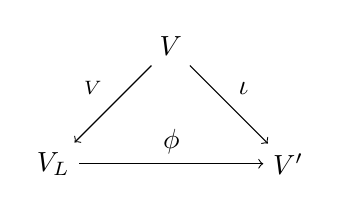
\begin{tikzpicture}[node distance = 6em, auto]
      \node (V) {$V$};
      \node (V_L) [below left of = V] {$V_L$};
      \node (V')  [below right of = V] {$V'$};
      \draw[->] (V) to node[swap] {$\can_V$} (V_L);
      \draw[->] (V) to node {$\iota$} (V');
      \draw[->] (V_L) to node {$\phi$} (V');
    \end{tikzpicture}
  \end{center}
  commutes and this map is an isomorphism of $L$-vector spaces.
\end{thrm}


That the $\beta_W$ are ``natural'' isomorphisms means the following:
Fixing a $k$-vector space $V$ we have two functors
\[
          F_1, F_2
  \colon  \cVect{L}
  \to     \cVect{k}
\]
where $F_1(W) \coloneqq \Hom_L(V_L,W)$ for every $L$-vector space $W$ and for every $L$-linear map $f \colon W \to W'$
\[
          F_1(f)
  \colon  \Hom_L(V_L, W)
  \to     \Hom_L(V_L, W'),
  \quad   h
  \mapsto f \circ h,
\]
as well as $F_2(W) \coloneqq \Hom_k(V,W)$ for every $L$-vector space $W$ and for every $L$-linear map $f \colon W \to W'$
\[
          F_2(f)
  \colon  \Hom_k(V,W)
  \to     \Hom_k(V,W'),
  \quad   h
  \mapsto f \circ h.
\]
The claim is that the $\beta_W$ form an natural isomorphism from $F_1$ to $F_2$, i.e.\ they form a natural transformation from $F_1$ to $F_2$ and $\beta_W$ is an isomorphism for every $L$-vector space $W$.


\begin{proof}
  We will start by proving that $\beta_W$ is an isomorphism of $k$-vector spaces for every $L$-vector space $W$.
  For this we fix an $L$-vector space $W$.
  It is clear that $\Phi \coloneqq \beta_W$ is well-defined and $k$-linear.
  To show that $\Phi$ is an isomorphism we show that
  \[
            \Psi
    \colon  \Hom_k(V,W)
    \to     \Hom_L(V_L, W),
            g
    \mapsto \left(
                      (\lambda \otimes v)
              \mapsto \lambda g(v)
            \right).
  \]
  is an inverse of $\Phi$.
  That $\Psi(g)$ is well-defined and $k$-linear for every map \mbox{$g \in \Hom_k(V,W)$} follows from the fact that the map
  \[
            L \times V
    \to     W,
    \quad   (\lambda, v)
    \mapsto \lambda g(v)
  \]
  is well-defined and $k$-bilinear.
  That $\Psi(g)$ is also $L$-linear is clear.
  That $\Psi$ itself is also $k$-linear is also clear.
  
  Since for all $f \in \Hom_L(V_L,W)$, $\lambda \in L$, $v \in V$
  \begin{align*}
     &\,  (\Psi \Phi)(f)(\lambda \otimes v) \\
    =&\,  \Psi(\Phi(f))(\lambda \otimes v)
    =     \Psi(f \circ \can_V)(\lambda \otimes v) \\
    =&\,  \lambda (f \circ \can_V)(v)
    =     \lambda f(\can_V(v)) \\
    =&\,  \lambda f(1 \otimes v)
    =     f (\lambda \otimes v)
  \end{align*}
  we have $\Psi \Phi = \id_{\Hom_L(V_L, W)}$ and since for all $g \in \Hom_k(V,W$, $v \in V$
  \begin{align*}
        (\Phi \Psi)(g)(v)
    &=  \Phi(\Psi(g))(v)
     =  (\Psi(g) \circ \can_V)(v) \\
    &=  \Psi(g)(\can_V(v))
     =  \Psi(g)(1 \otimes v) \\
    &=  g(v)
  \end{align*}
  we have $\Phi \Psi = \id_{\Hom_k(V,W)}$.
  
  Next we will show that the $\beta_W$ are natural isomorphisms.
  For this we need to check that for all $L$-vector spaces $W$ and $W'$ and every $L$-linear map \mbox{$f \colon W \to W'$} the diagram
  \begin{center}
    \tikzsetnextfilename{naturalisomorphism}
    \begin{tikzpicture}[node distance = 6em, auto]
      \node (HomLW) {$\Hom_L(V_L, W)$};
      \node (HomLW') [right = 6em of HomLW] {$\Hom_L(V_L, W')$};
      \node (HomkW) [below of = HomLW] {$\Hom_k(V,W)$};
      \node (HomkW') [below of = HomLW'] {$\Hom_k(V,W')$};
      \draw[->] (HomLW) to node {$F_1(f)$} (HomLW');
      \draw[->] (HomkW) to node[swap] {$F_2(f)$} (HomkW');
      \draw[->] (HomLW) to node[swap] {$\beta_W$} (HomkW);
      \draw[->] (HomLW') to node {$\beta_{W'}$} (HomkW');
    \end{tikzpicture}
  \end{center}
  commutes, where $F_1$ and $F_2$ are defined as in the previous explanation.
  This is clear, since $F_1(f)$ and $F_2(f)$ are precomposing with $f$ and $\beta_W$ and $\beta_{W'}$ are composing with $\can_V$, and therefore for all $h \in \Hom_L(V_L, W)$
  \begin{align*}
     &\,  (F_2(f) \circ \beta_W)(h)
    =     F_2(f)(\beta_W(h)) \\
    =&\,  F_2(f)(h \circ \can_V)
    =     f \circ (h \circ \can_V) \\
    =&\,  (f \circ h) \circ \can_V
    =     \beta_{W'}(f \circ h) \\
    =&\,  \beta_{W'}(F_1(f)(h))
    =     (\beta_{W'} \circ F_1(f))(h) \,.
  \end{align*}
  
  All that’s left to show is that property defines $V_L$ uniquely up to unique isomorphism.
  To prove this let $V'$ be an $L$-vector space together with a $k$-linear map $\iota \colon V \to V'$ such that for every $L$-vector space $W$ the map
  \[
            \alpha_W
    \colon  \Hom_L(V', W)
    \to     \Hom_k(V, W),
    \quad   f
    \mapsto f \circ \iota
  \]
  is an isomorphism of $k$-vector spaces.
  
  First we notice that
  \[
            \Hom_L(V_L, V_L)
    \cong   \Hom_k(V, V_L),
    \quad   f
    \mapsto f \circ \can_V.
  \]
  Therefore there exists exactly one $f \in \Hom_L(V_L, V_L)$ with $f \circ \can_V = \can_V$.
  It is clear that $f = \id_{V_L}$.
  In the same way we find that $g \in \Hom_L(V', V')$ with $g \circ \iota = \iota$ if and only if $g = \id_{V'}$.
  
  Next we notice that
  \[
          \Hom_L(V_L, V')
    \cong \Hom_k(V, V'),
            f
    \mapsto f \circ \can_V.
  \]
  Therefore there exists a unique $L$-linear map $\phi \in \Hom_L(V_L, V')$ such that \mbox{$\iota = \phi \circ \can_V$}.
  All that’s left to check is that $\phi$ is an isomorphism.
  For this we find in same way that there exists a unique $L$-linear map $\psi \in \Hom_L(V', V_L)$ with $\can_V = \psi \circ \iota$.
  Since
  \[
      \phi \psi \circ \iota
    = \phi \circ \can_V
    = \iota
  \]
  as well as
  \[
      \psi \phi \circ \can_V
    = \psi \circ \iota
    = \can_V
  \]
  we find by the previous observations that $\phi \psi = \id_{V'}$ and $\psi \phi = \id_{V_L}$.
\end{proof}


Recall the following from linear algebra:


\begin{rec}
  Let $k$ be a field and $V$ a $k$-vector space.
  Then $B \subseteq V$ is a $k$-basis of $V$ if and only if for every $k$-vector space $W$ the restriction
  \[
        \Hom_k(V,W
    \to \Maps(B,W),
    \quad   f
    \mapsto f_{|B}
  \]
  is a bijection.
\end{rec}


\begin{lem}
  Let $V$ be a $k$-vector space.
  Then $\{v_i\}_{i \in I}$ is a $k$-basis of $V$ if and only if $\{1 \otimes v_i\}_{i \in I}$ is an $L$-basis of $V_L$.
\end{lem}
\begin{proof}
  Since $\can_V \colon V \to V_L$ is injective it induces a bijection
  \[
            \phi
    \colon  \{v_i\}_{i \in I}
    \to     \{1 \otimes v_i\}_{i \in I},
            v_i
    \mapsto 1 \otimes v_i
    =       \can_V(v_i)
  \]
  For every $L$-vector space $W$ we therefore get a commutative diagram
  \begin{center}
    \tikzsetnextfilename{scalar_extension_and_bases}
    \begin{tikzpicture}[node distance = 6em, auto]
      \node (HomL) {$\Hom_L(V_L, W)$};
      \node (Homk) [right = 6em of HomL] {$\Hom_k(V,W)$};
      \node (MapsL) [below of = HomL] {$\Maps\left( \{1 \otimes v_i\}_{i \in I}, W\right )$};
      \node (Mapsk) [below of = Homk] {$\Maps\left( \{v_i\}_{i \in I} ,W\right )$};
      \draw[double equal sign distance] (HomL) to node {$\sim$} (Homk);
      \draw[double equal sign distance] (MapsL) to node {$\sim$} (Mapsk);
      \draw[->] (HomL) to node[swap] {restriction} (MapsL);
      \draw[->] (Homk) to node {restriction} (Mapsk);
    \end{tikzpicture}
  \end{center}
  where we have an isomorphism of $k$-vector spaces
  \[
            \Hom_L(V_L, W)
    \cong   \Hom_k(V, W),
    \quad   h
    \mapsto h \circ \can_V \,,
  \]
  and the bijection
  \[
          \Maps\left( \{1 \otimes v_i\}_{i \in I}, W \right)
    \cong \Maps\left( \{v_i\}_{i \in I} ,W \right),
    \quad   h
    \mapsto h \circ \phi \,.
  \]
  That $\{v_i\}_{i \in I}$ is a $k$-basis of $V$ is equivalent to saying that the restriction on the right side is a bijection and that $\{1 \otimes v_i\}_{i \in I}$ is an $L$-basis of $V_L$ is equivalent to saying that the restriction on the left side is a bijection.
  Since the diagram commutes these two are equivalent.
\end{proof}


\begin{cor}\label{cor: inclusion to bijection vector spaces}
  Let $V$ be an $L$-vector space, $U \subseteq V$ a $k$-vector subspace and $B \subseteq U$, such that $B$ is a $k$-basis of $U$ and an $L$-basis of $V$.
  Then
  \[
            \phi
    \colon  U_L
    \colon  V,
    \quad   \lambda \otimes u
    \mapsto \lambda u
  \]
  is an isomorphism of $L$-vector spaces.
\end{cor}
\begin{proof}
  $\phi$ is the $L$-linear map that corresponds to the $k$-linear inclusion $U \hookrightarrow V$.
  Therefore it maps the $L$-basis $\{1 \otimes b\}_{b \in B}$ of $U_L$ bijectively to the $L$-basis $B$ of $V$.
\end{proof}


\begin{lem}
  Let $V$ be a $k$-vector space and $\{U_i\}_{i \in I}$ a collection of $k$-vector subspaces $U_i \subseteq V$.
  Then
  \[
      L \otimes_k \bigcap_{i \in I} U_i
    = \bigcap_{i \in I} L \otimes_k U_i \,.
  \]
\end{lem}
\begin{proof}
  {[A proof will be added later.]}
\end{proof}





\section{Functoriality}


Given $k$-vector spaces $V$ and $W$ and a $k$-linear map $f \colon V \to W$ we get a $k$-linear map
\[
            f_L
  \coloneqq \id_L \otimes f
  \colon    V_L
  \to       W_L.
\]
It is easy to check that $f_L$ is also $L$-linear.
Therefore we can understand the extension of scalars as a functor
\[
  E \colon \cVect{k} \to \cVect{L}
\]
with $E(V) = V_L$ for every $k$-vector space $V$ and $E(f) = f_L$ for every $k$-linear map $f$. 

\begin{lem}
  Let $V$ and $V'$ be $k$-vector spaces.
  For every $k$-linear map $f \colon V \to V'$
  \tikzsetnextfilename{can_and_fL_commute}
  \begin{center}
    \begin{tikzpicture}[node distance = 6em, auto]
      \node (V) {$V$};
      \node (V') [right of = V] {$V'$};
      \node (VL) [below of = V] {$V_L$};
      \node (V'L) [below of = V'] {$V'_L$};
      \draw[->] (V) to node {$f$} (V');
      \draw[->] (VL) to node {$f_L$} (V'L);
      \draw[->] (V) to node[swap] {$\can_V$} (VL);
      \draw[->] (V') to node {$\can_{V'}$} (V'L);
    \end{tikzpicture}
  \end{center}
  commutes.
\end{lem}
\begin{proof}
  This can easily be checked by calculation, since for all $v \in V$
  \begin{align*}
        (f_L \circ \can_V)(v)
    &=  f_L(\can_V(v))
     =  f_L(1 \otimes v) \\
    &=  1 \otimes f(v)
     =  \can_{V'}(f(v))
     =  (\can_{V'} \circ f)(v) \,.
    \qedhere
  \end{align*}
\end{proof}


We also have the restriction of scalars as a functor
\[
  R \colon \cVect{L} \to \cVect{k}
\]
which sends every $L$-vector space to its underlying $k$-vector space and every $L$-linear map to the corresponding $k$-linear map.
  
From the universal property of the extension of scalars we know that for every $k$-vector space $V$ and $L$-vector space $W$ we have an isomorphism
\[
          \Phi_{V,W}
  \colon  \Hom_L(E(V),W)
  \cong   \Hom_k(V,R(W))
\]
of $k$-vector spaces.
This observation results in the following proposition:
  
\begin{prop}
  $E$ is left adjoint to $R$ via the bijections $\Phi_{V,W}$.
\end{prop}
\begin{proof}
  We need to check that for all $k$-vector spaces $V$ and $V'$, all $L$-vector spaces $W$ and $W'$, every $k$-linear map $f \colon V' \to V$ (notice that $f$ goes from $V'$ to $V$) and every $L$-linear map $g \colon W \to W'$ the diagram
  \tikzsetnextfilename{scalar_extension_and_restriction_adjoint}
  \begin{center}
    \begin{tikzpicture}[node distance = 6em, auto]
      \node (L) {$\Hom_L(V_L, W)$};
      \node (L') [right = 6em of L] {$\Hom_L(V'_L, W')$};
      \node (k) [below of = L] {$\Hom_k(V,W)$};
      \node (k') [below of = L'] {$\Hom_k(V', W')$};
      \draw[->] (L) to node {$g \circ - \circ f_L$} (L');
      \draw[->] (k) to node[swap] {$g \circ - \circ f$} (k');
      \draw[->] (L) to node[swap] {$\Phi_{V,W}$} (k);
      \draw[->] (L') to node {$\Phi_{V',W'}$} (k');
    \end{tikzpicture}
  \end{center}
  commutes.
  Since $\Phi_{V,W} = - \circ \can_V$ and $\Phi_{V,W'} = - \circ \can_{V'}$ this follows from $\can_{V'} \circ f_L = f \circ \can_V$.
\end{proof}





\section{Extension of Scalars for Algebras}


Given $k$-algebras $A_1$ and $A_2$ their tensor product $A_1 \otimes_k A_2$ is a $k$-algebra via the multiplication
\[
    (a_1 \otimes b_1) \cdot (a_2 \otimes b_2)
  = (a_1 a_2) \otimes (b_1 b_2).
\]
If $A_1$ and $A_2$ are unitial, then so is $A_1 \otimes_k A_2$.
To see that this multiplication is well-defined notice that the map
\begin{align*}
            A_1 \times A_2 \times A_1 \times A_2
  &\to      A_1 \otimes_k A_2 \,, \\
            (a_1, b_1, a_2, b_2)
  &\mapsto  (a_1 a_2) \otimes (b_1 b_2)
\end{align*}
is well-defined and $k$-multilinear, so we get a $k$-linear map
\begin{align*}
            A_1 \otimes_k A_2 \otimes_k A_1 \otimes_k A_2
  &\to      A_1 \otimes_k A_2 \,, \\
            a_1 \otimes b_1 \otimes a_2 \otimes b_2
  &\mapsto  (a_1 a_2) \otimes (b_1 b_2) \,,
\end{align*}
which under the isomorphism of $k$-vector spaces
\[
        A_1 \otimes_k A_2 \otimes_k A_1 \otimes_k A_2
  \cong (A_1 \otimes_k A_2) \otimes_k (A_1 \otimes_k A_2)
\]
corresponds to a $k$-bilinear map
\begin{align*}
            (A_1 \otimes_k A_2) \times (A_1 \otimes_k A_2)
  &\to      A_1 \otimes_k A_2 \,, \\
            (a_1 \otimes b_1, a_2 \otimes b_2)
  &\mapsto  (a_1 a_2) \otimes (b_1 b_2) \,.
\end{align*}


Given a $k$-algebra $A$ we get that $A_L$ is an $L$-vector space and a $k$-algebra.
It is easy to see that that these structures are compatible and give $A_L$ the structure of an $L$-algebra.
To see this compatibility simply notice that the $k$-bilinear map
\begin{align*}
            (A_1 \otimes_k A_2) \times (A_1 \otimes_k A_2)
  &\to      A_1 \otimes_k A_2 \,, \\
            (a_1 \otimes b_1, a_2 \otimes b_2)
  &\mapsto  (a_1 a_2) \otimes (b_1 b_2) \,.
\end{align*}
is also $L$-bilinear.


\begin{rem}
  Let $A$ be a $k$-algebra.
  \begin{enumerate}[label=\emph{\alph*)},leftmargin=*]
    \item
    If $A$ is unital then so is $A_L$.
    \item
    The canonical inclusion $\can_A \colon A \to A_L$ is a homomorphism of $k$-algebras.
  \end{enumerate}
\end{rem}


\begin{lem}
  For $k$-algebras $A_1$ and $A_2$ and a homomorphism of $k$-algebras
  \[
    f \colon A_1 \to A_2
  \]
  the corresponding $L$-linear map
  \[
            f_L
    \colon  L \otimes_k A_1
    \to     L \otimes_k A_2
  \]
  is a homomorphism of $L$-algebras.
\end{lem}
\begin{proof}
  $f_L$ is multiplicative on the simple tensors since for all simple tensors $\lambda_1 \otimes a_1, \lambda_2 \otimes a_2 \in L \otimes_k A_1$
  \begin{align*}
     &\,  f_L((\lambda_1 \otimes a_1)(\lambda_2 \otimes a_2))   \\
    =&\,  f_L((\lambda_1 \lambda_2) \otimes (a_1 a_2))
    =     (\lambda_1 \lambda_2) \otimes f(a_1 a_2) \\
    =&\,  (\lambda_1 \lambda_2) \otimes (f(a_1)f(a_2))
    =     (\lambda_1 \otimes f(a_1)) (\lambda_2 \otimes f(a_2)) \\
    =&\,  f_L(\lambda_1 \otimes a_1) f_L(\lambda_2 \otimes a_2) \,.
  \end{align*}
  Since these simple tensors generate $L \otimes_k A_1$ it follows that $f_L$ is multiplicative.
\end{proof}
  
  
This shows that we can understand the extension of scalars for $k$-algebras als a functor from $\cAlg{k}$ to $\cAlg{L}$.


\begin{lem}
  Let $A$ be a $k$-algebra, $B$ an $L$-algebra and $f \colon A \to B$ a homomorphism of $k$-algebras.
  Then the corresponding $L$-linear map $\hat{f} \colon A_L \to B$ is a homomorphism of $L$-algebras.
  \begin{proof}
  Notice that for all simple tensors $\lambda_1 \otimes a_1, \lambda_2 \otimes a_2 \in A_L$ we have
    \begin{align*}
          \hat{f}((\lambda_1 \otimes a_1)(\lambda_2 \otimes a_2))
      &=  \hat{f}((\lambda_1 \lambda_2) \otimes (a_1 a_2))
       =  \lambda_1 \lambda_2 f(a_1 a_2)    \\
      &=  \lambda_1 \lambda_2 f(a_1) f(a_2)
       =  \lambda_1 f(a_1) \lambda_2 f(a_2) \\
      &=  \hat{f}(\lambda_1 \otimes a_1) \hat{f}(\lambda_2 \otimes a_2) \,.
    \end{align*}
    Since the simple tensors generate $A_L$ it follows that $\hat{f}$ is multiplicative.
  \end{proof}
\end{lem}


\begin{cor}\label{cor: inclusion to bijection algebras}
  Let $B$ be an $L$-algebra, $A \subseteq B$ a $k$-subalgebra and $X \subseteq A$, such that $X$ is a $k$-basis of $A$ and an $L$-basis of $B$.
  Then
  \[
            \phi
    \colon  A_L
    \to     B \,,
    \quad   \lambda \otimes a
    \mapsto \lambda a
  \]
  is an isomorphism of $L$-algebras.
\end{cor}
\begin{proof}
  We know that $\phi$ is a homomorphism of $L$-algebras and we have already seen that $\phi$ is an isomorphism of $L$-vector spaces.
\end{proof}


\begin{lem}
  Let $A$ be a $k$-algebra and $I \subseteq A$ a left-ideal.
  Then $I_L$ is an left-ideal in the $L$-algebra $A_L$.
\end{lem}
\begin{proof}
  Since $I$ is a $k$-vector subspace of $A$ we know that $I_L$ is an $L$-vector subspace of $A_L$.
  For $x \in A_L$ and $y \in I_L$ we have
  \[
    x = \sum_{i=1}^n \lambda_i \otimes a_i
  \]
  with $\lambda_i \in L$ and $a_i \in A$ and
  \[
    y = \sum_{j=1}^m \lambda'_j \otimes a'_j
  \]
  with $\lambda'_j \in L$ and $a'_j \in I$, and therefore
  \begin{align*}
        xy
    &=  \left( \sum_{i=1}^n \lambda_i \otimes a_i \right)
        \left( \sum_{j=1}^m \lambda'_j \otimes a'_j \right) \\
    &=  \sum_{i=1}^n \sum_{j=1}^m (\lambda_i \lambda'_j) \otimes (a_i a'_j)
    \in I_L
  \end{align*}
  This shows that $I_L$ is a left ideal in $A_L$.
\end{proof}


\begin{lem}
  Let $A$ be a $k$-algebra and $I \subseteq A$ a left-sided $k$-ideal generated by elements $(b_j)_{j \in J}$.
  Then the left-sided $L$-ideal $I_L \subseteq A_L$ is generated by the elements $(1 \otimes b_j)_{j \in J}$.
\end{lem}
\begin{proof}
  Let $I_0$ be the left-sided ideal in $A_L$ generated by the elements $(1 \otimes b_j)_{j \in J}$.
  Since $I_L$ is a left-ideal with $1 \otimes b_j \in I_L$ for all $j \in J$ we have $I_0 \subseteq I_L$.
  To show that $I_L \subseteq I_0$ we look at
  \[
              I'
    \coloneqq \{
                a \in A
              \mid
                1 \otimes a \in I_0
              \}
    =         \can_A^{-1}(I_0) \,.
  \]
  $I'$ is a left-sided ideal in $A$ since $\can_A$ is a homomorphism of $k$-algebras.
  Since $1 \otimes b_j \in I_0$ für alle $j \in J$ we have $b_j \in I'$ für alle $j \in J$.
  Since $I$ is the left ideal generated by $(b_j)_{j \in J}$ we have $I \subseteq I'$.
  Therefore we have $1 \otimes a \in I_0$ für alle $a \in I$.
  Since these simple tensors generate $I_L$ as an $L$-vector space we have $I_L \subseteq I_0$.
\end{proof}


\begin{rem}
  We have similar statements about right-sided and two-sided ideals.
\end{rem}


\begin{warn}
  The ideal $(X^2+1)_{\R[X]} \subseteq \R[X]$ is a prime ideal, but the ideal \mbox{$(X^2+1)_{\Complex[X]} \subseteq \Complex[X]$} is not.
\end{warn}





\section{Polynomial Rings and Matrix Rings}


For the polynomial ring $k[X_1, \dotsc, X_n]$ we have an $L$-algebra
\[
    k[X_1, \dotsc, X_n]_L
  = L \otimes_k k[X_1, \dotsc, X_n] \,.
\]
The interesting thing about this algebra is that is it actually $L[X_1, \dotsc, X_n]$.


\begin{prop}
  We have an isomorphism of $L$-algebras
  \[
            \Phi
    \colon  k[X_1, \dotsc, X_n]_L
    \to     L[X_1, \dotsc, X_n]0\,,
    \quad   \lambda \otimes f
    \mapsto \lambda f \,.
  \]
\end{prop}
\begin{proof}
  The monomial $X^\alpha$ with $\alpha \in \N^n$ are a $k$-basis of $k[X_1, \dotsc, X_n]$ and an $L$-basis of $L[X_1, \dotsc, X_n]$ so it follows from corollary \ref{cor: inclusion to bijection algebras}.
\end{proof}


Another interesting example of the extension of scalars is $L \otimes_k \Mat_n(k)$.


\begin{prop}
  We have an isomorphism of $L$-algebras
  \[
    \Phi \colon L \otimes_k \Mat_n(k) \to \Mat_n(L) \,.
  \]
\end{prop}
\begin{proof}
  The matrices $(E_{ij})_{1 \leq i,j \leq n}$ are a $k$-basis of $k[X_1, \dotsc, X_n]$ and an $L$-basis of $L[X_1, \dotsc, X_n]$ so it follows from corollary \ref{cor: inclusion to bijection algebras}.
\end{proof}





\section{Some Backgrounds on Modules and Rings}




\subsection{Noetherian Modules and Rings}


\begin{lemma}
  For an $R$-module $M$ the following conditions are equivalent:
  \begin{enumerate}
    \item
      Every submodule $N \subseteq M$ is finitely generated.
    \item
      Every ascending chain
      \[
                  N_1
        \subseteq N_2
        \subseteq N_3
        \subseteq N_4
        \subseteq \dotsb
      \]
      of submodules $N_i \subseteq M$ stabilizes.
    \item
      Every non-empty family $\mc{S}$ of submodules of $M$ has a maximal ideal, i.e.\ there exists some $N_0 \in \mc{S}$ such that there exists no $N \in \mc{S}$ with $N \supsetneq N_0$.
  \end{enumerate}
\end{lemma}


\begin{definition}
  A ring $R$ is noetherian if it is noetherian as an $R$-module.
\end{definition}


\begin{example}
  LEFT NOTHERIAN BUT NOT RIGHT NOETHERIAN.
\end{example}



\begin{theorem}[Hilbert’s Basis Theorem]
  If $R$ is a noetherian ring, then the polynomial ring $R[X]$ is also noetherian.
\end{theorem}


\begin{example}
  If $k$ is a field then $k[X_1, \dotsc, X_n]$ is noetherian for every $n \geq 0$.
\end{example}


\begin{example}
  COUNTABLE POLYNOMIALRING NOT NOETHERIAN
\end{example}






\subsection{Zariski’s Lemma}
\label{subsection: Zariskis lemma}


\begin{lemma}
  Let $A \subseteq B \subseteq C$ be rings.
  Suppose that $A$ is noetherian, $C$ is finitely generated as an $A$-algebra, and thas $C$ is finitely generated as a $B$-module.
  Then $B$ is also finitely generated as an $A$-algebra.
\end{lemma}


% TODO: Figure out a proof.


\begin{lemma}[Zariski’s Lemma]
  \label{lemma: finitely generated field extensions are algebraic}
  Let $L/k$ be a field extension.
  If $L$ is finitely generated as a $k$-algebra, then the field extension $L/k$ is algebraic and thus finite.
\end{lemma}


% TODO: Figure out a proof.


\begin{example}
  The field extension $k(X)/k$ is not algebraic as $X \in k(X)$ is not algebraic.
  It follows that $k(X)$ is not finitely generated as a $k$-algebra.
\end{example}


\begin{remark}
  That $k(X)$ is not finitely generated as a $k$-algebra can also be seen by hand as follows:
  
  Note that every $f \in k(X)$ with $f \neq 0$ can be uniquely expressed as $f = g/h$ where $g, h \in k[X]$ are coprime polynomial and $h \neq 0$ is monic.
  Also note that whenever we have that $f = g'/h'$ for some polynomials $g', h' \in k[X]$ (which need not be coprime) with $h'$ being monic, then we may write $h' = h'' r$ and $g = g'' r$ where $r \in k[X]$ is the greatest common divisor of $g', h'$.
  Then $f = g'/h' = g''/h''$ with $g', h'$ being coprime and $h'$ being monic, so it follows that $g = g''$ and $h = h''$.
  It follows that every irreducible factor of $h = h''$ must occur in $h'$.
  
  Let $f_1, \dotsc, f_n \in k(X)$ with $f = g_i/h_i$ for polynomials $g_i, h_i \in k[X]$ with $h_i \neq 0$ monic.
  We have that
  \begin{align*}
              k[f_1, \dotsc, f_n]
    &=        k\left[ \frac{g_1}{h_1}, \dotsc, \frac{g_n}{h_n} \right]
     =        k\left[
                \frac{g_1 h_2 \dotsm h_n}{h_1 \dotsm h_n},
                \dotsc,
                \frac{h_1 \dotsm h_{n-1} g_n}{h_1 \dotsm h_n}
              \right] \\
    &\subseteq  \frac{1}{h_1 \dotsm h_n} k[g_1 h_2 \dotsm h_n, h_1 \dotsm h_{n-1} g_n]
     \subseteq  \frac{1}{h_1 \dotsm h_n} k[X] \,,
  \end{align*}
  so every $f \in k[f_1, \dotsc, f_n]$ is of the form $f = g/(h_1 \dotsm h_n)$ for some polynomial $g \in k[X]$.
  It follows that when we write $f = g/h$ for coprime polynomials $g, h \in k[X]$ with $h \neq 0$ monic, then every irreducible factor of $h$ occurs in $h_1 \dotsm h_n$, and is therefore an irreducible factor of some $h_i$.
  
  The polynomial ring $k[X]$ contains infinitely many monic irreducible polynomials, so there exists some irreducible monic polynomial $h \in k[X]$ which does not occur as an irreducible factor of any $h_i$.
  Then $1/h \notin k[f_1, \dotsc, f_n]$ by the above argumentation.
  
  This shows that finitely many elements $f_1, \dotsc, f_n \in k(X)$ cannot generate $k(X)$ as an $k$-algebra.
\end{remark}


\begin{remark}
  The above argumentation shows more generally that $k(X)$ is not finielty generated as an $k[X]$-algebra.
  If $R$ is a unique factorization domain with field of fractions $k$, then the above argumentation can be used to show more even generally that $k$ is finitely generated as an $R$-algebra if and only if $R$ has only finitely many non-associated prime elements.
\end{remark}





\chead{Bibliography} % override previous behavior
\hfuzz=30pt % no overfull hbox warnings in the bibliography
\printbibliography


\end{document}
